% Options for packages loaded elsewhere
\PassOptionsToPackage{unicode}{hyperref}
\PassOptionsToPackage{hyphens}{url}
\PassOptionsToPackage{dvipsnames,svgnames,x11names}{xcolor}
%
\documentclass[
  letterpaper,
  DIV=11,
  numbers=noendperiod]{scrreprt}

\usepackage{amsmath,amssymb}
\usepackage{iftex}
\ifPDFTeX
  \usepackage[T1]{fontenc}
  \usepackage[utf8]{inputenc}
  \usepackage{textcomp} % provide euro and other symbols
\else % if luatex or xetex
  \usepackage{unicode-math}
  \defaultfontfeatures{Scale=MatchLowercase}
  \defaultfontfeatures[\rmfamily]{Ligatures=TeX,Scale=1}
\fi
\usepackage{lmodern}
\ifPDFTeX\else  
    % xetex/luatex font selection
\fi
% Use upquote if available, for straight quotes in verbatim environments
\IfFileExists{upquote.sty}{\usepackage{upquote}}{}
\IfFileExists{microtype.sty}{% use microtype if available
  \usepackage[]{microtype}
  \UseMicrotypeSet[protrusion]{basicmath} % disable protrusion for tt fonts
}{}
\makeatletter
\@ifundefined{KOMAClassName}{% if non-KOMA class
  \IfFileExists{parskip.sty}{%
    \usepackage{parskip}
  }{% else
    \setlength{\parindent}{0pt}
    \setlength{\parskip}{6pt plus 2pt minus 1pt}}
}{% if KOMA class
  \KOMAoptions{parskip=half}}
\makeatother
\usepackage{xcolor}
\setlength{\emergencystretch}{3em} % prevent overfull lines
\setcounter{secnumdepth}{2}
% Make \paragraph and \subparagraph free-standing
\makeatletter
\ifx\paragraph\undefined\else
  \let\oldparagraph\paragraph
  \renewcommand{\paragraph}{
    \@ifstar
      \xxxParagraphStar
      \xxxParagraphNoStar
  }
  \newcommand{\xxxParagraphStar}[1]{\oldparagraph*{#1}\mbox{}}
  \newcommand{\xxxParagraphNoStar}[1]{\oldparagraph{#1}\mbox{}}
\fi
\ifx\subparagraph\undefined\else
  \let\oldsubparagraph\subparagraph
  \renewcommand{\subparagraph}{
    \@ifstar
      \xxxSubParagraphStar
      \xxxSubParagraphNoStar
  }
  \newcommand{\xxxSubParagraphStar}[1]{\oldsubparagraph*{#1}\mbox{}}
  \newcommand{\xxxSubParagraphNoStar}[1]{\oldsubparagraph{#1}\mbox{}}
\fi
\makeatother

\usepackage{color}
\usepackage{fancyvrb}
\newcommand{\VerbBar}{|}
\newcommand{\VERB}{\Verb[commandchars=\\\{\}]}
\DefineVerbatimEnvironment{Highlighting}{Verbatim}{commandchars=\\\{\}}
% Add ',fontsize=\small' for more characters per line
\usepackage{framed}
\definecolor{shadecolor}{RGB}{241,243,245}
\newenvironment{Shaded}{\begin{snugshade}}{\end{snugshade}}
\newcommand{\AlertTok}[1]{\textcolor[rgb]{0.68,0.00,0.00}{#1}}
\newcommand{\AnnotationTok}[1]{\textcolor[rgb]{0.37,0.37,0.37}{#1}}
\newcommand{\AttributeTok}[1]{\textcolor[rgb]{0.40,0.45,0.13}{#1}}
\newcommand{\BaseNTok}[1]{\textcolor[rgb]{0.68,0.00,0.00}{#1}}
\newcommand{\BuiltInTok}[1]{\textcolor[rgb]{0.00,0.23,0.31}{#1}}
\newcommand{\CharTok}[1]{\textcolor[rgb]{0.13,0.47,0.30}{#1}}
\newcommand{\CommentTok}[1]{\textcolor[rgb]{0.37,0.37,0.37}{#1}}
\newcommand{\CommentVarTok}[1]{\textcolor[rgb]{0.37,0.37,0.37}{\textit{#1}}}
\newcommand{\ConstantTok}[1]{\textcolor[rgb]{0.56,0.35,0.01}{#1}}
\newcommand{\ControlFlowTok}[1]{\textcolor[rgb]{0.00,0.23,0.31}{\textbf{#1}}}
\newcommand{\DataTypeTok}[1]{\textcolor[rgb]{0.68,0.00,0.00}{#1}}
\newcommand{\DecValTok}[1]{\textcolor[rgb]{0.68,0.00,0.00}{#1}}
\newcommand{\DocumentationTok}[1]{\textcolor[rgb]{0.37,0.37,0.37}{\textit{#1}}}
\newcommand{\ErrorTok}[1]{\textcolor[rgb]{0.68,0.00,0.00}{#1}}
\newcommand{\ExtensionTok}[1]{\textcolor[rgb]{0.00,0.23,0.31}{#1}}
\newcommand{\FloatTok}[1]{\textcolor[rgb]{0.68,0.00,0.00}{#1}}
\newcommand{\FunctionTok}[1]{\textcolor[rgb]{0.28,0.35,0.67}{#1}}
\newcommand{\ImportTok}[1]{\textcolor[rgb]{0.00,0.46,0.62}{#1}}
\newcommand{\InformationTok}[1]{\textcolor[rgb]{0.37,0.37,0.37}{#1}}
\newcommand{\KeywordTok}[1]{\textcolor[rgb]{0.00,0.23,0.31}{\textbf{#1}}}
\newcommand{\NormalTok}[1]{\textcolor[rgb]{0.00,0.23,0.31}{#1}}
\newcommand{\OperatorTok}[1]{\textcolor[rgb]{0.37,0.37,0.37}{#1}}
\newcommand{\OtherTok}[1]{\textcolor[rgb]{0.00,0.23,0.31}{#1}}
\newcommand{\PreprocessorTok}[1]{\textcolor[rgb]{0.68,0.00,0.00}{#1}}
\newcommand{\RegionMarkerTok}[1]{\textcolor[rgb]{0.00,0.23,0.31}{#1}}
\newcommand{\SpecialCharTok}[1]{\textcolor[rgb]{0.37,0.37,0.37}{#1}}
\newcommand{\SpecialStringTok}[1]{\textcolor[rgb]{0.13,0.47,0.30}{#1}}
\newcommand{\StringTok}[1]{\textcolor[rgb]{0.13,0.47,0.30}{#1}}
\newcommand{\VariableTok}[1]{\textcolor[rgb]{0.07,0.07,0.07}{#1}}
\newcommand{\VerbatimStringTok}[1]{\textcolor[rgb]{0.13,0.47,0.30}{#1}}
\newcommand{\WarningTok}[1]{\textcolor[rgb]{0.37,0.37,0.37}{\textit{#1}}}

\providecommand{\tightlist}{%
  \setlength{\itemsep}{0pt}\setlength{\parskip}{0pt}}\usepackage{longtable,booktabs,array}
\usepackage{calc} % for calculating minipage widths
% Correct order of tables after \paragraph or \subparagraph
\usepackage{etoolbox}
\makeatletter
\patchcmd\longtable{\par}{\if@noskipsec\mbox{}\fi\par}{}{}
\makeatother
% Allow footnotes in longtable head/foot
\IfFileExists{footnotehyper.sty}{\usepackage{footnotehyper}}{\usepackage{footnote}}
\makesavenoteenv{longtable}
\usepackage{graphicx}
\makeatletter
\def\maxwidth{\ifdim\Gin@nat@width>\linewidth\linewidth\else\Gin@nat@width\fi}
\def\maxheight{\ifdim\Gin@nat@height>\textheight\textheight\else\Gin@nat@height\fi}
\makeatother
% Scale images if necessary, so that they will not overflow the page
% margins by default, and it is still possible to overwrite the defaults
% using explicit options in \includegraphics[width, height, ...]{}
\setkeys{Gin}{width=\maxwidth,height=\maxheight,keepaspectratio}
% Set default figure placement to htbp
\makeatletter
\def\fps@figure{htbp}
\makeatother
% definitions for citeproc citations
\NewDocumentCommand\citeproctext{}{}
\NewDocumentCommand\citeproc{mm}{%
  \begingroup\def\citeproctext{#2}\cite{#1}\endgroup}
\makeatletter
 % allow citations to break across lines
 \let\@cite@ofmt\@firstofone
 % avoid brackets around text for \cite:
 \def\@biblabel#1{}
 \def\@cite#1#2{{#1\if@tempswa , #2\fi}}
\makeatother
\newlength{\cslhangindent}
\setlength{\cslhangindent}{1.5em}
\newlength{\csllabelwidth}
\setlength{\csllabelwidth}{3em}
\newenvironment{CSLReferences}[2] % #1 hanging-indent, #2 entry-spacing
 {\begin{list}{}{%
  \setlength{\itemindent}{0pt}
  \setlength{\leftmargin}{0pt}
  \setlength{\parsep}{0pt}
  % turn on hanging indent if param 1 is 1
  \ifodd #1
   \setlength{\leftmargin}{\cslhangindent}
   \setlength{\itemindent}{-1\cslhangindent}
  \fi
  % set entry spacing
  \setlength{\itemsep}{#2\baselineskip}}}
 {\end{list}}
\usepackage{calc}
\newcommand{\CSLBlock}[1]{\hfill\break\parbox[t]{\linewidth}{\strut\ignorespaces#1\strut}}
\newcommand{\CSLLeftMargin}[1]{\parbox[t]{\csllabelwidth}{\strut#1\strut}}
\newcommand{\CSLRightInline}[1]{\parbox[t]{\linewidth - \csllabelwidth}{\strut#1\strut}}
\newcommand{\CSLIndent}[1]{\hspace{\cslhangindent}#1}

\KOMAoption{captions}{tableheading,figureheading}
\makeatletter
\@ifpackageloaded{tcolorbox}{}{\usepackage[skins,breakable]{tcolorbox}}
\@ifpackageloaded{fontawesome5}{}{\usepackage{fontawesome5}}
\definecolor{quarto-callout-color}{HTML}{909090}
\definecolor{quarto-callout-note-color}{HTML}{0758E5}
\definecolor{quarto-callout-important-color}{HTML}{CC1914}
\definecolor{quarto-callout-warning-color}{HTML}{EB9113}
\definecolor{quarto-callout-tip-color}{HTML}{00A047}
\definecolor{quarto-callout-caution-color}{HTML}{FC5300}
\definecolor{quarto-callout-color-frame}{HTML}{acacac}
\definecolor{quarto-callout-note-color-frame}{HTML}{4582ec}
\definecolor{quarto-callout-important-color-frame}{HTML}{d9534f}
\definecolor{quarto-callout-warning-color-frame}{HTML}{f0ad4e}
\definecolor{quarto-callout-tip-color-frame}{HTML}{02b875}
\definecolor{quarto-callout-caution-color-frame}{HTML}{fd7e14}
\makeatother
\makeatletter
\@ifpackageloaded{bookmark}{}{\usepackage{bookmark}}
\makeatother
\makeatletter
\@ifpackageloaded{caption}{}{\usepackage{caption}}
\AtBeginDocument{%
\ifdefined\contentsname
  \renewcommand*\contentsname{Table of contents}
\else
  \newcommand\contentsname{Table of contents}
\fi
\ifdefined\listfigurename
  \renewcommand*\listfigurename{List of Figures}
\else
  \newcommand\listfigurename{List of Figures}
\fi
\ifdefined\listtablename
  \renewcommand*\listtablename{List of Tables}
\else
  \newcommand\listtablename{List of Tables}
\fi
\ifdefined\figurename
  \renewcommand*\figurename{Figure}
\else
  \newcommand\figurename{Figure}
\fi
\ifdefined\tablename
  \renewcommand*\tablename{Table}
\else
  \newcommand\tablename{Table}
\fi
}
\@ifpackageloaded{float}{}{\usepackage{float}}
\floatstyle{ruled}
\@ifundefined{c@chapter}{\newfloat{codelisting}{h}{lop}}{\newfloat{codelisting}{h}{lop}[chapter]}
\floatname{codelisting}{Listing}
\newcommand*\listoflistings{\listof{codelisting}{List of Listings}}
\usepackage{amsthm}
\theoremstyle{definition}
\newtheorem{exercise}{Exercise}[chapter]
\theoremstyle{remark}
\AtBeginDocument{\renewcommand*{\proofname}{Proof}}
\newtheorem*{remark}{Remark}
\newtheorem*{solution}{Solution}
\newtheorem{refremark}{Remark}[chapter]
\newtheorem{refsolution}{Solution}[chapter]
\makeatother
\makeatletter
\makeatother
\makeatletter
\@ifpackageloaded{caption}{}{\usepackage{caption}}
\@ifpackageloaded{subcaption}{}{\usepackage{subcaption}}
\makeatother

\ifLuaTeX
  \usepackage{selnolig}  % disable illegal ligatures
\fi
\usepackage{bookmark}

\IfFileExists{xurl.sty}{\usepackage{xurl}}{} % add URL line breaks if available
\urlstyle{same} % disable monospaced font for URLs
\hypersetup{
  pdftitle={Pricing and Hedging Derivative Securities: Theory and Methods},
  pdfauthor={Kerry Back; Steven L. Heston; Hong Liu; Mark Loewenstein},
  colorlinks=true,
  linkcolor={blue},
  filecolor={Maroon},
  citecolor={Blue},
  urlcolor={Blue},
  pdfcreator={LaTeX via pandoc}}


\title{Pricing and Hedging Derivative Securities: Theory and Methods}
\author{Kerry Back \and Steven L. Heston \and Hong Liu \and Mark
Loewenstein}
\date{}

\begin{document}
\maketitle

\renewcommand*\contentsname{Table of contents}
{
\hypersetup{linkcolor=}
\setcounter{tocdepth}{2}
\tableofcontents
}

\bookmarksetup{startatroot}

\chapter*{Preface}\label{preface}
\addcontentsline{toc}{chapter}{Preface}

\markboth{Preface}{Preface}

This is a sequel to \emph{A Course in Derivative Securities:
Introduction to Theory and Computation} published by Springer. It is
currently a work in progress.

\bookmarksetup{startatroot}

\chapter{Calls and Puts}\label{sec-c_calls-puts}

Financial options are rights to buy and sell assets at pre-specified
prices. The rights are traded on exchanges and also as private contracts
(called over-the-counter or OTC). A call option is a right to buy an
asset. A put option is a right to sell an asset. The pre-specified price
is called the exercise price, the strike price, or simply the strike.
The asset to which an option pertains is called the underlying asset,
or, more briefly, the underlying.

Here is a snapshot of market statistics regarding call options on Apple
stock (AAPL) traded on the Chicago Board Options Exchange (CBOE). We are
accessing the data courtesy of Yahoo Finance. We will refer to this data
throughout the chapter.

\begin{Shaded}
\begin{Highlighting}[]
\ImportTok{import}\NormalTok{ pandas }\ImportTok{as}\NormalTok{ pd}
\ImportTok{import}\NormalTok{ yfinance }\ImportTok{as}\NormalTok{ yf}
\ImportTok{from}\NormalTok{ datetime }\ImportTok{import}\NormalTok{ datetime}
\ImportTok{import}\NormalTok{ pytz}
\ImportTok{from}\NormalTok{ datetime }\ImportTok{import}\NormalTok{ datetime}

\NormalTok{est }\OperatorTok{=}\NormalTok{ pytz.timezone(}\StringTok{\textquotesingle{}US/Eastern\textquotesingle{}}\NormalTok{)}
\NormalTok{fmt }\OperatorTok{=} \StringTok{\textquotesingle{}\%Y{-}\%m{-}}\SpecialCharTok{\%d}\StringTok{ \%H:\%M:\%S \%Z\%z\textquotesingle{}}
\NormalTok{now }\OperatorTok{=}\NormalTok{ datetime.today().astimezone(est).strftime(fmt)}

\NormalTok{ticker }\OperatorTok{=} \StringTok{"AAPL"}         \CommentTok{\# ticker to pull}
\NormalTok{kind }\OperatorTok{=} \StringTok{"call"}           \CommentTok{\# call or put}
\NormalTok{maturity }\OperatorTok{=} \DecValTok{4}            \CommentTok{\# option maturity in order of maturities trading}

\NormalTok{tick }\OperatorTok{=}\NormalTok{ yf.Ticker(ticker.upper())}

\CommentTok{\# Pull last stock price}
\NormalTok{close }\OperatorTok{=}\NormalTok{ tick.history().iloc[}\OperatorTok{{-}}\DecValTok{1}\NormalTok{].Close}

\CommentTok{\# Get maturity date}
\NormalTok{date }\OperatorTok{=}\NormalTok{ tick.options[maturity]}

\CommentTok{\# Pull options data}
\NormalTok{df }\OperatorTok{=}\NormalTok{ (}
\NormalTok{    tick.option\_chain(date).calls}
    \ControlFlowTok{if}\NormalTok{ kind }\OperatorTok{==} \StringTok{"call"}
    \ControlFlowTok{else}\NormalTok{ tick.option\_chain(date).puts}
\NormalTok{)}

\NormalTok{df.lastTradeDate }\OperatorTok{=}\NormalTok{ df.lastTradeDate.}\BuiltInTok{map}\NormalTok{(}
    \KeywordTok{lambda}\NormalTok{ x: x.astimezone(est).strftime(fmt)}
\NormalTok{)}

\CommentTok{\# Formatting}
\NormalTok{cols }\OperatorTok{=}\NormalTok{ [}
    \StringTok{"strike"}\NormalTok{,}
    \StringTok{"bid"}\NormalTok{,}
    \StringTok{"ask"}\NormalTok{,}
    \StringTok{"lastPrice"}\NormalTok{,}
    \StringTok{"change"}\NormalTok{,}
    \StringTok{"percentChange"}\NormalTok{,}
    \StringTok{"lastTradeDate"}\NormalTok{,}
    \StringTok{"volume"}\NormalTok{,}
    \StringTok{"openInterest"}\NormalTok{,}
    \StringTok{"impliedVolatility"}\NormalTok{,}
\NormalTok{]}
\NormalTok{df }\OperatorTok{=}\NormalTok{ df[cols]}
\NormalTok{df[}\StringTok{"impliedVolatility"}\NormalTok{] }\OperatorTok{=}\NormalTok{ df[}\StringTok{"impliedVolatility"}\NormalTok{].}\BuiltInTok{map}\NormalTok{(}\StringTok{"}\SpecialCharTok{\{:.1\%\}}\StringTok{"}\NormalTok{.}\BuiltInTok{format}\NormalTok{)}
\NormalTok{df[}\StringTok{"change"}\NormalTok{] }\OperatorTok{=}\NormalTok{ df[}\StringTok{"change"}\NormalTok{].}\BuiltInTok{round}\NormalTok{(}\DecValTok{2}\NormalTok{)}
\NormalTok{df[}\StringTok{"percentChange"}\NormalTok{] }\OperatorTok{=}\NormalTok{ (df[}\StringTok{"percentChange"}\NormalTok{]}\OperatorTok{/}\DecValTok{100}\NormalTok{).}\BuiltInTok{map}\NormalTok{(}\StringTok{"}\SpecialCharTok{\{:.1\%\}}\StringTok{"}\NormalTok{.}\BuiltInTok{format}\NormalTok{)}
\NormalTok{df.columns }\OperatorTok{=}\NormalTok{ [}
    \StringTok{"Strike"}\NormalTok{,}
    \StringTok{"Bid"}\NormalTok{,}
    \StringTok{"Ask"}\NormalTok{,}
    \StringTok{"Last Price"}\NormalTok{,}
    \StringTok{"Change"}\NormalTok{,}
    \StringTok{"\% Change"}\NormalTok{,}
    \StringTok{"Time of Last Trade"}\NormalTok{,}
    \StringTok{"Volume"}\NormalTok{,}
    \StringTok{"Open Interest"}\NormalTok{,}
    \StringTok{"Implied Volatility"}\NormalTok{,}
\NormalTok{] }
\NormalTok{df }\OperatorTok{=}\NormalTok{ df.set\_index(}\StringTok{"Strike"}\NormalTok{)}
\BuiltInTok{print}\NormalTok{(}\SpecialStringTok{f"Code was executed at }\CharTok{\textbackslash{}t}\SpecialCharTok{\{}\NormalTok{now}\SpecialCharTok{\}}\SpecialStringTok{"}\NormalTok{)}
\BuiltInTok{print}\NormalTok{(}\SpecialStringTok{f"Last }\SpecialCharTok{\{}\NormalTok{ticker}\SpecialCharTok{.}\NormalTok{upper()}\SpecialCharTok{\}}\SpecialStringTok{ price was }\CharTok{\textbackslash{}t}\SpecialStringTok{$}\SpecialCharTok{\{}\NormalTok{close}\SpecialCharTok{:.2f\}}\SpecialStringTok{."}\NormalTok{)}
\BuiltInTok{print}\NormalTok{(}\SpecialStringTok{f\textquotesingle{}Maturity date of options:}\CharTok{\textbackslash{}t}\SpecialCharTok{\{}\NormalTok{date}\SpecialCharTok{\}}\SpecialStringTok{\textquotesingle{}}\NormalTok{)}
\NormalTok{pd.set\_option(}\StringTok{\textquotesingle{}display.max\_rows\textquotesingle{}}\NormalTok{, }\DecValTok{500}\NormalTok{)}
\NormalTok{pd.set\_option(}\StringTok{\textquotesingle{}display.max\_columns\textquotesingle{}}\NormalTok{, }\DecValTok{500}\NormalTok{)}
\NormalTok{pd.set\_option(}\StringTok{\textquotesingle{}display.width\textquotesingle{}}\NormalTok{, }\DecValTok{1000}\NormalTok{)}
\BuiltInTok{print}\NormalTok{(df)}
\end{Highlighting}
\end{Shaded}

\begin{verbatim}
Code was executed at    2024-09-27 09:56:05 EDT-0400
Last AAPL price was     $229.09.
Maturity date of options:   2024-10-25
        Bid  Ask  Last Price  Change % Change            Time of Last Trade  Volume  Open Interest Implied Volatility
Strike                                                                                                               
100.0   0.0  0.0      130.57     0.0     0.0%  2024-09-20 15:55:52 EDT-0400     1.0              1               0.0%
140.0   0.0  0.0       85.28     0.0     0.0%  2024-09-25 14:27:29 EDT-0400     1.0              3               0.0%
145.0   0.0  0.0       89.11     0.0     0.0%  2024-09-20 15:42:03 EDT-0400     5.0              9               0.0%
150.0   0.0  0.0       76.00     0.0     0.0%  2024-09-25 15:28:50 EDT-0400     3.0             74               0.0%
160.0   0.0  0.0       63.21     0.0     0.0%  2024-09-12 12:02:27 EDT-0400     NaN             24               0.0%
165.0   0.0  0.0       55.91     0.0     0.0%  2024-09-09 10:05:45 EDT-0400     NaN              1               0.0%
170.0   0.0  0.0       62.96     0.0     0.0%  2024-09-20 15:52:58 EDT-0400     6.0             10               0.0%
175.0   0.0  0.0       55.17     0.0     0.0%  2024-09-19 13:22:14 EDT-0400     2.0             14               0.0%
180.0   0.0  0.0       48.14     0.0     0.0%  2024-09-26 10:36:07 EDT-0400     1.0             32               0.0%
185.0   0.0  0.0       41.00     0.0     0.0%  2024-09-25 13:47:05 EDT-0400     2.0             15               0.0%
190.0   0.0  0.0       38.78     0.0     0.0%  2024-09-26 15:18:33 EDT-0400     1.0             77               0.0%
195.0   0.0  0.0       33.36     0.0     0.0%  2024-09-26 14:13:45 EDT-0400     2.0             22               0.0%
200.0   0.0  0.0       29.06     0.0     0.0%  2024-09-26 15:59:19 EDT-0400     5.0            425               0.0%
205.0   0.0  0.0       22.60     0.0     0.0%  2024-09-26 09:41:51 EDT-0400     2.0            281               0.0%
210.0   0.0  0.0       19.50     0.0     0.0%  2024-09-26 11:10:34 EDT-0400   180.0            489               0.0%
215.0   0.0  0.0       14.65     0.0     0.0%  2024-09-26 15:54:40 EDT-0400   497.0            963               0.0%
220.0   0.0  0.0       10.60     0.0     0.0%  2024-09-26 15:53:31 EDT-0400   163.0           1574               0.0%
225.0   0.0  0.0        7.15     0.0     0.0%  2024-09-26 15:55:45 EDT-0400   865.0           2275               0.0%
230.0   0.0  0.0        4.60     0.0     0.0%  2024-09-26 15:59:52 EDT-0400  2324.0           4486               0.4%
235.0   0.0  0.0        2.53     0.0     0.0%  2024-09-26 15:59:57 EDT-0400  1792.0           7054               1.6%
240.0   0.0  0.0        1.23     0.0     0.0%  2024-09-26 15:55:10 EDT-0400   885.0          17314               3.1%
245.0   0.0  0.0        0.66     0.0     0.0%  2024-09-26 15:58:44 EDT-0400   320.0           2871               6.3%
250.0   0.0  0.0        0.32     0.0     0.0%  2024-09-26 15:59:59 EDT-0400   223.0           1647               6.3%
255.0   0.0  0.0        0.17     0.0     0.0%  2024-09-26 15:57:48 EDT-0400   110.0            672               6.3%
260.0   0.0  0.0        0.10     0.0     0.0%  2024-09-26 15:59:44 EDT-0400   547.0          15580              12.5%
265.0   0.0  0.0        0.07     0.0     0.0%  2024-09-26 15:28:22 EDT-0400    27.0            169              12.5%
270.0   0.0  0.0        0.03     0.0     0.0%  2024-09-25 15:45:22 EDT-0400    21.0            118              12.5%
275.0   0.0  0.0        0.02     0.0     0.0%  2024-09-26 10:07:51 EDT-0400    50.0             56              12.5%
280.0   0.0  0.0        0.02     0.0     0.0%  2024-09-24 12:13:37 EDT-0400    10.0            155              12.5%
285.0   0.0  0.0        0.01     0.0     0.0%  2024-09-18 13:26:05 EDT-0400     1.0              3              12.5%
290.0   0.0  0.0        0.02     0.0     0.0%  2024-09-25 14:03:52 EDT-0400     1.0             50              12.5%
295.0   0.0  0.0        0.02     0.0     0.0%  2024-09-18 09:30:05 EDT-0400     4.0              9              25.0%
300.0   0.0  0.0        0.02     0.0     0.0%  2024-09-25 14:06:17 EDT-0400    12.0             74              25.0%
\end{verbatim}

\section{Intrinsic Value and Time
Value}\label{intrinsic-value-and-time-value}

\section{Investing in Options}\label{investing-in-options}

\section{Hedging with Options}\label{hedging-with-options}

\section{Selling Options for Income}\label{selling-options-for-income}

\section{Option Spreads}\label{option-spreads}

\section{Put-Call Parity}\label{put-call-parity}

\section{American Options}\label{american-options}

\section{Dividends}\label{dividends}

If the market value of the asset exceeds the exercise price, then we say
the call option is in the money. Buying a call option is a way to bet on
the upside of the underlying asset.

A put option \index{put option} is the right to sell an asset at a
pre-specified (exercise, strike) price. Buying a put is a way to bet on
an asset price becoming low (similar to shorting). A put option is in
the money if the exercise price exceeds the value of the asset. Both
puts and calls are potentially valuable and hence the buyer of a put or
call must pay the seller.

A long put option provides insurance to someone who is long the
underlying asset, because it guarantees that the asset can always be
sold at the strike price of the put (of course, it can be sold at the
market price, if that is higher than the strike of the put).
Symmetrically, a long call option provides insurance to someone who is
short the underlying asset. The terminology in option markets reflects
the parallels between options and insurance contracts. In particular,
the seller of an option is said to write the option and the compensation
(price) he receives from the buyer is called the option premium,
\index{option premium} just as an insurance company writes insurance
contracts in exchange for premium income. Calculating the price at which
one should be willing to trade an option is the main topic of this book.

It is important to recognize the different situations of someone who is
short a call option and someone who is long a put. Both positions are
bets on the downside of the asset. Both the investor who is short a call
and the investor who is long a put may eventually sell the underlying
asset and receive the exercise price in exchange. However, the investor
who is long a put has an option to sell the asset at the exercise price
and the investor who is short a call has an \emph{obligation} to sell
the asset at the exercise price, should the counterparty choose to
exercise the call. Thus, the investor who is long a put will be selling
at the exercise price when it is profitable to do so, whereas the
investor who is short a call will be selling at the exercise price when
it is unprofitable. The buyer of a put must pay the premium to the
seller; he then profits if the asset price is low, with his maximum
possible profit being quite large (the maximum value is attained when
the market value of the underlying asset reaches zero). In contrast, the
seller of a call receives premium income, and the premium is his maximum
possible profit, whereas his potential losses are unbounded. Thus, these
are very different positions.

Individuals who sell calls usually sell out-of-the-money covered calls.
Covered \index{covered call} means that they own the underlying asset
and can therefore deliver the underlying if the call is exercised
without incurring any further expense---they experience only an
opportunity cost in delivering it for less than the market
price.\^{}{[}In contrast, one who sells a call without owning the
underlying is said to sell a naked call.
\index{naked call] The seller of a naked call, or the seller of a put, must post margin, just like a short seller of stocks, in order to ensure that he can meet his obligation.  However, this does not apply to sellers of covered calls.}
A call being out of the money implies that the price of the underlying
must rise before the call would be exercised against the seller; thus,
the seller of an out-of-the money covered call still has some potential
for profit from the underlying. In addition, of course, the seller
receives the premium income from the call. Institutions often follow
this strategy also, using the premium income to enhance their return
from the underlying. One can hedge a short call without owning a full
share of the underlying asset, if one is able to rebalance the hedge
over time. Calculating such hedges is another of the principal topics of
this book.

In a certain sense, option markets are zero-sum games. The profit earned
by one counterparty to an option transaction is a loss suffered by the
other. However, options can allow for an increase in the welfare of all
investors by improving the allocation of risk. A producer who must
purchase a certain input may buy a call option, giving him the right to
buy the input at a fixed price. This caps his expense. The seller of the
call now bears the risk that the input price will be high---in this
case, the option will be exercised and he will be forced to sell at a
price below the market price. It may be that the seller is in a better
position to bear the risk (for example, he may have less of the risk in
his portfolio) and the option transaction may thereby improve the
allocation of risks across investors. The similarity to insurance should
be apparent.

Quite complex bets or hedges can be created by combining options. For
example, a long call and put with the same strike price is called a
straddle. \index{straddle} Such a portfolio is (almost) always in the
money. It is in fact a bet on volatility---a big move in the underlying
asset value away from the exercise price will lead to either the call or
put having a high value. Another important example of an option
portfolio is a collar. \index{collar} A collar consists of a long put
and a short call, or a short call and a long put, with the options
having the same maturity. As mentioned before, a long put provides
insurance to someone who is long the underlying asset. Selling a call
provides premium income that can be used to offset the cost of the put
(the most popular type of collar is a zero-cost collar:
\index{zero-cost collar} a collar in which the premium of the call is
equal to the premium of the put). The cost of selling a call for an
owner of the underlying is that it sells off the upside of the
underlying asset---if the value of the asset exceeds the strike price of
the call, then the call will be exercised and the underlying asset must
be delivered for the strike price (rather than the higher market price).
Thus, one can purchase the downside insurance provided by a long put by
selling part of the upside potential of the asset, rather than paying
the cost of the insurance out of pocket. There are many other examples
of option portfolios that could be given.

Some puts and calls are traded on exchanges. In this case, the exchange
clearinghouse steps between the buyer and seller and becomes the
counterparty to both the buyer and seller. This eliminates the risk that
the seller might default on his obligation when the buyer chooses to
exercise his option. If the owner of an option chooses to exercise, the
clearinghouse randomly chooses someone who is short the option to
fulfill the obligation. Most exchange traded options are never
exercised, because any gain on a long contract can be captured by
selling the contract at the market price, thus cancelling the position.
Obviously, however, the right to exercise is essential, because it
determines the market price. Puts and calls are also transacted over the
counter, \index{over the counter} which means that they are private
contracts of the counterparties. Moreover, puts and calls are embedded
in many other financial instruments. A prosaic but important example is
that most homeowners have the right to pay off their mortgages early.
This means they have call options on their mortgages, with exercise
price equal to the remaining mortgage principal. Similarly, callable
bonds can be redeemed early by the company issuing them, convertible
bonds have embedded call options on the company's stock (which are
exercised by converting the bonds) and there are many, many other
examples. Puts and calls also exist outside financial markets. For
example, a company may begin manufacturing a new product at a small
scale; if the product is successful, the scale can be expanded. In this
case, the company buys a call option on large-scale production with the
premium being the cost of launching small-scale production. Adapting the
methods developed for financial options to value such real options is an
important and growing field. \index{real option}

\subsection{Exercise Policies for Calls and
Puts}\label{exercise-policies-for-calls-and-puts}

It may be rational to exercise a call if the asset value exceeds the
exercise price. Thus, denoting the price of the asset by \(S\) and the
exercise price by \(K\), the owner of a call option can profit by
\(S-K\) dollars by exercising the option when \(S>K\). If \(S<K\),
exercise would be irrational. Thus, the payoff to the owner of the call
option is\footnote{We use the standard notation: \(\max(a,b)\) denotes
  the larger of \(a\) and \(b\) and \(\min(a,b)\) denotes the smaller.}
\(\max(0,S-K)\). It has been said that timing is everything, and the
timing here should be made clearer. The simplest type of option is
called a European option. \index{European option} A European option has
a finite lifetime and can only be exercised at its maturity date. For a
European call option, the exercise strategy just described is the
optimal one, with \(S\) representing the asset price at the maturity
date of the option. Equally, if not more, important are American
options, \index{American option} which can be exercised at any time
before maturity.

For an American call option, the exercise strategy just described is the
optimal one at the maturity date, but it may also be optimal to exercise
prior to maturity. \index{early exercise} Let \(K\) denote the exercise
price, \(T\) the date the option matures, and \(S_T\) the price of the
underlying asset at date \(t \leq T\). The intrinsic value
\index{intrinsic value} of the call option at date \(t\) is defined to
be \(\max(0,S_T-K)\). One would of course never exercise unless the
intrinsic value is positive---i.e., unless the option is in the money.
Moreover, if the asset does not pay a dividend (or other type of cash
flow) prior to the option maturity then one should not exercise in any
circumstances prior to maturity. This is captured in the saying: calls
are better alive than dead. Exercise being suboptimal is equivalent to
the value of the option exceeding the intrinsic value.

The principle that calls on non-dividend-paying assets are better alive
than dead follows from two facts: (i) it is generally a good thing (in
financial markets as well as in life) to keep one's options open, and
(ii) early exercise implies early payment of the exercise price and
hence foregone interest. The usual protest that is heard when this
statement is made is that one should surely exercise if he expects the
stock price to plummet, because by exercising (and then selling the
stock acquired) one can lock in the current stock price rather than
waiting for it to fall, in which case the option will surely be worth
less. This intuition is a reasonable one, but it ignores the fact that
the investor could short sell the stock if he expects it to plummet---he
doesn't need to exercise the option to lock in the current stock price.
In fact, shorting the stock and retaining the option is always better
than exercising, assuming the underlying asset does not pay a dividend.

Specifically, suppose an investor considers exercising at date \(t\). As
an alternative to exercising early, consider shorting the stock at date
\(t\) and retaining the option. This is always better than exercising at
date \(t\), because the short position can be covered (the stock can be
purchased and returned to the lender to cancel the short position) at
cost \(K\) at date \(T\) by exercising the option, and paying \(K\) at
date \(T\) is better than paying it at date \(t\), given that interest
rates must be nonnegative. To be more precise, note that exercise at
date \(t\) produces \(S_T-K\) dollars at date \(t\). On the other hand,
retaining the option, shorting the stock at date \(t\), and covering the
short either by exercising the option or buying the stock in the market
(whichever is cheaper) produces \(S_T\) dollars at date \(t\) and
\[\max(0,S_T-K) - S_T = \max(-S_T, -K) = -\min(S_T,K) \geq -K\] dollars
at date \(T\). If \(S_T>K\), one has \(-K\) dollars at date \(T\), in
which case retaining the option has been superior due to the time value
of money. Furthermore, if \(S_T<K\), the strategy of retaining the
option and shorting the stock produces \(-S_T > -K\) dollars at date
\(T\), so retaining the option is superior due both to flexibility
(waiting until \(T\) to decide whether to exercise turns out to be
better than committing at date \(t\)) and because of the time value of
money.\footnote{Recall that we are assuming investors earn interest on
  the proceeds of short sales; otherwise, the \(S_T\) dollars earned
  from exercising the option and selling the stock will be worth more
  than the \(S_T\) dollars earned from shorting the stock. In this case,
  early exercise could be optimal. However, assuming institutional
  investors can earn interest on the proceeds of shorts, such investors
  should prefer owning the option and shorting the stock to exercising.
  This means they should bid up the price of the option to the point
  where it exceeds the value \(S_T-K\) of exercise. If this is the case,
  then an investor who cannot earn interest on the proceeds of shorts
  should simply sell the option in the market rather than exercise it.
  Thus, a sufficient condition for calls to be better alive than dead is
  that there be some investors who can earn interest on the proceeds of
  shorts. This type of reasoning is possible for each situation in this
  book where the assumption of earning interest on margin deposits is
  important, and we will not deal with it in this much detail again.}

Early exercise of a call option can be optimal when the underlying asset
pays a dividend. The above analysis does not apply in this case, because
paying the dividend to the lender of the stock is an additional cost for
the strategy of retaining the option and shorting the stock. If the
dividend is so small that it cannot offset the time value of money on
the exercise price, then early exercise will not be optimal. In other
cases, deriving the optimal exercise strategy is a complicated problem
that we will first begin to study in
Chapter~\ref{sec-c_introcomputation}.

A European put option will be exercised at its maturity \(T\) if the
price \(S_T\) of the underlying asset is below the exercise price \(K\).
In general, the value at maturity can be expressed as \(\max(0,K-S_T)\).
Early exercise of an American put can be optimal, regardless of whether
the underlying pays a dividend. While it is valuable to keep one's
options open (for puts as well as calls) the time value of money works
in the opposite direction for puts. Early exercise of a put option
implies early receipt of the exercise price, and it is better to receive
cash earlier rather than later. In general, whether early exercise is
optimal depends on how deeply the option is in the money---if the
underlying asset price is sufficiently low, then it will be fairly
certain that exercise will be optimal, whether earlier or late; in this
case, one should exercise earlier to earn interest on the exercise
price. How low it should be to justify early exercise depends on the
interest rate (a higher rate makes the time-value-of-money issue more
important, leading to earlier exercise) and the volatility of the
underlying asset price (a lower volatility reduces the value of keeping
one's options open, leading also to earlier exercise). We will begin to
study the valuation of American puts in
Chapter~\ref{sec-c_introcomputation} also.

\subsection{Compounding Interest}\label{compounding-interest}

During most of the first two parts of the book (the only exception being
Chapter~\ref{sec-c_forwardexchange}) we will assume there is a risk-free
asset earning a constant rate of return. \index{risk-free asset} For
simplicity, we will specify the rate of return as a continuously
compounded rate. \index{continuously compounded interest} For example,
if the annual rate with annual compounding is \(r_a\), then the
corresponding continuously compounded rate is \(r\) defined as
\(r = \log (1+r_a)\), where \(\log\) denotes the natural logarithm
function. This means that the gross return over a year (one plus the
rate of return) is \(\mathrm{e}^r = 1+r_a\). More generally, an
investment of \(x\) dollars for a time period of length \(T\) (we
measure time in years, so, e.g., a six-month investment would mean
\(T=0.5\)) will result in the ownership of \(x\mathrm{e}^{rT}\) dollars
at the end of the time period.

Expressing the interest rate as a continuously compounded rate enables
us to avoid having to specify in each instance whether the rate is for
annual compounding, semi-annual compounding, monthly compounding, etc.
For example, the meaning of an annualized rate \(r_s\) for semi-annual
compounding is that an investment of \(x\) dollars will grow over a year
to \(x(1+r_s/2)^2\). The equivalent continuously compounded rate is
defined as \(r = \log (1+r_s/2)^2\), and in terms of this rate we can
say that the investment will grow in six months to
\(x\mathrm{e}^{0.5 r}\) and that it will grow in one year to
\(x\mathrm{e}^r\). We can interpret this rate as being continuously
compounded because compounding \(n\) times per year at an annualized
rate of \(r\) results in \$1 growing in a year to \((1+r/n)^n\) and
\[\lim_{n \rightarrow \infty} \left(1+\frac{r}{n}\right)^n = \mathrm{e}^r\;\;.\]
To develop pricing and hedging formulas for derivative securities, it is
a great convenience to assume that investors can trade continuously in
time. This requires us to assume also that returns are computed
continuously. In the case of a risk-free investment of \(x(t)\) dollars
at any date \(t\) at a continuously compounded rate of \(r\), we will
say that the interest earned in an instant \(\mathrm{d} t\) is
\(x(t)r\,\mathrm{d} t\) dollars. This is only meaningful when we
accumulate the interest over a non-infinitesimal period of time. So
consider investing \(x(0)\) dollars at time 0 and reinvesting interest
in the risk-free asset over a time period of length \(T\). Let \(x(t)\)
denote the account balance at date \(t\), for \(0\leq t \leq T\). The
change in the account balance in each instant is the interest earned, so
we have \(\mathrm{d} x(t) = x(t)r\,\mathrm{d} t\). The real meaning of
this equation is that \(x(t)\) satisfies the differential equation
\[\frac{\mathrm{d} x(t)}{\mathrm{d} t} = x(t)r\; ,\] and it is well
known (and easy to verify) that the solution is
\[x(t) = x(0)\mathrm{e}^{rt}\; ,\] leading to an account balance at the
end of the time period of \(x(T) = x(0)\mathrm{e}^{rT}\). Thus, the
statement that the interest earned in an instant \(\mathrm{d} t\) is
\(x(t)r\,\mathrm{d} t\) is equivalent to the statement that interest is
continuously compounded at the rate \(r\).

In the last part of the book, we will drop the assumption that the
risk-free asset earns a constant rate of return. In this case, we will
still generally assume that there is a risk-free asset for very
short-term investments (i.e., for investments with infinitesimal
durations!). We will let \(r(t)\) denote the risk-free rate for an
instantaneous investment at date \(t\). This means that an investment of
\(x(t)\) dollars at date \(t\) in the risk-free asset earns interest in
an instant \(\mathrm{d} t\) equal to \(x(t)r(t)\,\mathrm{d} t\).
Consider again an investment of \(x(0)\) dollars at date 0 in this
instantaneously risk-free asset with interest reinvested and let
\(x(t)\) denote the account balance at date \(t\). Then \(x(t)\) must
satisfy the differential equation
\[\frac{\mathrm{d} x(t)}{\mathrm{d} t} = x(t)r(t)\;\;.\] The solution of
this differential equation is
\[x(t) = x(0)\exp\left(\int_0^t r(s)\,ds\right)\;\;.\] The expression
\(\int_0^t r(s)\,ds\) can be interpreted as a continuous sum over time
of the rates of interest \(r(s)\) earned at times \(s\) between 0 and
\(t\). If these rates are all the same, say equal to \(r\), then
\(\int_0^t r(s)\,ds = rt\) and our compounding factor
\(\exp\left(\int_0^t r(s)\,ds\right)\) is \(\mathrm{e}^{rt}\) as before.

\bookmarksetup{startatroot}

\chapter{Binomial Model and Changes of Measure}\label{sec-c_basics}

This chapter introduces the change of measure (or change of numeraire or
martingale) method for valuing derivative securities. The method is
introduced in a binomial model and then extended to more general
(continuum of states) models. Computations in the more general model
require the continuous-time mathematics presented in
Chapter~\ref{sec-c_continuoustime}.

It should be noted that the pricing and hedging results in this book are
not tied to any particular currency. However, for specificity (and as a
consequence of the author's habit) the discussion will generally be in
terms of dollars. Multiple currencies are addressed in
Chapter~\ref{sec-c_foreignexchange}.

\section{Fundamental Concepts}\label{sec-s_fundamentalconcepts}

\subsection{Longs, Shorts, and Margin}\label{longs-shorts-and-margin}

In financial markets, the owner of an asset is said to be long the
asset. \index{long} If person A owes something to person B, the debt is
an asset to person B but a liability to person A. One also says that
person A is short the asset. \index{short} For example, if someone
borrows money and invests the money in stocks, then the individual is
short cash and long stocks.

One must invest some of one's own money when borrowing money to buy
stocks. For example, an individual could invest \$600, borrow \$400, and
buy \$1000 of stock. The \$600 is called the margin \index{margin}
posted by the investor, and buying stocks in this way is called buying
on margin. The investor, or the portfolio, is also said to be levered,
because buying \$1000 of stock with only a \$600 investment amplifies
the risk and return per dollar of investment. \index{leverage} On a
percentage basis, we would say the account has 60\% margin, the 60\%
being the ratio of the equity (assets minus liabilities = \$1000 of
stock minus \$400 debt) to the assets (\$1000 of stock). If the value of
the stock drops sufficiently far, then it may become doubtful whether
the investor can repay the \$400. In this case, the investor must either
sell the stock or invest more of his own funds (i.e., he receives a
margin call). \index{margin call} In other words, in actual markets
there are margin requirements, \index{margin requirement} that specify a
minimum percent margin an investor must have initially (when borrowing
money) and a minimum percent margin the investor must maintain.

Rather than borrowing money to buy stocks, an investor can do the
opposite---he can borrow stocks to buy money. In this case, buying money
means selling the borrowed stocks for cash. Such an investor will be
short stocks and long cash. This is called short selling (or, more
briefly, shorting) stocks. \index{short selling} For example, suppose
individual A borrows 100 shares of stock from individual B and then
sells them to individual C. Both B and C are long the 100 shares and A
is short, so the net long position is \(2 \times 100 - 100\), which is
the original 100 shares that B was long. A short seller of stocks must
pay to the lender of the stocks any dividends that are paid on the
stock. In our example, both B and C own the 100 shares so both expect to
receive dividends. The company will pay dividends only to C, and A must
pay the dividends to\textasciitilde B.

Of course, investors always wish to buy low and sell high. The usual
method is to buy stocks and hope they rise. An investor who short sells
also wishes to buy low and sell high, but he reverses the order---he
sells first and then hopes the stocks fall. The risk is that the stocks
will instead rise, which will increase the value of his liability (short
stock position) without increasing the value of his assets (long cash
position), thus putting him under water. To shield the lender of the
stocks from this risk, a short seller must also invest some of his own
funds, and this amount is again called the investor's margin. For
example, an investor might invest \$600, and borrow and sell \$1000 of
stock. In this case, the investor will be long \$1600 cash and short
\$1000 worth of stock. His equity is \$600 and his percent margin is
calculated as \$600/\$1000 = 60\%. Again, there are typically both
initial and maintenance margin requirements. An additional feature of
short selling for small individual investors is that they typically will
not earn interest on the proceeds of the short sale (the \$1000 cash
obtained from selling stocks in the above example).

In this book, we will assume there is a single risk-free rate at which
one can both borrow and lend. Moreover, we will assume that investors
earn this rate on margin deposits, including the proceeds of short sales
(and including any margin that may be required when buying and selling
forward and futures contracts). Thus, investors gain from buying on
margin if the asset return is sure to exceed the risk-free rate, and
they gain from short selling if the return on an asset is sure to be
below the risk-free rate. These assumptions are not reasonable for small
individual investors, but they are fairly reasonable for institutional
investors. We will assume that no asset has a return that is certain to
be above the risk-free rate nor certain to be below the risk-free rate,
because institutional investors could arbitrage \index{arbitrage} such
guaranteed high-return or guaranteed low-return assets.

\subsection{Calls and Puts}\label{calls-and-puts}

Call and put options are the basic derivative securities and the
building blocks of many others. A derivative security is a security the
value of which depends upon another security.
\index{derivative security} A call option \index{call option} is the
right to buy an asset at a pre-specified price. The pre-specified price
is called the exercise price, the strike price, or simply the strike.
\index{exercise price} \index{strike price} We will often call the asset
a stock, but there are options on many other types of assets also, and
everything we say will be applicable to those as well.\footnote{One
  caveat is that by asset we mean something that can be stored; thus,
  for example, electricity is, practically speaking, not an asset.} The
asset to which the call option pertains is called the underlying asset,
\index{underlying asset} or, more briefly, the underlying. If the market
value of the asset exceeds the exercise price, then we say the call
option is in the money. Buying a call option is a way to bet on the
upside of the underlying asset.

A put option \index{put option} is the right to sell an asset at a
pre-specified (exercise, strike) price. Buying a put is a way to bet on
an asset price becoming low (similar to shorting). A put option is in
the money if the exercise price exceeds the value of the asset. Both
puts and calls are potentially valuable and hence the buyer of a put or
call must pay the seller.

A long put option provides insurance to someone who is long the
underlying asset, because it guarantees that the asset can always be
sold at the strike price of the put (of course, it can be sold at the
market price, if that is higher than the strike of the put).
Symmetrically, a long call option provides insurance to someone who is
short the underlying asset. The terminology in option markets reflects
the parallels between options and insurance contracts. In particular,
the seller of an option is said to write the option and the compensation
(price) he receives from the buyer is called the option premium,
\index{option premium} just as an insurance company writes insurance
contracts in exchange for premium income. Calculating the price at which
one should be willing to trade an option is the main topic of this book.

It is important to recognize the different situations of someone who is
short a call option and someone who is long a put. Both positions are
bets on the downside of the asset. Both the investor who is short a call
and the investor who is long a put may eventually sell the underlying
asset and receive the exercise price in exchange. However, the investor
who is long a put has an option to sell the asset at the exercise price
and the investor who is short a call has an \emph{obligation} to sell
the asset at the exercise price, should the counterparty choose to
exercise the call. Thus, the investor who is long a put will be selling
at the exercise price when it is profitable to do so, whereas the
investor who is short a call will be selling at the exercise price when
it is unprofitable. The buyer of a put must pay the premium to the
seller; he then profits if the asset price is low, with his maximum
possible profit being quite large (the maximum value is attained when
the market value of the underlying asset reaches zero). In contrast, the
seller of a call receives premium income, and the premium is his maximum
possible profit, whereas his potential losses are unbounded. Thus, these
are very different positions.

Individuals who sell calls usually sell out-of-the-money covered calls.
Covered \index{covered call} means that they own the underlying asset
and can therefore deliver the underlying if the call is exercised
without incurring any further expense---they experience only an
opportunity cost in delivering it for less than the market
price.\^{}{[}In contrast, one who sells a call without owning the
underlying is said to sell a naked call.
\index{naked call] The seller of a naked call, or the seller of a put, must post margin, just like a short seller of stocks, in order to ensure that he can meet his obligation.  However, this does not apply to sellers of covered calls.}
A call being out of the money implies that the price of the underlying
must rise before the call would be exercised against the seller; thus,
the seller of an out-of-the money covered call still has some potential
for profit from the underlying. In addition, of course, the seller
receives the premium income from the call. Institutions often follow
this strategy also, using the premium income to enhance their return
from the underlying. One can hedge a short call without owning a full
share of the underlying asset, if one is able to rebalance the hedge
over time. Calculating such hedges is another of the principal topics of
this book.

In a certain sense, option markets are zero-sum games. The profit earned
by one counterparty to an option transaction is a loss suffered by the
other. However, options can allow for an increase in the welfare of all
investors by improving the allocation of risk. A producer who must
purchase a certain input may buy a call option, giving him the right to
buy the input at a fixed price. This caps his expense. The seller of the
call now bears the risk that the input price will be high---in this
case, the option will be exercised and he will be forced to sell at a
price below the market price. It may be that the seller is in a better
position to bear the risk (for example, he may have less of the risk in
his portfolio) and the option transaction may thereby improve the
allocation of risks across investors. The similarity to insurance should
be apparent.

Quite complex bets or hedges can be created by combining options. For
example, a long call and put with the same strike price is called a
straddle. \index{straddle} Such a portfolio is (almost) always in the
money. It is in fact a bet on volatility---a big move in the underlying
asset value away from the exercise price will lead to either the call or
put having a high value. Another important example of an option
portfolio is a collar. \index{collar} A collar consists of a long put
and a short call, or a short call and a long put, with the options
having the same maturity. As mentioned before, a long put provides
insurance to someone who is long the underlying asset. Selling a call
provides premium income that can be used to offset the cost of the put
(the most popular type of collar is a zero-cost collar:
\index{zero-cost collar} a collar in which the premium of the call is
equal to the premium of the put). The cost of selling a call for an
owner of the underlying is that it sells off the upside of the
underlying asset---if the value of the asset exceeds the strike price of
the call, then the call will be exercised and the underlying asset must
be delivered for the strike price (rather than the higher market price).
Thus, one can purchase the downside insurance provided by a long put by
selling part of the upside potential of the asset, rather than paying
the cost of the insurance out of pocket. There are many other examples
of option portfolios that could be given.

Some puts and calls are traded on exchanges. In this case, the exchange
clearinghouse steps between the buyer and seller and becomes the
counterparty to both the buyer and seller. This eliminates the risk that
the seller might default on his obligation when the buyer chooses to
exercise his option. If the owner of an option chooses to exercise, the
clearinghouse randomly chooses someone who is short the option to
fulfill the obligation. Most exchange traded options are never
exercised, because any gain on a long contract can be captured by
selling the contract at the market price, thus cancelling the position.
Obviously, however, the right to exercise is essential, because it
determines the market price. Puts and calls are also transacted over the
counter, \index{over the counter} which means that they are private
contracts of the counterparties. Moreover, puts and calls are embedded
in many other financial instruments. A prosaic but important example is
that most homeowners have the right to pay off their mortgages early.
This means they have call options on their mortgages, with exercise
price equal to the remaining mortgage principal. Similarly, callable
bonds can be redeemed early by the company issuing them, convertible
bonds have embedded call options on the company's stock (which are
exercised by converting the bonds) and there are many, many other
examples. Puts and calls also exist outside financial markets. For
example, a company may begin manufacturing a new product at a small
scale; if the product is successful, the scale can be expanded. In this
case, the company buys a call option on large-scale production with the
premium being the cost of launching small-scale production. Adapting the
methods developed for financial options to value such real options is an
important and growing field. \index{real option}

\subsection{Exercise Policies for Calls and
Puts}\label{exercise-policies-for-calls-and-puts-1}

It may be rational to exercise a call if the asset value exceeds the
exercise price. Thus, denoting the price of the asset by \(S\) and the
exercise price by \(K\), the owner of a call option can profit by
\(S-K\) dollars by exercising the option when \(S>K\). If \(S<K\),
exercise would be irrational. Thus, the payoff to the owner of the call
option is\footnote{We use the standard notation: \(\max(a,b)\) denotes
  the larger of \(a\) and \(b\) and \(\min(a,b)\) denotes the smaller.}
\(\max(0,S-K)\). It has been said that timing is everything, and the
timing here should be made clearer. The simplest type of option is
called a European option. \index{European option} A European option has
a finite lifetime and can only be exercised at its maturity date. For a
European call option, the exercise strategy just described is the
optimal one, with \(S\) representing the asset price at the maturity
date of the option. Equally, if not more, important are American
options, \index{American option} which can be exercised at any time
before maturity.

For an American call option, the exercise strategy just described is the
optimal one at the maturity date, but it may also be optimal to exercise
prior to maturity. \index{early exercise} Let \(K\) denote the exercise
price, \(T\) the date the option matures, and \(S(t)\) the price of the
underlying asset at date \(t \leq T\). The intrinsic value
\index{intrinsic value} of the call option at date \(t\) is defined to
be \(\max(0,S(t)-K)\). One would of course never exercise unless the
intrinsic value is positive---i.e., unless the option is in the money.
Moreover, if the asset does not pay a dividend (or other type of cash
flow) prior to the option maturity then one should not exercise in any
circumstances prior to maturity. This is captured in the saying: calls
are better alive than dead. Exercise being suboptimal is equivalent to
the value of the option exceeding the intrinsic value.

The principle that calls on non-dividend-paying assets are better alive
than dead follows from two facts: (i) it is generally a good thing (in
financial markets as well as in life) to keep one's options open, and
(ii) early exercise implies early payment of the exercise price and
hence foregone interest. The usual protest that is heard when this
statement is made is that one should surely exercise if he expects the
stock price to plummet, because by exercising (and then selling the
stock acquired) one can lock in the current stock price rather than
waiting for it to fall, in which case the option will surely be worth
less. This intuition is a reasonable one, but it ignores the fact that
the investor could short sell the stock if he expects it to plummet---he
doesn't need to exercise the option to lock in the current stock price.
In fact, shorting the stock and retaining the option is always better
than exercising, assuming the underlying asset does not pay a dividend.

Specifically, suppose an investor considers exercising at date \(t\). As
an alternative to exercising early, consider shorting the stock at date
\(t\) and retaining the option. This is always better than exercising at
date \(t\), because the short position can be covered (the stock can be
purchased and returned to the lender to cancel the short position) at
cost \(K\) at date \(T\) by exercising the option, and paying \(K\) at
date \(T\) is better than paying it at date \(t\), given that interest
rates must be nonnegative. To be more precise, note that exercise at
date \(t\) produces \(S(t)-K\) dollars at date \(t\). On the other hand,
retaining the option, shorting the stock at date \(t\), and covering the
short either by exercising the option or buying the stock in the market
(whichever is cheaper) produces \(S(t)\) dollars at date \(t\) and
\[\max(0,S(T)-K) - S(T) = \max(-S(T), -K) = -\min(S(T),K) \geq -K\]
dollars at date \(T\). If \(S(T)>K\), one has \(-K\) dollars at date
\(T\), in which case retaining the option has been superior due to the
time value of money. Furthermore, if \(S(T)<K\), the strategy of
retaining the option and shorting the stock produces \(-S(T) > -K\)
dollars at date \(T\), so retaining the option is superior due both to
flexibility (waiting until \(T\) to decide whether to exercise turns out
to be better than committing at date \(t\)) and because of the time
value of money.\footnote{Recall that we are assuming investors earn
  interest on the proceeds of short sales; otherwise, the \(S(t)\)
  dollars earned from exercising the option and selling the stock will
  be worth more than the \(S(t)\) dollars earned from shorting the
  stock. In this case, early exercise could be optimal. However,
  assuming institutional investors can earn interest on the proceeds of
  shorts, such investors should prefer owning the option and shorting
  the stock to exercising. This means they should bid up the price of
  the option to the point where it exceeds the value \(S(t)-K\) of
  exercise. If this is the case, then an investor who cannot earn
  interest on the proceeds of shorts should simply sell the option in
  the market rather than exercise it. Thus, a sufficient condition for
  calls to be better alive than dead is that there be some investors who
  can earn interest on the proceeds of shorts. This type of reasoning is
  possible for each situation in this book where the assumption of
  earning interest on margin deposits is important, and we will not deal
  with it in this much detail again.}

Early exercise of a call option can be optimal when the underlying asset
pays a dividend. The above analysis does not apply in this case, because
paying the dividend to the lender of the stock is an additional cost for
the strategy of retaining the option and shorting the stock. If the
dividend is so small that it cannot offset the time value of money on
the exercise price, then early exercise will not be optimal. In other
cases, deriving the optimal exercise strategy is a complicated problem
that we will first begin to study in
Chapter~\ref{sec-c_introcomputation}.

A European put option will be exercised at its maturity \(T\) if the
price \(S(T)\) of the underlying asset is below the exercise price
\(K\). In general, the value at maturity can be expressed as
\(\max(0,K-S(T))\). Early exercise of an American put can be optimal,
regardless of whether the underlying pays a dividend. While it is
valuable to keep one's options open (for puts as well as calls) the time
value of money works in the opposite direction for puts. Early exercise
of a put option implies early receipt of the exercise price, and it is
better to receive cash earlier rather than later. In general, whether
early exercise is optimal depends on how deeply the option is in the
money---if the underlying asset price is sufficiently low, then it will
be fairly certain that exercise will be optimal, whether earlier or
late; in this case, one should exercise earlier to earn interest on the
exercise price. How low it should be to justify early exercise depends
on the interest rate (a higher rate makes the time-value-of-money issue
more important, leading to earlier exercise) and the volatility of the
underlying asset price (a lower volatility reduces the value of keeping
one's options open, leading also to earlier exercise). We will begin to
study the valuation of American puts in
Chapter~\ref{sec-c_introcomputation} also.

\subsection{Compounding Interest}\label{compounding-interest-1}

During most of the first two parts of the book (the only exception being
Chapter~\ref{sec-c_forwardexchange}) we will assume there is a risk-free
asset earning a constant rate of return. \index{risk-free asset} For
simplicity, we will specify the rate of return as a continuously
compounded rate. \index{continuously compounded interest} For example,
if the annual rate with annual compounding is \(r_a\), then the
corresponding continuously compounded rate is \(r\) defined as
\(r = \log (1+r_a)\), where \(\log\) denotes the natural logarithm
function. This means that the gross return over a year (one plus the
rate of return) is \(\mathrm{e}^r = 1+r_a\). More generally, an
investment of \(x\) dollars for a time period of length \(T\) (we
measure time in years, so, e.g., a six-month investment would mean
\(T=0.5\)) will result in the ownership of \(x\mathrm{e}^{rT}\) dollars
at the end of the time period.

Expressing the interest rate as a continuously compounded rate enables
us to avoid having to specify in each instance whether the rate is for
annual compounding, semi-annual compounding, monthly compounding, etc.
For example, the meaning of an annualized rate \(r_s\) for semi-annual
compounding is that an investment of \(x\) dollars will grow over a year
to \(x(1+r_s/2)^2\). The equivalent continuously compounded rate is
defined as \(r = \log (1+r_s/2)^2\), and in terms of this rate we can
say that the investment will grow in six months to
\(x\mathrm{e}^{0.5 r}\) and that it will grow in one year to
\(x\mathrm{e}^r\). We can interpret this rate as being continuously
compounded because compounding \(n\) times per year at an annualized
rate of \(r\) results in \$1 growing in a year to \((1+r/n)^n\) and
\[\lim_{n \rightarrow \infty} \left(1+\frac{r}{n}\right)^n = \mathrm{e}^r\;\;.\]
To develop pricing and hedging formulas for derivative securities, it is
a great convenience to assume that investors can trade continuously in
time. This requires us to assume also that returns are computed
continuously. In the case of a risk-free investment of \(x(t)\) dollars
at any date \(t\) at a continuously compounded rate of \(r\), we will
say that the interest earned in an instant \(\mathrm{d} t\) is
\(x(t)r\,\mathrm{d} t\) dollars. This is only meaningful when we
accumulate the interest over a non-infinitesimal period of time. So
consider investing \(x(0)\) dollars at time 0 and reinvesting interest
in the risk-free asset over a time period of length \(T\). Let \(x(t)\)
denote the account balance at date \(t\), for \(0\leq t \leq T\). The
change in the account balance in each instant is the interest earned, so
we have \(\mathrm{d} x(t) = x(t)r\,\mathrm{d} t\). The real meaning of
this equation is that \(x(t)\) satisfies the differential equation
\[\frac{\mathrm{d} x(t)}{\mathrm{d} t} = x(t)r\; ,\] and it is well
known (and easy to verify) that the solution is
\[x(t) = x(0)\mathrm{e}^{rt}\; ,\] leading to an account balance at the
end of the time period of \(x(T) = x(0)\mathrm{e}^{rT}\). Thus, the
statement that the interest earned in an instant \(\mathrm{d} t\) is
\(x(t)r\,\mathrm{d} t\) is equivalent to the statement that interest is
continuously compounded at the rate \(r\).

In the last part of the book, we will drop the assumption that the
risk-free asset earns a constant rate of return. In this case, we will
still generally assume that there is a risk-free asset for very
short-term investments (i.e., for investments with infinitesimal
durations!). We will let \(r(t)\) denote the risk-free rate for an
instantaneous investment at date \(t\). This means that an investment of
\(x(t)\) dollars at date \(t\) in the risk-free asset earns interest in
an instant \(\mathrm{d} t\) equal to \(x(t)r(t)\,\mathrm{d} t\).
Consider again an investment of \(x(0)\) dollars at date 0 in this
instantaneously risk-free asset with interest reinvested and let
\(x(t)\) denote the account balance at date \(t\). Then \(x(t)\) must
satisfy the differential equation
\[\frac{\mathrm{d} x(t)}{\mathrm{d} t} = x(t)r(t)\;\;.\] The solution of
this differential equation is
\[x(t) = x(0)\exp\left(\int_0^t r(s)\,ds\right)\;\;.\] The expression
\(\int_0^t r(s)\,ds\) can be interpreted as a continuous sum over time
of the rates of interest \(r(s)\) earned at times \(s\) between 0 and
\(t\). If these rates are all the same, say equal to \(r\), then
\(\int_0^t r(s)\,ds = rt\) and our compounding factor
\(\exp\left(\int_0^t r(s)\,ds\right)\) is \(\mathrm{e}^{rt}\) as before.

\section{State Prices in a One-Period Binomial
Model}\label{sec-s_oneperiodbinomial}

To introduce the concepts that will be discussed in the remainder of the
chapter, we will consider in this and the following section the
following very simple framework. \index{binomial model} There is a stock
with price \(S\) today (which we will call date\textasciitilde0). At the
end of some period of time of length \(T\), the stock price will take
one of two values: either \(S_u\) or \(S_d\), where \(S_u > S_d\). If
the stock price equals \(S_u\) we say we are in the up state of the
world, and if it equals \(S_d\) we say we are in the down state. The
stock does not pay a dividend. There is also a risk-free asset earning a
continuously compounded rate of interest \(r\). Finally we want to
consider a European call option on the stock with maturity \(T\) and
strike \(K\). The value of the call option at the end of the period is
\(C_u=\max(0,S_u-K)\) in the up state and \(C_d=\max(0,S_d-K)\) in the
down state.

We will assume
\begin{equation}\phantomsection\label{eq-binomialnoarbitrage}{
\frac{S_u}{S} > \mathrm{e}^{rT} > \frac{S_d}{S}\;.
}\end{equation}

This condition means that the rate of return on the stock in the up
state is greater than the risk-free rate, and the rate of return on the
stock in the down state is less than the risk-free rate. If it were not
true, there would be an arbitrage opportunity: \index{arbitrage} if the
rate of return on the stock were greater than the risk-free rate in both
states, then one should buy an infinite amount of the stock on margin,
and conversely if the rate of return on the stock were less than the
risk-free rate in both states, then one should short an infinite amount
of stock and put the proceeds in the risk-free asset. So what we are
assuming is that there are no arbitrage opportunities in the market for
the stock and risk-free asset.

The delta of the call option is \(\delta = (C_u-C_d)/(S_u-S_d)\).
\index{delta} Multiplying by \(S_u-S_d\) gives us
\(\delta(S_u-S_d) = C_u-C_d\) and rearranging yields
\(\delta S_u - C_u = \delta S_d-C_d\), which is critical to what
follows. Consider purchasing \(\delta\) shares of the stock at date 0
and borrowing
\[\mathrm{e}^{-rT}(\delta S_u-C_u) = \mathrm{e}^{-rT}(\delta S_d-C_d)\]
dollars at date 0. Then you will owe \[\delta S_u-C_u = \delta S_d-C_d\]
dollars at date \(T\), and hence the value of the portfolio at date
\(T\) in the up state will be
\[\text{Value of delta shares} - \text{Dollars owed} = \delta S_u - (\delta S_u-C_u) = C_u\; ,\]
and the value of the portfolio at date \(T\) in the down state will be
\[\text{Value of delta shares} - \text{Dollars owed} = \delta S_d - (\delta S_d-C_d) = C_d\;\;.\]
Thus, this portfolio of buying delta shares and borrowing money (i.e.,
buying delta shares on margin) replicates the call option.
\index{replicating strategy} \index{delta hedge} Consequently, the value
\(C\) of the option at date 0 must be the date--0 cost of the portfolio;
i.e., \begin{equation}\phantomsection\label{eq-C0}{
C = \text{Cost of delta shares} - \text{Dollars borrowed} = \delta S - \mathrm{e}^{-rT}(\delta S_u-C_u)\;.
}\end{equation}

Because the call option is equivalent to buying the stock on margin, it
can be considered a levered investment in the stock. \index{leverage}

We will now rewrite the option pricing Equation~\ref{eq-C0} in terms of
state prices. \index{state price} By substituting for \(\delta\) in
Equation~\ref{eq-C0}, we can rearrange it as

\begin{equation}\phantomsection\label{eq-binomialC1}{
C = \frac{S-\mathrm{e}^{-rT}S_d}{S_u-S_d} \times C_u + \frac{\mathrm{e}^{-rT}S_u-S}{S_u-S_d}\times C_d\; .
}\end{equation}

A little algebra also shows that
\begin{equation}\phantomsection\label{eq-binomialS1}{
S = \frac{S-\mathrm{e}^{-rT}S_d}{S_u-S_d} \times 
S_u + \frac{\mathrm{e}^{-rT}S_u-S}{S_u-S_d}\times S_d\; ,
}\end{equation}

and \begin{equation}\phantomsection\label{eq-binomialR1}{
1 = \frac{S-\mathrm{e}^{-rT}S_d}{S_u-S_d} \times \mathrm{e}^{rT}+ \frac{\mathrm{e}^{-rT}S_u-S}{S_u-S_d}\times \mathrm{e}^{rT}\;.
}\end{equation}

It is convenient to denote the factors appearing in these equations as
\begin{equation}\phantomsection\label{eq-binomialstateprices}{
\pi_u = \frac{S-\mathrm{e}^{-rT}S_d}{S_u-S_d} \quad \text{and} \quad \pi_d = \frac{\mathrm{e}^{-rT}S_u-S}{S_u-S_d}\;.
}\end{equation}

The numbers \(\pi_u\) and \(\pi_d\) are called the state prices, for
reasons that will be explained below.

With these definitions, we can write
Equation~\ref{eq-binomialC1}--Equation~\ref{eq-binomialR1} as

\begin{equation}\phantomsection\label{eq-binomialC2}{
C = \pi_uC_u + \pi_dC_d\;,
}\end{equation}

\begin{equation}\phantomsection\label{eq-binomialS2}{
S = \pi_uS_u+\pi_dS_d\;,
}\end{equation}

\begin{equation}\phantomsection\label{eq-binomialR2}{
1 = \pi_u\mathrm{e}^{rT} + \pi_d \mathrm{e}^{rT}\;.
}\end{equation}

These equations have the following interpretation: the value of a
security today is its value in the up state times \(\pi_u\) plus its
value in the down state times \(\pi_d\). This applies to
Equation~\ref{eq-binomialR2} by considering an investment of \$1 today
in the risk-free asset---it has value 1 today and will have value
\(\mathrm{e}^{rT}\) in both the up and down states at date \(T\).
Moreover, this same equation will hold for any other derivative asset.
For example, if we considered a put option, then a delta--hedging
argument analogous to that we just gave for the call option will lead to
a formula for the value \(P\) of the put today which can be expressed as
\(P = \pi_uP_u+\pi_dP_d\) for the same \(\pi_u\) and \(\pi_d\) defined
in Equation~\ref{eq-binomialstateprices}.

In this model, we can think of any security as a portfolio of what are
called Arrow securities (in recognition of the seminal work of Kenneth
Arrow (Arrow 1964)). \index{Arrow security} One of the Arrow securities
pays \$1 at date \(T\) if the up state occurs and the other pays \$1 at
date \(T\) if the down state occurs. For example, the stock is
equivalent to a portfolio consisting of \(S_u\) units of the first Arrow
security and \(S_d\) units of the second, because the stock is worth
\(S_u\) dollars in the up state and \(S_d\) dollars in the down state.
Equations Equation~\ref{eq-binomialC2}--Equation~\ref{eq-binomialR2}
show that\textasciitilde{} \(\pi_u\) is the price of the first Arrow
security and \(\pi_d\) is the price of the second. For example, the
right-hand side of Equation~\ref{eq-binomialS2} is the value of the
stock at date 0 viewed as a portfolio of Arrow securities when the Arrow
securities have prices \(\pi_u\) and \(\pi_d\). Because the stock
clearly is such a portfolio, its price today must equal its value as
that portfolio, which is what Equation~\ref{eq-binomialS2} asserts.

As mentioned before, the prices \(\pi_u\) and \(\pi_d\) of the Arrow
securities are called the state prices, because they are the prices of
receiving \$1 in the two states of the world. The state prices should be
positive, because the payoff of each Arrow security is nonnegative in
both states and positive in one. A little algebra shows that the
conditions \(\pi_u>0\) and \(\pi_d>0\) are exactly equivalent to our
no-arbitrage assumption Equation~\ref{eq-binomialnoarbitrage}. Thus, we
conclude that \textbf{in the absence of arbitrage opportunities, there
exist positive state prices such that the price of any security is the
sum across the states of the world of its payoff multiplied by the state
price.}

This conclusion generalizes to other models, including models in which
the stock price takes a continuum of possible values. We will discuss
more general models later in this chapter. It is a powerful result that
tremendously simplifies derivative security pricing.

\section{Probabilities and
Numeraires}\label{probabilities-and-numeraires}

In this section, we will continue our analysis of the binomial example.
To apply the statement about state prices appearing in boldface type
above in the most convenient way, we will manipulate the state prices so
we can interpret the sums on the right-hand sides of
Equation~\ref{eq-binomialC2}--Equation~\ref{eq-binomialR2} in terms of
expectations. \index{expectation} The expectation (or mean) of a random
variable is of course its probability-weighted average value.

In general, there are different expectations that are useful. In this
model, there are two that we can define: one corresponding to the
risk-free asset and one corresponding to the stock. Many readers will
have experience with the first in the form of risk-neutral
probabilities.

The risk-neutral probabilities are defined as \(\pi_u\mathrm{e}^{rT}\)
for the up state and \(\pi_d\mathrm{e}^{rT}\) for the down state.
Denoting these as \(p_u\) and \(p_d\) respectively,
Equation~\ref{eq-binomialC2}--Equation~\ref{eq-binomialR2} can be
written as

\begin{equation}\phantomsection\label{eq-binomialC3}{
C = \mathrm{e}^{-rT}[p_uC_u+p_dC_d]\;,
}\end{equation}

\begin{equation}\phantomsection\label{eq-binomialS3}{
S = \mathrm{e}^{-rT}[p_uS_u+p_dS_d]\;,
}\end{equation}

\begin{equation}\phantomsection\label{eq-binomialR3}{
1= p_u+p_d\;.
}\end{equation}

The numbers \(p_u\) and \(p_d\) are both positive (because the state
prices are positive under our no-arbitrage assumption) and
Equation~\ref{eq-binomialR3} states that they sum to one, so it is
indeed sensible to consider them as probabilities. Equations
Equation~\ref{eq-binomialC3} and Equation~\ref{eq-binomialS3} state that
the value of a security today is its expected value at date \(T\) (the
expectation taken with respect to the risk-neutral probabilities)
discounted at the risk-free rate. Thus, these are present value
formulas. Unlike the Capital Asset Pricing Model, for example, there is
no risk premium in the discount rate. This is the calculation we would
do to price assets under the actual probabilities if investors were risk
neutral (or for zero-beta assets). So, we can act as if investors are
risk neutral by adjusting the probabilities. Of course, we are not
really assuming investors are risk neutral. We have simply embedded any
risk premia in the probabilities.\footnote{This fundamental idea is due
  to Cox and Ross (Cox and Ross 1976).}

Equations Equation~\ref{eq-binomialC3} and Equation~\ref{eq-binomialS3}
can be written in an equivalent form, which, though somewhat less
intuitive, generalizes more readily. First, let's introduce some
notation for the price of the risk-free asset. Considering an investment
of \$1 today which grows to \(\mathrm{e}^{rT}\) at date \(T\), it is
sensible to take the price today to be \(R=1\) and the price in the up
and down states at date \(T\) to be
\(R_u=R_d=\mathrm{e}^{rT}\).\footnote{All of the equations appearing
  below will also be true if instead we take \(R=\mathrm{e}^{-rT}\) and
  \(R_u=R_d=1\).} In terms of this notation,
Equation~\ref{eq-binomialC3}--Equation~\ref{eq-binomialR3} can be
written as:

\begin{equation}\phantomsection\label{eq-binomialC4}{
\frac{C}{R} = p_u \frac{C_u}{R_u} + p_d \frac{C_d}{R_d}\;, 
}\end{equation}

\begin{equation}\phantomsection\label{eq-binomialS4}{
\frac{S}{R} = p_u \frac{S_u}{R_u} + p_d \frac{S_d}{R_d}\;, 
}\end{equation}

\begin{equation}\phantomsection\label{eq-binomialR4}{
1=p_u+p_d\;.
}\end{equation}

Each of equations Equation~\ref{eq-binomialC4} and
Equation~\ref{eq-binomialS4} states that the price of a security today
divided by the price of the risk-free asset equals the expected future
value of the same ratio, when we take expectations using the
risk-neutral probabilities. In other words, the mean of the date--\(T\)
value of the ratio is equal to the ratio today. We will discuss the
interpretation and significance of these equations further below. First,
we consider the other type of expectation in this model, which is based
on probabilities corresponding to the stock.

Note that the risk-neutral probabilities are the state prices multiplied
by the gross return on the risk-free asset. Analogously, define numbers
\(q_u = \pi_uS_u/S\) and \(q_d = \pi_dS_d/S\). Substituting for
\(\pi_u\) and \(\pi_d\) in
Equation~\ref{eq-binomialC2}--Equation~\ref{eq-binomialR2} and
continuing to use the notation \(R\) for the price of the risk-free
asset, we obtain

\begin{equation}\phantomsection\label{eq-binomialC5}{
\frac{C}{S} = q_u \frac{C_u}{S_u} + q_d \frac{C_d}{S_d}\;, 
}\end{equation}

\begin{equation}\phantomsection\label{eq-binomialS5}{
1 = q_u + q_d\;,
}\end{equation}

\begin{equation}\phantomsection\label{eq-binomialR5}{
\frac{R}{S} = q_u \frac{R_u}{S_u} + q_d \frac{R_d}{S_d}\;. 
}\end{equation}

Equation Equation~\ref{eq-binomialS5} establishes that we can view the
\(q\)'s as probabilities (like the risk-neutral probabilities, they are
positive because the state prices are positive). Equations
Equation~\ref{eq-binomialC5} and Equation~\ref{eq-binomialR5} both state
that the ratio of a security price to the price of the stock today
equals the mean value of the same ratio at date \(T\), when we compute
expectations using the \(q\)'s as probabilities.

Here is some useful terminology:

\begin{itemize}
\tightlist
\item
  An assignment of probabilities to events is called a
  \emph{probability measure}, or simply a \emph{measure} (because it
  measures the events, in a sense). Thus, we have described two
  different probability measures in this section. \index{measure}
  \index{probability measure}
\item
  The ratio of one price to another is the value of the first
  (numerator) asset when we are using the second (denominator) asset as
  the \emph{numeraire}. \index{numeraire} The term numeraire means a
  unit of measurement. For example, the ratio \(C/S\) is the value of
  the call when we use the stock as the unit of measurement: it is the
  number of shares of stock for which one call option can be exchanged
  (to see this, note that \(C/S\) shares is worth \(C/S \times S = C\)
  dollars, so \(C/S\) shares is worth the same as one call.)
\item
  A variable that changes randomly over time with the expected future
  value being always equal to the current value is called a
  \emph{martingale}. \index{martingale}
\end{itemize}

The right-hand sides of
Equation~\ref{eq-binomialC4}--Equation~\ref{eq-binomialS4} and
Equation~\ref{eq-binomialC5} and Equation~\ref{eq-binomialR5} are
expectations under different \emph{probability measures} (the \(p\)'s or
\(q\)'s). The expected future (date--\(T\)) value equals the current
(date--0) value, so the random variables (\(C/R\) and \(S/R\) or \(C/S\)
and \(R/S\)) are \emph{martingales}. The values \(C/R\) and \(S/R\) are
the values of the call and stock
\emph{using the risk-free asset as numeraire}, and the values \(C/S\)
and \(R/S\) are the values of the call and risk-free asset
\emph{using the stock as numeraire}. Thus, we will express
Equation~\ref{eq-binomialC4}--Equation~\ref{eq-binomialS4} as the call
and stock are martingales when we use the risk-free asset as numeraire.
Likewise, we will express Equation~\ref{eq-binomialC5} and
Equation~\ref{eq-binomialR5} as the call and risk-free asset are
martingales when we use the stock as numeraire. It should be understood
in both cases that using an asset as numeraire means that we also use
the corresponding probability measure (i.e., the \(p\)'s or \(q\)'s). In
general, our conclusion that assets can be priced in terms of positive
state prices when there are no arbitrage opportunities can be rephrased
as: \textbf{if there are no arbitrage opportunities, then for each
(non-dividend-paying) asset, there exists a probability measure such
that the ratio of any other (non-dividend-paying) asset price to the
first (numeraire) asset price is a martingale.}

We have applied this statement to the risk-free asset, which pays
dividends (interest). However, the price \(R_u=R_d=\mathrm{e}^{rT}\)
includes the interest, so no interest has been withdrawn---the interest
has been reinvested---prior to the maturity \(T\) of the option. This is
what we mean by a non-dividend-paying asset. In general, we will apply
the formulas developed in this and the following section to
dividend-paying assets by considering the portfolios in which dividends
are reinvested.

For this exposition, it was convenient to first calculate the state
prices and then calculate the various probabilities. However, that is
not the most efficient way to proceed in most applications. In a typical
application, we would view the prices of the stock and risk-free asset
in the various states of the world as given, and we would be attempting
to compute the value of the call option. Note that the sets of equations
Equation~\ref{eq-binomialC2}--Equation~\ref{eq-binomialR2},
Equation~\ref{eq-binomialC4}--Equation~\ref{eq-binomialR4}, and
Equation~\ref{eq-binomialC5}--Equation~\ref{eq-binomialR5} are all
equivalent. In each case we would consider that there are three
unknowns---the value \(C\) of the call option and either two state
prices or two probabilities. In each case the state prices or
probabilities can be computed from the last two equations in the set of
three equations and then the call value \(C\) can be computed from the
first equation in the set. All three sets of equations produce the same
call value.

In fact, as we will see, it will not even be necessary to calculate the
probabilities. The fact that ratios of non-dividend paying asset prices
to the numeraire asset price are martingales will tell us enough about
the probabilities to calculate derivative values without having to
calculate the probabilities themselves.

We conclude this section with another reformulation of the pricing
relations Equation~\ref{eq-binomialC2}--Equation~\ref{eq-binomialR2}.
This formulation will generalize more easily to pricing when there are a
continuum of states, the subject of the next section.\\
Let \(\text{prob}_u\) denote the actual probability of the up state and
\(\text{prob}_d\) denote the probability of the down state. These
probabilities are irrelevant for pricing derivatives in the binomial
model, but we will use them to write the pricing relations
Equation~\ref{eq-binomialC2}--Equation~\ref{eq-binomialR2} as
expectations with respect to the actual probabilities. To do this, we
can define \begin{align*}
\phi_u &= \frac{\pi_u}{\text{prob}_u}\; ,\\
\phi_d &= \frac{\pi_d}{\text{prob}_d}\;.
\end{align*} Then
Equation~\ref{eq-binomialC2}--Equation~\ref{eq-binomialR2} can be
written as

\begin{equation}\phantomsection\label{eq-binomialC6}{
C = \text{prob}_u\phi_uC_u + \text{prob}_d\phi_dC_d\;,
}\end{equation}

\begin{equation}\phantomsection\label{eq-binomialS6}{
S = \text{prob}_u\phi_uS_u + \text{prob}_d\phi_dS_d\;,
}\end{equation}

\begin{equation}\phantomsection\label{eq-binomialR6}{
R = \text{prob}_u\phi_uR_u + \text{prob}_d\phi_dR_d\;.
}\end{equation}

The right-hand sides are expectations with respect to the actual
probabilities. For example, the right-hand side of
Equation~\ref{eq-binomialC6} is the expectation of the random variable
that equals \(\phi_uC_u\) in the up state and \(\phi_dC_d\) in the down
state. The risk-neutral probabilities can be calculated from \(\phi_u\)
and \(\phi_d\) as \(p_u=\text{prob}_u\phi_uR_u/R\) and
\(p_d=\text{prob}_d\phi_dR_d/R\). Likewise, the probabilities using the
stock as the numeraire can be calculated from \(\phi_u\) and \(\phi_d\)
as \(q_u=\text{prob}_u\phi_uS_u/S\) and
\(q_d=\text{prob}_d\phi_dS_d/S\). In the following section, we will
assume (which can be shown to be true under some technical conditions)
that relations such as
Equation~\ref{eq-binomialC6}--Equation~\ref{eq-binomialR6} hold in a
general (non-binomial) model given the absence of arbitrage
opportunities. We will then show, using definitions analogous to the
definitions of \(p_u\), \(p_d\), \(q_u\), and \(q_d\) in this paragraph,
that relations analogous to
Equation~\ref{eq-binomialC4}--Equation~\ref{eq-binomialR4} and
Equation~\ref{eq-binomialC5}--Equation~\ref{eq-binomialR5} hold.

\section{Asset Pricing with a Continuum of
States}\label{asset-pricing-with-a-continuum-of-states}

In this section, we will define the concepts of state prices and
probabilities corresponding to different numeraires in a more general
framework than that of the preceding section. This leads to what we will
call the fundamental pricing equation, namely Equation~\ref{eq-formula}.
There are really no new concepts in this section, only a bit more
mathematics.

Consider a non-dividend-paying security having the random price \(S(T)\)
at date \(T\). We call the contingencies that affect the price \(S(T)\)
the states of the world. Our principle regarding state prices developed
in the preceding section can in general be expressed as:\footnote{We
  have proven this in the binomial model, but we will not prove it in
  general. As is standard in the literature, we will simply adopt it as
  an assumption. A general proof is in fact difficult and requires a
  definition of no arbitrage that is considerably more complicated than
  the simple assumption Equation~\ref{eq-binomialnoarbitrage} that is
  sufficient in the binomial model.} \textbf{if there are no arbitrage
opportunities, there exists for each date \(T\) a positive random
variable \(\phi(T)\) such that the value at date 0 of a
non-dividend-paying security with price \(S\) is }
\begin{equation}\phantomsection\label{eq-continuum1}{
S(0) = E[\phi(T)S(T)]\;.
}\end{equation}

Here, \(E[\phi(T)S(T)]\) denotes the expectation of the random variable
\(\phi(T)S(T)\). The random variable \(\phi(T)\) is
\index{state price density} called the state price density.\footnote{The
  term density reflects the fact that in each state of the world
  \(\phi(T)\) can be interpreted as the state price per unit of
  probability, just as the normal meaning of density is mass per unit of
  volume.} In a binomial model (or in any model with only a finite
number of states of the world), the concept of an expectation is clear:
it is just a weighted average of outcomes, the weights being the
probabilities. In the binomial model, the right-hand side of
Equation~\ref{eq-binomialS6} is the same as the right-hand side of
Equation~\ref{eq-continuum1}.\footnote{ In general the expectation (or
  mean) of a random variable is an intuitive concept, and an intuitive
  understanding will be sufficient for this book, so I will not give a
  formal definition. It should be understood that we are assuming
  implicitly, whenever necessary, that the expectation exists (which is
  not always the case). In this regard, it is useful to note in passing
  that a product of two random variables \(XY\) has a finite mean
  whenever \(X\) and \(Y\) have finite variances.}

To convert from state prices to probabilities corresponding to different
numeraires, we follow the same procedure as at the end of the previous
section: we multiply together (i) the probability of the state, (ii) the
value of \(\phi(T)\) in the state, and (iii) the gross return of the
numeraire in the state. If there is a continuum of states, then the
actual probability of any individual state will typically be zero, so
this multiplication will produce a zero probability. However, we can
nevertheless add up these probabilities to define the probability of any
event \(A\), an event being a set of states of the world. To do this,
let \(1_A\) denote the random variable that takes the value 1 when \(A\)
is true and which is zero otherwise. Then the probability of \(A\) using
\(S\) as the numeraire is defined as \index{change of measure}
\index{change of numeraire}
\begin{equation}\phantomsection\label{eq-probSnumeraire}{
E\left[1_A\phi(T)\frac{S(T)}{S(0)}\right]\;.
}\end{equation}

This makes sense as a probability because it is nonnegative and because,
if \(A\) is the set of all states of the world, then its probability is
\(E[\phi(T)S(T)/S(0)]\), which equals one by virtue of
Equation~\ref{eq-continuum1}. From Equation~\ref{eq-probSnumeraire} of
the probability of any event \(A\), it can be shown that the expectation
of any random variable \(X\) using \(S\) as the numeraire is
\begin{equation}\phantomsection\label{eq-expSnumeraire}{
E\left[X\phi(T)\frac{S(T)}{S(0)}\right]\;.
}\end{equation}

The use of the symbol \(S\) to denote the price of the numeraire may be
confusing, because \(S\) is usually used to denote a stock price. The
numeraire here could be any non-dividend-paying asset. For example, we
can take \(S(t)=\mathrm{e}^{rt}\), the price of the risk-free asset. The
definition of probabilities as
\begin{equation}\phantomsection\label{eq-riskneutralprob00}{
E[1_A\phi(T)\mathrm{e}^{rT}]
}\end{equation}

will be called the risk-neutral probability measure or simply
risk-neutral measure as before. \index{risk-neutral measure}
\index{risk-neutral probability}

Different numeraires lead to different probability measures and hence to
different expectations. To keep this straight, we will use the numeraire
as a superscript on the expectation symbol: for example, \(E^S\) will
denote expectation with respect to the probability measure that
corresponds to \(S\) being the numeraire. Also, we will use the symbol
\(\text{prob}^S(A)\) to denote the probability of an event \(A\) when we
use \(S\) as the numeraire. So, Equation~\ref{eq-probSnumeraire} and
Equation~\ref{eq-expSnumeraire} will be written as

\begin{equation}\phantomsection\label{eq-probSnumeraire2}{
\text{prob}^S(A) = E\left[1_A\phi(T)\frac{S(T)}{S(0)}\right]\;,
}\end{equation}

\begin{equation}\phantomsection\label{eq-expSnumeraire2}{
E^S[X] = E\left[X\phi(T)\frac{S(T)}{S(0)}\right]\;.
}\end{equation}

Our key result in the preceding section was that the ratio of the price
of any non-dividend paying asset to the price of the numeraire asset is
not expected to change when we use the probability measure corresponding
to the numeraire. We will demonstrate the same result in this more
general model. Recall that \(T\) denotes an arbitrary but fixed date at
which we have defined the probabilities using \(S\) as the numeraire in
Equation~\ref{eq-probSnumeraire}. At each date \(t<T\), let \(E^S_t\)
denote the expectation given information at time \(t\) and using \(S\)
as the numeraire (we will continue to write the expectation at date 0
without a subscript; i.e., \(E^S\) has the same meaning as \(E^S_0\)).
Let \(Y\) denote the price of another non-dividend-paying asset. We will
show that \begin{equation}\phantomsection\label{eq-preformula}{
\frac{Y(t)}{S(t)} = E^S_t \left[\frac{Y(T)}{S(T)}\right]\;.
}\end{equation}

Thus, the expected future (date--\(T\)) value of the ratio \(Y/S\)
always equals the current (date--\(t\)) value when we use \(S\) as the
numeraire. As discussed in the preceding section, the mathematical term
for a random variable whose expected future value always equals its
current value is martingale. Thus, we can express
Equation~\ref{eq-preformula} as stating that the ratio \(Y/S\) is a
martingale when we compute expectations using the probability measure
that corresponds to \(S\) being the numeraire.

The usefulness of Equation~\ref{eq-preformula} is that it gives us a
formula for the asset price \(Y(t)\) at any time \(t\)---and recall that
this formula holds for every non-dividend paying asset. The formula is
obtained from Equation~\ref{eq-preformula} by multiplying through by
\(S(t)\): \begin{equation}\phantomsection\label{eq-formula}{
Y(t) = S(t)E^S_t \left[\frac{Y(T)}{S(T)}\right]\;.
}\end{equation}

\textbf{We will call Equation~\ref{eq-formula}} the fundamental pricing
formula. \index{fundamental pricing formula} It is at the heart of
modern pricing of derivative securities. It is a present value relation:
the value at time \(t\) of the asset is the expectation of its value
\(Y(T)\) at time \(T\) discounted by the (possibly random) factor
\(S(t)/S(T)\). To emphasize that the numeraire can be any
non-dividend-paying asset (and not necessarily a stock price, as the
symbol \(S\) might suggest), we can write Equation~\ref{eq-formula} in
the equivalent form \begin{equation}\phantomsection\label{eq-formula10}{
Y(t) = \text{num}(t)E^\text{num}_t \left[\frac{Y(T)}{\text{num}(T)}\right]\;,
}\end{equation}

where now \(\text{num}(t)\) denotes the price of the
(non-dividend-paying) numeraire asset at time \(t\).

For example, letting \(R(t)\) denote the value \(\mathrm{e}^{rt}\) of
the risk-free asset and using it as the numeraire,
Equation~\ref{eq-formula} becomes
\begin{equation}\phantomsection\label{eq-riskneutralformula}{
Y(t) = \mathrm{e}^{rt}E^R_t\left[\frac{Y(T)}{\mathrm{e}^{rT}}\right] = \mathrm{e}^{-r(T-t)}E^R_t [Y(T)]\;,
}\end{equation}

which means that the value \(Y(t)\) is the expected value of \(Y(T)\)
discounted at the risk-free rate for the remaining time \(T\!-\!t\),
when the expectation is computed under the risk-neutral probability
measure.

We end this section with a proof of Equation~\ref{eq-preformula}, a
proof that the reader may skip if desired.\footnote{The proof is due to
  Harrison and Kreps (Harrison and Kreps 1979). See also Geman, El
  Karoui and Rochet (Geman, El Karoui, and Rochet 1995). We omit here
  technical assumptions regarding the existence of expectations.}

\begin{tcolorbox}[enhanced jigsaw, leftrule=.75mm, colback=white, colframe=quarto-callout-note-color-frame, breakable, title={Note}, titlerule=0mm, bottomrule=.15mm, toprule=.15mm, arc=.35mm, left=2mm, toptitle=1mm, bottomtitle=1mm, rightrule=.15mm, colbacktitle=quarto-callout-note-color!10!white, opacityback=0, coltitle=black, opacitybacktitle=0.6]

\#\# Consider any time \(t\) and any event \(A\) that is distinguishable
by time \(t\). Consider the trading strategy of buying one share of the
asset with price \(Y\) at time \(t\) when \(A\) has happened and
financing this purchase by short selling \(Y(t)/S(t)\) shares of the
asset with price \(S\). Each share of this asset that you short brings
in \(S(t)\) dollars, so shorting \(Y(t)/S(t)\) shares brings in \(Y(t)\)
dollars, exactly enough to purchase the desired share of the first
asset. Hold this portfolio until time \(T\) and then liquidate it.
Liquidating it will generate
\[1_A\left(Y(T)-\frac{Y(t)}{S(t)}S(T)\right)\] dollars. The
multiplication by the random variable \(1_A\) is because we only
implement this strategy when \(A\) occurs (i.e., when \(1_A=1\)).
Consider the security that pays this number of dollars at time \(T\).
Because we obtained it with a trading strategy that required no
investment at time \(t\), its price at time 0 must be 0. We already
observed that we can represent the price in terms of state prices, so we
conclude that
\[E \left[\phi(T)1_A\left(Y(T)-\frac{Y(t)}{S(t)}S(T)\right)\right] = 0\;\;.\]
When we divide by \(S(0)\), this will still equal zero. Factoring
\(S(T)\) outside the parentheses gives
\[E \left[1_A\frac{S(T)}{S(0)}\phi(T)\left(\frac{Y(T)}{S(T)}-\frac{Y(t)}{S(t)}\right)\right] = 0\;\;.\]
We see from Equation~\ref{eq-expSnumeraire2} for expectations using
\(S\) as the numeraire that we can write this as
\[E^S\left[1_A\left(\frac{Y(T)}{S(T)}-\frac{Y(t)}{S(t)}\right)\right]=0\;.\]
This is true for any event \(A\) distinguishable at time \(t\), so the
expectation of \(Y(T)/S(T)-Y(t)/S(t)\) must be zero given any
information at time \(t\) when we use \(S\) as the numeraire; i.e.,
\[E^S_t\left[\frac{Y(T)}{S(T)}-\frac{Y(t)}{S(t)}\right]=0\; ,\] or,
equivalently
\[E^S_t\left[\frac{Y(T)}{S(T)}\right] = \frac{Y(t)}{S(t)}\;.\]

\end{tcolorbox}

\section{Introduction to Option Pricing}\label{sec-s_introoptions}

A complete development of derivative pricing requires the
continuous-time mathematics to be covered in the next chapter. However,
we can present the basic ideas using the tools already developed.
Consider the problem of pricing a European call option. Let \(T\) denote
the maturity of the option and \(K\) its strike price, and let \(S\)
denote the price of the underlying. We will assume for now that the
underlying does not pay dividends, but we will make no assumptions about
the distribution of its price \(S(T)\) at the maturity of the option.
Assume there is a risk-free asset with constant interest rate \(r\).

Our convention will be that date 0 denotes the date at which we are
attempting to value a derivative. The value of the option at maturity is
\(\max(0,S(T)-K)\). Consider a contract that pays \(S(T)\) at date \(T\)
when \(S(T) \geq K\) and that pays zero when \(S(T)<K\), and consider
another contract that pays \(K\) at date \(T\) when \(S(T)\geq K\) and
zero when \(S(T)<K\). In Chapter~\ref{sec-c_blackscholes}, we will call
the first contract a share digital \index{share digital} and the second
contract a digital. \index{digital} The call option is equivalent to a
portfolio that is long the first contract and short the second, because
the value of the call at maturity is \(S(T)-K\) when \(S(T)\geq K\) and
it is zero otherwise. So, we can value the call if we can value the
share digital and the digital. This splitting up of complex payoffs into
simpler contracts is a key to analyzing many types of derivatives.

\subsection{Pricing Share Digitals}\label{pricing-share-digitals}

Consider first the problem of valuing the share digital. Let \(Y(t)\)
denote its value at each date \(t \leq T\). We seek to find \(Y(0)\).
Our fundamental pricing Equation~\ref{eq-formula} tells us that
\[Y(0) = \text{num}(0) E^\text{num} \left[\frac{Y(T)}{\text{num}(T)}\right]\; ,\]
for any numeraire with price \(\text{num}(t)\). We want to choose the
numeraire to simplify the calculation of the expectation. The
expectation only involves the states of the world in which
\(S(T) \geq K\), because \(Y(T)=0\) when \(S(T)<K\). In the states of
the world in which \(S(T) \geq K\), the value of the share digital is
\(S(T)\). The calculation of the expectation would be simplified if the
value were a constant when it was nonzero, because, if you are to
receive a constant amount in a certain event, your expected payoff is
the constant times the probability of the event (e.g., the expected
payoff of a gamble that pays \$1 when a fair die rolls a 6 is 1/6). This
suggests we should use the stock as the numeraire, because then we will
have \[\frac{Y(T)}{\text{num}(T)} = \frac{S(T)}{S(T)} = 1\] when
\(S(T) \geq K\), implying that
\[E^\text{num} \left[\frac{Y(T)}{\text{num}(T)}\right] = \text{prob}^S\big(S(T)\geq K\big)\; ,\]
where \(\text{prob}^S\) denotes the probability using \(S\) as the
numeraire. This implies that the value of the share digital is
\[S(0) \times \text{prob}^S\big(S(T)\geq K\big)\;.\] The remaining
question is obviously how to compute the probability. We will
\textbf{not} use Equation~\ref{eq-probSnumeraire} which expresses the
probability in terms of an expectation involving state prices. To
attempt to do so would simply raise the question of how to compute the
state prices. Instead, we use the fundamental pricing formula again,
this time replacing the derivative value \(Y\) with the value of the
risk-free asset. This is exactly analogous to computing the \(q\)
probabilities from Equation~\ref{eq-binomialS5} and
Equation~\ref{eq-binomialR5} in Section~\ref{sec-s_oneperiodbinomial}.
Recall that the fundamental formula holds for any non-dividend-paying
asset, so it holds for \(R(t)=\mathrm{e}^{rt}\), telling us that the
ratio \(R(t)/S(t)\) is a martingale when we use \(S\) as the numeraire.
In a continuous-time model (at least until we introduce stochastic
volatility) this will give us exactly the information we need to compute
the distribution of \(S(T)\) when we use \(S\) as the numeraire, and
from the distribution of \(S(T)\) we can easily compute
\(\text{prob}^S\big(S(T)\geq K\big)\). This calculation will be covered
in Chapter~\ref{sec-c_blackscholes} for the Black-Scholes model.

\subsection{Pricing Digitals}\label{pricing-digitals}

Now consider the problem of pricing the digital. We will change notation
to let \(Y(t)\) denote now the value of the digital at time \(t\). Again
we want to compute
\[Y(0) = \text{num}(0) E^\text{num}\left[\frac{Y(T)}{\text{num}(T)}\right]\; ,\]
and again this expectation only involves the states of the world in
which \(S(T) \geq K\). In these states of the world, the value of the
digital is already a constant \(K\), so we should take the numeraire to
have a constant value at \(T\), so that the ratio \(Y(T)/\text{num}(T)\)
will be constant in the states in which \(S(T) \geq K\). This means that
we should take the numeraire to be the risk-free asset. For this
numeraire, the pricing formula is
\[Y(0) = \mathrm{e}^{-rT}E^R[Y(T)] = \mathrm{e}^{-rT}K\times \text{prob}^R \big(S(T)\geq K\big)\; ,\]
so we need to compute the risk-neutral probability that \(S(T) \geq K\).
We will do this by using the fact that
\(S(t)/R(t) = \mathrm{e}^{-rt}S(t)\) is a martingale under the
risk-neutral probability measure. This is analogous to computing the
risk-neutral probabilities from Equation~\ref{eq-binomialS4} and
Equation~\ref{eq-binomialR4} in Section~\ref{sec-s_oneperiodbinomial}.
This calculation will also be covered in
Chapter~\ref{sec-c_blackscholes} for the Black-Scholes model.

Readers familiar with the Black-Scholes formula may already have
surmised that, under the Black-Scholes assumptions,
\[\text{prob}^S\big(S(T)\geq K\big) = \mathrm{N}(d_1) \quad \text{and} \quad \text{prob}^R\big(S(T)\geq K\big) = \mathrm{N}(d_2)\; ,\]
where \(\mathrm{N}\) denotes the cumulative normal distribution function
. The numbers \(d_1\) and \(d_2\) are different, and hence these are
different probabilities, even though they are both probabilities of the
option finishing in the money (\(S(T) \geq K\)). They are different
probabilities because they are computed under different numeraires.

\subsection{A Remark}\label{a-remark}

It seems worthwhile here to step back a bit from the calculations and
try to offer some perspectives on the methods developed in this chapter.
The change of numeraire technique probably seems mysterious. Even though
one may agree that it works after following the steps in the chapter,
there is probably a lingering question about why it works. The author's
opinion is that it may be best to regard it simply as a computational
trick. Fundamentally it works because valuation is linear. Linearity
simply means that the value of a cash flow \(X=X_1+X_2\) is the sum of
the values of the cash flows \(X_1\) and \(X_2\) and the value of the
cash flow \(aX\) is \(a\) times the value of \(X\), for any constant
\(a\). This linearity is manifested in the statement that the value of a
cash flow is the sum across states of the world of the state prices
multiplied by the size of the cash flow in each state. The change of
numeraire technique exploits the linearity to further simplify the
valuation exercise. There are other ways the linearity can be used (for
example, it produces solvable partial differential equations) but the
particular trick we have developed in this chapter seems the most useful
to the author (and to others, though perhaps not to everyone). After
enough practice with it, it will seem as natural as other computational
tricks one might have learned.

\section{An Incomplete Markets Example}\label{sec-s_incomplete}

In this section, we consider a more difficult valuation problem than the
binomial model and discuss the general implications of this example. We
only need to make the problem slightly more difficult to see the issues.
Consider a trinomial model, \index{trinomial model} in which the asset
price takes three possible values: \(S_u > S_m > S_d\) (\(m\) for
middle, medium, median, \ldots). We continue to make the no arbitrage
assumption Equation~\ref{eq-binomialnoarbitrage}. State prices
\(\pi_u\), \(\pi_m\) and \(\pi_m\) must satisfy equations analogous to
Equation~\ref{eq-binomialS2}--Equation~\ref{eq-binomialR2};
specifically,

\begin{equation}\phantomsection\label{eq-binomialS10}{
S = \pi_uS_u+\pi_mS_m+\pi_dS_d\;,
}\end{equation}

\begin{equation}\phantomsection\label{eq-binomialR10}{
1 = \pi_u\mathrm{e}^{rT} + \pi_m\mathrm{e}^{rT} +\pi_d \mathrm{e}^{rT}\;.
}\end{equation}

In the binomial case, these equations can be solved for \(\pi_u\) and
\(\pi_d\), as shown in Equation~\ref{eq-binomialstateprices}. However,
in the trinomial case, we have only two equations in three unknowns.
Thus, there exist many solutions.

Given any particular solution \((\pi_u,\pi_m,\pi_d)\) of
Equation~\ref{eq-binomialS10} - Equation~\ref{eq-binomialR10}, we can
define the risk-neutral probabilities \(p_u\), \(p_m\) and \(p_d\) as
before---e.g., \(p_u = \pi_u\mathrm{e}^{rT}\). Likewise, we can define
the probabilities using the stock as numeraire. Thus, we can value calls
and puts and other derivative securities. However, the values we obtain
will depend on the particular solution \((\pi_u,\pi_m,\pi_d)\). There
are many arbitrage-free values for a call option, one for each solution
of Equation~\ref{eq-binomialS10} - Equation~\ref{eq-binomialR10}.

The reason that there are many arbitrage-free values for a call (or put)
is that a call cannot be replicated in a trinomial model using the stock
and risk-free asset; we can say equivalently that there is no delta
hedge for a call option. Recall that we first found the value of a call
in the binomial model by finding the replicating portfolio and
calculating its cost. A similar analysis is impossible in the trinomial
model. To see this, consider a portfolio of \(a\) dollars invested in
the risk free asset and \(b\) dollars invested in the stock. The value
of the portfolio at date \(T\) will be \(a\mathrm{e}^{rT} + bS_x/S\),
where \(x \in \{u,m,d\}\). To replicate the call, we need \(a\) and
\(b\) to satisfy

\[
a\mathrm{e}^{rT} + bS_u/S = \max(0,S_u-K)\; ,
\] \[
a\mathrm{e}^{rT} + bS_m/S = \max(0,S_m-K)\; ,
\] \[
a\mathrm{e}^{rT} + bS_d/S = \max(0,S_d-K)\;.
\] These are three linear equations in the two unknowns \(a\) and \(b\).
For any strike price \(K\) between \(S_d\) and \(S_u\), none of the
equations is redundant, and the system has no solution. When there are
state-contingent claims (such as the call option payoff) that cannot be
replicated by trading in the marketed assets (the stock and risk-free
asset in this case), one says that the market is incomplete. Thus, the
trinomial model is an example of an incomplete market.
\index{incomplete market}

To value derivative securities in this situation, we have to select some
particular solution \((\pi_u,\pi_m,\pi_d)\) of
Equation~\ref{eq-binomialS10} - Equation~\ref{eq-binomialR10} and assume
that the market uses that solution for valuation. Equivalently, we can
assume the market uses a particular set of risk-neutral probabilities
\((p_u, p_m, p_d)\). This type of valuation is often called equilibrium
valuation, \index{equilibrium pricing} as opposed to arbitrage
valuation, because to give a foundation for our particular choice of
risk-neutral probabilities, we would have to assume something about the
preferences and endowments of investors and the production
possibilities. We will encounter incomplete markets when we consider
stochastic volatility in Chapter~\ref{sec-c_stochasticvolatility}.

\section{Exercises}\label{exercises}

\begin{exercise}[]\protect\hypertarget{exr-e_binomialcall}{}\label{exr-e_binomialcall}

Create an Excel worksheet in which the user inputs \(S\), \(S_d\),
\(S_u\), \(K\), \(r\) and \(T\). Check that the no-arbitrage condition
Equation~\ref{eq-binomialnoarbitrage} is satisfied. Compute the value of
a call option in each of the following ways:

\begin{enumerate}
\def\labelenumi{\arabic{enumi}.}
\tightlist
\item
  Compute the delta and use Equation~\ref{eq-C0}.
\item
  Compute the state prices and use Equation~\ref{eq-binomialC2}.
\item
  Compute the risk-neutral probabilities and use
  Equation~\ref{eq-binomialC3}.
\item
  Compute the probabilities using the stock as numeraire and use
  Equation~\ref{eq-binomialC5}.
\end{enumerate}

Verify that all of these methods produce the same answer.

\end{exercise}

\begin{exercise}[]\protect\hypertarget{exr-nolabel}{}\label{exr-nolabel}

In a binomial model, a put option is equivalent to \(\delta_p\) shares
of the stock, where \(\delta_p = (P_u-P_d)/(S_u-S_d)\) (this will be
negative, meaning a short position) and some money invested in the
risk-free asset. Derive the amount of money \(x\) that should be
invested in the risk-free asset to replicate the put option. The value
of the put at date\textasciitilde0 must be \(x+\delta_pS\).

\end{exercise}

\begin{exercise}[]\protect\hypertarget{exr-nolabel}{}\label{exr-nolabel}

Using the result of the previous exercise, repeat
Problem\textasciitilde{}\ref{e_binomialcall} for a put option.

\end{exercise}

\begin{exercise}[]\protect\hypertarget{exr-nolabel}{}\label{exr-nolabel}

Here is a chance to apply option pricing theory to real life. Suppose
you have a significant other who would marry you if you ask.

\begin{enumerate}
\def\labelenumi{\arabic{enumi}.}
\tightlist
\item
  What type of option do you have on marriage? Can you tell when it is
  in the money?
\item
  Under what circumstances should you exercise this option early?\\
\item
  What is the put option in a marriage contract called?\\
\end{enumerate}

\end{exercise}

\bookmarksetup{startatroot}

\chapter{Continuous-Time Models}\label{sec-c_continuoustime}

\section{From Discrete to Continuous Time}\label{sec_f_discrete}

Our main point of departure is knowing how a given quantity evolves
through time. For example, \(X(t)\) might denote how much wealth you
have at time \(t\). Partition the interval \([0,T]\) into \(N\)
intervals of length \(\Delta t = \frac{T}{N}\), in other words
\[[0, \Delta t = \frac{T}{N}, 2 \Delta t, ..., (N-1) \Delta t, N \Delta t =T].\]

If you invest your wealth \(X((i-1)\Delta t)\) at a fixed rate of
interest \(r \Delta t\) over a period of length
\(\Delta t=\frac{T}{N}\), you will have
\(X((i-1)\Delta t) (1+ r \Delta t)\) at the end of the period; the
change of your wealth from \((i-1)\Delta t\) to \(t = i\Delta t\) is \[
\Delta X(t) = X(i \Delta t)-X((i-1) \Delta t)=(1+r \Delta t) X((i-1) \Delta t) - X(t)= r X(t) \Delta t.
\]\\
The limiting form of this equation is \[
 X(t) = r X(t) dt ~~~\text{or} ~~~\frac{d X(t)}{dt} = r X(t)
\]

which is a differential equation. Notice this can also be written as a
sum

\[X(N \Delta t) =X(0)+ \sum_{i=0}^N (X(i \Delta t)-X((i-1)\Delta t)) = X(0) + \sum_{i=0}^{N} r X((i-1)\Delta t) \Delta t ; 
\]

in the limit we get an integral equation

\[X(T) = X(0) + \int_0^T r X(t) dt.\]

The solution is \(X(T) = X(0) e^{r T}\) which is easily verified by
taking the derivative \(\frac{d}{dt}e^{r t} X(t) = r X(t)\) or by
inserting the solution into the integral equation. This is also the
limiting value of the discretely compunded interest as the number of
compounding periods \(n\) goes to infinity:

\[X(T)=\lim_{t \rightarrow \infty} \left(1+r \frac{T}{N}\right)^{N}.\]

This can be verified by taking the log of
\(\left(1+r \frac{T}{N}\right)^{N}\) and using l'Hospital's rule. Given
the initial wealth, \(X(0)\) and the rate of change \(r X(t)\) (which,
if the unit of account is dollars, is in units dollars / time), we can
we solve for the value of our wealth at all times.

\begin{Shaded}
\begin{Highlighting}[]
\ImportTok{import}\NormalTok{ plotly.graph\_objects }\ImportTok{as}\NormalTok{ go}
\ImportTok{import}\NormalTok{ numpy }\ImportTok{as}\NormalTok{ np}

\NormalTok{trace1}\OperatorTok{=}\NormalTok{ go.Scatter(}
\NormalTok{    x}\OperatorTok{=}\NormalTok{np.arange(}\DecValTok{31}\NormalTok{), }
\NormalTok{    y}\OperatorTok{=}\FloatTok{1.08}\OperatorTok{**}\NormalTok{np.arange(}\DecValTok{31}\NormalTok{),}
\NormalTok{    mode}\OperatorTok{=}\StringTok{"lines"}\NormalTok{,}
\NormalTok{    name}\OperatorTok{=}\StringTok{"8\%"}
\NormalTok{)}

\NormalTok{trace2 }\OperatorTok{=}\NormalTok{ go.Scatter(}
\NormalTok{    x}\OperatorTok{=}\NormalTok{np.arange(}\DecValTok{31}\NormalTok{), }
\NormalTok{    y}\OperatorTok{=}\FloatTok{1.04}\OperatorTok{**}\NormalTok{np.arange(}\DecValTok{31}\NormalTok{),}
\NormalTok{    mode}\OperatorTok{=}\StringTok{"lines"}\NormalTok{,}
\NormalTok{    name}\OperatorTok{=}\StringTok{"4\%"}
\NormalTok{)}

\NormalTok{fig }\OperatorTok{=}\NormalTok{ go.Figure()}
\NormalTok{fig.add\_trace(trace1)}
\NormalTok{fig.add\_trace(trace2)}
\NormalTok{string }\OperatorTok{=} \StringTok{"year \%}\SpecialCharTok{\{x\}}\StringTok{\textless{}br\textgreater{}balance = $\%}\SpecialCharTok{\{y:.2f\}}\StringTok{"}
\NormalTok{fig.update\_traces(hovertemplate}\OperatorTok{=}\NormalTok{string)}
\NormalTok{fig.update\_layout(}
\NormalTok{    template}\OperatorTok{=}\StringTok{"none"}\NormalTok{,}
\NormalTok{    xaxis\_title}\OperatorTok{=}\StringTok{"Year"}\NormalTok{,}
\NormalTok{    yaxis\_title}\OperatorTok{=}\StringTok{"Account Balance"}\NormalTok{,}
\NormalTok{    yaxis\_tickprefix}\OperatorTok{=}\StringTok{"$"}\NormalTok{, }
\NormalTok{    yaxis\_tickformat}\OperatorTok{=}\StringTok{",.0f"}\NormalTok{,}
\NormalTok{    legend}\OperatorTok{=}\BuiltInTok{dict}\NormalTok{(}
\NormalTok{        yanchor}\OperatorTok{=}\StringTok{"top"}\NormalTok{, }
\NormalTok{        y}\OperatorTok{=}\FloatTok{0.99}\NormalTok{, }
\NormalTok{        xanchor}\OperatorTok{=}\StringTok{"left"}\NormalTok{, }
\NormalTok{        x}\OperatorTok{=}\FloatTok{0.01}
\NormalTok{        )}
\NormalTok{)}
\NormalTok{fig.show()}
\end{Highlighting}
\end{Shaded}

\begin{figure}

\caption{\label{fig-miracle-exponential}}

\centering{

\subcaption{\label{fig-miracle-exponential-1}Growth of an investment
account at different rates of return.}

\centering{

\begin{verbatim}
Unable to display output for mime type(s): text/html
\end{verbatim}

}

\subcaption{\label{fig-miracle-exponential-2}}

\centering{

\begin{verbatim}
Unable to display output for mime type(s): text/html
\end{verbatim}

}

}

\end{figure}%

However, most investments involve risk. We might think that part of the
return is more or less known while a portion of the investment is random
or risky. Therefore we would like a model which can be written as
\[ d X(t) = \mu X(t) dt + \text{`noise'} \times X(t). \]

It makes sense that the units of the noise should be in the unit of
account (dollars) and it should have zero mean but it is not obvious how
to make sense of a noisy change over an instant. In the next section we
examine the most popular choice for this model, namely Brownian motion.
Loosely speaking, we can take expectations to get

\[ d E[X(t)]= \mu E[X(t)] dt\]

which gives a solution

\[E[X(T)]=X(0) e^{\mu T}. \]

So we can think of this model as a known expected continuously compunded
investment at a rate \(\mu\) plus a noisy return.

Historically, these deterministic mathematics trace back to Issac Newton
who developed the classical laws of motion. The model of noise was
developed by Ito to account for random disturbances, such as
unpredictable wind gusts, to a deterministic model, for example, in a
model predicting the position of a falling object.

This chapter has three objectives. The first is to introduce the concept
of a Brownian motion. A Brownian motion is a random process (a variable
that changes randomly over time) that evolves continuously in time and
has the property that its change over any time period is normally
distributed with mean zero and variance equal to the length of the time
period. The mean zero feature means that a Brownian motion is a
martingale. We will also give a different characterization (Levy's
theorem) emphasizing the quadratic variation process, which is a
property of the paths (how the variable evolves over time, in a given
state of the world) of the process.

The second objective is to explain Ito's formula, which is the chain
rule for stochastic calculus. In the Black-Scholes model, the stock
price is assumed to satisfy
\[\frac{\mathrm{d} S}{S}=\mu\,\mathrm{d} t+\sigma\,\mathrm{d} B\; ,\]
where \(B\) is a Brownian motion. In the case that the stock pays no
dividend, the rate of return is its price change \(\mathrm{d} S\)
divided by the initial price \(S\), so the model states that the
expected rate of return in each instant \(\mathrm{d} t\) is
\(\mu\,\mathrm{d} t\) (of course, \(t\) denotes time, so
\(\mathrm{d} t\) is the change in time). The variance of the rate of
return depends on \(\sigma\). This model can be equivalently written in
terms of the natural logarithm of \(S\), which we will write as
\(\log S\). The above equation for the rate of return is equivalent to
\[\mathrm{d}\,\log S = \left(\mu - \frac{1}{2}\sigma^2\right)\,\mathrm{d} t + \sigma\,\mathrm{d} B\; .\]
We will explain this equivalence and other similar calculations that are
useful for pricing derivatives.

The third objective is to explain how, when we change numeraires, as
described in the previous chapter, we can calculate the expectation in
the fundamental pricing Equation~\ref{eq-formula}. The question is what
effect does changing the numeraire (and hence the probability measure)
have on the distribution of an asset price.

Everything in the remainder of the book is based on the mathematics
presented in this chapter. For easy reference, the essential formulas
have been highlighted in boxes.

\section{Simulating a Brownian Motion}\label{sec-s_simulatingbrownian}

We begin with the fact that changes in the value of a Brownian motion
\index{Brownian motion} are normally distributed with mean zero and
variance equal to the length of the time period. Let \(B(t)\) denote the
value of a Brownian motion at time \(t\). Then for any date \(u>t\),
given the information at time \(t\), the random variable \(B(u) - B(t)\)
is normally distributed with mean zero and variance equal to \(u-t\).
Unless stated otherwise, our convention will be that a Brownian motion
starts at \(B(0)=0\).

We can generate an approximate Brownian motion in Python. To do so, we
take a small time period \(\Delta t\) and define the value at the end of
the period to be the value of the Brownian motion at the beginning plus
a normally distributed variable with mean 0 and variance \(\Delta t\).
In the following procedure, we input the length \(T=0.5\) of the entire
time period over which the Brownian motion is to be simulated. One input
the is number \(n=10000\) of time periods of length \(\Delta t\) within
the full interval \([0,T]\). The length \(\Delta t\) of each individual
time period is then calculated as \(T/n\). The quality of the
approximation of this simulation to a true Brownian motion will be
always be improved by increasing the number \(n\). Plotting the output
of the procedure creates a picture of what we call a path of the
Brownian motion, which means that it shows the value taken at each time
in one state of the world. The procedure generates \(m=2\) paths which
can be interpreted as the values of the Brownian motion in another state
of the world. In other words, the path of the Brownian motion is itself
random, depending in this approximation on the numbers produced by
Python's random number generating function. The random number generator
np.random.normal(loc = 0, scale = vol,size = (n,m)) is an algorithm
which produces numbers which mimic \(n \times m\) normally distributed
random variables with mean 0 (loc=0) and standard deviation
\(\sqrt{\Delta t}\) (scale=vol). By setting the seed=1234 the generator
is initialized and we will always get the same output whenever we run
the code. The Brownian path is just the cumulative sum of \(n\) of the
normal increments.

\phantomsection\label{simulated-brownian-motion}
\begin{Shaded}
\begin{Highlighting}[]
\ImportTok{import}\NormalTok{ numpy }\ImportTok{as}\NormalTok{ np}
\ImportTok{import}\NormalTok{ matplotlib.pyplot }\ImportTok{as}\NormalTok{ plt}

\CommentTok{\# number of subdivisions}
\NormalTok{n }\OperatorTok{=} \DecValTok{10000}
\CommentTok{\# number of paths}
\NormalTok{m }\OperatorTok{=} \DecValTok{2}
\CommentTok{\# last date}
\NormalTok{T }\OperatorTok{=} \FloatTok{0.5}
\CommentTok{\# delta t}
\NormalTok{dt }\OperatorTok{=}\NormalTok{ T}\OperatorTok{/}\NormalTok{n}
\CommentTok{\# volatility is standard deviation}
\NormalTok{vol }\OperatorTok{=}\NormalTok{ np.sqrt(dt)}
\CommentTok{\# seed for random generator}
\NormalTok{seed}\OperatorTok{=} \DecValTok{1234}
\CommentTok{\# define a random generator}
\NormalTok{np.random.seed(seed)}

\CommentTok{\# generate "dB" for each date on each path distributed N(0,vol)}
\NormalTok{inc }\OperatorTok{=}\NormalTok{ np.random.normal(loc }\OperatorTok{=} \DecValTok{0}\NormalTok{, scale }\OperatorTok{=}\NormalTok{ vol,size }\OperatorTok{=}\NormalTok{ (n,m))}
\NormalTok{Bt }\OperatorTok{=}\NormalTok{ np.zeros(shape }\OperatorTok{=}\NormalTok{ (n }\OperatorTok{+} \DecValTok{1}\NormalTok{, m))}

\CommentTok{\# Brownian path starts at 0 and is cumulative sum of the dB}
\NormalTok{Bt[}\DecValTok{1}\NormalTok{:] }\OperatorTok{=}\NormalTok{ inc.cumsum(axis }\OperatorTok{=} \DecValTok{0}\NormalTok{)}
\CommentTok{\# Could do previous step in a loop}
\ControlFlowTok{for}\NormalTok{ i }\KeywordTok{in} \BuiltInTok{range}\NormalTok{(}\DecValTok{1}\NormalTok{, n }\OperatorTok{+} \DecValTok{1}\NormalTok{):}
\NormalTok{    Bt[i] }\OperatorTok{=}\NormalTok{ Bt[i }\OperatorTok{{-}} \DecValTok{1}\NormalTok{] }\OperatorTok{+}\NormalTok{ inc[i }\OperatorTok{{-}} \DecValTok{1}\NormalTok{]}

\CommentTok{\# plot one path}
\NormalTok{t }\OperatorTok{=}\NormalTok{ np.array(}\BuiltInTok{range}\NormalTok{(}\DecValTok{0}\NormalTok{, n }\OperatorTok{+} \DecValTok{1}\NormalTok{, }\DecValTok{1}\NormalTok{)) }\OperatorTok{*}\NormalTok{ dt}
\NormalTok{plt.figure(figsize}\OperatorTok{=}\NormalTok{(}\DecValTok{9}\NormalTok{,}\DecValTok{6}\NormalTok{))}
\NormalTok{plt.plot(t,Bt[:,}\DecValTok{0}\NormalTok{])}
\NormalTok{plt.xlabel(}\StringTok{"Time"}\NormalTok{)}
\NormalTok{plt.ylabel(}\StringTok{"Brownian Motion"}\NormalTok{)}
\end{Highlighting}
\end{Shaded}

\phantomsection\label{simulated-brownian-motion-1}
\begin{verbatim}
Text(0, 0.5, 'Brownian Motion')
\end{verbatim}

Simulated Brownian Motion

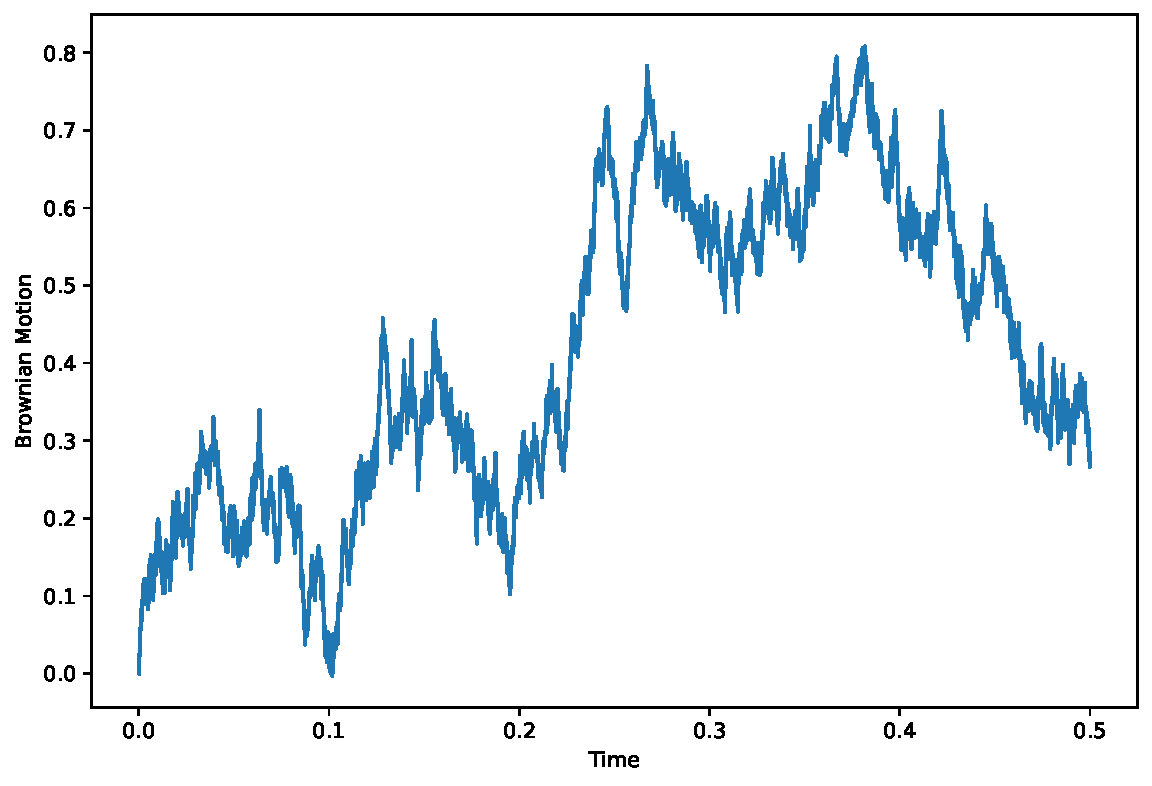
\includegraphics{Chapter3_files/figure-pdf/simulated-brownian-motion-output-2.pdf}

--\textgreater{}

\section{Quadratic Variation}\label{sec-s_quadraticvariation}

If we take a large number \(n\) of time steps in the simulation of the
preceding section, we will see the distinctive characteristic of a
Brownian motion: it jiggles rapidly, moving up and down in a very
erratic way. The name Brownian motion derives from the botanist Robert
Brown's observations of the erratic behavior of particles suspended in a
fluid. This has long been thought to be a reasonable model for the
behavior of a stock price.\\
The plot of other functions with which we may be familiar will be much
smoother. This is captured in the concept of quadratic variation.

Consider a discrete partition \[0=t_0 < t_1 < t_2 < \cdots < t_N=T\] of
the time interval \([0,T]\). Let \(B\) be a Brownian motion and
calculate the sum of squared changes
\[\sum_{i=1}^N [\Delta B(t_i)]^2\; ,\] where \(\Delta B(t_i)\) denotes
the change \(B(t_i)-B(t_{i-1}).\) If we consider finer partitions with
the length of each time interval \(t_i-t_{i-1}\) going to zero, the
limit of the sum is called the quadratic variation of the process.
\index{quadratic variation} For a Brownian motion, the quadratic
variation over an interval \([0,T]\) is equal to \(T\) with probability
one. Here is a plot of the quadratic variation. For large values of
\(n\), it is equal to \(t\).

\phantomsection\label{quadratic-variation}
\begin{Shaded}
\begin{Highlighting}[]
\CommentTok{\# quadratic variation}
\NormalTok{Q }\OperatorTok{=}\NormalTok{ np.zeros(shape }\OperatorTok{=}\NormalTok{ (n, m))}
\CommentTok{\# Generate dB\^{}2}
\NormalTok{Q }\OperatorTok{=}\NormalTok{ (Bt[}\DecValTok{1}\NormalTok{:n }\OperatorTok{+} \DecValTok{1}\NormalTok{] }\OperatorTok{{-}}\NormalTok{ Bt[}\DecValTok{0}\NormalTok{:n])}\OperatorTok{**}\DecValTok{2}

\CommentTok{\# Quadratic variation is the cumulative sum of dB\^{}2}
\NormalTok{QV }\OperatorTok{=}\NormalTok{ np.zeros(shape }\OperatorTok{=}\NormalTok{ (n }\OperatorTok{+} \DecValTok{1}\NormalTok{, m))}
\NormalTok{QV[}\DecValTok{1}\NormalTok{:] }\OperatorTok{=}\NormalTok{ Q.cumsum(axis }\OperatorTok{=} \DecValTok{0}\NormalTok{)}
\NormalTok{plt.figure(figsize}\OperatorTok{=}\NormalTok{(}\DecValTok{9}\NormalTok{,}\DecValTok{6}\NormalTok{))}
\NormalTok{plt.plot(t,QV[:,}\DecValTok{0}\NormalTok{])}
\NormalTok{plt.xlabel(}\StringTok{"Time"}\NormalTok{)}
\NormalTok{plt.ylabel(}\StringTok{"Quadratic Variation"}\NormalTok{)}
\end{Highlighting}
\end{Shaded}

\phantomsection\label{quadratic-variation-1}
\begin{verbatim}
Text(0, 0.5, 'Quadratic Variation')
\end{verbatim}

Quadratic Variation

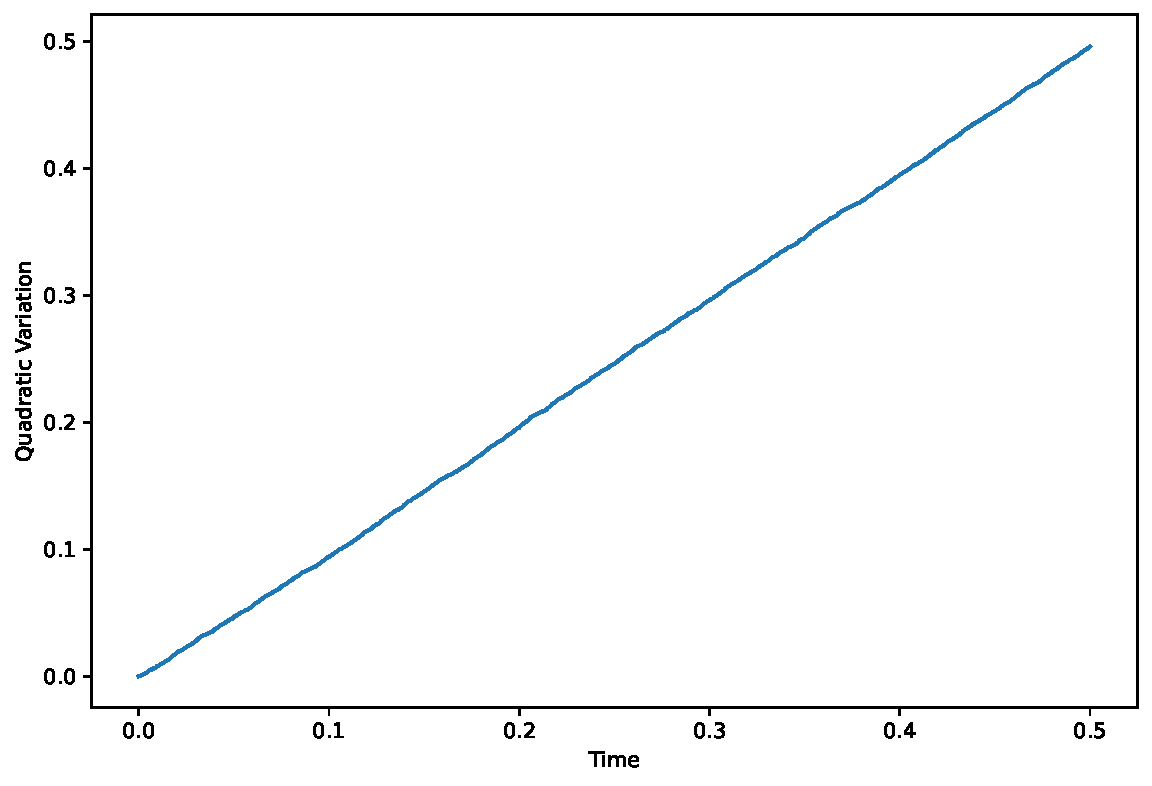
\includegraphics{Chapter3_files/figure-pdf/quadratic-variation-output-2.pdf}

The functions with which we are normally familiar are continuously
differentiable. If \(X\) is a continuously differentiable function of
time (in each state of the world), then the quadratic variation of \(X\)
will be zero. A simple example is a linear function: \(X(t) = at\) for
some constant \(a\). Then, taking \(t_i-t_{i-1} = \Delta t = T/N\) for
each \(i\), the sum of squared changes is
\[\sum_{i=1}^N [\Delta X(t_i)]^2 = \sum_{i=1}^N  [a\,\Delta t]^2 = Na^2 (\Delta t)^2 = Na^2 \left(\frac{T}{N}\right)^2 = \frac{a^2T^2}{N} \rightarrow 0\]
as \(N \rightarrow \infty\). Essentially the same argument shows that
the quadratic variation of any continuously differentiable function is
zero, because such a function is approximately linear at each point.
Below is a plot of the quadratic variation for the function \(X(t)=t\).
Look carefully at the scale of the y-axis

\begin{Shaded}
\begin{Highlighting}[]
\CommentTok{\# Plot dt\^{}2}
\NormalTok{plt.figure(figsize}\OperatorTok{=}\NormalTok{(}\DecValTok{9}\NormalTok{,}\DecValTok{6}\NormalTok{))}
\NormalTok{plt.plot(t,t }\OperatorTok{*}\NormalTok{ dt }\OperatorTok{**}\DecValTok{2}\NormalTok{)}
\end{Highlighting}
\end{Shaded}

\begin{figure}[H]

\caption{Approximate Squared Variation of \(f(t)=t\)}

{\centering 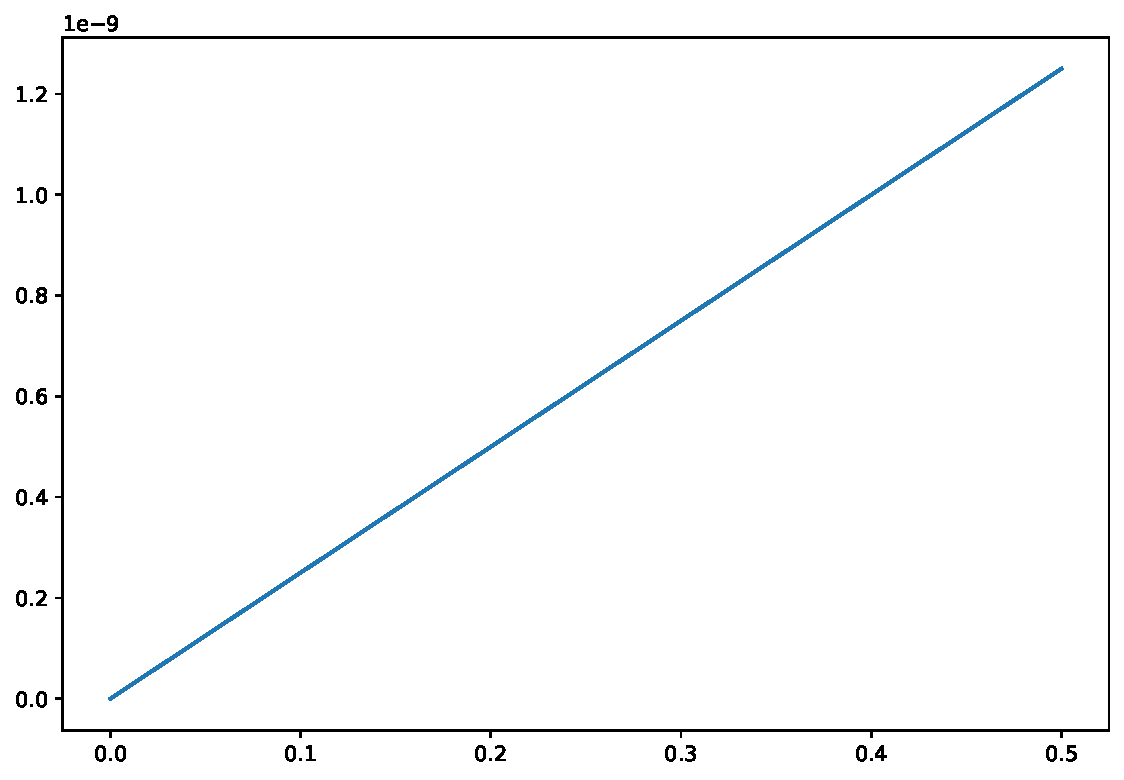
\includegraphics{Chapter3_files/figure-pdf/squaredvariation-output-1.pdf}

}

\end{figure}%

Thus, the jiggling of a Brownian motion, which leads to the nonzero
quadratic variation, is quite unusual. To explain exactly how unusual it
is, it is helpful to introduce the concept of total variation,
\index{total variation} which is defined in the same way as quadratic
variation but with the squared changes \([\Delta B(t_i)]^2\) replaced by
the absolute value of the changes \(|\Delta B(t_i)|.\) If the quadratic
variation of a continuous function is nonzero, then its total variation
is necessarily infinite, so each path of a Brownian motion has infinite
total variation (with probability one). It was mentioned above that,
with a large number of time steps in the simulation of the preceding
section, one could see the distinctive jiggling property of a Brownian
motion. This is not quite right. Any plot drawn by a pencil (or a laser
printer, for that matter) must have finite total variation, because the
total variation is the total distance traveled by the pencil. Hence, no
matter how many time steps one uses, one will never create a continuous
plot with the nonzero quadratic variation (and infinite total variation)
that a Brownian path has. Another way to understand this is to consider
focusing on a small segment of a plot and viewing it with a magnifying
glass. If the segment is small enough, and excluding the finite number
of kinks that a pencil can draw in the plot of a function, it will look
approximately like a straight line under the magnifying glass (with
slope equal to the derivative of the function). However, if one could
view a segment of a path of a true Brownian motion under a magnifying
glass, it would look much the same as the entire picture does to the
naked eye---no matter how small the segment, one would still see the
characteristic jiggling.

One may well question why we should be interested in this curious
mathematical object. The reason is that asset pricing inherently
involves martingales (variables that evolve randomly over time in such a
way that their expected changes are always zero), as our fundamental
pricing Equation~\ref{eq-formula} establishes. Furthermore, continuous
processes (variables whose paths are continuous functions of time) are
much more tractable mathematically than are processes that can jump at
some instants. More importantly, it is possible in a mathematical model
with continuous processes to define perfect hedges much more readily
than it is in a model involving jump processes. So, we are led to a
study of continuous martingales. An important fact is that any
non-constant continuous martingale must have infinite total variation!
So, the normal functions with which we are familiar are left behind once
we enter the study of continuous martingales.

There remains perhaps the question of why we focus on Brownian motion
within the world of continuous martingales. The answer here is that any
continuous martingale is really just a transformation of a Brownian
motion. This is a consequence of the following important fact, which is
known as Levy's theorem: \index{Levy's theorem}

\begin{tcolorbox}[enhanced jigsaw, leftrule=.75mm, colback=white, colframe=quarto-callout-tip-color-frame, breakable, title={Tip}, titlerule=0mm, bottomrule=.15mm, toprule=.15mm, arc=.35mm, left=2mm, toptitle=1mm, bottomtitle=1mm, rightrule=.15mm, colbacktitle=quarto-callout-tip-color!10!white, opacityback=0, coltitle=black, opacitybacktitle=0.6]

A continuous martingale is a Brownian motion if and only if its
quadratic variation over each interval \([0,T]\) equals \(T\).

\end{tcolorbox}

Thus, among continuous martingales, a Brownian motion is defined by the
condition that the quadratic variation over each interval \([0,T]\) is
equal to \(T\). This is really just a normalization. A different
continuous martingale may have a different quadratic variation, but it
can be converted to a Brownian motion just by deforming the time scale.
Furthermore, many continuous martingales can be constructed as
stochastic integrals with respect to a Brownian motion. We take up this
topic in the next section.

\section{Ito Processes}\label{sec-s_itoprocesses}

An Ito process is a variable \(X\) that changes over time as
\index{Ito process}
\begin{equation}\phantomsection\label{eq-itoprocess}{
\mathrm{d} X(t) = \mu(t)\,\mathrm{d} t+\sigma(t)\,\mathrm{d} B(t)\;,
}\end{equation}

where \(B\) is a Brownian motion, and \(\mu\) and \(\sigma\) can also be
random processes. Some regularity conditions are needed on \(\mu\) and
\(\sigma\) which we will omit, except for noting that \(\mu(t)\) and
\(\sigma(t)\) should be known at time \(t\). In particular, constant
\(\mu\) and \(\sigma\) are certainly acceptable. When we add the changes
over time, we get
\[X(T)=X(0) + \int_0^T\mu(t)\,\mathrm{d} t + \int_0^T\sigma(t)\,\mathrm{d} B(t)\]
for any \(T>0\). There are other types of random processes, in
particular, processes that can jump, but we will not consider them in
this book.

We will not formally define the integral
\(\int_0^T \sigma(t)\,\mathrm{d} B(t)\), but it should be understood as
being approximately equal to a discrete sum of the form
\[\sum_{i=1}^N \sigma(t_{i-1})\,\Delta B(t_i)\; ,\] where
\(0=t_0 < \cdots t_N=T\) and the time periods \(t_i-t_{i-1}\) are small.
Given that we can simulate the changes \(\Delta B(t_i)\) as random
normals, we can approximately simulate the random variable
\(\int_0^T \sigma(t)\,\mathrm{d} B(t)\) and hence we can approximately
simulate \(X(T)\).

An Ito process evolves continuously over time. We interpret
\(\mu(t)\,\mathrm{d} t\) as the expected change in \(X\) in an instant
\(\mathrm{d} t\). The quantity \(\mu(t)\) is also called the drift of
the process \(X\) at time \(t\). \index{drift} The coefficient
\(\sigma(t)\) is called the diffusion coefficient of \(X\) at time
\(t\). \index{diffusion coefficient}

If \(\mu\) and \(\sigma\) are constant, it is standard to refer to an
Ito process \(X\) as a \((\mu,\sigma)\)--Brownian motion. In this case
we have \[X(t)= \mu t + \sigma B_t\]

Of course, it is not a martingale when \(\mu\neq 0\). For example, when
\(\mu>0\), \(X\) tends to increase over time. However, it has the
jiggling property of a Brownian motion, scaled by the diffusion
coefficient \(\sigma\).

A very important fact is that an Ito process such as
Equation~\ref{eq-itoprocess} can be a martingale only if \(\mu=0\). This
should seem sensible, because \(\mu\,\mathrm{d} t\) is the expected
change in \(X\), and a process is a martingale only if its expected
change is zero.\footnote{If the sources of uncertainty in the market can
  be modeled as Brownian motions, then in fact every martingale is an
  Ito process with \(\mu=0\). This is some justification for the
  assumption we will make in this book, when studying continuous-time
  models, that all martingales are Ito processes.} This observation
plays a fundamental role in deriving asset pricing formulas, as we will
begin to see in Section~\ref{sec-s_girsanov}. Conversely, if \(\mu=0\)
and \begin{equation}\phantomsection\label{eq-regularity1}{
E \left[\int_0^T \sigma^2(t)\,\mathrm{d} t\right] < \infty
}\end{equation}

for each \(T\),\\
then the Ito process is a continuous martingale and the variance of its
date--\(T\) value, calculated with the information available at date 0,
is:
\[\mathrm{var}[X(T)] = E \left[\int_0^T \sigma^2(t)\,\mathrm{d} t\right]\; .\]

Whether \(\mu\) is zero or not, and independently of the assumption
Equation~\ref{eq-regularity1}, the quadratic variation of the Ito
process \(X\) is
\begin{equation}\phantomsection\label{eq-itoquadraticvariation}{
\lim_{N \rightarrow \infty} \sum_{i=1}^N[\Delta X(t_i)]^2 = \int_0^T \sigma^2(t)\,\mathrm{d} t
}\end{equation}

with probability one. Thus we obtain (when \(\mu=0\) and
Equation~\ref{eq-regularity1} holds) a continuous martingale with a
different quadratic variation than a Brownian motion via the diffusion
function \(\sigma\). In fact, when Equation~\ref{eq-regularity1} holds,
a somewhat more precise definition of the stochastic integral is the
(unique) martingale with quadratic variation given by
Equation~\ref{eq-itoquadraticvariation}.

To compute the quadratic variation of an Ito process, we use the
following simple and important rules (for the sake of brevity, we drop
the \((t)\) notation from \(B(t)\) here and sometimes later):

\begin{tcolorbox}[enhanced jigsaw, leftrule=.75mm, colback=white, colframe=quarto-callout-tip-color-frame, breakable, title={Tip}, titlerule=0mm, bottomrule=.15mm, toprule=.15mm, arc=.35mm, left=2mm, toptitle=1mm, bottomtitle=1mm, rightrule=.15mm, colbacktitle=quarto-callout-tip-color!10!white, opacityback=0, coltitle=black, opacitybacktitle=0.6]

\begin{equation}\phantomsection\label{eq-dtsquared}{
(\mathrm{d} t)^2 = 0\;, 
}\end{equation}

\begin{equation}\phantomsection\label{eq-dtdB}{
(\mathrm{d} t)(\mathrm{d} B) =0\;, 
}\end{equation}

\begin{equation}\phantomsection\label{eq-dBsquared}{
(\mathrm{d} B)^2 =\mathrm{d} t\;. 
}\end{equation}

\end{tcolorbox}

We apply these rules to compute the quadratic variation of \(X\) as
follows:

\begin{tcolorbox}[enhanced jigsaw, leftrule=.75mm, colback=white, colframe=quarto-callout-tip-color-frame, breakable, title={Tip}, titlerule=0mm, bottomrule=.15mm, toprule=.15mm, arc=.35mm, left=2mm, toptitle=1mm, bottomtitle=1mm, rightrule=.15mm, colbacktitle=quarto-callout-tip-color!10!white, opacityback=0, coltitle=black, opacitybacktitle=0.6]

If \(\mathrm{d} X = \mu\,\mathrm{d} t + \sigma\,\mathrm{d} B\) for a
Brownian motion \(B\), then \begin{align*}
(\mathrm{d} X)^2 &= (\mu\,\mathrm{d} t+\sigma\,\mathrm{d} B)^2\\
&= \mu^2(\mathrm{d} t)^2 + 2\mu\sigma(\mathrm{d} t)(\mathrm{d} B) + \sigma^2(\mathrm{d} B)^2\\
&= 0 + 0 + \sigma^2\,\mathrm{d} t\;.
\end{align*}

\end{tcolorbox}

We integrate this from 0 to \(T\) to obtain the quadratic variation
Equation~\ref{eq-itoquadraticvariation} over that time
period:\footnote{In a more formal mathematical presentation, one
  normally writes \(\mathrm{d}\langle X,X\rangle\) for what we are
  writing here as \((\mathrm{d} X)^2\). This is the differential of the
  quadratic variation process, and the quadratic variation through date
  \(T\) is \[
  \langle X,X\rangle (T) = \int_0^T \mathrm{d}\langle X,X\rangle(t) = \int_0^T \sigma^2(t)\,\mathrm{d} t\;.
  \]} \begin{equation}\phantomsection\label{eq-itoquadraticvariation2}{
\int_0^T (\mathrm{d} X(t))^2 = \int_0^T \sigma^2(t)\,\mathrm{d} t\;.
}\end{equation}

\section{Ito's Formula}\label{sec-s_itosformula}

First we recall some facts of the ordinary calculus. If \(y=g(x)\) and
\(x = f(t)\) with \(f\) and \(g\) being continuously differentiable
functions, then
\[\frac{\mathrm{d} y}{\mathrm{d} t} = \frac{\mathrm{d} y}{\mathrm{d} x}\times \frac{\mathrm{d} x}{\mathrm{d} t} = g'(x(t))f'(t)\; .\]
Over a time period \([0,T]\), this implies that
\[y(T) = y(0) + \int_0^T \frac{\mathrm{d} y}{\mathrm{d} t}\,\mathrm{d} t = y(0) + \int_0^T g'(x(t))f'(t)\,\mathrm{d} t\; .\]
Substituting \(\mathrm{d} x(t) = f'(t)\,\mathrm{d} t\), we can also
write this as
\begin{equation}\phantomsection\label{eq-ordinarycalculus}{
y(T) = y(0) + \int_0^T g'(x(t))\,\mathrm{d} x(t)\;.
}\end{equation}

We can contrast Equation~\ref{eq-ordinarycalculus} with a special case
of Ito's formula for the calculus of Ito processes (the more general
formula will be discussed in the next section). If \(B\) is a Brownian
motion and \(Y = g(B)\) for a twice-continuously differentiable function
\(g\), then \index{Ito's formula}
\begin{equation}\phantomsection\label{eq-itonew1}{
Y(T) = Y(0) + \int_0^T g'(B(t))\,\mathrm{d} B(t) + \frac{1}{2}\int_0^T g''(B(t))\,\mathrm{d} t\;.
}\end{equation}

Thus, relative to the ordinary calculus, Ito's formula has an extra term
involving the second derivative \(g''\). We can write
Equation~\ref{eq-itonew1} in differential form as
\[dY(t) = \frac{1}{2}g''(B(t))\,\mathrm{d} t + g'(B(t))\,\mathrm{d} B(t).\]
Thus, \(Y=g(B)\) is an Ito process with drift \(g''(B(t))/2\) and
diffusion coefficient \(g'(B(t))\).

To gain some intuition for the extra term in Ito's formula, we return to
the ordinary calculus. Given dates \(t<u\), the derivative defines a
linear approximation of the change in \(y\) over this time period; i.e.,
setting \(\Delta x = x(u)-x(t)\) and \(\Delta y = y(u) - y(t)\), we have
the approximation \[\Delta y \approx g'(x(t)) \,\Delta x\; .\] A better
approximation is given by the second-order Taylor series expansion
\[\Delta y \approx g'(x(t))\,\Delta x + \frac{1}{2} g''(x(t))\,[\Delta x]^2\; .\]
An interpretation of Equation~\ref{eq-ordinarycalculus} is that the
linear approximation works perfectly for infinitesimal time periods
\(\mathrm{d} t\), because we can compute the change in \(y\) over the
time period \([0,T]\) by summing up the infinitesimal changes
\(g'(x(t))\,\mathrm{d} x(t)\). In other words, the second-order term
\(\frac{1}{2} g''(x(t))\,[\Delta x]^2\) vanishes when we consider very
small time periods.

The second-order Taylor series expansion in the case of \(Y=g(B)\) is
\[\Delta Y \approx g'(B(t))\,\Delta B + \frac{1}{2} g''(B(t))\,[\Delta B]^2\; .\]
For example, given a partition \(0=t_0 < t_1 < \cdots < t_N=T\) of the
time interval \([0,T]\), we have, with the same notation we have used
earlier,

\[
Y(T) = Y(0) + \sum_{i=1}^N \Delta Y(t_i)  
\] \begin{equation}\phantomsection\label{eq-itonew2}{
\approx Y(0) + \sum_{i=1}^N g'(B(t_{i-1}))\,\Delta B(t_i) + \frac{1}{2} \sum_{i=1}^N g''(B(t_{i-1}))\,[\Delta B(t_i)]^2\;.
}\end{equation}

If we make the time intervals \(t_i-t_{i-1}\) shorter, letting
\(N \rightarrow \infty\), we cannot expect that the extra term here will
disappear, leading to the result Equation~\ref{eq-ordinarycalculus} of
the ordinary calculus, because we know that
\[\lim_{N \rightarrow \infty} \sum_{i=1}^N [\Delta B(t_i)]^2 = T\; ,\]
whereas for the continuously differentiable function \(x(t) = f(t)\),
the same limit is zero. In fact it seems sensible to interpret the limit
of \([\Delta B]^2\) as \((\mathrm{d} B)^2 =\mathrm{d} t\). This is
perfectly consistent with Ito's formula: if we take the limit in
Equation~\ref{eq-itonew2}, replacing the limit of \([\Delta B(t_i)]^2\)
with \((\mathrm{d} B)^2 = \mathrm{d} t\), we obtain
Equation~\ref{eq-itonew1}.

The code below defines a function \(g(x)=e^{x}\) (g'(x)=e\^{}x\$ and
g'\,'(x) = e\^{}x\$) and simulates the value \(e^{B_t}\) in two ways.
The first way is to simulate the Ito expansion
\[e^{B_t}=1 + \int_0^t e^{B_s} d B_s + \frac{1}{2}\int_0^t e^{B_s} ds\]
using the discretization
\[\Delta e^{B_t}= e^{B_t} \Delta B_t + \frac{1}{2} e^{B_t} \Delta t \]

\begin{Shaded}
\begin{Highlighting}[]
\CommentTok{\# Define a function and its first and second derivative}
\NormalTok{G }\OperatorTok{=} \KeywordTok{lambda}\NormalTok{ x: np.exp(x)}
\NormalTok{DG }\OperatorTok{=} \KeywordTok{lambda}\NormalTok{ x: np.exp(x)}
\NormalTok{DDG }\OperatorTok{=} \KeywordTok{lambda}\NormalTok{ x: np.exp(x)}
\CommentTok{\# Build G\textquotesingle{}(x)dB}
\NormalTok{GdB }\OperatorTok{=}\NormalTok{ np.zeros(shape }\OperatorTok{=}\NormalTok{ (n, m))}
\NormalTok{GdB[}\DecValTok{0}\NormalTok{] }\OperatorTok{=}\NormalTok{ np.repeat(DG(}\DecValTok{0}\NormalTok{), m) }\OperatorTok{*}\NormalTok{ inc[}\DecValTok{0}\NormalTok{]}
\NormalTok{GdB[}\DecValTok{1}\NormalTok{:] }\OperatorTok{=}\NormalTok{ DG(Bt[}\DecValTok{0}\NormalTok{:n }\OperatorTok{{-}} \DecValTok{1}\NormalTok{]) }\OperatorTok{*}\NormalTok{ inc[}\DecValTok{1}\NormalTok{:]}
\NormalTok{SI }\OperatorTok{=}\NormalTok{ np.zeros(shape }\OperatorTok{=}\NormalTok{ (n, m))}
\CommentTok{\# Stochastic Integral is cumulative sum of G\textquotesingle{}(B)dB plus initial}
\NormalTok{SI }\OperatorTok{=}\NormalTok{ GdB.cumsum(axis }\OperatorTok{=} \DecValTok{0}\NormalTok{) }\OperatorTok{+} \FloatTok{0.5} \OperatorTok{*}\NormalTok{ (DDG(Bt[}\DecValTok{0}\NormalTok{:n])}\OperatorTok{*}\NormalTok{Q).cumsum(axis }\OperatorTok{=}\DecValTok{0}\NormalTok{) }\OperatorTok{+}\NormalTok{ G(}\DecValTok{0}\NormalTok{)}
\CommentTok{\# Compare Ito\textquotesingle{}s Lemma }
\NormalTok{plt.figure(figsize}\OperatorTok{=}\NormalTok{(}\DecValTok{9}\NormalTok{,}\DecValTok{6}\NormalTok{))}
\NormalTok{plt.plot(t[}\DecValTok{0}\NormalTok{:n], SI[:,}\DecValTok{0}\NormalTok{])}
\end{Highlighting}
\end{Shaded}

\begin{figure}[H]

\caption{Simulated Ito Formula}

{\centering 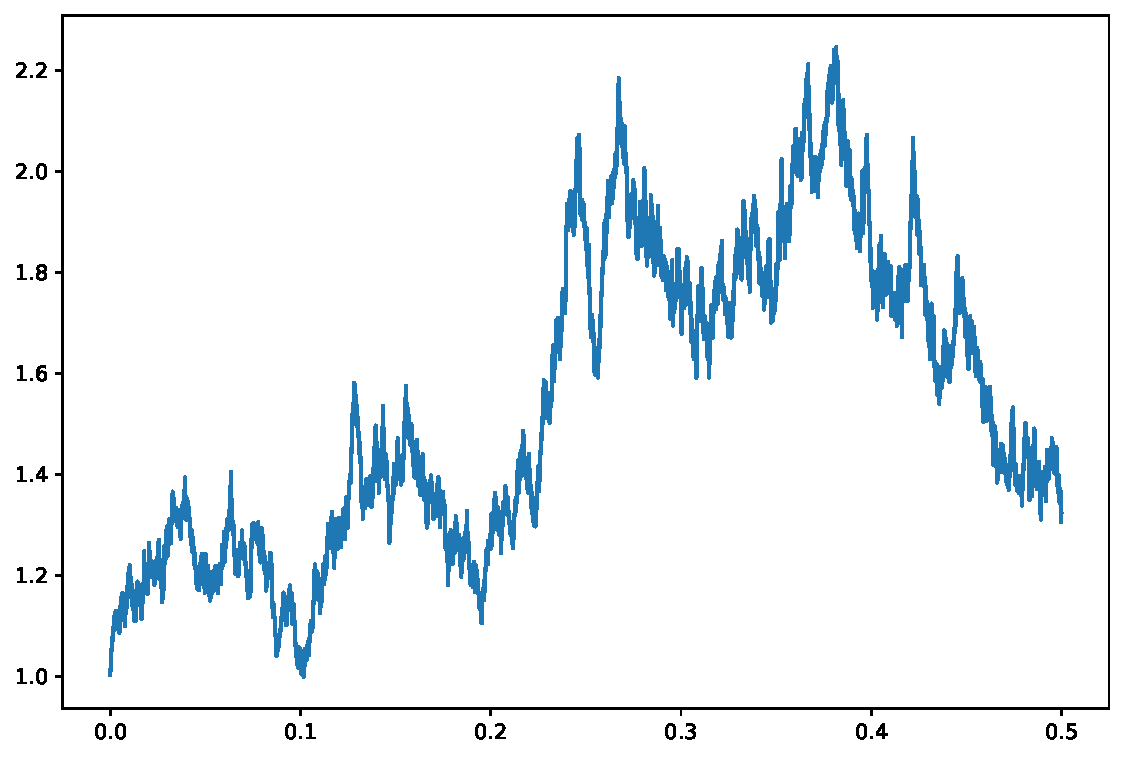
\includegraphics{Chapter3_files/figure-pdf/simulated-ito-formula-output-1.pdf}

}

\end{figure}%

Below is the exact simulated solution \(e^{B_t}\). It is almost
impossible to see a difference.

\begin{Shaded}
\begin{Highlighting}[]
\CommentTok{\#exact solution}
\NormalTok{plt.figure(figsize}\OperatorTok{=}\NormalTok{(}\DecValTok{9}\NormalTok{,}\DecValTok{6}\NormalTok{))}
\NormalTok{plt.plot(t[}\DecValTok{0}\NormalTok{:n], G(Bt[}\DecValTok{1}\NormalTok{:n }\OperatorTok{+} \DecValTok{1}\NormalTok{, }\DecValTok{0}\NormalTok{]))}
\end{Highlighting}
\end{Shaded}

\begin{figure}[H]

\caption{Simulated Exact Solution}

{\centering 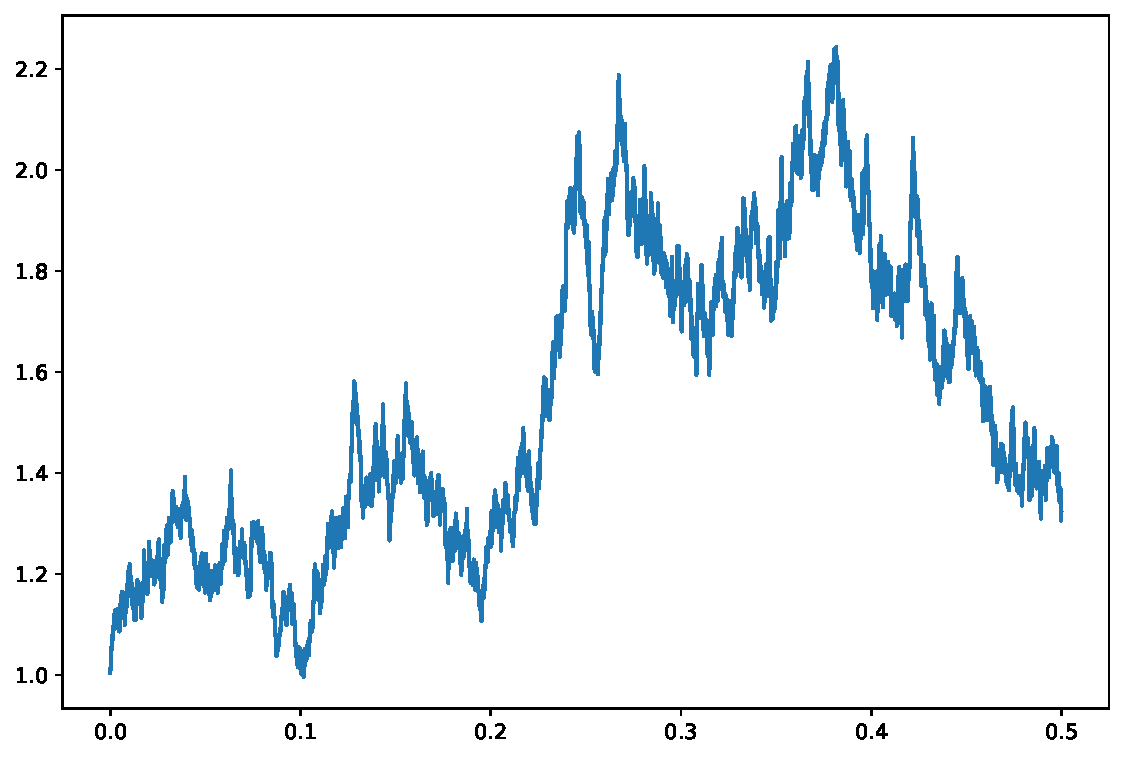
\includegraphics{Chapter3_files/figure-pdf/simulated-exact-solution-output-1.pdf}

}

\end{figure}%

Below we plot the \(\int_0^t \frac{1}{2} g''(B_s) ds\) term. Without
this term the two plots above will not match.

\begin{Shaded}
\begin{Highlighting}[]
\CommentTok{\# Correction term in Ito formula}
\NormalTok{QVV }\OperatorTok{=}\NormalTok{ np.zeros(shape }\OperatorTok{=}\NormalTok{ (n, m))}
\NormalTok{QVV }\OperatorTok{=} \FloatTok{0.5}\OperatorTok{*}\NormalTok{(DDG(Bt[}\DecValTok{0}\NormalTok{:n]) }\OperatorTok{*}\NormalTok{ Q).cumsum(axis }\OperatorTok{=} \DecValTok{0}\NormalTok{)}
\NormalTok{plt.figure(figsize}\OperatorTok{=}\NormalTok{(}\DecValTok{9}\NormalTok{,}\DecValTok{6}\NormalTok{))}
\NormalTok{plt.plot(t[}\DecValTok{0}\NormalTok{:n], QVV[:,}\DecValTok{0}\NormalTok{])}
\end{Highlighting}
\end{Shaded}

\begin{figure}[H]

\caption{Second Derivative Term in Ito's Formula}

{\centering 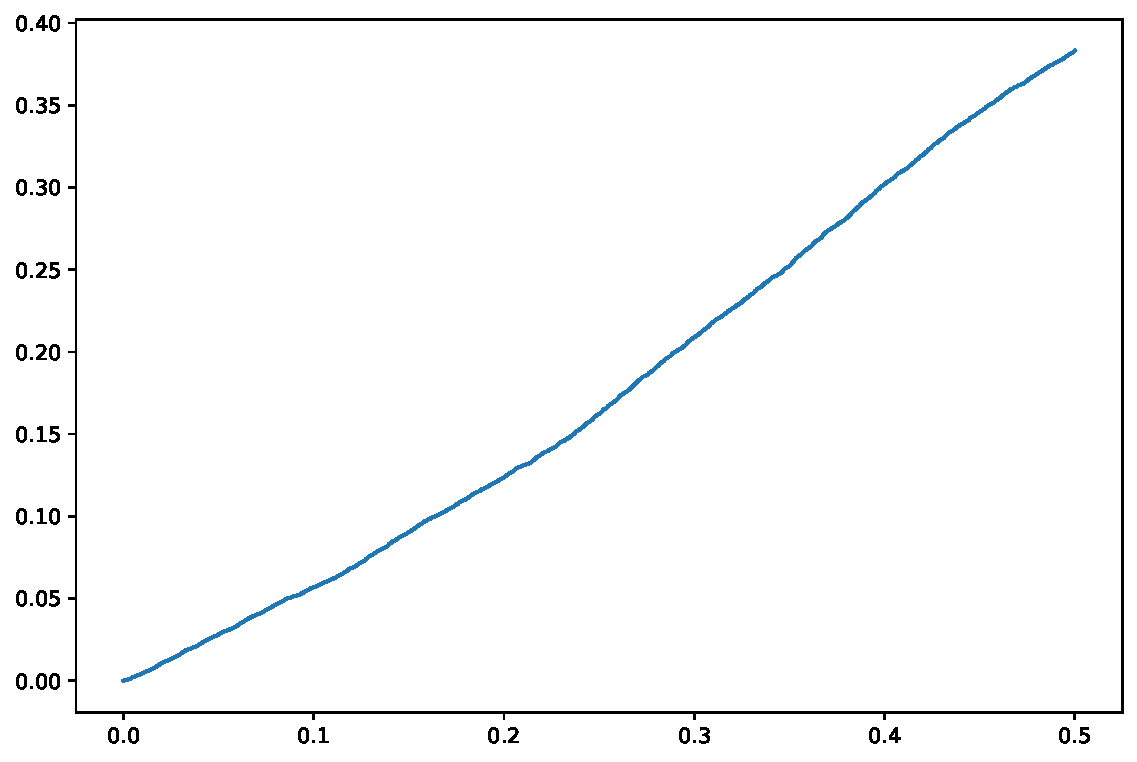
\includegraphics{Chapter3_files/figure-pdf/correction-output-1.pdf}

}

\end{figure}%

\section{Multiple Ito Processes}\label{multiple-ito-processes}

Now consider two Ito processes

\begin{equation}\phantomsection\label{eq-itoprocess110}{
\mathrm{d} X(t) = \mu_x(t)\,\mathrm{d} t + \sigma_x(t)\,\mathrm{d} B_x(t)\;,
}\end{equation}

\begin{equation}\phantomsection\label{eq-itoprocess111}{
\mathrm{d} Y(t) = \mu_y(t)\,\mathrm{d} t + \sigma_y(t)\,\mathrm{d} B_y(t)\;,
}\end{equation}

where \(B_x\) and \(B_y\) can be different Brownian motions. The
relation between the two Brownian motions is determined by their
covariance or correlation. Given dates \(t<u\), we know that both
changes \(B_x(u)-B_x(t)\) and \(B_y(u)-B_y(t)\) are normally distributed
with mean 0 and variance equal to \(u-t\). There will exist a (possibly
random) process \(\rho\) such that the covariance \index{covariance} of
these two normally distributed random variables, given the information
at date \(t\), is
\[E_t \left[\int_t^u \rho(s)\,\mathrm{d} s\right]\; .\] The process
\(\rho\) is called the correlation coefficient of the two Brownian
motions, \index{correlation coefficient} because when it is constant the
correlation of the changes \(B_x(u)-B_x(t)\) and \(B_y(u)-B_y(t)\) is
\[\frac{\text{covariance}}{\text{product of standard deviations}}  = \frac{\int_t^u \rho \,\mathrm{d} s}{\sqrt{u-t} \sqrt{u-t}} = \frac{(u-t)\rho}{u-t} = \rho\; .\]
Moreover, given increasingly fine partitions \(0=t_0 < \cdots < t_N=T\)
of an interval \([0,T]\) as before, we will have
\[\sum_{i=1}^N \Delta B_x(t_i) \times \Delta B_y(t_i) \rightarrow \int_0^T \rho(t)\,\mathrm{d} t\]
as \(N \rightarrow \infty\), with probability one.

We know that
\begin{equation}\phantomsection\label{eq-itoprocess112}{\sum _{i=1}^N [\Delta X(t_i)]^2 \rightarrow \int_0^T \sigma_x^2(t)\,\mathrm{d} t \quad \text{and}\quad  \sum _{i=1}^N [\Delta Y(t_i)]^2 \rightarrow \int_0^T\sigma_y^2(t)\,\mathrm{d} t\;.
}\end{equation}

Furthermore, it can be shown that the sum of products satisfies
\begin{equation}\phantomsection\label{eq-itoprocess113}{
\sum_{i=1}^N \Delta X(t_i) \times \Delta Y(t_i) \rightarrow \int_0^T \sigma_x(t)\sigma_y(t)\rho(t)\,\mathrm{d} t\;.
}\end{equation}

\begin{tcolorbox}[enhanced jigsaw, leftrule=.75mm, colback=white, colframe=quarto-callout-tip-color-frame, breakable, title={Tip}, titlerule=0mm, bottomrule=.15mm, toprule=.15mm, arc=.35mm, left=2mm, toptitle=1mm, bottomtitle=1mm, rightrule=.15mm, colbacktitle=quarto-callout-tip-color!10!white, opacityback=0, coltitle=black, opacitybacktitle=0.6]

By adding the rule \begin{equation}\phantomsection\label{eq-dBdB}{
(\mathrm{d} B_x)(\mathrm{d} B_y) = \rho\,\mathrm{d} t 
}\end{equation} to the rules
Equation~\ref{eq-dtsquared}--Equation~\ref{eq-dBsquared}, we can compute
the limit in Equation~\ref{eq-itoprocess113} as

\[
\lim_{N \rightarrow\infty} \sum_{i=1}^N \Delta X(t_i) \times \Delta Y(t_i)  = \int_0^T (\mathrm{d} X)(\mathrm{d} Y)
\] \[
= \int_0^T (\mu_x\,\mathrm{d} t +\sigma_x\,\mathrm{d} B_x)(\mu_y\,\mathrm{d} t+\sigma_y\,\mathrm{d} B_y)
\] \begin{equation}\phantomsection\label{eq-itojointvariation}{
= \int_0^T\sigma_x(t)\sigma_y(t) \rho(t)\,\mathrm{d} t\;.
}\end{equation}

\end{tcolorbox}

The most general case of Ito's formula that we will need is for a
function \(Z(t) = g(t, X(t), Y(t))\) where \(X\) and \(Y\) are Ito
processes as in Equation~\ref{eq-itoprocess110} -
Equation~\ref{eq-itoprocess111}. In this case, Ito's formula
is\footnote{We need to assume \(g(t,x,y)\) is continuously
  differentiable in \(t\) and twice continuously differentiable in
  \((x,y)\) for Equation~\ref{eq-itogeneralnew} and
  Equation~\ref{eq-itogeneralnew2} to be valid. Note also that we are
  using a short-hand notation here. The partial derivatives of \(g\)
  will generally depend on \(t\), \(X(t)\) and \(Y(t)\) just as \(g\)
  does.}

\[
Z(T) = Z(0) + \int_0^T \frac{\partial g}{\partial t}\,\mathrm{d} t + \int_0^T \frac{\partial g}{\partial x}\,\mathrm{d} X(t) + \int_0^T \frac{\partial g}{\partial y}\,\mathrm{d} Y(t) 
\] \[
+ \frac{1}{2} \int_0^T \frac{\partial^2 g}{\partial x^2}\,(\mathrm{d} X(t))^2 +  \frac{1}{2} \int_0^T \frac{\partial^2 g}{\partial y^2}\,(\mathrm{d} Y(t))^2 
\] \begin{equation}\phantomsection\label{eq-itogeneralnew}{
+  \int_0^T \frac{\partial^2 g}{\partial x\partial y}\,(\mathrm{d} X(t))( \mathrm{d} Y(t))\;.
}\end{equation}

In this equation, we apply the rules
Equation~\ref{eq-dtsquared}--Equation~\ref{eq-dBdB} to compute
\begin{align*}
(\mathrm{d} X(t))^2&= \sigma_x^2(t)\,\mathrm{d} t\; ,\\
(\mathrm{d} Y(t))^2 &= \sigma_y^2(t)\,\mathrm{d} t\; ,\\
(\mathrm{d} X(t))( \mathrm{d} Y(t)) &= \sigma_x(t)\sigma_y(t)\rho(t)\,\mathrm{d} t\;.
\end{align*} Ito's Equation~\ref{eq-itogeneralnew} appears a bit simpler
(and easier to remember) if we write it in differential form.'' We have:

\begin{tcolorbox}[enhanced jigsaw, leftrule=.75mm, colback=white, colframe=quarto-callout-tip-color-frame, breakable, title={Tip}, titlerule=0mm, bottomrule=.15mm, toprule=.15mm, arc=.35mm, left=2mm, toptitle=1mm, bottomtitle=1mm, rightrule=.15mm, colbacktitle=quarto-callout-tip-color!10!white, opacityback=0, coltitle=black, opacitybacktitle=0.6]

If \(Z(t) = g(t, X(t), Y(t))\) where \(X\) and \(Y\) are Ito processes
as in Equation~\ref{eq-itoprocess110} - Equation~\ref{eq-itoprocess111},
then

\[
\mathrm{d} Z =  \frac{\partial g}{\partial t}\,\mathrm{d} t + \frac{\partial g}{\partial x}\,\mathrm{d} X +  \frac{\partial g}{\partial y}\,\mathrm{d} Y + \frac{1}{2} \frac{\partial^2 g}{\partial x^2}\,(\mathrm{d} X)^2 +  \frac{1}{2}  \frac{\partial^2 g}{\partial y^2}\,(\mathrm{d} Y)^2 
\] \begin{equation}\phantomsection\label{eq-itogeneralnew2}{
+ \frac{\partial^2 g}{\partial x\partial y}\,(\mathrm{d} X)(\mathrm{d} Y)\;.
}\end{equation}

\end{tcolorbox}

\section{Examples of Ito's Formula}\label{sec-s_examples}

The following are the applications of Ito's formula that will be used
most frequently in the book. They follow from the boxed formula at the
end of the previous section by taking \(g(x,y)=xy\) or \(g(x,y)=y/x\) or
\(g(x)=e^x\) or \(g(x) = \log x\).

\begin{tcolorbox}[enhanced jigsaw, leftrule=.75mm, colback=white, colframe=quarto-callout-tip-color-frame, breakable, title={Tip}, titlerule=0mm, bottomrule=.15mm, toprule=.15mm, arc=.35mm, left=2mm, toptitle=1mm, bottomtitle=1mm, rightrule=.15mm, colbacktitle=quarto-callout-tip-color!10!white, opacityback=0, coltitle=black, opacitybacktitle=0.6]

\textbf{Products.}; If \(Z=XY\), then
\(\mathrm{d} Z=X\,\mathrm{d} Y+Y\,\mathrm{d} X + (\mathrm{d} X)(\mathrm{d} Y)\).
We can write this as \begin{equation}\phantomsection\label{eq-rule2}{
\frac{\mathrm{d} Z}{Z}=\frac{\mathrm{d} X}{X} + \frac{\mathrm{d} Y}{Y} + \left(\frac{\mathrm{d} X}{X}\right)\left(\frac{\mathrm{d} Y}{Y}\right)\;.
}\end{equation}

\end{tcolorbox}

\begin{tcolorbox}[enhanced jigsaw, leftrule=.75mm, colback=white, colframe=quarto-callout-tip-color-frame, breakable, title={Tip}, titlerule=0mm, bottomrule=.15mm, toprule=.15mm, arc=.35mm, left=2mm, toptitle=1mm, bottomtitle=1mm, rightrule=.15mm, colbacktitle=quarto-callout-tip-color!10!white, opacityback=0, coltitle=black, opacitybacktitle=0.6]

\textbf{Ratios.}; If \(Z=Y/X\), then
\begin{equation}\phantomsection\label{eq-rule4}{\frac{\mathrm{d} Z}{Z} = \frac{\mathrm{d} Y}{Y} -\frac{\mathrm{d} X}{X} - \left(\frac{\mathrm{d} Y}{Y}\right)\left(\frac{\mathrm{d} X}{X}\right) + \left(\frac{\mathrm{d} X}{X}\right)^2\;.
}\end{equation}

\end{tcolorbox}

\begin{tcolorbox}[enhanced jigsaw, leftrule=.75mm, colback=white, colframe=quarto-callout-tip-color-frame, breakable, title={Tip}, titlerule=0mm, bottomrule=.15mm, toprule=.15mm, arc=.35mm, left=2mm, toptitle=1mm, bottomtitle=1mm, rightrule=.15mm, colbacktitle=quarto-callout-tip-color!10!white, opacityback=0, coltitle=black, opacitybacktitle=0.6]

\textbf{Exponentials.}; If \(Z=\mathrm{e}^X\), then
\begin{equation}\phantomsection\label{eq-rule5}{\frac{\mathrm{d} Z}{Z}=\mathrm{d} X + \frac{(\mathrm{d} X)^2}{2}\;.
}\end{equation}

\end{tcolorbox}

\begin{tcolorbox}[enhanced jigsaw, leftrule=.75mm, colback=white, colframe=quarto-callout-tip-color-frame, breakable, title={Tip}, titlerule=0mm, bottomrule=.15mm, toprule=.15mm, arc=.35mm, left=2mm, toptitle=1mm, bottomtitle=1mm, rightrule=.15mm, colbacktitle=quarto-callout-tip-color!10!white, opacityback=0, coltitle=black, opacitybacktitle=0.6]

\textbf{Logarithms.}; If \(Z=\log X\), then
\begin{equation}\phantomsection\label{eq-rule6}{
\mathrm{d} Z=\frac{\mathrm{d} X}{X} - \frac{1}{2}\left(\frac{\mathrm{d} X}{X}\right)^2\;.
}\end{equation}

\end{tcolorbox}

\begin{tcolorbox}[enhanced jigsaw, leftrule=.75mm, colback=white, colframe=quarto-callout-tip-color-frame, breakable, title={Tip}, titlerule=0mm, bottomrule=.15mm, toprule=.15mm, arc=.35mm, left=2mm, toptitle=1mm, bottomtitle=1mm, rightrule=.15mm, colbacktitle=quarto-callout-tip-color!10!white, opacityback=0, coltitle=black, opacitybacktitle=0.6]

\textbf{Compounding/Discounting.} Let\\
\[Y(t) =\exp\left(\int_0^t q(s)\,\mathrm{d} s\right)\] for some
(possibly random) process \(q\) and define \(Z=XY\) for any Ito process
\(X\). The usual calculus gives us
\(\mathrm{d} Y(t)=q(t)Y(t)\,\mathrm{d} t\), and the product rule above
implies \begin{equation}\phantomsection\label{eq-compdisc1}{
\frac{\mathrm{d} Z}{Z}=q\,\mathrm{d} t + \frac{\mathrm{d} X}{X}\;.
}\end{equation}

This is the same as in the usual calculus.

\end{tcolorbox}

\section{Reinvesting Dividends}\label{sec-s_reinvestingdividends}

Frequently, we will assume that the asset underlying a derivative
security pays a constant dividend yield, \index{dividend yield} which we
will denote by \(q\). This means, for an asset with price \(S(t)\), that
the dividend in an instant \(\mathrm{d} t\) is \(q S(t)\,\mathrm{d} t\).
If the dividends are reinvested in new shares, the number of shares will
grow exponentially at rate \(q\). To see this, consider the portfolio
starting with a single share of the asset and reinvesting dividends
until some date \(T\). Let \(X(t)\) denote the number of shares
resulting from this strategy at any time \(t\leq T\). Then the dividend
received at date \(t\) is \(q S(t)X(t)\,\mathrm{d} t\), which can be
used to purchase \(q X(t)\,\mathrm{d} t\) new shares. This implies that
\(\mathrm{d} X(t)=q X(t)\,\mathrm{d} t\), or
\(\mathrm{d} X(t)/\mathrm{d} t = q X(t)\), and it is easy to check (and
very well known) that this equation is solved by
\(X(t)=\mathrm{e}^{q t}X(0)\). In our case, with \(X(0)=1\), we have
\(X(t)=\mathrm{e}^{q t}\).

The dollar value of the trading strategy just described will be
\(X(t)S(t) = \mathrm{e}^{q t}S(t)\). Denote this by \(V(t)\). This is
the value of a non-dividend-paying portfolio, because all dividends are
reinvested. From the Compounding/Discounting example in
Section~\ref{sec-s_examples}, we know that
\begin{equation}\phantomsection\label{eq-reinvestingdividends}{ 
\frac{\mathrm{d} V}{V} = q\,\mathrm{d} t + \frac{\mathrm{d} S}{S}\;.
}\end{equation}

This means that the rate of return on the portfolio is the dividend
yield \(q\,\mathrm{d} t\) plus the return \(\mathrm{d} S/S\) due to
capital gains.

\section{Geometric Brownian Motion}\label{sec-s_geometricbrownianmotion}

A random variable is lognormally distributed if it can be written as
\(\tilde{y}=  e^{\tilde{x}}\) where \(\tilde{x}\) is distributed
according to a normal distribution with mean \(m\) and standard
deviation \(s\). The expected value of \(\tilde{y}\) is given by
\(E[\tilde{y}] = e^{m+\frac{s^2}{2}}\).

\begin{tcolorbox}[enhanced jigsaw, leftrule=.75mm, colback=white, colframe=quarto-callout-tip-color-frame, breakable, title={Tip}, titlerule=0mm, bottomrule=.15mm, toprule=.15mm, arc=.35mm, left=2mm, toptitle=1mm, bottomtitle=1mm, rightrule=.15mm, colbacktitle=quarto-callout-tip-color!10!white, opacityback=0, coltitle=black, opacitybacktitle=0.6]

\textbf{Lognormal Random Variable.}; If \(\tilde{x}\) is normally
distributed with mean \(m\) and standard deviation \(s\), then
\(e^{\tilde{x}}\) is lognormally distributed and
\begin{equation}\phantomsection\label{eq-lognormal}{E[e^{\tilde{x}}]=e^{m + \frac{1}{2} s^2};.
}\end{equation}

\end{tcolorbox}

An important stochastic process is the Geometric Brownian Motion given
by \begin{equation}\phantomsection\label{eq-exponential1}{
S(t)=S(0)\exp\left(\mu t- \sigma^2 t/2 + \sigma B(t)\right)
}\end{equation}

for constants \(\mu\) and \(\sigma\), where \(B\) is a Brownian motion.
Note that for each time \(t\), geometric Brownian motion is a lognormal
random variable. Using the product rule and the rule for exponentials,
we obtain \begin{equation}\phantomsection\label{eq-Y}{
\frac{\mathrm{d} S}{S} = \mu\,\mathrm{d} t+\sigma\,\mathrm{d} B\;.
}\end{equation}

When we see an equation of the form Equation~\ref{eq-Y}, we should
recognize Equation~\ref{eq-exponential1} as the solution.

The process \(S\) is called a geometric Brownian motion.
\index{geometric Brownian motion} In keeping with the discussion of
Section~\ref{sec-s_itoprocesses}, we interpret Equation~\ref{eq-Y} as
stating that \(\mu\,\mathrm{d} t\) is the expected rate of change of
\(S\) and \(\sigma^2\,\mathrm{d} t\) is the variance of the rate of
change in an instant \(\mathrm{d} t\). We call \(\mu\) the drift and
\(\sigma\) the volatility. \index{volatility} The geometric Brownian
motion will grow at the average rate of \(\mu\), in the sense that
\(E[S(t)] = \mathrm{e}^{\mu t}S(0)\); one way to verify this uses the
formula for the mean of a lognormal random variable.

Taking the natural logarithm of Equation~\ref{eq-exponential1} gives an
equivalent form of the solution:
\begin{equation}\phantomsection\label{eq-exponential2}{
\log S(t)= \log S(0)+\left(\mu -\frac{1}{2}\sigma^2\right)t + \sigma B(t)\;.
}\end{equation} This shows that \(\log S(t) - \log S(0)\) is a
\((\mu-\sigma^2/2,\sigma)\)--Brownian motion. Given information at time
\(t\), the logarithm of \(S(u)\) for \(u>t\) is normally
\index{lognormal distribution}distributed with mean
\((u-t)(\mu-\sigma^2/2)\) and variance \((u-t)\sigma^2\). Because \(S\)
is the exponential of its logarithm, \(S\) can never be negative. For
this reason, a geometric Brownian motion is a better model for stock
prices than is a Brownian motion.

The differential of Equation~\ref{eq-exponential2} is
\begin{equation}\phantomsection\label{eq-exponential3}{
\mathrm{d} \log S(t) = \left(\mu -\frac{1}{2}\sigma^2\right)\,\mathrm{d} t+ \sigma\,\mathrm{d} B(t)\;.
}\end{equation}

We conclude:

\begin{tcolorbox}[enhanced jigsaw, leftrule=.75mm, colback=white, colframe=quarto-callout-tip-color-frame, breakable, title={Tip}, titlerule=0mm, bottomrule=.15mm, toprule=.15mm, arc=.35mm, left=2mm, toptitle=1mm, bottomtitle=1mm, rightrule=.15mm, colbacktitle=quarto-callout-tip-color!10!white, opacityback=0, coltitle=black, opacitybacktitle=0.6]

The equation
\[\frac{\mathrm{d} S}{S} = \mu\,\mathrm{d} t+\sigma\,\mathrm{d} B\] is
equivalent to the equation
\[\mathrm{d} \log S(t) = \left(\mu -\frac{1}{2}\sigma^2\right)\,\mathrm{d} t+ \sigma\,\mathrm{d} B(t)\; .\]
The solution of both equations is Equation~\ref{eq-exponential1} or the
equivalent Equation~\ref{eq-exponential2}.

\end{tcolorbox}

Over a discrete time interval \(\Delta t\),
Equation~\ref{eq-exponential3} implies that the change in the logarithm
of \(S\) is \begin{equation}\phantomsection\label{eq-exponential11}{
\Delta \log S = \left(\mu -\frac{1}{2}\sigma^2\right)\Delta t+ \sigma\,\Delta B\;.
}\end{equation}

If \(S\) is the price of a non-dividend-paying asset, then over the time
period \(t_{i-1}\) to \(t_i\), with \(t_i-t_{i-1}=\Delta t\), we have
\begin{equation}\phantomsection\label{eq-exponential10}{
\Delta \log S = r_i\,\Delta t\;,
}\end{equation}

where \(r_i\) is the continuously compounded annualized rate of return
\index{continuously compounded return} during the period \(\Delta t\).
This follows from the definition of the continuously compounded rate of
return as the constant rate over the time period \(\Delta t\) that would
cause \(S\) to grow (or fall) from \(S(t_{i-1})\) to \(S(t_i)\). To be
precise, \(r_i\) is defined by
\[\frac{S(t_i)}{S(t_{i-1})} = \mathrm{e}^{r_i\Delta t}\; ,\] which is
equivalent to Equation~\ref{eq-exponential10}. Thus, the geometric
Brownian motion model Equation~\ref{eq-Y} implies that the continuously
compounded annualized rate of return over a period of length
\(\Delta t\) is given by
\[r_i = \mu -\frac{1}{2}\sigma^2+ \frac{\sigma\Delta B}{\Delta t}\; .\]
This means that \(r_i\) is normally distributed with mean
\(\mu-\sigma^2/2\) and variance \(\sigma^2/\Delta t\). Given historical
data on the rates of return, the parameters \(\mu\) and \(\sigma\) can
be estimated by standard methods (see
Chapter~\ref{sec-c_stochasticvolatility}).

We can simulate a path of \(S\) by simulating the changes
\(\Delta \log S\). The random variable \(\sigma \Delta B\) in
Equation~\ref{eq-exponential11} has a normal distribution with zero mean
and variance equal to \(\sigma^2\Delta t\). We simulate it as
\(\sigma\sqrt{\Delta t}\) multiplied by a standard normal. The code
below simulates \(n=10000\) paths with \(m=1000\) time steps. There are
some features of the simulation which will prove useful later. The drift
\(\mu\) is labelled the interest rate \(r=0.1\). Other parameters are
\(\sigma = 0.2\), and \(T=0.5\). The drift of the log stock price is
labelled \(drift=r-\frac{\sigma^2}{2}\). The plot output is one of the
simulated sample paths. In practice, if we are only interested in the
terminal value of the stock price we would use many fewer subdivisions,
\(n=1\). Given a simulated mean zero normal random variable, \(z\),
changing the sign to \(-z\) is also a simulated normal random variable
with zero mean and the same standard deviation. As a result, we have two
simulations for the stock price labelled \(St\) and \(St1\), but we only
plot one sample path for \(St\).

\begin{Shaded}
\begin{Highlighting}[]
\CommentTok{\# Simulate Geometric Brownian Motion}
\ImportTok{import}\NormalTok{ numpy }\ImportTok{as}\NormalTok{ np}
\ImportTok{import}\NormalTok{ matplotlib.pyplot }\ImportTok{as}\NormalTok{ plt}
\CommentTok{\# number of paths}
\NormalTok{n }\OperatorTok{=} \DecValTok{10000}
\CommentTok{\#number of divisions}
\NormalTok{m }\OperatorTok{=} \DecValTok{1000}
\CommentTok{\# Interest rate (We set the drift equal to the interest rate)}
\NormalTok{r }\OperatorTok{=} \FloatTok{0.1}
\CommentTok{\# Volatility}
\NormalTok{sig }\OperatorTok{=} \FloatTok{0.2}
\CommentTok{\# Initial Stock Price}
\NormalTok{S0 }\OperatorTok{=} \DecValTok{42}
\CommentTok{\# Maturity}
\NormalTok{T }\OperatorTok{=} \FloatTok{0.5}
\CommentTok{\# Delta t}
\NormalTok{dt }\OperatorTok{=}\NormalTok{ T}\OperatorTok{/}\NormalTok{m}
\CommentTok{\# Drift}
\NormalTok{drift }\OperatorTok{=}\NormalTok{ (r}\OperatorTok{{-}}\FloatTok{0.5}\OperatorTok{*}\NormalTok{sig}\OperatorTok{**}\DecValTok{2}\NormalTok{)}
\CommentTok{\# Volatility}
\NormalTok{vol }\OperatorTok{=}\NormalTok{ sig }\OperatorTok{*}\NormalTok{ np.sqrt(dt)}

\NormalTok{t }\OperatorTok{=}\NormalTok{ np.array(}\BuiltInTok{range}\NormalTok{(}\DecValTok{0}\NormalTok{,m }\OperatorTok{+} \DecValTok{1}\NormalTok{,}\DecValTok{1}\NormalTok{)) }\OperatorTok{*}\NormalTok{ dt}

\CommentTok{\# seed for random generator}
\NormalTok{seed}\OperatorTok{=} \DecValTok{2020}
\CommentTok{\# define a random generator}
\NormalTok{np.random.seed(seed)}
\NormalTok{inc }\OperatorTok{=}\NormalTok{ np.zeros(shape }\OperatorTok{=}\NormalTok{ (m }\OperatorTok{+} \DecValTok{1}\NormalTok{, n))}
\NormalTok{inc[}\DecValTok{1}\NormalTok{:] }\OperatorTok{=}\NormalTok{ np.transpose(np.random.normal(loc }\OperatorTok{=} \DecValTok{0}\NormalTok{, scale }\OperatorTok{=}\NormalTok{ vol,size }\OperatorTok{=}\NormalTok{ (n,m)))}
\NormalTok{St }\OperatorTok{=}\NormalTok{ np.zeros(shape }\OperatorTok{=}\NormalTok{ (m }\OperatorTok{+} \DecValTok{1}\NormalTok{, n))}
\NormalTok{St }\OperatorTok{=}\NormalTok{ S0 }\OperatorTok{*}\NormalTok{ np.exp(np.cumsum(inc,axis}\OperatorTok{=}\DecValTok{0}\NormalTok{) }\OperatorTok{+}\NormalTok{ (drift }\OperatorTok{*}\NormalTok{ t[}\DecValTok{0}\NormalTok{:m }\OperatorTok{+} \DecValTok{1}\NormalTok{])[:,}\VariableTok{None}\NormalTok{])}
\NormalTok{St1 }\OperatorTok{=}\NormalTok{ S0 }\OperatorTok{*}\NormalTok{ np.exp(}\OperatorTok{{-}}\NormalTok{np.cumsum(inc,axis}\OperatorTok{=}\DecValTok{0}\NormalTok{) }\OperatorTok{+}\NormalTok{ (drift }\OperatorTok{*}\NormalTok{ t[}\DecValTok{0}\NormalTok{:m }\OperatorTok{+} \DecValTok{1}\NormalTok{])[:,}\VariableTok{None}\NormalTok{])}
\NormalTok{plt.figure(figsize}\OperatorTok{=}\NormalTok{(}\DecValTok{9}\NormalTok{,}\DecValTok{6}\NormalTok{))}
\NormalTok{plt.plot(t,St[:,}\DecValTok{1}\NormalTok{])}
\end{Highlighting}
\end{Shaded}

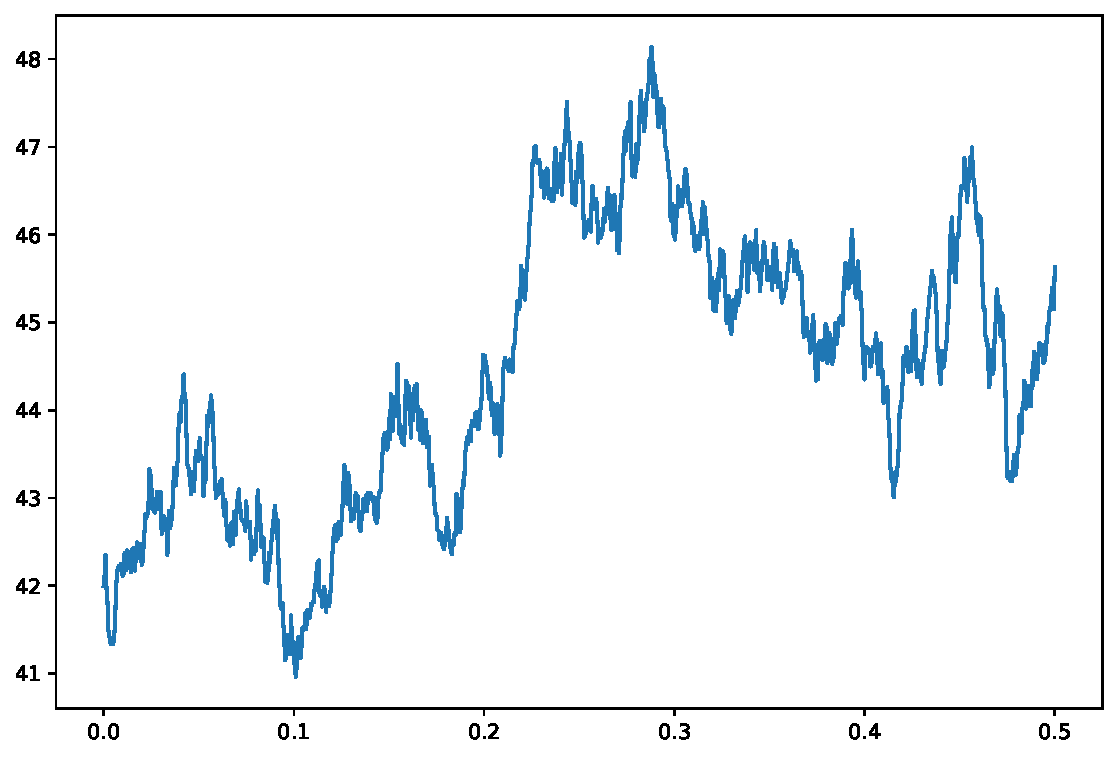
\includegraphics{Chapter3_files/figure-pdf/cell-9-output-1.pdf}

The plot below is the distribution of the simulated stock price at
\(T\).

\begin{Shaded}
\begin{Highlighting}[]
\NormalTok{plt.figure(figsize}\OperatorTok{=}\NormalTok{(}\DecValTok{9}\NormalTok{,}\DecValTok{6}\NormalTok{))}
\NormalTok{a}\OperatorTok{=}\NormalTok{plt.hist(St[m,:], bins}\OperatorTok{=}\DecValTok{100}\NormalTok{)}
\end{Highlighting}
\end{Shaded}

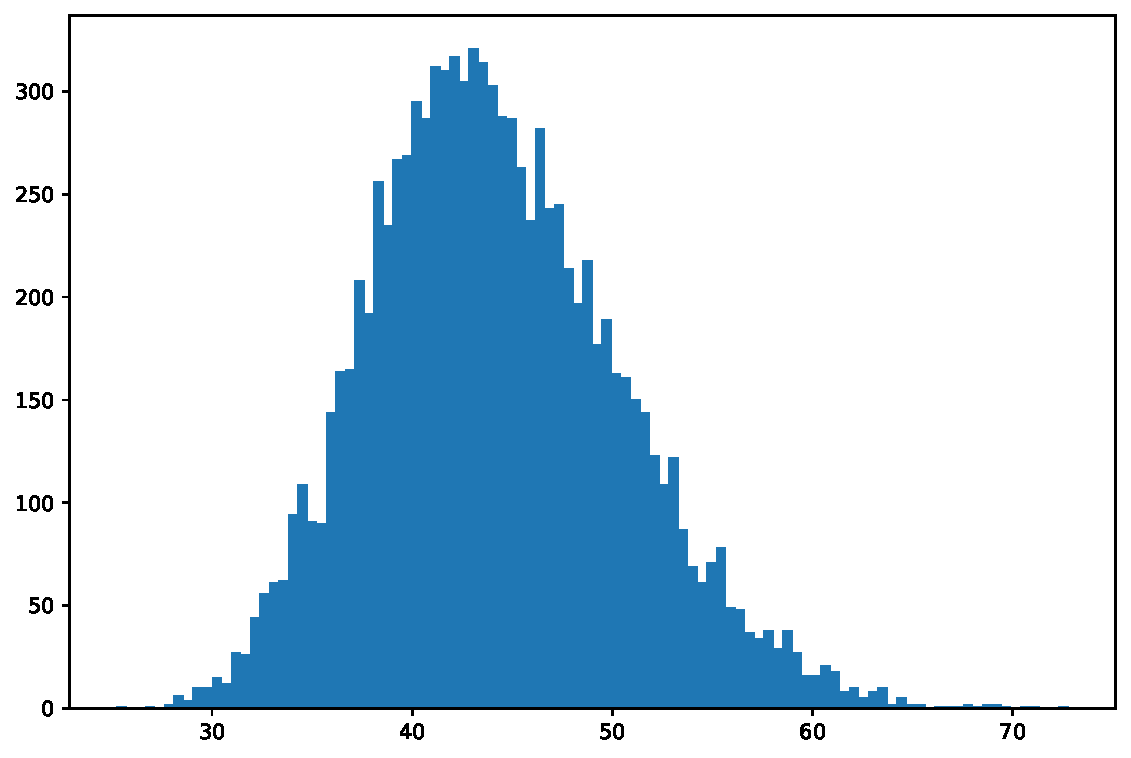
\includegraphics{Chapter3_files/figure-pdf/cell-10-output-1.pdf}

While Geometric Brownian Motion is an important stochastic process to
model stock prices, the process with drift equal to zero given by
\[X(t) = \exp\left(-\frac{\kappa^2}{2} + \kappa B_t\right)\]

satisfies \(E[X(t)]=1\) and \(E[X(t)|X(s)]=X(s)\) and is an important
example of a strictly positive martingale. Again, these facts can be
verified using the formula for the expected value of a lognormal random
variable. Notice we can write \[dX(t)= \kappa X(t) dB_t\] which agrees
with the martingale characterization of \(\int_0^t \sigma(X_t,t) dB_t\).

\section{Numeraires and Probabilities}\label{sec-s_girsanov}

When we change probability measures, we cannot expect a process \(B\)
that was a Brownian motion to remain a Brownian motion. The expected
change in a Brownian motion must always be zero, but when we change
probabilities, the expected change of \(B\) is likely to become nonzero.
(Likewise, a martingale is unlikely to remain a martingale when we
change probabilities.) However, the Brownian motion \(B\) will still be
an Ito process under the new probability measure. In fact, every Ito
process under one probability measure will still be an Ito process under
the new probability measure, and the diffusion coefficient of the Ito
process will be unaffected by the change in probabilities.\footnote{To
  be a little more precise, this is true provided sets of states of the
  world having zero probability continue to have zero probability when
  the probabilities are changed. Because of the way we change
  probability measures when we change numeraires (cf.
  Equation~\ref{eq-probSnumeraire}) this will always be true for us.}
Changing probabilities only changes the drift of an Ito process.

In a sense, this should not be surprising. It was noted in
Section~\ref{sec-s_quadraticvariation} that a Brownian motion \(B\) can
be defined as a continuous martingale with paths that jiggle in such a
way that the quadratic variation over any interval \([0,T]\) is equal to
\(T\). Changing the probabilities will change the probabilities of the
various paths (so it may affect the expected change in \(B\)) but it
will not affect how each path jiggles. So, under the new probability
measure, \(B\) should still be like a Brownian motion but it may have a
nonzero drift. If we consider a general Ito process, the reasoning is
the same. The diffusion coefficient \(\sigma\) determines how much each
path jiggles, and this is unaffected by changing the probability
measure. Furthermore, instantaneous covariances---the
\((\mathrm{d} X)(\mathrm{d} Y)\) terms---between Ito processes are
unaffected by changing the probability measure. Only the drifts are
affected.

As explained in Section~\ref{sec-s_introoptions}, we need to know the
distribution of the underlying under probability measures corresponding
to different numeraires. Let \(S\) be the price of an asset that has a
constant dividend yield \(q\), and, as in
Section~\ref{sec-s_reinvestingdividends}, let
\(V(t)=\mathrm{e}^{qt}S(t)\). This is the price of the portfolio in
which all dividends are reinvested, and we have
\[\frac{\mathrm{d} V}{V} = q\,\mathrm{d} t + \frac{\mathrm{d} S}{S}\; .\]
Let \(Y\) be the price of another another asset that does not pay
dividends. Let \(r(t)\) denote the instantaneous risk-free rate at date
\(t\) and let \(R(t) = \exp\left(\int_0^t r(s)\,\mathrm{d} s\right)\).
Assume \begin{align*}
 \frac{\mathrm{d} S}{S} &= \mu_s\,\mathrm{d} t+\sigma_s\,\mathrm{d} B_s\; ,\\
 \frac{\mathrm{d} Y}{Y} &= \mu_y\,\mathrm{d} t+\sigma_y\,\mathrm{d} B_y\;,
\end{align*} where \(B_s\) and \(B_y\) are Brownian motions under the
actual probability measure with correlation \(\rho\), and where
\(\mu_s, \mu_y, \sigma_s, \sigma_y\) and \(\rho\) can be quite general
random pro-cesses.\\
We consider the dynamics of the asset price \(S\) under three different
probability measures. In each case, we follow the same steps: (i) we
note that the ratio of an asset price to the numeraire asset price must
be a martingale, (ii) we use Ito's formula to calculate the drift of
this ratio, and (iii) we use the fact that the drift of a martingale
must be zero to compute the drift of \(\mathrm{d} S/S\).

\subsection{Risk-Neutral
Probabilities}\label{risk-neutral-probabilities}

Under the risk-neutral measure, \(Z(t)\) defined as
\[Z(t) = \frac{V(t)}{R(t)} = \exp\left(-\int_0^t r(s)\,\mathrm{d} s\right)V(t)\]
is a martingale. Using the compounding/discounting rule, we have
\[\frac{\mathrm{d} Z}{Z} =-r\,\mathrm{d} t + \frac{\mathrm{d} V}{V} = (q-r)\,\mathrm{d} t + \frac{\mathrm{d} S}{S}\; .\]
For \(Z\) to be a martingale, the drift (\(\mathrm{d} t\) part) of
\(\mathrm{d} Z/Z\) must be zero. Therefore, the drift of
\(\mathrm{d} S/S\) must be \((r-q)\,\mathrm{d} t\) under the
risk-neutral measure. Because the change of measure does not affect the
volatility, this implies:

\begin{tcolorbox}[enhanced jigsaw, leftrule=.75mm, colback=white, colframe=quarto-callout-tip-color-frame, breakable, title={Tip}, titlerule=0mm, bottomrule=.15mm, toprule=.15mm, arc=.35mm, left=2mm, toptitle=1mm, bottomtitle=1mm, rightrule=.15mm, colbacktitle=quarto-callout-tip-color!10!white, opacityback=0, coltitle=black, opacitybacktitle=0.6]

\begin{equation}\phantomsection\label{eq-riskneutral11}{
\frac{\mathrm{d} S}{S} =( r-q)\,\mathrm{d} t+\sigma_s\,\mathrm{d} B^*_s\;,
}\end{equation}

where \(B^*_s\) is a Brownian motion under the risk-neutral measure.

\end{tcolorbox}

\subsection{Underlying as the
Numeraire}\label{underlying-as-the-numeraire}

When \(V\) is the numeraire, the process \(Z(t)\) defined as
\[Z(t) = \frac{R(t)}{V(t)} = \frac{\exp\left(\int_0^t r(s)\,\mathrm{d} s\right)}{V(t)}\]
is a martingale. Using the rule for ratios, we have
\[\frac{\mathrm{d} Z}{Z} =r\,\mathrm{d} t - \frac{\mathrm{d} V}{V} + \left(\frac{\mathrm{d} V}{V}\right)^2 = (r -q+ \sigma^2_s)\,\mathrm{d} t - \frac{\mathrm{d} S}{S}\; .\]
Because the drift of \(\mathrm{d} Z/Z\) must be zero, this implies that
the drift of \(\mathrm{d} S/
S\) is \((r -q + \sigma^2_s)\,\mathrm{d} t\). We conclude that:

\begin{tcolorbox}[enhanced jigsaw, leftrule=.75mm, colback=white, colframe=quarto-callout-tip-color-frame, breakable, title={Tip}, titlerule=0mm, bottomrule=.15mm, toprule=.15mm, arc=.35mm, left=2mm, toptitle=1mm, bottomtitle=1mm, rightrule=.15mm, colbacktitle=quarto-callout-tip-color!10!white, opacityback=0, coltitle=black, opacitybacktitle=0.6]

\begin{equation}\phantomsection\label{eq-own11}{
\frac{\mathrm{d} S}{S} = (r-q+ \sigma^2_s)\,\mathrm{d} t+\sigma_s\,\mathrm{d} B^*_s\;,
}\end{equation}

where now \(B^*_s\) denotes a Brownian motion when
\(V(t)=\mathrm{e}^{qt}S(t)\) is the numeraire.

\end{tcolorbox}

\subsection{Another Risky Asset as the
Numeraire}\label{another-risky-asset-as-the-numeraire}

When \(Y\) is the numeraire, \(Z(t)\) defined as
\[Z(t) = \frac{V(t)}{Y(t)}\] must be a martingale. Using again the rule
for ratios, we have \begin{align*}
\frac{\mathrm{d} Z}{Z} &= \frac{\mathrm{d} V}{V} -\frac{\mathrm{d} Y}{Y}- \left(\frac{\mathrm{d} V}{V}\right)\left(\frac{\mathrm{d} Y}{Y}\right) + \left(\frac{\mathrm{d} Y}{Y}\right)^2\\
& = \frac{\mathrm{d} V}{V} -\frac{\mathrm{d} Y}{Y} -\rho\sigma_s\sigma_y\,\mathrm{d} t+\sigma_y^2\,\mathrm{d} t\\
&= \frac{\mathrm{d} S}{S} -\frac{\mathrm{d} Y}{Y} + (q-\rho\sigma_s\sigma_y\,\mathrm{d} t+\sigma_y^2)\,\mathrm{d} t\; .
\end{align*} We can apply our previous example to compute the dynamics
of \(Y\) when \(Y\) is the numeraire. This shows that the drift of
\(\mathrm{d} Y/Y\) is \((r+ \sigma^2_y)\,\mathrm{d} t\). Because the
drift of \(\mathrm{d} Z/Z\) must be zero, it follows that the drift of
\(\mathrm{d} S/S\) is \((r-q+ \rho\sigma_s\sigma_y)\,\mathrm{d} t\). We
conclude that:

\begin{tcolorbox}[enhanced jigsaw, leftrule=.75mm, colback=white, colframe=quarto-callout-tip-color-frame, breakable, title={Tip}, titlerule=0mm, bottomrule=.15mm, toprule=.15mm, arc=.35mm, left=2mm, toptitle=1mm, bottomtitle=1mm, rightrule=.15mm, colbacktitle=quarto-callout-tip-color!10!white, opacityback=0, coltitle=black, opacitybacktitle=0.6]

\begin{equation}\phantomsection\label{eq-other11}{
\frac{\mathrm{d} S}{S} = (r-q+ \rho\sigma_s\sigma_y)\,\mathrm{d} t+\sigma_s\,\mathrm{d} B^*_s\;,
}\end{equation}

where \(B^*_s\) denotes a Brownian motion under the probability measure
corresponding to the non-dividend-paying risky asset \(Y\) being the
numeraire, and where \(\rho\) is the correlation of \(S\) and \(Y\).

\end{tcolorbox}

Notice that Equation~\ref{eq-other11}, while more complicated, is also
more general than the others. In fact, it includes the formulas
Equation~\ref{eq-riskneutral11} and Equation~\ref{eq-own11} as special
cases: (i) if \(Y\) is the price of the instantaneously risk-free asset,
then \(\sigma_y=0\) and Equation~\ref{eq-other11} simplifies to
Equation~\ref{eq-riskneutral11}, and (ii) if \(Y=
V\), then \(\sigma_y=\sigma_s\) and \(\rho=1\), so
Equation~\ref{eq-other11} simplifies to Equation~\ref{eq-own11}.

\subsection{Further Discussion}\label{further-discussion}

It would be natural for one to ask at this point: what is the Brownian
motion \(B^*_s\) and where did it come from? We have argued that once we
know the drift, and the fact that the volatility does not change, we can
immediately write down, for example,
\[\frac{\mathrm{d} S}{S} = (r-q)\,\mathrm{d} t + \sigma_s\,\mathrm{d} B^*_s\]
for a Brownian motion \(B^*_s\) under the risk-neutral measure. To
answer this question, we will give here the definition of \(B^*_s\)
under the risk-neutral measure. The definition shows that we are
justified in writing down
Equation~\ref{eq-riskneutral11}--Equation~\ref{eq-other11}, but we will
not repeat the definition each time we make a statement of this sort.

We showed that \(Z\) is a martingale under the risk-neutral measure,
where \(Z\) satisfies
\begin{equation}\phantomsection\label{eq-numeraire101}{
\frac{\mathrm{d} Z}{Z} = (q-r)\,\mathrm{d} t + \frac{\mathrm{d} S}{S} = (q-r+\mu_s)\,\mathrm{d} t + \sigma_s\,\mathrm{d} B_s\;.
}\end{equation}

Define \(B^*_s(0) = 0\) and
\begin{equation}\phantomsection\label{eq-numeraire102}{
\mathrm{d} B^*_s = \left(\frac{q-r+\mu_s}{\sigma_s}\right)\,\mathrm{d} t + \mathrm{d} B_s\;.
}\end{equation}

Then
\[\mathrm{d} B^*_s = \frac{1}{\sigma_s}\left(\frac{\mathrm{d} Z}{Z}\right)\]
and hence is a continuous martingale under the risk-neutral measure. We
can compute its quadratic variation as
\[(\mathrm{d} B^*_s)^2 = \left(\frac{q-r+\mu_s}{\sigma_s}\right)^2(\mathrm{d} t)^2 + 2\left(\frac{q-r+\mu_s}{\sigma_s}\right)(\mathrm{d} t)(\mathrm{d} B_s) + (\mathrm{d} B_s)^2 = \mathrm{d} t\; .\]
Therefore, by Levy's theorem (Section~\ref{sec-s_quadraticvariation}),
\(B^*_s\) is a Brownian motion under the risk-neutral measure. From
Equation~\ref{eq-numeraire101} and Equation~\ref{eq-numeraire102} we
have
\[(q-r)\,\mathrm{d} t + \frac{\mathrm{d} S}{S} = \sigma_s\,\mathrm{d} B^*_s \quad \Longleftrightarrow \quad \frac{\mathrm{d} S}{S} = (r-q)\,\mathrm{d} t + \sigma_s\,\mathrm{d} B^*_s\;,\]
as in Equation~\ref{eq-riskneutral11}.

\section{Tail Probabilities of Geometric Brownian
Motions}\label{sec-s_tailprobs}

For each of the numeraires discussed in the previous section, we have
\begin{equation}\phantomsection\label{eq-tailprob1}{
\mathrm{d} \log S = \alpha\,\mathrm{d} t + \sigma\,\mathrm{d} B\;,
}\end{equation}

for some \(\alpha\) and \(\sigma\), where \(B\) is a Brownian motion
under the probability measure associated with the numeraire.
Specifically, \(\sigma=\sigma_s\), \(B=B^*_s\), and

\renewcommand{\labelenumi}{(\arabic{enumi})}

\begin{enumerate}
\def\labelenumi{\arabic{enumi}.}
\tightlist
\item
  for the risk-neutral measure, \(\alpha = r-q-\sigma_s^2/2\),
\item
  when \(\mathrm{e}^{qt}S(t)\) is the numeraire,
  \(\alpha = r-q +\sigma_s^2/2\),
\item
  when another risky asset price \(Y\) is the numeraire,
  \(\alpha = r-q+\rho\sigma_s\sigma_y-\sigma_s^2/2\).
\end{enumerate}

We will assume in this section that \(\alpha\) and \(\sigma\) are
constants. The essential calculation in pricing options, as we will see
in the next chapter and in Chapter~\ref{sec-c_exotics}, is to compute
\(\text{prob}(S(T)>K)\) and \(\text{prob}(S(T)<K)\) for a constant \(K\)
(the strike price of an option), where \(\text{prob}\) denotes the
probabilities at date 0 (the date we are pricing an option) associated
with a particular numeraire.

Equation Equation~\ref{eq-tailprob1} gives us
\[\log S(T) = \log S(0) + \alpha T + \sigma B(T)\; .\] Given this, we
deduce

\[ 
S(T) > K  \quad\Longleftrightarrow\quad \log S(T) > \log K
\] \[
 \quad\Longleftrightarrow\quad \sigma B(T) > \log K - \log S(0)-\alpha T
\] \[
 \quad\Longleftrightarrow\quad \frac{B(T)}{\sqrt{T}} > \frac{\log K - \log S(0)-\alpha T}{\sigma\sqrt{T}}
\] \[
 \quad\Longleftrightarrow\quad -\frac{B(T)}{\sqrt{T}} < \frac{\log S(0)-\log K + \alpha T}{\sigma\sqrt{T}}
\] \begin{equation}\phantomsection\label{eq-tailprob2}{
 \quad\Longleftrightarrow\quad -\frac{B(T)}{\sqrt{T}} < \frac{\log \left(\frac{S(0)}{K}\right) + \alpha T}{\sigma\sqrt{T}}\;.
}\end{equation}

The random variable on the left-hand side of Equation~\ref{eq-tailprob2}
has the standard normal distribution---it is normally distributed with
mean equal to zero and variance equal to one. As is customary, we will
denote the probability that a standard normal is less than some number
\(d\) as \(\mathrm{N}(d)\). We conclude:

\begin{tcolorbox}[enhanced jigsaw, leftrule=.75mm, colback=white, colframe=quarto-callout-tip-color-frame, breakable, title={Tip}, titlerule=0mm, bottomrule=.15mm, toprule=.15mm, arc=.35mm, left=2mm, toptitle=1mm, bottomtitle=1mm, rightrule=.15mm, colbacktitle=quarto-callout-tip-color!10!white, opacityback=0, coltitle=black, opacitybacktitle=0.6]

Assume
\(\mathrm{d} \log S = \alpha\,\mathrm{d} t + \sigma\,\mathrm{d} B\),
where \(B\) is a Brownian motion. Then, for any number \(K\),
\begin{equation}\phantomsection\label{eq-tailprob01}{
\text{prob}(S(T)>K) = \mathrm{N}(d)\;,
}\end{equation}

where \begin{equation}\phantomsection\label{eq-tailprob3}{
d = \frac{\log \left(\frac{S(0)}{K}\right) + \alpha T}{\sigma\sqrt{T}}\;.
}\end{equation}

\end{tcolorbox}

The probability \(\text{prob}(S(T)<K)\) can be calculated similarly, but
the simplest way to derive it is to note that the events \(S(T)>K\) and
\(S(T)<K\) are complementary---their probabilities sum to one (the event
\(S(T)=K\) having zero probability). Therefore
\(\text{prob}(S(T)<K) = 1-\mathrm{N}(d)\). This is the probability that
a standard normal is greater than \(d\), and by virtue of the symmetry
of the standard normal distribution, it equals the probability that a
standard normal is less than \(-d\). Therefore, we have:

\begin{tcolorbox}[enhanced jigsaw, leftrule=.75mm, colback=white, colframe=quarto-callout-tip-color-frame, breakable, title={Tip}, titlerule=0mm, bottomrule=.15mm, toprule=.15mm, arc=.35mm, left=2mm, toptitle=1mm, bottomtitle=1mm, rightrule=.15mm, colbacktitle=quarto-callout-tip-color!10!white, opacityback=0, coltitle=black, opacitybacktitle=0.6]

Assume
\(\mathrm{d} \log S = \alpha\,\mathrm{d} t + \sigma\,\mathrm{d} B\),
where \(B\) is a Brownian motion. Then, for any number \(K\),
\begin{equation}\phantomsection\label{eq-tailprob02}{
\text{prob}(S(T)<K) = \mathrm{N}(-d)\;,
}\end{equation}

where \(d\) is defined in Equation~\ref{eq-tailprob3}.

\end{tcolorbox}

\section{Volatilities}\label{sec-s_volatilities}

As mentioned in Section~\ref{sec-s_geometricbrownianmotion}, when we
encounter an equation of the form
\[\frac{\mathrm{d} S}{S} = \mu\,\mathrm{d} t + \sigma\,\mathrm{d} B\]
where \(B\) is a Brownian motion, we will say ``\(\sigma\) is the
volatility of \(S\). For example, in the Black-Scholes model, the most
important assumption is that the volatility of the underlying asset
price is constant. We will occasionally need to compute the volatilities
of products or ratios of random processes. These computations follow
directly from Ito's formula.

Suppose
\[\frac{\mathrm{d} X}{X} = \mu_x\,\mathrm{d} t + \sigma_x\,\mathrm{d} B_x \qquad \text{and} \qquad 
\frac{\mathrm{d} Y}{Y} = \mu_y\,\mathrm{d} t + \sigma_y\,\mathrm{d} B_y\; ,\]
where \(B_x\) and \(B_y\) are Brownian motions with correlation
\(\rho\), and \(\mu_x\), \(\mu_y\), \(\sigma_x\), \(\sigma_y\), and
\(\rho\) may be quite general random processes.

\subsection{Products}\label{products}

If \(Z=XY\), then Equation~\ref{eq-rule2} gives us
\begin{equation}\phantomsection\label{eq-volproduct1}{
\frac{\mathrm{d} Z}{Z} = (\mu_x+\mu_y+\rho\sigma_x\sigma_y)\,\mathrm{d} t + \sigma_x\,\mathrm{d} B_x + \sigma_y\,\mathrm{d} B_y\;.
}\end{equation}

The instantaneous variance of \(\mathrm{d} Z/Z\) is calculated, using
the rules for products of differentials, as \begin{align*}
\left(\frac{\mathrm{d} Z}{Z}\right)^2 &= (\sigma_x\,\mathrm{d} B_x + \sigma_y\,\mathrm{d} B_y)^2\\
&= (\sigma_x^2 + \sigma_y^2 + 2\rho\sigma_x\sigma_y)\,\mathrm{d} t\;.
\end{align*} As will be explained below, the volatility is the square
root of the instantaneous variance (dropping the \(\mathrm{d} t\)). This
implies:

\begin{tcolorbox}[enhanced jigsaw, leftrule=.75mm, colback=white, colframe=quarto-callout-tip-color-frame, breakable, title={Tip}, titlerule=0mm, bottomrule=.15mm, toprule=.15mm, arc=.35mm, left=2mm, toptitle=1mm, bottomtitle=1mm, rightrule=.15mm, colbacktitle=quarto-callout-tip-color!10!white, opacityback=0, coltitle=black, opacitybacktitle=0.6]

The volatility of \(XY\) is
\begin{equation}\phantomsection\label{eq-volatilityproduct}{
\sqrt{\sigma_x^2 + \sigma_y^2 + 2\rho\sigma_x\sigma_y}\;.
}\end{equation}

\end{tcolorbox}

\subsection{Ratios}\label{ratios}

If \(Z=Y/X\), then Equation~\ref{eq-rule4} gives us
\begin{equation}\phantomsection\label{eq-ratioproduct1}{
\frac{\mathrm{d} Z}{Z} = (\mu_y-\mu_x-\rho\sigma_x\sigma_y+\sigma_x^2)\,\mathrm{d} t + \sigma_y\,\mathrm{d} B_y - \sigma_x\,\mathrm{d} B_x\;.
}\end{equation}

The instantaneous variance of \(\mathrm{d} Z/Z\) is therefore
\begin{align*}
\left(\frac{\mathrm{d} Z}{Z}\right)^2 &= (\sigma_y\,\mathrm{d} B_y - \sigma_x\,\mathrm{d} B_x)^2\\
&= (\sigma_x^2 + \sigma_y^2 - 2\rho\sigma_x\sigma_y)\,\mathrm{d} t\;.
\end{align*} This implies:

\begin{tcolorbox}[enhanced jigsaw, leftrule=.75mm, colback=white, colframe=quarto-callout-tip-color-frame, breakable, title={Tip}, titlerule=0mm, bottomrule=.15mm, toprule=.15mm, arc=.35mm, left=2mm, toptitle=1mm, bottomtitle=1mm, rightrule=.15mm, colbacktitle=quarto-callout-tip-color!10!white, opacityback=0, coltitle=black, opacitybacktitle=0.6]

The volatility of \(Y/X\) is\\
\begin{equation}\phantomsection\label{eq-volatilityratio}{
\sqrt{\sigma_x^2 + \sigma_y^2 - 2\rho\sigma_x\sigma_y}\;.
}\end{equation}

\end{tcolorbox}

\subsection{Further Discussion}\label{further-discussion-1}

To understand why taking the square root of \((\mathrm{d} Z/Z)^2\)
(dropping the \(\mathrm{d} t\)) gives the volatility, consider for
example the product case \(Z=XY\). Define a random process \(B\) by
\(B(0)=0\) and \begin{equation}\phantomsection\label{eq-foreigndB}{
\mathrm{d} B = \frac{\sigma_x}{\sigma}\,\mathrm{d} B_x + \frac{\sigma_y}{\sigma}\,\mathrm{d} B_y\;,
}\end{equation}

where \(\sigma\) is the volatility defined in
Equation~\ref{eq-volatilityproduct}. Then we can write
Equation~\ref{eq-volproduct1} as
\begin{equation}\phantomsection\label{eq-volproduct2}{
\frac{\mathrm{d} Z}{Z} = \left(\mu_x +\mu_y+ \rho\sigma_x\sigma_y\right)\,\mathrm{d} t + \sigma\,\mathrm{d} B\;.}\end{equation}

From the discussion in Section~\ref{sec-s_itoprocesses}, we know that
\(B\) is a continuous martingale. We can compute its quadratic variation
from \begin{align*}
(\mathrm{d} B)^2 &= \left(\frac{\sigma_x\,\mathrm{d} B_x + \sigma_s\,\mathrm{d} B_s}{\sigma}\right)^2\\
&= \frac{(\sigma_x^2 + \sigma_s^2 + 2\rho\sigma_x\sigma_s)\,\mathrm{d} t}{\sigma^2}\; ,\\
&= \mathrm{d} t\;.
\end{align*} By Levy's theorem (see
Section~\ref{sec-s_quadraticvariation}), any continuous martingale with
this quadratic variation is necessarily a Brownian motion. Therefore,
Equation~\ref{eq-volproduct2} shows that \(\sigma\) is the volatility of
\(Z\) as defined at the beginning of the section.

\section{Exercises}\label{exercises-1}

\begin{exercise}[]\protect\hypertarget{exr-nolabel}{}\label{exr-nolabel}

Consider a discrete partition \(0=t_0 < t_1 < \cdots t_N=T\) of the time
interval \([0,T]\) with \(t_i - t_{i-1} = \Delta t = T/N\) for each
\(i\). Consider the function \[X(t)=\mathrm{e}^t\; .\] Write a code,
which computes and plots \(\sum_{i=1}^N [\Delta X(t_i)]^2\), where
\[\Delta X(t_i) = X(t_i)-X(t_{i-1}) = \mathrm{e}^{t_i} - \mathrm{e}^{t_{i-1}}\; .\]

\end{exercise}

\begin{exercise}[]\protect\hypertarget{exr-nolabel}{}\label{exr-nolabel}

Repeat the previous problem for the function \(X(t) = t^3\). In both
this and the previous problem, what happens to
\(\sum_{i=1}^N [\Delta X(t_i)]^2\) as \(N \rightarrow \infty\)?

\end{exercise}

\begin{exercise}[]\protect\hypertarget{exr-nolabel}{}\label{exr-nolabel}

Either use the code provided or write a code to compute
\(\sum_{i=1}^N [\Delta B(t_i)]^2\), where \(B\) is a simulated Brownian
motion. For a given \(T\), what happens to the sum as
\(N \rightarrow \infty\)?

\end{exercise}

\begin{exercise}[]\protect\hypertarget{exr-nolabel}{}\label{exr-nolabel}

Repeat the previous problem to compute
\(\sum_{i=1}^N [\Delta B(t_i)]^3\), where \(B\) is a simulated Brownian
motion. For a given \(T\), what happens to the sum as
\(N \rightarrow \infty\)?

\end{exercise}

\begin{exercise}[]\protect\hypertarget{exr-nolabel}{}\label{exr-nolabel}

Repeat the previous problem, computing instead
\(\sum_{i=1}^N |\Delta B(t_i)|\) where \(| \cdot |\) denotes the
absolute value. What happens to this sum as \(N \rightarrow \infty\)?

\end{exercise}

\begin{exercise}[]\protect\hypertarget{exr-nolabel}{}\label{exr-nolabel}

Use Ito's Lemma to derive the stochastic differential equation for
\(S(t)^2\). Argue that \(S(t)^2\) is Geometric Brownian Motion and find
\(E[S(t)^2]\).

\end{exercise}

\begin{exercise}[]\protect\hypertarget{exr-nolabel}{}\label{exr-nolabel}

Ito's Lemma can be used in different ways to get the same answer. For
example, let \(X(t) = a t + b B_t\) and use Ito's lemma on the function
\(e^{X(t)}\). Alternatively, let \(f(t, B_t) = e^{a t + bB_t}\). Use
Ito's lemma on \(f(,)\).

\end{exercise}

\begin{exercise}[]\protect\hypertarget{exr-nolabel}{}\label{exr-nolabel}

Use the facts \(e^{x+y}=e^x \times e^y\) and
\(\frac{e^x}{e^y} = e^{x-y}\) to deduce the drift and volatility of the
product and ratio of two Geometric Brownian motions.

\end{exercise}

\begin{exercise}[]\protect\hypertarget{exr-nolabel}{}\label{exr-nolabel}

Consider a discrete partition \(0=t_0 < t_1 < \cdots t_N=T\) of the time
interval \([0,T]\) with \(t_i - t_{i-1} = \Delta t = T/N\) for each
\(i\). Consider a geometric Brownian motion
\[\frac{\mathrm{d} Z}{Z} = \mu\,\mathrm{d} t + \sigma\,\mathrm{d} B\; .\]
An approximate path \(\tilde{Z}(t)\) of the geometric Brownian motion
can be simulated as
\begin{equation}\phantomsection\label{eq-exponential111}{
\Delta \tilde{Z}(t_i) = \tilde{Z}(t_{i-1}) \big[ \mu\,\Delta t + \sigma\,\Delta B\big]\;.
}\end{equation} Modify the code to generate both a path \(Z(t)\) and an
approximate path \(\tilde{Z}(t)\) according to
Equation~\ref{eq-exponential111}, using the same \(\Delta B\) for both
paths and taking \(\tilde{Z}(0) = Z(0)\). Plot both paths in the same
figure. How well does the approximation work for large \(N\)? Warning:\\
For \(N\) larger than about \(100 T\), the approximation will look
perfect---you won't be able to tell that there are two plots in the
figure. One reason this is true is an exact formula is
\begin{equation}\phantomsection\label{eq-exponential112}{
 Z(t_i) = Z(t_{i-1}) \exp\left[ \left(\mu -\frac{\sigma^2}{2}\right)\,\Delta t + \sigma\,\Delta B\right]\;.
}\end{equation} and using Taylor's Theorem for small \(\Delta t\),
\(e^{\left(\mu-\frac{\sigma^2}{2}\right) \Delta t} \approx 1+ \left(\mu-\frac{\sigma^2}{2}\right) \Delta t\)
and
\(e^{\sigma \Delta B_t} \approx 1+ \sigma \Delta B_t +\frac{1}{2}\sigma^2 (\Delta B_t)^2\)
and \((dB_t)^2=\Delta t\).

\end{exercise}

\begin{exercise}[]\protect\hypertarget{exr-nolabel}{}\label{exr-nolabel}

Use simulation to find \(E^*[e^{-r T}{\mathbf{1}}_{\{S(T) \ge K\}}]\) in
the risk neutral measure where \begin{equation*}
dS(t)= r S(t) dt + \sigma S(t) dB_t^*
\end{equation*} Verify that \(S(t)/e^{r t}\) is a martingale in the
\(*\) measure where \(B^*\) is a Brownian motion. Then use simulation to
find \(S(0)E^S[\frac{1}{S(T)} {\mathbf{1}}_{\{S(T) \ge K\}}]\) in the
pricing measure which uses the share as numeraire where
\begin{equation*}
dS(t) = (r + \sigma^2) S(t) dt + \sigma S(t) dB_t^S
\end{equation*} so the log satisfies \begin{equation*}
\log(S(t)) = \log(S(0)) + (r + \frac{\sigma^2}{2})t + \sigma B_t^S
\end{equation*} You should verify \(e^{rt}/S(t)\) is a martingale in the
\(S\) measure where \(B^S\) is a Brownian motion. Both estimates should
be the same up to simulation error and give the time zero value of the
random payoff \({\mathbf{1}}_{\{S(T) \ge K\}}\) which is a random
variable equal to \(1\) if \(S(T)\ge K\) and \(0\) otherwise. You should
choose the values for \(r\), \(\sigma\), \(T\), and \(K\).

\end{exercise}

\bookmarksetup{startatroot}

\chapter{Black-Scholes}\label{sec-c_blackscholes}

In this chapter, we will study the value of European digital and share
digital options and standard European puts and calls under the
Black-Scholes assumptions. We will also explain how to calculate implied
volatilities and the option Greeks. The Black-Scholes assumptions are
that the underlying asset pays a constant dividend yield \(q\) and has
price \(S\) satisfying \begin{equation}\phantomsection\label{eq-bs1}{
\frac{\mathrm{d} S}{S} = \mu\,\mathrm{d} t + \sigma\,\mathrm{d} B
}\end{equation}

for a Brownian motion B. Here \(\sigma\) is assumed to be constant
(though we will allow it to vary in a non-random way at the end of the
chapter) and \(\mu\) can be a quite general random process. It is also
assumed that there is a constant continuously-compounded risk-free rate
\(r\).

Under these assumptions, we will complete the discussion of
Section~\ref{sec-s_introoptions} to derive option pricing formulas.
Recall that, to price a European call option, all that remains to be
done is to calculate the probabilities of the option finishing in the
money when we use the risk-free asset and the underlying asset as
numeraires. We will do this using the results of
Section~\ref{sec-s_girsanov}. As in Section~\ref{sec-s_introoptions}, we
will approach the pricing of call and put options by first considering
their basic building blocks: digitals and share digitals.

\section{Digital Options}\label{sec-s_digitals}

A digital (or binary) \index{digital} option pays a fixed amount in a
certain event and zero otherwise. Consider a digital that pays \$1 at
date \(T\) if \(S(T)>K\), where \(K\) is a number that is fixed by the
contract. This means that the digital pays \(x\) dollars at date \(T\)
where \(x\) is defined as \begin{equation*}
x =  \begin{cases} 1 & \text{if $S(T)>K$}\; ,\\
0 & \text{otherwise}\;.
\end{cases}
\end{equation*} Using the risk-neutral pricing
Equation~\ref{eq-riskneutralformula}, the value of the digital at
date\textasciitilde0 is \(\mathrm{e}^{-rT}E^R[x]\). Note that
\begin{align*}
E^R[x] \;&=\; 1 \times \text{prob}^R(x=1)\; + \;0 \times \text{prob}^R(x\!\!=\!\!0) \\
\;&=\; \text{prob}^R(x=1)\\
\;&=\; \text{prob}^R\big(S(T) > K\big)\;.
\end{align*} So we need to calculate this probability of the digital
finishing in the money.

In Section~\ref{sec-s_girsanov}---see
Equation~\ref{eq-riskneutral11}---we learned that under the
Black-Scholes assumption Equation~\ref{eq-bs1} we have
\[\frac{\mathrm{d} S}{S} =( r-q)\,\mathrm{d} t+\sigma\,\mathrm{d} B^*\; ,\]
where \(B^*\) is a Brownian motion under the risk-neutral
measure.\footnote{There is no other risky asset price \(Y\) in this
  model, so the subscripts we used in Section~\ref{sec-s_girsanov}} on
the volatility coefficients and on \(B\) and \(B^*\) to distinguish the
Brownian motion driving \(S\) from the Brownian motion driving \(Y\) and
to distinguish their volatilities are not needed here. In
Section~\ref{sec-s_geometricbrownianmotion}, we observed that this is
equivalent to
\[\mathrm{d} \log S = \left(r-q-\frac{1}{2}\sigma^2\right)\,\mathrm{d} t + \sigma\,\mathrm{d} B^*\; .\]
Now using the formulas
Equation~\ref{eq-tailprob01}--Equation~\ref{eq-tailprob3}, with
\(\alpha = r-q-\sigma^2/2\), we have
\(\text{prob}^R\big(S(T) > K\big) = \mathrm{N}(d_2)\) where
\begin{equation}\phantomsection\label{eq-digital_d2}{
d_2 = \frac{\log\left(\frac{S(0)}{K}\right)+\left(r-q-\frac{1}{2}\sigma^2\right)T}{\sigma\sqrt{T}}\;.
}\end{equation}

The notation \(d_2\) is standard notation from the Black-Scholes
formula, and we use it---rather than a simple \(d\)---to distinguish the
number Equation~\ref{eq-digital_d2} from a similar number---to be called
\(d_1\) of course---that we will see in the next section.\\
We conclude:

\begin{tcolorbox}[enhanced jigsaw, leftrule=.75mm, colback=white, colframe=quarto-callout-tip-color-frame, breakable, title={Tip}, titlerule=0mm, bottomrule=.15mm, toprule=.15mm, arc=.35mm, left=2mm, toptitle=1mm, bottomtitle=1mm, rightrule=.15mm, colbacktitle=quarto-callout-tip-color!10!white, opacityback=0, coltitle=black, opacitybacktitle=0.6]

The value of a digital option that pays \$1 when \(S(T)>K\) is
\(\mathrm{e}^{-rT}\mathrm{N}(d_2)\), where \(d_2\) is defined in
Equation~\ref{eq-digital_d2}.

\end{tcolorbox}

Consider now a digital that pays when the underlying asset price is low;
i.e., consider a security that pays \(y\) dollars at date \(T\) where
\begin{equation*}
y =  \begin{cases} 1 & \text{if $S(T)<K$}\; ,\\
0 & \text{otherwise}\;.
\end{cases}
\end{equation*} Using risk-neutral pricing again, the value of this
digital at date 0 is
\[\mathrm{e}^{-rT}E^R[y] = \mathrm{e}^{-rT}\text{prob}^R(y=1) = \mathrm{e}^{-rT}\text{prob}^R\big(S(T)<K\big)\; .\]
From this fact and Equation~\ref{eq-tailprob02}, we conclude:

\begin{tcolorbox}[enhanced jigsaw, leftrule=.75mm, colback=white, colframe=quarto-callout-tip-color-frame, breakable, title={Tip}, titlerule=0mm, bottomrule=.15mm, toprule=.15mm, arc=.35mm, left=2mm, toptitle=1mm, bottomtitle=1mm, rightrule=.15mm, colbacktitle=quarto-callout-tip-color!10!white, opacityback=0, coltitle=black, opacitybacktitle=0.6]

The value of a digital option that pays \$1 when \(S(T)<K\) is
\(\mathrm{e}^{-rT}\mathrm{N}(-d_2)\), where \(d_2\) is defined in
Equation~\ref{eq-digital_d2}.

\end{tcolorbox}

\section{Share Digitals}\label{sec-s_sharedigitals}

Consider a derivative security that pays one share of the underlying
asset at date \(T\) if \(S(T)>K\) and pays zero otherwise. This is
called a share digital. \index{share digital} As before, let
\begin{equation*}
x =  \begin{cases} 1 & \text{if $S(T)>K$}\; ,\\
0 & \text{otherwise}\;.
\end{cases}
\end{equation*} Then the payoff of the share digital at date \(T\) is
\(xS(T)\). Let \(Y(t)\) denote the value of this claim for
\(0\leq t\leq T\). We have \(Y(T)=xS(T)\) and we want to find \(Y(0)\).

From Section~\ref{sec-s_reinvestingdividends}, we know that
\(V(t)=\mathrm{e}^{qt}S(t)\) is the price of a non-dividend-paying
portfolio. From our fundamental pricing Equation~\ref{eq-formula}, using
\(V\) as the numeraire, we have \begin{align*}
Y(0) &= S(0) E^V \left[\frac{Y(T)}{\mathrm{e}^{q T}S(T)}\right]\\
&=\mathrm{e}^{-q T}S(0)E^V [x]\;.
\end{align*} As in the previous section,
\(E^V[x] = \text{prob}^V\!(x=1)\), so we need to compute this
probability of the option finishing in the money.

We follow the same steps as in the previous section. From
Equation~\ref{eq-own11} we have \[
\frac{\mathrm{d} S}{S} = (r-q+ \sigma^2)\,\mathrm{d} t+\sigma\,\mathrm{d} B^*,
\] where now \(B^*\) denotes a Brownian motion when \(V\) is the
numeraire. This is equivalent to
\begin{equation}\phantomsection\label{eq-new5}{
\mathrm{d} \log S = \left(r-q+\frac{1}{2}\sigma^2\right)\,\mathrm{d} t + \sigma \,\mathrm{d} B^*\;.
}\end{equation}

Thus, from the formulas
Equation~\ref{eq-tailprob01}--Equation~\ref{eq-tailprob3}, with
\(\alpha = r-q+\sigma^2/2\), we have
\[\text{prob}^V\!\big(S(T)>K\big) = \mathrm{N}(d_1)\; ,\] where
\begin{equation}\phantomsection\label{eq-sharedigital_d1}{
d_1 = \frac{\log\left(\frac{S(0)}{K}\right)+\left(r-q+\frac{1}{2}\sigma^2\right)T}{\sigma\sqrt{T}}\;.
}\end{equation}

This implies:

\begin{tcolorbox}[enhanced jigsaw, leftrule=.75mm, colback=white, colframe=quarto-callout-tip-color-frame, breakable, title={Tip}, titlerule=0mm, bottomrule=.15mm, toprule=.15mm, arc=.35mm, left=2mm, toptitle=1mm, bottomtitle=1mm, rightrule=.15mm, colbacktitle=quarto-callout-tip-color!10!white, opacityback=0, coltitle=black, opacitybacktitle=0.6]

The value of a share digital that pays one share when \(S(T)>K\) is
\(\mathrm{e}^{-q T}S(0)\mathrm{N}(d_1)\), where \(d_1\) is defined in
Equation~\ref{eq-sharedigital_d1}.

\end{tcolorbox}

Consider now a share digital that pays one share of the stock at date
\(T\) if \(S(T)<K\). Letting \begin{equation*}
y =  \begin{cases} 1 & \text{if $S(T)<K$}\; ,\\
0 & \text{otherwise}\;,
\end{cases}
\end{equation*} the payoff of this option is \(yS(T)\). Its value at
date 0 is \begin{align*}
\mathrm{e}^{-q T}S(0)E^V [y] &= \mathrm{e}^{-q T}S(0)\times\text{prob}^V\!(y=1) \\
&= \mathrm{e}^{-q T}S(0)\times\text{prob}^V\!\big(S(T)<K\big)\; ,
\end{align*} and from Equation~\ref{eq-tailprob02} we have
\[\text{prob}^V\!\big(S(T)<K\big) = \mathrm{N}(-d_1)\; .\] We conclude:

\begin{tcolorbox}[enhanced jigsaw, leftrule=.75mm, colback=white, colframe=quarto-callout-tip-color-frame, breakable, title={Tip}, titlerule=0mm, bottomrule=.15mm, toprule=.15mm, arc=.35mm, left=2mm, toptitle=1mm, bottomtitle=1mm, rightrule=.15mm, colbacktitle=quarto-callout-tip-color!10!white, opacityback=0, coltitle=black, opacitybacktitle=0.6]

The value of a share digital that pays one share when \(S(T)<K\) is
\(\mathrm{e}^{-q T}S(0)\mathrm{N}(-d_1)\), where \(d_1\) is defined in
Equation~\ref{eq-sharedigital_d1}.

\end{tcolorbox}

\section{Puts and Calls}\label{sec-s_blackscholes}

A European call option pays \(S(T)-K\) at date \(T\) if \(S(T)>K\) and 0
otherwise. Again letting \begin{equation*}
x =  \begin{cases} 1 & \text{if $S(T)>K$}\; ,\\
0 & \text{otherwise}\;,
\end{cases}
\end{equation*} the payoff of the call can be written as \(xS(T)-xK\).
This is equivalent to one share digital minus \(K\) digitals, with the
digitals paying in the event that \(S(T)>K\). The share digital is worth
\(\mathrm{e}^{-q T}S(0)\mathrm{N}(d_1)\) at date 0 and each digital is
worth \(\mathrm{e}^{-rT}\mathrm{N}(d_2)\). Note that equations
Equation~\ref{eq-digital_d2} and Equation~\ref{eq-sharedigital_d1} for
\(d_1\) and \(d_2\) imply \(d_2 = d_1-\sigma{\sqrt{T}}\). Therefore,
combining the results of the previous two sections yields the
Black-Scholes formula: \index{Black-Scholes formula}

\begin{tcolorbox}[enhanced jigsaw, leftrule=.75mm, colback=white, colframe=quarto-callout-tip-color-frame, breakable, title={Tip}, titlerule=0mm, bottomrule=.15mm, toprule=.15mm, arc=.35mm, left=2mm, toptitle=1mm, bottomtitle=1mm, rightrule=.15mm, colbacktitle=quarto-callout-tip-color!10!white, opacityback=0, coltitle=black, opacitybacktitle=0.6]

The value of a European call option at date 0 is
\begin{equation}\phantomsection\label{eq-blackscholescall}{
\mathrm{e}^{-q T}S(0)\mathrm{N}(d_1)-\mathrm{e}^{-rT}K\mathrm{N}(d_2)\;,
}\end{equation}

where \(d_1\) is defined in Equation~\ref{eq-sharedigital_d1} and
\(d_2 = d_1-\sigma{\sqrt{T}}\).

\end{tcolorbox}

A European put option pays \(K-S(T)\) at date \(T\) if \(S(T)<K\) and 0
otherwise. As before, let \begin{equation*}
y =  \begin{cases} 1 & \text{if $S(T)<K$}\; ,\\
0 & \text{otherwise}\;.
\end{cases}
\end{equation*} The payoff of the put option is \(yK-yS(T)\). This is
equivalent to \(K\) digitals minus one share digital, all of the
digitals paying when \(S(T)<K\). Thus, we have:

\begin{tcolorbox}[enhanced jigsaw, leftrule=.75mm, colback=white, colframe=quarto-callout-tip-color-frame, breakable, title={Tip}, titlerule=0mm, bottomrule=.15mm, toprule=.15mm, arc=.35mm, left=2mm, toptitle=1mm, bottomtitle=1mm, rightrule=.15mm, colbacktitle=quarto-callout-tip-color!10!white, opacityback=0, coltitle=black, opacitybacktitle=0.6]

The value of a European put option at date 0 is
\begin{equation}\phantomsection\label{eq-blackscholesput}{
\mathrm{e}^{-rT}K\mathrm{N}(-d_2)-\mathrm{e}^{-q T}S(0)\mathrm{N}(-d_1)\;,
}\end{equation}

where \(d_1\) is defined in Equation~\ref{eq-sharedigital_d1} and
\(d_2 = d_1-\sigma{\sqrt{T}}\).

\end{tcolorbox}

Again, this is the Black-Scholes formula.

The values of the European put and call satisfy put-call parity,
\index{put-call parity} and we can also find one from the other
by\^{}{[}The put-call parity relation follows from the fact that both
the left and the right-hand sides are the prices of portfolios that have
value \(\max(S(T),K)\) at the maturity of the option. To see this for
the left-hand side, note that \(\mathrm{e}^{-rT}K\) is sufficient cash
to accumulate to \(K\) at date \(T\), allowing exercise of the call when
it is in the money and retention of the cash \(K\) otherwise. For the
right-hand side, note that \(\mathrm{e}^{-q T}S(0)\) is enough cash to
buy \(\mathrm{e}^{-q T}\) shares of the stock at date 0 which, with
reinvestment of dividends, will accumulate to one share at date \(T\),
enabling exercise of the put if it is in the money or retention of the
share otherwise.\}
\begin{equation}\phantomsection\label{eq-putcallparity11}{
\mathrm{e}^{-rT}K + \text{Call Price} = \mathrm{e}^{-q T}S(0)+ \text{Put Price}\;.
}\end{equation}

\section{Greeks}\label{greeks}

The derivatives (calculus derivatives, not financial derivatives!) of an
option pricing formula with respect to the inputs are commonly called
Greeks. \index{Greeks} The most important Greek is the option delta.
This measures the sensitivity of the option value to changes in the
value of the underlying asset. The following table shows the standard
Greeks, with reference to the Black-Scholes pricing formula.

\begin{table}
\centering
\caption{Black-Scholes Greeks}
\begin{tabular}{lccccc}
\hline \\
\bfseries{Input} & \bfseries{Input Symbol} & \qquad &\bfseries{Greek} & \qquad & \bfseries{Greek Symbol}\\
\hline \\
Stock price & $S$  &\qquad& delta &\qquad& $\delta$ \\
\hline \\
delta & $\delta$ &\qquad& gamma&\qquad & $\Gamma$\\
\hline \\
- Time to maturity  & $-T$&\qquad& theta &\qquad& $\Theta$ \\
\hline \\
Volatility & $\sigma$&\qquad& vega &\qquad& $\cal{V}$ \\
\hline \\
Interest rate & $r$ &\qquad& rho&\qquad & $\rho$\\
\hline
\end{tabular}
\end{table}

\begin{longtable}[]{@{}
  >{\raggedright\arraybackslash}p{(\columnwidth - 10\tabcolsep) * \real{0.2571}}
  >{\raggedright\arraybackslash}p{(\columnwidth - 10\tabcolsep) * \real{0.2286}}
  >{\raggedright\arraybackslash}p{(\columnwidth - 10\tabcolsep) * \real{0.0714}}
  >{\raggedright\arraybackslash}p{(\columnwidth - 10\tabcolsep) * \real{0.1429}}
  >{\raggedright\arraybackslash}p{(\columnwidth - 10\tabcolsep) * \real{0.0714}}
  >{\raggedright\arraybackslash}p{(\columnwidth - 10\tabcolsep) * \real{0.2286}}@{}}
\toprule\noalign{}
\begin{minipage}[b]{\linewidth}\raggedright
\textbf{Input}
\end{minipage} & \begin{minipage}[b]{\linewidth}\raggedright
\textbf{Input Symbol}
\end{minipage} & \begin{minipage}[b]{\linewidth}\raggedright
\end{minipage} & \begin{minipage}[b]{\linewidth}\raggedright
\textbf{Greek}
\end{minipage} & \begin{minipage}[b]{\linewidth}\raggedright
\end{minipage} & \begin{minipage}[b]{\linewidth}\raggedright
\textbf{Greek Symbol}
\end{minipage} \\
\midrule\noalign{}
\endhead
\bottomrule\noalign{}
\endlastfoot
Stock price & \(S\) & & delta & & \(\delta\) \\
delta & \(\delta\) & & gamma & & \(\Gamma\) \\
- Time to maturity & \(-T\) & & theta & & \(\Theta\) \\
Volatility & \(\sigma\) & & vega & & \(\cal{V}\) \\
Interest rate & \(r\) & & rho & & \(\rho\) \\
\end{longtable}

The second line of the above shows \(\delta\) as an input.\footnote{The
  delta is frequently denoted by the upper case \(\Delta\), but we will
  use the lower case, reserving the upper case for discrete changes,
  e.g., \(\Delta t\). One may have noticed also that the symbol for vega
  is a little different from the others; this reflects the fact that
  vega is not actually a Greek letter.} Of course, it is not an input
but instead is calculated. Gamma, the derivative of \(\delta\), is the
second derivative of the option price with respect to the underlying
asset price. The reason for calculating \(\Theta\) as the derivative
with respect to \(-T\) instead of \(T\) is that the time-to-maturity
\(T\) decreasing (\(-T\) increasing) is equivalent to time passing, so
\(\Theta\) measures the change in the option value when time passes.

We can calculate these from the Black-Scholes formula using the chain
rule from differential calculus. The derivative of the normal
distribution function \(\mathrm{N}\) is the normal density function
\(\mathrm{n}d\) defined as
\[\mathrm{n}d(d) = \frac{1}{\sqrt{2\pi}}\mathrm{e}^{-d^2/2}\; .\] One
can easily verify directly that
\begin{equation}\phantomsection\label{eq-greeksimplify}{
\mathrm{e}^{-q T}S\mathrm{n}d(d_1)=\mathrm{e}^{-rT}K\mathrm{n}d(d_2)\;,
}\end{equation}

which simplifies the calculations for the Black-Scholes call option
pricing formula. For this formula, the Greeks are as follows:
\begin{align*}
\delta &= \mathrm{e}^{-q T}\mathrm{N}(d_1) + \mathrm{e}^{-q T}S\mathrm{n}d(d_1)\frac{\partial d_1}{\partial S} -\mathrm{e}^{-rT}K\mathrm{n}d(d_2)\frac{\partial d_2}{\partial S}\\
&= \mathrm{e}^{-q T}\mathrm{N}(d_1) + \mathrm{e}^{-q T}S\mathrm{n}d(d_1)\left(\frac{\partial d_1}{\partial S}-\frac{\partial d_2}{\partial S}\right)\\
&=\mathrm{e}^{-q T}\mathrm{N}(d_1)\;,\\ 
\Gamma &=\mathrm{e}^{-q T}\mathrm{n}d(d_1)\frac{\partial d_1}{\partial S}= \mathrm{e}^{-q T}\mathrm{n}d(d_1)\frac{1}{S\sigma\sqrt{T}}\;,
\end{align*} \begin{align*}
 \Theta &=-\mathrm{e}^{-q T}S\mathrm{n}d(d_1)\frac{\partial d_1}{\partial T} +q \mathrm{e}^{-q T}S\mathrm{N}(d_1) \\
&\quad + \mathrm{e}^{-rT}K\mathrm{n}d(d_2)\frac{\partial d_2}{\partial T} -r\mathrm{e}^{-rT}K\mathrm{N}(d_2)\\
&=\mathrm{e}^{-q T}S\mathrm{n}d(d_1)\left(\frac{\partial d_2}{\partial T}-\frac{\partial d_1}{\partial T}\right)\\
&\quad + q \mathrm{e}^{-q T}S\mathrm{N}(d_1)-r\mathrm{e}^{-rT}K\mathrm{N}(d_2)\\
&=-\mathrm{e}^{-q T}S\mathrm{n}d(d_1)\frac{\sigma}{2\sqrt{T}}+ q \mathrm{e}^{-q T}S\mathrm{N}(d_1)-r\mathrm{e}^{-rT}K\mathrm{N}(d_2)\;,\\
 \cal{V}&=\mathrm{e}^{-q T}S\mathrm{n}d(d_1)\frac{\partial d_1}{\partial \sigma} - \mathrm{e}^{-rT}K\mathrm{n}d(d_2)\frac{\partial d_2}{\partial \sigma}\\
&=\mathrm{e}^{-q T}S\mathrm{n}d(d_1)\left(\frac{\partial d_1}{\partial \sigma}-\frac{\partial d_2}{\partial \sigma}\right)\\
&=\mathrm{e}^{-q T}S\mathrm{n}d(d_1)\sqrt{T}\;,\\
 \rho &=\mathrm{e}^{-q T}S\mathrm{n}d(d_1)\frac{\partial d_1}{\partial r} - \mathrm{e}^{-rT}K\mathrm{n}d(d_2)\frac{\partial d_2}{\partial r} +T\mathrm{e}^{-rT}K\mathrm{N}(d_2)\\
&=\mathrm{e}^{-q T}S\mathrm{n}d(d_1)\left(\frac{\partial d_1}{\partial r}-\frac{\partial d_2}{\partial r}\right)+T\mathrm{e}^{-rT}K\mathrm{N}(d_2)\\
&=T\mathrm{e}^{-rT}K\mathrm{N}(d_2)\;.
\end{align*}

We can calculate the Greeks of a European put option from the call
option Greeks and put-call parity:
\[\text{Put Price} = \text{Call Price} +\mathrm{e}^{-rT}K- \mathrm{e}^{-q T}S(0)\; .\]
For example, the delta of a put is the delta of a call (with the same
strike and maturity) minus \(\mathrm{e}^{-q T}\), and the gamma of a put
is the same as the gamma of the corresponding call.

\section{Delta Hedging}\label{sec-s_deltahedging}

The ability to create a fully hedged (risk-free) portfolio of the stock
and an option is the essence of the arbitrage argument underlying the
Black-Scholes formula, as we saw in Chapter~\ref{sec-c_basics} for the
binomial model. For a call option, such a portfolio consists of delta
shares of the underlying asset and a short call option, or a short
position of delta shares of the underlying and a long call option.
\index{delta hedge} These portfolios have no instantaneous exposure to
the price of the underlying. To create a perfect hedge, the portfolio
must be adjusted continuously, because the delta changes when the price
of the underlying changes and when time passes. In practice, any hedge
will therefore be imperfect, even if the assumptions of the model are
satisfied.

We first consider the continuous-time hedging argument. Consider a
European call option with maturity \(T\), and let \(C(S,t)\) denote the
value of the option at date \(t<T\) when the stock price is \(S\) at
date \(t\). Consider a portfolio that is short one call option and long
\(\delta\) shares of the underlying asset and that has a (short) cash
position equal to \(C-\delta S\). This portfolio has zero value at date
\(t\).

The change in the value of the portfolio in an instant \(\mathrm{d} t\)
is \begin{equation}\phantomsection\label{eq-changeportfoliovalue}{
-\mathrm{d} C + \delta \,\mathrm{d} S + q \delta S\,\mathrm{d} t+(C-\delta S)r\,\mathrm{d} t\;.
}\end{equation}

The first term reflects the change in the value of the option, the
second term is the capital gain or loss on \(\delta\) shares of stock,
the third term is the dividends received on \(\delta\) shares of stock,
and the fourth term is the interest expense on the short cash position.

On the other hand, we know from Ito's formula that

\[
\mathrm{d} C = \frac{\partial C}{\partial S}\,\mathrm{d} S + \frac{\partial C}{\partial t}\,\mathrm{d} t + \frac{1}{2}\frac{\partial^2C}{\partial S^2} (\mathrm{d} S)^2  
\] \begin{equation}\phantomsection\label{eq-changeportfoliovalue2}{
= \delta \,\mathrm{d} S + \Theta \,\mathrm{d} t + \frac{1}{2}\Gamma \sigma^2S^2\,\mathrm{d} t\;.
}\end{equation}

Substituting Equation~\ref{eq-changeportfoliovalue2} into
Equation~\ref{eq-changeportfoliovalue} shows that the change in the
value of the portfolio is
\begin{equation}\phantomsection\label{eq-hedgeprofits}{
-\Theta \,\mathrm{d} t - \frac{1}{2}\Gamma \sigma^2S^2\,\mathrm{d} t+ q \delta S\,\mathrm{d} t+(C-\delta S)r\,\mathrm{d} t\;.
}\end{equation}

Several aspects of this are noteworthy. First, as noted earlier, the
delta hedge (being long \(\delta\) shares of the underlying) eliminates
the exposure to changes in the price of the underlying---there is no
\(\mathrm{d} S\) term in Equation~\ref{eq-hedgeprofits}. Second,
\(\Theta\) will be negative, because it captures the time decay in the
option value; being short the option means the portfolio will profit
from time decay at rate \(-\Theta\). Third, this portfolio is short
gamma. We can also say it is short convexity, the term convexity
\index{convexity} referring to the convex shape of the option value as a
function of the price of the underlying, which translates mathematically
to a positive second derivative (gamma). The volatility in the stock
makes convexity valuable, and a portfolio that is short convexity will
suffer losses. Finally, the portfolio is earning dividends but paying
interest.

It is straightforward to check, from the definitions of \(\Theta\),
\(\Gamma\) and \(\delta\) in the preceding section, that the sum of the
terms in Equation~\ref{eq-hedgeprofits} is zero. The time decay in the
option value and dividends received on the shares of the underlying
exactly offset the losses due to convexity and interest. Therefore, the
delta hedge is a perfect hedge. The portfolio, which has a zero cost,
neither earns nor loses money. This is true not only on average but for
every possible change in the stock price.

To see how well this works with only discrete adjustments to the hedge,
one can simulate the changes in \(S\) over time and sum the gains and
losses over discrete rebalancing periods. One should input the actual
(not risk-neutral) expected rate of return on the asset to compute the
actual distribution of gains and losses. This is discussed further in
\textbf{?@sec-blackscholes\_python}.

\section{Gamma Hedging}\label{sec-s_gammahedging}

To attempt to improve the performance of a discretely rebalanced delta
hedge, one can use another option to create a portfolio that is both
delta and gamma neutral. Being delta neutral means hedged as in the
previous section---the portfolio value has no exposure to changes in the
underlying asset price. In other words, it means that the derivative of
the portfolio value with respect to the price of the underlying (the
portfolio delta) is zero. Being gamma neutral means that the delta of
the portfolio has no exposure to changes in the underlying price, which
is equivalent to the second derivative of the portfolio value with
respect to the price of the underlying (the portfolio gamma) being zero.
If the delta truly did not change, then there would be no need to
rebalance continuously, and hence no hedging error introduced by only
adjusting the portfolio at discrete times rather than continuously.
However, there is certainly no guarantee that a discretely-rebalanced
delta/gamma hedge will perform better than a discretely rebalanced delta
hedge. \index{gamma hedge}

A delta/gamma hedge can be constructed as follows. Suppose we have
written (shorted) a call option and we want to hedge both the delta and
gamma using the underlying asset and another option, for example,
another call option with a different strike. In practice, one would want
to use a liquid option for this purpose, which typically means that the
strike of the option will be near the current value of the underlying
(i.e., the option used to hedge would be approximately at the money).

Let \(\delta\) and \(\Gamma\) denote the delta and gamma of the written
option and let \(\delta'\) and \(\Gamma'\) denote the delta and gamma of
the option used to hedge. Consider holding \(a\) of shares of the stock
and \(b\) units of the option used to hedge in conjunction with the
short option. The delta of the stock is one
(\(\mathrm{d} S/\mathrm{d} S = 1\)), so to obtain a zero portfolio delta
we need

\begin{equation}\phantomsection\label{eq-portfoliodelta}{
0 = - \delta + a + b\delta'.
}\end{equation}

The gamma of the stock is zero
(\(\mathrm{d}^2 S/\mathrm{d} S^2 = d\,1/\mathrm{d} S = 0\)), so to
obtain a zero portfolio gamma we need

\begin{equation}\phantomsection\label{eq-portfoliogamma}{
0 = - \Gamma + b\Gamma'\;. 
}\end{equation}

Equation Equation~\ref{eq-portfoliogamma} shows that we should hold
enough of the second option to neutralize the gamma of the option we
have shorted; i.e., \[\
b= \frac{\Gamma}{\Gamma'}
\] Equation Equation~\ref{eq-portfoliodelta} shows that we should use
the stock to delta hedge the portfolio of options; i.e., \[
a=\delta - \frac{\Gamma}{\Gamma'}\delta'\;.
\]

\section{Implied Volatilities}\label{sec-s_impliedvolatility}

All of the inputs into the option pricing formulas are in theory
observable, except for the volatility coefficient \(\sigma\). We can
estimate \(\sigma\) from historical data (see
Chapter~\ref{sec-c_stochasticvolatility}), or estimate it from the
prices of other options. The latter method exploits the fact that there
is a one-to-one relationship between the price given by the
Black-Scholes formula and the \(\sigma\) that is input, so one can take
the price as given and infer \(\sigma\) from the formula. The \(\sigma\)
computed in this way is called the implied volatility.
\index{implied volatility} The implied volatility from one option can be
used to price another (perhaps non-traded or less actively traded)
option. The calculation of implied volatilities is discussed in
\textbf{?@sec-blackscholes\_implied}.

Even if we acknowledge that the model is not correct, the computation of
implied volatilities is still useful for characterizing market prices,
because we can quickly describe an option as expensive or cheap
depending on whether its implied volatility is large or small. Somewhat
paradoxically, it is less easy to see if an option is expensive or cheap
by looking at its price, because one must consider the price in the
context of the exercise price and maturity. To some extent, the implied
volatility normalizes the price relative to the exercise price and
maturity. Of course, it does not always pay to sell expensive options or
buy cheap options, unless they are expensive or cheap relative to an
accurate model!

\section{Term Structure of
Volatility}\label{sec-s_timevaryingvolatility}

The option pricing formulas in this chapter are derived from the fact
that the natural logarithm of the stock price at maturity is normally
distributed with a certain mean (depending on the numeraire) and
variance equal to \(\sigma^2T\). It is not actually necessary that the
volatility be constant. The formulas are still valid if
\[\frac{\mathrm{d} S(t)}{S(t)}= \mu(t)\,\mathrm{d} t + \sigma(t)\,\mathrm{d} B(t)\]
where \(\sigma(t)\) is some non-random function of time (and again
\(\mu\) can be a quite general random process). In this case, the
variance of \(\log S(T)\) will be
\begin{equation}\phantomsection\label{eq-totalvariance}{
\int_0^T \sigma^2(t)\,\mathrm{d} t\;,
}\end{equation}

which is essentially the sum of the instantaneous variances
\(\sigma^2(t)\,\mathrm{d} t\). In the \(d_1\)'s and \(d_2\)'s in the
option pricing formulas, \(\sigma^2T\) should be replaced by
Equation~\ref{eq-totalvariance}. A convenient way of expressing this is
as follows. Let \(\sigma_{\text{avg}}\) be the positive number such that
\begin{equation}\phantomsection\label{eq-sigmaavg100}{
\sigma_{\text{avg}}^2 = \frac{1}{T}\int_0^T \sigma^2(t)\,\mathrm{d} t\;.
}\end{equation}

Then we simply need to input \(\sigma_{\text{avg}}\) as \verb!sigma! in
our option pricing functions. We will call \(\sigma_{\text{avg}}\) the
average volatility, though note that it is not really the average of
\(\sigma(t)\) but instead is the square root of the average of
\(\sigma^2(t)\).

It is important to recognize that, throughout this chapter, date 0 means
the date at which the option is being valued. It is not necessarily the
date at which the option was first bought or sold. So
\(\sigma_{\text{avg}}\) is the average (in a sense) volatility during
the remaining lifetime of the option, which need not be the same as the
average during the option's entire lifetime. It is this remaining
volatility that is important for pricing and hedging. Moreover, it is a
mistake at date 0 to use \(\sigma(0)\) as the volatility to compute
prices and hedges. Instead, prices and hedges should be based on
\(\sigma_{\text{avg}}\).

These considerations provide a way to address the following situation.
If we compute implied volatilities for options with different
maturities, we will normally get different numbers. For example,
consider two at-the-money options with maturities \(T_1\) and \(T_2\)
where \(T_2>T_1\). Denote the implied volatilities by \(\hat{\sigma}_1\)
and \(\hat{\sigma}_2\). We want to interpret these as average
volatilities for the time periods \([0,T_1]\) and \([0,T_2]\)
respectively. This requires the existence of a function \(\sigma(t)\)
such that
\[\hat{\sigma}_1^2 = \frac{1}{T_1}\int_0^{T_1} \sigma^2(t)\,\mathrm{d} t \quad \text{and} \quad \hat{\sigma}_2^2 = \frac{1}{T_2}\int_0^{T_2} \sigma^2(t)\,\mathrm{d} t\; .\]
This would imply
\[\hat{\sigma}_2^2T_2 - \hat{\sigma}_1^2T_1 = \int_{T_1}^{T_2} \sigma^2(t)\,\mathrm{d} t\; ,\]
which requires \[\hat{\sigma}_2^2T_2 - \hat{\sigma}_1^2T_1 \geq 0\; .\]
Equivalently,
\[\hat{\sigma}_2 \geq \sqrt{\frac{T_1}{T_2}} \hat{\sigma}_1\; .\]
Provided this last inequality is satisfied, we can easily construct the
function \(\sigma(t)\) as
\[\sigma(t) = \begin{cases} \hat{\sigma}_1 & \quad\text{for $t\leq T_1$} \\
\sqrt{\frac{\hat{\sigma}_2^2T_2 - \hat{\sigma}_1^2T_1}{T_2-T_1}} &\quad\text{for $T_1 < t\leq T_2$}.
\end{cases}
\] More generally, given a sequence of at-the-money options with
maturities \(T_1<T_2<\cdots T_N\) and implied volatilities
\(\hat{\sigma}_1,\dots,\hat{\sigma}_N\), we define
\[\sigma(t) = \sqrt{\frac{\hat{\sigma}_{i+1}^2T_{i+1} - \hat{\sigma}_i^2T_i}{T_{i+1}-T_i}}\]
for \(T_i<t\leq T_{i+1}\), provided the expression inside the square
root symbol is positive. This \(\sigma(t)\) is often called the term
structure of (implied) volatilities.
\index{term structure of volatility} Generally, we may expect
\(\sigma(t)\) to be a decreasing function of time \(t\) when the current
market is especially volatile and to be an increasing function when the
current market is especially quiet.

\section{Smiles and Smirks}\label{sec-s_smiles}

If we compute implied volatilities for options with the same maturity
but different strikes, we will again obtain different implied
volatilities for different options. If we plot implied volatility
against the strike, the pattern one normally sees for equities and
equity indices is the implied volatility declining as the strike
increases until the strike is somewhere near the current value of the
underlying (so the option is at the money). The implied volatility will
then generally flatten out or increase slightly at higher strikes. The
graph looks like a twisted smile (smirk). \index{smile} \index{smirk}
This pattern has been very pronounced in equity index option prices
since the crash of 1987. In contrast to the term structure of implied
volatilities, this moneyness structure of implied volatilities is simply
inconsistent with the model. It suggests that the risk-neutral return
distribution is not lognormal but instead exhibits a higher likelihood
of extreme returns than the lognormal distribution (i.e., it has fat
tails) with the likelihood of extreme negative returns being higher than
the likelihood of extreme positive returns (i.e., it is skewed). We will
return to this subject in Section~\ref{sec-s_smilesagain}.

\section{Calculations in Python}\label{sec_blackscholes_python}

The following calculates the Black Scholes call, put, call delta, call
gamma, and impliied volatility.

\begin{Shaded}
\begin{Highlighting}[]
\ImportTok{import}\NormalTok{ numpy }\ImportTok{as}\NormalTok{ np}
\ImportTok{from}\NormalTok{ scipy.stats }\ImportTok{import}\NormalTok{ norm}
\ImportTok{import}\NormalTok{ scipy.optimize }\ImportTok{as}\NormalTok{ optimize}

\KeywordTok{def}\NormalTok{ black\_scholes\_call(S, K, r, sigma, q, T):}
    \CommentTok{"""}
\CommentTok{    Inputs:}
\CommentTok{    S = initial stock price}
\CommentTok{    K = strike price}
\CommentTok{    r = risk{-}free rate}
\CommentTok{    sigma = volatility}
\CommentTok{    q = dividend yield}
\CommentTok{    T = time to maturity}
\CommentTok{    """}
    \ControlFlowTok{if}\NormalTok{ sigma }\OperatorTok{==} \DecValTok{0}\NormalTok{:}
        \ControlFlowTok{return} \BuiltInTok{max}\NormalTok{(}\DecValTok{0}\NormalTok{, np.exp(}\OperatorTok{{-}}\NormalTok{q }\OperatorTok{*}\NormalTok{ T) }\OperatorTok{*}\NormalTok{ S }\OperatorTok{{-}}\NormalTok{ np.exp(}\OperatorTok{{-}}\NormalTok{r }\OperatorTok{*}\NormalTok{ T) }\OperatorTok{*}\NormalTok{ K)}
    \ControlFlowTok{else}\NormalTok{:}
\NormalTok{        d1 }\OperatorTok{=}\NormalTok{ (np.log(S }\OperatorTok{/}\NormalTok{ K) }\OperatorTok{+}\NormalTok{ (r }\OperatorTok{{-}}\NormalTok{ q }\OperatorTok{+} \FloatTok{0.5} \OperatorTok{*}\NormalTok{ sigma }\OperatorTok{**} \DecValTok{2}\NormalTok{) }\OperatorTok{*}\NormalTok{ T) }\OperatorTok{/}\NormalTok{ (sigma }\OperatorTok{*}\NormalTok{ np.sqrt(T))}
\NormalTok{        d2 }\OperatorTok{=}\NormalTok{ d1 }\OperatorTok{{-}}\NormalTok{ sigma }\OperatorTok{*}\NormalTok{ np.sqrt(T)}
\NormalTok{        N1 }\OperatorTok{=}\NormalTok{ norm.cdf(d1)}
\NormalTok{        N2 }\OperatorTok{=}\NormalTok{ norm.cdf(d2)}
        \ControlFlowTok{return}\NormalTok{ np.exp(}\OperatorTok{{-}}\NormalTok{q }\OperatorTok{*}\NormalTok{ T) }\OperatorTok{*}\NormalTok{ S }\OperatorTok{*}\NormalTok{ N1 }\OperatorTok{{-}}\NormalTok{ np.exp(}\OperatorTok{{-}}\NormalTok{r }\OperatorTok{*}\NormalTok{ T) }\OperatorTok{*}\NormalTok{ K }\OperatorTok{*}\NormalTok{ N2}

\KeywordTok{def}\NormalTok{ black\_scholes\_put(S, K, r, sigma, q, T):}
    \CommentTok{"""}
\CommentTok{    Inputs:}
\CommentTok{    S = initial stock price}
\CommentTok{    K = strike price}
\CommentTok{    r = risk{-}free rate}
\CommentTok{    sigma = volatility}
\CommentTok{    q = dividend yield}
\CommentTok{    T = time to maturity}
\CommentTok{    """}
    \ControlFlowTok{if}\NormalTok{ sigma }\OperatorTok{==} \DecValTok{0}\NormalTok{:}
        \ControlFlowTok{return} \BuiltInTok{max}\NormalTok{(}\DecValTok{0}\NormalTok{, np.exp(}\OperatorTok{{-}}\NormalTok{r }\OperatorTok{*}\NormalTok{ T) }\OperatorTok{*}\NormalTok{ K }\OperatorTok{{-}}\NormalTok{ np.exp(}\OperatorTok{{-}}\NormalTok{q }\OperatorTok{*}\NormalTok{ T) }\OperatorTok{*}\NormalTok{ S)}
    \ControlFlowTok{else}\NormalTok{:}
\NormalTok{        d1 }\OperatorTok{=}\NormalTok{ (np.log(S }\OperatorTok{/}\NormalTok{ K) }\OperatorTok{+}\NormalTok{ (r }\OperatorTok{{-}}\NormalTok{ q }\OperatorTok{+} \FloatTok{0.5} \OperatorTok{*}\NormalTok{ sigma }\OperatorTok{**} \DecValTok{2}\NormalTok{) }\OperatorTok{*}\NormalTok{ T) }\OperatorTok{/}\NormalTok{ (sigma }\OperatorTok{*}\NormalTok{ np.sqrt(T))}
\NormalTok{        d2 }\OperatorTok{=}\NormalTok{ d1 }\OperatorTok{{-}}\NormalTok{ sigma }\OperatorTok{*}\NormalTok{ np.sqrt(T)}
\NormalTok{        N1 }\OperatorTok{=}\NormalTok{ norm.cdf(}\OperatorTok{{-}}\NormalTok{d1)}
\NormalTok{        N2 }\OperatorTok{=}\NormalTok{ norm.cdf(}\OperatorTok{{-}}\NormalTok{d2)}
        \ControlFlowTok{return}\NormalTok{ np.exp(}\OperatorTok{{-}}\NormalTok{r }\OperatorTok{*}\NormalTok{ T) }\OperatorTok{*}\NormalTok{ K }\OperatorTok{*}\NormalTok{ N2 }\OperatorTok{{-}}\NormalTok{ np.exp(}\OperatorTok{{-}}\NormalTok{q }\OperatorTok{*}\NormalTok{ T) }\OperatorTok{*}\NormalTok{ S }\OperatorTok{*}\NormalTok{ N1}

\KeywordTok{def}\NormalTok{ black\_scholes\_call\_delta(S, K, r, sigma, q, T):}
    \CommentTok{"""}
\CommentTok{    Inputs:}
\CommentTok{    S = initial stock price}
\CommentTok{    K = strike price}
\CommentTok{    r = risk{-}free rate}
\CommentTok{    sigma = volatility}
\CommentTok{    q = dividend yield}
\CommentTok{    T = time to maturity}
\CommentTok{    """}
\NormalTok{    d1 }\OperatorTok{=}\NormalTok{ (np.log(S }\OperatorTok{/}\NormalTok{ K) }\OperatorTok{+}\NormalTok{ (r }\OperatorTok{{-}}\NormalTok{ q }\OperatorTok{+} \FloatTok{0.5} \OperatorTok{*}\NormalTok{ sigma }\OperatorTok{**} \DecValTok{2}\NormalTok{) }\OperatorTok{*}\NormalTok{ T) }\OperatorTok{/}\NormalTok{ (sigma }\OperatorTok{*}\NormalTok{ np.sqrt(T))}
    \ControlFlowTok{return}\NormalTok{ np.exp(}\OperatorTok{{-}}\NormalTok{q }\OperatorTok{*}\NormalTok{ T) }\OperatorTok{*}\NormalTok{ norm.cdf(d1)}

\KeywordTok{def}\NormalTok{ black\_scholes\_call\_gamma(S, K, r, sigma, q, T):}
    \CommentTok{"""}
\CommentTok{    Inputs:}
\CommentTok{    S = initial stock price}
\CommentTok{    K = strike price}
\CommentTok{    r = risk{-}free rate}
\CommentTok{    sigma = volatility}
\CommentTok{    q = dividend yield}
\CommentTok{    T = time to maturity}
\CommentTok{    """}
\NormalTok{    d1 }\OperatorTok{=}\NormalTok{ (np.log(S }\OperatorTok{/}\NormalTok{ K) }\OperatorTok{+}\NormalTok{ (r }\OperatorTok{{-}}\NormalTok{ q }\OperatorTok{+} \FloatTok{0.5} \OperatorTok{*}\NormalTok{ sigma }\OperatorTok{**} \DecValTok{2}\NormalTok{) }\OperatorTok{*}\NormalTok{ T) }\OperatorTok{/}\NormalTok{ (sigma }\OperatorTok{*}\NormalTok{ np.sqrt(T))}
\NormalTok{    nd1 }\OperatorTok{=}\NormalTok{ np.exp(}\OperatorTok{{-}}\NormalTok{d1 }\OperatorTok{**} \DecValTok{2} \OperatorTok{/} \DecValTok{2}\NormalTok{) }\OperatorTok{/}\NormalTok{ np.sqrt(}\DecValTok{2} \OperatorTok{*}\NormalTok{ np.pi)}
    \ControlFlowTok{return}\NormalTok{ np.exp(}\OperatorTok{{-}}\NormalTok{q }\OperatorTok{*}\NormalTok{ T) }\OperatorTok{*}\NormalTok{ nd1 }\OperatorTok{/}\NormalTok{ (S }\OperatorTok{*}\NormalTok{ sigma }\OperatorTok{*}\NormalTok{ np.sqrt(T))}

\KeywordTok{def}\NormalTok{ black\_scholes\_call\_implied\_vol(S, K, r, q, T, CallPrice):}
    \CommentTok{"""}
\CommentTok{    Inputs:}
\CommentTok{    S = initial stock price}
\CommentTok{    K = strike price}
\CommentTok{    r = risk{-}free rate}
\CommentTok{    q = dividend yield}
\CommentTok{    T = time to maturity}
\CommentTok{    CallPrice = call price}
\CommentTok{    """}
    \KeywordTok{def}\NormalTok{ objective(sigma):}
        \ControlFlowTok{return}\NormalTok{ black\_scholes\_call(S, K, r, sigma, q, T) }\OperatorTok{{-}}\NormalTok{ CallPrice}

    \ControlFlowTok{if}\NormalTok{ CallPrice }\OperatorTok{\textless{}}\NormalTok{ np.exp(}\OperatorTok{{-}}\NormalTok{q }\OperatorTok{*}\NormalTok{ T) }\OperatorTok{*}\NormalTok{ S }\OperatorTok{{-}}\NormalTok{ np.exp(}\OperatorTok{{-}}\NormalTok{r }\OperatorTok{*}\NormalTok{ T) }\OperatorTok{*}\NormalTok{ K:}
        \ControlFlowTok{raise} \PreprocessorTok{ValueError}\NormalTok{(}\StringTok{"Option price violates the arbitrage bound."}\NormalTok{)}

\NormalTok{    tol }\OperatorTok{=} \FloatTok{1e{-}6}
\NormalTok{    lower }\OperatorTok{=} \DecValTok{0}
\NormalTok{    upper }\OperatorTok{=} \DecValTok{1}
\NormalTok{    fupper }\OperatorTok{=}\NormalTok{ objective(upper)}

    \ControlFlowTok{while}\NormalTok{ fupper }\OperatorTok{\textless{}} \DecValTok{0}\NormalTok{:}
\NormalTok{        upper }\OperatorTok{*=} \DecValTok{2}
\NormalTok{        fupper }\OperatorTok{=}\NormalTok{ objective(upper)}

\NormalTok{    implied\_vol }\OperatorTok{=}\NormalTok{ optimize.bisect(objective, lower, upper, xtol}\OperatorTok{=}\NormalTok{tol)}
    \ControlFlowTok{return}\NormalTok{ implied\_vol}


\CommentTok{\# Example usage (you can replace these with input values)}
\NormalTok{S }\OperatorTok{=} \DecValTok{100}  \CommentTok{\# Initial stock price}
\NormalTok{K }\OperatorTok{=} \DecValTok{100}  \CommentTok{\# Strike price}
\NormalTok{r }\OperatorTok{=} \FloatTok{0.05}  \CommentTok{\# Risk{-}free rate}
\NormalTok{sigma }\OperatorTok{=} \FloatTok{0.2}  \CommentTok{\# Volatility}
\NormalTok{q }\OperatorTok{=} \FloatTok{0.02}  \CommentTok{\# Dividend yield}
\NormalTok{T }\OperatorTok{=} \DecValTok{1}  \CommentTok{\# Time to maturity in years}
\NormalTok{CallPrice }\OperatorTok{=} \DecValTok{10}  \CommentTok{\# Call price for implied volatility calculation}

\CommentTok{\# Calculate Black{-}Scholes call and put prices}
\NormalTok{call\_price }\OperatorTok{=}\NormalTok{ black\_scholes\_call(S, K, r, sigma, q, T)}
\NormalTok{put\_price }\OperatorTok{=}\NormalTok{ black\_scholes\_put(S, K, r, sigma, q, T)}
\BuiltInTok{print}\NormalTok{(}\SpecialStringTok{f"Call Price: }\SpecialCharTok{\{}\NormalTok{call\_price}\SpecialCharTok{\}}\SpecialStringTok{, Put Price: }\SpecialCharTok{\{}\NormalTok{put\_price}\SpecialCharTok{\}}\SpecialStringTok{"}\NormalTok{)}

\CommentTok{\# Calculate Delta and Gamma for the call option}
\NormalTok{call\_delta }\OperatorTok{=}\NormalTok{ black\_scholes\_call\_delta(S, K, r, sigma, q, T)}
\NormalTok{call\_gamma }\OperatorTok{=}\NormalTok{ black\_scholes\_call\_gamma(S, K, r, sigma, q, T)}
\BuiltInTok{print}\NormalTok{(}\SpecialStringTok{f"Call Delta: }\SpecialCharTok{\{}\NormalTok{call\_delta}\SpecialCharTok{\}}\SpecialStringTok{, Call Gamma: }\SpecialCharTok{\{}\NormalTok{call\_gamma}\SpecialCharTok{\}}\SpecialStringTok{"}\NormalTok{)}

\CommentTok{\# Calculate implied volatility for a given call price}
\NormalTok{implied\_vol }\OperatorTok{=}\NormalTok{ black\_scholes\_call\_implied\_vol(S, K, r, q, T, CallPrice)}
\BuiltInTok{print}\NormalTok{(}\SpecialStringTok{f"Implied Volatility: }\SpecialCharTok{\{}\NormalTok{implied\_vol}\SpecialCharTok{\}}\SpecialStringTok{"}\NormalTok{)}
\end{Highlighting}
\end{Shaded}

\begin{verbatim}
Call Price: 9.227005508154036, Put Price: 6.330080627549918
Call Delta: 0.586851146134764, Call Gamma: 0.018950578755008718
Implied Volatility: 0.2203836441040039
\end{verbatim}

The following plot the Black Scholes call price against the stock price,
the strike price, volatility, dividend yield, interest rate, and time to
maturity.

\begin{Shaded}
\begin{Highlighting}[]
\ImportTok{import}\NormalTok{ numpy }\ImportTok{as}\NormalTok{ np}
\ImportTok{import}\NormalTok{ matplotlib.pyplot }\ImportTok{as}\NormalTok{ plt}
\ImportTok{from}\NormalTok{ scipy.stats }\ImportTok{import}\NormalTok{ norm}

\NormalTok{black\_scholes\_call(S, K, r, sigma, q, T)}

\CommentTok{\# Parameters}
\NormalTok{S }\OperatorTok{=}\NormalTok{ np.linspace(}\DecValTok{50}\NormalTok{, }\DecValTok{150}\NormalTok{, }\DecValTok{100}\NormalTok{)}
\NormalTok{K }\OperatorTok{=} \DecValTok{100}
\NormalTok{T }\OperatorTok{=} \DecValTok{1}
\NormalTok{r }\OperatorTok{=} \FloatTok{0.05}
\NormalTok{sigma }\OperatorTok{=} \FloatTok{0.2}
\NormalTok{q }\OperatorTok{=} \FloatTok{0.01}

\CommentTok{\# Plot Black{-}Scholes call price against various parameters}
\NormalTok{fig, axs }\OperatorTok{=}\NormalTok{ plt.subplots(}\DecValTok{3}\NormalTok{, }\DecValTok{2}\NormalTok{, figsize}\OperatorTok{=}\NormalTok{(}\DecValTok{8}\NormalTok{, }\DecValTok{10}\NormalTok{))}

\CommentTok{\# Plot against stock price}
\NormalTok{call\_prices\_S }\OperatorTok{=}\NormalTok{ [black\_scholes\_call(s, K, r, sigma, q, T) }\ControlFlowTok{for}\NormalTok{ s }\KeywordTok{in}\NormalTok{ S]}
\NormalTok{axs[}\DecValTok{0}\NormalTok{, }\DecValTok{0}\NormalTok{].plot(S, call\_prices\_S, label}\OperatorTok{=}\StringTok{\textquotesingle{}Call Option Price\textquotesingle{}}\NormalTok{, color}\OperatorTok{=}\StringTok{\textquotesingle{}blue\textquotesingle{}}\NormalTok{)}
\NormalTok{axs[}\DecValTok{0}\NormalTok{, }\DecValTok{0}\NormalTok{].set\_title(}\StringTok{\textquotesingle{}\textquotesingle{}}\NormalTok{)}
\NormalTok{axs[}\DecValTok{0}\NormalTok{, }\DecValTok{0}\NormalTok{].set\_xlabel(}\StringTok{\textquotesingle{}Stock Price\textquotesingle{}}\NormalTok{)}
\NormalTok{axs[}\DecValTok{0}\NormalTok{, }\DecValTok{0}\NormalTok{].set\_ylabel(}\StringTok{\textquotesingle{}Call Option Price\textquotesingle{}}\NormalTok{)}
\NormalTok{axs[}\DecValTok{0}\NormalTok{, }\DecValTok{0}\NormalTok{].grid(}\VariableTok{True}\NormalTok{)}

\CommentTok{\# Plot against strike price}
\NormalTok{strike\_prices }\OperatorTok{=}\NormalTok{ np.linspace(}\DecValTok{50}\NormalTok{, }\DecValTok{150}\NormalTok{, }\DecValTok{100}\NormalTok{)}
\NormalTok{call\_prices\_K }\OperatorTok{=}\NormalTok{ [black\_scholes\_call(S[}\DecValTok{50}\NormalTok{],k, r, sigma, q, T) }\ControlFlowTok{for}\NormalTok{ k }\KeywordTok{in}\NormalTok{ strike\_prices]}
\NormalTok{axs[}\DecValTok{0}\NormalTok{, }\DecValTok{1}\NormalTok{].plot(strike\_prices, call\_prices\_K, label}\OperatorTok{=}\StringTok{\textquotesingle{}Call Option Price\textquotesingle{}}\NormalTok{, color}\OperatorTok{=}\StringTok{\textquotesingle{}green\textquotesingle{}}\NormalTok{)}
\NormalTok{axs[}\DecValTok{0}\NormalTok{, }\DecValTok{1}\NormalTok{].set\_title(}\StringTok{\textquotesingle{}\textquotesingle{}}\NormalTok{)}
\NormalTok{axs[}\DecValTok{0}\NormalTok{, }\DecValTok{1}\NormalTok{].set\_xlabel(}\StringTok{\textquotesingle{}Strike Price\textquotesingle{}}\NormalTok{)}
\NormalTok{axs[}\DecValTok{0}\NormalTok{, }\DecValTok{1}\NormalTok{].set\_ylabel(}\StringTok{\textquotesingle{}Call Option Price\textquotesingle{}}\NormalTok{)}
\NormalTok{axs[}\DecValTok{0}\NormalTok{, }\DecValTok{1}\NormalTok{].grid(}\VariableTok{True}\NormalTok{)}

\CommentTok{\# Plot against volatility}
\NormalTok{volatilities }\OperatorTok{=}\NormalTok{ np.linspace(}\FloatTok{0.1}\NormalTok{, }\FloatTok{0.5}\NormalTok{, }\DecValTok{100}\NormalTok{)}
\NormalTok{call\_prices\_sigma }\OperatorTok{=}\NormalTok{ [black\_scholes\_call(S[}\DecValTok{50}\NormalTok{],K, r, sigma, q, T) }\ControlFlowTok{for}\NormalTok{ sigma }\KeywordTok{in}\NormalTok{ volatilities]}
\NormalTok{axs[}\DecValTok{1}\NormalTok{, }\DecValTok{0}\NormalTok{].plot(volatilities, call\_prices\_sigma, label}\OperatorTok{=}\StringTok{\textquotesingle{}Call Option Price\textquotesingle{}}\NormalTok{, color}\OperatorTok{=}\StringTok{\textquotesingle{}red\textquotesingle{}}\NormalTok{)}
\NormalTok{axs[}\DecValTok{1}\NormalTok{, }\DecValTok{0}\NormalTok{].set\_title(}\StringTok{\textquotesingle{}\textquotesingle{}}\NormalTok{)}
\NormalTok{axs[}\DecValTok{1}\NormalTok{, }\DecValTok{0}\NormalTok{].set\_xlabel(}\StringTok{\textquotesingle{}Volatility\textquotesingle{}}\NormalTok{)}
\NormalTok{axs[}\DecValTok{1}\NormalTok{, }\DecValTok{0}\NormalTok{].set\_ylabel(}\StringTok{\textquotesingle{}Call Option Price\textquotesingle{}}\NormalTok{)}
\NormalTok{axs[}\DecValTok{1}\NormalTok{, }\DecValTok{0}\NormalTok{].grid(}\VariableTok{True}\NormalTok{)}

\CommentTok{\# Plot against dividend yield}
\NormalTok{dividend\_yields }\OperatorTok{=}\NormalTok{ np.linspace(}\DecValTok{0}\NormalTok{, }\FloatTok{0.1}\NormalTok{, }\DecValTok{100}\NormalTok{)}
\NormalTok{call\_prices\_q }\OperatorTok{=}\NormalTok{ [black\_scholes\_call(S[}\DecValTok{50}\NormalTok{],K, r, sigma, q, T) }\ControlFlowTok{for}\NormalTok{ q }\KeywordTok{in}\NormalTok{ dividend\_yields]}
\NormalTok{axs[}\DecValTok{1}\NormalTok{, }\DecValTok{1}\NormalTok{].plot(dividend\_yields, call\_prices\_q, label}\OperatorTok{=}\StringTok{\textquotesingle{}Call Option Price\textquotesingle{}}\NormalTok{, color}\OperatorTok{=}\StringTok{\textquotesingle{}purple\textquotesingle{}}\NormalTok{)}
\NormalTok{axs[}\DecValTok{1}\NormalTok{, }\DecValTok{1}\NormalTok{].set\_title(}\StringTok{\textquotesingle{}\textquotesingle{}}\NormalTok{)}
\NormalTok{axs[}\DecValTok{1}\NormalTok{, }\DecValTok{1}\NormalTok{].set\_xlabel(}\StringTok{\textquotesingle{}Dividend Yield\textquotesingle{}}\NormalTok{)}
\NormalTok{axs[}\DecValTok{1}\NormalTok{, }\DecValTok{1}\NormalTok{].set\_ylabel(}\StringTok{\textquotesingle{}Call Option Price\textquotesingle{}}\NormalTok{)}
\NormalTok{axs[}\DecValTok{1}\NormalTok{, }\DecValTok{1}\NormalTok{].grid(}\VariableTok{True}\NormalTok{)}

\CommentTok{\# Plot against interest rate}
\NormalTok{interest\_rates }\OperatorTok{=}\NormalTok{ np.linspace(}\DecValTok{0}\NormalTok{, }\FloatTok{0.1}\NormalTok{, }\DecValTok{100}\NormalTok{)}
\NormalTok{call\_prices\_r }\OperatorTok{=}\NormalTok{ [black\_scholes\_call(S[}\DecValTok{50}\NormalTok{],K, r, sigma, q, T) }\ControlFlowTok{for}\NormalTok{ r }\KeywordTok{in}\NormalTok{ interest\_rates]}
\NormalTok{axs[}\DecValTok{2}\NormalTok{, }\DecValTok{0}\NormalTok{].plot(interest\_rates, call\_prices\_r, label}\OperatorTok{=}\StringTok{\textquotesingle{}Call Option Price\textquotesingle{}}\NormalTok{, color}\OperatorTok{=}\StringTok{\textquotesingle{}orange\textquotesingle{}}\NormalTok{)}
\NormalTok{axs[}\DecValTok{2}\NormalTok{, }\DecValTok{0}\NormalTok{].set\_title(}\StringTok{\textquotesingle{}\textquotesingle{}}\NormalTok{)}
\NormalTok{axs[}\DecValTok{2}\NormalTok{, }\DecValTok{0}\NormalTok{].set\_xlabel(}\StringTok{\textquotesingle{}Interest Rate\textquotesingle{}}\NormalTok{)}
\NormalTok{axs[}\DecValTok{2}\NormalTok{, }\DecValTok{0}\NormalTok{].set\_ylabel(}\StringTok{\textquotesingle{}Call Option Price\textquotesingle{}}\NormalTok{)}
\NormalTok{axs[}\DecValTok{2}\NormalTok{, }\DecValTok{0}\NormalTok{].grid(}\VariableTok{True}\NormalTok{)}

\CommentTok{\# Plot against time to maturity}
\NormalTok{times\_to\_maturity }\OperatorTok{=}\NormalTok{ np.linspace(}\FloatTok{0.1}\NormalTok{, }\DecValTok{2}\NormalTok{, }\DecValTok{100}\NormalTok{)}
\NormalTok{call\_prices\_T }\OperatorTok{=}\NormalTok{ [black\_scholes\_call(S[}\DecValTok{50}\NormalTok{],K, r, sigma, q, T) }\ControlFlowTok{for}\NormalTok{ T }\KeywordTok{in}\NormalTok{ times\_to\_maturity]}
\NormalTok{axs[}\DecValTok{2}\NormalTok{, }\DecValTok{1}\NormalTok{].plot(times\_to\_maturity, call\_prices\_T, label}\OperatorTok{=}\StringTok{\textquotesingle{}Call Option Price\textquotesingle{}}\NormalTok{, color}\OperatorTok{=}\StringTok{\textquotesingle{}brown\textquotesingle{}}\NormalTok{)}
\NormalTok{axs[}\DecValTok{2}\NormalTok{, }\DecValTok{1}\NormalTok{].set\_title(}\StringTok{\textquotesingle{}\textquotesingle{}}\NormalTok{)}
\NormalTok{axs[}\DecValTok{2}\NormalTok{, }\DecValTok{1}\NormalTok{].set\_xlabel(}\StringTok{\textquotesingle{}Time to Maturity\textquotesingle{}}\NormalTok{)}
\NormalTok{axs[}\DecValTok{2}\NormalTok{, }\DecValTok{1}\NormalTok{].set\_ylabel(}\StringTok{\textquotesingle{}Call Option Price\textquotesingle{}}\NormalTok{)}
\NormalTok{axs[}\DecValTok{2}\NormalTok{, }\DecValTok{1}\NormalTok{].grid(}\VariableTok{True}\NormalTok{)}

\NormalTok{plt.tight\_layout()}
\NormalTok{plt.show()}
\end{Highlighting}
\end{Shaded}

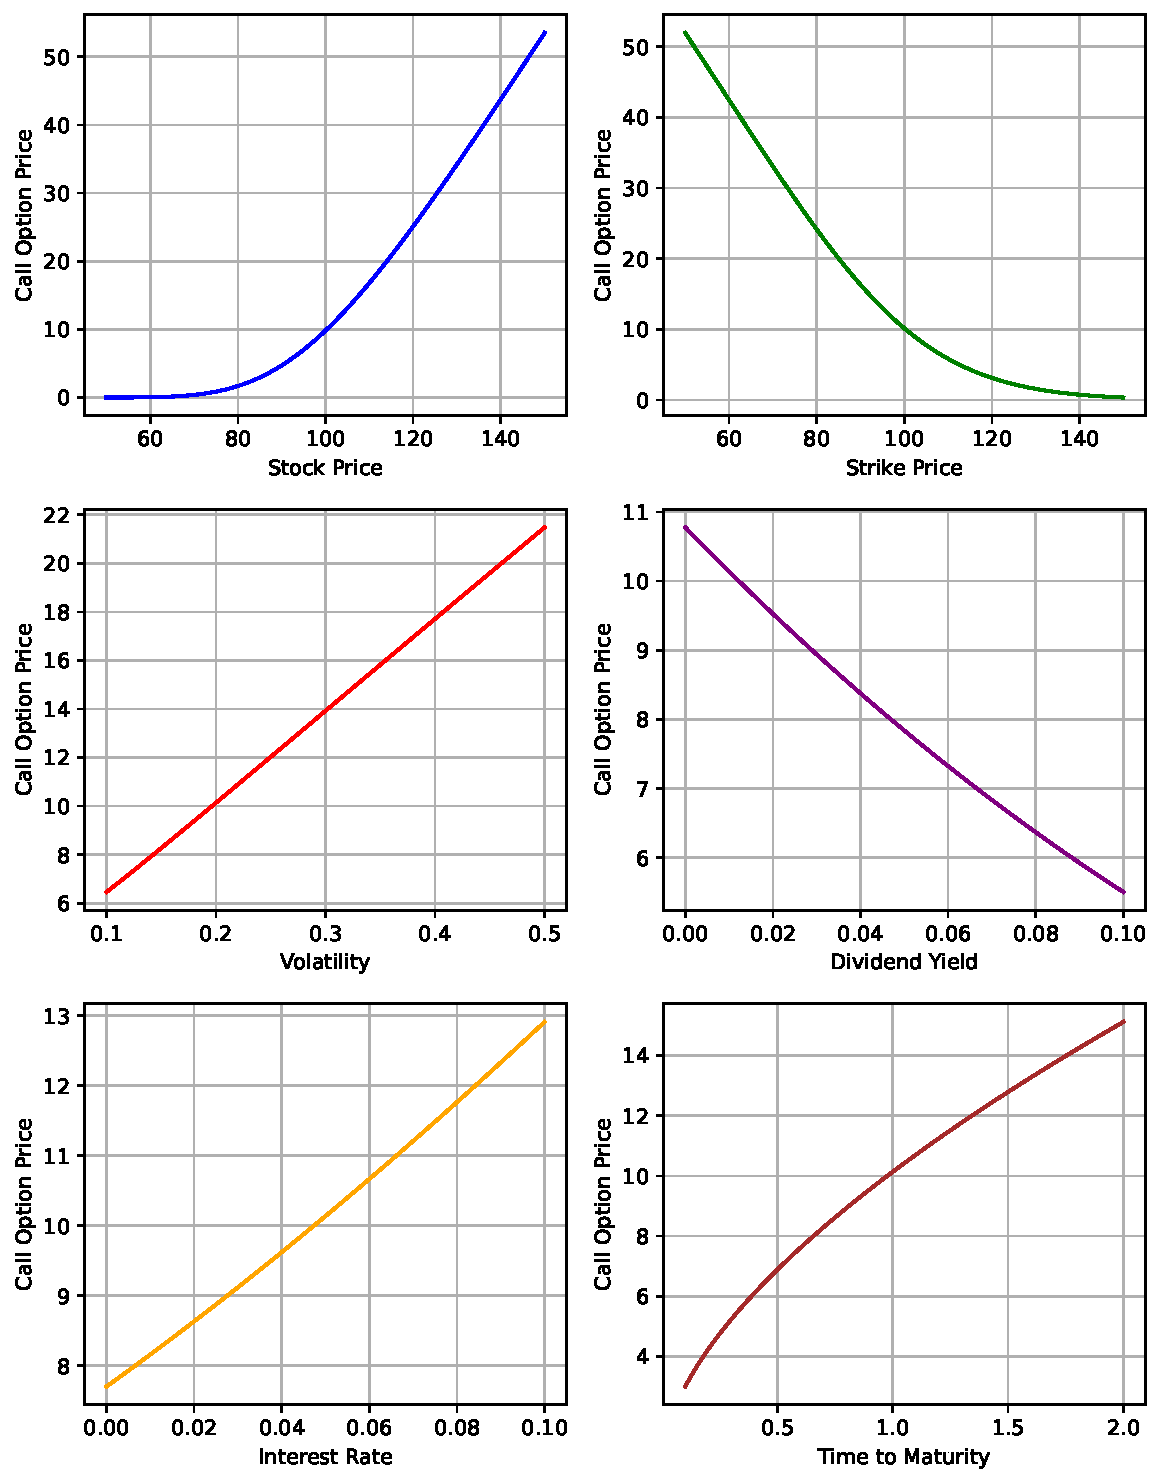
\includegraphics{Chapter4_files/figure-pdf/cell-3-output-1.pdf}

\section{Example: Replicating Portfolios and Simulating Portfolio
Insurance}\label{example-replicating-portfolios-and-simulating-portfolio-insurance}

Another derivation of the Black Scholes formula is provided by Merton.
He asked the question whether by trading the stock and the risk free
asset whether the payoff to a European call option can be replicated.
Let \(\theta_t\) be the number of shares of the stock held at time \(t\)
and \(\alpha_t\) the number of shares of an initial investment of one
dollar in the risk free asset. Then the portfolio is worth
\(\alpha_t R_t + \theta_t S_t\) where \(R_t= e^{rt}\) is the time \(t\)
value of an initial time \(0\) investment of one dollar in the risk free
asset. The portfolio should start with an initial value, should not have
any cash inflows or outflows and have a terminal value equal to a call
payoff so the changes in value are completely dictated by the changes in
the value of the assets. That is, assuming continuous trading,
\[  d W_t = \theta_t d S_t + \alpha_t  d R_t = \theta_t \left(\mu S_t dt + q S_t dt + \sigma S_t d B_t\right)  + \alpha_t r R_t dt\]
with terminal condition
\[ W_T = \alpha_T R_T + \theta_T S_T = (S_T - K)^{+} \] The problem is
to find \(\theta_t\) and \(\alpha_t\) for all times and states. If we
can accomplish this, then by `no-arbitrage' the call price must be the
value of the initial investment. Assume the call price is a function of
the stock price and time: \(C(t,S_t)\). Then by Ito's Lemma
\[ d C(t,S_t) = \left(\frac{\partial C}{\partial t} + \frac{\partial C}{\partial S} (\mu-q) S_t + \frac{1}{2} \frac{\partial^2 C}{\partial S^2} \sigma^2 S_t^2 \right) dt + \frac{\partial C}{\partial S} \sigma S_t dB_t \]
It should be apparent that we want to hold
\(\theta = \frac{\partial C}{\partial S}\), which is the delta of the
call option. By doing so, we match the diffusion term in thw change in
wealth and the change in the call option. Then matching the drift terms
in both expressions
\[ \frac{\partial C}{\partial S} \mu S_t + \alpha_t r R_t = \frac{\partial C}{\partial t} + \frac{\partial C}{\partial S} (\mu-q) S_t + \frac{1}{2} \frac{\partial^2 C}{\partial S^2} \sigma^2 S_t^2\]
which can be solved to give
\[ \alpha_t r R_t=r \left(W_t -\frac{\partial C}{\partial S} S_t\right)  = \frac{\partial C}{\partial t}-\frac{\partial C}{\partial S} q S_t  + \frac{1}{2} \frac{\partial^2 C}{\partial S^2} \sigma^2 S_t^2\]
which gives the equation
\[r W_t = \frac{\partial C}{\partial t} + \frac{\partial C}{\partial S}(r-q) S_t+\frac{1}{2} \frac{\partial^2 C}{\partial S^2} \sigma^2 S_t^2\]
with a boundary condition \(W_T = (S_T-K)^{+}\). However, no-arbitrage
suggests \(W_t = C(t,S_t)\) which gives us the partial differential
equation
\[r C = \frac{\partial C}{\partial t} + \frac{\partial C}{\partial S} (r-q) S+\frac{1}{2} \frac{\partial^2 C}{\partial S^2} \sigma^2 S^2\]
with a boundary condition \(C(T,S_T)= (S_T - K)^{+}\). This is a partial
differential equation and a fairly tedious set of calcuations show the
Black Scholes formula is a solution (in fact it is the only positive
solution). Close observation of the right hand side we see this is the
drift term of Ito expansion for \(C\) if we work in the risk neutral
measure. The right hand side then says in the risk neutral measure, the
call option earns the risk free return.

However, there is nothing special about a call option. The same argument
will apply for any European style option. The only difference is the
boundary condition. This procedure allows us to replicate the payoff of
any European option even for those which might not be traded. This
observation had a profound effect on practice. A particularly popular
example is portfolio insurance.

Recall, that a protective put position buys a put and buys a share and
the payoff at the expiration of the put is given by \(\max(K,S_T)\). The
reason for the name protective put is apparent since the position can
pay off no less than \(K\). The cost of this insurance is the price of
the put. However, if the put is not traded, we can synthetically
replicate this payoff using the prodedure above assuming we can trade
continuously. The basic recipe is to start with inital wealth equal to
that for a protective put position: \(W_0 = P(0,S_0)+S_0\). The delta of
the protective put position can be calcuated to be the delta of the put
plus 1 which is \(N(d_1)\), where \(d_1\) is calculated at each point in
time. However, in practice we cannot trade continuously. A simple
discrete strategy would rebalance at intervals \(\Delta t\). The
strategy calculates \(N(d_1)\) at time 0 and holds
\(P(0,S_0)+S_0 - N(d_1)S_0\) dollars in the risk free asset and
\(N(d_1)\) shares of the asset. Thereafter these holdings are adjusted.
The change in portfolio value over the interval \(\Delta t\) is
\[\Delta W= W_{i \Delta t}- W_{(i-1)\Delta t} \] \[ 
= (P((i-1)\Delta t,S_{(i-1)\Delta t})+S_{(i-1)\Delta t} - N(d_1-)S_{(i-1)\Delta t})(R_{i\Delta t}-R_{(i-1)\Delta t}) + N(d1-)(S_{i\Delta t}-S_{(i-1)\Delta t}) 
\] where \(N(d1-)\) is the delta chosen at time \((i-1)\Delta t\). The
question is if the Black Scoles model is correct, how accurate can a
discrete rebalancing scheme be? This is simulated in the following code:

\begin{Shaded}
\begin{Highlighting}[]
\ImportTok{import}\NormalTok{ numpy }\ImportTok{as}\NormalTok{ np}
\CommentTok{\# from bsfunctions import *}
\ImportTok{import}\NormalTok{ matplotlib.pyplot }\ImportTok{as}\NormalTok{ plt}
\ImportTok{import}\NormalTok{ time}
\ImportTok{from}\NormalTok{ math }\ImportTok{import} \BuiltInTok{pow}\NormalTok{, exp, sqrt}
\ImportTok{from}\NormalTok{ scipy }\ImportTok{import}\NormalTok{ stats}
\CommentTok{\# incs = np.genfromtxt(\textquotesingle{}incs.csv\textquotesingle{},delimiter=",",skip\_header=1)}
\KeywordTok{def}\NormalTok{ blackscholes(S0, K, r, q, sig, T, call }\OperatorTok{=} \VariableTok{True}\NormalTok{):}
    \CommentTok{\textquotesingle{}\textquotesingle{}\textquotesingle{}Calculate option price using B{-}S formula.}

\CommentTok{    Args:}
\CommentTok{        S0 (num): initial price of underlying asset.}
\CommentTok{        K (num): strick price.}
\CommentTok{        r (num): risk free rate.}
\CommentTok{        q (num): dividend yield}
\CommentTok{        sig (num): Black{-}Scholes volatility.}
\CommentTok{        T (num): maturity.}
\CommentTok{        call (bool): True returns call price, False returns put price.}

\CommentTok{    Returns:}
\CommentTok{        num}
\CommentTok{    \textquotesingle{}\textquotesingle{}\textquotesingle{}}
\NormalTok{    d1 }\OperatorTok{=}\NormalTok{ (np.log(S0}\OperatorTok{/}\NormalTok{K) }\OperatorTok{+}\NormalTok{ (r }\OperatorTok{{-}}\NormalTok{q }\OperatorTok{+}\NormalTok{ sig}\OperatorTok{**}\DecValTok{2}\OperatorTok{/}\DecValTok{2}\NormalTok{) }\OperatorTok{*}\NormalTok{ T)}\OperatorTok{/}\NormalTok{(sig}\OperatorTok{*}\NormalTok{np.sqrt(T))}
\NormalTok{    d2 }\OperatorTok{=}\NormalTok{ d1 }\OperatorTok{{-}}\NormalTok{ sig}\OperatorTok{*}\NormalTok{np.sqrt(T)}
\CommentTok{\#     norm = sp.stats.norm}
\NormalTok{    norm }\OperatorTok{=}\NormalTok{ stats.norm}
    \ControlFlowTok{if}\NormalTok{ call:}
        \ControlFlowTok{return}\NormalTok{ np.exp(}\OperatorTok{{-}}\NormalTok{q}\OperatorTok{*}\NormalTok{T)}\OperatorTok{*}\NormalTok{S0 }\OperatorTok{*}\NormalTok{ norm.cdf(d1,}\DecValTok{0}\NormalTok{,}\DecValTok{1}\NormalTok{) }\OperatorTok{{-}}\NormalTok{ K }\OperatorTok{*}\NormalTok{ np.exp(}\OperatorTok{{-}}\NormalTok{r }\OperatorTok{*}\NormalTok{ T) }\OperatorTok{*}\NormalTok{ norm.cdf(d2,}\DecValTok{0}\NormalTok{, }\DecValTok{1}\NormalTok{)}
    \ControlFlowTok{else}\NormalTok{:}
        \ControlFlowTok{return}\NormalTok{ np.exp(}\OperatorTok{{-}}\NormalTok{q}\OperatorTok{*}\NormalTok{T)}\OperatorTok{*}\NormalTok{S0 }\OperatorTok{*} \OperatorTok{{-}}\NormalTok{norm.cdf(}\OperatorTok{{-}}\NormalTok{d1,}\DecValTok{0}\NormalTok{,}\DecValTok{1}\NormalTok{) }\OperatorTok{+}\NormalTok{ K }\OperatorTok{*}\NormalTok{ np.exp(}\OperatorTok{{-}}\NormalTok{r }\OperatorTok{*}\NormalTok{ T) }\OperatorTok{*}\NormalTok{ norm.cdf(}\OperatorTok{{-}}\NormalTok{d2,}\DecValTok{0}\NormalTok{, }\DecValTok{1}\NormalTok{)}

\KeywordTok{def}\NormalTok{ blackscholes\_delta(S0, K, r, q, sig, T, call }\OperatorTok{=} \VariableTok{True}\NormalTok{):}
    \CommentTok{\textquotesingle{}\textquotesingle{}\textquotesingle{}Calculate option price using B{-}S formula.}

\CommentTok{    Args:}
\CommentTok{        S0 (num): initial price of underlying asset.}
\CommentTok{        K (num): strick price.}
\CommentTok{        r (num): risk free rate.}
\CommentTok{        q (num): dividend yield}
\CommentTok{        sig (num): Black{-}Scholes volatility.}
\CommentTok{        T (num): maturity.}
\CommentTok{        call (bool): True returns call price, False returns put price.}

\CommentTok{    Returns:}
\CommentTok{        num}
\CommentTok{    \textquotesingle{}\textquotesingle{}\textquotesingle{}}
\NormalTok{    d1 }\OperatorTok{=}\NormalTok{ (np.log(S0}\OperatorTok{/}\NormalTok{K) }\OperatorTok{+}\NormalTok{ (r }\OperatorTok{{-}}\NormalTok{q }\OperatorTok{+}\NormalTok{ sig}\OperatorTok{**}\DecValTok{2}\OperatorTok{/}\DecValTok{2}\NormalTok{) }\OperatorTok{*}\NormalTok{ T)}\OperatorTok{/}\NormalTok{(sig}\OperatorTok{*}\NormalTok{np.sqrt(T))}
\NormalTok{    d2 }\OperatorTok{=}\NormalTok{ d1 }\OperatorTok{{-}}\NormalTok{ sig}\OperatorTok{*}\NormalTok{np.sqrt(T)}
\CommentTok{\#     norm = sp.stats.norm}
\NormalTok{    norm }\OperatorTok{=}\NormalTok{ stats.norm}
    \ControlFlowTok{if} \BuiltInTok{type}\NormalTok{(call) }\OperatorTok{==} \BuiltInTok{bool}\NormalTok{:}
        \ControlFlowTok{if}\NormalTok{ call:}
            \ControlFlowTok{return}\NormalTok{ np.exp(}\OperatorTok{{-}}\NormalTok{q}\OperatorTok{*}\NormalTok{T)}\OperatorTok{*}\NormalTok{norm.cdf(d1,}\DecValTok{0}\NormalTok{,}\DecValTok{1}\NormalTok{)}
        \ControlFlowTok{else}\NormalTok{:}
            \ControlFlowTok{return}\NormalTok{ np.exp(}\OperatorTok{{-}}\NormalTok{q}\OperatorTok{*}\NormalTok{T)}\OperatorTok{*}\NormalTok{norm.cdf(}\OperatorTok{{-}}\NormalTok{d1,}\DecValTok{0}\NormalTok{,}\DecValTok{1}\NormalTok{)}
    \ControlFlowTok{else}\NormalTok{:}
        \BuiltInTok{print}\NormalTok{(}\StringTok{"Not a valid value for call"}\NormalTok{)}

\CommentTok{\# parameters}
\CommentTok{\# number of paths}
\CommentTok{\# n = incs.shape[1]}
\NormalTok{n }\OperatorTok{=} \DecValTok{100000}
\CommentTok{\# number of divisions}
\CommentTok{\# m = incs.shape[0]}
\NormalTok{m }\OperatorTok{=} \DecValTok{100}
\CommentTok{\# interest rate}
\NormalTok{r }\OperatorTok{=} \FloatTok{.1}
\CommentTok{\# dividend yield}
\NormalTok{q}\OperatorTok{=}\FloatTok{0.0}
\CommentTok{\# true drift}
\NormalTok{mu }\OperatorTok{=} \FloatTok{.15}
\CommentTok{\# volatility}
\NormalTok{sig }\OperatorTok{=} \FloatTok{.2}
\CommentTok{\# Initial Stock Price}
\NormalTok{S0 }\OperatorTok{=} \DecValTok{42}
\CommentTok{\# Strike Price}
\NormalTok{K }\OperatorTok{=} \DecValTok{42}
\CommentTok{\# Maturity}
\NormalTok{T }\OperatorTok{=} \FloatTok{0.5}


\CommentTok{\# seed for random generator}
\NormalTok{seed}\OperatorTok{=} \DecValTok{1234}
\CommentTok{\# define a random generator}
\NormalTok{rg }\OperatorTok{=}\NormalTok{ np.random.RandomState(seed)}
\CommentTok{\# initialize}


\CommentTok{\# generate normal random vairables}
\NormalTok{dt}\OperatorTok{=}\NormalTok{ T}\OperatorTok{/}\NormalTok{m}
\NormalTok{vol}\OperatorTok{=}\NormalTok{sig}\OperatorTok{*}\NormalTok{np.sqrt(dt)}
\NormalTok{incs }\OperatorTok{=}\NormalTok{ rg.normal(}\DecValTok{0}\NormalTok{,vol,[m,n])}


\NormalTok{tline }\OperatorTok{=}\NormalTok{ np.linspace(}\DecValTok{0}\NormalTok{,T,m}\OperatorTok{+}\DecValTok{1}\NormalTok{)}


\NormalTok{St }\OperatorTok{=}\NormalTok{ np.zeros((m}\OperatorTok{+}\DecValTok{1}\NormalTok{,n))}
\CommentTok{\#St1 = np.zeros((m+1,n))}

\NormalTok{V\_vec }\OperatorTok{=}\NormalTok{ np.zeros((m}\OperatorTok{+}\DecValTok{1}\NormalTok{,n))}

\NormalTok{delta }\OperatorTok{=}\NormalTok{ np.zeros((m,n))}

\NormalTok{put}\OperatorTok{=}\NormalTok{ blackscholes(S0,K,r, q, sig,T,call}\OperatorTok{=}\VariableTok{False}\NormalTok{)}

\NormalTok{incs\_cumsum }\OperatorTok{=}\NormalTok{  np.concatenate((np.zeros((}\DecValTok{1}\NormalTok{,n)),incs),axis}\OperatorTok{=}\DecValTok{0}\NormalTok{).cumsum(axis}\OperatorTok{=}\DecValTok{0}\NormalTok{)}
\NormalTok{V\_vec }\OperatorTok{=}\NormalTok{ np.zeros((m}\OperatorTok{+}\DecValTok{1}\NormalTok{,n))}
\NormalTok{t\_mat }\OperatorTok{=}\NormalTok{  np.repeat(tline.reshape((m}\OperatorTok{+}\DecValTok{1}\NormalTok{,}\DecValTok{1}\NormalTok{)), n, axis}\OperatorTok{=}\DecValTok{1}\NormalTok{)}
\NormalTok{drift\_cumsum }\OperatorTok{=}\NormalTok{ (mu }\OperatorTok{{-}}\NormalTok{q }\OperatorTok{{-}}\FloatTok{0.5}\OperatorTok{*}\NormalTok{sig}\OperatorTok{**}\DecValTok{2}\NormalTok{) }\OperatorTok{*}\NormalTok{ t\_mat}

\NormalTok{St }\OperatorTok{=}\NormalTok{ S0 }\OperatorTok{*}\NormalTok{ np.exp(incs\_cumsum }\OperatorTok{+}\NormalTok{ drift\_cumsum)}

\NormalTok{delta }\OperatorTok{=}\NormalTok{ blackscholes\_delta(St[:}\OperatorTok{{-}}\DecValTok{1}\NormalTok{,:],K,r, q, sig,T}\OperatorTok{{-}}\NormalTok{t\_mat[:}\OperatorTok{{-}}\DecValTok{1}\NormalTok{,:])}

\NormalTok{V\_vec[}\DecValTok{0}\NormalTok{,:] }\OperatorTok{=}\NormalTok{ S0 }\OperatorTok{+}\NormalTok{ put}

\ControlFlowTok{for}\NormalTok{ i }\KeywordTok{in} \BuiltInTok{range}\NormalTok{(}\DecValTok{1}\NormalTok{,m}\OperatorTok{+}\DecValTok{1}\NormalTok{):}
\NormalTok{    V\_vec[i,:] }\OperatorTok{=}\NormalTok{ V\_vec[i}\OperatorTok{{-}}\DecValTok{1}\NormalTok{,:] }\OperatorTok{+}\NormalTok{ (np.exp(r}\OperatorTok{*}\NormalTok{dt)}\OperatorTok{{-}}\DecValTok{1}\NormalTok{) }\OperatorTok{*}\NormalTok{ (V\_vec[i}\OperatorTok{{-}}\DecValTok{1}\NormalTok{,:] }\OperatorTok{{-}}\NormalTok{ delta[i}\OperatorTok{{-}}\DecValTok{1}\NormalTok{,:] }\OperatorTok{*}\NormalTok{ St[i}\OperatorTok{{-}}\DecValTok{1}\NormalTok{,:])}\OperatorTok{+}\NormalTok{ delta[i}\OperatorTok{{-}}\DecValTok{1}\NormalTok{,:] }\OperatorTok{*}\NormalTok{ (St[i,:]}\OperatorTok{{-}}\NormalTok{St[i}\OperatorTok{{-}}\DecValTok{1}\NormalTok{,:])}

\CommentTok{\# Uses actual simulated changes in riskfree and stock price not the dt and dB approximations }
\CommentTok{\# plot ST versus VT}
\NormalTok{plt.scatter(St[m,:],V\_vec[m,:])}
\NormalTok{plt.xlabel(}\StringTok{\textquotesingle{}Stock Price at Maturity\textquotesingle{}}\NormalTok{)}
\NormalTok{plt.ylabel(}\StringTok{\textquotesingle{}Value of Portfolio Insurance\textquotesingle{}}\NormalTok{)}
\NormalTok{plt.show()}
\end{Highlighting}
\end{Shaded}

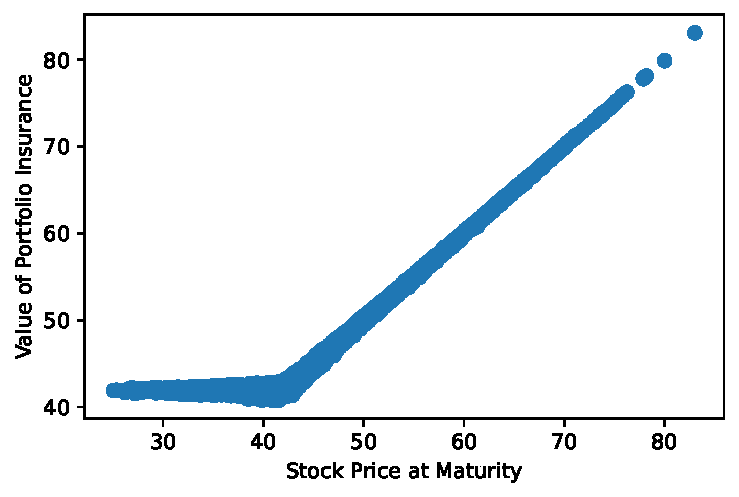
\includegraphics{Chapter4_files/figure-pdf/cell-4-output-1.pdf}

With \(m=100\) rebalancing dates over \(T=0.5\) for the parameters
chosen the repliacting strategy does a pretty good job. The hedging
errors occur when the stock price is close to the strike price. This is
not surprising since the delta changes (measured by the gamma) fastest
around this point. A gamma hedge would potentially improve the
performance.

The portfolio insurance rebalancing scheme involves sell stock and
buying bonds when the stock price goes down and buying stocks and
selling bonds when the stock price goes up. This can be destabilizing
and was identified as a contributor to the 1987 stock market crash.

\subsection{Discretely-Rebalanced Delta
Hedges}\label{discretely-rebalanced-delta-hedges}

To compute the real-world distribution of gains and losses from a
discretely-rebalanced delta hedge, we input the expected rate of return
\(\mu\). We consider adjusting the hedge at dates
\(0=t_0<t_1<\cdots<t_N=T\), with \(t_i-t_{i-1}=\Delta t = T/N\) for each
\(i\). The changes in the natural logarithm of the stock price between
successive dates \(t_{i-1}\) and \(t_i\) are simulated as
\[\Delta \log S = \left(\mu-q-\frac{1}{2}\sigma^2\right)\,\Delta t + \sigma\,\Delta B\; ,\]
where \(\Delta B\) is normally distributed with mean zero and variance
\(\Delta t\). The random variables \(\Delta B\) are simulated as
standard normals multiplied by \(\sqrt{\Delta t}\). We begin with the
portfolio that is short a call, long \(\delta\) shares of the
underlying, and short \(\delta S-C\) in cash. After the stock price
changes, say from \(S\) to \(S'\), we compute the new delta \(\delta'\).
The cash flow from adjusting the hedge is \((\delta-\delta')S'\).
Accumulation (or payment) of interest on the cash position is captured
by the factor \(e^{r\Delta t}\). Continuous payment of dividends is
modelled similarly: the dividends earned during the period \(\Delta t\)
is taken to be \(\delta S\left(e^{q\Delta t}-1\right)\). The cash
position is adjusted due to interest, dividends, and the cash flow from
adjusting the hedge. At date \(T\), the value of the portfolio is the
cash position less the intrinsic value of the option.

To describe the distribution of gains and losses, we compute percentiles
of the distribution. You should see that the hedge becomes more nearly
perfect as the number of periods \(N\) is increased. Note that this is
true regardless of the \(\mu\) that is input, which reaffirms the point
that option values and hedges do not depend on the expected rate of
return of the underlying. The percentile is calculated with the Excel
\verb!Percentile! function.\footnote{If numsims = 11 and pct =0.1, the
  percentile function returns the second lowest element in the series.
  The logic is that 10\% of the numbers, excluding the number returned,
  are below the number returned---i.e., 1 out of the other 10 are
  below---and 90\% of the others are above. In particular, if pct = 0.5,
  the percentile function returns the median. When necessary, the
  function interpolates; for example, if numsims = 10 and pct=0.1, then
  the number returned is an interpolation between the lowest and second
  lowest numbers.}

\begin{Shaded}
\begin{Highlighting}[]
\ImportTok{import}\NormalTok{ numpy }\ImportTok{as}\NormalTok{ np}
\ImportTok{from}\NormalTok{ scipy.stats }\ImportTok{import}\NormalTok{ norm}
\ImportTok{import}\NormalTok{ scipy.optimize }\ImportTok{as}\NormalTok{ optimize}

\KeywordTok{def}\NormalTok{ simulated\_delta\_hedge\_profit(S0, K, r, sigma, q, T, mu, M, N, pct):}
    \CommentTok{"""}
\CommentTok{    Inputs:}
\CommentTok{    S0 = initial stock price}
\CommentTok{    K = strike price}
\CommentTok{    r = risk{-}free rate}
\CommentTok{    sigma = volatility}
\CommentTok{    q = dividend yield}
\CommentTok{    T = time to maturity}
\CommentTok{    mu = expected rate of return}
\CommentTok{    N = number of time periods}
\CommentTok{    M = number of simulations}
\CommentTok{    pct = percentile to be returned}
\CommentTok{    """}
\NormalTok{    dt }\OperatorTok{=}\NormalTok{ T }\OperatorTok{/}\NormalTok{ N}
\NormalTok{    SigSqrdt }\OperatorTok{=}\NormalTok{ sigma }\OperatorTok{*}\NormalTok{ np.sqrt(dt)}
\NormalTok{    drift }\OperatorTok{=}\NormalTok{ (mu }\OperatorTok{{-}}\NormalTok{ q }\OperatorTok{{-}} \FloatTok{0.5} \OperatorTok{*}\NormalTok{ sigma }\OperatorTok{**} \DecValTok{2}\NormalTok{) }\OperatorTok{*}\NormalTok{ dt}
\NormalTok{    Comp }\OperatorTok{=}\NormalTok{ np.exp(r }\OperatorTok{*}\NormalTok{ dt)}
\NormalTok{    Div }\OperatorTok{=}\NormalTok{ np.exp(q }\OperatorTok{*}\NormalTok{ dt) }\OperatorTok{{-}} \DecValTok{1}
\NormalTok{    LogS0 }\OperatorTok{=}\NormalTok{ np.log(S0)}
\NormalTok{    Call0 }\OperatorTok{=}\NormalTok{ black\_scholes\_call(S0, K, r, sigma, q, T)}
\NormalTok{    Delta0 }\OperatorTok{=}\NormalTok{ black\_scholes\_call\_delta(S0, K, r, sigma, q, T)}
\NormalTok{    Cash0 }\OperatorTok{=}\NormalTok{ Call0 }\OperatorTok{{-}}\NormalTok{ Delta0 }\OperatorTok{*}\NormalTok{ S0}
\NormalTok{    Profit }\OperatorTok{=}\NormalTok{ np.zeros(M)}

    \ControlFlowTok{for}\NormalTok{ i }\KeywordTok{in} \BuiltInTok{range}\NormalTok{(M):}
\NormalTok{        LogS }\OperatorTok{=}\NormalTok{ LogS0}
\NormalTok{        Cash }\OperatorTok{=}\NormalTok{ Cash0}
\NormalTok{        S }\OperatorTok{=}\NormalTok{ S0}
\NormalTok{        Delta }\OperatorTok{=}\NormalTok{ Delta0}

        \ControlFlowTok{for}\NormalTok{ j }\KeywordTok{in} \BuiltInTok{range}\NormalTok{(}\DecValTok{1}\NormalTok{, N):}
\NormalTok{            LogS }\OperatorTok{+=}\NormalTok{ drift }\OperatorTok{+}\NormalTok{ SigSqrdt }\OperatorTok{*}\NormalTok{ np.random.randn()}
\NormalTok{            NewS }\OperatorTok{=}\NormalTok{ np.exp(LogS)}
\NormalTok{            NewDelta }\OperatorTok{=}\NormalTok{ black\_scholes\_call\_delta(NewS, K, r, sigma, q, T }\OperatorTok{{-}}\NormalTok{ j }\OperatorTok{*}\NormalTok{ dt)}
\NormalTok{            Cash }\OperatorTok{=}\NormalTok{ Comp }\OperatorTok{*}\NormalTok{ Cash }\OperatorTok{+}\NormalTok{ Delta }\OperatorTok{*}\NormalTok{ S }\OperatorTok{*}\NormalTok{ Div }\OperatorTok{{-}}\NormalTok{ (NewDelta }\OperatorTok{{-}}\NormalTok{ Delta) }\OperatorTok{*}\NormalTok{ NewS}
\NormalTok{            S }\OperatorTok{=}\NormalTok{ NewS}
\NormalTok{            Delta }\OperatorTok{=}\NormalTok{ NewDelta}

\NormalTok{        LogS }\OperatorTok{+=}\NormalTok{ drift }\OperatorTok{+}\NormalTok{ SigSqrdt }\OperatorTok{*}\NormalTok{ np.random.randn()}
\NormalTok{        NewS }\OperatorTok{=}\NormalTok{ np.exp(LogS)}
\NormalTok{        HedgeValue }\OperatorTok{=}\NormalTok{ Comp }\OperatorTok{*}\NormalTok{ Cash }\OperatorTok{+}\NormalTok{ Delta }\OperatorTok{*}\NormalTok{ S }\OperatorTok{*}\NormalTok{ Div }\OperatorTok{+}\NormalTok{ Delta }\OperatorTok{*}\NormalTok{ NewS}
\NormalTok{        Profit[i] }\OperatorTok{=}\NormalTok{ HedgeValue }\OperatorTok{{-}} \BuiltInTok{max}\NormalTok{(NewS }\OperatorTok{{-}}\NormalTok{ K, }\DecValTok{0}\NormalTok{)}

    \ControlFlowTok{return}\NormalTok{ np.percentile(Profit, pct }\OperatorTok{*} \DecValTok{100}\NormalTok{)}

\CommentTok{\# Example usage (you can replace these with input values)}
\NormalTok{S }\OperatorTok{=} \DecValTok{100}  \CommentTok{\# Initial stock price}
\NormalTok{K }\OperatorTok{=} \DecValTok{100}  \CommentTok{\# Strike price}
\NormalTok{r }\OperatorTok{=} \FloatTok{0.05}  \CommentTok{\# Risk{-}free rate}
\NormalTok{sigma }\OperatorTok{=} \FloatTok{0.2}  \CommentTok{\# Volatility}
\NormalTok{q }\OperatorTok{=} \FloatTok{0.02}  \CommentTok{\# Dividend yield}
\NormalTok{T }\OperatorTok{=} \DecValTok{1}  \CommentTok{\# Time to maturity in years}
\NormalTok{CallPrice }\OperatorTok{=} \DecValTok{10}  \CommentTok{\# Call price for implied volatility calculation}

\CommentTok{\# Simulate delta hedging profit}
\NormalTok{S0 }\OperatorTok{=} \DecValTok{100}  \CommentTok{\# Initial stock price}
\NormalTok{mu }\OperatorTok{=} \FloatTok{0.1}  \CommentTok{\# Expected rate of return}
\NormalTok{M }\OperatorTok{=} \DecValTok{1000}  \CommentTok{\# Number of simulations}
\NormalTok{N }\OperatorTok{=} \DecValTok{252}  \CommentTok{\# Number of time periods}
\NormalTok{pct }\OperatorTok{=} \FloatTok{0.95}  \CommentTok{\# Percentile to be returned}

\NormalTok{delta\_hedge\_profit }\OperatorTok{=}\NormalTok{ simulated\_delta\_hedge\_profit(S0, K, r, sigma, q, T, mu, M, N, pct)}
\BuiltInTok{print}\NormalTok{(}\SpecialStringTok{f"Delta Hedge Profit (95th percentile): }\SpecialCharTok{\{}\NormalTok{delta\_hedge\_profit}\SpecialCharTok{\}}\SpecialStringTok{"}\NormalTok{)}
\end{Highlighting}
\end{Shaded}

\begin{verbatim}
Delta Hedge Profit (95th percentile): 0.6283250482023715
\end{verbatim}

\section{Exercises}\label{exercises-2}

\begin{exercise}[]\protect\hypertarget{exr-problem4.1}{}\label{exr-problem4.1}

Create a Python code which inputs \(K\), \(r\), \(\sigma\), \(q\) and
\(T\). Compute the delta of a call option for stock prices \(S = .01K\),
\(.02K\), \ldots, \(1.99K\), \(2K\) (i.e., \(S = iK/100\) for
\(i=1, \ldots 200\)) and plot the delta against the stock price.

\end{exercise}

\begin{exercise}[]\protect\hypertarget{exr-nolabel}{}\label{exr-nolabel}

The delta of a digital option that pays \$1 when \(S(T)>K\) is
\[\frac{\mathrm{e}^{-rT}\mathrm{n}d(d_2)}{\sigma S\sqrt{T}}\; .\] Repeat
the previous problem for the delta of this digital. Given that in
reality it is costly to trade (due to commissions, the bid-ask spread
and possible adverse price impacts for large trades), do you see any
problems with delta hedging a short digital near maturity if it is close
to being at the money?

\end{exercise}

\begin{exercise}[]\protect\hypertarget{exr-nolabel}{}\label{exr-nolabel}

Modify the Python code for replicating portfolio insurance to simulate a
discrete replication of a digital option using the delta in the previous
problem. Run the code for \(10,20,100,1000\) rebalancing dates. When
does the strategy do a good job and when does it fail?

\end{exercise}

\begin{exercise}[]\protect\hypertarget{exr-nolabel}{}\label{exr-nolabel}

Repeat Exercise~\ref{exr-problem4.1} for the gamma of a call option.

\end{exercise}

\begin{exercise}[]\protect\hypertarget{exr-nolabel}{}\label{exr-nolabel}

Consider delta and gamma hedging a short call option, using the
underlying and a put with the same strike and maturity as the call.
Calculate the position in the underlying and the put that you should
take, using the analysis in Section~\ref{sec-s_gammahedging}. Will you
ever need to adjust this hedge? Relate your result to put-call parity.

\end{exercise}

\begin{exercise}[]\protect\hypertarget{exr-nolabel}{}\label{exr-nolabel}

The delta of a share digital that pays one share when \(S(T)>K\) is
\[\mathrm{e}^{-qT}\mathrm{N}(d_1) + \frac{\mathrm{e}^{-qT}\mathrm{n}d(d_1)}{\sigma \sqrt{T}}\; .\]
Repeat Exercise~\ref{exr-problem4.1} for the delta of this share
digital.

\end{exercise}

\begin{exercise}[]\protect\hypertarget{exr-nolabel}{}\label{exr-nolabel}

Compute the value of an at-the-money call option (\(S=K\)) using the
Python code for volatilities \(\sigma = .01, .02, \ldots, 1.0\). Plot
the call value against the volatility.

\end{exercise}

\begin{exercise}[]\protect\hypertarget{exr-nolabel}{}\label{exr-nolabel}

Repeat the previous problem for \(S=1.2K\) (an example of an
in-the-money call option).

\end{exercise}

\begin{exercise}[]\protect\hypertarget{exr-nolabel}{}\label{exr-nolabel}

The file CBOEQuotes.txt (available at \verb!www.kerryback.net!) contains
price data for call options on the S\&P 500 index. The options expired
in February, 2003, and the prices were obtained on January 22, 2003. The
first column lists various exercise prices. The second column gives the
bid price and the third column the ask price. Import this data into an
Excel worksheet and compute and plot the implied volatility against the
exercise price using this data. Use the ask price as the market price
for the option. The options have 30 days to maturity (so \(T=30/365\)).
At the time the quotes were downloaded, the S\&P 500 was at 884.25.
According to the CBOE, the dividend yield on the S\&P 500 was 1.76\%.
Use 1.25\% for the risk-free interest rate.

\end{exercise}

\begin{exercise}[]\protect\hypertarget{exr-nolabel}{}\label{exr-nolabel}

Attempt to repeat the previous problem using the bid price as the market
price of the option. If this doesn't work, what is wrong? Does this
indicate there is an arbitrage opportunity?

\end{exercise}

::: Suppose an investor invests in a portfolio with price \(S\) and
constant dividend yield \(q\). Assume the investor is charged a constant
expense ratio \(\alpha\) (which acts as a negative dividend) and at date
\(T\) receives either his portfolio value or his initial investment,
whichever is higher. This is similar to a popular type of variable
annuity. Letting \(D\) denote the number of dollars invested in the
contract, the contract pays
\begin{equation}\phantomsection\label{eq-bsp1}{
\max\left(D,\frac{D\mathrm{e}^{(q-\alpha)T}S(T)}{S(0)}\right)
}\end{equation} at date \(T\).\\
We can rearrange the expression Equation~\ref{eq-bsp1} as

\[
\max\left(D,\frac{D\mathrm{e}^{(q-\alpha)T}S(T)}{S(0)}\right) = D + \max\left(0, \frac{D\mathrm{e}^{(q-\alpha)T}S(T)}{S(0)}-D\right)
\] \begin{equation}\phantomsection\label{eq-bsp2}{
= D + \mathrm{e}^{-\alpha T}D\max\left(0,\frac{\mathrm{e}^{qT}S(T)}{S(0)}-\mathrm{e}^{\alpha T}\right)\;.
}\end{equation}

Thus, the contract payoff is equivalent to the amount invested plus a
certain number of call options written on the gross holding period
return \(\mathrm{e}^{qT}S(T)/S(0)\). Note that
\(Z(t) = \mathrm{e}^{qt}S(t)/S(0)\) is the date--\(t\) value of the
portfolio that starts with \(1/S(0)\) units of the asset (i.e., with a
\$1 investment) and reinvests dividends. Thus, the call options are call
options on a non-dividend paying portfolio with the same volatility as
\(S\) and initial price of \$1. This implies that the date--0 value of
the contract to the investor is \(\mathrm{e}^{-rT}D\) plus

\(e^{-\alpha*T}*D*\)\texttt{Black\_Scholes\_Call}\((1,e^{-\alpha*T},r,sigma,q,T)\)

\begin{enumerate}
\def\labelenumi{\arabic{enumi}.}
\tightlist
\item
  Create a Python function to compute the fair expense ratio; i.e., find
  \(\alpha\) such that the date--0 value of the contract is equal to
  \(D\). Hint: Modify the
\end{enumerate}

\texttt{Black\_Scholes\_Call\_Implied\_Vol}

function. You can use \(\alpha=0\) as a lower bound. Because the value
of the contract is decreasing as \(\alpha\) increases, you can find an
upper bound by iterating until the value of the contract is less than
\(D\). 2. How does the fair expense ratio vary with the maturity \(T\)?
Why?

::: ::: \{\#exr-nolabel\} Modify the function
\verb!Simulated_Delta_Hedge_Profit! to compute percentiles of gains and
losses for an investor who writes a call option and constructs a delta
and gamma hedge using the underlying asset and another call option.
Include the exercise price of the call option used to hedge as an input,
and assume it has the same time to maturity as the option that is
written. Hint: In each period \verb!j = 1 to N-1!, the updated cash
position can be calculated as

\begin{verbatim}
Cash = exp(r*dt)*Cash + a*S*(exp(q*dt)-1) - (Newa-a)*NewS _
     - (Newb-b)*PriceHedge ,
\end{verbatim}

where \verb!a! denotes the number of shares of the stock held, \verb!b!
denotes the number of units held of the option that is used for hedging,
and \verb!PriceHedge! denotes the price of the option used for hedging
(computed from the Black-Scholes formula each period). This expression
embodies the interest earned (paid) on the cash position, the dividends
received on the shares of stock and the cash inflows (outflows) from
adjusting the hedge. At the final date \verb!N!, the value of the hedge
is

\begin{verbatim}
exp(r*dt)*Cash + a*S*(exp(q*dt)-1) + a*NewS _
     + b*Application.Max(NewS-KHedge,0) ,
 \end{verbatim}

and the value of the overall portfolio is the value of the hedge less

\begin{verbatim}
Application.Max(NewS-KWritten,0) ,
 \end{verbatim}

where \verb!KHedge! denotes the strike price of the option used to hedge
and \verb!KWritten! denotes the strike of the option that was written.
:::

\bookmarksetup{startatroot}

\chapter{Estimating and Modeling
Volatility}\label{sec-c_stochasticvolatility}

Thus far, we have assumed that the volatility of the underlying asset is
constant or varying in a non-random way during the lifetime of the
derivative. In this chapter we will look at models that relax this
assumption and allow the volatility to change randomly. This is very
important, because there is plenty of evidence that volatilities do
change over time in a random way.

In the first three sections, we will consider the problem of estimating
the volatility. The discussion of estimation methods leads naturally
into the discussion of modeling a changing volatility.

\section{Statistics Review}\label{sec-s_statistics}

We begin with a brief review of basic statistics. Given a random sample
\(\{x_1,\ldots,x_N\}\) of size \(N\) from a population with mean \(\mu\)
and variance \(\sigma^2\), the best estimate of \(\mu\) is of course the
sample mean \[\bar{x} = \frac{1}{N}\sum_{i=1}^{N}x_i\; .\] The variance
is the expected value of \((x-\mu)^2\), so an obvious estimate of the
variance is the sample average of \((x_i-\mu)^2\), replacing \(\mu\)
with its estimate \(\bar{x}\). This would be
\[\frac{1}{N}\sum_{i=1}^{N} (x_i-\bar{x})^2\] However, because
\(\bar{x}\) is computed from the \(x_i\), the \(x_i\) will deviate less
on average from \(\bar{x}\) than they do from the true mean \(\mu\).
Hence the estimate proposed above will on average be less than
\(\sigma^2\). To eliminate this bias, it suffices just to scale the
estimate up by a factor of \(N/(N-1)\). This leads to the estimate
\[s^2=\frac{1}{N-1}\sum_{i=1}^{N} (x_i-\bar{x})^2\; ,\] and the best
estimate of \(\sigma\) is the square root
\[s=\sqrt{\frac{1}{N-1}\sum_{i=1}^{N} (x_i-\bar{x})^2}\; .\] To
calculate \(s^2\), notice that \begin{align*}
\sum_{i=1}^{N} (x_i-\bar{x})^2 &= \sum_{i=1}^{N} (x_i^2-2x_i\bar{x}+\bar{x}^2)\\
&=\sum_{i=1}^{N} x_i^2 -2\bar{x}\sum_{i=1}^{N} x_i + \sum_{i=1}^N \bar{x}^2\\
&=\sum_{i=1}^{N} x_i^2 -2\bar{x}(N\bar{x})+N\bar{x}^2\\
&=\sum_{i=1}^{N} x_i^2 -N\bar{x}^2\;.
\end{align*} Therefore
\[s=\sqrt{\frac{1}{N-1}\left(\sum_{i=1}^{N} x_i^2-N\bar{x}^2\right)}\; .\]

It is important to know how much variation there would be in \(\bar{x}\)
if one had access to multiple random samples. More variation means that
an \(\bar{x}\) computed from a single sample will be a less reliable
estimate of \(\mu\). The variance of \(\bar{x}\) in repeated samples is
\(\sigma^2/N\),\footnote{The variance of
  \(\bar{x} = (1/N)(x_1 + \cdots + x_N)\) is, by independence of the
  \(x_i\), equal to
  \((1/N)^2(\mathrm{var}{x_1} + \cdots + \mathrm{var}{x_N})\), and,
  because the \(x_i\) all have the same variance \(\sigma^2\), this is
  equal to \((1/N)^2 \times N\sigma^2 = \sigma^2/N\).} and our best
estimate of this variance is \(s^2/N\). The standard deviation of
\(\bar{x}\) in repeated samples, which is called the standard error of
\index{standard error} \(\bar{x}\), is \(\sigma/\sqrt{N}\), and we
estimate this by \(s/\sqrt{N}\), which equals
\[\sqrt{\frac{1}{N(N-1)}\left(\sum_{i=1}^{N} x_i^2-N\bar{x}^2\right)}\; .\]
If the population from which \(x\) is sampled has a normal distribution,
then a 95\% confidence interval for \(\mu\) will be \(\bar{x}\) plus or
minus 1.96 standard errors. Even if \(x\) does not have a normal
distribution, by the Central Limit Theorem, \(\bar{x}/\sqrt{N}\) will be
approximately normally distributed if the sample size \(N\) is large
enough, and plus or minus 1.96 standard errors will still be
approximately a 95\% confidence interval for \(\mu\).
\index{confidence interval}

\section{Estimating a Constant Volatility and
Mean}\label{sec-s_estimatingvolatility}

Consider an asset price that is a geometric Brownian motion under the
actual probability measure:
\[\frac{\mathrm{d} S}{S} = \mu\,\mathrm{d} t + \sigma\,\mathrm{d} B\; ,\]
where \(\mu\) and \(\sigma\) are unknown constants and \(B\) is a
Brownian motion. We can as usual write this in log form as
\[\mathrm{d}\log S = \left(\mu-\frac{1}{2}\sigma^2\right)\,\mathrm{d} t + \sigma\,\mathrm{d} B\; .\]
Over a discrete time period of length \(\Delta t\), this implies
\begin{equation}\phantomsection\label{eq-dlogs}{
\Delta \log S = \left(\mu-\frac{1}{2}\sigma^2\right)\Delta t + \sigma \Delta B\;.
}\end{equation}

Suppose we have observed the asset price \(S\) at dates
\(0=t_0<t_1<\cdots< t_N=T\), where \(t_i-t_{i-1}=\Delta t\). If the
asset pays dividends, we will take \(S\) to be the value of the
portfolio in which the dividends are reinvested in new shares. Thus, in
general, \(S(t_i)/S(t_{i-1})\) denotes the gross return (one plus the
rate of return) between dates \(t_{i-1}\) and \(t_i\). This return is
measured on a non-compounded and non-annualized basis. The annualized
continuously-compounded rate of return is the rate \(r_i\) defined by
\[\frac{S(t_i)}{S(t_{i-1})} = \mathrm{e}^{r_i\Delta t}\; .\] This
implies that \begin{equation}\phantomsection\label{eq-contcompreturn}{
r_i = \frac{\log S(t_i)-\log S(t_{i-1})}{\Delta t} = \mu-\frac{1}{2}\sigma^2 + \sigma \frac{B(t_i)-B(t_{i-1})}{\Delta t}\;.
}\end{equation}

Because \(B(t_i)-B(t_{i-1})\) is normally distributed with mean zero and
variance \(\Delta t\), the sample \(\{r_1,\ldots,r_N\}\) is a sample of
independent random variables each of which is normally distributed with
mean \(\mu-\sigma^2/2\) and variance \(\sigma^2/\Delta t\). We are
focused on estimating \(\sigma^2\), so it will simplify things to define
\begin{equation}\phantomsection\label{eq-volyi}{
y_i = r_i\sqrt{\Delta t} = \frac{\log S(t_i)-\log S(t_{i-1})}{\sqrt{\Delta t}}\;.
}\end{equation}

The sample \(\{y_1,\ldots,y_N\}\) is a sample of independent random
variables each of which is normally distributed with mean
\((\mu-\sigma^2/2)\sqrt{\Delta t}\) and variance \(\sigma^2\). As was
discussed in the previous section, the best estimate of the mean of
\(y\) is the sample mean \[\bar{y} = \frac{1}{N}\sum_{i=1}^{N}y_i\; ,\]
and the best estimate of \(\sigma^2\) is
\[\hat{\sigma}^2 = \frac{1}{N-1}\sum_{i=1}^{N} (y_i-\bar{y})^2\; .\]
This means that we estimate \(\mu\) as
\[\hat{\mu} = \frac{\bar{y}}{\sqrt{\Delta t}} + \frac{1}{2}\hat{\sigma}^2 = \bar{r}+ \frac{1}{2}\hat{\sigma}^2\; .\]

Let us digress for a moment to discuss the reliability of \(\hat{\mu}\)
as an estimate of \(\mu\). Notice that

\[
\bar{r} 
= \frac{\sum_{i=1}^N \log S(t_i)-\log S(t_{i-1})}{N\Delta t}
\] \[
=   \frac{\log S(T)-\log S(0)}{N\Delta t}
\] \begin{equation}\phantomsection\label{eq-volrbar}{
 = \frac{\log S(T)-\log S(0)}{T}\;.
}\end{equation}

Therefore the first component \(\bar{r}\) of the estimate of \(\mu\)
depends only on the total change in \(S\) over the time period. Hence,
the reliability of this component cannot depend on how frequently we
observe \(S\) within the time period \([0,T]\). The standard deviation
of \(\bar{r}\) in repeated samples is the standard deviation of
\([\log S(T)-\log S(0)]/T\), which is \(\sigma/\sqrt{T}\). This is
likely to be quite large. For example, with \(\sigma =0.3\) and ten
years of data (\(T=10\)), the standard deviation of \(\bar{r}\) is
9.5\%, which means that a 95\% confidence interval will be a band of
roughly 38\%. Given that \(\mu\) itself should be of the order of
magnitude of 10\%, such a wide confidence interval is useless for all
practical purposes.

Fortunately, it is easier to estimate \(\sigma\). We observed in the
previous section that the \(\hat{\sigma}^2\) defined above can be
calculated as \begin{equation}\phantomsection\label{eq-estimator_sig2}{
\frac{1}{N-1}\sum_{i=1}^N y_i^2 - \frac{N\bar{y}^2}{N-1}\;.
}\end{equation}

From Equation~\ref{eq-volyi} of \(y_i\) and Equation~\ref{eq-volrbar},
we have
\[\bar{y} =  \frac{\sqrt{\Delta t}}{T}[\log S(T)-\log S(0)]\; .\] Hence,
the second term in Equation~\ref{eq-estimator_sig2} is
\[ \frac{N}{N-1}\left(\frac{\Delta t}{T^2}\right)[\log S(T)-\log S(0)]^2\; .\]
If we observe the stock price sufficiently frequently, so that
\(\Delta t\) is very small, this term will be negligible. In this
circumstance, \(\hat{\sigma}^2\) is approximately

\[
\frac{1}{N-1}\sum_{i=1}^N y_i^2 = \frac{1}{N-1}\sum_{i=1}^N \frac{[\log S(t_i)-\log S(t_{i-1})]^2}{\Delta t}
\] \begin{equation}\phantomsection\label{eq-estimator_sig2_3}{
= \frac{N}{N-1}\times \frac{1}{T}\times \sum_{i=1}^N [\log S(t_i)-\log S(t_{i-1})]^2 \;.
}\end{equation}

If we observe \(S\) more and more frequently, letting
\(\Delta t \rightarrow 0\) and \(N \rightarrow \infty\), the sum
\[\sum_{i=1}^N [\log S(t_i)-\log S(t_{i-1})]^2\] will converge with
probability one to \(\sigma^2T\), as explained in
Section~\ref{sec-s_quadraticvariation}. This implies that
\(\hat{\sigma}^2\) will converge to \(\sigma^2\). Thus, in theory, we
can estimate \(\sigma^2\) with any desired degree of precision by simply
observing \(S\) sufficiently frequently. This is true no matter how
short the overall time period \([0,T]\) may be.

In practice, this doesn't work out quite so well. If we observe
minute-by-minute data, or we observe each transaction, much of the
variation in the price \(S\) will be due to bouncing back and forth
between the bid price and the ask price. This is not really what we want
to estimate, and this source of variation will be much less important if
we look at weekly or even daily data. So, there are practical limits to
how frequently we should observe \(S\). Nevertheless, it is still true
that, if \(\sigma^2\) were truly constant, we could estimate it with a
very high degree of precision. In fact, we can estimate the volatility
of a stock with enough precision to determine that it really isn't
constant! The real problem that we face is to estimate and model a
changing volatility.

\section{Estimating a Changing
Volatility}\label{estimating-a-changing-volatility}

Without attempting yet to model how the volatility may change, we can
say a few things about how we might estimate a changing volatility. In
this and following sections, we will take the observation interval
\(\Delta t\) to be fixed. We assume it is small (say, a day or a week)
and focus on the estimate Equation~\ref{eq-estimator_sig2_3}. Recall
from Section~\ref{sec-s_statistics} that the reason we are dividing by
\(N-1\) rather than \(N\) is that the sample standard deviation usually
underestimates the actual standard deviation, because it uses the sample
mean, which will be closer to the points \(x_i\) than will be the true
mean. However, Equation~\ref{eq-estimator_sig2_3} does not employ the
sample mean (it replaces it with zero), so there is no reason to make
this correction. So, we take as our point of departure the estimate
\[\frac{1}{T} \sum_{i=1}^N [\log S(t_i)-\log S(t_{i-1})]^2 = \frac{1}{N}\sum_{i=1}^N y_i^2 \; .\]
An obvious response to the volatility changing over time is simply to
avoid using data from the distant past. Such data is not likely to be
informative about the current value of the volatility. What distant
should mean in this context is not entirely clear, but, for example, we
might want to use only the last 60 observations. If we are using daily
data, this would mean that at the end of each day we would add that
day's observation and drop the observation from 61 days past. This leads
to a somewhat abruptly varying estimate. For example, a very large
movement in the price on a particular day increases the volatility
estimate for the next 60 days. On the 61st day, this observation would
drop from the sample, leading to an abrupt drop in the estimate
(presuming that there is not an equally large change in \(S\) on the
61st day). This seems unreasonable. An estimate in which the impact of
each observation decays smoothly over time is more attractive.

We can construct such an estimate as
\begin{equation}\phantomsection\label{eq-sig_estimator4}{
\hat{\sigma}^2_{i+1} = (1-\lambda) y_{i}^2 + \lambda\hat{\sigma}^2_{i}
}\end{equation}

for any constant \(0<\lambda<1\). Here, \(\hat{\sigma}^2_{i+1}\) denotes
the estimate of the volatility from date \(t_{i}\) to date \(t_{i+1}\).
The estimate Equation~\ref{eq-sig_estimator4} is a weighted average of
the estimate \(\hat{\sigma}^2_{i}\) for the previous time period and the
most recently observed squared change \(y_{i}^2\). Following the same
procedure, the next estimate will be \begin{align*}
\hat{\sigma}^2_{i+2}& = (1-\lambda) y_{i+1}^2 + \lambda\hat{\sigma}^2_{i+1}\\
&= (1-\lambda) y_{i+1}^2 + \lambda(1-\lambda)  y_{i}^2 + \lambda^2\hat{\sigma}^2_{i}\;.
\end{align*} Likewise, the estimate at the following date will be
\[\hat{\sigma}^2_{i+3} = (1-\lambda) y_{i+2}^2 +\lambda(1-\lambda) y_{i+1}^2 + \lambda^2(1-\lambda)^2  y_{i}^2 +\lambda^{3}\hat{\sigma}^2_{i}\; .\]
This demonstrates the declining importance of the squared deviation
\(y_{i}^2\) for future estimates. At each date, \(y_{i}^2\) enters with
a weight that is lower by a factor of \(\lambda\), compared to the
previous date. If \(\lambda\) is small, the decay in the importance of
each squared deviation will be fast. In fact,
Equation~\ref{eq-sig_estimator4} shows that, if \(\lambda\) is close to
zero, the estimate \(\hat{\sigma}_{i+1}^2\) is approximately equal to
the squared deviation \(y_i^2\)---previous squared deviations are
relatively unimportant. On the other hand, if \(\lambda\) is close to
one, the decay will be slow; i.e., the importance of \(y_i^2\) for the
estimate \(\hat{\sigma}^2_{i+2}\) will be nearly the same as for
\(\hat{\sigma}^2_{i+1}\), and nearly the same for
\(\hat{\sigma}^2_{i+3}\) as for \(\hat{\sigma}^2_{i+2}\), etc. This will
lead to a smooth (slowly varying) volatility estimate. The slowly
varying nature of the estimate in this case is also clear from
Equation~\ref{eq-sig_estimator4}, because it shows that if \(\lambda\)
is close to one, then \(\hat{\sigma}^2_{i+1}\) will be approximately the
same as \(\hat{\sigma}^2_{i}\).

This method can also be used to estimate covariances, simply by
replacing the squared deviations \(y_i^2\) by the product of deviations
for two different assets. And, of course, given covariance and variance
estimates, we can construct estimates of correlations. To ensure that an
estimated correlation is between \(-1\) and \(+1\), we will need to use
the same \(\lambda\) to estimate each of the variances and the
covariance. This is the method used by RiskMetrics.\^{}{[}See Mina and
Xiao (Mina and Xiao 2001), available online at
\emph{www.riskmetrics.com].} \index{RiskMetrics}

\section{GARCH Models}\label{sec-s_garch}

We are going to adopt a subtle but important change of perspective now.
Instead of considering Equation~\ref{eq-sig_estimator4} as simply an
estimation procedure, we are going to assume that the actual volatility
evolves according to Equation~\ref{eq-sig_estimator4}, or a
generalization thereof. We are also going to reintroduce the expected
change in \(\log S\), which we dropped in going from
Equation~\ref{eq-estimator_sig2} to Equation~\ref{eq-estimator_sig2_3}.
Specifically, we return to Equation~\ref{eq-dlogs}, but we operate under
the risk-neutral measure, so \(\mu=r-q\), and we have
\begin{equation}\phantomsection\label{eq-dlogs2}{
\log S(t_{i+1}) - \log S(t_i) = \left(r-q-\frac{1}{2}\sigma_{i+1}^2\right)\Delta t + \sigma_{i+1} \Delta B\;.
}\end{equation}

We assume the volatility \(\sigma_{i+1}\) between dates \(t_i\) and
\(t_{i+1}\) is given by \begin{equation}\phantomsection\label{eq-garch}{
\sigma_{i+1}^2 = a + b y_{i}^2 + c \sigma_i^2\;,
}\end{equation}

for some constants \(a > 0\), \(b\geq 0\) and \(c\geq 0\), with \(y_i\)
now defined by
\[y_i = \frac{\log S(t_i)-\log S(t_{i-1})-\left(r-q-\frac{1}{2}\sigma_i^2\right)\Delta t}{\sqrt{\Delta t}}\; .\]
From Equation~\ref{eq-dlogs2}, applied to the period from \(t_{i-1}\) to
\(t_i\), this implies that \(y_i\) is normally distributed with mean
zero and variance \(\sigma_i^2\), and of course \(y_{i+1}\) has variance
\(\sigma_{i+1}^2\), etc.\\
Under these assumptions, the random process \(\log S\) is called a
\index{GARCH process} GARCH(1,1) process.\footnote{GARCH is the acronym
  for Generalized Autoregressive Conditional Heteroskedastic. GARCH(1,1)
  means that there is only one past \(y\) (no \(y_{i-1}\), \(y_{i-2}\),
  etc.) and one past \(\sigma\) (no \(\sigma_{i-1}\), \(\sigma_{i-2}\),
  etc.) in Equation~\ref{eq-garch}. See Bollerslev (Bollerslev 1986).}
There are many varieties of GARCH processes that have been proposed in
the literature, but we will only consider GARCH(1,1), which is the
simplest.

We assume \(b+c<1\), in which case we can write the variance equation as
a generalization of Equation~\ref{eq-sig_estimator4}. Namely,
\%\[\sigma_{i+1}^2 = (1-\phi)d + \phi\left[(1-\lambda) y_{i}^2 + \lambda \sigma^2_{i}\right]\; ,\]
\begin{equation}\phantomsection\label{eq-garch10}{
\sigma_{i+1}^2 = \kappa\theta + (1-\kappa)\left[  (1-\lambda) y_{i}^2 + \lambda\sigma^2_{i}\right]\;,
}\end{equation}

where \(\lambda=c/(b+c)\), \%\(\phi=b+c\), and \(d=a/(1-b-c)\).\\
\(\kappa = 1-b-c\), and \(\theta=a/(1-b-c)\). Hence, \(\sigma_{i+1}^2\)
is a weighted average with weights \(\kappa\) and \(1-\kappa\), of two
parts, one being the constant \(\theta\) and the other being itself a
weighted average of \(y_{i}^2\) and \(\sigma^2_{i}\). Whatever the
variance might be at time \(t_i\), the variance of \(y_j\) at any date
\(t_j\) far into the future, computed without knowing the intervening
\(y_{i+1}, y_{i+2},\ldots\), will be approximately the constant
\(\theta\). The constant \(\theta\) is called the unconditional
variance, \index{unconditional variance} whereas \(\sigma_{i}^2\) is the
conditional variance of \(y_i\). \index{conditional variance}

To understand the unconditional variance, it is useful to consider the
variance forecasting equation. Specifically, we can calculate
\(E_{t_i} \left[\sigma_{i+n}^2\right]\), which is the estimate made at
date \(t_i\) of the variance of \(y_{i+n}\); i.e, we estimate the
variance without having observed \(y_{i+1},\ldots,y_{i+n-1}\). Note that
by definition \(E_{t_{i}}[y_{i+1}^2]=\sigma_{i+1}^2\), so
Equation~\ref{eq-garch10} implies \begin{align*}
E_{t_{i}}\left[\sigma_{i+2}^2\right] &= \kappa\theta + (1-\kappa)\left[  (1-\lambda) E_{t_{i}}[y_{i+1}^2] + \lambda\sigma^2_{i+1}\right] \\
&= \kappa\theta + (1-\kappa)\sigma^2_{i+1}\; .
\end{align*} Likewise,
\[E_{t_{i+1}}\left[\sigma_{i+3}^2\right] = \kappa\theta + (1-\kappa)\sigma^2_{i+2}\; ,\]
and taking the expectation at date \(t_i\) of both sides of this yields
\begin{align*}
E_{t_{i}}\left[\sigma_{i+3}^2\right] = E_{t_{i}}\left[E_{t_{i+1}}\left[\sigma_{i+3}^2\right]\right] &=\kappa\theta + (1-\kappa)E_{t_{i}}\left[\sigma_{i+2}^2\right]\\
&=\kappa\theta + (1-\kappa)\left[\kappa\theta + (1-\kappa)\sigma^2_{i+1}\right]\\
&=\kappa\theta[1+(1-\kappa)] + (1-\kappa)^2\sigma^2_{i+1}\;.
\end{align*} This generalizes to
\[E_{t_{i}}\left[\sigma_{i+n}^2\right] = \kappa\theta\left[1+(1-\kappa)+ \cdots (1-\kappa)^{n-2}\right] + (1-\kappa)^{n-1}\sigma^2_{i+1}\; .\]
Thus, there is decay at rate \(\kappa\) in the importance of the current
volatility \(\sigma^2_{i+1}\) for forecasting the future volatility.
Furthermore, as \(n\rightarrow \infty\), the geometric series
\[1+(1-\kappa)+ \cdots (1-\kappa)^{n-2}\] converges to \(1/\kappa\), so,
as \(n \rightarrow \infty\) we obtain
\[E_{t_{i}}\left[\sigma_{i+n}^2\right] \rightarrow \theta\; .\] This
means that our best estimate of the conditional variance, at some date
far in the future, is approximately the unconditional variance
\(\theta\).

The most interesting feature of the volatility equation is that large
returns (in absolute value) lead to an increase in the variance and
hence are likely to be followed by more large returns (whether positive
or negative). This is the phenomenon of volatility clustering,
\index{volatility clustering} which is quite observable in actual
markets. This feature also implies that the distribution of returns will
be fat tailed (more technically, leptokurtic). \index{leptokurtic} This
means that the probability of extreme returns is higher than under a
normal distribution with the same standard deviation.\footnote{Conversely,
  the probability of returns very near the mean must also be higher than
  under a normal distribution with the same standard deviation---a
  fat-tailed distribution must also have a relatively narrow peak.} It
is well documented that daily and weekly returns in most markets have
this fat-tailed property.

We can simulate a path of an asset price that follows a GARCH process
and the path of its volatility as follows. The following python code
produces three columns of data (with headings), the first column being
time, the second the asset price, and the third the volatility.

\begin{Shaded}
\begin{Highlighting}[]
\ImportTok{import}\NormalTok{ numpy }\ImportTok{as}\NormalTok{ np}
\ImportTok{import}\NormalTok{ pandas }\ImportTok{as}\NormalTok{ pd}

\KeywordTok{def}\NormalTok{ simulating\_garch(S, sigma, r, q, dt, N, theta, kappa, lambd):}
    \CommentTok{"""}
\CommentTok{    Inputs:}
\CommentTok{    S = initial stock price}
\CommentTok{    sigma = initial volatility}
\CommentTok{    r = risk{-}free rate}
\CommentTok{    q = dividend yield}
\CommentTok{    dt = length of each time period (Delta t)}
\CommentTok{    N = number of time periods}
\CommentTok{    theta = theta parameter for GARCH}
\CommentTok{    kappa = kappa parameter for GARCH}
\CommentTok{    lambd = lambda parameter for GARCH}
\CommentTok{    """}
\NormalTok{    LogS }\OperatorTok{=}\NormalTok{ np.log(S)}
\NormalTok{    Sqrdt }\OperatorTok{=}\NormalTok{ np.sqrt(dt)}
\NormalTok{    a }\OperatorTok{=}\NormalTok{ kappa }\OperatorTok{*}\NormalTok{ theta}
\NormalTok{    b }\OperatorTok{=}\NormalTok{ (}\DecValTok{1} \OperatorTok{{-}}\NormalTok{ kappa) }\OperatorTok{*}\NormalTok{ (}\DecValTok{1} \OperatorTok{{-}}\NormalTok{ lambd)}
\NormalTok{    c }\OperatorTok{=}\NormalTok{ (}\DecValTok{1} \OperatorTok{{-}}\NormalTok{ kappa) }\OperatorTok{*}\NormalTok{ lambd}
    
\NormalTok{    time }\OperatorTok{=}\NormalTok{ np.zeros(N }\OperatorTok{+} \DecValTok{1}\NormalTok{)}
\NormalTok{    stock\_price }\OperatorTok{=}\NormalTok{ np.zeros(N }\OperatorTok{+} \DecValTok{1}\NormalTok{)}
\NormalTok{    volatility }\OperatorTok{=}\NormalTok{ np.zeros(N }\OperatorTok{+} \DecValTok{1}\NormalTok{)}
    
\NormalTok{    stock\_price[}\DecValTok{0}\NormalTok{] }\OperatorTok{=}\NormalTok{ S}
\NormalTok{    volatility[}\DecValTok{0}\NormalTok{] }\OperatorTok{=}\NormalTok{ sigma    }
    
    \ControlFlowTok{for}\NormalTok{ i }\KeywordTok{in} \BuiltInTok{range}\NormalTok{(}\DecValTok{1}\NormalTok{, N }\OperatorTok{+} \DecValTok{1}\NormalTok{):}
\NormalTok{        time[i] }\OperatorTok{=}\NormalTok{ i }\OperatorTok{*}\NormalTok{ dt}
\NormalTok{        y }\OperatorTok{=}\NormalTok{ sigma }\OperatorTok{*}\NormalTok{ np.random.randn()}
\NormalTok{        LogS }\OperatorTok{=}\NormalTok{ LogS }\OperatorTok{+}\NormalTok{ (r }\OperatorTok{{-}}\NormalTok{ q }\OperatorTok{{-}} \FloatTok{0.5} \OperatorTok{*}\NormalTok{ sigma }\OperatorTok{*}\NormalTok{ sigma) }\OperatorTok{*}\NormalTok{ dt }\OperatorTok{+}\NormalTok{ Sqrdt }\OperatorTok{*}\NormalTok{ y}
\NormalTok{        S }\OperatorTok{=}\NormalTok{ np.exp(LogS)}
\NormalTok{        stock\_price[i] }\OperatorTok{=}\NormalTok{ S}
\NormalTok{        sigma }\OperatorTok{=}\NormalTok{ np.sqrt(a }\OperatorTok{+}\NormalTok{ b }\OperatorTok{*}\NormalTok{ y }\OperatorTok{**} \DecValTok{2} \OperatorTok{+}\NormalTok{ c }\OperatorTok{*}\NormalTok{ sigma }\OperatorTok{**} \DecValTok{2}\NormalTok{)}
\NormalTok{        volatility[i] }\OperatorTok{=}\NormalTok{ sigma}

\NormalTok{    df\_garch }\OperatorTok{=}\NormalTok{ pd.DataFrame(\{}\StringTok{\textquotesingle{}Time\textquotesingle{}}\NormalTok{: time, }\StringTok{\textquotesingle{}Stock Price\textquotesingle{}}\NormalTok{: stock\_price, }\StringTok{\textquotesingle{}Volatility\textquotesingle{}}\NormalTok{: volatility\})}
\NormalTok{    df\_garch.to\_csv(}\StringTok{\textquotesingle{}garch\_simulation.csv\textquotesingle{}}\NormalTok{, index}\OperatorTok{=}\VariableTok{False}\NormalTok{)}
    \ControlFlowTok{return}\NormalTok{ df\_garch}

\CommentTok{\# Example usage:}
\NormalTok{S }\OperatorTok{=} \DecValTok{100}       \CommentTok{\# Initial stock price}
\NormalTok{sigma }\OperatorTok{=} \FloatTok{0.2}   \CommentTok{\# Initial volatility}
\NormalTok{r }\OperatorTok{=} \FloatTok{0.05}      \CommentTok{\# Risk{-}free rate}
\NormalTok{q }\OperatorTok{=} \FloatTok{0.02}      \CommentTok{\# Dividend yield}
\NormalTok{dt }\OperatorTok{=} \DecValTok{1}\OperatorTok{/}\DecValTok{252}    \CommentTok{\# Length of each time period (daily)}
\NormalTok{N }\OperatorTok{=} \DecValTok{252}       \CommentTok{\# Number of time periods (one year)}
\NormalTok{theta }\OperatorTok{=} \FloatTok{0.1}   \CommentTok{\# Theta parameter for GARCH}
\NormalTok{kappa }\OperatorTok{=} \FloatTok{0.1}   \CommentTok{\# Kappa parameter for GARCH}
\NormalTok{lambd }\OperatorTok{=} \FloatTok{0.9}   \CommentTok{\# Lambda parameter for GARCH}

\NormalTok{df\_garch }\OperatorTok{=}\NormalTok{ simulating\_garch(S, sigma, r, q, dt, N, theta, kappa, lambd)}
\BuiltInTok{print}\NormalTok{(df\_garch)}
\end{Highlighting}
\end{Shaded}

\begin{verbatim}
         Time  Stock Price  Volatility
0    0.000000   100.000000    0.200000
1    0.003968    99.282331    0.208781
2    0.007937    98.176613    0.219474
3    0.011905    97.453937    0.224193
4    0.015873    98.818864    0.234708
..        ...          ...         ...
248  0.984127    73.661911    0.267850
249  0.988095    75.152398    0.277912
250  0.992063    73.675908    0.285410
251  0.996032    74.431119    0.279929
252  1.000000    75.243496    0.275975

[253 rows x 3 columns]
\end{verbatim}

To price European options, we need to compute the usual probabilities
\(\text{prob}^S(S(T)>K)\) and \(\text{prob}^R(S(T) >K)\). Heston and
Nandi (Heston and Nandi 2000) provide a fast method for computing these
probabilities in a GARCH (1,1) model.\footnote{Actually, a slightly more
  general model is considered in (Heston and Nandi 2000), in which large
  negative returns lead to a greater increase in volatility than do
  large positive returns. This accommodates the empirically observed
  negative correlation between stock returns and volatility.} Rather
than developing this approach, we will show in
Chapter~\ref{sec-c_introcomputation} how to apply Monte-Carlo methods.

\section{Stochastic Volatility Models}\label{sec-s_stochasticvolatility}

The volatility is stochastic (random) in a GARCH model, but it is
determined by the changes in the stock price. In this section, in
contrast, we will consider models in which the volatility depends on a
second Brownian motion. \index{stochastic volatility} The most popular
model of this type is the model of Heston (Heston 1993).
\index{Heston model} In this model, we have, as usual,

\begin{equation}\phantomsection\label{eq-heston1}{
\mathrm{d}\log S = \left(r-q-\frac{1}{2}\sigma^2\right)\,\mathrm{d} t + \sigma\,\mathrm{d} B_s\;,
}\end{equation}

where \(B_s\) is a Brownian motion under the risk-neutral measure but
now \(\sigma\) is not a constant but instead evolves as
\(\sigma(t) = \sqrt{v(t)}\) where

\begin{equation}\phantomsection\label{eq-heston2}{
dv(t) = \kappa \big[\theta-v(t)\big]\,\mathrm{d} t + \gamma \sqrt{v(t)}\,\mathrm{d} B_v\;,
}\end{equation}

where \(B_v\) is a Brownian motion under the risk-neutral measure having
a constant correlation \(\rho\) with the Brownian motion \(B_s\). In
this equation, \(\kappa\), \(\theta\) and \(\gamma\) are positive
constants. Given the empirical fact that negative return shocks have a
bigger impact on future volatility than do positive shocks, one would
expect the correlation \(\rho\) to be negative.

The term \(\kappa (\theta-v)\) will be positive when \(v<\theta\) and
negative when \(v>\theta\) and hence \(\sigma^2=v\) will tend to drift
towards \(\theta\), which, as in the GARCH model, is the long-run or
unconditional mean of \(\sigma^2\). Thus, the volatility is said to mean
revert. \index{mean reversion} The rate at which it drifts towards
\(\theta\) is obviously determined by the magnitude of \(\kappa\), also
as in the GARCH model.

The specification Equation~\ref{eq-heston2} implies that the volatility
of \(v\) approaches zero whenever \(v\) approaches zero. In this
circumstance, one might expect the drift towards \(\theta\) to dominate
the volatility and keep \(v\) nonnegative, and this is indeed the case;
thus, the definition \(\sigma(t) = \sqrt{v(t)}\) is possible. Moreover,
the parameter \(\gamma\) plays a role here that is similar to the role
of \(1-\lambda\) in the GARCH model---the variance of the variance in
the GARCH model Equation~\ref{eq-garch10} depends on the weight
\(1-\lambda\) placed on the scaled return \(y_i\), just as the variance
of the variance in the stochastic volatility model
Equation~\ref{eq-heston2} depends on the weight \(\gamma\) placed on
\(\mathrm{d} B_v\).

We could discretize Equation~\ref{eq-heston1} -
Equation~\ref{eq-heston2} as:

\begin{equation}\phantomsection\label{eq-heston3}{
\log S(t_{i+1}) = \log S(t_i) + \left(r-q-\frac{1}{2}\sigma(t_i)^2\right)\,\Delta t + \sqrt{v(t_i)}\,\Delta B_s,
}\end{equation}

\begin{equation}\phantomsection\label{eq-heston4}{
v(t_{i+1}) = v(t_i) + \kappa \big[\theta-v(t_i)\big]\,\Delta t + \gamma \sqrt{v(t_i)}\,\Delta B_v\;.
}\end{equation}

However, even though in the continuous-time model
Equation~\ref{eq-heston1} - Equation~\ref{eq-heston2} we always have
\(v(t) \geq 0\) and hence can define \(\sigma(t)=\sqrt{v(t)}\), there is
no guarantee that \(v(t_{i+1})\) defined by Equation~\ref{eq-heston4}
will be nonnegative. A simple remedy is to define \(v(t_{i+1})\) as the
larger of zero and the right-hand side of Equation~\ref{eq-heston4};
thus, we will simulate the Heston model as Equation~\ref{eq-heston3}
and\footnote{There are better (but more complicated) ways to simulate
  the Heston model. An excellent discussion of ways to simulate the
  volatility process can be found in Glasserman (Glasserman 2004).
  Broadie and Kaya (Broadie and Kaya 2006) present a method for
  simulating from the exact distribution of the asset price in the
  Heston model and related models.}
\begin{equation}\phantomsection\label{eq-heston41}{
v(t_{i+1}) = \max\left\{0,v(t_i) + \kappa \big[\theta-v(t_i)\big]\,\Delta t + \gamma \sqrt{v(t_i)}\,\Delta B_v\right\}\;.
}\end{equation}

A simple way to simulate the changes \(\Delta B_s\) and \(\Delta B_v\)
in the two correlated Brownian motions is to generate two independent
standard normals \(z_1\) and \(z_2\) and take
\[\Delta B_s = \sqrt{\Delta t}\,z \qquad \text{and} \qquad \Delta B_v = \sqrt{\Delta t}\,z^*\; ,\]
where we define
\[z = z_1 \qquad \text{and} \qquad z^* = \rho z_1 + \sqrt{1-\rho^2}\,z_2\; .\]
The random variable \(z^*\) is also a standard normal, and the
correlation between \(z\) and \(z^*\) is \(\rho\).

As in the GARCH model, we can simulate a path of an asset price that
follows a GARCH process and the path of its volatility as follows. The
following python code produces three columns of data (with headings),
the first column being time, the second the asset price, and the third
the volatility in the Heston model.

\begin{Shaded}
\begin{Highlighting}[]
\ImportTok{import}\NormalTok{ numpy }\ImportTok{as}\NormalTok{ np}
\ImportTok{import}\NormalTok{ pandas }\ImportTok{as}\NormalTok{ pd}

\KeywordTok{def}\NormalTok{ simulating\_stochastic\_volatility(S, V0, r, q, dt, N, theta, kappa, sigma, rho):}
    \CommentTok{"""}
\CommentTok{    Inputs:}
\CommentTok{    S = initial stock price}
\CommentTok{    V0 = initial variance}
\CommentTok{    r = risk{-}free rate}
\CommentTok{    q = dividend yield}
\CommentTok{    dt = length of each time period (Delta t)}
\CommentTok{    N = number of time periods}
\CommentTok{    theta = long{-}term variance (mean of variance)}
\CommentTok{    kappa = rate of mean reversion of variance}
\CommentTok{    sigma = volatility of variance}
\CommentTok{    rho = correlation between the two Wiener processes}
\CommentTok{    """}
\NormalTok{    LogS }\OperatorTok{=}\NormalTok{ np.log(S)}
\NormalTok{    Sqrdt }\OperatorTok{=}\NormalTok{ np.sqrt(dt)}
    
\NormalTok{    time }\OperatorTok{=}\NormalTok{ np.zeros(N }\OperatorTok{+} \DecValTok{1}\NormalTok{)}
\NormalTok{    stock\_price }\OperatorTok{=}\NormalTok{ np.zeros(N }\OperatorTok{+} \DecValTok{1}\NormalTok{)}
\NormalTok{    volatility }\OperatorTok{=}\NormalTok{ np.zeros(N }\OperatorTok{+} \DecValTok{1}\NormalTok{)}
    
\NormalTok{    stock\_price[}\DecValTok{0}\NormalTok{] }\OperatorTok{=}\NormalTok{ S}
\NormalTok{    volatility[}\DecValTok{0}\NormalTok{] }\OperatorTok{=}\NormalTok{ V0    }
    
    \ControlFlowTok{for}\NormalTok{ i }\KeywordTok{in} \BuiltInTok{range}\NormalTok{(}\DecValTok{1}\NormalTok{, N }\OperatorTok{+} \DecValTok{1}\NormalTok{):}
\NormalTok{        time[i] }\OperatorTok{=}\NormalTok{ i }\OperatorTok{*}\NormalTok{ dt}
\NormalTok{        Z1 }\OperatorTok{=}\NormalTok{ np.random.randn()}
\NormalTok{        Z2 }\OperatorTok{=}\NormalTok{ np.random.randn()}
\NormalTok{        W1 }\OperatorTok{=}\NormalTok{ Z1}
\NormalTok{        W2 }\OperatorTok{=}\NormalTok{ rho }\OperatorTok{*}\NormalTok{ Z1 }\OperatorTok{+}\NormalTok{ np.sqrt(}\DecValTok{1} \OperatorTok{{-}}\NormalTok{ rho}\OperatorTok{**}\DecValTok{2}\NormalTok{) }\OperatorTok{*}\NormalTok{ Z2}
        
\NormalTok{        LogS }\OperatorTok{=}\NormalTok{ LogS }\OperatorTok{+}\NormalTok{ (r }\OperatorTok{{-}}\NormalTok{ q }\OperatorTok{{-}} \FloatTok{0.5} \OperatorTok{*}\NormalTok{ volatility[i}\OperatorTok{{-}}\DecValTok{1}\NormalTok{]}\OperatorTok{**}\DecValTok{2}\NormalTok{) }\OperatorTok{*}\NormalTok{ dt }\OperatorTok{+}\NormalTok{ np.sqrt(volatility[i}\OperatorTok{{-}}\DecValTok{1}\NormalTok{]}\OperatorTok{**}\DecValTok{2} \OperatorTok{*}\NormalTok{ dt) }\OperatorTok{*}\NormalTok{ W1}
\NormalTok{        S }\OperatorTok{=}\NormalTok{ np.exp(LogS)}
\NormalTok{        stock\_price[i] }\OperatorTok{=}\NormalTok{ S}
        
\NormalTok{        volatility[i] }\OperatorTok{=}\NormalTok{ np.sqrt(np.maximum(volatility[i}\OperatorTok{{-}}\DecValTok{1}\NormalTok{]}\OperatorTok{**}\DecValTok{2} \OperatorTok{+}\NormalTok{ kappa }\OperatorTok{*}\NormalTok{ (theta }\OperatorTok{{-}}\NormalTok{ volatility[i}\OperatorTok{{-}}\DecValTok{1}\NormalTok{]}\OperatorTok{**}\DecValTok{2}\NormalTok{) }\OperatorTok{*}\NormalTok{ dt }\OperatorTok{+}\NormalTok{ sigma }\OperatorTok{*}\NormalTok{ np.sqrt(volatility[i}\OperatorTok{{-}}\DecValTok{1}\NormalTok{]}\OperatorTok{**}\DecValTok{2} \OperatorTok{*}\NormalTok{ dt) }\OperatorTok{*}\NormalTok{ W2, }\DecValTok{0}\NormalTok{))}

\NormalTok{    df\_stochastic\_vol }\OperatorTok{=}\NormalTok{ pd.DataFrame(\{}\StringTok{\textquotesingle{}Time\textquotesingle{}}\NormalTok{: time, }\StringTok{\textquotesingle{}Stock Price\textquotesingle{}}\NormalTok{: stock\_price, }\StringTok{\textquotesingle{}Volatility\textquotesingle{}}\NormalTok{: volatility\})}
\NormalTok{    df\_stochastic\_vol.to\_csv(}\StringTok{\textquotesingle{}stochastic\_volatility\_simulation.csv\textquotesingle{}}\NormalTok{, index}\OperatorTok{=}\VariableTok{False}\NormalTok{)}
    \ControlFlowTok{return}\NormalTok{ df\_stochastic\_vol}

\CommentTok{\# Example usage:}
\NormalTok{S }\OperatorTok{=} \DecValTok{100}       \CommentTok{\# Initial stock price}
\NormalTok{V0 }\OperatorTok{=} \FloatTok{0.04}     \CommentTok{\# Initial variance}
\NormalTok{r }\OperatorTok{=} \FloatTok{0.05}      \CommentTok{\# Risk{-}free rate}
\NormalTok{q }\OperatorTok{=} \FloatTok{0.02}      \CommentTok{\# Dividend yield}
\NormalTok{dt }\OperatorTok{=} \DecValTok{1}\OperatorTok{/}\DecValTok{252}    \CommentTok{\# Length of each time period (daily)}
\NormalTok{N }\OperatorTok{=} \DecValTok{252}       \CommentTok{\# Number of time periods (one year)}
\NormalTok{theta }\OperatorTok{=} \FloatTok{0.04}  \CommentTok{\# Long{-}term variance}
\NormalTok{kappa }\OperatorTok{=} \FloatTok{2.0}   \CommentTok{\# Rate of mean reversion of variance}
\NormalTok{sigma }\OperatorTok{=} \FloatTok{0.3}   \CommentTok{\# Volatility of variance}
\NormalTok{rho }\OperatorTok{=} \OperatorTok{{-}}\FloatTok{0.7}    \CommentTok{\# Correlation between the two Wiener processes}

\NormalTok{df\_stochastic\_vol }\OperatorTok{=}\NormalTok{ simulating\_stochastic\_volatility(S, V0, r, q, dt, N, theta, kappa, sigma, rho)}
\BuiltInTok{print}\NormalTok{(df\_stochastic\_vol)}
\end{Highlighting}
\end{Shaded}

\begin{verbatim}
         Time  Stock Price  Volatility
0    0.000000   100.000000    0.040000
1    0.003968    99.913230    0.050444
2    0.007937    99.234913    0.068478
3    0.011905    99.376629    0.068040
4    0.015873    99.059137    0.073774
..        ...          ...         ...
248  0.984127   103.620464    0.090324
249  0.988095   103.155141    0.093423
250  0.992063   103.562432    0.090299
251  0.996032   104.946557    0.069506
252  1.000000   104.805247    0.070421

[253 rows x 3 columns]
\end{verbatim}

The following code plots the simulated stock price and the variance
paths.

\begin{Shaded}
\begin{Highlighting}[]
\ImportTok{import}\NormalTok{ numpy }\ImportTok{as}\NormalTok{ np}
\ImportTok{import}\NormalTok{ matplotlib.pyplot }\ImportTok{as}\NormalTok{ plt}

\CommentTok{\# Heston model parameters}
\NormalTok{S0 }\OperatorTok{=} \DecValTok{100}     \CommentTok{\# Initial stock price}
\NormalTok{V0 }\OperatorTok{=} \FloatTok{0.04}    \CommentTok{\# Initial variance}
\NormalTok{rho }\OperatorTok{=} \OperatorTok{{-}}\FloatTok{0.7}   \CommentTok{\# Correlation between the two Wiener processes}
\NormalTok{kappa }\OperatorTok{=} \FloatTok{2.0}  \CommentTok{\# Rate of mean reversion of variance}
\NormalTok{theta }\OperatorTok{=} \FloatTok{0.04} \CommentTok{\# Long{-}term variance}
\NormalTok{sigma }\OperatorTok{=} \FloatTok{0.3}  \CommentTok{\# Volatility of variance}
\NormalTok{r }\OperatorTok{=} \FloatTok{0.05}     \CommentTok{\# Risk{-}free rate}
\NormalTok{T }\OperatorTok{=} \FloatTok{1.0}      \CommentTok{\# Time to maturity}
\NormalTok{N }\OperatorTok{=} \DecValTok{252}      \CommentTok{\# Number of time steps}
\NormalTok{dt }\OperatorTok{=}\NormalTok{ T }\OperatorTok{/}\NormalTok{ N   }\CommentTok{\# Time step size}
\NormalTok{n\_simulations }\OperatorTok{=} \DecValTok{1000}  \CommentTok{\# Number of simulations}

\CommentTok{\# Preallocate arrays}
\NormalTok{S }\OperatorTok{=}\NormalTok{ np.zeros((N}\OperatorTok{+}\DecValTok{1}\NormalTok{, n\_simulations))}
\NormalTok{V }\OperatorTok{=}\NormalTok{ np.zeros((N}\OperatorTok{+}\DecValTok{1}\NormalTok{, n\_simulations))}
\NormalTok{S[}\DecValTok{0}\NormalTok{] }\OperatorTok{=}\NormalTok{ S0}
\NormalTok{V[}\DecValTok{0}\NormalTok{] }\OperatorTok{=}\NormalTok{ V0}

\CommentTok{\# Simulate the paths}
\ControlFlowTok{for}\NormalTok{ t }\KeywordTok{in} \BuiltInTok{range}\NormalTok{(}\DecValTok{1}\NormalTok{, N}\OperatorTok{+}\DecValTok{1}\NormalTok{):}
\NormalTok{    Z1 }\OperatorTok{=}\NormalTok{ np.random.normal(size}\OperatorTok{=}\NormalTok{n\_simulations)}
\NormalTok{    Z2 }\OperatorTok{=}\NormalTok{ np.random.normal(size}\OperatorTok{=}\NormalTok{n\_simulations)}
\NormalTok{    W1 }\OperatorTok{=}\NormalTok{ Z1}
\NormalTok{    W2 }\OperatorTok{=}\NormalTok{ rho }\OperatorTok{*}\NormalTok{ Z1 }\OperatorTok{+}\NormalTok{ np.sqrt(}\DecValTok{1} \OperatorTok{{-}}\NormalTok{ rho}\OperatorTok{**}\DecValTok{2}\NormalTok{) }\OperatorTok{*}\NormalTok{ Z2}
    
\NormalTok{    V[t] }\OperatorTok{=}\NormalTok{ np.maximum(V[t}\OperatorTok{{-}}\DecValTok{1}\NormalTok{] }\OperatorTok{+}\NormalTok{ kappa }\OperatorTok{*}\NormalTok{ (theta }\OperatorTok{{-}}\NormalTok{ V[t}\OperatorTok{{-}}\DecValTok{1}\NormalTok{]) }\OperatorTok{*}\NormalTok{ dt }\OperatorTok{+}\NormalTok{ sigma }\OperatorTok{*}\NormalTok{ np.sqrt(V[t}\OperatorTok{{-}}\DecValTok{1}\NormalTok{] }\OperatorTok{*}\NormalTok{ dt) }\OperatorTok{*}\NormalTok{ W2, }\DecValTok{0}\NormalTok{)}
\NormalTok{    S[t] }\OperatorTok{=}\NormalTok{ S[t}\OperatorTok{{-}}\DecValTok{1}\NormalTok{] }\OperatorTok{*}\NormalTok{ np.exp((r }\OperatorTok{{-}} \FloatTok{0.5} \OperatorTok{*}\NormalTok{ V[t}\OperatorTok{{-}}\DecValTok{1}\NormalTok{]) }\OperatorTok{*}\NormalTok{ dt }\OperatorTok{+}\NormalTok{ np.sqrt(V[t}\OperatorTok{{-}}\DecValTok{1}\NormalTok{] }\OperatorTok{*}\NormalTok{ dt) }\OperatorTok{*}\NormalTok{ W1)}

\CommentTok{\# Plot the results}
\NormalTok{plt.figure(figsize}\OperatorTok{=}\NormalTok{(}\DecValTok{12}\NormalTok{, }\DecValTok{6}\NormalTok{))}
\ControlFlowTok{for}\NormalTok{ i }\KeywordTok{in} \BuiltInTok{range}\NormalTok{(n\_simulations):}
\NormalTok{    plt.plot(S[:, i], lw}\OperatorTok{=}\FloatTok{0.5}\NormalTok{, alpha}\OperatorTok{=}\FloatTok{0.3}\NormalTok{)}
\NormalTok{plt.title(}\StringTok{\textquotesingle{}Stock Price Paths with Stochastic Volatility (Heston Model)\textquotesingle{}}\NormalTok{)}
\NormalTok{plt.xlabel(}\StringTok{\textquotesingle{}Time Steps\textquotesingle{}}\NormalTok{)}
\NormalTok{plt.ylabel(}\StringTok{\textquotesingle{}Stock Price\textquotesingle{}}\NormalTok{)}
\NormalTok{plt.grid(}\VariableTok{True}\NormalTok{)}
\NormalTok{plt.show()}

\CommentTok{\# Plot the volatility paths}
\NormalTok{plt.figure(figsize}\OperatorTok{=}\NormalTok{(}\DecValTok{12}\NormalTok{, }\DecValTok{6}\NormalTok{))}
\ControlFlowTok{for}\NormalTok{ i }\KeywordTok{in} \BuiltInTok{range}\NormalTok{(n\_simulations):}
\NormalTok{    plt.plot(V[:, i], lw}\OperatorTok{=}\FloatTok{0.5}\NormalTok{, alpha}\OperatorTok{=}\FloatTok{0.3}\NormalTok{)}
\NormalTok{plt.title(}\StringTok{\textquotesingle{}Variance Paths with Stochastic Volatility (Heston Model)\textquotesingle{}}\NormalTok{)}
\NormalTok{plt.xlabel(}\StringTok{\textquotesingle{}Time Steps\textquotesingle{}}\NormalTok{)}
\NormalTok{plt.ylabel(}\StringTok{\textquotesingle{}Variance\textquotesingle{}}\NormalTok{)}
\NormalTok{plt.grid(}\VariableTok{True}\NormalTok{)}
\NormalTok{plt.show()}
\end{Highlighting}
\end{Shaded}

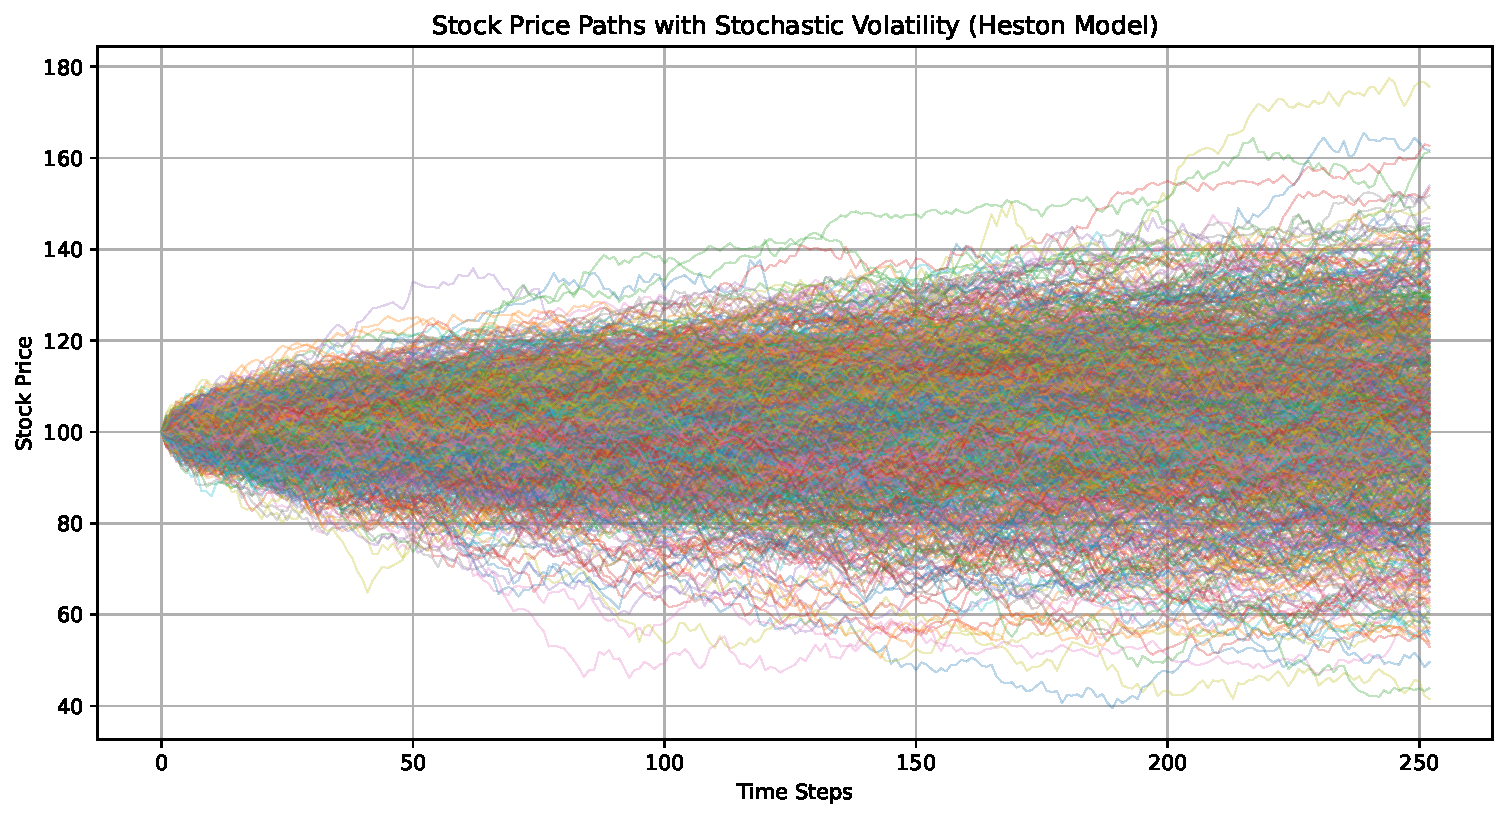
\includegraphics{Chapter5_files/figure-pdf/cell-4-output-1.pdf}

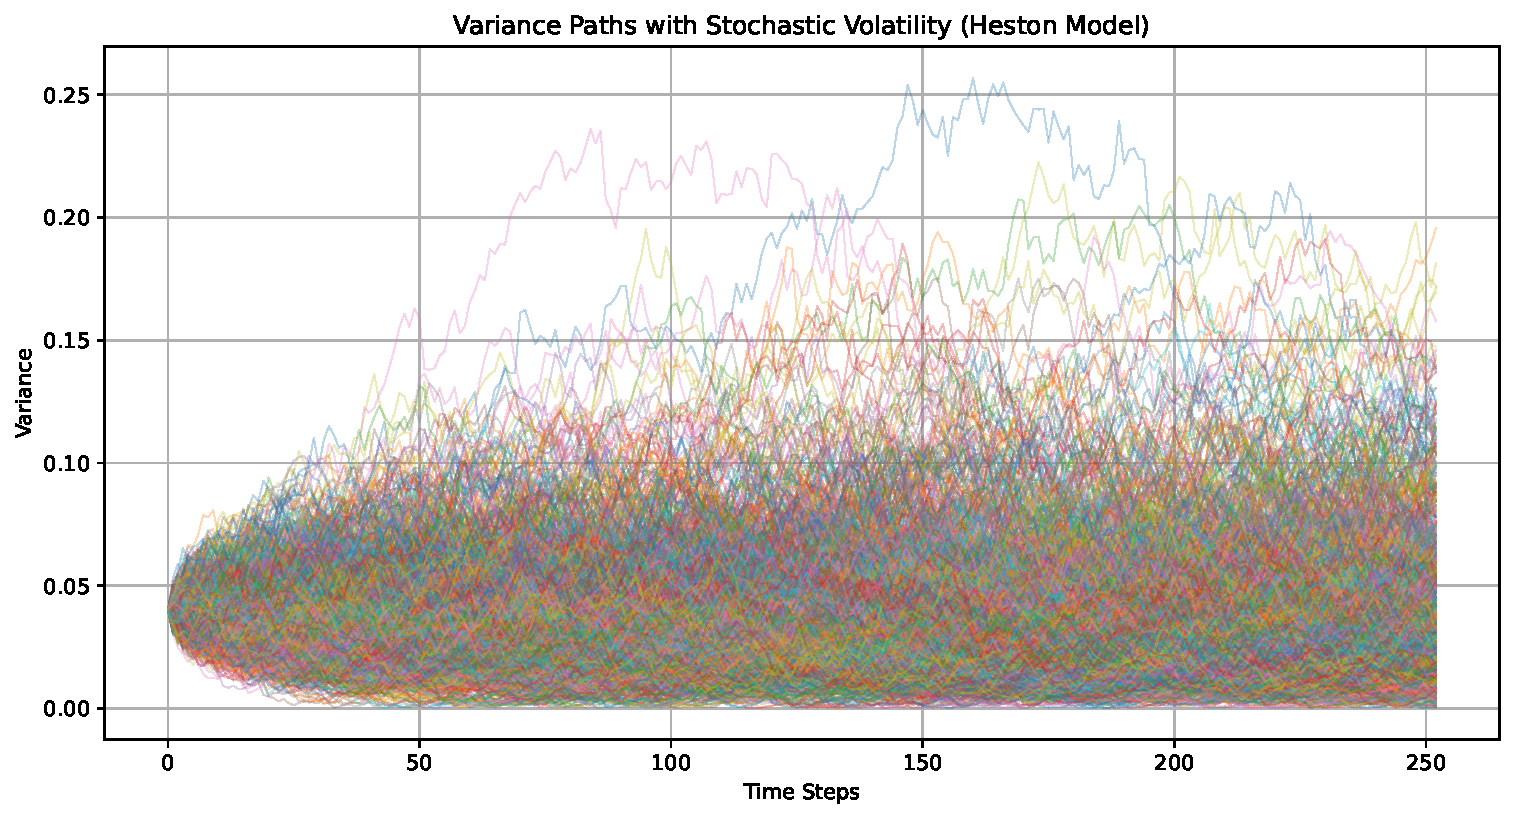
\includegraphics{Chapter5_files/figure-pdf/cell-4-output-2.pdf}

The following code shows that the stock returns under the stochastic
volatility model display fat-tails with positive kurtosis.

\begin{Shaded}
\begin{Highlighting}[]
\ImportTok{import}\NormalTok{ numpy }\ImportTok{as}\NormalTok{ np}
\ImportTok{import}\NormalTok{ pandas }\ImportTok{as}\NormalTok{ pd}
\ImportTok{import}\NormalTok{ matplotlib.pyplot }\ImportTok{as}\NormalTok{ plt}
\ImportTok{import}\NormalTok{ seaborn }\ImportTok{as}\NormalTok{ sns}
\ImportTok{from}\NormalTok{ scipy.stats }\ImportTok{import}\NormalTok{ norm, kurtosis}

\KeywordTok{def}\NormalTok{ simulating\_stochastic\_volatility(S, V0, r, q, dt, N, theta, kappa, sigma, rho, n\_simulations):}
    \CommentTok{"""}
\CommentTok{    Inputs:}
\CommentTok{    S = initial stock price}
\CommentTok{    V0 = initial variance}
\CommentTok{    r = risk{-}free rate}
\CommentTok{    q = dividend yield}
\CommentTok{    dt = length of each time period (Delta t)}
\CommentTok{    N = number of time periods}
\CommentTok{    theta = long{-}term variance (mean of variance)}
\CommentTok{    kappa = rate of mean reversion of variance}
\CommentTok{    sigma = volatility of variance}
\CommentTok{    rho = correlation between the two Wiener processes}
\CommentTok{    n\_simulations = number of simulations}
\CommentTok{    """}
\NormalTok{    LogS }\OperatorTok{=}\NormalTok{ np.log(S)}
\NormalTok{    Sqrdt }\OperatorTok{=}\NormalTok{ np.sqrt(dt)}
    
\NormalTok{    log\_returns }\OperatorTok{=}\NormalTok{ []}
    
    \ControlFlowTok{for}\NormalTok{ \_ }\KeywordTok{in} \BuiltInTok{range}\NormalTok{(n\_simulations):}
\NormalTok{        stock\_price }\OperatorTok{=}\NormalTok{ S}
\NormalTok{        variance }\OperatorTok{=}\NormalTok{ V0}
        \ControlFlowTok{for}\NormalTok{ \_ }\KeywordTok{in} \BuiltInTok{range}\NormalTok{(N):}
\NormalTok{            Z1 }\OperatorTok{=}\NormalTok{ np.random.randn()}
\NormalTok{            Z2 }\OperatorTok{=}\NormalTok{ np.random.randn()}
\NormalTok{            W1 }\OperatorTok{=}\NormalTok{ Z1}
\NormalTok{            W2 }\OperatorTok{=}\NormalTok{ rho }\OperatorTok{*}\NormalTok{ Z1 }\OperatorTok{+}\NormalTok{ np.sqrt(}\DecValTok{1} \OperatorTok{{-}}\NormalTok{ rho}\OperatorTok{**}\DecValTok{2}\NormalTok{) }\OperatorTok{*}\NormalTok{ Z2}
            
\NormalTok{            log\_return }\OperatorTok{=}\NormalTok{ (r }\OperatorTok{{-}}\NormalTok{ q }\OperatorTok{{-}} \FloatTok{0.5} \OperatorTok{*}\NormalTok{ variance) }\OperatorTok{*}\NormalTok{ dt }\OperatorTok{+}\NormalTok{ np.sqrt(variance }\OperatorTok{*}\NormalTok{ dt) }\OperatorTok{*}\NormalTok{ W1}
\NormalTok{            LogS }\OperatorTok{=}\NormalTok{ np.log(stock\_price) }\OperatorTok{+}\NormalTok{ log\_return}
\NormalTok{            stock\_price }\OperatorTok{=}\NormalTok{ np.exp(LogS)}
            
\NormalTok{            variance }\OperatorTok{=}\NormalTok{ np.maximum(variance }\OperatorTok{+}\NormalTok{ kappa }\OperatorTok{*}\NormalTok{ (theta }\OperatorTok{{-}}\NormalTok{ variance) }\OperatorTok{*}\NormalTok{ dt }\OperatorTok{+}\NormalTok{ sigma }\OperatorTok{*}\NormalTok{ np.sqrt(variance }\OperatorTok{*}\NormalTok{ dt) }\OperatorTok{*}\NormalTok{ W2, }\DecValTok{0}\NormalTok{)}
            
\NormalTok{            log\_returns.append(log\_return)}
    
    \ControlFlowTok{return}\NormalTok{ log\_returns}

\CommentTok{\# Example usage:}
\NormalTok{S }\OperatorTok{=} \DecValTok{100}       \CommentTok{\# Initial stock price}
\NormalTok{V0 }\OperatorTok{=} \FloatTok{0.04}     \CommentTok{\# Initial variance}
\NormalTok{r }\OperatorTok{=} \FloatTok{0.05}      \CommentTok{\# Risk{-}free rate}
\NormalTok{q }\OperatorTok{=} \FloatTok{0.02}      \CommentTok{\# Dividend yield}
\NormalTok{dt }\OperatorTok{=} \DecValTok{1}\OperatorTok{/}\DecValTok{252}    \CommentTok{\# Length of each time period (daily)}
\NormalTok{N }\OperatorTok{=} \DecValTok{252}       \CommentTok{\# Number of time periods (one year)}
\NormalTok{theta }\OperatorTok{=} \FloatTok{0.04}  \CommentTok{\# Long{-}term variance}
\NormalTok{kappa }\OperatorTok{=} \FloatTok{0.2}   \CommentTok{\# Rate of mean reversion of variance}
\NormalTok{sigma }\OperatorTok{=} \FloatTok{0.3}   \CommentTok{\# Volatility of variance}
\NormalTok{rho }\OperatorTok{=} \OperatorTok{{-}}\FloatTok{0.7}    \CommentTok{\# Correlation between the two Wiener processes}
\NormalTok{n\_simulations }\OperatorTok{=} \DecValTok{1000}  \CommentTok{\# Number of simulations}

\NormalTok{log\_returns }\OperatorTok{=}\NormalTok{ simulating\_stochastic\_volatility(S, V0, r, q, dt, N, theta, kappa, sigma, rho, n\_simulations)}

\CommentTok{\# Plotting the distribution of log returns}
\NormalTok{sns.histplot(log\_returns, bins}\OperatorTok{=}\DecValTok{100}\NormalTok{, kde}\OperatorTok{=}\VariableTok{True}\NormalTok{, stat}\OperatorTok{=}\StringTok{"density"}\NormalTok{, color}\OperatorTok{=}\StringTok{"blue"}\NormalTok{, label}\OperatorTok{=}\StringTok{"Simulated Log Returns"}\NormalTok{)}
\NormalTok{xmin, xmax }\OperatorTok{=}\NormalTok{ plt.xlim()}
\NormalTok{x }\OperatorTok{=}\NormalTok{ np.linspace(xmin, xmax, }\DecValTok{100}\NormalTok{)}
\NormalTok{p }\OperatorTok{=}\NormalTok{ norm.pdf(x, np.mean(log\_returns), np.std(log\_returns))}
\NormalTok{plt.plot(x, p, }\StringTok{\textquotesingle{}k\textquotesingle{}}\NormalTok{, linewidth}\OperatorTok{=}\DecValTok{2}\NormalTok{, label}\OperatorTok{=}\StringTok{"Normal Distribution"}\NormalTok{)}
\NormalTok{plt.title(}\StringTok{\textquotesingle{}Distribution of Log Returns with Stochastic Volatility\textquotesingle{}}\NormalTok{)}
\NormalTok{plt.xlabel(}\StringTok{\textquotesingle{}Log Return\textquotesingle{}}\NormalTok{)}
\NormalTok{plt.ylabel(}\StringTok{\textquotesingle{}Density\textquotesingle{}}\NormalTok{)}
\NormalTok{plt.legend()}

\CommentTok{\# Display kurtosis}
\NormalTok{kurt }\OperatorTok{=}\NormalTok{ kurtosis(log\_returns)}
\NormalTok{plt.figtext(}\FloatTok{0.15}\NormalTok{, }\FloatTok{0.8}\NormalTok{, }\SpecialStringTok{f\textquotesingle{}Kurtosis: }\SpecialCharTok{\{}\NormalTok{kurt}\SpecialCharTok{:.2f\}}\SpecialStringTok{\textquotesingle{}}\NormalTok{, fontsize}\OperatorTok{=}\DecValTok{12}\NormalTok{)}

\NormalTok{plt.show()}
\end{Highlighting}
\end{Shaded}

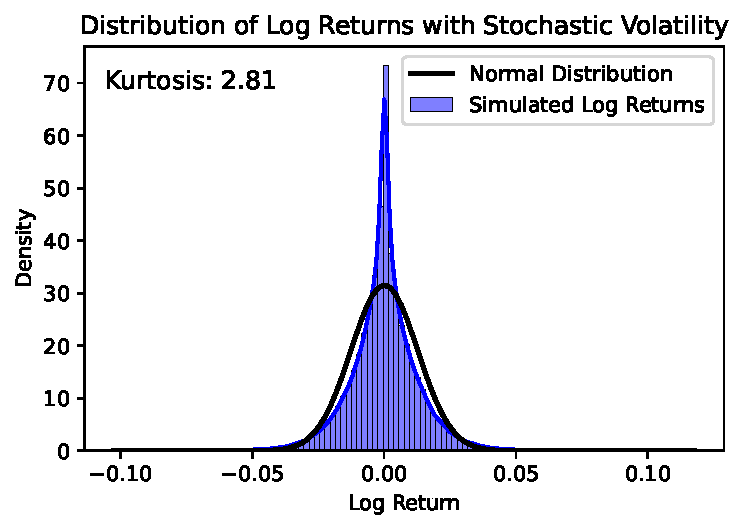
\includegraphics{Chapter5_files/figure-pdf/cell-5-output-1.pdf}

To price European options, we again need to compute
\[\text{prob}^S(S(T)>K) \qquad \text{and} \qquad \text{prob}^R(S(T)>K)\; .\]
The virtue of modelling volatility as in Equation~\ref{eq-heston2} is
that these probabilities can be computed quite efficiently, as shown by
Heston (Heston 1993).\footnote{Further discussion can be found in Epps
  (Epps 2000).} There are many other ways in which one could model
volatility, but the computations may be more difficult. For example, one
could replace Equation~\ref{eq-heston2} by
\begin{equation}\phantomsection\label{eq-heston5}{
\sigma(t) = \mathrm{e}^{v(t)} \quad \text{and} \quad dv(t) = \kappa (\theta-v(t))\,\mathrm{d} t + \lambda \,\mathrm{d} B^*\;.
}\end{equation}

This implies a lognormal volatility and is simpler to simulate than
Equation~\ref{eq-heston2}---because \(\mathrm{e}^{v}\) is well defined
even when \(v\) is negative---but it is easier to calculate the
probabilities \(\text{prob}^S(S(T)>K)\) and \(\text{prob}^R(S(T)>K)\) if
we assume Equation~\ref{eq-heston2}.

One way to implement the GARCH or stochastic volatility model is to
imply both the initial volatility \(\sigma(0)\) and the constants
\(\kappa\), \(\theta\) and \(\lambda\) or \(\kappa\), \(\theta\),
\(\gamma\) and \(\rho\) from observed option prices. These four (or
five) constants can be computed by forcing the model prices of four (or
five) options to equal the observed market prices. Or, a larger set of
prices can be used and the constants can be chosen to minimize the
average squared error or some other measure of goodness-of-fit between
the model and market prices.

\section{Jump Diffusion Models}\label{sec-s_jumpdiffusion}

In the classical Black-Scholes model, stock prices are assumed to follow
a geometric Brownian motion, which is characterized by continuous paths
and normally distributed returns. While this model has been widely used
due to its simplicity and analytical tractability, it fails to capture
certain empirical phenomena observed in financial markets, such as
sudden and significant price changes (jumps) and the heavy tails of
return distributions.

To address these shortcomings, the jump diffusion model was introduced
by Robert C. Merton in 1976. This model extends the Black-Scholes
framework by incorporating jumps into the stock price dynamics, thereby
allowing for discontinuous price paths. The jump diffusion model is
better suited to describe the behavior of financial assets that exhibit
sudden price changes due to news, earnings announcements, or other
market events.

In a jump diffusion model, the stock price \(S_t\) is governed by the
following stochastic differential equation (SDE):

\[
dS_t = \mu S_t \, dt + \sigma S_t \, dW_t + S_t \, dJ_t
\]

where \(\mu\) is the drift rate, \(\sigma\) is the volatility, \(B_t\)
is a standard Brownian motion, \(J_t\) is a jump process.

The jump process \(J_t\) is typically modeled as a compound Poisson
process:

\[
J_t = \sum_{i=1}^{N_t} (Y_i - 1)
\]

where \(N_t\) is a Poisson process with intensity \(\lambda\), \(Y_i\)
are i.i.d. random variables representing the relative jump sizes, with
\(Y_i - 1\) being the actual jump size.

The jump diffusion model introduces several important implications for
the behavior of stock prices and the pricing of derivative securities:

\begin{enumerate}
\def\labelenumi{\arabic{enumi}.}
\tightlist
\item
  \textbf{Heavy Tails}: The inclusion of jumps leads to a return
  distribution with heavier tails compared to the normal distribution,
  aligning better with empirical observations.
\item
  \textbf{Volatility Smile}: The model can generate implied volatility
  smiles, where implied volatility varies with strike price and
  maturity, a feature commonly observed in market data.
\item
  \textbf{Risk Management}: Understanding the jump component is crucial
  for risk management, as it affects the likelihood of extreme price
  movements and the potential for large losses.
\end{enumerate}

The following python code simulates the stock price that evolves as a
jump diffusion.

\begin{Shaded}
\begin{Highlighting}[]
\ImportTok{import}\NormalTok{ numpy }\ImportTok{as}\NormalTok{ np}
\ImportTok{import}\NormalTok{ matplotlib.pyplot }\ImportTok{as}\NormalTok{ plt}

\KeywordTok{def}\NormalTok{ simulate\_jump\_diffusion(S0, mu, sigma, lamb, m, delta, T, N):}
    \CommentTok{"""}
\CommentTok{    Simulate a jump diffusion process.}
\CommentTok{    }
\CommentTok{    Parameters:}
\CommentTok{    S0     : float {-} initial stock price}
\CommentTok{    mu     : float {-} drift rate}
\CommentTok{    sigma  : float {-} volatility}
\CommentTok{    lamb   : float {-} intensity of the Poisson process}
\CommentTok{    m      : float {-} mean of the jump size distribution}
\CommentTok{    delta  : float {-} standard deviation of the jump size distribution}
\CommentTok{    T      : float {-} total time}
\CommentTok{    N      : int   {-} number of time steps}
\CommentTok{    }
\CommentTok{    Returns:}
\CommentTok{    t      : numpy array {-} time points}
\CommentTok{    S      : numpy array {-} simulated stock prices}
\CommentTok{    """}
\NormalTok{    dt }\OperatorTok{=}\NormalTok{ T }\OperatorTok{/}\NormalTok{ N}
\NormalTok{    t }\OperatorTok{=}\NormalTok{ np.linspace(}\DecValTok{0}\NormalTok{, T, N }\OperatorTok{+} \DecValTok{1}\NormalTok{)}
\NormalTok{    S }\OperatorTok{=}\NormalTok{ np.zeros(N }\OperatorTok{+} \DecValTok{1}\NormalTok{)}
\NormalTok{    S[}\DecValTok{0}\NormalTok{] }\OperatorTok{=}\NormalTok{ S0}
    
    \ControlFlowTok{for}\NormalTok{ i }\KeywordTok{in} \BuiltInTok{range}\NormalTok{(}\DecValTok{1}\NormalTok{, N }\OperatorTok{+} \DecValTok{1}\NormalTok{):}
\NormalTok{        Z }\OperatorTok{=}\NormalTok{ np.random.normal(}\DecValTok{0}\NormalTok{, }\DecValTok{1}\NormalTok{)  }\CommentTok{\# Normal random variable for the diffusion part}
\NormalTok{        J }\OperatorTok{=}\NormalTok{ np.random.poisson(lamb }\OperatorTok{*}\NormalTok{ dt)  }\CommentTok{\# Poisson random variable for jumps}
        
        \CommentTok{\# Sum of log{-}normal distributed jumps}
\NormalTok{        Y }\OperatorTok{=}\NormalTok{ np.}\BuiltInTok{sum}\NormalTok{(np.random.normal(m, delta, J))}
        
        \CommentTok{\# Update stock price}
\NormalTok{        S[i] }\OperatorTok{=}\NormalTok{ S[i }\OperatorTok{{-}} \DecValTok{1}\NormalTok{] }\OperatorTok{*}\NormalTok{ np.exp((mu }\OperatorTok{{-}} \FloatTok{0.5} \OperatorTok{*}\NormalTok{ sigma }\OperatorTok{**} \DecValTok{2}\NormalTok{) }\OperatorTok{*}\NormalTok{ dt }\OperatorTok{+}\NormalTok{ sigma }\OperatorTok{*}\NormalTok{ np.sqrt(dt) }\OperatorTok{*}\NormalTok{ Z }\OperatorTok{+}\NormalTok{ Y)}
    
    \ControlFlowTok{return}\NormalTok{ t, S}

\CommentTok{\# Parameters}
\NormalTok{S0 }\OperatorTok{=} \DecValTok{100}         \CommentTok{\# Initial stock price}
\NormalTok{mu }\OperatorTok{=} \FloatTok{0.1}         \CommentTok{\# Drift rate}
\NormalTok{sigma }\OperatorTok{=} \FloatTok{0.2}      \CommentTok{\# Volatility}
\NormalTok{lamb }\OperatorTok{=} \FloatTok{0.75}      \CommentTok{\# Intensity of the Poisson process (average number of jumps per unit time)}
\NormalTok{m }\OperatorTok{=} \FloatTok{0.02}         \CommentTok{\# Mean of the jump size distribution (log{-}normal)}
\NormalTok{delta }\OperatorTok{=} \FloatTok{0.1}      \CommentTok{\# Standard deviation of the jump size distribution (log{-}normal)}
\NormalTok{T }\OperatorTok{=} \FloatTok{1.0}          \CommentTok{\# Total time (1 year)}
\NormalTok{N }\OperatorTok{=} \DecValTok{1000}         \CommentTok{\# Number of time steps}

\CommentTok{\# Simulate the jump diffusion process}
\NormalTok{t, S }\OperatorTok{=}\NormalTok{ simulate\_jump\_diffusion(S0, mu, sigma, lamb, m, delta, T, N)}

\CommentTok{\# Plot the simulated stock prices}
\NormalTok{plt.figure(figsize}\OperatorTok{=}\NormalTok{(}\DecValTok{10}\NormalTok{, }\DecValTok{6}\NormalTok{))}
\NormalTok{plt.plot(t, S, label}\OperatorTok{=}\StringTok{\textquotesingle{}Jump Diffusion Process\textquotesingle{}}\NormalTok{)}
\NormalTok{plt.title(}\StringTok{\textquotesingle{}Simulated Stock Price using Jump Diffusion Model\textquotesingle{}}\NormalTok{)}
\NormalTok{plt.xlabel(}\StringTok{\textquotesingle{}Time (years)\textquotesingle{}}\NormalTok{)}
\NormalTok{plt.ylabel(}\StringTok{\textquotesingle{}Stock Price\textquotesingle{}}\NormalTok{)}
\NormalTok{plt.legend()}
\NormalTok{plt.grid(}\VariableTok{True}\NormalTok{)}
\NormalTok{plt.show()}
\end{Highlighting}
\end{Shaded}

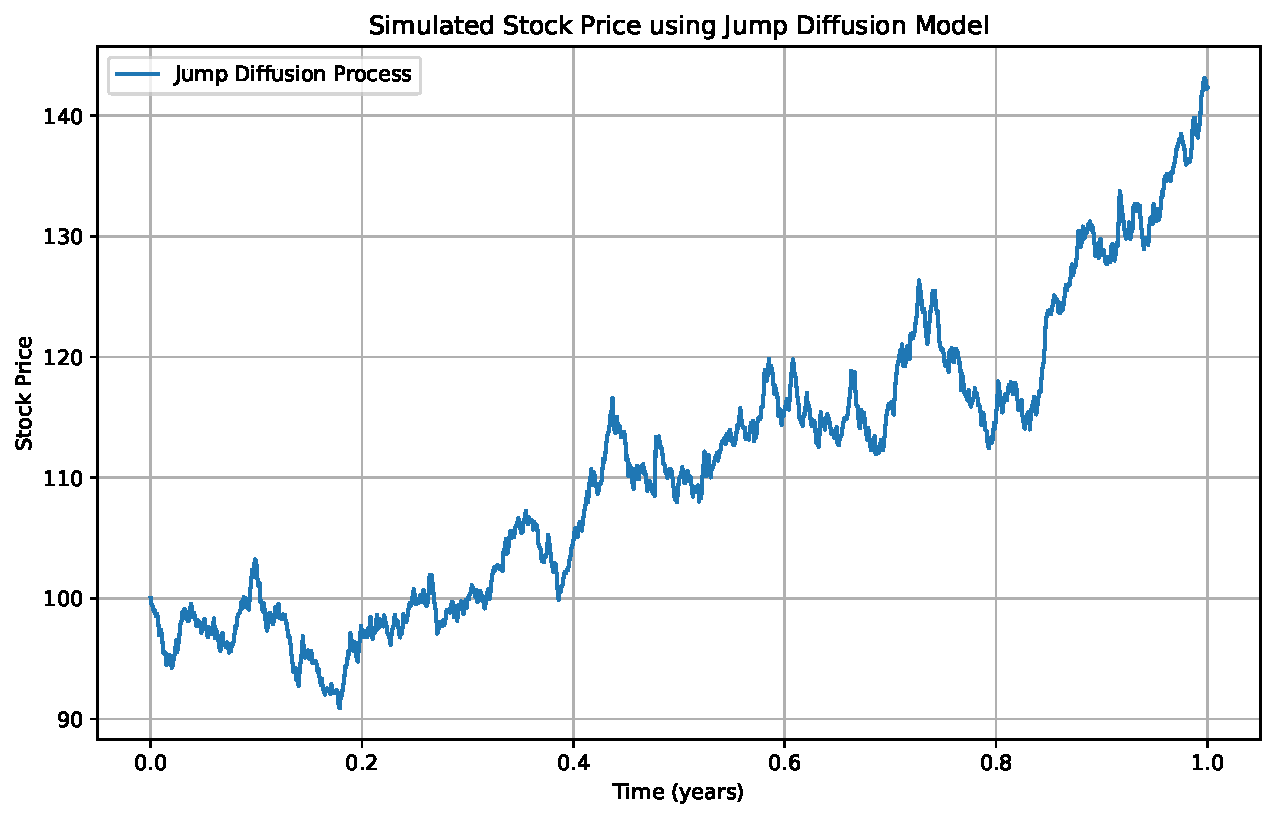
\includegraphics{Chapter5_files/figure-pdf/simulate_jump_diffusion-output-1.pdf}

The jump diffusion model offers a more realistic framework for modeling
stock prices by incorporating the possibility of sudden jumps. This
enhancement over the classical Black-Scholes model allows for better
capturing the empirical characteristics of financial markets, thereby
improving the accuracy of option pricing and risk management practices.

\section{Smiles and Smirks Again}\label{sec-s_smilesagain}

As mentioned before, the GARCH, stochastic volatility and jump diffusion
models can generate fat-tailed distributions for the asset price
\(S(T)\). Thus, they can be more nearly consistent with the option
smiles \index{smile}discussed in Section~\ref{sec-s_smiles} than is the
Black-Scholes model (though it appears that one must include jumps in
asset prices as well as stochastic volatility in order to duplicate
market prices with an option pricing formula). To understand the
relation, let \(\sigma_\text{am}\) denote the implied volatility from an
at-the-money call option, i.e., a call option with strike \(K=S(0)\).
The characteristic of a smile is that implied volatilities from options
of the same maturity with strike prices significantly above and below
\(S(0)\) are higher than \(\sigma_\text{am}\).

A strike price higher than \(S(0)\) corresponds to an out-of-the money
call option. The high implied volatility means that the market is
pricing the right to buy at \(K>S(0)\) above the Black-Scholes price
computed from the volatility \(\sigma_\text{am}\); thus, the market must
attach a higher probability to stock prices \(S(T)>S(0)\) than the
volatility \(\sigma_\text{am}\) would suggest.

A strike price lower than \(S(0)\) corresponds to an in-the-money call
option. The put option with the same strike is out of the money. The
high implied volatility means that the market is pricing call options
above the Black-Scholes price computed from the volatility
\(\sigma_\text{am}\). By put-call parity, the market must also be
pricing put options above the Black-Scholes price computed from the
volatility \(\sigma_\text{am}\). The high prices for the rights to buy
and sell at \(K<S(0)\) means that the market must attach a higher
probability to stock prices \(S(T)<S(0)\) than the volatility
\(\sigma_\text{am}\) would suggest. In particular, the high price for
the right to sell at \(K<S(0)\) means a high insurance premium for
owners of the asset who seek to insure their positions, which is
consistent with a market view that there is a significant probability of
a large loss. This can be interpreted as a crash premium.
\index{crash premium} Indeed, the implied volatilities at strikes less
than \(S(0)\) are typically higher than the implied volatilities at
strikes above \(S(0)\) (giving the smile the appearance of a smirk, as
discussed in Section~\ref{sec-s_smiles}), which is consistent with a
larger probability of crashes than of booms (a fatter tail for low
returns than for high).

As an example, the following code shows that the stochstic volatility
model can generate implied volatility smiles.

This program involes (1) Simulating Heston Model:
simulate\_heston\_paths function generates stock price paths using the
Heston model parameters. (2) Calculating call price by discounting the
averaged call payoffs across the stock price sample paths (3)
Calculating Black Scholes call price : black\_scholes\_call\_price
function calculates the call option price using the Black-Scholes
formula. (4) Calculating implied volatility: implied\_volatility
function computes the implied volatility by solving for the volatility
that matches the Black-Scholes call price to the simulated call price.
(5) Repeating Steps (2)-(4) for different strik prices. (6) Plotting the
implied volatility against strike prices fixing the initial stock price
at \$100.

\begin{Shaded}
\begin{Highlighting}[]
\ImportTok{import}\NormalTok{ numpy }\ImportTok{as}\NormalTok{ np}
\ImportTok{import}\NormalTok{ matplotlib.pyplot }\ImportTok{as}\NormalTok{ plt}
\ImportTok{from}\NormalTok{ scipy.stats }\ImportTok{import}\NormalTok{ norm}
\ImportTok{from}\NormalTok{ scipy.optimize }\ImportTok{import}\NormalTok{ brentq}

\CommentTok{\# Heston model parameters}
\NormalTok{S0 }\OperatorTok{=} \DecValTok{100}      \CommentTok{\# Initial stock price}
\NormalTok{V0 }\OperatorTok{=} \FloatTok{0.04}     \CommentTok{\# Initial variance}
\NormalTok{r }\OperatorTok{=} \FloatTok{0.05}      \CommentTok{\# Risk{-}free rate}
\NormalTok{q }\OperatorTok{=} \FloatTok{0.01}      \CommentTok{\# Dividend yield}
\NormalTok{T }\OperatorTok{=} \DecValTok{1}         \CommentTok{\# Time to maturity (in years)}
\NormalTok{kappa }\OperatorTok{=} \FloatTok{0.25}   \CommentTok{\# Rate of mean reversion of variance}
\NormalTok{theta }\OperatorTok{=} \FloatTok{0.04}  \CommentTok{\# Long{-}term variance}
\NormalTok{sigma }\OperatorTok{=} \FloatTok{0.5}   \CommentTok{\# Volatility of variance}
\NormalTok{rho }\OperatorTok{=} \OperatorTok{{-}}\FloatTok{0.2}    \CommentTok{\# Correlation between the two Wiener processes}
\NormalTok{dt }\OperatorTok{=} \DecValTok{1}\OperatorTok{/}\DecValTok{252}    \CommentTok{\# Length of each time period (daily)}
\NormalTok{N }\OperatorTok{=} \DecValTok{252}       \CommentTok{\# Number of time periods (one year)}
\NormalTok{n\_simulations }\OperatorTok{=} \DecValTok{10000}  \CommentTok{\# Number of simulations}

\KeywordTok{def}\NormalTok{ simulate\_heston\_paths(S0, V0, r, q, T, kappa, theta, sigma, rho, dt, N, n\_simulations):}
\NormalTok{    S }\OperatorTok{=}\NormalTok{ np.zeros((N }\OperatorTok{+} \DecValTok{1}\NormalTok{, n\_simulations))}
\NormalTok{    V }\OperatorTok{=}\NormalTok{ np.zeros((N }\OperatorTok{+} \DecValTok{1}\NormalTok{, n\_simulations))}
\NormalTok{    S[}\DecValTok{0}\NormalTok{] }\OperatorTok{=}\NormalTok{ S0}
\NormalTok{    V[}\DecValTok{0}\NormalTok{] }\OperatorTok{=}\NormalTok{ V0}
    
    \ControlFlowTok{for}\NormalTok{ t }\KeywordTok{in} \BuiltInTok{range}\NormalTok{(}\DecValTok{1}\NormalTok{, N }\OperatorTok{+} \DecValTok{1}\NormalTok{):}
\NormalTok{        Z1 }\OperatorTok{=}\NormalTok{ np.random.normal(size}\OperatorTok{=}\NormalTok{n\_simulations)}
\NormalTok{        Z2 }\OperatorTok{=}\NormalTok{ np.random.normal(size}\OperatorTok{=}\NormalTok{n\_simulations)}
\NormalTok{        W1 }\OperatorTok{=}\NormalTok{ Z1}
\NormalTok{        W2 }\OperatorTok{=}\NormalTok{ rho }\OperatorTok{*}\NormalTok{ Z1 }\OperatorTok{+}\NormalTok{ np.sqrt(}\DecValTok{1} \OperatorTok{{-}}\NormalTok{ rho}\OperatorTok{**}\DecValTok{2}\NormalTok{) }\OperatorTok{*}\NormalTok{ Z2}
        
\NormalTok{        V[t] }\OperatorTok{=}\NormalTok{ np.maximum(V[t}\OperatorTok{{-}}\DecValTok{1}\NormalTok{] }\OperatorTok{+}\NormalTok{ kappa }\OperatorTok{*}\NormalTok{ (theta }\OperatorTok{{-}}\NormalTok{ V[t}\OperatorTok{{-}}\DecValTok{1}\NormalTok{]) }\OperatorTok{*}\NormalTok{ dt }\OperatorTok{+}\NormalTok{ sigma }\OperatorTok{*}\NormalTok{ np.sqrt(V[t}\OperatorTok{{-}}\DecValTok{1}\NormalTok{] }\OperatorTok{*}\NormalTok{ dt) }\OperatorTok{*}\NormalTok{ W2, }\DecValTok{0}\NormalTok{)}
\NormalTok{        S[t] }\OperatorTok{=}\NormalTok{ S[t}\OperatorTok{{-}}\DecValTok{1}\NormalTok{] }\OperatorTok{*}\NormalTok{ np.exp((r }\OperatorTok{{-}}\NormalTok{ q }\OperatorTok{{-}} \FloatTok{0.5} \OperatorTok{*}\NormalTok{ V[t}\OperatorTok{{-}}\DecValTok{1}\NormalTok{]) }\OperatorTok{*}\NormalTok{ dt }\OperatorTok{+}\NormalTok{ np.sqrt(V[t}\OperatorTok{{-}}\DecValTok{1}\NormalTok{] }\OperatorTok{*}\NormalTok{ dt) }\OperatorTok{*}\NormalTok{ W1)}
    
    \ControlFlowTok{return}\NormalTok{ S, V}

\KeywordTok{def}\NormalTok{ black\_scholes\_call\_price(S, K, T, r, sigma):}
\NormalTok{    d1 }\OperatorTok{=}\NormalTok{ (np.log(S }\OperatorTok{/}\NormalTok{ K) }\OperatorTok{+}\NormalTok{ (r }\OperatorTok{+} \FloatTok{0.5} \OperatorTok{*}\NormalTok{ sigma}\OperatorTok{**}\DecValTok{2}\NormalTok{) }\OperatorTok{*}\NormalTok{ T) }\OperatorTok{/}\NormalTok{ (sigma }\OperatorTok{*}\NormalTok{ np.sqrt(T))}
\NormalTok{    d2 }\OperatorTok{=}\NormalTok{ d1 }\OperatorTok{{-}}\NormalTok{ sigma }\OperatorTok{*}\NormalTok{ np.sqrt(T)}
\NormalTok{    call\_price }\OperatorTok{=}\NormalTok{ S }\OperatorTok{*}\NormalTok{ norm.cdf(d1) }\OperatorTok{{-}}\NormalTok{ K }\OperatorTok{*}\NormalTok{ np.exp(}\OperatorTok{{-}}\NormalTok{r }\OperatorTok{*}\NormalTok{ T) }\OperatorTok{*}\NormalTok{ norm.cdf(d2)}
    \ControlFlowTok{return}\NormalTok{ call\_price}

\KeywordTok{def}\NormalTok{ implied\_volatility(C, S, K, T, r):}
    \KeywordTok{def}\NormalTok{ objective\_function(sigma):}
        \ControlFlowTok{return}\NormalTok{ black\_scholes\_call\_price(S, K, T, r, sigma) }\OperatorTok{{-}}\NormalTok{ C}
    \ControlFlowTok{try}\NormalTok{:}
        \ControlFlowTok{return}\NormalTok{ brentq(objective\_function, }\FloatTok{0.001}\NormalTok{, }\FloatTok{5.0}\NormalTok{)}
    \ControlFlowTok{except} \PreprocessorTok{ValueError}\NormalTok{:}
        \ControlFlowTok{return}\NormalTok{ np.nan}

\CommentTok{\# Simulate paths using the Heston model}
\NormalTok{S\_paths, \_ }\OperatorTok{=}\NormalTok{ simulate\_heston\_paths(S0, V0, r, q, T, kappa, theta, sigma, rho, dt, N, n\_simulations)}

\CommentTok{\# Calculate option prices at different strike prices}
\NormalTok{strike\_prices }\OperatorTok{=}\NormalTok{ np.linspace(}\DecValTok{90}\NormalTok{, }\DecValTok{120}\NormalTok{, }\DecValTok{20}\NormalTok{)}
\NormalTok{call\_prices }\OperatorTok{=}\NormalTok{ np.zeros\_like(strike\_prices)}

\ControlFlowTok{for}\NormalTok{ i, K }\KeywordTok{in} \BuiltInTok{enumerate}\NormalTok{(strike\_prices):}
\NormalTok{    call\_payoffs }\OperatorTok{=}\NormalTok{ np.maximum(S\_paths[}\OperatorTok{{-}}\DecValTok{1}\NormalTok{] }\OperatorTok{{-}}\NormalTok{ K, }\DecValTok{0}\NormalTok{)}
\NormalTok{    call\_prices[i] }\OperatorTok{=}\NormalTok{ np.mean(call\_payoffs) }\OperatorTok{*}\NormalTok{ np.exp(}\OperatorTok{{-}}\NormalTok{r }\OperatorTok{*}\NormalTok{ T)}

\CommentTok{\# Calculate implied volatilities}
\NormalTok{implied\_vols }\OperatorTok{=}\NormalTok{ [implied\_volatility(C, S0, K, T, r) }\ControlFlowTok{for}\NormalTok{ C, K }\KeywordTok{in} \BuiltInTok{zip}\NormalTok{(call\_prices, strike\_prices)]}

\CommentTok{\# Filter out NaN values that may occur}
\NormalTok{valid\_indices }\OperatorTok{=} \OperatorTok{\textasciitilde{}}\NormalTok{np.isnan(implied\_vols)}
\NormalTok{strike\_prices }\OperatorTok{=}\NormalTok{ strike\_prices[valid\_indices]}
\NormalTok{implied\_vols }\OperatorTok{=}\NormalTok{ np.array(implied\_vols)[valid\_indices]}

\CommentTok{\# Plot the implied volatility smile}
\NormalTok{plt.figure(figsize}\OperatorTok{=}\NormalTok{(}\DecValTok{10}\NormalTok{, }\DecValTok{6}\NormalTok{))}
\NormalTok{plt.plot(strike\_prices, implied\_vols, label}\OperatorTok{=}\StringTok{\textquotesingle{}Implied Volatility\textquotesingle{}}\NormalTok{, marker}\OperatorTok{=}\StringTok{\textquotesingle{}o\textquotesingle{}}\NormalTok{)}
\NormalTok{plt.title(}\StringTok{\textquotesingle{}Implied Volatility Smile\textquotesingle{}}\NormalTok{)}
\NormalTok{plt.xlabel(}\StringTok{\textquotesingle{}Strike Price\textquotesingle{}}\NormalTok{)}
\NormalTok{plt.ylabel(}\StringTok{\textquotesingle{}Implied Volatility\textquotesingle{}}\NormalTok{)}
\NormalTok{plt.legend()}
\NormalTok{plt.grid(}\VariableTok{True}\NormalTok{)}
\NormalTok{plt.show()}
\end{Highlighting}
\end{Shaded}

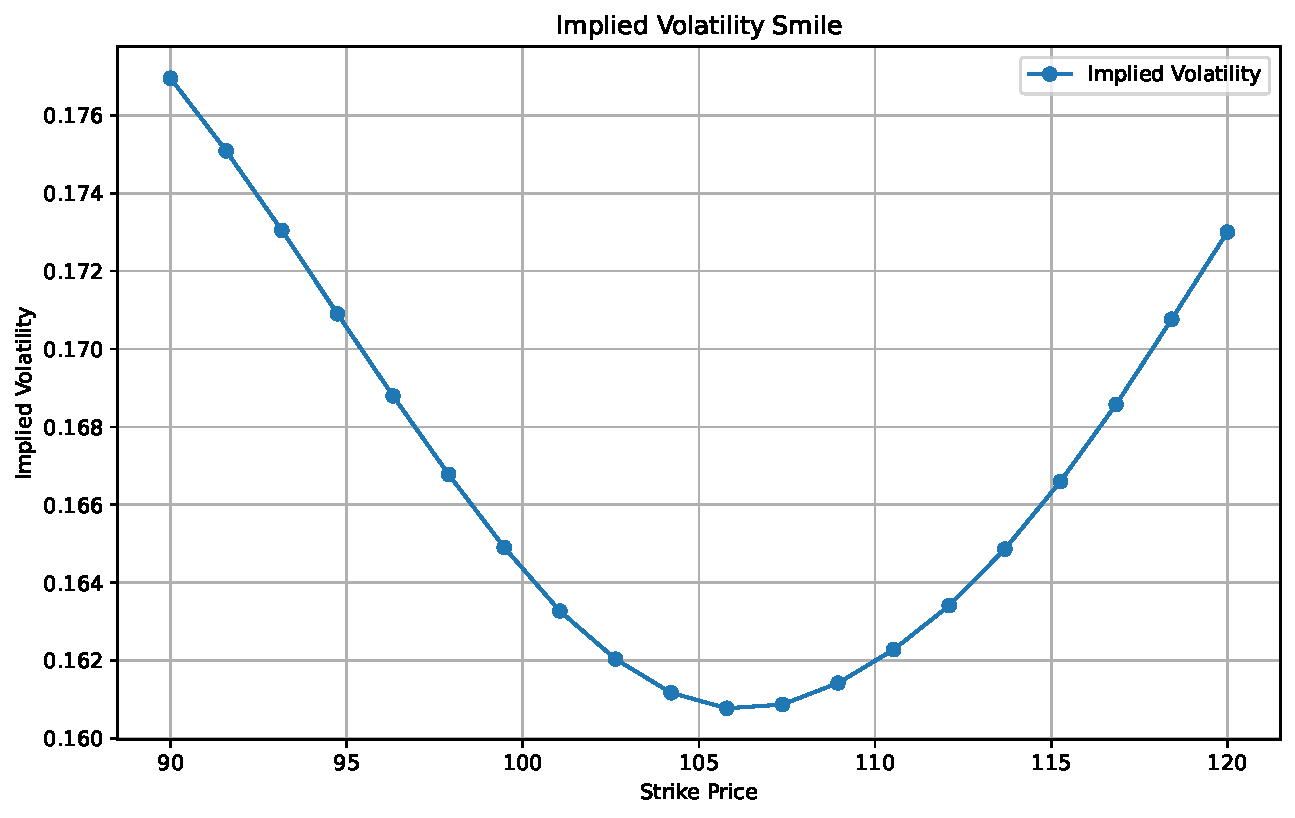
\includegraphics{Chapter5_files/figure-pdf/cell-7-output-1.pdf}

\section{Hedging and Market
Completeness}\label{hedging-and-market-completeness}

The GARCH model is inherently a discrete-time model. If returns have a
GARCH structure at one frequency (e.g., monthly), they will not have a
GARCH structure at a different frequency (e.g., weekly). Hence, the
return period (monthly, weekly, \ldots) is part of the specification of
the model. One interpretation of the model is that the dates \(t_i\) at
which the variance changes are the only dates at which investors can
trade. Under this interpretation, it is impossible to perfectly hedge an
option: the gross return \(S(t_i)/S(t_{i-1})\) over the interval
\((t_{i-1},t_i)\) is lognormally distributed, so no portfolio of the
stock and riskless asset formed at \(t_{i-1}\) and held over the
interval \((t_{i-1},t_i)\) can perfectly replicate the return of an
option over the interval. As discussed in
Section~\ref{sec-s_incomplete}, we call a market in which some
derivatives cannot be perfectly hedged an incomplete market.
\index{incomplete market} Thus, the GARCH model is an example of an
incomplete market, if investors can only trade at the frequency at which
returns have a GARCH structure. However, it is unreasonable to assume
that investors can only trade weekly or monthly or even daily.

Another interpretation of the GARCH model is that investors can trade
continuously and the asset has a constant volatility within each period
\((t_{i-1},t_i)\). Under this interpretation, the market is complete and
options can be delta-hedged. The completeness is a result of the fact
that the change \(\sigma_{i+1}-\sigma_i\) in the volatility at date
\(t_i\) (recall that \(\sigma_i\) is the volatility over the period
\((t_{i-1},t_i)\) and \(\sigma_{i+1}\) is the volatility over the period
\((t_{i},t_{i+1})\)) depends only on \(\log S(t_i)\). Thus, the only
random factor in the model that needs to be hedged is, as usual, the
underlying asset price. However, this interpretation of the model is
also a bit strange. Suppose for example that monthly returns are assumed
to have a GARCH structure. Then the model states that the volatility in
February will be higher if there is an unusually large return (in
absolute value) in January. Suppose there is an unusually large return
in the first half of January. Then, intuitively, one would expect the
change in the volatility to occur in the second half of January rather
than being delayed until February. However, the model specifies that the
volatility is constant during each month, hence constant during January
in this example.

The stochastic volatility model is more straightforward. The market is
definitely incomplete. The value of a call option at date \(t<T\), where
\(T\) is the maturity of the option, will depend on the underlying asset
price \(S(t)\) and the volatility \(\sigma(t)\). Denoting the value by
\(C(t,S(t),\sigma(t))\), we have from Ito's formula that \[
\mathrm{d} C(t) = \text{something}\;\mathrm{d} t + \frac{\partial C}{\partial S}\,\mathrm{d} S(t) + \frac{\partial C}{\partial \sigma}\,\mathrm{d} \sigma(t)\; .\]
A replicating portfolio must have the same dollar change at each date
\(t\). If we hold \(\partial C/\partial S\) shares of the underlying
asset, then the change in the value of the shares will be
\((\partial C/\partial S)\,\mathrm{d} S\). However, there is no way to
match the\\
\((\partial C/\partial \sigma)\,\mathrm{d} \sigma\) term using the
underlying asset and the riskless asset.

The significance of the market being incomplete is that the value of a
derivative asset that cannot be replicated using traded assets (e.g.,
the underlying and riskless assets) is not uniquely determined by
arbitrage considerations. As discussed in
Section~\ref{sec-s_incomplete}, one must use equilibrium pricing in this
circumstance. \index{equilibrium pricing} That is what we have
implicitly done in this chapter. By assuming particular dynamics for the
volatility under the risk-neutral measure, we have implicitly selected a
particular risk-neutral measure from the set of risk-neutral measures
that are consistent with the absence of arbitrage.

\section{Exercises}\label{exercises-3}

\begin{exercise}[]\protect\hypertarget{exr-e_mixture}{}\label{exr-e_mixture}

The purpose of this exercise is to generate a fat-tailed distribution
from a model that is simpler than the GARCH and stochastic volatility
models but has somewhat the same flavor. The distribution will be a
mixture of normals. Create a python program in which the user can input
\(S\), \(r\), \(q\), \(T\), \(\sigma_1\) and \(\sigma_2\). Use these
inputs to produce a column of 500 simulated \(\log S(T)\). In each
simulation, define \(\log S(T)\) as
\[\log S(T) = \log S(0) + \left(r-q-\frac{1}{2}\sigma^2\right)T + \sigma \sqrt{T}z\;,\]
where \(z\) is a standard normal,
\(\sigma = x\sigma_1 + (1-x)\sigma_2\), and \(x\) is a random variable
that equals zero or one with equal probabilities.

Calculate the mean and standard deviation of the \(\log S(T)\) and
calculate the fraction that lie more than two standard deviations below
the mean. If the \(\log S(T)\) all came from a normal distribution with
the same variance, then this fraction should equal \(\mathrm{N}(-2) =\)
2.275\%. If the fraction is higher, then the distribution is fat tailed.
(Of course, the actual fraction would differ from 2.275\% in any
particular case due to the randomness of the simulation, even if all of
the \(\log S(T)\) came from a normal distribution with the same
variance).

\end{exercise}

\begin{exercise}[]\protect\hypertarget{exr-e_GARCH1}{}\label{exr-e_GARCH1}

Create a python program prompting the user to input the same inputs as
in the \texttt{simulating\_garch} function except for the initial
volatility and \(\theta\). Simulate 500 paths of a GARCH process and
output \(\log S(T)\) for each simulation (you don't need to output the
entire paths as in the \texttt{simulating\_garch} function). Take the
initial volatility to be 0.3 and \(\theta = 0.09\). Determine whether
the distribution is fat-tailed by computing the fraction of the
\(\log S(T)\) that lie two or more standard deviations below the mean,
as in the previous exercise. For what values of \(\kappa\) and
\(\lambda\) does the distribution appear to be especially fat-tailed?

\end{exercise}

\begin{exercise}[]\protect\hypertarget{exr-nolabel}{}\label{exr-nolabel}

Repeat Exercise~\ref{exr-e_GARCH1} for the Heston stochastic volatility
model, describing the values of \(\kappa\), \(\gamma\) and \(\rho\) that
appear to generate especially fat-tailed distributions.

\end{exercise}

\bookmarksetup{startatroot}

\chapter{Monte Carlo and Binomial Models}\label{sec-c_introcomputation}

In this chapter, we will introduce two principal numerical methods for
valuing derivative securities: Monte Carlo and binomial models. We will
consider two applications: valuing European options in the presence of
stochastic volatility with Monte Carlo and valuing American options via
binomial models. Additional applications of these methods will be
presented in \textbf{?@sec-c\_montecarlo}. Throughout the chapter, we
will assume there is a constant risk-free rate. The last section, while
quite important, could be skimmed on first reading---the rest of the
book does not build upon it.

\section{Introduction to Monte Carlo}\label{sec-s_mc_europeans}

According to our risk-neutral pricing
Equation~\ref{eq-riskneutralformula}, the value of a security paying an
amount \(x\) at date \(T\) is
\begin{equation}\phantomsection\label{eq-montecarlo1}{
\mathrm{e}^{-rT}E^R[x]\;.
}\end{equation}

To estimate this by Monte-Carlo \index{Monte Carlo} means to simulate a
sample of values for the random variable \(x\) and to estimate the
expectation by averaging the sample values.\footnote{Boyle\textasciitilde{}(Boyle
  1977) introduced Monte-Carlo methods for derivative valuation,
  including the variance-reduction methods of control variates and
  antithetic variates to be discussed in \textbf{?@sec-c\_montecarlo}}.
Of course, for this to work, the sample must be generated from a
population having a distribution consistent with the risk-neutral
probabilities.

The simplest example is valuing a European option under the
Black-Scholes assumptions. Of course, for calls and puts, this is
redundant, because we already have the Black-Scholes formulas.
Nevertheless, we will describe how to do this for the sake of
introducing the Monte Carlo method. In the case of a call option, the
random variable \(x\) in Equation~\ref{eq-montecarlo1} is
\(\max(0,S(T)-K)\). To simulate a sample of values for this random
variable, we need to simulate the terminal stock price \(S(T)\). This is
easy to do, because, under the Black-Scholes assumptions, the logarithm
of \(S(T)\) is normally distributed under the risk-neutral measure with
mean \(\log S(0)+\mathrm{n}u T\) and variance \(\sigma^2T\), where
\(\mathrm{n}u=r-q-\sigma^2/2\). Thus, we can simulate values for
\(\log S(T)\) as \(\log S(0)+\mathrm{n}u T + \sigma\sqrt{T}z\), where
\(z\) is a standard normal. We can average the simulated values of
\(\max(0,S(T)-K)\), or whatever the payoff of the derivative is, and
then discount at the risk-free rate to compute the date--0 value of the
derivative. This means that we generate some number \(M\) of standard
normals \(z_i\) and estimate the option value as
\(\mathrm{e}^{-rT}\bar{x}\), where \(\bar{x}\) is the mean of
\[x_i = \max\left(0,\mathrm{e}^{\log S(0)+\mathrm{n}u T + \sigma\sqrt{T}z_i}-K\right)\; .\]
To value options that are path-dependent we need to simulate the path of
the underlying asset price. Path-dependent options are discussed in
Chaps.\textasciitilde{}\ref{c_exotics}
and\textasciitilde{}\ref{c_montecarlo}.

There are two main drawbacks to Monte-Carlo methods. First, it is
difficult (though not impossible) to value early-exercise
features.\footnote{Monte-Carlo methods for valuing early exercise
  include the stochastic mesh method of Broadie and Glasserman (Broadie
  and Glasserman 1997) and the regression method of Longstaff and
  Schwartz (Longstaff and Schwartz 2001). Glasserman (Glasserman 2004)
  provides a good discussion of these methods and the relation between
  them.} To value early exercise, we need to know the value at each date
if not exercised, to compare to the intrinsic value. One could consider
performing a simulation at each date to calculate the value if not
exercised, but this value depends on the option to exercise early at
later dates, which cannot be calculated without knowing the value of
being able to exercise early at even later dates, etc. In contrast, the
binomial model (and finite difference models discussed in
Chapter~\ref{sec-c_pde}) can easily handle early exercise but cannot
easily handle path dependencies.

The second drawback of Monte Carlo methods is that they can be quite
inefficient in terms of computation time (though, as will be explained
in \textbf{?@sec-c\_montecarlo}, they may be faster than alternative
methods for derivatives written on multiple assets). As in statistics,
the standard error of the estimate depends on the sample size.
Specifically, we observed in Section~\ref{sec-s_statistics} that, given
a random sample \(\{x_1,\ldots,x_M\}\) of size \(M\) from a population
with mean \(\mu\) and variance \(\sigma^2\), the best estimate of
\(\mu\) is the sample mean \(\bar{x}\), and the standard error of
\(\bar{x}\) (which means the standard deviation of \(\bar{x}\) in
repeated samples) is best estimated by
\begin{equation}\phantomsection\label{eq-standarderror}{
\sqrt{\frac{1}{M(M-1)}\left(\sum_{i=1}^{M} x_i^2-M\bar{x}^2\right)}\;.
}\end{equation} \index{standard error} Recall that \(\bar{x}\) plus or
minus 1.96 standard errors is a 95\% confidence interval for \(\mu\)
when the \(x_i\) are normally distributed. In the context of European
option valuation, the expression Equation~\ref{eq-standarderror} gives
the standard error of the estimated option value at maturity, and
multiplication of Equation~\ref{eq-standarderror} by
\(\mathrm{e}^{-rT}\) gives the standard error of the estimated date--0
option value.

To obtain an estimate with an acceptably small standard error may
require a large sample size and hence a relatively large amount of
computation time. The complexities of Monte Carlo methods arise from
trying to reduce the required sample size. In
\textbf{?@sec-c\_montecarlo}, we will describe two such methods
(antithetic variates and control variates). For those who want to engage
in a more detailed study of Monte Carlo methods, the book of Glasserman
(Glasserman 2004) is highly recommended. J"ackel (Jäckel 2002) is useful
for more advanced readers, and Clewlow and Strickland (Clewlow and
Strickland 1998) and Brandimarte (Brandimarte 2002) are useful
references that include computer code.

\subsection{Monte Carlo Valuation of a European
Call}\label{monte-carlo-valuation-of-a-european-call}

We will illustrate Monte Carlo by valuing a European call under the
Black-Scholes assumptions. We will also estimate the delta by each of
the methods described in Section~\ref{sec-s_montecarlogreeks1}
and\textasciitilde{}\ref{s_montecarlogreeks2}. Of course, we know the
call value and its delta from the Black-Scholes formulas, and they can
be used to evaluate the accuracy of the Monte Carlo estimates. We use
the code in Chapter (\textbf{\#sec-c\_continuoustime?}). In this
circumstance, we only need to simulate the price of the underlying at
the option maturity rather than the entire path of the price process.
Therefore we set \(m=1\). However, we use a large number of paths,
\(n=10000\) to get a large sample of terminal stock prices.

\begin{Shaded}
\begin{Highlighting}[]
\CommentTok{\# Simulate Geometric Brownian Motion}
\ImportTok{import}\NormalTok{ numpy }\ImportTok{as}\NormalTok{ np}
\ImportTok{import}\NormalTok{ matplotlib.pyplot }\ImportTok{as}\NormalTok{ plt}
\CommentTok{\# number of paths}
\NormalTok{n }\OperatorTok{=} \DecValTok{10000}
\CommentTok{\#number of divisions}
\NormalTok{m }\OperatorTok{=} \DecValTok{1}
\CommentTok{\# Interest rate (We set the drift equal to the interest rate for the risk neutral measure)}
\NormalTok{r }\OperatorTok{=} \FloatTok{0.1}
\CommentTok{\# Volatility}
\NormalTok{sig }\OperatorTok{=} \FloatTok{0.2}
\CommentTok{\# Initial Stock Price}
\NormalTok{S0 }\OperatorTok{=} \DecValTok{42}
\CommentTok{\# Maturity}
\NormalTok{T }\OperatorTok{=} \FloatTok{0.5}
\CommentTok{\#Strike Price}
\NormalTok{K}\OperatorTok{=}\DecValTok{40}
\CommentTok{\# Dividend Yield}
\NormalTok{q}\OperatorTok{=}\FloatTok{0.0}
\CommentTok{\# Delta t}
\NormalTok{dt }\OperatorTok{=}\NormalTok{ T}\OperatorTok{/}\NormalTok{m}
\CommentTok{\# Drift}
\NormalTok{drift }\OperatorTok{=}\NormalTok{ (r}\OperatorTok{{-}}\NormalTok{q}\OperatorTok{{-}}\FloatTok{0.5}\OperatorTok{*}\NormalTok{sig}\OperatorTok{**}\DecValTok{2}\NormalTok{)}
\CommentTok{\# Volatility}
\NormalTok{vol }\OperatorTok{=}\NormalTok{ sig }\OperatorTok{*}\NormalTok{ np.sqrt(dt)}

\NormalTok{t }\OperatorTok{=}\NormalTok{ np.array(}\BuiltInTok{range}\NormalTok{(}\DecValTok{0}\NormalTok{,m }\OperatorTok{+} \DecValTok{1}\NormalTok{,}\DecValTok{1}\NormalTok{)) }\OperatorTok{*}\NormalTok{ dt}

\CommentTok{\# seed for random generator}
\NormalTok{seed}\OperatorTok{=} \DecValTok{2020}
\CommentTok{\# define a random generator}
\NormalTok{np.random.seed(seed)}
\NormalTok{inc }\OperatorTok{=}\NormalTok{ np.zeros(shape }\OperatorTok{=}\NormalTok{ (m }\OperatorTok{+} \DecValTok{1}\NormalTok{, n))}
\NormalTok{inc[}\DecValTok{1}\NormalTok{:] }\OperatorTok{=}\NormalTok{ np.transpose(np.random.normal(loc }\OperatorTok{=} \DecValTok{0}\NormalTok{, scale }\OperatorTok{=}\NormalTok{ vol,size }\OperatorTok{=}\NormalTok{ (n,m)))}
\NormalTok{St }\OperatorTok{=}\NormalTok{ np.zeros(shape }\OperatorTok{=}\NormalTok{ (m }\OperatorTok{+} \DecValTok{1}\NormalTok{, n))}
\NormalTok{St }\OperatorTok{=}\NormalTok{ S0 }\OperatorTok{*}\NormalTok{ np.exp(np.cumsum(inc,axis}\OperatorTok{=}\DecValTok{0}\NormalTok{) }\OperatorTok{+}\NormalTok{ (drift }\OperatorTok{*}\NormalTok{ t[}\DecValTok{0}\NormalTok{:m }\OperatorTok{+} \DecValTok{1}\NormalTok{])[:,}\VariableTok{None}\NormalTok{])}
\NormalTok{St1 }\OperatorTok{=}\NormalTok{ S0 }\OperatorTok{*}\NormalTok{ np.exp(}\OperatorTok{{-}}\NormalTok{np.cumsum(inc,axis}\OperatorTok{=}\DecValTok{0}\NormalTok{) }\OperatorTok{+}\NormalTok{ (drift }\OperatorTok{*}\NormalTok{ t[}\DecValTok{0}\NormalTok{:m }\OperatorTok{+} \DecValTok{1}\NormalTok{])[:,}\VariableTok{None}\NormalTok{])}
\end{Highlighting}
\end{Shaded}

As before, this code generates two samples \(St\), which adds the
simulated standard (zero mean) normal random variable, and \(St1\) which
subtracts the simulated (zero mean) standard normal random variable.
Each sample produces and estimate for the Black-Scholes European call
option.

\begin{Shaded}
\begin{Highlighting}[]
\NormalTok{cc}\OperatorTok{=}\NormalTok{np.maximum(St[m,:]}\OperatorTok{{-}}\NormalTok{K,}\DecValTok{0}\NormalTok{)}
\NormalTok{cp }\OperatorTok{=}\NormalTok{ np.mean(cc) }\OperatorTok{*}\NormalTok{ np.exp(}\OperatorTok{{-}}\NormalTok{r }\OperatorTok{*}\NormalTok{ T)}
\NormalTok{cc1}\OperatorTok{=}\NormalTok{np.maximum(St1[m,:]}\OperatorTok{{-}}\NormalTok{K,}\DecValTok{0}\NormalTok{)}\OperatorTok{*}\NormalTok{np.exp(}\OperatorTok{{-}}\NormalTok{r }\OperatorTok{*}\NormalTok{ T)}
\NormalTok{cp1}\OperatorTok{=}\NormalTok{ np.mean(np.maximum(St1[m,:]}\OperatorTok{{-}}\NormalTok{K,}\DecValTok{0}\NormalTok{)) }\OperatorTok{*}\NormalTok{ np.exp(}\OperatorTok{{-}}\NormalTok{r }\OperatorTok{*}\NormalTok{ T)}

\BuiltInTok{print}\NormalTok{(}\StringTok{\textquotesingle{}The first sample gives an estimated call price=\textquotesingle{}}\NormalTok{,cp)}
\BuiltInTok{print}\NormalTok{(}\StringTok{\textquotesingle{}The second sample gives an estimated call price=\textquotesingle{}}\NormalTok{,cp1)}
\NormalTok{bsc }\OperatorTok{=}\NormalTok{ (cp}\OperatorTok{+}\NormalTok{cp1)}\OperatorTok{/}\DecValTok{2}
\BuiltInTok{print}\NormalTok{(}\StringTok{\textquotesingle{}The average of the two estimates=\textquotesingle{}}\NormalTok{,bsc)}
\end{Highlighting}
\end{Shaded}

\begin{verbatim}
The first sample gives an estimated call price= 4.791646287615179
The second sample gives an estimated call price= 4.687624646438364
The average of the two estimates= 4.739635467026771
\end{verbatim}

The true call price is given by

\begin{Shaded}
\begin{Highlighting}[]
\ImportTok{from}\NormalTok{ scipy }\ImportTok{import}\NormalTok{ stats}
\ImportTok{import}\NormalTok{ numpy }\ImportTok{as}\NormalTok{ np}
\ImportTok{from}\NormalTok{ scipy.optimize }\ImportTok{import}\NormalTok{ minimize, minimize\_scalar}

\KeywordTok{def}\NormalTok{ blackscholes(S0, K, r, q, sig, T, call }\OperatorTok{=} \VariableTok{True}\NormalTok{):}
    \CommentTok{\textquotesingle{}\textquotesingle{}\textquotesingle{}Calculate option price using B{-}S formula.}
\CommentTok{    }
\CommentTok{    Args:}
\CommentTok{        S0 (num): initial price of underlying asset.}
\CommentTok{        K (num): strick price.}
\CommentTok{        r (num): risk free rate}
\CommentTok{        q (num): dividend yield}
\CommentTok{        sig (num): Black{-}Scholes volatility.}
\CommentTok{        T (num): maturity.}
\CommentTok{        call (bool): True returns call price, False returns put price.}
\CommentTok{        }
\CommentTok{    Returns:}
\CommentTok{        num}
\CommentTok{    \textquotesingle{}\textquotesingle{}\textquotesingle{}}
\NormalTok{    d1 }\OperatorTok{=}\NormalTok{ (np.log(S0}\OperatorTok{/}\NormalTok{K) }\OperatorTok{+}\NormalTok{ (r }\OperatorTok{{-}}\NormalTok{q }\OperatorTok{+}\NormalTok{ sig}\OperatorTok{**}\DecValTok{2}\OperatorTok{/}\DecValTok{2}\NormalTok{) }\OperatorTok{*}\NormalTok{ T)}\OperatorTok{/}\NormalTok{(sig}\OperatorTok{*}\NormalTok{np.sqrt(T))}
\NormalTok{    d2 }\OperatorTok{=}\NormalTok{ d1 }\OperatorTok{{-}}\NormalTok{ sig}\OperatorTok{*}\NormalTok{np.sqrt(T)}
 \CommentTok{\#    \textless{}!{-}{-} norm = sp.stats.norm {-}{-}\textgreater{}}
\NormalTok{    norm }\OperatorTok{=}\NormalTok{ stats.norm}
    \ControlFlowTok{if}\NormalTok{ call:}
        \ControlFlowTok{return}\NormalTok{ np.exp(}\OperatorTok{{-}}\NormalTok{ q }\OperatorTok{*}\NormalTok{T) }\OperatorTok{*}\NormalTok{ S0 }\OperatorTok{*}\NormalTok{ norm.cdf(d1,}\DecValTok{0}\NormalTok{,}\DecValTok{1}\NormalTok{) }\OperatorTok{{-}}\NormalTok{ K }\OperatorTok{*}\NormalTok{ np.exp(}\OperatorTok{{-}}\NormalTok{r }\OperatorTok{*}\NormalTok{ T) }\OperatorTok{*}\NormalTok{ norm.cdf(d2,}\DecValTok{0}\NormalTok{, }\DecValTok{1}\NormalTok{) }
    \ControlFlowTok{else}\NormalTok{:}
        \ControlFlowTok{return} \OperatorTok{{-}}\NormalTok{np.exp(}\OperatorTok{{-}}\NormalTok{q }\OperatorTok{*}\NormalTok{ T) }\OperatorTok{*}\NormalTok{ S0 }\OperatorTok{*}\NormalTok{ norm.cdf(}\OperatorTok{{-}}\NormalTok{d1,}\DecValTok{0}\NormalTok{,}\DecValTok{1}\NormalTok{) }\OperatorTok{+}\NormalTok{ K }\OperatorTok{*}\NormalTok{ np.exp(}\OperatorTok{{-}}\NormalTok{r }\OperatorTok{*}\NormalTok{ T) }\OperatorTok{*}\NormalTok{ norm.cdf(}\OperatorTok{{-}}\NormalTok{d2,}\DecValTok{0}\NormalTok{, }\DecValTok{1}\NormalTok{)}

\NormalTok{truebsc}\OperatorTok{=}\NormalTok{blackscholes(S0, K, r, q, sig, T, call }\OperatorTok{=} \VariableTok{True}\NormalTok{)}
\BuiltInTok{print}\NormalTok{(}\StringTok{\textquotesingle{}The black scholes fromula=\textquotesingle{}}\NormalTok{,truebsc)}
\end{Highlighting}
\end{Shaded}

\begin{verbatim}
The black scholes fromula= 4.759422392871532
\end{verbatim}

Notice that even with 10000 data points for each sample the individual
estimates are not very accurate compared to the exact Black Scoles
price. This is a well known problem that is difficult to estimate the
mean, even with a lot of data and is a drawback to Monte Carlo as
discussed earlier. However, the average of the two prices is
sgnificantly more accurate. This is an example of an antithetic variable
which is discussed later. One simple intution is the two samples yield
negatively correlated errors; if the plus sample is two high, then the
minus sample will be too low. Combined, the simulation error will cancel
out. Another intution is that each individual sample has a wrong
estimate of the mean. However, the combined sample has zero mean by
construction. Therefore combining the samples give the right mean of the
simulated standard normal random variable. Nevertheless, there is still
sampling error since we are estimating the mean of the discounted call
payoffs, not the mean of the standard normal. This method and other
methods to reduce sampling error are discussed next.

\#\# Antithetic Variates in Monte Carlo

In this and the following section, we will discuss two methods to
increase the efficiency of the Monte Carlo method. These are two of the
simplest methods. They are used extensively, but there are other
important methods that are also widely used. J"ackel (Jäckel 2002) and
Glasserman (Glasserman 2004) provide a wealth of information on this
topic.

The Monte Carlo method estimates the mean \(\mu\) of a random variable
\(x\) as the sample average of randomly generated values of \(x\). An
antithetic variate \index{antithetic variate} is a random variable \(y\)
with the same mean as \(x\) and a negative correlation with \(x\). It
follows that the random variable \(z=(x+y)/2\) will have the same mean
as \(x\) and a lower variance. Therefore the sample mean of \(M\)
simulations of \(z\) will be an unbiased estimate of \(\mu\) and will
have a lower standard error than the sample mean of \(M\) simulations of
\(x\). Thus, we should obtain a more efficient estimator of \(\mu\) by
simulating \(z\) instead of \(x\).\footnote{ The negative correlation
  between \(x\) and \(y\) is essential for this method to generate a
  real gain in efficiency. To generate \(M\) simulations of \(z\), one
  must generate \(M\) simulations of \(x\) and \(M\) of \(y\), which
  will generally require about as much computation time as generating
  \(2M\) simulations of \(x\). If \(x\) and \(y\) were independent, the
  standard error from \(M\) simulations of \(z\) would be the same as
  the standard error from \(2M\) simulations of \(x\), so using the
  antithetic variate would be no better than just doubling the sample
  size for \(x\).}

In the context of derivative valuation, the standard application of this
idea is to generate two negatively correlated underlying asset prices
(or price paths, if the derivative is path dependent). The terminal
value of the derivative written on the first asset serves as \(x\) and
the terminal value of the derivative written on the second serves as
\(y\). Because both asset prices have the same distribution, the means
of \(x\) and \(y\) will be the same, and the discounted mean is the
date--0 value of the derivative.

Consider for example a non-path-dependent option in a world with
constant volatility. In each simulation \(i\) (\(i=1,\ldots,M\)), we
would generate a standard normal \(Z_i\) and compute \begin{align*}
\log S_i(T) &= \log S(0) + \left(r-q-\frac{1}{2}\sigma^2\right)T + \sigma\sqrt{T}Z_i\; ,\\
\log S_i'(T) &= \log S(0) + \left(r-q-\frac{1}{2}\sigma^2\right)T - \sigma\sqrt{T}Z_i\;.
\end{align*} Given the first terminal price, the value of the derivative
will be some number \(x_i\) and given the second it will be some number
\(y_i\). The date--0 value of the derivative is estimated as
\[\mathrm{e}^{-rT}\frac{1}{M}\sum_{i=1}^M\frac{x_i+y_i}{2}\; .\]

\section{Control Variates in Monte Carlo}\label{sec-s_controlvariates}

\index{control variate} Another approach to increasing the efficiency of
the Monte Carlo method is to adjust the estimated mean (option value)
based on the known mean of another related variable. We can explain this
in terms of linear regression in statistics. Suppose we have a random
sample \(\{x_1,\ldots,x_M\}\) of a variable \(x\) with unknown mean
\(\mu\), and suppose we have a corresponding sample
\(\{y_1,\ldots,y_M\}\) of another variable \(y\) with known mean
\(\phi\). Then an efficient estimate of \(\mu\) is
\(\hat{\mu} = \bar{x} + \hat{\beta} (\phi-\bar{y})\), where \(\bar{x}\)
and \(\bar{y}\) denote the sample means of \(x\) and \(y\), and where
\(\hat{\beta}\) is the coefficient of \(y\) in the linear regression of
\(x\) on \(y\) (i.e., the estimate of \(\beta\) in the linear model
\(x = \alpha +\beta y + \varepsilon\)). The standard Monte Carlo method,
which we have described thus far, simply estimates the mean of \(x\) as
\(\bar{x}\). The control variate method adjusts the estimate by adding
\(\hat{\beta} (\phi-\bar{y})\). To understand this correction, assume
for example that the true \(\beta\) is positive. If the random sample is
such that \(\bar{y}<\phi\), then it must be that small values of \(y\)
were over-represented in the sample. Since \(x\) and \(y\) tend to move
up and down together (this is the meaning of a positive \(\beta\)) it is
likely that small values of \(x\) were also over-represented in the
sample. Therefore, one should adjust the sample mean of \(x\) upwards in
order to estimate \(\mu\). The best adjustment will take into account
the extent to which small values of \(y\) were over-represented (i.e.,
the difference between \(\bar{y}\) and \(\phi\)) and the strength of the
relation between \(x\) and \(y\) (which the estimate \(\hat{\beta}\)
represents). The efficient correction of this sort is also the simplest:
just add \(\hat{\beta}(\phi-\bar{y})\) to \(\bar{x}\). In practice, the
estimation of \(\hat{\beta}\) may be omitted and one may simply take
\(\hat{\beta}=1\), if the relationship between \(x\) and \(y\) can be
assumed to be one-for-one. If \(\beta\) is to be estimated, the estimate
(by ordinary least squares) is
\[\hat{\beta} = \frac{\sum_{i=1}^M x_iy_i - M\bar{x}\bar{y}}{\sum_{i=1}^M y_i^2 - M\bar{y}^2}\; .\]
In general, the correction term \(\hat{\beta}(\phi-\bar{y})\) will have
a nonzero mean, which introduces a bias in the estimate of \(\mu\). To
eliminate the bias, one can compute \(\hat{\beta}\) from a pre-sample of
\(\{x,y\}\) values.

As an example of a control variate, in our simulation code to estimate
the Black Scholes price for a call option we can use the stock price
itself. The known stock price is the inout price \(S0\). The simulation
also produces an estimate for the stock price as the dicsounted expected
value of the terminal stock price
\(\hat{S}=\sum_{i=1}^{n} e^{- r T } St(m,i)\) where \(St(m,i)\) is the
\(i\)th simulated stock price at time \(T\). Theoretically these should
be the same umber, but due to error they typically wil not be the same.

\begin{Shaded}
\begin{Highlighting}[]
\NormalTok{SS}\OperatorTok{=}\NormalTok{np.mean(St[m,:])}\OperatorTok{*}\NormalTok{np.exp(}\OperatorTok{{-}}\NormalTok{r}\OperatorTok{*}\NormalTok{T)}
\BuiltInTok{print}\NormalTok{(}\StringTok{\textquotesingle{}The Estimated Stock Price for the first sample is =\textquotesingle{}}\NormalTok{, SS)}
\BuiltInTok{print}\NormalTok{(}\StringTok{\textquotesingle{}The actual stock price should be=\textquotesingle{}}\NormalTok{, S0)}
\BuiltInTok{print}\NormalTok{(}\StringTok{\textquotesingle{}The error is =\textquotesingle{}}\NormalTok{, S0}\OperatorTok{{-}}\NormalTok{SS)}
\end{Highlighting}
\end{Shaded}

\begin{verbatim}
The Estimated Stock Price for the first sample is = 42.05899999577932
The actual stock price should be= 42
The error is = -0.058999995779316805
\end{verbatim}

The error is \(S0-\hat{S}\) which corresponds to \(\phi-y\) above. We
then compute \(\hat{\beta}\) and comute the improved estimate
\[ \text{new estimate}= \text{original estimate} +\hat{\beta}(S0-\hat{S}) \]
In the code below we do this procedure for both samples and average the
updates.

\begin{Shaded}
\begin{Highlighting}[]
\NormalTok{hatbeta}\OperatorTok{=}\NormalTok{ np.cov(St[m,:],cc)[}\DecValTok{0}\NormalTok{,}\DecValTok{1}\NormalTok{]}\OperatorTok{/}\NormalTok{np.cov(St[m,],cc)[}\DecValTok{1}\NormalTok{,}\DecValTok{1}\NormalTok{]}
\NormalTok{hatbeta1}\OperatorTok{=}\NormalTok{np.cov(St1[m,:],cc1)[}\DecValTok{0}\NormalTok{,}\DecValTok{1}\NormalTok{]}\OperatorTok{/}\NormalTok{np.cov(St1[m,],cc1)[}\DecValTok{1}\NormalTok{,}\DecValTok{1}\NormalTok{]}
\NormalTok{correction }\OperatorTok{=}\NormalTok{hatbeta}\OperatorTok{*}\NormalTok{(S0}\OperatorTok{{-}}\NormalTok{SS)}
\NormalTok{update}\OperatorTok{=}\NormalTok{cp }\OperatorTok{+}\NormalTok{ correction}
\BuiltInTok{print}\NormalTok{(}\StringTok{\textquotesingle{}hatbeta=\textquotesingle{}}\NormalTok{,hatbeta)}
\BuiltInTok{print}\NormalTok{(}\StringTok{\textquotesingle{}The original estimate for the call price from the first sample=\textquotesingle{}}\NormalTok{,cp)}
\BuiltInTok{print}\NormalTok{(}\StringTok{\textquotesingle{}The original estimate for the call price from the second sample=\textquotesingle{}}\NormalTok{,cp1)}
\BuiltInTok{print}\NormalTok{(}\StringTok{\textquotesingle{}The updated estimate from the first sample is=\textquotesingle{}}\NormalTok{,update)}
\NormalTok{SS1}\OperatorTok{=}\NormalTok{np.mean(St1[m,:])}\OperatorTok{*}\NormalTok{np.exp(}\OperatorTok{{-}}\NormalTok{r}\OperatorTok{*}\NormalTok{T)}
\NormalTok{update1}\OperatorTok{=}\NormalTok{cp1}\OperatorTok{+}\NormalTok{hatbeta1}\OperatorTok{*}\NormalTok{(S0}\OperatorTok{{-}}\NormalTok{SS1)}
\BuiltInTok{print}\NormalTok{(}\StringTok{\textquotesingle{}The updated estimate from the second sample is=\textquotesingle{}}\NormalTok{,update1)}
\BuiltInTok{print}\NormalTok{(}\StringTok{\textquotesingle{}The average of the updated estimates =\textquotesingle{}}\NormalTok{,(update}\OperatorTok{+}\NormalTok{update1)}\OperatorTok{/}\DecValTok{2}\NormalTok{)}
\end{Highlighting}
\end{Shaded}

\begin{verbatim}
hatbeta= 1.1541186403411716
The original estimate for the call price from the first sample= 4.791646287615179
The original estimate for the call price from the second sample= 4.687624646438364
The updated estimate from the first sample is= 4.723553292706219
The updated estimate from the second sample is= 4.780385012196883
The average of the updated estimates = 4.751969152451551
\end{verbatim}

We can compare this to the exact Black Scholes formula from before.

\begin{Shaded}
\begin{Highlighting}[]
\BuiltInTok{print}\NormalTok{(}\StringTok{\textquotesingle{}The exact Black Scholes Price is=\textquotesingle{}}\NormalTok{, truebsc)}
\end{Highlighting}
\end{Shaded}

\begin{verbatim}
The exact Black Scholes Price is= 4.759422392871532
\end{verbatim}

As another example, consider the classic case of estimating the value of
a discretely-sampled average-price call, using a discretely-sampled
geometric-average-price call \index{average-price option}
\index{geometric-average option} as a control variate. Let \(\tau\)
denote the amount of time that has elapsed since the call was issued and
\(T\) the amount of time remaining before maturity, so the total
maturity of the call is \(T+\tau\). To simplify somewhat, assume date 0
is the beginning of a period between observations. Let
\(t_1, \ldots, t_N\) denote the remaining sampling dates, with
\(t_1 = \Delta t\), \(t_i-t_{i-1}=\Delta t = T/N\) for each \(i\), and
\(t_N=T\). We will input the average price \(A(0)\) computed up to date
0, assuming this average includes the price \(S(0)\) at date 0. The
average price at date \(T\) will be
\[A(T) = \frac{\tau}{T+\tau}A(0) + \frac{T}{T+\tau}\left(\frac{\sum_{i=1}^N S(t_i)}{N}\right)\; .\]
The average-price call pays \(\max(0,A(T)-K)\) at its maturity \(T\),
and we can write this as \begin{align*}
\max(A(T)-K,0) &= \max\left(\frac{T}{T+\tau}\left( \frac{\sum_{i=1}^N S(t_i)}{N}\right) - \left(K - \frac{\tau}{T+\tau}A(0)\right), 0\right)\\
&= \frac{T}{T+\tau} \max \left(\frac{\sum_{i=1}^N S(t_i)}{N} - K^*,0\right)\;,
\end{align*} where \[K^* = \frac{T+\tau}{T}K - \frac{\tau}{T}A(0)\; .\]
Therefore, the value at date 0 of the discretely-sampled average-price
call is
\[\frac{T}{T+\tau} \,\mathrm{e}^{-rT} E^R\left[\max \left(\frac{\sum_{i=1}^N S(t_i)}{N} - K^*,0\right)\right]\; .\]
In terms of the discussion above, the random variable the mean of which
we want to estimate is
\[x = \mathrm{e}^{-rT}\max \left(\frac{\sum_{i=1}^N S(t_i)}{N} - K^*,0\right)\; .\]
A random variable \(y\) that will be closely correlated to \(x\) is
\[y =\mathrm{e}^{-rT}\max \left(\mathrm{e}^{\sum_{i=1}^N \log S(t_i)/N} - K^*,0\right)\; .\]
The mean \(\phi\) of \(y\) under the risk-neutral measure is given in
the pricing Equation~\ref{eq-disc_geom_avg_call}. We can use the sample
mean of \(y\) and its known mean \(\phi\) to adjust the sample mean of
\(x\) as an estimator of the value of the average-price call. Generally,
the estimated adjustment coefficient \(\hat{\beta}\) will be quite close
to 1.

\section{Monte Carlo Greeks I: Difference
Ratios}\label{sec-s_montecarlogreeks1}

Greeks can be calculated by Monte Carlo by running the valuation program
twice and computing a difference ratio, for example
\((C_u-C_d)/(S_u-S_d)\) to estimate a delta. However, to minimize the
error, and minimize the number of computations required, one should use
the same set of random draws to estimate the derivative value for
different values of the parameter. For path-independent options (e.g.,
European puts and calls) under the Black-Scholes assumptions, we only
need to generate \(S(T)\) and then we can compute \(S_u(T)\) as
\([S_u(0)/S(0)] \times S(T)\) and \(S_d(T)\) as
\([S_u(0)/S(0)] \times S(T)\). We can estimate standard errors for the
Greeks in the same way that we estimate the standard error of the
derivative value.

Actually, there is often a better method available that is just as
simple. This is called pathwise calculation. We will explain this in the
next section. Here we will describe how to estimate the delta and gamma
of a derivative as sample means of difference ratios.

Consider initial prices for the underlying \(S_u>S>S_d\). Denote the
underlying price at the option maturity in a given simulation by
\(S_u(T)\) when the initial underlying price is \(S_u\), by \(S(T)\)
when the initial underlying price is \(S\), and by \(S_d(T)\) when the
initial underlying price is \(S_d\). Under the Black-Scholes
assumptions, the logarithm of the stock price at date \(T\) starting
from the three initial prices \(S_d\), \(S\) and \(S_u\) is
\begin{align*}
\log S_d(T) &= \log S_d + \left(r-q-\frac{1}{2}\sigma^2\right)T + \sigma B(T)\; ,\\
\log S(T) &= \log S + \left(r-q-\frac{1}{2}\sigma^2\right)T + \sigma B(T)\; ,\\
\log S_u (T) &= \log S_u + \left(r-q-\frac{1}{2}\sigma^2\right)T + \sigma B(T)\;,
\end{align*} so
\[\log S_d(T) = \log S(T) + \log S_d - \log S\Longrightarrow S_d(T) = \left(\frac{S_d}{S}\right) S(T)\; ,\]
and
\[\log S_u(T) = \log S(T) + \log S_u - \log S \Longrightarrow S_u(T) = \left(\frac{S_u}{S}\right) S(T)\; .\]
Therefore, under the Black-Scholes assumptions, we only need to simulate
\(S(T)\) and then perform the multiplications indicated above to obtain
\(S_d(T)\) and \(S_u(T)\).

Consider a particular simulation and let \(C_d(T)\) denote the value of
the derivative at maturity when the initial asset price is \(S_d\), let
\(C(T)\) denote the value of the derivative at maturity when the initial
asset price is \(S\), and let \(C_u(T)\) denote the value of the
derivative at maturity when the initial asset price is \(S_u\). For
path-independent derivatives under the Black-Scholes assumptions, these
can be computed directly from the simulation of \(S(T)\) as just
described. However, the following applies to general European
derivatives under general assumptions about the underlying asset price
(for example, it could follow a GARCH process).

The estimates \(C_d\), \(C\) and \(C_u\) of the date--0 derivative
values, for the different initial prices of the underlying, are the
discounted sample means of the \(C_d(T)\), \(C(T)\) and \(C_u(T)\). One
way to estimate the delta is \((C_u-C_d)/(S_u-S_d)\). This is a
difference of discounted sample means, multiplied by the reciprocal of
\(S_u-S_d\). Equivalently, it is the sample mean of the differences
\(C_u(T)-C_d(T)\), multiplied by \(\mathrm{e}^{-rT}/(S_u-S_d)\). As a
sample mean, its standard error can be estimated as described in
Chapter~\ref{sec-c_stochasticvolatility}. The standard error is
\[\frac{\mathrm{e}^{-rT}}{S_u-S_d}\sqrt{\frac{1}{M(M-1)}\left(\sum_{i=1}^M \left[C_{ui}(T)-C_{di}(T)\right]^2 - M\left[\overline{C_{u}(T)}-\overline{C_{d}(T)}\right]^2\right)}\; ,\]
\index{standard error} where the overline denotes the sample mean and
where \(C_{ui}(T)\) {[}respectively, \(C_{di}(T)\){]} denotes the value
of the derivative at maturity in simulation \(i\) when the initial asset
price is \(S_u\) {[}respectively, \(S_d\){]}.

The corresponding Monte Carlo estimate of the gamma is also a sample
mean. Simple algebra shows that Equation~\ref{eq-binomialgamma100} is
equivalent to
\begin{equation}\phantomsection\label{eq-binomialgamma200}{
\Gamma = \frac{2}{(S_u-S)(S_u-S_d)}C_u - \frac{2}{(S_u-S)(S-S_d)}C +\frac{2}{(S-S_d)(S_u-S_d)}C_d\;.
}\end{equation}

Normally one would take \(S_u=(1+\alpha)S\) and \(S_d = (1-\alpha)S\)
for some \(\alpha\) (e.g., \(\alpha=0.01\)). In this case
Equation~\ref{eq-binomialgamma200} simplifies to
\begin{equation}\phantomsection\label{eq-binomialgamma300}{
\Gamma = \frac{C_u - 2C + C_d}{\alpha^2S^2}\;,
}\end{equation}

and the standard error of the gamma is

\begin{multline*}\frac{\mathrm{e}^{-rT}}{\alpha^2S^2}\sqrt{\frac{1}{M(M-1)}}\\
\times \sqrt{\sum_{i=1}^M \left[C_{ui}(T)-2C_i(T)+C_{di}(T)\right]^2 -M\left[\overline{C_{u}(T)}-2\overline{C(T)}+\overline{C_{d}(T)}\right]^2}\; .
\end{multline*}

\section{Monte Carlo Greeks II: Pathwise
Estimates}\label{sec-s_montecarlogreeks2}

We will examine the bias in the Monte Carlo delta estimate discussed in
the preceding section and explain pathwise estimation of Greeks. By
biased, we mean that the expected value of an estimate is different from
the true value. \index{bias} It is important to recognize that if a
Monte Carlo estimate is biased, then, even if a large number of
simulations is used and the standard error is nearly zero, the answer
provided by the Monte Carlo method will be incorrect. For simplicity,
consider a European call under the Black-Scholes assumptions.

The delta estimate we have considered is the discounted sample mean of
\begin{equation}\phantomsection\label{eq-montecarlodelta2}{
\frac{C_u(T) - C_d(T)}{S_u-S_d}\;.}\end{equation}

This ratio takes on one of three values, depending on \(S(T)\):

\begin{itemize}
\tightlist
\item
  If \(S_u(T) \leq K\) then the option is out of the money in both the
  up and down cases; i.e., \[C_u(T) = C_d(T) = 0\; ,\] so the ratio
  Equation~\ref{eq-montecarlodelta2} is zero.
\item
  If \(S_d(T) \geq K\) then the option is in the money in both the up
  and down cases; i.e.,
  \begin{align*} C_u(T) &= S_u(T) - K =\left(\frac{S_u}{S}\right)S(T) - K\; ,\\
  C_d(T) &= S_d(T) - K = \left(\frac{S_d}{S}\right)S(T) - K\;,
  \end{align*} so the ratio Equation~\ref{eq-montecarlodelta2} equals
  \(S(T)/S\).
\item
  If \(S_u(T) > K > S_d(T)\), then the option is in the money in only
  the up case; i.e., \begin{align*}
  C_u(T) &= S_u(T) - K = \left(\frac{S_u}{S}\right)S(T) - K\; ,\\
  C_d(T) &= 0\;,
  \end{align*} so the ratio Equation~\ref{eq-montecarlodelta2} equals
  \[\frac{\left(\frac{S_u}{S}\right)S(T) - K}{S_u-S_d} < \frac{S(T)}{S}\; .\]
\end{itemize}

The bias is induced by the third case above. We can see this as follows.
We are trying to estimate
\begin{equation}\phantomsection\label{eq-montecarlodelta4}{
\frac{\partial }{\partial S} \mathrm{e}^{-rT}E^R \big[\max(0,S(T)-K)\big] = \mathrm{e}^{-rT}E^R  \left[ \frac{\partial }{\partial S} \max(0,S(T)-K)\right]\;.
}\end{equation}

The delta estimate \((C_u-C_d)/(S_u-S_d)\) replaces the mean \(E^R\)
with the sample mean and replaces
\begin{equation}\phantomsection\label{eq-montecarlodelta3}{
\frac{\partial }{\partial S} \max(0,S(T)-K)
}\end{equation}

with the ratio Equation~\ref{eq-montecarlodelta2}. The derivative
Equation~\ref{eq-montecarlodelta3} takes on two possible values,
depending on \(S(T)\)---we can ignore the case \(S(T)=K\) because it
occurs with zero probability:

\begin{itemize}
\tightlist
\item
  If \(S(T) < K\), then \(\max(0,S(T)-K) = 0\) and the derivative is
  zero.
\item
  If \(S(T)>K\), then \(\max(0,S(T)-K) = S(T)-K\) and the derivative
  equals
  \[\frac{\partial S(T)}{\partial S}=\mathrm{e}^{(r-q-\sigma^2/2)T + \sigma B(T)} = \frac{S(T)}{S}\; .\]
\end{itemize}

Therefore, the true delta---the expectation
Equation~\ref{eq-montecarlodelta4}---equals\footnote{By changing
  numeraires, we can show that Equation~\ref{eq-montecarlodelta5} equals
  \(\mathrm{e}^{-qT}E^V[x] = \mathrm{e}^{-qT}\mathrm{N}(d_1)\), as we
  know from Chapter~\ref{sec-c_blackscholes} is the delta of a European
  call in the Black-Scholes model (here, as in
  Chapter~\ref{sec-c_blackscholes}, \(V(t)=\mathrm{e}^{qt}S(t)\) denotes
  the value of the non-dividend-paying portfolio created from the
  stock).} \begin{equation}\phantomsection\label{eq-montecarlodelta5}{
\mathrm{e}^{-rT}E^R\left[\frac{S(T)}{S} x\right]\;,
}\end{equation}

where \(x\) is the random variable defined as \begin{equation*}
x =  \begin{cases} 1 & \text{if $S(T)>K$}\; ,\\
0 & \text{otherwise}\;.
\end{cases}
\end{equation*} On the other hand, our analysis of the ratio
Equation~\ref{eq-montecarlodelta2} shows that the expected value of the
delta estimate \((C_u-C_d)/(S_u-S_d)\) is
\begin{equation}\phantomsection\label{eq-montecarlodelta6}{
\mathrm{e}^{-rT}E^R\left[\frac{S(T)}{S} y\right] + \mathrm{e}^{-rT}E^R\left[\frac{S_uS(T)-SK}{S(S_u-S_d)}z\right]\;,
}\end{equation}

where \begin{align*}
y &=  \begin{cases} 1 & \text{if} S_d(T)>K\; ,\\
0 & \text{otherwise}\;.
\end{cases}
\end{align*} and \begin{align*}
z &=  \begin{cases} 1 & \text{if} S_u(T)>K>S_d(T)\; ,\\
0 & \text{otherwise}\;.
\end{cases}
\end{align*} To contrast Equation~\ref{eq-montecarlodelta5} and
Equation~\ref{eq-montecarlodelta6}, note that if \(y=1\) then \(x=1\),
so the term \(E^R\left[\frac{S(T)}{S} y\right]\) in
Equation~\ref{eq-montecarlodelta6} is part of
Equation~\ref{eq-montecarlodelta5}. However, there are two partially
offsetting errors in Equation~\ref{eq-montecarlodelta6}: \(z\) sometimes
equals one when \(x\) is zero, and when both \(z\) and \(x\) are one,
then the factor multiplying \(z\) is smaller than the factor multiplying
\(x\). In any case, the expected value
Equation~\ref{eq-montecarlodelta6} is not the same as the true delta
Equation~\ref{eq-montecarlodelta5}. As noted before, this implies that
the delta estimate will be incorrect even if its standard error is zero.
The bias can be made as small as one wishes by taking the magnitude
\(S_u-S_d\) of the perturbation to be small, but taking the perturbation
to be very small will introduce unacceptable roundoff error.

The obvious way to estimate the delta in this situation is simply to
compute the discounted sample average of \([S(T)/S]x\). This is called a
pathwise estimate \index{pathwise Monte Carlo Greeks} of the delta,
because it only uses the sample paths of \(S(t)\) rather than
considering up and down perturbations. This method is due to Broadie and
Glasserman (Broadie and Glasserman 1996). Because the pathwise estimate
is a sample average, its standard error can be computed in the usual
way.

To compute pathwise estimates in other models and for other Greeks, we
need the Greek to be an expectation as on the right-hand side of
Equation~\ref{eq-montecarlodelta4}. Additional examples can be found in
Glasserman (Glasserman 2004) and J"ackel (Jäckel 2002).

\section{Introduction to Binomial Models}\label{sec-s_introbinomial}

As in the previous section, \index{binomial model} we will work with the
dynamics of the logarithms of asset prices under the risk-neutral
measure. Thus, our starting point is the equation
\begin{equation}\phantomsection\label{eq-logstock_riskneutral}{
\mathrm{d} \log S = \left(r-q-\frac{\sigma^2}{2}\right)\,\mathrm{d} t + \sigma\,\mathrm{d} B\;,
}\end{equation}

where \(B\) represents a Brownian motion under the risk-neutral measure.

In the binomial model, we assume that if the stock price is \(S\) at the
beginning of the period, it will be either \(uS\) or \(dS\) at the end
of the period, where the multiplicative factors \(u\) and \(d\) are
constants to be determined. This means that the rate of return is
\(\Delta S/S = u\!-\!1\) in the up state and \(\Delta S/S = d\!-\!1\) in
the down state. There are three parameters to the model: \(u\), \(d\),
and the probability \(p\) of the up state (the probability of the down
state being necessarily \(1\!-\!p\)). The following illustrates a
three-period model.

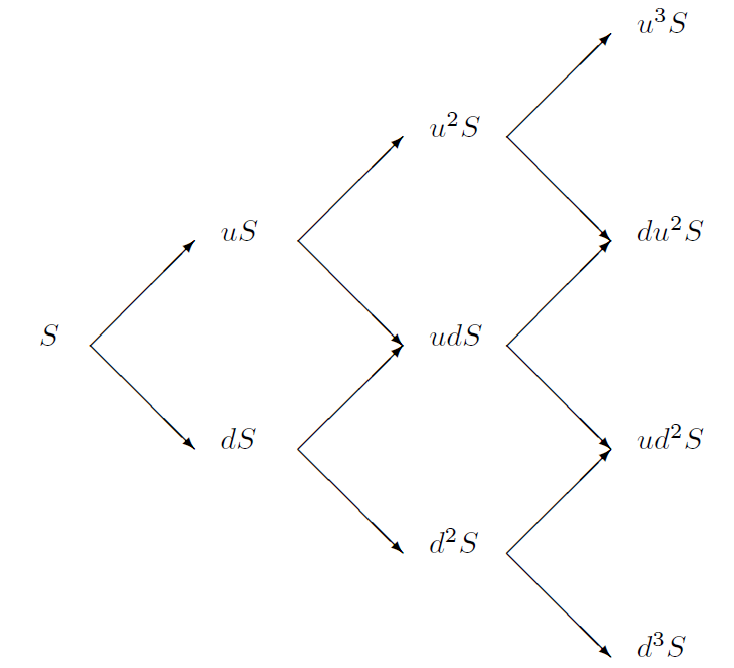
\includegraphics{docs/images/fig1.png}

A tree constructed like this is recombining in \index{recombining tree}
the sense that the stock price after an up-down sequence is the same as
after a down-up sequence. This is very important for reducing the
computation time. For example, the number of nodes at the final date is
\(N+1\) in a recombining tree, where \(N\) is the number of periods, but
it is \(2^N\) for a non-recombining (sometimes called bushy) tree.
Hence, the computation time will increase linearly with \(N\) for a
recombining tree but exponentially with \(N\) for a non-recombining
tree. Unfortunately, this computational savings is generally not
possible for path-dependent options, because the number of distinct
paths through a tree (whether recombining or not) is again \(2^N\).

The value of a European derivative is of course the discounted
expectation of its value at maturity, discounting at the risk-free rate
and taking the expectation under the risk-neutral measure. The binomial
tree allows us to approximate the expectation very easily. We simply sum
over the nodes of the tree at the option maturity and weight each node
by its binomial probability. In an \(N\)-period model, the probability
of the top node is \(p^N\), since the stock must go up each time to
reach the top node. There are \(N\) paths reaching the second node from
the top (since the period of the single down move could be any one of
the \(N\) periods) and each such path has probability \(p^{N-1}(1-p)\);
therefore, the probability of reaching the second node from the top is
\(Np^{N-1}(1-p)\). More generally, the probability of going up \(i\)
times and down \(N-i\) times is
\[\frac{N!}{i!(N-i)!}p^i(1-p)^{N-i}\; ,\] where as usual \(x!\) denotes
\(x\) factorial. Therefore, the expectation, for a European call option,
is the following sum over the \(N+1\) nodes at date \(N\) (starting with
\(i=0\) up moves and ending with \(i=N\) up moves):
\begin{equation}\phantomsection\label{eq-binomialsum}{
\sum_{i=0}^N \frac{N!}{i!(N-i)!}p^i(1-p)^{N-i}\max(u^id^{N-i}S-K,0)\;.
}\end{equation}

Multiplying the expectation by \(\mathrm{e}^{-rT}\) yields the option
value.

It is worthwhile to emphasize the close connection between this method
and the Monte-Carlo method discussed in the previous section. In the
Monte-Carlo method for valuing a European call option, we generate \(M\)
random values for \(S(T)\) and estimate the expectation
\(E^R[\max(0,S(T)-K)]\) by averaging the \(M\) values. This amounts to
approximating the distribution of \(S(T)\) by an \(M\)--point
distribution, each point being assigned equal probability. In the
binomial method, we choose a particular set of points for \(S(T)\) and
assign the probabilities specified above in order to approximate the
distribution of \(S(T)\). Both the Monte-Carlo and the binomial
approximations are known to converge to the continuous-time distribution
of \(S(T)\) as the number of points increases. However, by specifically
choosing the points and their probabilities, the binomial method allows
us to use a much smaller number of points to obtain the same accuracy;
i.e., for a given desired accuracy, we can use many fewer periods \(N\)
in the binomial model than we would need simulations \(M\) in the
Monte-Carlo method. Thus, the binomial method will be much faster.
Furthermore, as we will discuss in the next section, the binomial method
is much better for pricing American options. On the other hand, as
mentioned in the previous section, to value a path-dependent option in
an \(N\)--period binomial tree would require the analysis of \(2^N\)
separate paths, so Monte Carlo may be faster for path-dependent options.
Finally, as we will discuss in Section~\ref{sec-s_curse}, Monte Carlo
may be faster for options on multiple assets.

There is an important alternative method for calculating the sum
Equation~\ref{eq-binomialsum}, which is usually called backward
induction. \index{backward induction} We will describe it here and
implement it in the next section to value American options. We begin at
the last date, where there are \(N+1\) nodes. We calculate the option
value at each of these nodes, storing the value at the bottom node as
\(C(0)\), the value at the next node up as \(C(1)\), etc. This is
illustrated in the diagram on the next page. Then we step back to the
penultimate date. At each node at this date, we calculate the option
value as the discounted expectation of its value at the last date. From
each node, there are two nodes that can be reached at the next date,
corresponding to a down move or an up move. So, the option value is
calculated as \begin{equation}\phantomsection\label{eq-binomial001}{
C = \mathrm{e}^{-r\Delta t}p\,C_{\text{up}} + \mathrm{e}^{-r\Delta t}(1-p)C_{\text{down}}\;.
}\end{equation}

In terms of the vector notation shown in the figure below, the down move
from node \(i\) is also node \(i\) and the up move is \(i+1\). So, we
write over the elements of the \(C\) vector as
\begin{equation}\phantomsection\label{eq-binomial002}{
C(i) = \mathrm{e}^{-r\Delta t}p\,C(i+1) + \mathrm{e}^{-r\Delta t}(1-p)C(i)\;.
}\end{equation}

Discounting back through the tree like this, we reach date 0 and return
the option value as \(C(0)\). The virtue of this procedure is that it
calculates a value for the option at each node in the tree, the value
being the discounted expectation of the subsequent values attained by
the option. This approach is essential for assessing the value of early
exercise.

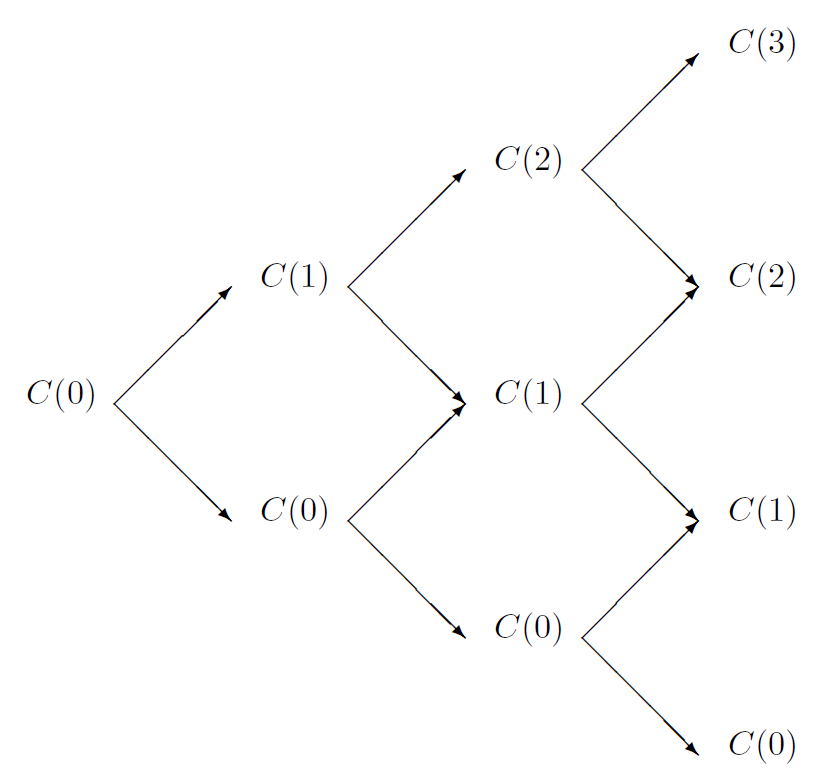
\includegraphics{docs/images/fig2.png}

\section{Binomial Parameters}\label{sec-s_binomialparameters}

Several different ways have been proposed for matching the binomial
model to the continuous-time model. Consider an \(N\)--period binomial
model for a time period of \(T\) years. This means that the length of
each period is \(\Delta t = T/N\). In the continuous-time model, over a
discrete time period \(\Delta t\), we have
\[\Delta \log S =\mathrm{n}u\,\Delta t + \sigma\,\Delta B\; ,\] where
\(\mathrm{n}u = r-q-\sigma^2/2\) and \(B\) is a Brownian motion under
the risk-neutral measure. The mean and variance, under the risk-neutral
measure, of \(\Delta \log S\) in the continuous-time model are
\begin{align*}
E^R[\Delta \log S] &= \mathrm{n}u\,\Delta t\; ,\\
\mathrm{var}^R[\Delta \log S]&=\sigma^2\Delta t\; ,
\end{align*} so \begin{align*}
\frac{E^R[\Delta \log S]}{\Delta t} &= \mathrm{n}u\; ,\\
\frac{\mathrm{var}^R[\Delta \log S]}{\Delta t}&=\sigma^2\;.
\end{align*} In the binomial model, we have \begin{align*}
\frac{E^R\big[\Delta \log S\big]}{\Delta t} &=\frac{p\,\log u+(1-p)\log d}{\Delta t}\; ,\\
\frac{\mathrm{var}^R\big[\Delta \log S\big] }{\Delta t}&=\frac{p\,(1-p)(\log u-\log d)^2}{\Delta t}\;.
\end{align*} In order for the binomial model to converge in the
appropriate sense to the continuous-time model as the number of periods
\(N \rightarrow \infty\) keeping the total amount of time \(T\) fixed
(equivalently, as \(\Delta t \rightarrow 0\)), it is sufficient that
\begin{align*}
\frac{p\log u+(1-p)\log d}{\Delta t} &\rightarrow \mathrm{n}u\; ,\\
\frac{p\,(1-p)(\log u-\log d)^2}{\Delta t} &\rightarrow \sigma^2\;.
\end{align*}

The most popular model is probably that proposed by Cox, Ross and
Rubinstein (Cox, Ross, and Rubinstein 1979),
\index{Cox-Ross-Rubinstein model} who set \(d=1/u\) and

\begin{equation}\phantomsection\label{eq-crru}{
u = \mathrm{e}^{\sigma\sqrt{\Delta t}}\;,
}\end{equation}

\begin{equation}\phantomsection\label{eq-crrp}{
p = \frac{\mathrm{e}^{(r-q)\Delta t}-d}{u-d}\;.
}\end{equation}

Another well-known model is that of Jarrow and Rudd (Jarrow and Rudd
1983), \index{Jarrow-Rudd model} who take \(p=1/2\) and

\begin{equation}\phantomsection\label{eq-jru}{
u = \exp\left(\left((r-q-\frac{1}{2}\sigma^2\right)\Delta t + \sigma\sqrt{\Delta t}\right)\;,
}\end{equation}

\begin{equation}\phantomsection\label{eq-jrd}{
d = \exp\left(\left((r-q-\frac{1}{2}\sigma^2\right)\Delta t - \sigma\sqrt{\Delta t}\right)\;.
}\end{equation}

Yet another method is proposed by Leisen and Reimer (Leisen and Reimer
1996), \index{Leisen-Reimer model} and Jackson and Staunton (Jackson and
Staunton 2001) show that it is more efficient for approximating the
Black-Scholes value of a European option than are the
Cox-Ross-Rubinstein and Jarrow-Rudd trees.

For illustration, the Cox-Ross-Rubinstein tree will be implemented
below.

\subsection{Binomial Valuation of European
Options}\label{binomial-valuation-of-european-options}

The binomial model for path-independent European options can be
implemented as follows. We will use the Cox-Ross-Rubinstein parameters.
We first define the binomial parameters and some useful constants,
denoting the probability \(p\,\) of an up move as \(pu\) and the
probability \(1-p\) of a down move as \(pd\). The routine below uses the
combinatoric function comb(N,i) to compute the term
\(\frac{N !}{i! (N-i)!}\).

\begin{Shaded}
\begin{Highlighting}[]
\ImportTok{import}\NormalTok{ numpy }\ImportTok{as}\NormalTok{ np}
\ImportTok{from}\NormalTok{ scipy.special }\ImportTok{import}\NormalTok{ comb}
\CommentTok{\# Binomial Model for European Option}

\NormalTok{r }\OperatorTok{=} \FloatTok{.1} \CommentTok{\# interest rate}
\NormalTok{sig }\OperatorTok{=} \FloatTok{.2} \CommentTok{\# volatility}
\NormalTok{T }\OperatorTok{=} \FloatTok{.5} \CommentTok{\# Expiration}
\NormalTok{div }\OperatorTok{=} \FloatTok{0.0} \CommentTok{\# Dividend}
\NormalTok{S0 }\OperatorTok{=} \DecValTok{42} \CommentTok{\# initial stock price}
\NormalTok{K }\OperatorTok{=} \DecValTok{40} \CommentTok{\# strike price}
\NormalTok{times }\OperatorTok{=}\DecValTok{100} \CommentTok{\# Number of steps}
\NormalTok{dt }\OperatorTok{=}\NormalTok{ T}\OperatorTok{/}\NormalTok{times}
\NormalTok{delt }\OperatorTok{=}\NormalTok{ np.exp(}\OperatorTok{{-}}\NormalTok{div}\OperatorTok{*}\NormalTok{dt)}
\NormalTok{a }\OperatorTok{=}\NormalTok{ np.exp(r}\OperatorTok{*}\NormalTok{dt)}\OperatorTok{*}\NormalTok{delt}
\NormalTok{u }\OperatorTok{=}\NormalTok{ np.exp(sig}\OperatorTok{*}\NormalTok{np.sqrt(dt))}
\NormalTok{d }\OperatorTok{=} \DecValTok{1}\OperatorTok{/}\NormalTok{u}
\NormalTok{pu  }\OperatorTok{=}\NormalTok{ (a}\OperatorTok{{-}}\NormalTok{d)}\OperatorTok{/}\NormalTok{(u}\OperatorTok{{-}}\NormalTok{d)}
\NormalTok{pd }\OperatorTok{=} \DecValTok{1}\OperatorTok{{-}}\NormalTok{pu}
\NormalTok{vec }\OperatorTok{=}\NormalTok{ np.arange(times }\OperatorTok{+} \DecValTok{1}\NormalTok{)}
\NormalTok{vec1 }\OperatorTok{=}\NormalTok{ np.array([}\DecValTok{1}\NormalTok{] }\OperatorTok{*}\NormalTok{ (times }\OperatorTok{+} \DecValTok{1}\NormalTok{))}
\NormalTok{S }\OperatorTok{=}\NormalTok{ np.array([}\DecValTok{0}\NormalTok{] }\OperatorTok{*}\NormalTok{ (times }\OperatorTok{+} \DecValTok{1}\NormalTok{))}
\NormalTok{S }\OperatorTok{=}\NormalTok{ S0}\OperatorTok{*}\NormalTok{u}\OperatorTok{**}\NormalTok{(}\DecValTok{2}\OperatorTok{*}\NormalTok{vec}\OperatorTok{{-}}\NormalTok{times}\OperatorTok{*}\NormalTok{vec1)}
\NormalTok{C }\OperatorTok{=}\NormalTok{  np.maximum(S}\OperatorTok{{-}}\NormalTok{K}\OperatorTok{*}\NormalTok{vec1,}\DecValTok{0}\OperatorTok{*}\NormalTok{vec1)}
\NormalTok{CC }\OperatorTok{=}\NormalTok{  comb((times)}\OperatorTok{*}\NormalTok{vec1,(times)}\OperatorTok{*}\NormalTok{vec1}\OperatorTok{{-}}\NormalTok{vec)}\OperatorTok{*}\NormalTok{pu}\OperatorTok{**}\NormalTok{(vec)}\OperatorTok{*}\NormalTok{pd}\OperatorTok{**}\NormalTok{(times}\OperatorTok{*}\NormalTok{vec1}\OperatorTok{{-}}\NormalTok{vec)}\OperatorTok{*}\NormalTok{C}
\NormalTok{Call }\OperatorTok{=} \BuiltInTok{sum}\NormalTok{(CC)}\OperatorTok{*}\NormalTok{np.exp(}\OperatorTok{{-}}\NormalTok{r}\OperatorTok{*}\NormalTok{T)}
\BuiltInTok{print}\NormalTok{(}\StringTok{\textquotesingle{}The Value of the European Call is=\textquotesingle{}}\NormalTok{,Call)}
\end{Highlighting}
\end{Shaded}

\begin{verbatim}
The Value of the European Call is= 4.761818357763364
\end{verbatim}

The Black Scholes value is shown below.

\begin{Shaded}
\begin{Highlighting}[]
\ImportTok{from}\NormalTok{ scipy }\ImportTok{import}\NormalTok{ stats}
\ImportTok{import}\NormalTok{ numpy }\ImportTok{as}\NormalTok{ np}
\ImportTok{from}\NormalTok{ scipy.optimize }\ImportTok{import}\NormalTok{ minimize, minimize\_scalar}

\KeywordTok{def}\NormalTok{ blackscholes(S0, K, r, q, sig, T, call }\OperatorTok{=} \VariableTok{True}\NormalTok{):}
    \CommentTok{\textquotesingle{}\textquotesingle{}\textquotesingle{}Calculate option price using B{-}S formula.}

\CommentTok{    Args:}
\CommentTok{        S0 (num): initial price of underlying asset.}
\CommentTok{        K (num): strick price.}
\CommentTok{        sig (num): Black{-}Scholes volatility.}
\CommentTok{        T (num): maturity.}
\CommentTok{        call (bool): True returns call price, False returns put price.}

\CommentTok{    Returns:}
\CommentTok{        num}
\CommentTok{    \textquotesingle{}\textquotesingle{}\textquotesingle{}}
\NormalTok{    d1 }\OperatorTok{=}\NormalTok{ (np.log(S0}\OperatorTok{/}\NormalTok{K) }\OperatorTok{+}\NormalTok{ (r }\OperatorTok{{-}}\NormalTok{q }\OperatorTok{+}\NormalTok{ sig}\OperatorTok{**}\DecValTok{2}\OperatorTok{/}\DecValTok{2}\NormalTok{) }\OperatorTok{*}\NormalTok{ T)}\OperatorTok{/}\NormalTok{(sig}\OperatorTok{*}\NormalTok{np.sqrt(T))}
\NormalTok{    d2 }\OperatorTok{=}\NormalTok{ d1 }\OperatorTok{{-}}\NormalTok{ sig}\OperatorTok{*}\NormalTok{np.sqrt(T)}
\CommentTok{\#     norm = sp.stats.norm}
\NormalTok{    norm }\OperatorTok{=}\NormalTok{ stats.norm}
    \ControlFlowTok{if}\NormalTok{ call:}
        \ControlFlowTok{return}\NormalTok{ np.exp(}\OperatorTok{{-}}\NormalTok{q}\OperatorTok{*}\NormalTok{T)}\OperatorTok{*}\NormalTok{S0 }\OperatorTok{*}\NormalTok{ norm.cdf(d1,}\DecValTok{0}\NormalTok{,}\DecValTok{1}\NormalTok{) }\OperatorTok{{-}}\NormalTok{ K }\OperatorTok{*}\NormalTok{ np.exp(}\OperatorTok{{-}}\NormalTok{r }\OperatorTok{*}\NormalTok{ T) }\OperatorTok{*}\NormalTok{ norm.cdf(d2,}\DecValTok{0}\NormalTok{, }\DecValTok{1}\NormalTok{)}
    \ControlFlowTok{else}\NormalTok{:}
        \ControlFlowTok{return} \OperatorTok{{-}}\NormalTok{np.exp(}\OperatorTok{{-}}\NormalTok{q}\OperatorTok{*}\NormalTok{T)}\OperatorTok{*}\NormalTok{S0 }\OperatorTok{*}\NormalTok{ norm.cdf(}\OperatorTok{{-}}\NormalTok{d1,}\DecValTok{0}\NormalTok{,}\DecValTok{1}\NormalTok{) }\OperatorTok{+}\NormalTok{K }\OperatorTok{*}\NormalTok{ np.exp(}\OperatorTok{{-}}\NormalTok{r }\OperatorTok{*}\NormalTok{ T) }\OperatorTok{*}\NormalTok{ norm.cdf(}\OperatorTok{{-}}\NormalTok{d2,}\DecValTok{0}\NormalTok{, }\DecValTok{1}\NormalTok{)}

\NormalTok{truebsc }\OperatorTok{=}\NormalTok{ blackscholes(S0,K,r, div, sig,T)}
\BuiltInTok{print}\NormalTok{(}\StringTok{\textquotesingle{}The exact Black Scholes Price is=\textquotesingle{}}\NormalTok{, truebsc)}
\end{Highlighting}
\end{Shaded}

\begin{verbatim}
The exact Black Scholes Price is= 4.759422392871532
\end{verbatim}

An alternative way to calculate te value of the call is to use a loop.
This takes longer to run but is perhaps easier to understand.

\begin{Shaded}
\begin{Highlighting}[]
\ControlFlowTok{for}\NormalTok{ i }\KeywordTok{in} \BuiltInTok{range}\NormalTok{(times}\OperatorTok{+}\DecValTok{1}\NormalTok{):}
\NormalTok{    S[i] }\OperatorTok{=}\NormalTok{ S0}\OperatorTok{*}\NormalTok{u }\OperatorTok{**}\NormalTok{ (}\DecValTok{2}\OperatorTok{*}\NormalTok{i}\OperatorTok{{-}}\NormalTok{times)}
\NormalTok{    C[i] }\OperatorTok{=}  \BuiltInTok{max}\NormalTok{(S[i]}\OperatorTok{{-}}\NormalTok{K,}\DecValTok{0}\NormalTok{)}

\NormalTok{    CC[i] }\OperatorTok{=}\NormalTok{  comb((times),(i))}\OperatorTok{*}\NormalTok{pu }\OperatorTok{**}\NormalTok{ (i)}\OperatorTok{*}\NormalTok{pd }\OperatorTok{**}\NormalTok{ (times}\OperatorTok{{-}}\NormalTok{i)}\OperatorTok{*}\NormalTok{C[i]}



\NormalTok{Call }\OperatorTok{=} \BuiltInTok{sum}\NormalTok{(CC)}\OperatorTok{*}\NormalTok{np.exp(}\OperatorTok{{-}}\NormalTok{r}\OperatorTok{*}\NormalTok{T)}
\BuiltInTok{print}\NormalTok{(}\StringTok{\textquotesingle{}The Value of the European Call is=\textquotesingle{}}\NormalTok{,Call)}
\end{Highlighting}
\end{Shaded}

\begin{verbatim}
The Value of the European Call is= 4.761818357763364
\end{verbatim}

\section{Binomial Models for American
Options}\label{binomial-models-for-american-options}

Early exercise \index{early exercise} features are very simple to handle
in a binomial framework. One only has to use the backward induction
approach and check the optimality of early exercise at each node.
Exercise is optimal when the intrinsic value of the option exceeds the
discounted expected value of the option contingent on not exercising.
When we back up in the tree, we check whether exercise is optimal, and,
when it is, we replace the discounted expected value with the intrinsic
value.

Early exercise is more important for puts than for calls (as discussed
in Section~\ref{sec-s_fundamentalconcepts}, an American call on a
non-dividend-paying stock should not be exercised early) so we will
change our symbol for the option value from \(C\) to \(P\). For a put
option, we would calculate the value at each node at the end of the tree
as described in the previous section:
\begin{equation}\phantomsection\label{eq-binomial003}{
P(i) = \max\left(0,K-u^{i}d^{N-i}S\right)\;,
}\end{equation}

for \(i=0,\ldots,N\). For a European put, we would also back up in the
tree in accord with Equation~\ref{eq-binomial002}:
\begin{equation}\phantomsection\label{eq-binomial004}{
P(i) = \mathrm{e}^{-r\Delta t}p\,P(i+1) + \mathrm{e}^{-r\Delta t}(1-p)P(i)\;.
}\end{equation}

To accommodate early exercise, we simply need to assign to \(P(i)\) the
larger of this value and the value of early exercise. At node \(i\) at
date \(n\) the stock price is \(u^{i}d^{n-i}S\) and the intrinsic value
of a put option is \(\max(0,K-u^{i}d^{n-i}S)\). Therefore we replace
Equation~\ref{eq-binomial004} with
\begin{equation}\phantomsection\label{eq-binomial005}{
P(i) = \max\big(K-u^{i}d^{n-i}S, \;\mathrm{e}^{-r\Delta t}p\,P(i+1) + \mathrm{e}^{-r\Delta t}(1-p)P(i)\big)\;.
}\end{equation}

This will be explained in more detail in \textbf{?@sec-s\_introcompvba}.

\subsection{Binomial Valuation of American
Options}\label{binomial-valuation-of-american-options}

We will consider an American put. It may also be optimal to exercise an
American call early, if there is a positive dividend yield, and the same
procedure can be used for American calls. We begin as in the previous
subsection by defining the binomial parameters, some useful constants,
and the stock price at the last date. We also record the value of the
lowest stock price where we exercise at the last date \(ex[n]\).

\begin{Shaded}
\begin{Highlighting}[]
\ImportTok{import}\NormalTok{ numpy }\ImportTok{as}\NormalTok{ np}
\ImportTok{import}\NormalTok{ matplotlib.pyplot }\ImportTok{as}\NormalTok{ plt}
\ImportTok{import}\NormalTok{ time}
\ImportTok{from}\NormalTok{ math }\ImportTok{import} \BuiltInTok{pow}\NormalTok{, exp, sqrt}
\CommentTok{\# parameters}
\CommentTok{\# number of steps}
\NormalTok{n }\OperatorTok{=} \DecValTok{100}
\CommentTok{\# interest rate}
\NormalTok{r }\OperatorTok{=} \FloatTok{.1}
\CommentTok{\# true drift}
\NormalTok{mu }\OperatorTok{=} \FloatTok{.15}
\CommentTok{\# volatility}
\NormalTok{sig }\OperatorTok{=} \FloatTok{.2}
\CommentTok{\# Initial Stock Price}
\NormalTok{S0 }\OperatorTok{=} \DecValTok{42}
\CommentTok{\# Strike Price}
\NormalTok{K }\OperatorTok{=} \DecValTok{42}
\CommentTok{\# Maturity}
\NormalTok{T }\OperatorTok{=} \FloatTok{0.5}
\CommentTok{\# dividend yield}
\NormalTok{y }\OperatorTok{=} \DecValTok{0}

\CommentTok{\# calculate parameters for binomial model}
\NormalTok{dt }\OperatorTok{=}\NormalTok{ T}\OperatorTok{/}\NormalTok{n}
\NormalTok{delt }\OperatorTok{=}\NormalTok{ np.exp(}\OperatorTok{{-}}\NormalTok{y}\OperatorTok{*}\NormalTok{dt)}
\NormalTok{a }\OperatorTok{=}\NormalTok{ np.exp(r}\OperatorTok{*}\NormalTok{dt) }\OperatorTok{*}\NormalTok{ delt}
\NormalTok{u }\OperatorTok{=}\NormalTok{ np.exp(sig}\OperatorTok{*}\NormalTok{np.sqrt(dt))}
\NormalTok{d }\OperatorTok{=} \DecValTok{1}\OperatorTok{/}\NormalTok{u}
\NormalTok{pu }\OperatorTok{=}\NormalTok{ (a}\OperatorTok{{-}}\NormalTok{d)}\OperatorTok{/}\NormalTok{(u}\OperatorTok{{-}}\NormalTok{d)}
\NormalTok{pd }\OperatorTok{=} \DecValTok{1}\OperatorTok{{-}}\NormalTok{pu}
\CommentTok{\# Build vector of ending values}
\CommentTok{\# and prices for which put is exercised}
\NormalTok{ex }\OperatorTok{=}\NormalTok{ np.zeros(n}\OperatorTok{+}\DecValTok{1}\NormalTok{)}
\NormalTok{S }\OperatorTok{=}\NormalTok{ np.zeros(n}\OperatorTok{+}\DecValTok{1}\NormalTok{)}
\NormalTok{AP }\OperatorTok{=}\NormalTok{ np.zeros(n}\OperatorTok{+}\DecValTok{1}\NormalTok{)}

\ControlFlowTok{for}\NormalTok{ j }\KeywordTok{in} \BuiltInTok{range}\NormalTok{(n}\OperatorTok{+}\DecValTok{1}\NormalTok{):}
\NormalTok{    S[j] }\OperatorTok{=}\NormalTok{ S0}\OperatorTok{*}\NormalTok{u}\OperatorTok{**}\NormalTok{(}\DecValTok{2}\OperatorTok{*}\NormalTok{j}\OperatorTok{{-}}\NormalTok{n)}
\NormalTok{    AP[j] }\OperatorTok{=} \BuiltInTok{max}\NormalTok{(K}\OperatorTok{{-}}\NormalTok{S[j],}\DecValTok{0}\NormalTok{)}
    \ControlFlowTok{if}\NormalTok{ AP[j]}\OperatorTok{\textgreater{}}\DecValTok{0}\NormalTok{:}
\NormalTok{        ex[n] }\OperatorTok{=}\NormalTok{ S[j]}
\end{Highlighting}
\end{Shaded}

Now we do the backward induction. Note that a period is the time period
between successive dates. In a one-period model, there are two dates
(the beginning and end) and in general there are \(N+1\) dates in an
\(N\)--period model. We index the dates as \(i=0,\ldots,N\). At each
date we start by defining the stock price at the bottom node. At date
\(i\) there have been \(i\) past periods, so the bottom node corresponds
to \(i\) down moves. The put value at each node is computed as the
larger of the discounted expected value and the value of immediate
exercise (the intrinsic value). Having already dealt with the bottom
node (\(j=0\)) we loop over the nodes \(j=1,\ldots,i\) at each date
\(i\), increasing the stock price by a factor of \(u^2\) each time. When
we have backed up to date 0, we return the put value \(AP(0)\), the
value at the bottom node, which is the only node at
date\textasciitilde0.

\begin{Shaded}
\begin{Highlighting}[]
\ControlFlowTok{for}\NormalTok{ i }\KeywordTok{in} \BuiltInTok{range}\NormalTok{(n):}
\NormalTok{    S }\OperatorTok{=}\NormalTok{ np.zeros(n}\OperatorTok{{-}}\NormalTok{i)}
\NormalTok{    P }\OperatorTok{=}\NormalTok{ np.zeros(n}\OperatorTok{{-}}\NormalTok{i)}
\NormalTok{    PP }\OperatorTok{=}\NormalTok{ np.zeros(n}\OperatorTok{{-}}\NormalTok{i)}
    \ControlFlowTok{for}\NormalTok{ j }\KeywordTok{in} \BuiltInTok{range}\NormalTok{(n}\OperatorTok{{-}}\NormalTok{i):}
\NormalTok{        S[j] }\OperatorTok{=}\NormalTok{ S0}\OperatorTok{*}\NormalTok{u}\OperatorTok{**}\NormalTok{(}\DecValTok{2}\OperatorTok{*}\NormalTok{j}\OperatorTok{{-}}\NormalTok{(n}\OperatorTok{{-}}\NormalTok{i}\OperatorTok{{-}}\DecValTok{1}\NormalTok{))}
        \CommentTok{\#}
        \CommentTok{\# P calculates the value of early exercise}
\NormalTok{        P[j] }\OperatorTok{=} \BuiltInTok{max}\NormalTok{(K}\OperatorTok{{-}}\NormalTok{S[j],}\DecValTok{0}\NormalTok{)}
        \CommentTok{\#}
        \CommentTok{\# PP calculates value of waiting using payoffs}
        \CommentTok{\# from next period}
\NormalTok{        PP[j] }\OperatorTok{=}\NormalTok{ (pu}\OperatorTok{*}\NormalTok{AP[j}\OperatorTok{+}\DecValTok{1}\NormalTok{] }\OperatorTok{+}\NormalTok{ pd}\OperatorTok{*}\NormalTok{AP[j])}\OperatorTok{/}\NormalTok{a}
        \CommentTok{\#}
        \CommentTok{\# AP is the max of ealry exercise and waiting}
\NormalTok{        AP[j] }\OperatorTok{=} \BuiltInTok{max}\NormalTok{(P[j],PP[j])}
        \CommentTok{\#}
        \CommentTok{\# ex is price where early exercise is optimal}
        \ControlFlowTok{if}\NormalTok{ P[j] }\OperatorTok{\textgreater{}}\NormalTok{ PP[j]:}
\NormalTok{            ex[n}\OperatorTok{{-}}\NormalTok{i] }\OperatorTok{=}\NormalTok{ S[j]}
        \ControlFlowTok{if}\NormalTok{ ex[n}\OperatorTok{{-}}\NormalTok{i]}\OperatorTok{==}\DecValTok{0}\NormalTok{:}
\NormalTok{           ex[n}\OperatorTok{{-}}\NormalTok{i]}\OperatorTok{=}\NormalTok{np.nan}
               

\BuiltInTok{print}\NormalTok{(}\StringTok{\textquotesingle{}The value of the American Put is=\textquotesingle{}}\NormalTok{,AP[}\DecValTok{0}\NormalTok{])}
\NormalTok{plt.figure(figsize}\OperatorTok{=}\NormalTok{(}\DecValTok{9}\NormalTok{,}\DecValTok{6}\NormalTok{))}
\NormalTok{plt.plot(dt}\OperatorTok{*}\NormalTok{np.arange(n}\OperatorTok{+}\DecValTok{1}\NormalTok{),ex)}
\end{Highlighting}
\end{Shaded}

\begin{verbatim}
The value of the American Put is= 1.643396346909605
\end{verbatim}

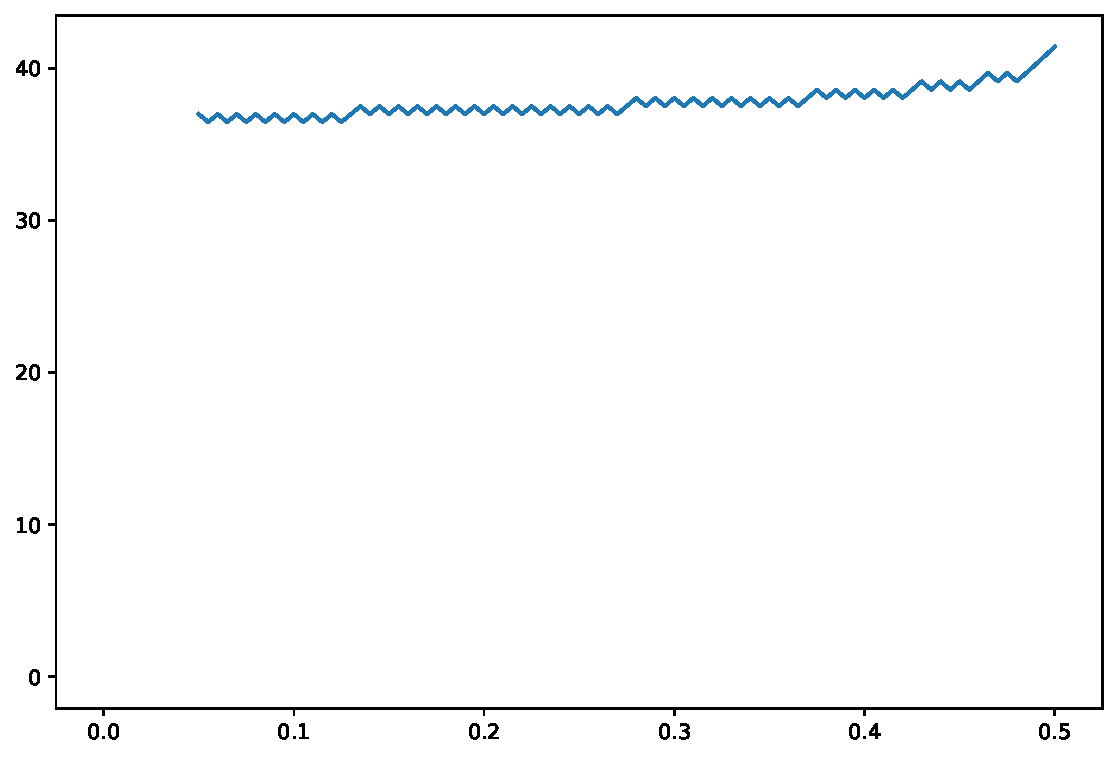
\includegraphics{Chapter6_files/figure-pdf/cell-12-output-2.pdf}

The above code runs slowly due to the loops and looping is inefficient
in Python. Below we provide a code which generatee the same answer
except one of the loops is replaced by vector calculations. The program
creates the stock price for each time in a vector and uses vector
comparisons to calcualte the maximum of the early exercise and waiting.
To understand the code, it is probably a good idea to print out vec1 and
vec to see how the exponents are calulated at each node. This procedure
is necessary to speed up the execution since loops are inefficient in
Python.

\begin{Shaded}
\begin{Highlighting}[]
\ImportTok{import}\NormalTok{ numpy }\ImportTok{as}\NormalTok{ np}
\ImportTok{import}\NormalTok{ matplotlib.pyplot }\ImportTok{as}\NormalTok{ plt}
\ImportTok{import}\NormalTok{ time}
\ImportTok{from}\NormalTok{ math }\ImportTok{import} \BuiltInTok{pow}\NormalTok{, exp, sqrt}
\CommentTok{\# parameters}
\CommentTok{\# number of steps}
\NormalTok{n }\OperatorTok{=} \DecValTok{100}
\CommentTok{\# interest rate}
\NormalTok{r }\OperatorTok{=} \FloatTok{.1}
\CommentTok{\# true drift}
\NormalTok{mu }\OperatorTok{=} \FloatTok{.15}
\CommentTok{\# volatility}
\NormalTok{sig }\OperatorTok{=} \FloatTok{.2}
\CommentTok{\# Initial Stock Price}
\NormalTok{S0 }\OperatorTok{=} \DecValTok{42}
\CommentTok{\# Strike Price}
\NormalTok{K }\OperatorTok{=} \DecValTok{42}
\CommentTok{\# Maturity}
\NormalTok{T }\OperatorTok{=} \FloatTok{0.5}
\CommentTok{\# dividend yield}
\NormalTok{y }\OperatorTok{=} \DecValTok{0}

\NormalTok{dt }\OperatorTok{=}\NormalTok{ T}\OperatorTok{/}\NormalTok{n}
\NormalTok{delt }\OperatorTok{=}\NormalTok{ np.exp(}\OperatorTok{{-}}\NormalTok{y}\OperatorTok{*}\NormalTok{dt)}
\NormalTok{a }\OperatorTok{=}\NormalTok{ np.exp(r}\OperatorTok{*}\NormalTok{dt) }\OperatorTok{*}\NormalTok{ delt}
\NormalTok{u }\OperatorTok{=}\NormalTok{ np.exp(sig}\OperatorTok{*}\NormalTok{np.sqrt(dt))}
\NormalTok{d }\OperatorTok{=} \DecValTok{1}\OperatorTok{/}\NormalTok{u}
\NormalTok{pu }\OperatorTok{=}\NormalTok{ (a}\OperatorTok{{-}}\NormalTok{d)}\OperatorTok{/}\NormalTok{(u}\OperatorTok{{-}}\NormalTok{d)}
\NormalTok{pd }\OperatorTok{=} \DecValTok{1}\OperatorTok{{-}}\NormalTok{pu}
\CommentTok{\# Build vector of ending values}
\CommentTok{\# and prices for which put is exercised}
\NormalTok{vec }\OperatorTok{=}\NormalTok{ np.arange(n}\OperatorTok{+}\DecValTok{1}\NormalTok{)}
\NormalTok{vec1 }\OperatorTok{=}\NormalTok{ np.ones(n}\OperatorTok{+}\DecValTok{1}\NormalTok{)}

\NormalTok{S }\OperatorTok{=}\NormalTok{ S0 }\OperatorTok{*}\NormalTok{ u}\OperatorTok{**}\NormalTok{(}\DecValTok{2}\OperatorTok{*}\NormalTok{vec }\OperatorTok{{-}}\NormalTok{ n}\OperatorTok{*}\NormalTok{vec1)}

\NormalTok{AP }\OperatorTok{=}\NormalTok{ np.maximum(K}\OperatorTok{{-}}\NormalTok{S,}\DecValTok{0}\NormalTok{)}
\CommentTok{\#print(AP)}
\NormalTok{ex }\OperatorTok{=}\NormalTok{ S[AP}\OperatorTok{\textgreater{}}\DecValTok{0}\NormalTok{]}
\NormalTok{eb }\OperatorTok{=}\NormalTok{ np.zeros(n}\OperatorTok{+}\DecValTok{1}\NormalTok{)}
\NormalTok{eb[n] }\OperatorTok{=}\NormalTok{ ex.}\BuiltInTok{max}\NormalTok{()}
\CommentTok{\# Backward recursion in the loop}
\ControlFlowTok{for}\NormalTok{ i }\KeywordTok{in} \BuiltInTok{range}\NormalTok{(n):}
\NormalTok{    vec }\OperatorTok{=}\NormalTok{ np.arange(n}\OperatorTok{{-}}\NormalTok{i)}
\NormalTok{    vec1 }\OperatorTok{=}\NormalTok{ np.ones(n}\OperatorTok{{-}}\NormalTok{i)}
    \CommentTok{\# Possible Stock prices at times{-}i period}
\NormalTok{    S }\OperatorTok{=}\NormalTok{ S0 }\OperatorTok{*}\NormalTok{ u}\OperatorTok{**}\NormalTok{(}\DecValTok{2}\OperatorTok{*}\NormalTok{vec}\OperatorTok{{-}}\NormalTok{(n}\OperatorTok{{-}}\NormalTok{i)}\OperatorTok{*}\NormalTok{vec1}\OperatorTok{+}\DecValTok{1}\NormalTok{)}
\CommentTok{\#     S = S0 * u**(2*vec{-}(n{-}i))}
    \CommentTok{\# P calculates the value of early exercise}
\NormalTok{    P }\OperatorTok{=}\NormalTok{ np.maximum(K}\OperatorTok{*}\NormalTok{vec1 }\OperatorTok{{-}}\NormalTok{ S, }\DecValTok{0}\NormalTok{)}
    \CommentTok{\# PP calculates value of waiting using payoffs from next period}
\NormalTok{    PP }\OperatorTok{=}\NormalTok{ (pu}\OperatorTok{*}\NormalTok{AP[}\DecValTok{1}\NormalTok{:(n}\OperatorTok{{-}}\NormalTok{i}\OperatorTok{+}\DecValTok{1}\NormalTok{)] }\OperatorTok{+}\NormalTok{ pd}\OperatorTok{*}\NormalTok{AP[}\DecValTok{0}\NormalTok{:(n}\OperatorTok{{-}}\NormalTok{i)])}\OperatorTok{/}\NormalTok{a}
    \CommentTok{\# AP is the max of ealry exercise and waiting}
\NormalTok{    AP }\OperatorTok{=}\NormalTok{ np.maximum(P,PP)}
    \CommentTok{\# ex is prices where early exercise is optimal}
\NormalTok{    ex }\OperatorTok{=}\NormalTok{ S[AP}\OperatorTok{{-}}\NormalTok{PP}\OperatorTok{\textgreater{}}\DecValTok{0}\NormalTok{]}
    \CommentTok{\# eb calculates the highest price}
    \CommentTok{\# where exercise is optimal to plot boundary}
    \ControlFlowTok{if}\NormalTok{ ex.shape[}\DecValTok{0}\NormalTok{]}\OperatorTok{\textgreater{}}\DecValTok{0}\NormalTok{:}
\NormalTok{        eb[n}\OperatorTok{{-}}\NormalTok{i] }\OperatorTok{=}\NormalTok{ ex.}\BuiltInTok{max}\NormalTok{()}
    \ControlFlowTok{else}\NormalTok{:}
\NormalTok{        eb[n}\OperatorTok{{-}}\NormalTok{i] }\OperatorTok{=}\NormalTok{ np.nan}

\BuiltInTok{print}\NormalTok{(}\StringTok{\textquotesingle{}The value of the American Put is=\textquotesingle{}}\NormalTok{,AP[}\DecValTok{0}\NormalTok{])        }
     \CommentTok{\# plot the exercise boundary}
\NormalTok{plt.figure(figsize}\OperatorTok{=}\NormalTok{(}\DecValTok{9}\NormalTok{,}\DecValTok{6}\NormalTok{))}
\NormalTok{plt.plot(dt}\OperatorTok{*}\NormalTok{np.arange(n}\OperatorTok{+}\DecValTok{1}\NormalTok{),eb)}
\end{Highlighting}
\end{Shaded}

\begin{verbatim}
The value of the American Put is= 1.643396346909605
\end{verbatim}

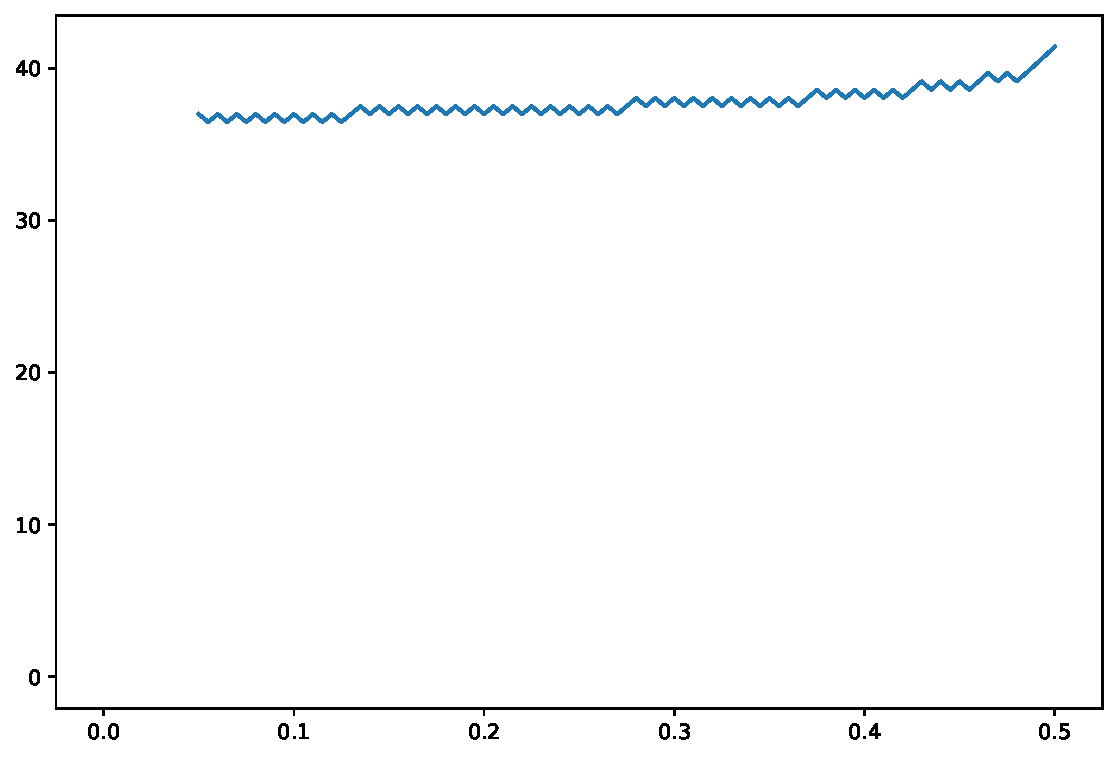
\includegraphics{Chapter6_files/figure-pdf/cell-13-output-2.pdf}

However, when we consider binomial models for multiple assets in
\textbf{?@sec-c\_montecarlo}, we will use the tree proposed by
Trigeorgis (Trigeorgis 1991), \index{Trigeorgis model} because it is the
simplest to explain in that context. Trigeorgis proposes choosing \(p\),
\(u\) and \(d\) so that the mean and variance of \(\Delta \log S\) in
the binomial model match those in the continuous-time model exactly.
This means that

\begin{align*}
\frac{p\log u+(1-p)\log d}{\Delta t} &= \mathrm{n}u\; ,\\
\frac{p(1-p)(\log u-\log d)^2}{\Delta t} &= \sigma^2\;.
\end{align*}

These are two equations in the three unknowns, leaving one degree of
freedom, so Trigeorgis takes \(d=1/u\), as do Cox, Ross and Rubinstein.
As we will show in the next section, taking \(d=1/u\) simplifies the
calculations of deltas and gammas. Solving these two equations
yields\^{}{[}Notice that if we were to drop the \((\Delta t)^2\) term in
Equation~\ref{eq-trig1} (which we could do because it becomes
increasingly negligible as \(\Delta t \rightarrow 0)\), then
Equation~\ref{eq-trig1} would be the same as Equation~\ref{eq-crru}. The
different choices of \(p\) in Equation~\ref{eq-crrp} and
Equation~\ref{eq-trig2} can be understood as follows. Equation
Equation~\ref{eq-crrp} implies that the expected stock price
\(pS_u + (1-p)S_d\) equals \(\mathrm{e}^{(r-q)\Delta t}S\), so we have
average growth at the rate \(r-q\) as in the continuous-time model. On
the other hand, Equation~\ref{eq-trig2} implies that the expected
\emph{log} stock price \(p \,\log S_u + (1-p) \log S_d\) equals
\(\log S + \mathrm{n}u \Delta t\), so the expected change in the
logarithm is \(\mathrm{n}u\Delta t\), also as in the continuous-time
model. Thus, both match the binomial model to the continuous-time model,
the Cox-Ross-Rubinstein method focusing on the expected return
(equivalently, the expected change in the price of the underlying) and
the Trigeorgis method focusing on the expected continuously-compounded
return (the expected change in the logarithm of the price).\}

\begin{equation}\phantomsection\label{eq-trig1}{
\log u=\sqrt{\sigma^2\Delta t + \mathrm{n}u^2(\Delta t)^2}\;,
}\end{equation}

\begin{equation}\phantomsection\label{eq-trig2}{
p = \frac{1}{2}+\frac{\mathrm{n}u\Delta t}{2\log u}\;.
}\end{equation}

\section{Binomial Greeks}\label{sec-s_binomial_greeks}

To estimate Greeks in any valuation model, one can run the valuation
program twice, for two different parameter values, and then estimate the
Greek as the difference in value divided by the difference in
parameters. For example, to estimate vega when the volatility of the
underlying is \(\sigma\), we could estimate the derivative value for a
volatility of \(0.99\sigma\) and for a volatility of \(1.01\sigma\).
Denoting the former derivative value by \(C_d\) and the latter by
\(C_u\), the vega can be estimated by
\[\frac{C_u-C_d}{1.01\sigma-0.99\sigma} = \frac{C_u-C_d}{0.02\sigma}\; .\]
We can in principle obtain a more precise estimate of the derivative by
making a smaller change in the parameter (e.g., using \(0.999\sigma\)
and \(1.001\sigma\)) but computer round-off errors limit how small a
parameter change one should take in practice.

To estimate the gamma when the price of the underlying is \(S\), we need
to estimate the derivative value at two other prices for the underlying,
which we will call \(S_u\) and \(S_d\), with \(S_u>S>S_d\). As just
explained, the estimate of the delta (which we continue to denote by
\(\delta\)) would be
\begin{equation}\phantomsection\label{eq-binomialdelta100}{
\delta = \frac{C_u-C_d}{S_u-S_d}\;,
}\end{equation}

where \(C_u\) denotes the derivative value when the underlying is equal
to \(S_u\) and \(C_d\) denotes the derivative value when the underlying
is equal to \(S_d\). Letting \(C\) denote the derivative value when the
underlying is equal to \(S\), two other obvious estimates of the delta
are
\[\delta_u = \frac{C_u-C}{S_u-S} \qquad \text{and} \qquad \delta_d = \frac{C-C_d}{S-S_d}\; .\]
The first of these should be understood as an estimate of the delta when
the price of the underlying is at the midpoint of \(S_u\) and \(S\), and
the second is an estimate of the delta when the price of the underlying
is at the midpoint of \(S_d\) and \(S\). The distance between these
midpoints is
\[\frac{S_u+S}{2} - \frac{S_d+S}{2} = \frac{S_u-S_d}{2}\; ,\] so we
obtain an estimate of \(\Gamma\) (the derivative of \(\delta\)) as
\begin{equation}\phantomsection\label{eq-binomialgamma100}{
\Gamma = \frac{\delta_u-\delta_d}{(S_u-S_d)/2}\;.
}\end{equation}

In a binomial model, it is possible to compute the most important
Greeks, delta and gamma, more efficiently than by simply running the
valuation program several times. Assume we have taken \(d=1/u\), so
after an up and a down move (or a down and an up move) the stock price
returns to its initial value \(S\). After fixing the length
\(\Delta t = T/N\) of each time period, we redefine \(N=N+2\). This
results in an \(N+2\) period tree covering a time period of length
\(T+2\Delta t\). Now consider the tree starting two periods from the
initial date. At the middle node shown below, the stock price is
\(udS=S\). Ignoring the top and bottom nodes and the branches that
follow them, the result of adding two periods is that the tree starting
from \(udS\) is an \(N\)--period tree for a time period of length \(T\).

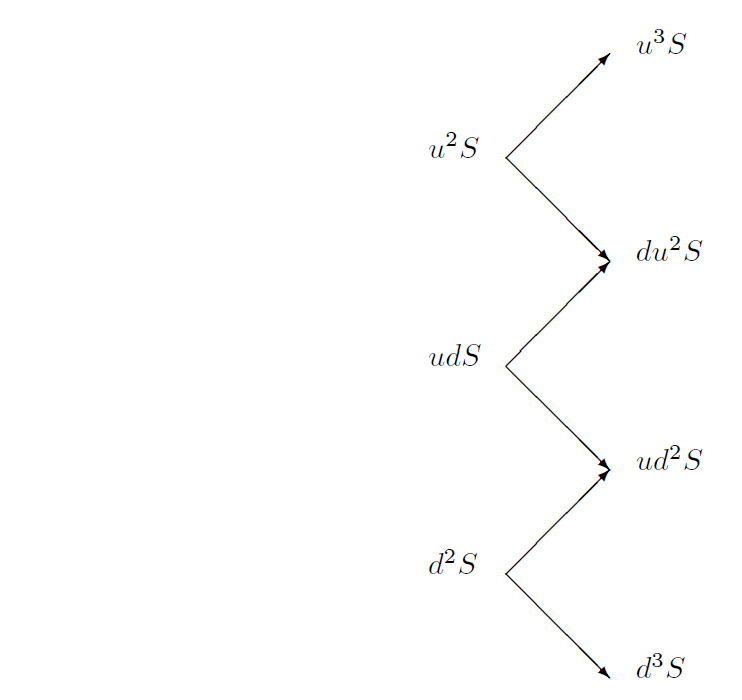
\includegraphics{docs/images/fig3.png}

Hence, the derivative price calculated at the middle node will be the
price we are trying to estimate. The derivative price at the top node
will be the value of a derivative of maturity \(T\) when the initial
price of the underlying is \(u^2S\). Similarly, the derivative price at
the bottom node will be the value of a derivative of maturity \(T\) when
the initial price of the underlying is \(d^2S\). Thus, when we back up
in the tree to this date, we will have all of the information we need to
return an estimate of the derivative value and to return estimates of
the delta and gamma, taking \(S_u=u^2S\) and \(S_d = d^2S\) in equations
Equation~\ref{eq-binomialdelta100} and
Equation~\ref{eq-binomialgamma100}. We are not interested in the tree to
the left of what is shown above.

\subsection{Trinomial Valuation of American
Options}\label{trinomial-valuation-of-american-options}

The trinomial model is a special case of an explicit finite difference
method for solving partial differnetial equations studied in
Chapter~\ref{sec-c_pde}; however, it requires no knowledge of partial
differential equations. It is similar to a binomial model in that it is
a tree. As the name suggests, the trinomial model has three branches up,
down, and middle. The middle branch eliminates the up down behavior and
can lead to smoother exercise boundaries. We will use the following
parameterization: at each node the stock price grows by a factor
\(u=e^{\sigma \sqrt{3 \Delta t}}\), stays the same, or declines by a
factor of \(d=1/u\). In this sense, it inherits some of the tractabilty
of the Cox, Ross, and Rubenstein model in the sense that the stock price
at all nodes can be expressed as the initial stock price times \(u\) to
a power. The probabilities are given by

\[
p_u = \frac{1}{6} + \sqrt{\frac{\Delta t}{12 \sigma^2}} \left(r - \frac{\sigma^2}{2}\right)~~~p_m =2/3~~p_d= \frac{1}{6} - \sqrt{\frac{\Delta t}{12 \sigma^2}} \left(r - \frac{\sigma^2}{2}\right)
\]

While there are many choices for the parameterization they are not
completely arbitrary. The probability \(p_m =2/3\) roughly corresponds
to plus or minus one standard devation of a normal distribution and the
up and down probabilities capture the tails. There are other
parameterizations which can work ust as well.

Conceptually, although there are three states and only two assets and
the market is incomplete, the model converges to the Black Scholes model
but there is no direct replication strategy. Nevertheless, we are
modelling the price in a risk neutral measure. More importantly it does
potentially give a better estimate of derivative prices.

\begin{Shaded}
\begin{Highlighting}[]
\ImportTok{import}\NormalTok{ numpy }\ImportTok{as}\NormalTok{ np}
\ImportTok{import}\NormalTok{ matplotlib.pyplot }\ImportTok{as}\NormalTok{ plt}
\ImportTok{import}\NormalTok{ time}
\ImportTok{from}\NormalTok{ math }\ImportTok{import} \BuiltInTok{pow}\NormalTok{, exp, sqrt}
\CommentTok{\# parameters}
\CommentTok{\# number of steps}
\NormalTok{n }\OperatorTok{=} \DecValTok{100}
\CommentTok{\# interest rate}
\NormalTok{r }\OperatorTok{=} \FloatTok{.1}
\CommentTok{\# volatility}
\NormalTok{sig }\OperatorTok{=} \FloatTok{.2}
\CommentTok{\# Initial Stock Price}
\NormalTok{S0 }\OperatorTok{=} \DecValTok{42}
\CommentTok{\# Strike Price}
\NormalTok{K }\OperatorTok{=} \DecValTok{42}
\CommentTok{\# Maturity}
\NormalTok{T }\OperatorTok{=} \FloatTok{0.5}

\CommentTok{\# calculate parameters for trinomial model}
\NormalTok{dt }\OperatorTok{=}\NormalTok{ T}\OperatorTok{/}\NormalTok{n}
\NormalTok{a }\OperatorTok{=}\NormalTok{ np.exp(r}\OperatorTok{*}\NormalTok{dt)}
\NormalTok{u }\OperatorTok{=}\NormalTok{ np.exp(sig}\OperatorTok{*}\NormalTok{np.sqrt(}\DecValTok{3}\OperatorTok{*}\NormalTok{dt))}
\NormalTok{d }\OperatorTok{=} \DecValTok{1}\OperatorTok{/}\NormalTok{u}
\NormalTok{pu }\OperatorTok{=} \DecValTok{1}\OperatorTok{/}\DecValTok{6} \OperatorTok{+}\NormalTok{ np.sqrt(dt}\OperatorTok{/}\NormalTok{(}\DecValTok{12}\OperatorTok{*}\NormalTok{sig}\OperatorTok{**}\DecValTok{2}\NormalTok{))}\OperatorTok{*}\NormalTok{(r }\OperatorTok{{-}}\NormalTok{ sig}\OperatorTok{**}\DecValTok{2}\OperatorTok{/}\DecValTok{2}\NormalTok{)}
\NormalTok{pm }\OperatorTok{=} \DecValTok{2}\OperatorTok{/}\DecValTok{3}
\NormalTok{pd }\OperatorTok{=} \DecValTok{1} \OperatorTok{{-}}\NormalTok{ pu }\OperatorTok{{-}}\NormalTok{ pm}
\CommentTok{\# Build vector of ending values}
\CommentTok{\# and prices for which put is exercised}
\NormalTok{vec }\OperatorTok{=}\NormalTok{ np.arange(}\DecValTok{2}\OperatorTok{*}\NormalTok{n}\OperatorTok{+}\DecValTok{1}\NormalTok{)}
\NormalTok{vec1 }\OperatorTok{=}\NormalTok{ np.ones(}\DecValTok{2}\OperatorTok{*}\NormalTok{n}\OperatorTok{+}\DecValTok{1}\NormalTok{)}
\NormalTok{S }\OperatorTok{=}\NormalTok{ S0 }\OperatorTok{*}\NormalTok{ u}\OperatorTok{**}\NormalTok{(vec}\OperatorTok{{-}}\NormalTok{n}\OperatorTok{*}\NormalTok{vec1)}
\NormalTok{AP }\OperatorTok{=}\NormalTok{ np.maximum(K}\OperatorTok{{-}}\NormalTok{S,}\DecValTok{0}\NormalTok{)}
\NormalTok{ex }\OperatorTok{=}\NormalTok{ S[AP}\OperatorTok{\textgreater{}}\DecValTok{0}\NormalTok{]}
\CommentTok{\# eb is an array to save the boundary price}
\NormalTok{eb }\OperatorTok{=}\NormalTok{ np.zeros(n}\OperatorTok{+}\DecValTok{1}\NormalTok{)}
\NormalTok{eb[n] }\OperatorTok{=}\NormalTok{ ex.}\BuiltInTok{max}\NormalTok{()}
\CommentTok{\# Backward recursion in the loop}
\ControlFlowTok{for}\NormalTok{ i }\KeywordTok{in} \BuiltInTok{range}\NormalTok{(n):}
\NormalTok{    vec }\OperatorTok{=}\NormalTok{ np.arange(}\DecValTok{2}\OperatorTok{*}\NormalTok{(n}\OperatorTok{{-}}\NormalTok{i}\OperatorTok{{-}}\DecValTok{1}\NormalTok{)}\OperatorTok{+}\DecValTok{1}\NormalTok{)}
\NormalTok{    vec1 }\OperatorTok{=}\NormalTok{ np.ones(}\DecValTok{2}\OperatorTok{*}\NormalTok{(n}\OperatorTok{{-}}\NormalTok{i}\OperatorTok{{-}}\DecValTok{1}\NormalTok{)}\OperatorTok{+}\DecValTok{1}\NormalTok{)}
    \CommentTok{\# Possible Stock prices at times{-}i period}
\NormalTok{    S }\OperatorTok{=}\NormalTok{ S0 }\OperatorTok{*}\NormalTok{ u}\OperatorTok{**}\NormalTok{(vec}\OperatorTok{{-}}\NormalTok{(n}\OperatorTok{{-}}\NormalTok{i}\OperatorTok{{-}}\DecValTok{1}\NormalTok{)}\OperatorTok{*}\NormalTok{vec1)}
    \CommentTok{\# P calculates the value of early exercise}
\NormalTok{    P }\OperatorTok{=}\NormalTok{ np.maximum(K }\OperatorTok{{-}}\NormalTok{ S, }\DecValTok{0}\NormalTok{)}
    \CommentTok{\# PP calculates value of waiting using payoffs from next period}
\NormalTok{    PP }\OperatorTok{=}\NormalTok{ (pu}\OperatorTok{*}\NormalTok{AP[}\DecValTok{2}\NormalTok{:(}\DecValTok{2}\OperatorTok{*}\NormalTok{(n}\OperatorTok{{-}}\NormalTok{i)}\OperatorTok{+}\DecValTok{1}\NormalTok{)] }\OperatorTok{+}\NormalTok{ pm}\OperatorTok{*}\NormalTok{AP[}\DecValTok{1}\NormalTok{:(}\DecValTok{2}\OperatorTok{*}\NormalTok{(n}\OperatorTok{{-}}\NormalTok{i))] }\OperatorTok{+}\NormalTok{ pd}\OperatorTok{*}\NormalTok{AP[}\DecValTok{0}\NormalTok{:(}\DecValTok{2}\OperatorTok{*}\NormalTok{(n}\OperatorTok{{-}}\NormalTok{i)}\OperatorTok{{-}}\DecValTok{1}\NormalTok{)])}\OperatorTok{/}\NormalTok{a}
    \CommentTok{\# AP is the max of ealry exercise and waiting}
\NormalTok{    AP }\OperatorTok{=}\NormalTok{ np.maximum(P,PP)}
    \CommentTok{\# ex is prices where early exercise is optimal}
\NormalTok{    ex }\OperatorTok{=}\NormalTok{ S[(AP}\OperatorTok{{-}}\NormalTok{PP)}\OperatorTok{\textgreater{}}\DecValTok{0}\NormalTok{]}
    \CommentTok{\# eb calculates the highest price}
    \CommentTok{\# where exercise is optimal to plot boundary}
    \ControlFlowTok{if}\NormalTok{ ex.shape[}\DecValTok{0}\NormalTok{]}\OperatorTok{\textgreater{}}\DecValTok{0}\NormalTok{:}
\NormalTok{        eb[n}\OperatorTok{{-}}\NormalTok{i] }\OperatorTok{=}\NormalTok{ ex.}\BuiltInTok{max}\NormalTok{()}
    \ControlFlowTok{else}\NormalTok{:}
\NormalTok{        eb[n}\OperatorTok{{-}}\NormalTok{i] }\OperatorTok{=}\NormalTok{ np.nan}
\BuiltInTok{print}\NormalTok{(}\StringTok{\textquotesingle{}The American put price is=\textquotesingle{}}\NormalTok{, AP[}\DecValTok{0}\NormalTok{])}
\CommentTok{\# plot the exercise boundary}
\NormalTok{plt.figure(figsize}\OperatorTok{=}\NormalTok{(}\DecValTok{10}\NormalTok{,}\DecValTok{7}\NormalTok{))}
\NormalTok{plt.scatter(dt}\OperatorTok{*}\NormalTok{np.arange(n}\OperatorTok{+}\DecValTok{1}\NormalTok{),eb)}
\end{Highlighting}
\end{Shaded}

\begin{verbatim}
The American put price is= 1.6396310315369165
\end{verbatim}

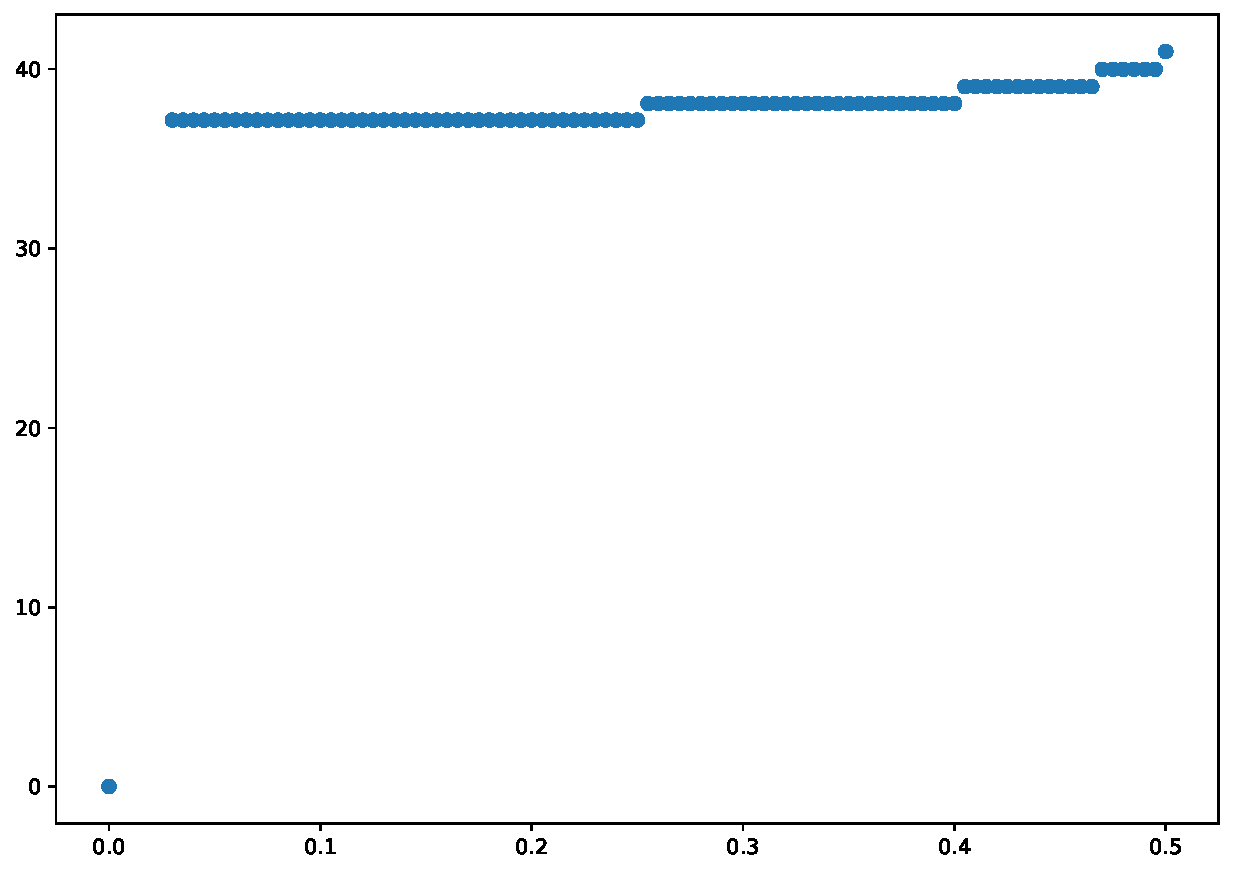
\includegraphics{Chapter6_files/figure-pdf/cell-14-output-2.pdf}

We again provide a program which does the same calculation using loops.
It is much slower. We use the same parametrs and preamble as before and
just outline the steps. As in the binomial model, we start at the last
date and build \(2n+1\) terminal stock prices. We also keep track of the
highest stock price which we exercise.

\begin{Shaded}
\begin{Highlighting}[]
\ImportTok{import}\NormalTok{ numpy }\ImportTok{as}\NormalTok{ np}
\ImportTok{import}\NormalTok{ matplotlib.pyplot }\ImportTok{as}\NormalTok{ plt}
\ImportTok{import}\NormalTok{ time}
\ImportTok{from}\NormalTok{ math }\ImportTok{import} \BuiltInTok{pow}\NormalTok{, exp, sqrt}
\CommentTok{\# parameters}
\CommentTok{\# number of steps}
\NormalTok{n }\OperatorTok{=} \DecValTok{100}
\CommentTok{\# interest rate}
\NormalTok{r }\OperatorTok{=} \FloatTok{.1}
\CommentTok{\# volatility}
\NormalTok{sig }\OperatorTok{=} \FloatTok{.2}
\CommentTok{\# Initial Stock Price}
\NormalTok{S0 }\OperatorTok{=} \DecValTok{42}
\CommentTok{\# Strike Price}
\NormalTok{K }\OperatorTok{=} \DecValTok{42}
\CommentTok{\# Maturity}
\NormalTok{T }\OperatorTok{=} \FloatTok{0.5}

\CommentTok{\# calculate parameters for trinomial model}
\NormalTok{dt }\OperatorTok{=}\NormalTok{ T}\OperatorTok{/}\NormalTok{n}
\NormalTok{a }\OperatorTok{=}\NormalTok{ np.exp(r}\OperatorTok{*}\NormalTok{dt)}
\NormalTok{u }\OperatorTok{=}\NormalTok{ np.exp(sig}\OperatorTok{*}\NormalTok{np.sqrt(}\DecValTok{3}\OperatorTok{*}\NormalTok{dt))}
\NormalTok{d }\OperatorTok{=} \DecValTok{1}\OperatorTok{/}\NormalTok{u}
\NormalTok{pu }\OperatorTok{=} \DecValTok{1}\OperatorTok{/}\DecValTok{6} \OperatorTok{+}\NormalTok{ np.sqrt(dt}\OperatorTok{/}\NormalTok{(}\DecValTok{12}\OperatorTok{*}\NormalTok{sig}\OperatorTok{**}\DecValTok{2}\NormalTok{))}\OperatorTok{*}\NormalTok{(r }\OperatorTok{{-}}\NormalTok{ sig}\OperatorTok{**}\DecValTok{2}\OperatorTok{/}\DecValTok{2}\NormalTok{)}
\NormalTok{pm }\OperatorTok{=} \DecValTok{2}\OperatorTok{/}\DecValTok{3}
\NormalTok{pd }\OperatorTok{=} \DecValTok{1} \OperatorTok{{-}}\NormalTok{ pu }\OperatorTok{{-}}\NormalTok{ pm}
\CommentTok{\# Build vector of ending values}
\CommentTok{\# and prices for which put is exercised}
\NormalTok{ex }\OperatorTok{=}\NormalTok{ np.zeros(n}\OperatorTok{+}\DecValTok{1}\NormalTok{)}
\NormalTok{S }\OperatorTok{=}\NormalTok{ np.zeros(}\DecValTok{2}\OperatorTok{*}\NormalTok{n}\OperatorTok{+}\DecValTok{1}\NormalTok{)}
\NormalTok{AP }\OperatorTok{=}\NormalTok{ np.zeros(}\DecValTok{2}\OperatorTok{*}\NormalTok{n}\OperatorTok{+}\DecValTok{1}\NormalTok{)}

\ControlFlowTok{for}\NormalTok{ j }\KeywordTok{in} \BuiltInTok{range}\NormalTok{(}\DecValTok{2}\OperatorTok{*}\NormalTok{n}\OperatorTok{+}\DecValTok{1}\NormalTok{):}
\NormalTok{    S[j] }\OperatorTok{=}\NormalTok{ S0}\OperatorTok{*}\NormalTok{u}\OperatorTok{**}\NormalTok{(j}\OperatorTok{{-}}\NormalTok{n)}
\NormalTok{    AP[j] }\OperatorTok{=} \BuiltInTok{max}\NormalTok{(K}\OperatorTok{{-}}\NormalTok{S[j],}\DecValTok{0}\NormalTok{)}
    \ControlFlowTok{if}\NormalTok{ AP[j]}\OperatorTok{\textgreater{}}\DecValTok{0}\NormalTok{:}
\NormalTok{        ex[n] }\OperatorTok{=}\NormalTok{ S[j]}
\end{Highlighting}
\end{Shaded}

We then move backwards. There are two loops. The inner loop builds the
stock price, the value, and exercise boundary at each time and the outer
loop moves backwards in time.

\begin{Shaded}
\begin{Highlighting}[]
\ControlFlowTok{for}\NormalTok{ i }\KeywordTok{in} \BuiltInTok{range}\NormalTok{(n):}
\NormalTok{    S }\OperatorTok{=}\NormalTok{ np.zeros(}\DecValTok{2}\OperatorTok{*}\NormalTok{(n}\OperatorTok{{-}}\NormalTok{i}\OperatorTok{{-}}\DecValTok{1}\NormalTok{)}\OperatorTok{+}\DecValTok{1}\NormalTok{)}
\NormalTok{    P }\OperatorTok{=}\NormalTok{ np.zeros(}\DecValTok{2}\OperatorTok{*}\NormalTok{(n}\OperatorTok{{-}}\NormalTok{i}\OperatorTok{{-}}\DecValTok{1}\NormalTok{)}\OperatorTok{+}\DecValTok{1}\NormalTok{)}
\NormalTok{    PP }\OperatorTok{=}\NormalTok{ np.zeros(}\DecValTok{2}\OperatorTok{*}\NormalTok{(n}\OperatorTok{{-}}\NormalTok{i}\OperatorTok{{-}}\DecValTok{1}\NormalTok{)}\OperatorTok{+}\DecValTok{1}\NormalTok{)}
    \ControlFlowTok{for}\NormalTok{ j }\KeywordTok{in} \BuiltInTok{range}\NormalTok{(}\DecValTok{2}\OperatorTok{*}\NormalTok{(n}\OperatorTok{{-}}\NormalTok{i}\OperatorTok{{-}}\DecValTok{1}\NormalTok{)}\OperatorTok{+}\DecValTok{1}\NormalTok{):}
\NormalTok{        S[j] }\OperatorTok{=}\NormalTok{ S0}\OperatorTok{*}\NormalTok{u}\OperatorTok{**}\NormalTok{(j}\OperatorTok{{-}}\NormalTok{(n}\OperatorTok{{-}}\NormalTok{i}\OperatorTok{{-}}\DecValTok{1}\NormalTok{))}
        \CommentTok{\#}
        \CommentTok{\# P calculates the value of early exercise}
\NormalTok{        P[j] }\OperatorTok{=} \BuiltInTok{max}\NormalTok{(K}\OperatorTok{{-}}\NormalTok{S[j],}\DecValTok{0}\NormalTok{)}
        \CommentTok{\#}
        \CommentTok{\# PP calculates value of waiting using payoffs}
        \CommentTok{\# from next period}
\NormalTok{        PP[j] }\OperatorTok{=}\NormalTok{ (pu}\OperatorTok{*}\NormalTok{AP[j}\OperatorTok{+}\DecValTok{2}\NormalTok{] }\OperatorTok{+}\NormalTok{ pm}\OperatorTok{*}\NormalTok{AP[j}\OperatorTok{+}\DecValTok{1}\NormalTok{] }\OperatorTok{+}\NormalTok{ pd}\OperatorTok{*}\NormalTok{AP[j])}\OperatorTok{/}\NormalTok{a}
        \CommentTok{\#}
        \CommentTok{\# AP is the max of ealry exercise and waiting}
\NormalTok{        AP[j] }\OperatorTok{=} \BuiltInTok{max}\NormalTok{(P[j],PP[j])}
        \CommentTok{\#}
        \CommentTok{\# ex is price where early exercise is optimal}
        \ControlFlowTok{if}\NormalTok{ P[j] }\OperatorTok{\textgreater{}}\NormalTok{ PP[j]:}
\NormalTok{            ex[n}\OperatorTok{{-}}\NormalTok{i] }\OperatorTok{=}\NormalTok{ S[j]}

\BuiltInTok{print}\NormalTok{(}\StringTok{\textquotesingle{}The American put price is =\textquotesingle{}}\NormalTok{, AP[}\DecValTok{0}\NormalTok{])            }
\CommentTok{\# plot the exercise boundary}
\NormalTok{plt.figure(figsize}\OperatorTok{=}\NormalTok{(}\DecValTok{10}\NormalTok{,}\DecValTok{7}\NormalTok{))}
\NormalTok{plt.scatter(dt}\OperatorTok{*}\NormalTok{np.arange(n}\OperatorTok{+}\DecValTok{1}\NormalTok{),ex)            }
\end{Highlighting}
\end{Shaded}

\begin{verbatim}
The American put price is = 1.6396310315369165
\end{verbatim}

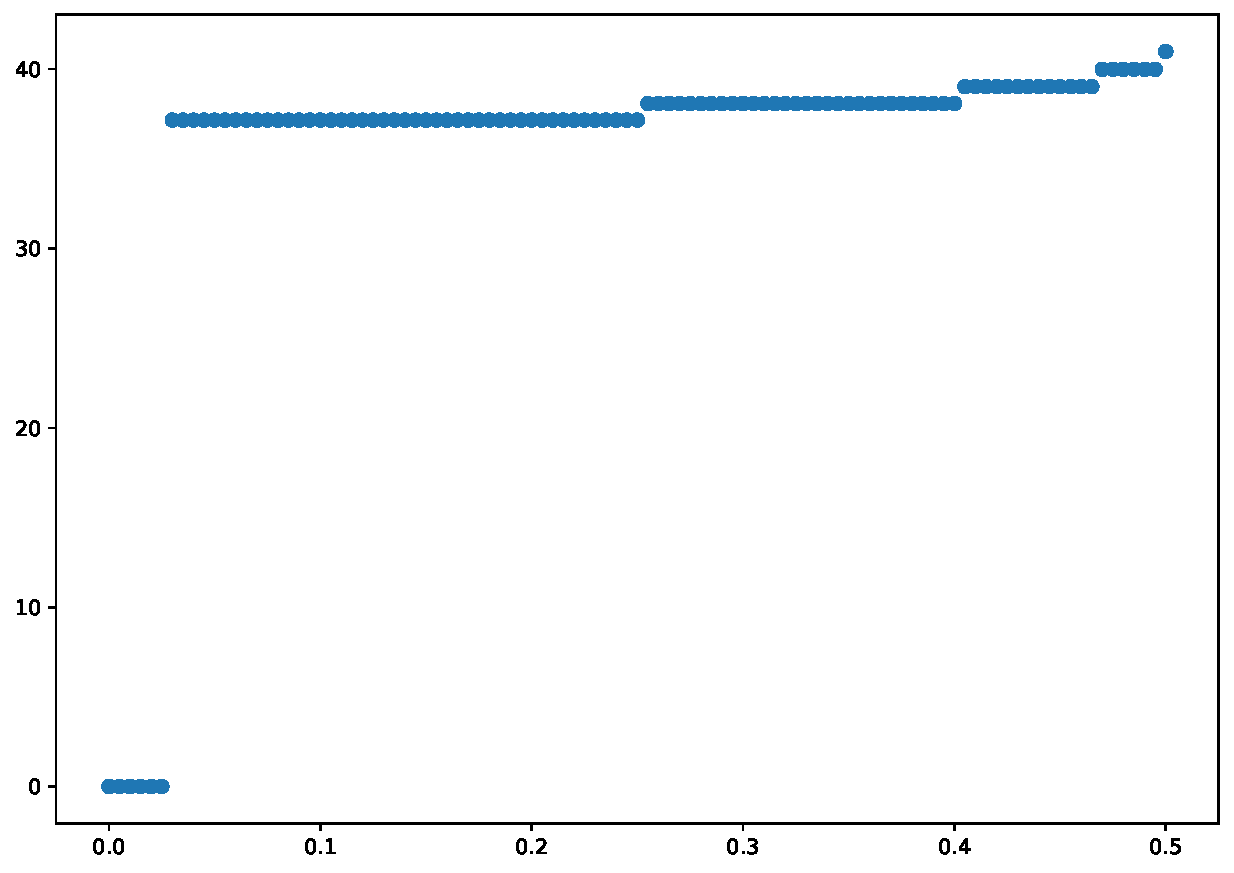
\includegraphics{Chapter6_files/figure-pdf/cell-16-output-2.pdf}

\section{Accelerating Binomial
Convergence}\label{accelerating-binomial-convergence}

Broadie and Detemple (Broadie and Detemple 1997) show that a modified
binomial model is a quite efficient way to value American put options.
They modify the binomial model as follows: (i) the Black-Scholes formula
is used to value the option at the penultimate date, and (ii) Richardson
extrapolation is used to estimate what the option value would be with an
infinite number of periods.

If an option is not exercised at date \(N-1\) in an \(N\)--period
binomial model (i.e., one date from the end), then, because in the
binomial model there are no further opportunities for early exercise,
the American option at date \(N-1\) is equivalent to a European option
at that date. The value of a European option is given by the
Black-Scholes formula. Therefore, the estimate of the option value can
be improved by replacing

\begin{verbatim}
PutV(j) = max(S-K, dpd*PutV(j)+dpu*PutV(j+1))
\end{verbatim}

with

\begin{verbatim}
PutV(j) = max(S-K,Black_Scholes_Put(S,K,r,sigma,q,dt))
\end{verbatim}

at date \(N-1\) (of course this also means that we do not need to
compute the intrinsic value at date \(N\)). This idea can be effectively
used in binomial valuation of any option for which there is a
closed-form solution (like the Black-Scholes formula) for the value of
the corresponding European option in a continuous-time model.

Broadie and Detemple combine the use of the Black-Scholes formula at
date \(N-1\) with \index{Richardson extrapolation} Richardson
extrapolation. Richardson extrapolation is a method that may improve the
efficiency of any algorithm by extrapolating to the limit. In the case
of a binomial model, the idea is to extrapolate the values calculated
for different numbers of periods (different \(N\)'s) to try to estimate
the value for \(N=\infty\).

It is easier to work with convergence to zero than convergence to
infinity, so define \(x=1/N\). For any value of \(N\), the binomial
model will return a value, which is an estimate of the option value and
which we denote as \(y=f(x)\). We would like to know the value at
\(N=\infty\), which in this notation is \(f(0)\). Of course, we cannot
calculate \(f(0)\), because we do not know the function \(f\), but we
can approximate \(f\) by a known function \(g\) and then estimate
\(f(0)\) by \(g(0)\).

A linear approximation is the simplest and is shown by Broadie and
Detemple to be quite effective. For a linear approximation, we would
take \[g(x) = a + bx\] for parameters \(a\) and \(b\) to be determined.
We can input values \(N_1\) and \(N_2 = 2N_1\) for the number of
periods, run the binomial model for each, set \(x_i=1/N_i\), and define
\(y_i=f(x_i)\) to be the value of the option returned by the binomial
model when the number of periods is \(N_i\). Then we force
\(g(x_i)=f(x_i)\) for \(i=1,2\) by solving the equations
\[y_i=a + bx_i\] for \(a\) and \(b\). Of course, \(g(0) = a\), so we
will return the constant \(a\) as our estimate of \(f(0)\). This is
simpler than it may appear---we put
\begin{equation*}\begin{array}{rclcl}
y_1 &= &a + bx_1 &= &a+2bx_2\;,\\
y_2 &= & &  & a + bx_2 \;,
\end{array}\end{equation*} and subtracting gives us \(y_1-y_2 = bx_2\),
which implies from the bottom equation that \(a = 2y_2-y_1\). We can
think of \(N_2\) as being the number of periods we want to use in the
binomial model, in which case \(y_2\) would be our estimate of the
option value. Richardson extrapolation here means also running the
binomial model for half as many periods (\(N_1 = N_2/2\)) and adding the
difference of the estimates \(y_2-y_1\) to the estimate \(y_2\).

Richardson extrapolation can be viewed as cancelling the first-order
term in the Taylor series expansion of \(f\). We have \begin{align*}
y_1 = f(x_1) &= f(0) + f'(0)x_1 + \text{higher order terms} \\
& = f(0) + 2f'(0)x_2 + \text{higher order terms}\;,\\
y_2 = f(x_2) &= f(0) + f'(0)x_2 + \text{higher order terms}\;.
\end{align*} \noindent This implies
\[2y_2-y_1 = f(0) + \text{difference of higher order terms}\;.\] Having
eliminated the first-order term, one can hope to obtain a closer
approximation to \(f(0)\).

We now show hot to implement this in Pyhton.\\
First we create a binomial valuation program that replaces (i)
calculation of the intrinsic value at maturity and (ii) calculation of
the value at the penultimate date as the larger of intrinsic value and
the discounted value at maturity with (iii) calculation of the value at
the penultimate date as the larger of intrinsic value and the
Black-Scholes value of a European option with one period to maturity.

\begin{Shaded}
\begin{Highlighting}[]
\CommentTok{\# uses blackscholes(S0, K, r, q, sig, T, call = False)}

\KeywordTok{def}\NormalTok{ binomialbd(n,r,sig,S0,y,K,T):}

    \CommentTok{\# parameters}
    \CommentTok{\# number of steps}
    \CommentTok{\#n }
    \CommentTok{\# interest rate}
    \CommentTok{\#r }
    \CommentTok{\# volatility}
    \CommentTok{\#sig }
    \CommentTok{\# Initial Stock Price}
    \CommentTok{\#S0}
    \CommentTok{\# Strike Price}
        \CommentTok{\#K }
    \CommentTok{\# Maturity}
    \CommentTok{\#T }
    \CommentTok{\# dividend yield}
    \CommentTok{\# y}

    \CommentTok{\# calculate parameters for binomial model}
\NormalTok{    dt }\OperatorTok{=}\NormalTok{ T}\OperatorTok{/}\NormalTok{n}
\NormalTok{    delt }\OperatorTok{=}\NormalTok{ np.exp(}\OperatorTok{{-}}\NormalTok{y}\OperatorTok{*}\NormalTok{dt)}
\NormalTok{    a }\OperatorTok{=}\NormalTok{ np.exp(r}\OperatorTok{*}\NormalTok{dt) }\OperatorTok{*}\NormalTok{ delt}
\NormalTok{    u }\OperatorTok{=}\NormalTok{ np.exp(sig}\OperatorTok{*}\NormalTok{np.sqrt(dt))}
\NormalTok{    d }\OperatorTok{=} \DecValTok{1}\OperatorTok{/}\NormalTok{u}
\NormalTok{    pu }\OperatorTok{=}\NormalTok{ (a}\OperatorTok{{-}}\NormalTok{d)}\OperatorTok{/}\NormalTok{(u}\OperatorTok{{-}}\NormalTok{d)}
\NormalTok{    pd }\OperatorTok{=} \DecValTok{1}\OperatorTok{{-}}\NormalTok{pu}
    \CommentTok{\# Build vector of ending values}
    \CommentTok{\# }
    
\NormalTok{    S }\OperatorTok{=}\NormalTok{ np.zeros(n)}
\NormalTok{    AP }\OperatorTok{=}\NormalTok{ np.zeros(n)}
    
    \CommentTok{\# Build vector of ending values}
    \CommentTok{\# at the next to last date (penultimate date)}
\NormalTok{    vec }\OperatorTok{=}\NormalTok{ np.arange(n)}
\NormalTok{    vec1 }\OperatorTok{=}\NormalTok{ np.ones(n)}

\NormalTok{    S }\OperatorTok{=}\NormalTok{ S0 }\OperatorTok{*}\NormalTok{ u}\OperatorTok{**}\NormalTok{(}\DecValTok{2}\OperatorTok{*}\NormalTok{vec }\OperatorTok{{-}}\NormalTok{ (n}\OperatorTok{{-}}\DecValTok{1}\NormalTok{)}\OperatorTok{*}\NormalTok{vec1)}

\NormalTok{    AP }\OperatorTok{=}\NormalTok{ np.maximum(K}\OperatorTok{{-}}\NormalTok{S,blackscholes(S, K, r, q, sig, dt, call }\OperatorTok{=} \VariableTok{False}\NormalTok{))}
    
    
    \CommentTok{\# Backward recursion in the loop}
    \ControlFlowTok{for}\NormalTok{ i }\KeywordTok{in} \BuiltInTok{range}\NormalTok{(n}\OperatorTok{{-}}\DecValTok{1}\NormalTok{):}
\NormalTok{        vec }\OperatorTok{=}\NormalTok{ np.arange(n}\OperatorTok{{-}}\NormalTok{i}\OperatorTok{{-}}\DecValTok{1}\NormalTok{)}
\NormalTok{        vec1 }\OperatorTok{=}\NormalTok{ np.ones(n}\OperatorTok{{-}}\NormalTok{i}\OperatorTok{{-}}\DecValTok{1}\NormalTok{)}
        \CommentTok{\# Possible Stock prices at times{-}i period}
\NormalTok{        S }\OperatorTok{=}\NormalTok{ S0 }\OperatorTok{*}\NormalTok{ u}\OperatorTok{**}\NormalTok{(}\DecValTok{2}\OperatorTok{*}\NormalTok{vec}\OperatorTok{{-}}\NormalTok{(n}\OperatorTok{{-}}\NormalTok{i}\OperatorTok{{-}}\DecValTok{1}\NormalTok{)}\OperatorTok{*}\NormalTok{vec1}\OperatorTok{+}\DecValTok{1}\NormalTok{)}
    
    \CommentTok{\#     S = S0 * u**(2*vec{-}(n{-}i))}
        \CommentTok{\# P calculates the value of early exercise}
\NormalTok{        P }\OperatorTok{=}\NormalTok{ np.maximum(K}\OperatorTok{*}\NormalTok{vec1 }\OperatorTok{{-}}\NormalTok{ S, }\DecValTok{0}\NormalTok{)}
        \CommentTok{\# PP calculates value of waiting using payoffs from next period}
\NormalTok{        PP }\OperatorTok{=}\NormalTok{ (pu}\OperatorTok{*}\NormalTok{AP[}\DecValTok{1}\NormalTok{:(n}\OperatorTok{{-}}\NormalTok{i)] }\OperatorTok{+}\NormalTok{ pd}\OperatorTok{*}\NormalTok{AP[}\DecValTok{0}\NormalTok{:(n}\OperatorTok{{-}}\NormalTok{i}\OperatorTok{{-}}\DecValTok{1}\NormalTok{)])}\OperatorTok{/}\NormalTok{a}
        \CommentTok{\# AP is the max of ealry exercise and waiting}
\NormalTok{        AP }\OperatorTok{=}\NormalTok{ np.maximum(P,PP)}
        

    
    
    
    \ControlFlowTok{return}\NormalTok{ AP[}\DecValTok{0}\NormalTok{]          }
\end{Highlighting}
\end{Shaded}

Now we create a program that uses Richardson extrapolation from a
binomial model with N periods and a binomial model with N/2 periods to
estimate the value from a binomial model with an infinite number of
periods. We use the previous program as our binomial model. The number
of time steps \(n\) must be even so \(n/2\) is an integer. In the
following we initally use \(n=20\), which is smaller than the the number
of steps in the previous binomial american option routines.

\begin{Shaded}
\begin{Highlighting}[]
\ImportTok{import}\NormalTok{ numpy }\ImportTok{as}\NormalTok{ np}
\ImportTok{import}\NormalTok{ matplotlib.pyplot }\ImportTok{as}\NormalTok{ plt}
\ImportTok{import}\NormalTok{ time}
\ImportTok{from}\NormalTok{ math }\ImportTok{import} \BuiltInTok{pow}\NormalTok{, exp, sqrt}


\CommentTok{\#inputs}
\CommentTok{\#number of steps= n; must be an even number}
\NormalTok{n}\OperatorTok{=}\DecValTok{20}
\CommentTok{\# interest rate}
\NormalTok{r}\OperatorTok{=}\FloatTok{.1}
\CommentTok{\# volatility}
\NormalTok{sig}\OperatorTok{=}\FloatTok{.2}
\CommentTok{\# initial stock price}
\NormalTok{S0}\OperatorTok{=}\DecValTok{42}
\CommentTok{\# dividend yield}
\NormalTok{y}\OperatorTok{=}\DecValTok{0}
\CommentTok{\# Strike price }
\NormalTok{K}\OperatorTok{=}\DecValTok{42}
\CommentTok{\# expiration}
\NormalTok{T}\OperatorTok{=}\FloatTok{0.5}

\ControlFlowTok{if} \DecValTok{2}\OperatorTok{*}\BuiltInTok{int}\NormalTok{(n}\OperatorTok{/}\DecValTok{2}\NormalTok{) }\OperatorTok{==}\NormalTok{ n:}

\NormalTok{    y2}\OperatorTok{=}\NormalTok{binomialbd(n,r,sig,S0,y,K,T)}
\NormalTok{    y1}\OperatorTok{=}\NormalTok{binomialbd(}\BuiltInTok{int}\NormalTok{(n}\OperatorTok{/}\DecValTok{2}\NormalTok{),r,sig,S0,y,K,T)}
    
\NormalTok{    extrapolate}\OperatorTok{=} \DecValTok{2}\OperatorTok{*}\NormalTok{y2}\OperatorTok{{-}}\NormalTok{y1}
    \BuiltInTok{print}\NormalTok{(}\StringTok{\textquotesingle{}The extrapolated value=\textquotesingle{}}\NormalTok{,extrapolate)}

\ControlFlowTok{else}\NormalTok{:}
    \BuiltInTok{print}\NormalTok{(}\StringTok{\textquotesingle{}n must be even you big dummy!!\textquotesingle{}}\NormalTok{)   }
\end{Highlighting}
\end{Shaded}

\begin{verbatim}
The extrapolated value= 1.6495917266169138
\end{verbatim}

\section{Exercises}\label{exercises-4}

\begin{exercise}[]\protect\hypertarget{exr-nolabel}{}\label{exr-nolabel}

Consider an at-the-money European call option on a non-dividend-paying
stock with six months to maturity. Take the initial stock price to be
\$50, the interest rate to be 5\% and \$\sigma=\$30\%. Compute the value
in a binomial model with \(N=10, 11, \ldots, 20\) and plot the values
against \(N\). Plot your results. Is convergence monotone?

\end{exercise}

\begin{exercise}[]\protect\hypertarget{exr-nolabel}{}\label{exr-nolabel}

Consider the same option as in the previous problem. Roughly what value
of \(N\) is needed to get penny accuracy? (To evaluate the accuracy,
compare the price to the price given by the Black-Scholes formula.)

\end{exercise}

\begin{exercise}[]\protect\hypertarget{exr-nolabel}{}\label{exr-nolabel}

Repeat the two previous problems only instead of the Cox, Ross
Rubenstein model, use the Jarrow Rudd model.

\end{exercise}

\begin{exercise}[]\protect\hypertarget{exr-nolabel}{}\label{exr-nolabel}

The early exercise premium \index{early exercise premium} is the
difference between the value of an American option and the value of a
European option with the same parameters. Compute the early exercise
premium for an American put and various values for the interest rate,
exercise price, and stock parameters. Under what circumstances is the
early exercise premium relatively large?

\end{exercise}

\begin{exercise}[]\protect\hypertarget{exr-nolabel}{}\label{exr-nolabel}

A shout option is an option where the holder is entitled to shout at any
time before the expiration of the option. Upon shouting, the holder
receives the immediate exercise value paid at expiration, plus an at the
money option with the same expiration as the original option. The payoff
to this option if the holder shouts at time \(\tau\) is thus given as
\(\max(0, S(\tau)-K, S(T)-K )\) where \(K\) is the original strike
price.\\
1) Show that it is better to shout at some time where \(S(\tau)>K\) than
to never shout at all. 2) Modify the code for an American put to find
the optimal exercise boundary for a shout option. Hint: The payoffs on
the last nodes of the tree are simply \((S_T - K)^+\). Then work
backwards. The `immediate exercise value' which is the present value of
\(S(t)-K\), (\(e^{-r(T-t)} (S(t) -K)\)) plus the Black Scholes value
(use a python function) of an at the money option with expiration
\(T-t\). Choose the maximum of these values at each node. For each time
store the highest price at which you exersize. The first node (time 0)
then gives the price. Plot the exercise boundary.

\end{exercise}

\bookmarksetup{startatroot}

\chapter{Foreign Exchange}\label{sec-c_foreignexchange}

We will see in this chapter how to apply the Black-Scholes formulas to
value currency options and options on foreign assets. We will also
discuss currency forwards and futures, quanto forwards, and return
swaps.

For concreteness, we will call one currency the domestic currency and
the other the foreign currency. Let \(X(t)\) denote the exchange rate at
time \(t\) measured in units of the domestic currency per unit of the
foreign currency. Exchange rates can be confusing, because we can look
at them from the perspective of either currency, so it may help to keep
in mind that \(X(t)\) here means the price of a unit of the foreign
currency, just as we might consider the price of a stock. When we speak
of the cost or value of something without specifying the currency, it
should be understood to be the domestic currency that we mean. If \(S\)
is the price of a foreign asset, denominated in units of the foreign
currency, we can convert it into a domestic asset price simply by
multiplying by the exchange rate: \(X(t)S(t)\) is the price of the
asset, denominated in the domestic currency. For example, if the
domestic currency is dollars and the foreign currency is yen, then \(S\)
is in units of yen and \(X\) is units of dollars per unit of yen, so
\(XS\) is in units of dollars.

Throughout the chapter, we will maintain assumptions similar to the
Black-Scholes assumptions. There is a foreign asset with price \(S\) in
the foreign currency. It has a constant dividend yield \(q\) and a
constant volatility \(\sigma_s\). The exchange rate has a constant
volatility \(\sigma_x\) and a constant correlation \(\rho\) with the
foreign asset. There is a domestic risk-free asset with constant
interest rate \(r\) and a foreign risk-free asset with constant interest
rate \(r_f\). The term risk free means of course that they are risk-free
in their respective currencies. For example, an investment in the
foreign risk-free asset is not risk free to a domestic investor, because
of exchange rate risk.

\section{\texorpdfstring{Currency
Options\index{currency option}}{Currency Options}}\label{currency-options}

A European call option on the exchange rate \(X\) pays
\(\max(0,X(T)-K)\) at its maturity \(T\), where \(K\) is the strike
price (in domestic currency). The underlying asset should be regarded as
the foreign risk-free asset, the domestic price of which fluctuates with
the exchange rate. An investment in the foreign risk-free asset grows
via reinvestment of interest at rate \(r_f\), just as the number of
shares held of a stock grows via reinvestment of dividends at rate
\(q\), if \(q\) is its constant dividend yield. In particular, the cost
at date\textasciitilde0 of obtaining one unit of foreign currency at
date \(T\) is the cost at date 0 of \(\mathrm{e}^{-r_fT}\) units of
foreign currency, which is \(\mathrm{e}^{-r_fT}X(0)\). Thus, the
exchange rate is analogous to a stock price, with the foreign risk-free
rate being its dividend yield. This means we can apply the Black-Scholes
formulas to value currency calls and puts:

\begin{tcolorbox}[enhanced jigsaw, leftrule=.75mm, colback=white, colframe=quarto-callout-tip-color-frame, breakable, title={Tip}, titlerule=0mm, bottomrule=.15mm, toprule=.15mm, arc=.35mm, left=2mm, toptitle=1mm, bottomtitle=1mm, rightrule=.15mm, colbacktitle=quarto-callout-tip-color!10!white, opacityback=0, coltitle=black, opacitybacktitle=0.6]

Calls and puts on foreign currency can be valued by the Black-Scholes
formulas with inputs \(X(0) =\) initial asset price, \(r =\) risk-free
rate, \(\sigma_x =\) volatility, and \(r_f =\) dividend yield.

\end{tcolorbox}

\section{Options on Foreign Assets Struck in Foreign
Currency}\label{sec-s_foreignstrike}

An option on a foreign asset, with the strike price defined in the
foreign currency, can be priced with the Black-Scholes formula, assuming
the volatility and dividend yields of the asset are constant and that
the (foreign) interest rate is constant. This must be true, because we
did not need to specify the currency (dollars, yen, etc.) when deriving
the Black-Scholes formula. The value given by the Black-Scholes formula
is in the same currency as the asset. To obtain a value in domestic
currency for an option on a foreign asset, we simply multiply the
Black-Scholes formula by the current exchange rate.

\section{Options on Foreign Assets Struck in Domestic
Currency}\label{sec-s_domesticstrike}

A call option on a foreign asset with domestic strike price \(K\) on the
foreign asset with price \(S\) pays \[\max(X(T)S(T)-K,0)\] at its
maturity \(T\). The underlying price \(X(T)S(T)\) is the value in
domestic currency of the portfolio that with starts with
\(\mathrm{e}^{-qT}\) units of the asset and reinvests dividends until
date \(T\). Thus, we can use the Black-Scholes formula to value it,
taking the initial asset price to be \(\mathrm{e}^{-qT}X(0)S(0)\) and
the dividend rate to be zero (or taking the initial asset price to be
\(X(0)S(0)\) and the dividend rate to be \(q\)). The volatility that
should be input into the Black-Scholes formula is the volatility of the
domestic currency price \(\mathrm{e}^{-q(T-t)}X(t)S(t)\), which is the
same as the volatility of \(X(t)S(t)\).\\
According to Equation~\ref{eq-volatilityproduct}, the volatility of the
domestic currency price \(XS\) is
\begin{equation}\phantomsection\label{eq-foreignoptiondomcurrencyvol}{
\sigma = \sqrt{\sigma_x^2+\sigma_s^2+2\rho\sigma_x\sigma_s}\;.
}\end{equation}

We conclude:

\begin{tcolorbox}[enhanced jigsaw, leftrule=.75mm, colback=white, colframe=quarto-callout-tip-color-frame, breakable, title={Tip}, titlerule=0mm, bottomrule=.15mm, toprule=.15mm, arc=.35mm, left=2mm, toptitle=1mm, bottomtitle=1mm, rightrule=.15mm, colbacktitle=quarto-callout-tip-color!10!white, opacityback=0, coltitle=black, opacitybacktitle=0.6]

Calls and puts on foreign assets struck in domestic currency can be
valued by the Black-Scholes formulas with inputs \(X(0)S(0) =\) initial
price, \(r =\) risk-free rate,
Equation~\ref{eq-foreignoptiondomcurrencyvol} = volatility, \(q =\)
dividend yield.

\end{tcolorbox}

\section{Currency Forwards and Futures}\label{sec-s_currencyforwards}

Consider a forward contract maturing at some date \(T\) on one unit of
foreign currency. In keeping with our convention for options, we will
always assume (without loss of generality) that a forward contract is
written on a single unit of currency. Let \(F(t)\) denote the forward
price (in domestic currency) at date \(t\leq T\). This means that
someone who purchases (goes long) the contract at date \(t\) will
receive a unit of foreign currency, worth \(X(T)\), at date \(T\) and
must pay \(F(t)\) at date \(T\). \index{forward contract} The value of
the long contract at date \(T\) is therefore \(X(T) - F(t)\). The value
at date \(T\) of a short contract initiated at date \(t\) is the
opposite: \(F(t)-X(T)\). Naturally, the forward price \(F(t)\) is called
the forward exchange rate. \index{forward exchange rate}

The deepest market for currency is the inter-bank forward market, but
futures contracts are also traded on exchanges. The difference between
forwards and futures is that futures are marked to market daily.
\index{futures contract} \index{marking to market} Thus, there are daily
cash flows with a futures contract, whereas the only cash flows on a
forward contract occur at the maturity of the forward. In both cases,
there is no cash flow at the time the contract is bought/sold, so its
market value is zero. In Section~\ref{sec-s_futuresforwards} we will
discuss futures contracts further. In particular, we will show, assuming
continuous marking to market, that if there is a constant (domestic)
risk-free rate---or, more generally, if there is an instantaneous
risk-free rate that changes over time in a non-random way---then futures
prices must equal forward prices in the absence of arbitrage
opportunities. Thus, our assumptions in this chapter imply that currency
futures prices should equal currency forward prices. We will consider
currency forwards in the remainder of this section.

A forward contract on a traded asset can always be created synthetically
simply by buying the asset and holding it, using borrowed money to
finance the purchase and to finance any storage costs, assuming the
storage costs can be estimated in advance. \index{synthetic forward} If
the asset pays dividends or generates other positive cash flows, then we
do not need to purchase the entire amount covered by the forward
contract, because we can accumulate additional amounts of the asset by
reinvesting the dividends. There are no storage costs on currency and
its dividend yield is equal to the foreign risk-free rate. A forward
contract on one unit of foreign currency maturing at date \(T\) can be
created synthetically at date 0 by buying \(\mathrm{e}^{-r_fT}\) units
of foreign currency and borrowing the cost \(\mathrm{e}^{-r_fT}X(0)\) at
the domestic risk-free rate. This will lead to ownership of one unit of
foreign currency at date \(T\) and a liability, including interest, of
\(\mathrm{e}^{(r-r_f)T}X(0)\) at date \(T\). Thus, the forward price at
date 0 must be \(F(0) = \mathrm{e}^{(r-r_f)T}X(0)\); otherwise, one
could arbitrage by buying the forward and selling the synthetic forward,
or vice versa. More generally,

\begin{tcolorbox}[enhanced jigsaw, leftrule=.75mm, colback=white, colframe=quarto-callout-tip-color-frame, breakable, title={Tip}, titlerule=0mm, bottomrule=.15mm, toprule=.15mm, arc=.35mm, left=2mm, toptitle=1mm, bottomtitle=1mm, rightrule=.15mm, colbacktitle=quarto-callout-tip-color!10!white, opacityback=0, coltitle=black, opacitybacktitle=0.6]

The forward exchange rate at date \(t\), for a contract maturing at
\(T\), must be
\begin{equation}\phantomsection\label{eq-forwardexchangerate}{
F(t) = \mathrm{e}^{(r-r_f)(T-t)}X(t)\;.
}\end{equation}

\end{tcolorbox}

The relation Equation~\ref{eq-forwardexchangerate} is called covered
interest parity. \index{covered interest parity}The name stems from the
fact that an investment in one of the risk-free assets (foreign or
domestic) financed by borrowing in the other, with the currency risk
hedged (covered) by a forward contract, is certain to generate zero
value (otherwise, it would be an arbitrage opportunity).\^{}{[} A
relation analogous to covered interest parity holds for any forward
contract if the underlying asset has a constant dividend yield and
storage costs that are a constant proportion of the value of the units
stored. For commodities, the term dividend yield must be interpreted in
a broad sense, and is usually called convenience yield,
\index{convenience yield] because ownership of the physical asset may produce abnormal profits during temporary shortages, an advantage that is not obtained by owning a forward contract on the asset, just as dividends are not received by the owner of a forward contract.  Thus, one must consider the convenience of owning the physical asset as an advantage analogous to dividends.}

Suppose that one has made a commitment to pay a certain amount of
foreign currency (perhaps to a foreign manufacturer) at some date in the
future. The exchange rate risk that this commitment entails can
obviously be hedged by buying the currency forward. However, one can
also create a synthetic forward, by buying currency today and investing
it in the foreign risk-free asset. The cash outflow can be incurred
today, or it can be deferred by borrowing the cost of the currency at
the domestic risk-free rate. In the latter case, we have created a true
synthetic forward. In either case, we would call this a money market
hedge \index{money market hedge} because we have utilized the foreign
money market (risk-free asset) to create the hedge.

Later in this chapter we will construct replicating strategies for
various contracts using the foreign risk-free asset and the domestic
risk-free asset. One can interpret these replicating strategies as money
market hedges or synthetic currency forwards. In practice, it will often
be more convenient to use actual forwards rather than using the foreign
risk-free asset. Using actual currency forwards produces an equivalent
(given that we are not considering transaction costs) replicating
strategy. Here is, in abstract, the way we convert from money market
hedges to hedges using forwards. As we have discussed, \begin{align*}
\text{Long Currency Forward} &= \text{Long Synthetic Currency Forward} \\
&= \text{Long Foreign Risk-Free Asset} \\
&\qquad + \text{Short Domestic Risk-Free Asset}\;.
\end{align*} Subtracting a short position is the same as adding a long
position, so we can rearrange this as \begin{multline*}
\text{Long Currency Forward} + \text{Long Domestic Risk-Free Asset}\\=  \text{Long Foreign Risk-Free Asset} \; .
\end{multline*} Thus, an investment in the foreign risk-free asset can
be replaced in any replicating strategy by long currency forwards and an
investment in the domestic risk-free asset.

To be more precise about the sizes of the investments, consider
replacing a money market hedge with a forward hedge at some date \(t\)
prior to the maturity of the forward and analyze the replacement per
unit of the money market hedge (per unit of foreign currency invested in
the foreign risk-free asset). One unit of foreign currency invested in
the foreign risk-free asset at date \(t\) will grow to
\(\mathrm{e}^{r_f(T-t)}\) units by date \(T\). Thus, the corresponding
forward contract should be on \(\mathrm{e}^{r_f(T-t)}\) units of
currency. The value at date \(t\) of both sides of the above equation
should be the same, and the value of a forward contract at the date of
initiation is zero, so the investment in the domestic risk-free asset
should be the domestic currency equivalent of one unit of foreign
currency, which is the exchange rate \(X(t)\). Thus, we have

\begin{tcolorbox}[enhanced jigsaw, leftrule=.75mm, colback=white, colframe=quarto-callout-tip-color-frame, breakable, title={Tip}, titlerule=0mm, bottomrule=.15mm, toprule=.15mm, arc=.35mm, left=2mm, toptitle=1mm, bottomtitle=1mm, rightrule=.15mm, colbacktitle=quarto-callout-tip-color!10!white, opacityback=0, coltitle=black, opacitybacktitle=0.6]

\begin{multline}
 \text{$\mathrm{e}^{r_f(T-t)}$ Long Currency Forwards} \\+  \text{$X(t)$ Long in the Domestic Risk-Free Asset}\\
= \text{1 Unit of Foreign Currency Long in the Foreign Risk-Free Asset}\;.
\end{multline} \{\#eq-mmhedge\}

\end{tcolorbox}

To check this, consider holding the portfolios until date \(T\). As
explained in the first paragraph of this section, the currency forwards
will have value \(\mathrm{e}^{r_f(T-t)}[X(T)-F(t)]\), which by covered
interest parity is
\(\mathrm{e}^{r_f(T-t)}X(T)-\mathrm{e}^{r(T-t)}X(t)\). When we include
the long position in the domestic risk-free asset with accumulated
interest, the value at date \(T\) of the portfolio on the left-hand side
of \textbf{?@eq-mmhedge} is \(\mathrm{e}^{r_f(T-t)}X(T)\). On the other,
the right-hand side of \textbf{?@eq-mmhedge} with accumulated interest
will consist of \(\mathrm{e}^{r_f(T-t)}\) units of foreign currency,
also worth \(\mathrm{e}^{r_f(T-t)}X(T)\).

\section{Quantos}\label{sec-s_quantos}

A quanto \index{quanto} is a derivative written on a foreign asset the
value of which is converted to domestic currency at a fixed exchange
rate. In other words, the contract pays in the domestic currency and the
exchange rate is part of the contract. Such contracts are very useful
for investors who want to bet on foreign assets but do not want exposure
to exchange rate risk. Such an investor could simply buy the foreign
asset and hedge the currency risk by selling currency futures or
forwards, but doing so is a bit tricky because the amount of currency
that needs to be hedged depends on how well the foreign asset does.
Thus, quantos can be desirable contracts. Of course, when an investor
purchases a quanto, the problem of hedging the exchange rate risk has
simply been transferred to the seller. In this and the following
section, we will see how to value and how to replicate a contract that
pays the price of a foreign asset at some future date \(T\) with the
price translated into the domestic currency at a fixed exchange rate.
The replicating strategy is the strategy that would be followed by the
seller (or by an investor who wants to create a synthetic on his own).
Specifically, in this section we will determine the value at date 0 (in
domestic currency) of a contract that pays \(\bar{X}S(T)\) at date
\(T\), where \(\bar{X}\) is a fixed exchange rate. Later in the chapter,
we will consider quanto forwards and quanto options.

In addition to being practically useful, this contract is an excellent
example for demonstrating the methodology of pricing and hedging. The
best way to proceed in problems of this general type is to first value
the contract and then calculate the replicating strategy.\footnote{We
  did the same thing in Chapter~\ref{sec-c_blackscholes}}: we first
derived the Black-Scholes formula and then found the replicating
strategy (delta hedge) by differentiating the formula. As discussed in
Section~\ref{sec-s_introoptions}, valuation is simplified by choosing a
numeraire that will cancel the randomness in the contract payoff. Our
numeraire must be a non-dividend-paying (domestic) asset price, so we
can choose \(Z(t)=X(t)\mathrm{e}^{qt}S(t)\) to be the numeraire asset
price. This is the value in the domestic currency of a strategy that is
long one unit of the foreign asset at date 0 and which reinvests the
dividends of the asset into new shares. As we will see immediately,
using it as numeraire introduces randomness into the payoff through the
exchange rate, and that poses some complications. Applying our
fundamental pricing Equation~\ref{eq-formula}, the value of the contract
is

\[
Z(0) E^Z \left[\frac{\bar{X}S(T)}{Z(T)}\right] = \mathrm{e}^{-qT}X(0)S(0)E^Z \left[\frac{\bar{X}S(T)}{X(T)S(T)}\right]
\] \begin{equation}\phantomsection\label{eq-quanto}{
= \mathrm{e}^{-qT}\bar{X}S(0)E^Z \left[\frac{X(0)}{X(T)}\right]\;.
}\end{equation}

Now we need to evaluate \(E^Z[X(0)/X(T)]\), which is the expected growth
of \(1/X\) when \(Z\) is used as the numeraire. We will show that
\begin{equation}\phantomsection\label{eq-growthreciprocalX}{
E^Z \left[\frac{X(0)}{X(T)}\right] = \exp\left\{(r_f - r-\rho\sigma_x\sigma_s)T\right\}\;.
}\end{equation}

This implies:

\begin{tcolorbox}[enhanced jigsaw, leftrule=.75mm, colback=white, colframe=quarto-callout-tip-color-frame, breakable, title={Tip}, titlerule=0mm, bottomrule=.15mm, toprule=.15mm, arc=.35mm, left=2mm, toptitle=1mm, bottomtitle=1mm, rightrule=.15mm, colbacktitle=quarto-callout-tip-color!10!white, opacityback=0, coltitle=black, opacitybacktitle=0.6]

The value at date 0 of a contract that pays \(\bar{X}S(T)\) at date
\(T\), where \(\bar{X}\) is a fixed exchange rate and \(S\) is the
foreign price of an asset with a constant dividend yield \(q\), is
\begin{equation}\phantomsection\label{eq-quanto1}{
\exp\left\{(r_f - r-q-\rho\sigma_x\sigma_s)T\right\}\bar{X}S(0)\;.
}\end{equation}

\end{tcolorbox}

\begin{tcolorbox}[enhanced jigsaw, leftrule=.75mm, colback=white, colframe=quarto-callout-note-color-frame, breakable, title={Note}, titlerule=0mm, bottomrule=.15mm, toprule=.15mm, arc=.35mm, left=2mm, toptitle=1mm, bottomtitle=1mm, rightrule=.15mm, colbacktitle=quarto-callout-note-color!10!white, opacityback=0, coltitle=black, opacitybacktitle=0.6]

\#\#

We will now prove Equation~\ref{eq-growthreciprocalX}. The assumption
that \(S\) and \(X\) have constant volatilities and correlation means
that\\
\begin{align*}
\frac{\mathrm{d} X}{X} &= \mu_x\,\mathrm{d} t+\sigma_x\,\mathrm{d} B_x\;,\\
\frac{\mathrm{d} S}{S} &= \mu_s\,\mathrm{d} t+\sigma_s\,\mathrm{d} B_s\;,
\end{align*} for some (possibly random) \(\mu_x\) and \(\mu_s\), where
\(B_s\) and \(B_x\) are Brownian motions with correlation equal to
\(\rho\). From Ito's formula, we have \begin{align*}
\frac{\mathrm{d} Z}{Z} &= q\,\mathrm{d} t + \frac{\mathrm{d} (XS)}{XS}\\
&= \left(q+\mu_x +\mu_s+ \rho\sigma_x\sigma_s\right)\,\mathrm{d} t + \sigma_x\,\mathrm{d} B_x + \sigma_s\,\mathrm{d} B_s \\
&= \left(q+\mu_x +\mu_s+ \rho\sigma_x\sigma_s\right)\,\mathrm{d} t + \sigma\left(\frac{\sigma_x}{\sigma}\,\mathrm{d} B_x + \frac{\sigma_s}{\sigma}\,\mathrm{d} B_s\right) \\
&= \left(q+\mu_x +\mu_s+ \rho\sigma_x\sigma_s\right)\,\mathrm{d} t + \sigma\,\mathrm{d} B\;,
\end{align*} where we define \(\sigma\) in
Equation~\ref{eq-foreignoptiondomcurrencyvol} and \(B\) by \(B(0)=0\)
and
\[\mathrm{d} B = \frac{\sigma_x}{\sigma}\,\mathrm{d} B_x + \frac{\sigma_s}{\sigma}\,\mathrm{d} B_s\; .\]
As discussed in Section~\ref{sec-s_volatilities}, \(B\) is a Brownian
motion and \(\sigma\) is the volatility of \(Z\). Notice that the
correlation of \(X\) and \(Z\) is \begin{align*}
(\mathrm{d} B)(\mathrm{d} B_x) &= \left(\frac{\sigma_x}{\sigma}\,\mathrm{d} B_x + \frac{\sigma_s}{\sigma}\,\mathrm{d} B_s\right)(\mathrm{d} B_x)\\
&= \frac{\sigma_x + \rho\sigma_s}{\sigma}\,\mathrm{d} t\;.
\end{align*} Now we use Equation~\ref{eq-other11} in
Section~\ref{sec-s_girsanov} which gives the drift of an asset when
another risky asset is used as the numeraire. We use \(Z\) as the
numeraire and \(X\) as the other asset, regarding \(X\) as the domestic
price of an asset with dividend yield \(r_f\) as before. Therefore, we
substitute \(r_f\) for \(q\) in Equation~\ref{eq-other11}, substitute
\(\sigma\) for the volatility of the numeraire asset price, substitute
\(\sigma_x\) for the volatility of the other asset, and substitute
\((\sigma_x+\rho\sigma_s)/\sigma\) for their correlation. This yields
\[\frac{\mathrm{d} X}{X} = \left(r-r_f+\sigma_x^2+\rho\sigma_x\sigma_s\right)\,\mathrm{d} t + \sigma_x\,\mathrm{d} B^*_x\; ,\]
where \(B^*_x\) is a Brownian motion when \(Z\) is the numeraire.\\
Now we apply Ito's formula for ratios to obtain \begin{align*}
\frac{\mathrm{d} (1/X)}{1/X} &= -\frac{\mathrm{d} X}{X} + \left(\frac{\mathrm{d} X}{X}\right)^2\\
&= \left(r_f-r-\rho\sigma_x\sigma_s\right)\,\mathrm{d} t + \sigma_x\,\mathrm{d} B^*_x\;.
\end{align*} This implies that \(1/X\) is a geometric Brownian motion
with growth rate \(r_f-r-\rho\sigma_x\sigma_s\), from which
Equation~\ref{eq-growthreciprocalX} follows.

\end{tcolorbox}

\section{Replicating Quantos}\label{sec-s_replicatingquantos}

The assets we will use to replicate the payoff \(\bar{X}S(T)\) are the
foreign asset with price \(S\), the foreign risk-free asset, and the
domestic risk-free asset. At the end of this section, we will explain
how to replace the foreign risk-free asset with currency forwards, as
discussed in Section~\ref{sec-s_currencyforwards}. Before beginning the
calculations, we can make the following intuitive observations:

\begin{itemize}
\tightlist
\item
  The payoff \(\bar{X}S(T)\) has exposure to the foreign asset price
  \(S\), so the replicating portfolio must be long the foreign asset.\\
\item
  The payoff \(\bar{X}S(T)\) has no exposure to the exchange rate, so
  the replicating portfolio cannot have any exposure to the exchange
  rate either. Thus, the long position in the foreign risky asset must
  be offset by an equal short position in the foreign risk-free asset.\\
\item
  As a result of the previous observation, the value of the replicating
  portfolio, displayed in Equation~\ref{eq-quanto1}, will equal the
  investment in the domestic risk-free asset.
\end{itemize}

Consequently, our real task is to compute the number of shares of the
foreign asset that should be held, the remainder of the replicating
portfolio being thereby determined.

The value of the replicating portfolio at any date \(t\leq T\) must be
the value at date \(t\) of receiving the payoff \(\bar{X}S(T)\) at date
\(T\). We have calculated this value at date 0, and, clearly,
Equation~\ref{eq-quanto1} applies to general dates \(t\), when we
replace the time \(T\) to maturity by \(T-t\) and the asset price
\(S(0)\) at the date of valuation by \(S(t)\). That is, the value of the
portfolio at any date \(t\leq T\) must be \(V(t)\) defined as
\begin{equation}\phantomsection\label{eq-quanto2}{
V(t) = \exp\left\{(r_f - r-q-\rho\sigma_x\sigma_s)(T-t)\right\}\bar{X}S(t)\;.
}\end{equation}

As just noted, we will need to invest this amount in the domestic
risk-free asset at date \(t\). What remains to be done is to calculate
the size of the long position in the foreign risky asset and the
offsetting short position in the foreign risk-free asset.

From Ito's formula, we have
\begin{equation}\phantomsection\label{eq-quanto21}{
\frac{\mathrm{d} V}{V} = -(r_f - r-q-\rho\sigma_x\sigma_s)\,\mathrm{d} t + \frac{\mathrm{d} S}{S}\;.
}\end{equation}

Equivalently, \begin{equation}\phantomsection\label{eq-quanto5}{
\mathrm{d} V =(r+q-r_f+\rho\sigma_x\sigma_s)V\,\mathrm{d} t + V\frac{\mathrm{d} S}{S}\;.
}\end{equation}

On the other hand, consider a strategy that invests \(a(t)\) units of
the domestic currency in the foreign asset, \(b(t)\) units of the
domestic currency in the foreign risk-free asset, and \(c(t)\) units of
the domestic currency in the domestic risk-free asset. Let \(W=a+b+c\)
denote the value of this portfolio. The return on the foreign asset, per
unit of domestic currency invested, is

\[
\frac{\mathrm{d} (X\mathrm{e}^{qt}S)}{X\mathrm{e}^{qt}S} = q\,\mathrm{d} t+\frac{\mathrm{d} X}{X} + \frac{\mathrm{d} S}{S} + \left(\frac{\mathrm{d} X}{X} \right)\left( \frac{\mathrm{d} S}{S}\right) 
\] \begin{equation}\phantomsection\label{eq-quanto200}{
= (q+\rho\sigma_x\sigma_s)\,\mathrm{d} t+\frac{\mathrm{d} X}{X} + \frac{\mathrm{d} S}{S}\;.
}\end{equation}

Similarly, the rate of return on the foreign risk-free asset is
\begin{equation}\phantomsection\label{eq-quanto300}{
\frac{\mathrm{d} (\mathrm{e}^{r_ft}X)}{\mathrm{e}^{r_ft}X} = r_f\,\mathrm{d} t + \frac{\mathrm{d} X}{X}\;,
}\end{equation}

and of course the rate of return on the domestic risk-free asset is
\(r\,\mathrm{d} t\). Therefore, the change in the value of the portfolio
will be

\[
\mathrm{d} W = a\left[(q+\rho\sigma_x\sigma_s)\,\mathrm{d} t+\frac{\mathrm{d} X}{X} + \frac{\mathrm{d} S}{S}\right] + b\left[r_f\,\mathrm{d} t + \frac{\mathrm{d} X}{X}\right] + cr\,\mathrm{d} t
\] \begin{equation}\phantomsection\label{eq-quanto6}{
=( aq+a\rho\sigma_x\sigma_s + br_f+cr)\,\mathrm{d} t +  (a+b)\frac{\mathrm{d} X}{X} +a \frac{\mathrm{d} S}{S}\; .
}\end{equation}

The change Equation~\ref{eq-quanto6} of the portfolio value will match
the change Equation~\ref{eq-quanto5} of \(V\) if and only if
\begin{equation}\phantomsection\label{eq-quanto7}{
a= V, \qquad b= -V, \qquad c = V\;.
}\end{equation}

This implies:

\begin{tcolorbox}[enhanced jigsaw, leftrule=.75mm, colback=white, colframe=quarto-callout-tip-color-frame, breakable, title={Tip}, titlerule=0mm, bottomrule=.15mm, toprule=.15mm, arc=.35mm, left=2mm, toptitle=1mm, bottomtitle=1mm, rightrule=.15mm, colbacktitle=quarto-callout-tip-color!10!white, opacityback=0, coltitle=black, opacitybacktitle=0.6]

The strategy that replicates the payoff \(\bar{X}S(T)\) at date \(T\) is
to invest \(V(t)\) units of domestic currency in the foreign asset,
where \(V(t)\) is defined in Equation~\ref{eq-quanto2}. This will
purchase \begin{equation}\phantomsection\label{eq-quanto4}{
\frac{V(t)}{X(t)S(t)} = \frac{\bar{X}}{X(t)}\exp\left\{(r_f - r-q-\rho\sigma_x\sigma_s)(T-t)\right\}
}\end{equation}

shares of the foreign asset. This position is financed entirely by
borrowing at the foreign risk-free rate. On the other hand, the same
amount \(V(t)\) of the domestic currency is invested in the domestic
risk-free asset.

\end{tcolorbox}

From our analysis at the end of Section~\ref{sec-s_currencyforwards}, we
know that the foreign risk-free asset in this replicating strategy can
be replaced by currency forwards. The strategy here involves borrowing
at the foreign risk-free rate, so we should replace long by short in
\textbf{?@eq-mmhedge}. Borrowing \(V(t)\) units of domestic currency
means borrowing \(V(t)/X(t)\) units of the foreign currency. Therefore,
\textbf{?@eq-mmhedge} gives us:

\begin{tcolorbox}[enhanced jigsaw, leftrule=.75mm, colback=white, colframe=quarto-callout-tip-color-frame, breakable, title={Tip}, titlerule=0mm, bottomrule=.15mm, toprule=.15mm, arc=.35mm, left=2mm, toptitle=1mm, bottomtitle=1mm, rightrule=.15mm, colbacktitle=quarto-callout-tip-color!10!white, opacityback=0, coltitle=black, opacitybacktitle=0.6]

An equivalent strategy for replicating the payoff \(\bar{X}S(T)\) at
date \(T\) is to invest \(V(t)\) units of domestic currency in the
foreign asset and to be short \(\mathrm{e}^{r_f(T-t)}V(t)/X(t)\)
currency forwards at date \(t\).

\end{tcolorbox}

At the beginning of the previous section, we noted that an investor who
wants to bet on a foreign asset but does not want the exchange rate
exposure could simply buy the asset and sell the currency forward. This
shows how much of the asset he should buy and how much currency he
should sell forward.

It is important to note that this strategy involves continuously buying
and selling forwards, just as it involves continuously trading the
foreign asset. Buying at date \(t\) a forward contract sold at date
\(s<t\) cancels the delivery obligation on the contract sold at \(s\)
and leaves a cash flow of \(F(s)-F(t)\) to be paid/received at the
maturity date \(T\). Therefore, the strategy accumulates a liability or
asset, depending on the direction the forward price moves, to be
received at \(T\). On the other hand, maintaining an investment of
\(V(t)\) in the foreign asset will generate cash flows as the asset is
sold or purchased over time. As Equation~\ref{eq-quanto4} shows, whether
it is sold or purchased depends on the direction the exchange rate
moves. These cash flows should be invested or borrowed at the domestic
risk-free rate. Thus, there is a liability or asset to be received at
date \(T\) that is not shown in the boxed statement immediately above,
and there is an investment or liability in the domestic risk-free asset
that is not shown. It can be demonstrated that these cancel each other:
if profits are made from trading forwards, then they (more precisely,
their present value) will be consumed by the cost of buying the foreign
asset, and vice versa. Hedging with forwards (and with futures) is
considered in more detail in Section~\ref{sec-s_hedgingforwards}.

\section{Quanto Forwards}\label{sec-s_quantoforwards}

In this section, we consider a contract similar to that of the previous
section, except that it is a pure forward, meaning that the payment for
the contract occurs at date \(T\). We maintain all of the assumptions of
the previous section. The payment at date \(T\) is in domestic currency,
and we define the quanto forward price in units of domestic currency.
Specifically, a long quanto forward contract, \index{quanto forward}
initiated at date \(t\) and maturing at date \(T\) and initiated at the
forward price \(F^*(t)\) will pay \[\bar{X}S(T)-F^*(t)\] at date \(T\).
The forward price \(F^*(t)\) should be the price that makes this
contract have a value of 0 at date \(t\).

We already know how to replicate the underlying payoff \(\bar{X}S(T)\)
of the forward contract at the cost \(V(t)\) defined in
Equation~\ref{eq-quanto2}. Thus, the synthetic quanto forward is to
purchase the replicating strategy and to borrow the cost \(V(t)\) at the
domestic risk-free rate. This leads to the liability
\(\mathrm{e}^{r(T-t)}V(t)\) at date \(T\). Therefore, we have:

\begin{tcolorbox}[enhanced jigsaw, leftrule=.75mm, colback=white, colframe=quarto-callout-tip-color-frame, breakable, title={Tip}, titlerule=0mm, bottomrule=.15mm, toprule=.15mm, arc=.35mm, left=2mm, toptitle=1mm, bottomtitle=1mm, rightrule=.15mm, colbacktitle=quarto-callout-tip-color!10!white, opacityback=0, coltitle=black, opacitybacktitle=0.6]

The quanto forward price is
\begin{equation}\phantomsection\label{eq-quantoforward0}{
F^*(t) = \mathrm{e}^{r(T-t)}V(t) = \exp\left\{(r_f - q-\rho\sigma_x\sigma_s)(T-t)\right\}\bar{X}S(t)\;.
}\end{equation}

\end{tcolorbox}

Notice that borrowing \(V\) in domestic currency to finance the
replicating strategy of the previous section --- i.e., the domestic
currency investments described in Equation~\ref{eq-quanto7} --- means
eliminating the domestic risk-free investment \(c=V\) required in the
previous section. The replicating strategy for the quanto forward is
simply to invest \(V\) in the foreign asset and to finance the
investment entirely by borrowing at the foreign risk-free rate. As in
the previous section, borrowing at the foreign risk-free rate can be
replaced by borrowing at the domestic risk-free rate and selling
currency forwards.

\section{Quanto Options}\label{sec-s_quantooptions}

Consider now a European call option on a foreign asset, with strike
\(K\) set in the domestic currency and the value of the foreign asset
being converted to domestic currency at a fixed exchange rate
\(\bar{X}\). This is called a quanto call. \index{quanto call} We
maintain all the assumptions of the previous two sections.

The value of the quanto call at maturity is \(\max(0, \bar{X}S(T)-K)\).
To value this, we make use of what we learned in
Section~\ref{sec-s_quantos}. Namely, the portfolio with value \(V\)
defined in Equation~\ref{eq-quanto2} replicates the payoff
\(\bar{X}S(T)\): in each state of the world, \(V(T) = \bar{X}S(T)\).
Therefore, the quanto call is equivalent to a standard European call on
the portfolio with domestic currency price \(V\). The value is therefore
given by the Black-Scholes formula. From Equation~\ref{eq-quanto21} for
the dynamics of \(V\), we see that the volatility of \(V\) is the same
as that of \(S\); therefore, we should input \(\sigma_s\) as the
volatility in the Black-Scholes formula. Furthermore, the portfolio
\(V\) is non-dividend-paying (it is the value of a claim to
\(\bar{X}S(T)\) at date \(T\) with no interim cash flows), so the
dividend rate in the Black-Scholes formula should be zero. Thus, we
have:

\begin{tcolorbox}[enhanced jigsaw, leftrule=.75mm, colback=white, colframe=quarto-callout-tip-color-frame, breakable, title={Tip}, titlerule=0mm, bottomrule=.15mm, toprule=.15mm, arc=.35mm, left=2mm, toptitle=1mm, bottomtitle=1mm, rightrule=.15mm, colbacktitle=quarto-callout-tip-color!10!white, opacityback=0, coltitle=black, opacitybacktitle=0.6]

The value of a quanto call is

\begin{multline}
 V(0)\mathrm{N}(d_1) - \mathrm{e}^{-rT}K\mathrm{N}(d_2) \\= \exp\left\{(r_f - r-q-\rho\sigma_x\sigma_s)T\right\}\bar{X}S(0)\mathrm{N}(d_1) - \mathrm{e}^{-rT}K\mathrm{N}(d_2)\;,
\end{multline} \{\#eq-quantocall21\}

where

\[
d_1 = \frac{\log\left(\frac{V(0)}{K}\right)+\left(r+\frac{1}{2}\sigma_s^2\right)T}{\sigma_s\sqrt{T}}
\] \[
= \frac{\log\left(\frac{\bar{X}S(0)}{K}\right)+\left(r_f-q-\rho\sigma_x\sigma_s+\frac{1}{2}\sigma_s^2\right)T}{\sigma_s\sqrt{T}}\; ,
\] \[
d_2 = d_1 - \sigma_s\sqrt{T}\;.
\]

Likewise, the value of a quanto put \index{quanto put} is given by the
Black-Scholes formula:
\[\mathrm{e}^{-rT}K\mathrm{N}(-d_2) - V(0)\mathrm{N}(-d_1)\; .\]

\end{tcolorbox}

Notice that this is simply the Black-Scholes call option formula with
inputs \(V(0)=\) initial asset price, \(K=\) exercise price, \(r=\)
interest rate, \(\sigma_s=\) volatility, \(0=\) dividend yield, and
\(T=\) time to maturity.

We can hedge a written quanto call the same way we hedge a written
ordinary call: we buy delta shares of the underlying and borrow the
difference between the cost of the delta shares and the option value.
However, for the quanto call, the underlying should be regarded as the
portfolio with value \(V\) described in Section~\ref{sec-s_quantos}.
This portfolio consists of investing \(V(0)\) units of domestic currency
in the foreign asset, borrowing the same amount at the foreign risk-free
rate, and investing \(V(0)\) units of domestic currency in the domestic
risk-free asset. The delta of the call is \(\mathrm{N}(d_1)\), so the
hedge consists of investing \(\mathrm{N}(d_1)V(0)\) units of domestic
currency in the foreign asset, borrowing the same amount at the foreign
risk-free rate, and investing \(\mathrm{N}(d_1)V(0)\) in the domestic
risk-free asset. The difference between the cost of this portfolio and
the value of the option is
\[\mathrm{N}(d_1)V(0) - [V(0)\mathrm{N}(d_1) - \mathrm{e}^{-rT}K\mathrm{N}(d_2)] = \mathrm{e}^{-rT}K\mathrm{N}(d_2)\; .\]
This amount is to be borrowed at the domestic risk-free rate. Thus, the
net investment in the domestic risk-free asset is
\[\mathrm{N}(d_1)V(0) - \mathrm{e}^{-rT}K\mathrm{N}(d_2)\; ,\] which is
just the value of the option. To summarize:

\begin{tcolorbox}[enhanced jigsaw, leftrule=.75mm, colback=white, colframe=quarto-callout-tip-color-frame, breakable, title={Tip}, titlerule=0mm, bottomrule=.15mm, toprule=.15mm, arc=.35mm, left=2mm, toptitle=1mm, bottomtitle=1mm, rightrule=.15mm, colbacktitle=quarto-callout-tip-color!10!white, opacityback=0, coltitle=black, opacitybacktitle=0.6]

To delta-hedge a written quanto call, one should invest
\(\mathrm{N}(d_1)V(0)\) units of domestic currency in the foreign asset,
borrow the same amount at the foreign risk-free rate, and invest the
value of the option in the domestic risk-free asset.

\end{tcolorbox}

As in Section~\ref{sec-s_replicatingquantos}, borrowing
\(\mathrm{N}(d_1)V(0)\) units of domestic currency at the foreign
risk-free rate can be replaced by borrowing the same amount at the
domestic risk-free rate and selling
\(\mathrm{e}^{r_fT}\mathrm{N}(d_1)V(0)/X(0)\) currency forwards. This
results in:

\begin{tcolorbox}[enhanced jigsaw, leftrule=.75mm, colback=white, colframe=quarto-callout-tip-color-frame, breakable, title={Tip}, titlerule=0mm, bottomrule=.15mm, toprule=.15mm, arc=.35mm, left=2mm, toptitle=1mm, bottomtitle=1mm, rightrule=.15mm, colbacktitle=quarto-callout-tip-color!10!white, opacityback=0, coltitle=black, opacitybacktitle=0.6]

An equivalent delta hedge for a written quanto call is to invest
\(\mathrm{N}(d_1)V(0)\) units of domestic currency in the foreign asset,
sell \(\mathrm{e}^{r_fT}\mathrm{N}(d_1)V(0)/X(0)\) currency forward
contracts at the market forward price \(F(0)\), and borrow
\(\mathrm{e}^{-rT}K\mathrm{N}(d_2)\) at the domestic risk-free rate.

\end{tcolorbox}

\section{Return Swaps}\label{sec-s_returnswaps}

There are many types and applications of return swaps,
\index{return swap} but here is one important example that involves the
concepts discussed in this chapter. Suppose an investor wants to receive
at date \(T\) the difference in the rates of return of two assets that
are denominated in different currencies. The return will be calculated
on a given notional principal. \index{notional principal} For example,
an investor may want to receive at the end of a year the Nikkei rate of
return minus the rate of return on the S\&P 500, calculated on a \$1
million notional principal. If the Nikkei earns 15\% over the year and
the S\&P earns 10\%, then the payment to the investor is 5\% of \$1
million. If the reverse happens---the Nikkei earns 10\% and the S\&P
earns 15\%---then the investor must pay 5\% of \$1 million to the
counterparty.

To model this, let \(S_f\) denote the price of a foreign asset and
\(S_d\) the price of a domestic asset. Assume they have constant
dividend yields \(q_f\) and \(q_d\). If the returns are calculated
excluding dividends, as is likely to be the case, then the payment to
the investor is
\[\left(\frac{S_f(T)-S_f(0)}{S_f(0)} - \frac{S_d(T)-S_d(0)}{S_d(0)}\right)  A = \left(\frac{S_f(T)}{S_f(0)} - \frac{S_d(T)}{S_d(0)}\right)  A\; ,\]
where \(A\) denotes the notional principal. Of course, the investor may
want the reverse swap, and we consider this particular case only for
concreteness.

The swap may have nonzero market value at date 0, which means that some
payment will have to be made upfront. To eliminate this, we can add a
swap spread into the contract, affecting the cash flow at date \(T\).
This is a constant number \(a\) (which may be positive or negative), and
including it changes the payment to the investor to
\begin{equation}\phantomsection\label{eq-returnswap1}{
\left(a+\frac{S_f(T)}{S_f(0)} - \frac{S_d(T)}{S_d(0)}\right)  A\;.
}\end{equation}

The question we will address here is: what is the fair swap spread;
i.e., \index{swap spread} for what number \(a\) does the cash flow
Equation~\ref{eq-returnswap1} have zero market value at date 0?

If the value is zero, then it is zero for any notional principal \(A\),
so we can conveniently take \(A=1\). The cash flow consists of three
pieces, all of which are to be received/paid at date \(T\): the constant
\(a\), the gross return on the foreign asset, and the gross return on
the domestic asset. The value at date 0 of receiving \(a\) units of
domestic currency is obviously \(\mathrm{e}^{-rT}a\). As we have
observed several times before, the value at date 0 of receiving
\(S_d(T)\) units of domestic currency at date \(T\) is
\(\mathrm{e}^{-q_d t}S_d(0)\), because this is the cost of enough shares
to accumulate to one share at date \(T\) via reinvestment of dividends.
Therefore, the value at date 0 of receiving \(S_d(T)/S_d(0)\) at date
\(T\) is \(\mathrm{e}^{-q_dT}S_d(0)/S_d(0) = \mathrm{e}^{-q_dT}\).

What remains is to calculate the value of receiving \(S_f(T)/S_f(0)\)
units of domestic currency at date \(T\). We can do this by interpreting
\(1/S_f(0)\) as the fixed exchange rate \(\bar{X}\) in the definition of
a quanto.\footnote{To make sense of the units, note that the cash flow
  of \(S_f(T)/S_f(0)\) units of domestic currency can be calculated as
  \(S_f(T)\) units of foreign currency times \(1/S_f(0)\) units of
  domestic currency per unit of foreign currency. Therefore, the units
  of \(1/S_f(0)\) can be taken to be the units of an exchange rate.} We
need to assume as before that the foreign asset price \(S_f\) and the
exchange rate have constant volatilities and a constant correlation.
Denoting the volatilities by \(\sigma_s\) and \(\sigma_x\) and the
correlation by \(\rho\) as before,
equation\textasciitilde{}Equation~\ref{eq-quanto1} shows that the value
of receiving \(\bar{X}S_f(T) = S_f(T)/S_f(0)\) units of domestic
currency at date \(T\) is
\[\exp\left\{(r_f - r-q_f-\rho\sigma_x\sigma_s)T\right\}\; .\] Adding up
the pieces, the value at date 0 of the cash flow
Equation~\ref{eq-returnswap1} (with \(A=1\)) is
\[\mathrm{e}^{-rT}a + \exp\left\{(r_f - r-q_f-\rho\sigma_x\sigma_s)T\right\} - \mathrm{e}^{-q_dT}\; ,\]
so we conclude:

\begin{tcolorbox}[enhanced jigsaw, leftrule=.75mm, colback=white, colframe=quarto-callout-tip-color-frame, breakable, title={Tip}, titlerule=0mm, bottomrule=.15mm, toprule=.15mm, arc=.35mm, left=2mm, toptitle=1mm, bottomtitle=1mm, rightrule=.15mm, colbacktitle=quarto-callout-tip-color!10!white, opacityback=0, coltitle=black, opacitybacktitle=0.6]

The fair swap spread, which equates the value at date 0 of receiving the
cash flow Equation~\ref{eq-returnswap1} at date T to zero, is
\begin{equation}\phantomsection\label{eq-fairswapspread}{
a = \exp\left\{(r-q_d)T\right\} - \exp\left\{(r_f -q_f-\rho\sigma_x\sigma_s)T\right\}\;.
}\end{equation}

\end{tcolorbox}

\section[Uncovered Interest Parity]{Uncovered Interest Parity in the Risk-Neutral Probabilities}

When we use numerical methods to value American and path-dependent
options, as in Chapter~\ref{sec-c_introcomputation}, we typically focus
on the dynamics of asset prices under the risk-neutral measure. To apply
these results to currency options or options on foreign assets, we need
to know the dynamics of the exchange rate under the risk-neutral
measure. Because we can view the exchange rate as the domestic price of
an asset with the foreign risk-free rate \(r_f\) being its dividend
yield, we have already calculated these dynamics in
equation\textasciitilde{}Equation~\ref{eq-riskneutral11} of
Section~\ref{sec-s_girsanov}. The result is:

\begin{tcolorbox}[enhanced jigsaw, leftrule=.75mm, colback=white, colframe=quarto-callout-tip-color-frame, breakable, title={Tip}, titlerule=0mm, bottomrule=.15mm, toprule=.15mm, arc=.35mm, left=2mm, toptitle=1mm, bottomtitle=1mm, rightrule=.15mm, colbacktitle=quarto-callout-tip-color!10!white, opacityback=0, coltitle=black, opacitybacktitle=0.6]

The exchange rate \(X\) must satisfy
\begin{equation}\phantomsection\label{eq-uncoveredparity}{
\frac{\mathrm{d} X}{X} = (r-r_f)\,\mathrm{d} t + \sigma_x\,\mathrm{d} B^*_x
}\end{equation}

for some process \(\sigma_x\), where \(B^*_x\) is a Brownian motion
under the risk-neutral measure.

\end{tcolorbox}

This equation has an interesting interpretation in terms of uncovered
interest parity, \index{uncovered interest parity} which is the theory
that differences in interest rates across currencies will be offset on
average by appreciation/depreciation of the currencies. In other words,
it is the theory that the strategy of borrowing in low-interest-rate
currencies to invest in high-interest-rate currencies will not earn
money on average because of depreciation of the high-interest-rate
currency relative to the low-interest-rate currency. It is well known
that this theory is not always true in reality. However,
equation\textasciitilde{}Equation~\ref{eq-uncoveredparity} shows that it
is true when we calculate expectations using the risk-neutral measure.

To see the interpretation of
equation\textasciitilde{}Equation~\ref{eq-uncoveredparity} as uncovered
interest parity, suppose that the foreign interest rate \(r_f\) is lower
than the domestic rate \(r\). Then one may be tempted to borrow at the
foreign rate and invest at the domestic rate. This would create a short
position in the foreign currency. Equation
Equation~\ref{eq-uncoveredparity} states that the exchange rate is
expected (under the risk-neutral measure) to appreciate at the rate
\(r-r_f\); thus, repayment of the foreign currency will be more
expensive in terms of domestic currency, offsetting the interest rate
differential.

\section{Exercises}\label{exercises-5}

\begin{exercise}[]\protect\hypertarget{exr-nolabel}{}\label{exr-nolabel}

Create a python code to compare the values of call options on foreign
assets that are (i) struck in foreign currency or (ii) struck in
domestic currency. Prompt the user to input \(X(0)\), \(S(0)\), \(K\),
\(r\), \(r_f\), \(\sigma_x\), \(\sigma_s\), \(\rho\), \(q\) and \(T\).
Take the strike price of the option struck in foreign currency to be
\(K\) and take the strike price of the option struck in domestic
currency to be \(X(0)K\) (so \(K\) is interpreted as an amount in
foreign currency). You should be able to confirm, for example, that if
\(r=r_f\) and \(\rho \geq 0\) then the option struck in domestic
currency is more valuable.

\end{exercise}

\begin{exercise}[]\protect\hypertarget{exr-nolabel}{}\label{exr-nolabel}

Repeat the preceding problem comparing (i) call options struck in
foreign currency, versus (ii) quanto call options. Use the same inputs
as in the preceding problem and take the fixed exchange rate in the
quanto to be \(\bar{X}=X(0)\). You should be able to confirm, for
example, that if \(r=r_f\) and \(\rho \geq 0\) then the option struck in
foreign currency is more valuable.

\end{exercise}

\begin{exercise}[]\protect\hypertarget{exr-nolabel}{}\label{exr-nolabel}

Create a python code in which the user inputs \(r\) and \(r_f\) and the
exchange rate. Compute the forward exchange rate at maturities
\(T=0.1, 0.2, \dots, 2.0\) and plot the forward rate against the
maturity in a scatter plot. A market is said to be in contango if this
curve is upward sloping and to be in backwardation if this curve is
downward sloping. For currencies, what determines whether the market is
in contango or in backwardation?

\end{exercise}

\begin{exercise}[]\protect\hypertarget{exr-nolabel}{}\label{exr-nolabel}

Create a Python function to simulate a path of the exchange rate and the
forward exchange rate under the risk-neutral measure, prompting the user
to input \(X(0)\), \(r\), \(r_f\), \(\sigma_x\), and the maturity \(T\)
of the forward contract.

\end{exercise}

\begin{exercise}[]\protect\hypertarget{exr-nolabel}{}\label{exr-nolabel}

Create a Python function to simulate a path of the exchange rate under
the actual probability measure, prompting the user to input \(X(0)\),
\(\sigma_x\), and the expected rate of growth \(\mu\) of the exchange
rate under the actual probability measure. Prompt the user also to input
\(S(0)\), \(r\), \(r_f\), \(\sigma_s\), \(q\), \(\rho\), a fixed
exchange rate \(\bar{X}\), a maturity \(T\), and a number of periods
\(N\). Calculate the gain/loss from the portfolio that promises to pay
\(\bar{X}S(T)\) at date \(T\) and uses a discretely rebalanced hedge,
rebalancing at dates \(t_1,\ldots t_N=T\), where \(t_i-t_{i-1} = T/N\),
similar to the calculation in the function
\texttt{Simulated\_Delta\_Hedge\_Profit}. Use the money-market hedge,
which means investing \(V(0)\) at date 0, holding the number of shares
of the foreign asset shown in Equation~\ref{eq-quanto4} at each date
\(t_i\), and having a short position in the foreign risk-free asset of
the same value at each date \(t_i\). Cash flows generated at each date
from buying/selling the foreign asset and lending/borrowing at the
foreign risk-free rate should be withdrawn/deposited in the domestic
risk-free asset. Note: Because of discrete rebalancing, this is not a
perfect hedge, and the investment in the domestic risk-free asset will
not always equal \(V(t)\).

\end{exercise}

\begin{exercise}[]\protect\hypertarget{exr-e_forwardhedging}{}\label{exr-e_forwardhedging}

Repeat the previous exercise using the forward contract hedge discussed
in Section~\ref{sec-s_replicatingquantos}. The cash flows generated from
trading forwards cannot be withdrawn/deposited in the domestic risk-free
asset, because they do not materialize until the maturity of the
forward. You will have to create a variable to keep track of the net
asset/liability and include it in the valuation at date \(T\).

\end{exercise}

\begin{exercise}[]\protect\hypertarget{exr-nolabel}{}\label{exr-nolabel}

Derive the money-market hedge and the forward contract hedge for a
written quanto put.

\end{exercise}

\begin{exercise}[]\protect\hypertarget{exr-nolabel}{}\label{exr-nolabel}

Suppose a customer has contracted with you for a return swap in which
the customer will receive the cash flow Equation~\ref{eq-returnswap1}
for some number \(a\), where \(A=1\). How can you hedge this?

\end{exercise}

\bookmarksetup{startatroot}

\chapter{Forward, Futures, and Exchange
Options}\label{sec-c_forwardexchange}

In this chapter, we will derive three important generalizations of the
Black-Scholes formula. We will derive them from the Black-Scholes
formula, which shows that all of the formulas are equivalent. We will
start with Margrabe's (Margrabe 1978) formula for an option to exchange
one asset for another. Standard calls and puts are special cases,
involving the exchange of cash for an asset or an asset for cash. From
Margrabe's formula, we will derive Black's (Black 1976) formulas for
options on forward and futures contracts. Then, from Black's formulas,
we will derive Merton's (Merton 1973) formulas for calls and puts in the
absence of a constant risk-free rate.

Unless explicitly stated otherwise, we will not assume in this chapter
the existence of a risk-free asset (or even an instantaneously risk-free
asset as described in Chapter~\ref{sec-c_basics}). This implies that the
market is incomplete and there are many risk-neutral measures.
Nevertheless, we can price exchange options, forward and futures
options, and stock options by arbitrage. Understanding this issue is not
essential for deriving the formulas in this chapter---as mentioned, they
will all be derived from the Black-Scholes formula---but the issue is
nonetheless important. It is discussed in the final section of the
chapter.

Naturally, all of the option-pricing formulas discussed in this chapter
are quite similar. The similarity can be seen from the Black-Scholes
formula for a call option, which we can write as follows (replacing
\(d_1\) by \(x\) and \(d_2\) by \(y\)):
\begin{equation}\phantomsection\label{eq-blackscholesagain}{
\mathrm{e}^{-qT}S(0)\mathrm{N}(x) - \mathrm{e}^{-rT}K\mathrm{N}(y)\;,
}\end{equation}

where

\begin{equation}\phantomsection\label{eq-d1again}{ 
x=\frac{\log\left(\frac{S(0)}{K}\right)+\left(r-q+\frac{1}{2}\sigma^2\right)T}{\sigma\sqrt{T}}
}\end{equation}

\begin{equation}\phantomsection\label{eq-d2again}{
y = x -\sigma\sqrt{T}\;.
}\end{equation}

Note that \(\mathrm{e}^{-qT}S(0)\) is the present value at date 0 of the
stock that would be acquired if the option is exercised, because it is
the cost that one must pay at date 0 to have one share of the stock at
date \(T\) with no withdrawal of dividends in the interim. Obviously,
\(\mathrm{e}^{-rT}K\) is the present value of the cash that is paid if
the option is exercised. Moreover, \(x\) is equal to
\[\frac{\log \left(\frac{\mathrm{e}^{-qT}S(0)}{\mathrm{e}^{-rT}K} \right)+ \frac{1}{2}\sigma^2T}{\sigma\sqrt{T}}\; ,\]
and the logarithm in the numerator is of the ratio of present values.
All of the option pricing formulas in this chapter have the same form:
the present value of the asset to be acquired multiplied by
\(\mathrm{N}(x)\) minus the present value of the asset to be delivered
multiplied by \(\mathrm{N}(y)\). Moreover in each case \(x\) is the
logarithm of the ratio of present values plus one-half \(\sigma^2T\) all
divided by \(\sigma\sqrt{T}\), and in each case \(y\) is defined by
Equation~\ref{eq-d2again}. Notice that the Black-Scholes put option
formula has this structure also. The Black-Scholes put option formula is
\begin{equation}\phantomsection\label{eq-blackscholesputagain}{
\mathrm{e}^{-rT}K\mathrm{N}(x) - \mathrm{e}^{-qT}S(0)\mathrm{N}(y)\;,
}\end{equation}

where

\[
x =-d_2
 =  - \frac{\log\left(\frac{S(0)}{K}\right)+\left(r-q-\frac{1}{2}\sigma^2\right)T}{\sigma\sqrt{T}}
\] \begin{equation}\phantomsection\label{eq-d2again2}{
=\frac{\log \left(\frac{\mathrm{e}^{-rT}K}{\mathrm{e}^{-qT}S(0)} \right)+ \frac{1}{2}\sigma^2T}{\sigma\sqrt{T}}\;,
}\end{equation}

\[
y=-d_1
 = - \frac{\log\left(\frac{S(0)}{K}\right)+\left(r-q+\frac{1}{2}\sigma^2\right)T}{\sigma\sqrt{T}}
=x - \sigma\sqrt{T}\;.
\] This similarity is discussed further in
\textbf{?@sec-s\_matlabimplementations}, where the pricing formulas are
implemented in Python.

\section{Margrabe's Formula}\label{sec-s_margrabe}

Consider two assets with prices \(S_1\) and \(S_2\) and a European
option to exchange asset 2 for asset 1 at date \(T\). The value of the
option at maturity is \[\max(0,S_1(T)-S_2(T))\; .\] Note that there is
no real difference between a put and a call: the exchange option
\index{exchange option} can be viewed as a call on the first asset with
random strike \(S_2(T)\) or as a put on the second asset with random
strike \(S_1(T)\).

Assume the assets pay constant dividend yields \(q_i\) and assume the
prices satisfy
\[\frac{\mathrm{d} S_i}{S_i} = \mu_i\,\mathrm{d} t+\sigma_i\,\mathrm{d} B_i\]
where each \(B_i\) is a Brownian motion under the actual probability
measure. As before, the drifts \(\mu_i\) can be quite general random
processes. We also allow the volatilities \(\sigma_i\) and the
correlation \(\rho\) of the Brownian motions to be random processes;
however, we make the assumption that \(\sigma\) defined as
\begin{equation}\phantomsection\label{eq-margrabesigma}{
\sigma = \sqrt{\sigma_1^2 + \sigma_2^2 - 2\rho\sigma_1\sigma_2}
}\end{equation}

is a constant. As shown in Equation~\ref{eq-volatilityratio}, \(\sigma\)
is the volatility of \(S_1/S_2\) (and also \(S_2/S_1\)). So, the
assumption we are making is that the volatility of the ratio of the
asset prices is constant. In Section~\ref{sec-s_volatility}, we will
relax this assumption to allow \(\sigma\) to be time-varying (though
still non-random).

The following is the formula of Margrabe (Margrabe 1978):
\index{Margrabe's formula}

\begin{tcolorbox}[enhanced jigsaw, leftrule=.75mm, colback=white, colframe=quarto-callout-tip-color-frame, breakable, title={Tip}, titlerule=0mm, bottomrule=.15mm, toprule=.15mm, arc=.35mm, left=2mm, toptitle=1mm, bottomtitle=1mm, rightrule=.15mm, colbacktitle=quarto-callout-tip-color!10!white, opacityback=0, coltitle=black, opacitybacktitle=0.6]

The value of a European option to exchange two assets at date \(T\) is
\begin{equation}\phantomsection\label{eq-margrabeoption}{
\mathrm{e}^{-q_1 T}S_1(0)\mathrm{N}(d_1)-\mathrm{e}^{-q_2 T}S_2(0)\mathrm{N}(d_2)\;,
}\end{equation}

where

\begin{equation}\phantomsection\label{eq-margrabe_d1}{
d_1= \frac{\log\left(\frac{S_1(0)}{S_2(0)}\right)+\left(q_2-q_1+
\frac{1}{2}\sigma^2\right)T}{\sigma\sqrt{T}}\;,
}\end{equation}

\begin{equation}\phantomsection\label{eq-margrabe_d2}{
d_2=d_1-\sigma\sqrt{T}\;,
}\end{equation}

\end{tcolorbox}

Margrabe's derivation is a very simple argument based on the
Black-Scholes formula. We noted in Chapter~\ref{sec-c_foreignexchange}
that the Black-Scholes formula does not depend on the currency---if the
underlying asset and risk-free asset are dollar denominated, the formula
gives the dollar value of an option; if they are yen denominated, the
formula gives the yen value of an option, etc. So we can take the
currency to be units of the second asset; i.e., we will use the second
asset as numeraire. With this numeraire, the value of the first asset is
\(S_1/S_2\). The value of the exchange option at maturity is
\[\max(0,S_1(T)-S_2(T)) = S_2(T)\max\left(0,\frac{S_1(T)}{S_2(T)}-1\right)\; .\]
This is the value in the natural currency (e.g., dollars). The value
using the second asset as numeraire is obtained by dividing by
\(S_2(T)\), so it is \[\max\left(0,\frac{S_1(T)}{S_2(T)}-1\right)\; .\]
This is the value of a standard call option, the underlying being the
first asset measured in units of the second. We can apply the
Black-Scholes formula to obtain the value of the option (in units of the
second asset) at date\textasciitilde0. Multiplying this value by
\(S_2(0)\) will give the option value in the natural currency.

The risk-free rate when the second asset is the numeraire is the
dividend yield on the second asset \(q_2\). To see this, note that the
price of the second asset is always equal to one; moreover, an
investment in the second asset will accumulate at the rate \(q_2\) via
reinvestment of dividends. Therefore, \(q_2\) is a risk-free rate of
return.

The dividend yield on the first asset remains \(q_1\). To see this, note
that the dividend paid in the natural currency is
\(q_1S_1(t)\,\mathrm{d} t\) in an instant \(\mathrm{d} t\) and the value
of this dividend using the second asset as numeraire is
\([q_1S_1(t)/S_2(t)]\,\mathrm{d} t\), which is the fraction
\(q_1\,\mathrm{d} t\) of the value \(S_1(t)/S_2(t)\) of the first asset
using the second asset as numeraire.

The volatility of the first asset using the second as numeraire is the
volatility of the ratio \(S_1(t)/S_2(t)\), which is \(\sigma\) defined
in Equation~\ref{eq-margrabesigma}. Applying the Black-Scholes formula
with these inputs yields Margrabe's formula directly.\footnote{Of
  course, it is possible to give a direct proof, without relying on the
  Black-Scholes formula. A sketch is given in
  Section~\ref{sec-s_margrabecomplete}}.

In terms of programming, we could of course write entirely separate
programs for the options discussed so far and those to be discussed in
this chapter but it will become clear that they have common structure.
As discussed in the introduction to this chapter, each is the present
value of what is received upon exercise multiplied by \(\mathrm{N}(x)\)
minus the present value of what is delivered upon exercise multiplied by
\(\mathrm{N}(y)\) and \(x\) in each case is the logarithm of the ratio
of present values plus one-half \(\sigma^2T\), all divided by
\(\sigma\sqrt{T}\). Thus, we first write a code for a generic option
price. Later we use this generic option price function to price other
options.

\begin{Shaded}
\begin{Highlighting}[]
\ImportTok{import}\NormalTok{ numpy }\ImportTok{as}\NormalTok{ np}
\ImportTok{from}\NormalTok{ scipy.stats }\ImportTok{import}\NormalTok{ norm}

\KeywordTok{def}\NormalTok{ generic\_option(P1, P2, sigma, T):}
    \CommentTok{"""}
\CommentTok{    Inputs:}
\CommentTok{    P1 = present value of asset to be received}
\CommentTok{    P2 = present value of asset to be delivered}
\CommentTok{    sigma = volatility}
\CommentTok{    T = time to maturity}
\CommentTok{    """}
\NormalTok{    x }\OperatorTok{=}\NormalTok{ (np.log(P1 }\OperatorTok{/}\NormalTok{ P2) }\OperatorTok{+} \FloatTok{0.5} \OperatorTok{*}\NormalTok{ sigma }\OperatorTok{**} \DecValTok{2} \OperatorTok{*}\NormalTok{ T) }\OperatorTok{/}\NormalTok{ (sigma }\OperatorTok{*}\NormalTok{ np.sqrt(T))}
\NormalTok{    y }\OperatorTok{=}\NormalTok{ x }\OperatorTok{{-}}\NormalTok{ sigma }\OperatorTok{*}\NormalTok{ np.sqrt(T)}
\NormalTok{    N1 }\OperatorTok{=}\NormalTok{ norm.cdf(x)}
\NormalTok{    N2 }\OperatorTok{=}\NormalTok{ norm.cdf(y)}
    \ControlFlowTok{return}\NormalTok{ P1 }\OperatorTok{*}\NormalTok{ N1 }\OperatorTok{{-}}\NormalTok{ P2 }\OperatorTok{*}\NormalTok{ N2}




\CommentTok{\# Example usage}
\NormalTok{P1 }\OperatorTok{=} \DecValTok{100}
\NormalTok{P2 }\OperatorTok{=} \DecValTok{90}
\NormalTok{sigma }\OperatorTok{=} \FloatTok{0.2}
\NormalTok{T }\OperatorTok{=} \DecValTok{1}

\BuiltInTok{print}\NormalTok{(}\StringTok{"Generic Option:"}\NormalTok{, generic\_option(P1, P2, sigma, T))}
\end{Highlighting}
\end{Shaded}

\begin{verbatim}
Generic Option: 13.589108116054796
\end{verbatim}

Now we can use the following one-line programs to value exchange
options.

\begin{Shaded}
\begin{Highlighting}[]
\KeywordTok{def}\NormalTok{ margrabe(S1, S2, sigma, q1, q2, T):}
    \CommentTok{"""}
\CommentTok{    Inputs:}
\CommentTok{    S1 = price of asset to be received}
\CommentTok{    S2 = price of asset to be delivered}
\CommentTok{    sigma = volatility of ratio of prices}
\CommentTok{    q1 = dividend yield of asset to be received}
\CommentTok{    q2 = dividend yield of asset to be delivered}
\CommentTok{    T = time to maturity}
\CommentTok{    """}
\NormalTok{    P1 }\OperatorTok{=}\NormalTok{ np.exp(}\OperatorTok{{-}}\NormalTok{q1 }\OperatorTok{*}\NormalTok{ T) }\OperatorTok{*}\NormalTok{ S1}
\NormalTok{    P2 }\OperatorTok{=}\NormalTok{ np.exp(}\OperatorTok{{-}}\NormalTok{q2 }\OperatorTok{*}\NormalTok{ T) }\OperatorTok{*}\NormalTok{ S2}
    \ControlFlowTok{return}\NormalTok{ generic\_option(P1, P2, sigma, T)}

\CommentTok{\# Example usage}
\NormalTok{S1 }\OperatorTok{=} \DecValTok{100}
\NormalTok{S2 }\OperatorTok{=} \DecValTok{90}
\NormalTok{sigma }\OperatorTok{=} \FloatTok{0.2}
\NormalTok{q1 }\OperatorTok{=} \FloatTok{0.01}
\NormalTok{q2 }\OperatorTok{=} \FloatTok{0.02}

\BuiltInTok{print}\NormalTok{(}\StringTok{"Margrabe Option:"}\NormalTok{, margrabe(S1, S2, sigma, q1, q2, T))}
\end{Highlighting}
\end{Shaded}

\begin{verbatim}
Margrabe Option: 14.05169829758782
\end{verbatim}

We could also have calculated the Black-Scholes call formula as \[
\text{Generic\_Option}(Exp(-q*T)*S, Exp(-r*T)*K, sigma, T)
\]

and the Black-Scholes put formula as

\[
\text{Generic\_Option}(Exp(-r*T)*K, Exp(-q*T)*S, sigma, T).
\]

\section{Black's Formula}\label{sec-s_black}

Black (Black 1976) gives formulas for the values of options on futures
contracts when interest rates are deterministic (i.e., non-random). It
is well known (and we will establish this in
Section~\ref{sec-s_futuresforwards}) that, when interest rates are
deterministic, futures prices should equal forward prices, so Black's
formulas also yield formulas for the values of options on forward
contracts when interest rates are deterministic. However, the formulas
for options on forwards are valid more generally (even when interest
rates vary randomly) and now a mention of Black's formulas is more
likely to be referring to the formulas for options on forwards, instead
of the formulas for options on futures. In any case, we will start with
the formulas for options on forwards and then in
Section~\ref{sec-s_futuresoptions} derive the formulas for options on
futures when interest rates are deterministic.

We consider a forward contract that matures at some date \(T'\) and a
call or put option on the forward that matures at \(T \leq T'\). The
meaning of a call option on a forward \index{forward option} is that
exercise of the call creates a long position in the forward contract
with forward price equal to the strike price of the option. The long
forward contract means that the investor will receive the underlying
asset at \(T'\) and pay the forward price (the strike of the option) at
\(T'\). Thus, the strike price is not paid at the date of exercise but
instead is paid when the underlying asset is delivered. Symmetrically,
the exercise of a put creates a short position in the forward contract
with forward price equal to the strike of the put, which means that the
exerciser must deliver the underlying at \(T'\) and will receive the
strike price at \(T'\).

We will denote the market forward price by \(F(t)\). We assume the
forward price satisfies
\begin{equation}\phantomsection\label{eq-dforward}{
\frac{\mathrm{d} F}{F} = \mu\,\mathrm{d} t + \sigma\,\mathrm{d} B\;,
}\end{equation}

where \(B\) is a Brownian motion. As before, \(\mu\) can be a quite
general random process. We will assume in this section that the
volatility \(\sigma\) is a constant and generalize to a time-varying
(but non-random) volatility in Section~\ref{sec-s_volatility}. In
Section~\ref{sec-s_merton}, we will discuss the relations of the forward
price and its volatility to the price and volatility of the underlying.

Black's formulas are particularly useful when interest rates are assumed
to be random, as we will see in Part\textasciitilde{}\ref{p_fixedincome}
of the book when we study fixed income derivatives. Therefore, we do not
assume here that there is a constant risk-free rate. Instead we will
assume that there is a discount bond that pays \$1 at date \(T'\). It is
called a discount bond \index{discount bond} because its price is the
appropriate discount factor for computing the present value of nonrandom
cash flows at date \(T'\). Such a bond is also called a zero coupon bond
\index{zero coupon bond} because it does not pay any cash flows until
\(T'\), when it pays its face value (which we take simply for
convenience to be \$1). We will let \(P(t,T')\) denote the price of the
bond at date \(t\).\^{}{[}In this section we could drop the \(T'\) in
\(P(t,T')\) and simply write \(P(t)\), because we only consider one
maturity date, but we will use the same notation when discussing
multiple maturities in Part\textasciitilde{}\ref{p_fixedincome].}

Black's formulas are: \index{Black's formula}

\begin{tcolorbox}[enhanced jigsaw, leftrule=.75mm, colback=white, colframe=quarto-callout-tip-color-frame, breakable, title={Tip}, titlerule=0mm, bottomrule=.15mm, toprule=.15mm, arc=.35mm, left=2mm, toptitle=1mm, bottomtitle=1mm, rightrule=.15mm, colbacktitle=quarto-callout-tip-color!10!white, opacityback=0, coltitle=black, opacitybacktitle=0.6]

The values at date 0 of European options with strike \(K\) and maturity
\(T\) on a forward contract with maturity \(T'\) are

\begin{equation}\phantomsection\label{eq-black}{
\text{Call Price} =P(0,T')F(0)\mathrm{N}(d_1)-P(0,T')K\mathrm{N}(d_2)\; ,
}\end{equation}

\begin{equation}\phantomsection\label{eq-black_put}{
\text{Put Price} =P(0,T')K\mathrm{N}(-d_2)-P(0,T')F(0)\mathrm{N}(-d_1)\; ,
}\end{equation}

\[
\] where \begin{equation}\phantomsection\label{eq-black_d1}{
d_1= \frac{\log\left(\frac{F(0)}{K}\right)+\frac{1}{2}\sigma^2T}{\sigma\sqrt{T}}\;,
}\end{equation}

\begin{equation}\phantomsection\label{eq-black_d2}{
d_2=d_1-\sigma\sqrt{T}\;.
}\end{equation}

\end{tcolorbox}

Black's formulas are a simple consequence of Margrabe's formula. To see
this, we first need to describe the value of an option on a forward at
the maturity date \(T\) of the option. Consider a call option. Exercise
of the call results in a long forward position with forward price \(K\).
The value of the long forward is given by its market price \(F(T)\), but
we must keep in mind that the forward price is not paid until the
underlying is delivered at date \(T'\). So suppose that you exercise the
call and then sell a forward contract at the market forward price
\(F(T)\). The delivery/receipt obligations of the long and short
forwards cancel, leaving you with the obligation to pay \(K\) dollars at
date \(T'\) and with an asset of \(F(T)\) dollars to be received at date
\(T'\). The value of the net cash flow at date \(T\) is
\(P(T,T')[F(T)-K]\). This is the value if exercised, so the value of the
call at date \(T\) is
\begin{equation}\phantomsection\label{eq-blackcallexchange1}{
\max\big(0, P(T,T')[F(T)-K]\big) = \max\big(0,P(T,T')F(T)-P(T,T')K\big)\;.
}\end{equation}

We can write this as
\begin{equation}\phantomsection\label{eq-blackcallexchange2}{
\max(0,S_1(T)-S_2(T))
}\end{equation}

if we define \begin{equation}\phantomsection\label{eq-blackexchange}{
S_1(t) = P(t,T')F(t) \quad \text{and} \quad S_2(t) = P(t,T')K
}\end{equation}

for \(t=T\) (and more generally for \(t \leq T\)). Thus, the value at
maturity of a call option on a forward is the value at maturity of an
option to exchange the two assets with prices \(S_1\) and \(S_2\) (we
will establish in a moment that \(S_1\) and \(S_2\) are actually asset
prices). It follows that the value at date 0 of a call option on a
forward is the value at date 0 of an option to exchange the two assets.

Now consider a put option on a forward. Exercising the put and unwinding
the short forward position by buying a forward at the market price
\(F(T)\) will leave one with a net cash flow of \(K-F(T)\) to be
received at the maturity date \(T'\) of the forward. Therefore the value
of the put at maturity is
\begin{equation}\phantomsection\label{eq-blackputexchange}{
\max(0,P(T,T')[K-F(T)]) = \max(S_2(T)-S_1(T))\;.
}\end{equation}

Therefore, the value at date 0 of the put option on a forward must be
the value at date 0 of an exchange option, where asset one in
Equation~\ref{eq-blackexchange} is exchanged for asset two.

The key assumption in deriving Margrabe's formula is that the volatility
of the ratio of asset prices is a constant. For a call option on a
forward, the relevant ratio is \(S_1/S_2 = F/K\). Because \(K\) is a
constant, the volatility of the ratio is the volatility \(\sigma\) of
the forward price \(F\), which we have assumed to be constant. For a put
option on a forward, the relevant ratio is \(S_2/S_1 = K/F\). Ito's
formula implies

\begin{align*}
\frac{d(K/F)}{K/F} &= -\frac{\mathrm{d} F}{F} + \left(\frac{\mathrm{d} F}{F}\right)^2\; ,\\
&= (-\mu +\sigma^2)\,\mathrm{d} t - \sigma\,\mathrm{d} B\\
&= (-\mu+\sigma^2)\,\mathrm{d} t + \sigma (-\mathrm{d} B),
\end{align*} The purpose of the last equality displayed here is to
emphasize that we should take the volatility of \(K/F\) to be the
positive number \(\sigma\). We can do this by using \(-B\) as the
Brownian motion instead of \(B\).\footnote{This is really nothing more
  than the usual convention of defining the standard deviation of a
  random variable to be the positive square root of the variance.} Thus,
we can apply Margrabe's formula to value calls and puts on forwards
(once we verify that \(S_1\) and \(S_2\) are indeed asset prices).

To obtain Black's Equation~\ref{eq-black} for a call on a forward from
Margrabe's Equation~\ref{eq-margrabeoption}, we simply substitute
\(S_1(0)=P(0,T')F(0)\), \(S_2(0)=P(0,T')K\), \(q_1=0\) and \(q_2=0\) in
Margrabe's formula. A put option is the reverse exchange, so Margrabe's
formula gives \begin{equation}\phantomsection\label{eq-margrabeput}{
P(0,T')K\mathrm{N}(d^m_1) - P(0,T')F(0)\mathrm{N}(d^m_2)\;,
}\end{equation}

where \begin{align*}
d^m_1&= \frac{\log\left(\frac{P(0,T')K}{P(0,T')F(0)}\right)+\frac{1}{2}\sigma^2T}{\sigma\sqrt{T}}\; ,\\
d^m_2 &=d^m_1-\sigma\sqrt{T}.
\end{align*} We introduce the superscript \(m\) here to distinguish
these numbers in Margrabe's formula from the \(d_1\) and \(d_2\) defined
in Equation~\ref{eq-black_d1} and Equation~\ref{eq-black_d2}. Notice
that \begin{align*}
d^m_1& = -\frac{\log\left(\frac{F(0)}{K}\right)-\frac{1}{2}\sigma^2T}{\sigma\sqrt{T}} = -d_2\\
d^m_2 &= -\frac{\log\left(\frac{F(0)}{K}\right)+\frac{1}{2}\sigma^2T}{\sigma\sqrt{T}} =-d_1,
\end{align*} so Margrabe's Equation~\ref{eq-margrabeput} is the same as
Black's Equation~\ref{eq-black_put} for a put option on a forward.

We still need to explain why \(S_1\) and \(S_2\) defined in
Equation~\ref{eq-blackexchange} are asset prices, in fact the prices of
non-dividend-paying assets since we have taken \(q_1=q_2=0\) in applying
Margrabe's formula. The case of \(S_2\) should be clear: it is the price
of \(K\) units of the discount bond maturing at \(T'\). The case of
\(S_1\) is more subtle. It is the price of the following portfolio
constructed at date 0 and held until date \(T\): go long one forward
contract and buy \(F(0)\) units of the discount bond maturing at \(T'\).
The value at date \(t\) of the bonds in the portfolio is
\(F(0)P(t,T')\). The value at date \(t\) of the long forward contract
can be seen by considering unwinding it by selling a forward at date
\(t\) at the market price \(F(t)\). This cancels the delivery/receipt
obligations on the underlying and results in a net cash flow of
\(F(t)-F(0)\) to be received at date \(T'\). The value at date \(t\) of
this future cash flow is \(P(t,T')[F(t)-F(0)]\) and when we add this to
the value of the bonds we obtain \(P(t,T')F(t) = S_1(t)\).

Put-call parity \index{put-call parity} for options on forwards is
\[\text{Call Price}  + P(0,T')K = \text{Put Price}  + P(0,T')F(0)\; .\]
The left-hand side is the cost of the call and \(K\) units of the
discount bond, which have value \(\max(F(T),K)P(T,T')\) at time \(T\).
The right-hand side is the cost of the put option and \(F(0)\) units of
the discount bond, which, together with a long forward contract
initiated at date 0, also have value \(\max(F(T),K)P(T,T')\) at time
\(T\).

As in the case of exchange option, we can also write one-line programs
for pricing options on futures and forwards.

\begin{Shaded}
\begin{Highlighting}[]
\KeywordTok{def}\NormalTok{ black\_call(F, K, P, sigma, T):}
    \CommentTok{"""}
\CommentTok{    Inputs:}
\CommentTok{    F = forward price}
\CommentTok{    K = strike price}
\CommentTok{    P = price of discount bond maturing when forward matures}
\CommentTok{    sigma = volatility of forward price}
\CommentTok{    T = time to maturity}

\CommentTok{    To value a futures option, input F = futures price and P = price}
\CommentTok{    of discount bond maturing when option matures.}
\CommentTok{    """}
    \ControlFlowTok{return}\NormalTok{ generic\_option(P }\OperatorTok{*}\NormalTok{ F, P }\OperatorTok{*}\NormalTok{ K, sigma, T)}

\KeywordTok{def}\NormalTok{ black\_put(F, K, P, sigma, T):}
    \CommentTok{"""}
\CommentTok{    Inputs:}
\CommentTok{    F = forward price}
\CommentTok{    K = strike price}
\CommentTok{    P = price of discount bond maturing when forward matures}
\CommentTok{    sigma = volatility of forward price}
\CommentTok{    T = time to maturity}

\CommentTok{    To value a futures option, input F = futures price and P = price}
\CommentTok{    of discount bond maturing when option matures.}
\CommentTok{    """}
    \ControlFlowTok{return}\NormalTok{ generic\_option(P }\OperatorTok{*}\NormalTok{ K, P }\OperatorTok{*}\NormalTok{ F, sigma, T)}


\NormalTok{F }\OperatorTok{=} \DecValTok{100}
\NormalTok{K }\OperatorTok{=} \DecValTok{90}
\NormalTok{P }\OperatorTok{=} \FloatTok{0.95}
\NormalTok{sigma }\OperatorTok{=} \FloatTok{0.2}

\BuiltInTok{print}\NormalTok{(}\StringTok{"Black Call:"}\NormalTok{, black\_call(F, K, P, sigma, T))}
\BuiltInTok{print}\NormalTok{(}\StringTok{"Black Put:"}\NormalTok{, black\_put(F, K, P, sigma, T))}
\end{Highlighting}
\end{Shaded}

\begin{verbatim}
Black Call: 12.909652710252054
Black Put: 3.409652710252054
\end{verbatim}

\section{Merton's Formula}\label{sec-s_merton}

Now we reconsider the Black-Scholes model but without assuming there is
a constant risk-free rate. We assume instead that there is a discount
bond maturing at the same date as the option. Letting \(T\) denote the
maturity date of the option and discount bond, we write the price of the
discount bond at dates \(t \leq T\) as \(P(t,T)\). We continue to assume
that the stock has a constant dividend yield \(q\) but we make a
different assumption about volatility---instead of assuming that the
volatility of the stock is constant, we assume that the volatility of
its forward price is constant. We relax this to allow time-varying but
non-random volatility of the forward price in
Section~\ref{sec-s_volatility}.

The forward contract we consider is a forward contract for the stock
maturing at the date \(T\) that the option matures. Let \(F(t)\) denote
the forward price for this contract at dates \(0 \leq t\leq T\). Because
the forward price must equal the spot price at the maturity of a forward
contract, we have \(F(T)=S(T)\). Consider a call option on the forward,
with the call maturing at \(T\) also. In the notation of the previous
section, we have \(T'=T\) and hence \(P(T,T')=1\) (the discount bond is
worth \$1 at maturity). Therefore the value
Equation~\ref{eq-blackcallexchange1} of the call on the forward at its
maturity \(T\) is \[\max(0,F(T)-K) = \max(0,S(T)-K)\; ,\] which is the
same as the value of the call on the stock. Therefore, the value at date
0 of the call on the stock must equal the value at date 0 of the call on
the forward, and we can use Black's Equation~\ref{eq-black} for a call
option on a forward to price a call option on the stock, assuming the
forward price has a constant volatility.

Likewise, the value at the maturity date \(T\) of a put option on the
same forward contract is, from Equation~\ref{eq-blackputexchange},
\[\max(0,K-F(T)) = \max(0,K-S(T))\; .\] Hence, we can use Black's
Equation~\ref{eq-black_put} to price a put option on the stock, assuming
the forward price has a constant volatility.

It is not necessary that the forward contract be traded, because we can
create a synthetic forward using the stock. To create a synthetic
forward at date \(t\) we buy \(\mathrm{e}^{-q(T-t)}\) shares of the
stock at cost \(\mathrm{e}^{-q(T-t)}S(t)\). With reinvestment of
dividends, this will accumulate to one share at date \(T\). We finance
the purchase of the stock by shorting
\(\mathrm{e}^{-q(T-t)}S(t)/P(t,T)\) units of the discount bond. This
results in a liability of \(\mathrm{e}^{-q(T-t)}S(t)/P(t,T)\) dollars at
date \(T\), so the forward purchase is arranged by promising to pay
\(\mathrm{e}^{-q(T-t)}S(t)/P(t,T)\) dollars at the delivery date; i.e.,
the forward price is\^{}{[}If there is a constant risk-free rate \(r\),
then it must be that \(P(t,T) = \mathrm{e}^{-r(T-t)}\), so
Equation~\ref{eq-forwardprice} becomes
\[F(t) = \mathrm{e}^{(r-q)(T-t)}S(t)\; ,\] which is the same as the
covered interest parity condition
Equation~\ref{eq-forwardexchangerate}---recall that we interpret the
exchange rate as the price of an asset with dividend yield \(q=r_f\).\}
\begin{equation}\phantomsection\label{eq-forwardprice}{
F(t) = \frac{\mathrm{e}^{-q(T-t)}S(t)}{P(t,T)}\;.
}\end{equation}

The assumption we need to apply Black's formulas is that
\begin{equation}\phantomsection\label{eq-mertonforward}{
\frac{\mathrm{d} F}{F} = \mu\,\mathrm{d} t+\sigma\,\mathrm{d} B\;,
}\end{equation}

where \(B\) is a Brownian motion, \(\mu\) can be a quite general random
process, and \(\sigma\) is a constant. At the end of this section, we
will discuss the meaning of this assumption in terms of the volatilities
of the stock and bond and their correlation.

Under this assumption, the following formulas originally due to Merton
(Merton 1973) follow immediately from Black's formulas
Equation~\ref{eq-black} - Equation~\ref{eq-black_d2} by substituting
\(F(0) = \mathrm{e}^{-qT}S(0)/P(0,T)\).

\begin{tcolorbox}[enhanced jigsaw, leftrule=.75mm, colback=white, colframe=quarto-callout-tip-color-frame, breakable, title={Tip}, titlerule=0mm, bottomrule=.15mm, toprule=.15mm, arc=.35mm, left=2mm, toptitle=1mm, bottomtitle=1mm, rightrule=.15mm, colbacktitle=quarto-callout-tip-color!10!white, opacityback=0, coltitle=black, opacitybacktitle=0.6]

Assuming the forward price has a constant volatility \(\sigma\), the
values at date 0 of European calls and puts maturing at date \(T\) on a
stock with a constant dividend yield \(q\) are

\begin{equation}\phantomsection\label{eq-mertoncall}{
\text{Call Price}  = \mathrm{e}^{-q T}S(0)\mathrm{N}(d_1)-P(0,T)K\mathrm{N}(d_2)\;,
}\end{equation}

\begin{equation}\phantomsection\label{eq-mertonput}{
\text{Put Price} = P(0,T)K\mathrm{N}(-d_2) - \mathrm{e}^{-qT}S(0)\mathrm{N}(-d_1)\;,
}\end{equation}

where \begin{equation}\phantomsection\label{eq-merton_d1}{
d_1= \frac{\log\left(\frac{S(0)}{KP(0,T)}\right)-qT+\frac{1}{2}\sigma^2T}{\sigma\sqrt{T}}\;,
}\end{equation}

\begin{equation}\phantomsection\label{eq-merton_d2}{
d_2=d_1-\sigma\sqrt{T}\;.
}\end{equation}

\end{tcolorbox}

\index{Merton's formula}

These formulas are clearly similar to the Black-Scholes formulas. The
similarities are made more apparent by writing the discount bond price
in terms of its yield. The yield \(y\) of the discount bond is defined
as \index{discount bond yield}
\[y = \frac{-\log P(0,T)}{T} \qquad\Longleftrightarrow \qquad P(0,T) = \mathrm{e}^{-yT}\; .
\] Substituting this into the expressions above, we have:

\begin{tcolorbox}[enhanced jigsaw, leftrule=.75mm, colback=white, colframe=quarto-callout-tip-color-frame, breakable, title={Tip}, titlerule=0mm, bottomrule=.15mm, toprule=.15mm, arc=.35mm, left=2mm, toptitle=1mm, bottomtitle=1mm, rightrule=.15mm, colbacktitle=quarto-callout-tip-color!10!white, opacityback=0, coltitle=black, opacitybacktitle=0.6]

Assuming the forward price has a constant volatility \(\sigma\), the
values at date 0 of European calls and puts maturing at date \(T\) on a
stock with a constant dividend yield \(q\) are

\begin{equation}\phantomsection\label{eq-merton}{
\text{Call Price} =\mathrm{e}^{-q T}S(0)\mathrm{N}(d_1)-\mathrm{e}^{-yT}K\mathrm{N}(d_2)\;,
}\end{equation}

\begin{equation}\phantomsection\label{eq-merton2}{
\text{Put Price} =\mathrm{e}^{-yT}K\mathrm{N}(-d_2)-\mathrm{e}^{-q T}S(0)\mathrm{N}(-d_1), 
}\end{equation}

\begin{equation}\phantomsection\label{eq-merton_d1again}{
d_1 = \frac{\log\left(\frac{S(0)}{K}\right)+\left(y-q+\frac{1}{2}\sigma^2\right)T}{\sigma\sqrt{T}}\;,
}\end{equation}

\begin{equation}\phantomsection\label{eq-merton_d2again}{
d_2 = d_1 - \sigma\sqrt{T}\;.
}\end{equation}

\end{tcolorbox}

This shows that the Merton call and put formulas can be calculated from
the Black-Scholes call and put functions given in
Chapter~\ref{sec-c_blackscholes} by inputting the yield of the discount
bond as the risk-free rate and by inputting the volatility of the
forward price as \(\sigma\).

If one wants to assume that there is a constant risk-free rate, then the
discount bond price will have to be \(\mathrm{e}^{-rT}\) and its yield
will be the risk-free rate \(r\). In this case, the forward price is
\(\mathrm{e}^{(r-q)T}S(0)\) and it has the same volatility as \(S\).
Making these substitutions, the Merton formulas Equation~\ref{eq-merton}
- Equation~\ref{eq-merton_d2again} are the same as the Black-Scholes
formulas. However, the Merton formulas are an important generalization.
It is common practice to use the yield of the discount bond as the
risk-free rate that is input into the Black-Scholes formulas. The Merton
formulas justify this practice. It is less common to attempt to estimate
the volatility of the forward price and use this (as one should since
the risk-free rate really is not constant) as the volatility in the
Black-Scholes-Merton formulas. However, this does little damage for
pricing short-term options, because the volatility of the forward
price---see Equation~\ref{eq-mertonsigma} below---will be approximately
the same as the volatility of the underlying for short-term options, due
to the low volatility of short-term bond prices. Moreover, when one
computes an implied volatility from the Black-Scholes formula (using the
discount bond yield as the risk-free rate), it should be regarded as the
market's view of the forward price volatility, and it is perfectly
appropriate to input it into the Black-Scholes-Merton formulas to price
another option (assuming of course that the forward price volatility can
be regarded as constant).

The volatility of the forward price can be computed in terms of the
volatilities and correlation of the stock and discount bond as follows.
Assume that \index{forward price volatility}

\begin{align*}
\frac{\mathrm{d} S}{S}& = \mu_s\,\mathrm{d} t + \sigma_s\,\mathrm{d} B_s\; ,\\
\frac{\mathrm{d} P}{P}& = \mu_p\,\mathrm{d} t + \sigma_p\,\mathrm{d} B_p,
\end{align*} where \(B_s\) and \(B_p\) are Brownian motions with
correlation \(\rho\). Then Equation~\ref{eq-volatilityproduct} and
Equation~\ref{eq-volatilityratio} show that the volatility of
\(F(t) = \mathrm{e}^{-q(T-t)}S(t)/P(t,T)\) is \(\sigma\) defined as
\begin{equation}\phantomsection\label{eq-mertonsigma}{
\sigma = \sqrt{\sigma_s^2+\sigma_p^2 - 2\rho\sigma_s\sigma_p}\;.
}\end{equation}

As mentioned before, we will consider in Section~\ref{sec-s_volatility}
that the the volatility Equation~\ref{eq-mertonsigma} may vary over time
in a non-random way.

\section{Deferred Exchange Options}\label{deferred-exchange-options}

A call option on a forward can be viewed as an option to exchange \(K\)
dollars (or, equivalently, \(K\) units of the discount bond maturing at
the maturity date of the forward) for the underlying asset, with the
exchange taking place at the maturity date of the forward. Therefore, it
is an exchange option in which the exchange takes place at a fixed date
after the option matures. We can easily extend Margrabe's formula to
value options to exchange other assets when the option maturity precedes
the date of the exchange. \index{deferred exchange option}

As in Section~\ref{sec-s_margrabe}, consider two assets with prices
\(S_i\) and constant dividend yields \(q_i\) and assume the prices
satisfy
\[\frac{\mathrm{d} S_i}{S_i} = \mu_i\,\mathrm{d} t + \sigma_i\,\mathrm{d} B_i\; ,\]
where the drifts \(\mu_i\), the volatilities \(\sigma_i\) and the
correlation \(\rho\) of the two Brownian motions can be general random
processes. However, also as in Section~\ref{sec-s_margrabe}, assume that
the volatility
\[\sigma = \sqrt{\sigma_1^2 + \sigma_2^2 - 2\rho\sigma_1\sigma_2}\] of
the ratio of asset prices is constant.

Consider an option maturing at date \(T\) to exchange the second asset
for the first asset at date \(T'\geq T\). To understand the value of the
option at date \(T\), suppose it is exercised. To unwind the positions
in the two assets, one can sell a forward contract on the asset to be
received and buy a forward contract on the asset to be delivered, with
the forward contracts maturing at the date of the exchange. Then the
difference \(F_1(T)-F_2(T)\) in the forward prices is a cash flow to be
received/paid at the exchange date \(T'\) and its value at date \(T\) is
\(P(T,T')[F_1(T)-F_2(T)]\). Therefore, the value of the option at its
maturity \(T\) is \[\max(0,P(T,T')F_1(T) - P(T,T')F_2(T))\; .\] As in
Section~\ref{sec-s_black}, this valuation does not require the existence
of traded forward contracts, because synthetic forwards can be created.
Also as in Section~\ref{sec-s_black} we know that
\[S^*_1(t) = P(t,T')F_1(t) \quad \text{and} \quad S^*_2(t) = P(t,T')F_2(t)\]
are the prices of non-dividend-paying assets. Therefore, the option to
exchange the assets at date \(T'\) must have the same value as an option
to exchange at date \(T\) the assets with prices \(S^*_i\).

We recall here the arbitrage Equation~\ref{eq-forwardprice} for the
forward prices (making the change that here the forwards mature at
\(T'\)): \[F_i(t) =  \frac{\mathrm{e}^{-q_i(T'-t)}S_i(t)}{P(t,T')}\; .\]
Thus, \[S^*_i(t) = \mathrm{e}^{-q_i(T'-t)}S_i(t)\; .\] This implies that
the volatility of the ratio \(S_1^*/S_2^*\) is the same as the
volatility of the ratio \(S_1/S_2\). Therefore, we can price a deferred
exchange option from Margrabe's formula, inputting the prices
\(S^*_i(0) = \mathrm{e}^{-q_iT'}S_i(0)\) as the initial asset prices and
zero as their dividend yields. This formula is:

\begin{tcolorbox}[enhanced jigsaw, leftrule=.75mm, colback=white, colframe=quarto-callout-tip-color-frame, breakable, title={Tip}, titlerule=0mm, bottomrule=.15mm, toprule=.15mm, arc=.35mm, left=2mm, toptitle=1mm, bottomtitle=1mm, rightrule=.15mm, colbacktitle=quarto-callout-tip-color!10!white, opacityback=0, coltitle=black, opacitybacktitle=0.6]

The value of a European option maturing at date \(T\) to exchange two
assets at date \(T'\) is
\begin{equation}\phantomsection\label{eq-margrabedeferredoption}{
\mathrm{e}^{-q_1 T'}S_1(0)\mathrm{N}(d_1)-\mathrm{e}^{-q_2 T'}S_2(0)\mathrm{N}(d_2)\;,
}\end{equation}

where

\begin{equation}\phantomsection\label{eq-margrabedeferred_d1}{
d_1= \frac{\log\left(\frac{S_1(0)}{S_2(0)}\right)+(q_2-q_1)T'+
\frac{1}{2}\sigma^2T}{\sigma\sqrt{T}}\;,
}\end{equation}

\begin{equation}\phantomsection\label{eq-margrabedeferred_d2}{
d_2=d_1-\sigma\sqrt{T}\;,
}\end{equation}

\end{tcolorbox}

\begin{Shaded}
\begin{Highlighting}[]
\KeywordTok{def}\NormalTok{ margrabe\_deferred(S1, S2, sigma, q1, q2, Tmat, Texch):}
    \CommentTok{"""}
\CommentTok{    Inputs:}
\CommentTok{    S1 = price of asset to be received}
\CommentTok{    S2 = price of asset to be delivered}
\CommentTok{    sigma = volatility of ratio of prices}
\CommentTok{    q1 = dividend yield of asset to be received}
\CommentTok{    q2 = dividend yield of asset to be delivered}
\CommentTok{    Tmat = time to maturity of option}
\CommentTok{    Texch = time until exchange \textgreater{}= TOption}
\CommentTok{    """}
\NormalTok{    P1 }\OperatorTok{=}\NormalTok{ np.exp(}\OperatorTok{{-}}\NormalTok{q1 }\OperatorTok{*}\NormalTok{ Texch) }\OperatorTok{*}\NormalTok{ S1}
\NormalTok{    P2 }\OperatorTok{=}\NormalTok{ np.exp(}\OperatorTok{{-}}\NormalTok{q2 }\OperatorTok{*}\NormalTok{ Texch) }\OperatorTok{*}\NormalTok{ S2}
    \ControlFlowTok{return}\NormalTok{ generic\_option(P1, P2, sigma, Tmat)}

\CommentTok{\# Example usage}
\NormalTok{S1 }\OperatorTok{=} \DecValTok{100}
\NormalTok{S2 }\OperatorTok{=} \DecValTok{90}
\NormalTok{q1 }\OperatorTok{=} \FloatTok{0.01}
\NormalTok{q2 }\OperatorTok{=} \FloatTok{0.02}
\NormalTok{sigma}\OperatorTok{=}\FloatTok{0.2}
\NormalTok{Tmat }\OperatorTok{=} \DecValTok{1}
\NormalTok{Texch }\OperatorTok{=} \DecValTok{2}

\BuiltInTok{print}\NormalTok{(}\StringTok{"Margrabe Deferred:"}\NormalTok{, margrabe\_deferred(S1, S2, sigma, q1, q2, Tmat, Texch))}
\end{Highlighting}
\end{Shaded}

\begin{verbatim}
Margrabe Deferred: 14.513318533107103
\end{verbatim}

\section{Greeks and Hedging}\label{sec-s_forwardhedging}

The Greeks for the Margrabe and Black formulas can be calculated in the
same way that we calculated them in Chapter~\ref{sec-c_blackscholes} for
the Black-Scholes formula. In analogy with
Equation~\ref{eq-greeksimplify}, it can be shown for the Margrabe
formula that
\[\mathrm{e}^{-q_1T}S_1(0)\mathrm{n}d(d_1) = \mathrm{e}^{-q_2T}S_2(0)\mathrm{n}d(d_2)\; ,\]
and again this simplifies the calculations. This equation applies to the
Black call formula by taking \(q_1=q_2=0\), \(S_1(0)=P(0,T')F(0)\), and
\(S_2(0)=P(0,T')K\), leading to
\[F(0)\mathrm{n}d(d_1) = K\mathrm{n}d(d_2)\; .\] The Greeks for the
Black call formula and the Margrabe formula are: \index{Greeks}

\begin{tcolorbox}[enhanced jigsaw, leftrule=.75mm, colback=white, colframe=quarto-callout-tip-color-frame, breakable, title={Tip}, titlerule=0mm, bottomrule=.15mm, toprule=.15mm, arc=.35mm, left=2mm, toptitle=1mm, bottomtitle=1mm, rightrule=.15mm, colbacktitle=quarto-callout-tip-color!10!white, opacityback=0, coltitle=black, opacitybacktitle=0.6]

\begin{align*}
&**Black Call** && **Margrabe**\\
& & & \\
\frac{\partial}{\partial F} &= P(0,T')\mathrm{N}(d_1)  % Black delta1
&\frac{\partial}{\partial S_1}&= \mathrm{e}^{-q_1T}\mathrm{N}(d_1)\\ % Margrabe delta1
%%%%%%%%%%%%%%%%%%%%%%%%%%%%%
\frac{\partial}{\partial P} &= F(0)\mathrm{N}(d_1)-K\mathrm{N}(d_2)% Black delta2
&\frac{\partial}{\partial S_2}&=-\mathrm{e}^{-q_2T}\mathrm{N}(d_2)\\ % Margrabe delta2
%%%%%%%%%%%%%%%%%%%%%%%%%%%%%
\frac{\partial^2}{\partial F^2} &= \frac{P(0,T')\mathrm{n}d(d_1)}{\sigma\sqrt{T}F(0)}  % Black gamma1
&\frac{\partial^2}{\partial S_1^2}&= \frac{\mathrm{e}^{-q_1T}\mathrm{n}d(d_1)}{\sigma\sqrt{T}S_1(0)}\\ % Margrabe gamma1
%%%%%%%%%%%%%%%%%%%%%%%%%%%%%
\frac{\partial^2}{\partial P^2} &= 0 % Black gamma2
&\frac{\partial^2}{\partial S_2^2}&=\frac{\mathrm{e}^{-q_2T}\mathrm{n}d(d_2)}{\sigma\sqrt{T}S_2(0)}\\ %Margrabe gamma2
%%%%%%%%%%%%%%%%%%%%%%%%%%%%%
\frac{\partial^2}{\partial F \partial P} &= \mathrm{N}(d_1)&\frac{\partial^2}{\partial S_1 \partial S_2}% Black crossgamma
&= -\frac{\mathrm{e}^{-q_1T}\mathrm{n}d(d_1)}{\sigma\sqrt{T}S_2(0)}\\ % Margrabe crossgamma
%%%%%%%%%%%%%%%%%%%%%%%%%%%%%
-\frac{\partial}{\partial T} &= -\frac{\sigma P(0,T')F(0)\mathrm{n}d(d_1)}{2\sqrt{T}}%Black theta part1
& -\frac{\partial}{\partial T}&=q_1\mathrm{e}^{-q_1T}S_1(0)\mathrm{N}(d_1)\\ %Margrabe theta part1
%%%%%%%%%%%%%%%%%%%%%%%%%%%%%
& &&-q_2\mathrm{e}^{-q_2T}S_2(0)\mathrm{N}(d_2)\\ % Margrabe theta part2
%%%%%%%%%%%%%%%%%%%%%%%%%%%%%
&&&-\frac{\sigma \mathrm{e}^{-q_1T}S_1(0)\mathrm{n}d(d_1)}{2\sqrt{T}}\\ % Margrabe theta part3
%%%%%%%%%%%%%%%%%%%%%%%%%%%%%
\frac{\partial}{\partial \sigma} &= \sqrt{T}P(0,T')F(0)\mathrm{n}d(d_1) % Black vega
&\frac{\partial}{\partial \sigma}&=\sqrt{T}\mathrm{e}^{-q_1T}S_1(0)\mathrm{n}d(d_1) % Margrabe vega
\end{align*}

\end{tcolorbox}

Hedging for the Margrabe formula is much the same as for the
Black-Scholes formula. We would delta-hedge a \index{delta hedge}
written exchange option by holding
\(\delta_1=\mathrm{e}^{-q_1T}\mathrm{N}(d_1)\) shares of the first asset
and \(\delta_2 =- \mathrm{e}^{-q_2T}\mathrm{N}(d_2)\) shares of the
second asset (which means shorting the second asset). This position
would be financed by borrowing at the risk-free rate (or shorting the
discount bond). The same argument that we used in
Section~\ref{sec-s_deltahedging} shows that this zero-cost portfolio
will have a zero return if continuously rebalanced.

Because the Black formulas are a special case of the Margrabe formula,
we can delta-hedge options on forwards in the same way. Putting
\(q_1=q_2=0\), \(S_1(0)=P(0,T')F(0)\) and \(S_2(0)=P(0,T')K\), we would
delta-hedge a written call option by buying \(\mathrm{N}(d_1)\) shares
of the first asset and shorting \(\mathrm{N}(d_2)\) shares of the
second, where \(d_1\) and \(d_2\) are defined in the Margrabe formulas
Equation~\ref{eq-margrabe_d1} and Equation~\ref{eq-margrabe_d2} and
equivalently in the Black formulas Equation~\ref{eq-black_d1} and
Equation~\ref{eq-black_d2}. This position would be financed by shorting
the discount bond to raise the difference between the cost of the
portfolio and the option value so that the cost of the total portfolio
(including the short discount bond) equals the option value. However,
the first asset here consists of a long forward contract plus \(F(0)\)
units of the discount bond, and the second asset is \(K\) units of the
discount bond. Furthermore, we are using the discount bond to finance
the position (including the buying and shorting of the discount bond!).
We can conclude that buying \(\mathrm{N}(d_1)\) units of the first asset
means that we should buy \(\mathrm{N}(d_1)\) forward contracts. This has
zero cost. Therefore, the portfolio value will equal the value of the
discount bonds, and this must equal the option value. So, we actually
invest the option value\\
\[P(0,T')F(0)\mathrm{N}(d_1) - P(0,T')K\mathrm{N}(d_2)\; ,\] in the
discount bond, which means buying
\(F(0)\mathrm{N}(d_1)-K\mathrm{N}(d_2)\) units of the bond.

A more direct analysis of hedging options on forwards is possible and
instructive. We will consider that topic further in
Section~\ref{sec-s_hedgingforwards}.

\section{The Relation of Futures Prices to Forward
Prices}\label{sec-s_futuresforwards}

The difference between futures and forward contracts is that futures are
marked to market, which means that daily gains and losses are posted to
the investor's margin account. Thus, there are interim cash flows on a
futures contract, whereas the only cash flows on a forward contract are
at the maturity of the forward. We will establish three useful facts in
this section, the last of which follows from the first two:

\renewcommand{\labelenumi}{(\arabic{enumi})}

\begin{enumerate}
\def\labelenumi{\arabic{enumi}.}
\tightlist
\item
  Futures prices are martingales under the risk-neutral measure.
\item
  Forward prices are martingales when we use the discount bond with the
  same maturity as the forward as the numeraire.
\item
  When interest rates are non-random, futures prices equal forward
  prices.
\end{enumerate}

We consider the idealized case in which the futures contract is
continuously marked to market. Assume there is an instantaneously
risk-free asset with rate of return \(r\), which could vary randomly
over time, and define, as in Chapter~\ref{sec-c_basics},
\[R(t) = \exp\left(\int_0^t r(s)\,ds\right)\; ,\] which is the value at
date \(t\) of a \$1 investment in the asset at date 0, with interest
continuously reinvested. Let \(T'\) denote the maturity of the futures
contract, and let \(F^*(t)\) denote the futures price at dates
\(t \leq T'\) (the \(^*\) notation is to distinguish the futures price
from the forward price \(F\)). Consider the portfolio strategy that
starts with zero dollars and one long futures contract at price
\(F^*(0)\) and which continuously invests and withdraws from the
risk-free asset the gains and losses on the futures contract. Let
\(V(t)\) denote the value of this portfolio at date \(t\). The change in
the value of the portfolio at any instant is the interest earned (or
paid, if \(V<0\)) on the risk-free asset plus the gain/loss on the
futures. This means that
\[\mathrm{d} V = rV\,\mathrm{d} t + \mathrm{d} F^*\; .\] Because all
gains and losses on this portfolio are reinvested, \(V\) is the price of
a non-dividend-paying asset. Therefore, under the risk-neutral measure
(i.e., using \(R\) as the numeraire), the ratio \(V/R\) must be a
martingale and hence have zero drift. From Ito's formula, \begin{align*}
\frac{\mathrm{d} (V/R)}{V/R} &= \frac{\mathrm{d} V}{V} - \frac{\mathrm{d} R}{R}\\
&=\frac{rV\,\mathrm{d} t + \mathrm{d} F^*}{V} - r\,\mathrm{d} t\\
&= \frac{\mathrm{d} F^*}{V}\;.
\end{align*} Thus, the drift of \(V/R\) being zero implies the drift of
\(F^*\) is zero. We need to assume (and can assume) that \(F^*\) is an
Ito process with finite expected quadratic variation---cf.~condition
Equation~\ref{eq-regularity1}---in which case the absence of a drift
implies that it is a martingale.

Now we turn to fact (2). Consider a forward contract with maturity
\(T'\) and a discount bond also maturing at \(T'\). Let \(F(t)\) denote
the forward price and let \(P(t,T')\) denote the price of the discount
bond at dates \(t \leq T'\). We observed in Section~\ref{sec-s_black}
that there is a non-dividend paying asset with price \(P(t,T')F(t)\).
When we use the discount bond as the numeraire, the ratio
\(P(t,T')F(t)/P(t,T') = F(t)\) must be a martingale, which is fact (2).
Because of this fact, a probability measure corresponding to a discount
bond being the numeraire is called a forward measure.
\index{forward measure}

Suppose now that interest rates are deterministic, that is, even if
\(r\) varies over time, it does so in a non-random way. Then the
discount bond price at date 0 must be the discount factor
\[P(0,T') = \exp\left(-\int_0^{T'} r(t)\,\mathrm{d} t\right)\; .\]
Equation Equation~\ref{eq-probSnumeraire} gives the probability of any
event \(A\) when the discount bond is used as the numeraire as
\[\text{prob}^P[A] = E\left[1_A\phi(T')\frac{P(T',T')}{P(0,T')}\right] = \exp\left(-\int_0^{T'} r(t)\,\mathrm{d} t\right)E[1_A\phi(T')]\; ,\]
where \(\phi\) denotes the state prices. On the other hand, the same
equation gives the probability of \(A\) when \(R\) is used as the
numeraire as
\[\text{prob}^R[A] = E\left[1_A\phi(T')\frac{R(T')}{R(0)}\right] = \exp\left(-\int_0^{T'} r(t)\,\mathrm{d} t\right)E[1_A\phi(T')]\; .\]
Therefore, the two probability measures are the same, and consequently
the expectations \(E^P\) and \(E^R\) are the same. Now using the fact
that both the futures price and the forward price must equal the spot
price at maturity, we have \(F^*(T') = F(T')\), and, from the martingale
properties,
\[F^*(t) = E_t^P[F^*(T')] = E_t^P[F(T')] = E_t^R[F(T')] = F(t)\; ,\]
which is fact (3).

\section{Futures Options}\label{sec-s_futuresoptions}

Now we consider options on futures contracts, \index{futures option}
assuming that interest rates are deterministic. We just showed that in
this circumstance the futures price will equal the forward price for a
contract of the same maturity. However, the values of options on a
futures contract do not equal the values of options on the corresponding
forward contract.

The difference is due to marking to market. Consider futures and forward
contracts with maturity \(T'\) and options maturing at \(T \leq T'\).
Exercise of a call option on a futures contract will roll the investor
into a long futures contract with futures price equal to the market
futures price at that date. The difference \(F^*(T)-K\) between the
market futures price and the strike price of the option is immediately
credited to the investor's margin account. On the other hand, exercise
of an option on a forward and sale of the forward results in a cash flow
of \(F(T) - K\) that is received at the maturity date \(T'\) of the
forward. Therefore, the value at maturity of a call option on a futures
contract is \(\max(0,F^*(T)-K)\), whereas, as noted before, the value of
a call option on a forward at the maturity of the option is
\(P(T,T')\max(0,F(T)-K)\)

As in the analysis of options on forwards, an options on a futures
contract can be viewed as an exchange option, where one exchanges the
asset with price \(S_2(t) = P(t,T)K\) at date \(t\leq T\) for the asset
with price \(S_1(t) = P(t,T)F^*(t)\). The asset with price \(S_2\) is of
course \(K\) units of the discount bond maturing at \(T\). Assuming
interest rates are deterministic, we have \(F^*(t) = F(t)\), and we
noted in Section~\ref{sec-s_black} that \(P(t,T)F(t)\) is the price of a
non-dividend-paying asset. Thus, we can apply Margrabe's formula to
price call (and put) options on futures when interest rates are
deterministic. Compared to options on forwards, the difference is that
the discount bonds defining the prices \(S_1\) and \(S_2\) mature at the
maturity date of the option rather than at the maturity date of the
futures or forward contract. The result is:

\begin{tcolorbox}[enhanced jigsaw, leftrule=.75mm, colback=white, colframe=quarto-callout-tip-color-frame, breakable, title={Tip}, titlerule=0mm, bottomrule=.15mm, toprule=.15mm, arc=.35mm, left=2mm, toptitle=1mm, bottomtitle=1mm, rightrule=.15mm, colbacktitle=quarto-callout-tip-color!10!white, opacityback=0, coltitle=black, opacitybacktitle=0.6]

When interest rates are deterministic and the futures price \(F^*\) has
a constant volatility \(\sigma\), the values of European calls and puts
on a futures contract are

\begin{equation}\phantomsection\label{eq-black2}{
\text{Call Price} =P(0,T)F^*(0)\mathrm{N}(d_1)-P(0,T)K\mathrm{N}(d_2)\; ,
}\end{equation}

\begin{equation}\phantomsection\label{eq-black_put2}{
\text{Put Price} =P(0,T)K\mathrm{N}(-d_2)-P(0,T)F^*(0)\mathrm{N}(-d_1)\; ,
}\end{equation}

\[
\] where \begin{equation}\phantomsection\label{eq-black_d12}{
d_1= \frac{\log\left(\frac{F^*(0)}{K}\right)+\frac{1}{2}\sigma^2T}{\sigma\sqrt{T}}\;,
}\end{equation}

\begin{equation}\phantomsection\label{eq-black_d22}{
d_2=d_1-\sigma\sqrt{T}\;.
}\end{equation}

\end{tcolorbox}

We can calculate these values from the \texttt{Black\_Call} and
\texttt{Black\_Put} functions by inputting the price of the discount
bond maturing when the option matures rather than the price of the
discount bond maturing when the forward/futures matures.\\
We will derive delta hedges for futures options in
Section~\ref{sec-s_hedgingforwards}.

\section{Time-Varying Volatility}\label{sec-s_volatility}

All of the option pricing formulas in this chapter were derived from
Margrabe's formula, the main assumption of which is that the logarithm
of the ratio of asset prices at date \(T\) is normally distributed with
variance equal to \(\sigma^2T\). As in
Section~\ref{sec-s_timevaryingvolatility} regarding the Black-Scholes
formulas, the formulas in this chapter can easily be adapted to allow a
time-varying but non-random volatility. If the volatility is a
non-random function \(\sigma(t)\) of time, then we define
\(\sigma_{\text{avg}}\) to be the number such that
\begin{equation}\phantomsection\label{eq-averagesigma}{
\sigma_{\text{avg}}^2 = \frac{1}{T}\int_0^T \sigma^2(t)\,\mathrm{d} t\;.
}\end{equation}

We should input \(\sigma_{\text{avg}}\) as (i) the volatility of the
ratio of asset prices in Margrabe's formula and the deferred exchange
option formula if \(\sigma(t)\) is the volatility of the ratio at date
\(t\) or as (ii) the volatility of the forward price in Black's and
Merton's formulas if \(\sigma(t)\) is the volatility of the forward
price at date \(t\).

As in Section~\ref{sec-s_timevaryingvolatility},
equation\textasciitilde{}Equation~\ref{eq-averagesigma} enables one to
interpret and apply different implied volatilities computed at different
maturities. \index{term structure of volatility} Another circumstance in
which it can be useful is in conjunction with bond price models such as
the Vasicek and extended Vasicek models described in
Chapter~\ref{sec-c_vasicek} that imply a time-varying non-random
volatility for discount bond prices.\footnote{The volatility of a
  discount bond price cannot be constant because it must go to zero as
  the bond approaches maturity.} If we assume a constant volatility for
the price of the underlying and a constant correlation between the
underlying and the discount bond, then we will have a time-varying
non-random forward price volatility via Equation~\ref{eq-mertonsigma},
and we should input the average volatility \(\sigma_{\text{avg}}\)
defined in Equation~\ref{eq-averagesigma} for the forward price
volatility in Black's and Merton's formulas. As mentioned in
Section~\ref{sec-s_merton}, this will be more important for long-term
options than for short-term options.

\section{Hedging with Forwards and Futures}\label{sec-s_hedgingforwards}

In Chapter~\ref{sec-c_foreignexchange}, we considered hedging quanto
contracts with currency forwards. In Section~\ref{sec-s_forwardhedging},
we considered hedging options on forwards with forwards. To present a
more complete analysis of these topics, we need to discuss the gains and
losses that accrue from trading forwards.

Consider dates \(t<u\) and a forward contract with maturity \(T\).
Suppose we purchase \(x(t)\) forwards at date \(t\) and then change our
position in forwards to \(x(u)\) at time \(u\). The purchase/sale of
\(x(u)-x(t)\) new contracts does not affect the portfolio value, so the
change in the value of the portfolio is the change in the value of the
\(x(t)\) contracts purchased at date \(t\). These contracts were worth
zero at date \(t\), because forward contracts have zero value at
initiation. Selling them at date \(u\) cancels the obligation to
deliver/receive the underlying, leaving one with a cash flow of
\(x(t)[F(u)-F(t)]\) dollars to be received at date \(T\). The value of
this cash flow at date \(u\) is \(x(t)P(u,T)[F(u)-F(t)]\). We can write
this as \begin{align*}
x(t)P(u,T)[F(u)-F(t)]  &= x(t)\big[P(t,T)[F(u)-F(t)] + [P(u,T)-P(t,T)][F(u)-F(t)]\big]\\
&= x(t)\big[P(t,T)\,\Delta F + (\Delta P)(\Delta F)\big]\;.
\end{align*} This motivates the following definition:

\begin{tcolorbox}[enhanced jigsaw, leftrule=.75mm, colback=white, colframe=quarto-callout-tip-color-frame, breakable, title={Tip}, titlerule=0mm, bottomrule=.15mm, toprule=.15mm, arc=.35mm, left=2mm, toptitle=1mm, bottomtitle=1mm, rightrule=.15mm, colbacktitle=quarto-callout-tip-color!10!white, opacityback=0, coltitle=black, opacitybacktitle=0.6]

The change in the value of a portfolio of forward contracts at date
\(t\) is \begin{equation}\phantomsection\label{eq-changeforwardvalue}{
x(t)\big[P(t,T)\,\mathrm{d} F(t) + \mathrm{d} P(t,T)\times \mathrm{d} F(t)]\;,
}\end{equation}

where \(x(t)\) denotes the number of forward contracts held, \(F(t)\)
denotes the forward price, \(P(t,T)\) denotes the price of a discount
bond maturing at \(T\), and \(T\) is the maturity of the forward
contract.

\end{tcolorbox}

Hedging with futures is a bit simpler, because the gains and losses are
received instantaneously (daily, at least) rather than being deferred to
the contract maturity. Letting \(x(t)\) denote the number of futures
contracts held at date \(t\) and \(F^*(t)\) the futures price, the cash
flow from the contracts is \(x(t)\,\mathrm{d} F^*(t)\). This is also the
change in the value of the portfolio, because marking to market means
that the contracts always have zero value.

To compare hedging with futures and forwards, assume there is a constant
risk-free rate \(r\). Let \(T\) denote the maturity of the futures and
forward contracts. Because there is a constant risk-free rate, we have
\(P(t,T) = \mathrm{e}^{-r(T-t)}\), which implies
\((\mathrm{d} P)(\mathrm{d} F) =0\). Moreover, futures prices equal
forward prices. Thus,

\begin{tcolorbox}[enhanced jigsaw, leftrule=.75mm, colback=white, colframe=quarto-callout-tip-color-frame, breakable, title={Tip}, titlerule=0mm, bottomrule=.15mm, toprule=.15mm, arc=.35mm, left=2mm, toptitle=1mm, bottomtitle=1mm, rightrule=.15mm, colbacktitle=quarto-callout-tip-color!10!white, opacityback=0, coltitle=black, opacitybacktitle=0.6]

If there is a constant risk-free rate \(r\), the change in the value of
a portfolio of forward contracts at date \(t\) is
\begin{equation}\phantomsection\label{eq-forwardchange100}{
x(t)\mathrm{e}^{-r(T-t)}\,\mathrm{d} F(t)
}\end{equation}

and the change in the value of a portfolio of futures contracts is
\begin{equation}\phantomsection\label{eq-futureschange100}{
x(t)\,\mathrm{d} F(t)\;,
}\end{equation}

where \(x(t)\) denotes the number of futures/forward contracts held at
date \(t\), \(T\) is the maturity of the futures and forward contracts
and \(F(t)\) is the futures (= forward) price at date \(t\).

\end{tcolorbox}

Comparing Equation~\ref{eq-forwardchange100} and
Equation~\ref{eq-futureschange100}, we see that if \(x(t)\) is the
number of forward contracts that should be held in a hedge, then
\begin{equation}\phantomsection\label{eq-futuresxy}{
y(t) = \mathrm{e}^{-r(T-t)}x(t)
}\end{equation}

is the number of futures contracts that should be held, because with
this number of contracts we have \begin{align*}
\text{Change in Forward Portfolio} & = x(t)\mathrm{e}^{-r(T-t)}\,\mathrm{d} F(t)\\
& = y(t)\,\mathrm{d} F(t)\\
& = \text{Change in Futures Portfolio}\;.
\end{align*} In short, we don't require as many futures contracts as
forward contracts, and the scaling factor to convert from forwards to
futures is just the present value factor \(\mathrm{e}^{-r(T-t)}\).

For example, the result of Section~\ref{sec-s_replicatingquantos} on
replicating the payoff \(\bar{X}S(T)\) with forward contracts leads to
the following:

\begin{tcolorbox}[enhanced jigsaw, leftrule=.75mm, colback=white, colframe=quarto-callout-tip-color-frame, breakable, title={Tip}, titlerule=0mm, bottomrule=.15mm, toprule=.15mm, arc=.35mm, left=2mm, toptitle=1mm, bottomtitle=1mm, rightrule=.15mm, colbacktitle=quarto-callout-tip-color!10!white, opacityback=0, coltitle=black, opacitybacktitle=0.6]

To replicate the payoff \(\bar{X}S(T)\) at date \(T\), where \(\bar{X}\)
is a fixed exchange rate and \(S\) is the foreign currency price of an
asset, one should invest \(V(t)\) units of domestic currency in the
foreign asset and be short \(\mathrm{e}^{(r_f-r)(T-t)}V(t)/X(t)\)
currency futures at date \(t\), where \(V(t)\) is defined in
Equation~\ref{eq-quanto2} and \(X(t)\) is the spot exchange rate.

\end{tcolorbox}

We can use Equation~\ref{eq-futuresxy} to determine how to delta hedge
\index{delta hedge} futures options. As explained in
Section~\ref{sec-s_futuresoptions}, assuming non-random interest rates,
futures options are more valuable than options on forwards because
futures are marked to market upon exercise of an option. Specifically,
Black's formulas Equation~\ref{eq-black} - Equation~\ref{eq-black_d2}
for options on forwards and Equation~\ref{eq-black2} -
Equation~\ref{eq-black_d22} for options on futures show that the values
are the same except for the maturity of the discount bond appearing in
the equations. With a constant risk-free rate \(r\), options maturing at
\(T\) and futures/forwards maturing at \(T'\), the relation is
\[\text{Value of Futures Option} = \mathrm{e}^{r(T'-T)} \times \text{Value of Forward Option}\; .\]
Because the scaling factor \(\mathrm{e}^{r(T'-T)}\) does not change as
time passes, this implies that as time passes we have

\begin{multline}
\text{Change in Futures Option Value } \\= \mathrm{e}^{r(T'-T)} \times \text{Change in Forward Option Value}\;.
\end{multline} \{\#eq-futures1001\}

We can combine Equation~\ref{eq-futuresxy} and \textbf{?@eq-futures1001}
to convert from a hedge of a forward option using forward contracts,
which we discussed in Section~\ref{sec-s_forwardhedging}, to a hedge of
a futures option using futures contracts. For example, we concluded in
Section~\ref{sec-s_forwardhedging} that we should be long
\(\mathrm{N}(d_1)\) forwards to hedge a short call option on a forward
contract. Consequently, Equation~\ref{eq-futuresxy} shows that we can
hedge a short call option on a forward by being long
\(\mathrm{e}^{-r(T'-t)}\mathrm{N}(d_1)\) futures, and then we see from
\textbf{?@eq-futures1001} that the hedge for a short call on a futures
is being long
\[\mathrm{e}^{r(T'-T)}\mathrm{e}^{-r(T'-t)}\mathrm{N}(d_1) = \mathrm{e}^{-r(T-t)}\mathrm{N}(d_1)\]
futures contracts.

In Section~\ref{sec-s_forwardhedging}, we derived the hedges for forward
options by considering them as exchange options. We can use
Equation~\ref{eq-changeforwardvalue} to confirm that our calculations
were correct. Consider hedging a short call maturing at \(T\) on a
forward contract maturing at \(T'\). We can assume interest rates vary
randomly and use discount bonds in the hedge. We stated in
Section~\ref{sec-s_forwardhedging} that we should hold
\(F(0)\mathrm{N}(d_1)-K\mathrm{N}(d_2)\) units of the discount bond
maturing at \(T'\) and we should go long \(\mathrm{N}(d_1)\) forwards to
hedge the short call. This is a zero-cost portfolio when we include the
proceeds from selling the call. Using
Equation~\ref{eq-changeforwardvalue}, we see that the change in the
value of the portfolio will be
\begin{equation}\phantomsection\label{eq-forwardhedging1}{
-\mathrm{d} C + [F(0)\mathrm{N}(d_1)-K\mathrm{N}(d_2)]\mathrm{d} P + \mathrm{N}(d_1)[P(0,T')\,\mathrm{d} F + (\mathrm{d} P)(\mathrm{d} F)]\;.
}\end{equation}

The value of the call at date \(t\) will be a function of \(t\),
\(P(t,T')\) and \(F(t)\), which we write as \(C(t,P,F)\). From Ito's
formula, \begin{align*}
\mathrm{d} C &= \frac{\partial C}{\partial t}\,\mathrm{d} t + \frac{\partial C}{\partial P}\,\mathrm{d} P + \frac{\partial C}{\partial F}\,\mathrm{d} F \\  &\qquad + \frac{1}{2}\frac{\partial^2 C}{\partial P^2}\, (\mathrm{d} P)^2   + \frac{1}{2}\frac{\partial^2 C}{\partial F^2}\, (\mathrm{d} F)^2 + \frac{\partial^2 C}{\partial F \partial P} (\mathrm{d} P)(\mathrm{d} F)\;.\\
&=\Theta\,\mathrm{d} t + \delta_P\,\mathrm{d} P + \delta_F\,\mathrm{d} F  + \frac{1}{2}\Gamma_{PP} (\mathrm{d} P)^2 + \frac{1}{2}\Gamma_{FF} (\mathrm{d} F)^2  + \Gamma_{FP}\,(\mathrm{d} P)(\mathrm{d} F)\;,
\end{align*} where the \(\delta\)'s and \(\Gamma\)'s denote the first
and second partial derivatives indicated by the subscripts. Inserting
this formula into Equation~\ref{eq-forwardhedging1} and making use of
the formulas in the table in Section~\ref{sec-s_forwardhedging}, we see
that the \(\mathrm{d} P\) terms cancel because
\(\delta_P = F(0)\mathrm{N}(d_1)-K\mathrm{N}(d_2)\). Furthermore, the
\(\mathrm{d} F\) terms cancel because
\(\delta_F = \mathrm{N}(d_1)P(0,T')\). Thus, there is no exposure in the
portfolio to the two risky asset prices \(P\) and \(F\). Furthermore,
\(\Gamma_{PP} = 0\) and the \((\mathrm{d} P)(\mathrm{d} F)\) terms
cancel because \(\Gamma_{FP} = \mathrm{N}(d_1)\). These substitutions
simplify the change Equation~\ref{eq-forwardhedging1} in the value of
the portfolio to
\[-\Theta\,\mathrm{d} t - \frac{1}{2}\Gamma_{FF} (\mathrm{d} F)^2  = \frac{\sigma P(0,T')F(0)\mathrm{n}d(d_1)}{2\sqrt{T}}\,\mathrm{d} t  -  \frac{P(0,T')\mathrm{n}d(d_1)}{2\sigma\sqrt{T}F(0)}\,(\mathrm{d} F)^2\; ,\]
which we can see to be zero because
\((\mathrm{d} F)^2 = \sigma^2F^2\,\mathrm{d} t\). Thus, the hedge is
perfect when continuously rebalanced.

\section{Market Completeness}\label{sec-s_margrabecomplete}

A formal definition of market completeness \index{complete market} must
specify which state-contin-gent claims (random variables depending on
the history of prices) can be replicated by trading the marketed
assets---for example, one might want all of the claims with finite means
to be replicable, or only all of the claims with finite variances, etc.
A formal analysis of market completeness is not presented in this book,
except for the binomial and trinomial models in
Chapter~\ref{sec-c_basics}. However, we have stated that stochastic
volatility models are incomplete. This follows intuitively from the fact
that a portfolio containing only one risky asset (the underlying) cannot
be perfectly correlated with the two Brownian motions that determine the
value of a derivative asset (the Brownian motions driving the price of
the underlying and its volatility). In general, a market must include an
instantaneously risk-free asset and as many risky assets as there are
Brownian motions in order to be complete.

The exchange-option model of Margrabe---with two risky assets, two
Brownian motions, and no risk-free asset---is obviously incomplete.
\index{incomplete market} For example, it is impossible to have exactly
\$100 at date \(T\). With no risk-free asset, there is simply no way to
store money. This may seem far-fetched, but we might be interested in
payoffs in real (i.e., inflation-adjusted) dollars, in which case the
absence of a risk-free asset may be a normal situation. In any case, we
have not assumed a risk-free asset exists, but we have priced options
without appealing to equilibrium arguments. This deserves some
clarification.

As mentioned above, a formal definition of market completeness must
specify which contingent claims are to be replicable. The Margrabe model
is complete for a certain set of contingent claims. Contingent claims of
the form \(S_2(T)X(T)\) where \(X(T)\) is a random variable depending on
the relative prices \(S_1(t)/S_2(t)\) for \(0 \leq t\leq T\) can be
replicated. Likewise, contingent claims of the form \(S_1(T)X(T)\) can
be replicated. The payoffs of exchange options are of this form, so they
can be priced by arbitrage, even though there are other contingent
claims (for example, receiving exactly \$100 at date \(T\)) that cannot
be replicated and hence cannot be priced by arbitrage. Likewise, the
Black and Merton models in which there is a zero-coupon bond but no
instantaneously risk-free asset are examples of incomplete markets that
are still sufficiently complete to price options by arbitrage (the
options can be replicated). The proof that the Margrabe model is
complete in the sense stated here follows from the change of numeraire
argument used to derive Margrabe's formula from the Black-Scholes
formula (recall that the second asset is risk-free when we use it as the
numeraire, so there is a risk-free asset under the new numeraire) and a
proof that the Black-Scholes model is complete (which we have omitted,
except to show that European options can be replicated).

\begin{tcolorbox}[enhanced jigsaw, leftrule=.75mm, colback=white, colframe=quarto-callout-note-color-frame, breakable, title={Note}, titlerule=0mm, bottomrule=.15mm, toprule=.15mm, arc=.35mm, left=2mm, toptitle=1mm, bottomtitle=1mm, rightrule=.15mm, colbacktitle=quarto-callout-note-color!10!white, opacityback=0, coltitle=black, opacitybacktitle=0.6]

\#\#

We will conclude with a proof of the Margrabe formula that does not
depend on the Black-Scholes formula. Let \(x\) denote the random
variable taking the value 1 when \(S_1(T)>S_2(T)\) and which is 0
otherwise. Then the value of the exchange option at maturity is
\(xS_1(T)-xS_2(T)\). Let \(V_i\) denote the value of the portfolio
beginning with \(\mathrm{e}^{-q_iT}\) units of asset \(i\) at
date\textasciitilde0 and reinvesting dividends, to accumulate to one
share at date \(T\). Then \(V_i(T)=S_i(T)\) and from the fundamental
pricing Equation~\ref{eq-formula} the value at date\textasciitilde0 of
receiving \(xS_i(T)\) at date \(T\) is \begin{align*}
V_i(0)E^{V_i}\left[x\frac{S_i(T)}{V_i(T)}\right] &= \mathrm{e}^{-q_iT}S_i(0)E^{V_i}[x] \\
&= \mathrm{e}^{-q_iT}S_i(0)\times\text{prob}^{V_i}\big(V_1(T)>V_2(T)\big)\; .
\end{align*} We can write the value of receiving \(xS_1(T)\) as
\[\mathrm{e}^{-q_1T}S_1(0)\times\text{prob}^{V_1}\left(\frac{V_2(T)}{V_1(T)} < 1\right)\]
and the value of receiving \(xS_2(T)\) as
\[\mathrm{e}^{-q_2T}S_2(0)\times\text{prob}^{V_2}\left(\frac{V_1(T)}{V_2(T)} > 1\right)\;.\]
Note that \(V_2/V_1\) is a martingale when we use \(V_1\) as the
numeraire and \(V_1/V_2\) is a martingale when we use \(V_2\) as the
numeraire. Because they are martingales, they have no drifts. The
volatility of the ratios is given in Equation~\ref{eq-margrabesigma}.
Therefore, we have \begin{align*}
\frac{\mathrm{d} (V_2/V_1)}{V_2/V_1} &= \sigma \,\mathrm{d} B^*_1,\\
\frac{\mathrm{d} (V_1/V_2)}{V_1/V_2} &= \sigma \,\mathrm{d} B^*_2,
\end{align*} where \(B^*_i\) is a Brownian motion when \(V_i\) is used
as the numeraire. Margrabe's formula now follows from the tail
probability formulas
Equation~\ref{eq-tailprob01}--Equation~\ref{eq-tailprob02}.

\end{tcolorbox}

\section{Exercises}\label{exercises-6}

\begin{exercise}[]\protect\hypertarget{exr-nolabel}{}\label{exr-nolabel}

Derive the Greeks of a call option on a futures contract.

\end{exercise}

\begin{exercise}[]\protect\hypertarget{exr-nolabel}{}\label{exr-nolabel}

Using the results of the previous exercise, show that the delta hedge of
a written call on a futures contract that consists of
\(\mathrm{e}^{-r(T-t)}\mathrm{N}(d_1)\) long futures contracts and the
value of the call invested in the risk-free asset is a riskless hedge.

\end{exercise}

\begin{exercise}[]\protect\hypertarget{exr-nolabel}{}\label{exr-nolabel}

Derive a formula (like put-call parity) for the value of an option to
exchange asset\textasciitilde1 for asset\textasciitilde2 in terms of the
value of an option to do the reverse exchange.

\end{exercise}

\begin{exercise}[]\protect\hypertarget{exr-nolabel}{}\label{exr-nolabel}

Create a Python function \texttt{Black\_Call\_Implied\_Vol} that uses
bisection to compute an implied forward price volatility from Black's
formula and the market price of a call option on a forward.

\end{exercise}

\begin{exercise}[]\protect\hypertarget{exr-nolabel}{}\label{exr-nolabel}

Using a synthetic forward argument, derive the forward price for a
forward contract on a stock, where the forward matures at \(T'\) and the
stock pays a single known cash dividend \(D\) at date \(T<T'\).

\end{exercise}

\begin{exercise}[]\protect\hypertarget{exr-nolabel}{}\label{exr-nolabel}

Using the result of the previous exercise and Black's formula, derive a
formula for the value of a European call option on a stock that pays a
single known cash dividend before the option matures.

\end{exercise}

\begin{exercise}[]\protect\hypertarget{exr-nolabel}{}\label{exr-nolabel}

Modify the function \texttt{Simulated\_Delta\_Hedge\_Profits} to compute
the percentiles of gains and losses for an investor who writes a call
option on a forward contract and uses a discretely-rebalanced delta
hedge. As in Exercise~\ref{exr-e_forwardhedging}, you will need to
create a variable to keep track of the net asset/liability from trading
forwards and include it in the valuation at date \(T\).

\end{exercise}

\begin{exercise}[]\protect\hypertarget{exr-nolabel}{}\label{exr-nolabel}

Consider the portfolio that promises to pay \(\bar{X}S(T)\) at date
\(T\) and replicates the payoff using currency forwards described in
Section~\ref{sec-s_replicatingquantos}, where \(\bar{X}\) is a fixed
exchange rate and \(S\) is the foreign currency price of an asset. Using
Equation~\ref{eq-changeforwardvalue} of gains and losses from trading
forwards, verify that the portfolio is riskless.

\end{exercise}

\begin{exercise}[]\protect\hypertarget{exr-nolabel}{}\label{exr-nolabel}

Repeat the previous exercise using the futures hedge described in
Section~\ref{sec-s_hedgingforwards}.

\end{exercise}

\begin{exercise}[]\protect\hypertarget{exr-nolabel}{}\label{exr-nolabel}

It has been observed empirically that implied volatilities of stocks are
upward biased estimates of future volatility. Given that there is not
really a constant risk-free rate, implied volatilities should be
interpreted as implied forward-price volatilities, whereas the empirical
literature has measured future volatility as the subsequent volatility
of the stock. What assumptions about bond volatilities and the
correlation of bonds and stocks could explain the empirical finding;
i.e., what assumptions imply that the volatility of the forward price
exceeds the volatility of the stock?

\end{exercise}

\begin{exercise}[]\protect\hypertarget{exr-nolabel}{}\label{exr-nolabel}

In the continuous-time Ho-Lee model described in
Chapter~\ref{sec-c_vasicek}, the volatility of a discount bond with time
\(\tau\) to maturity is \(\sigma_r\tau\) for a constant \(\sigma_r\).
Under this assumption, calculate the average volatility of the forward
price of a stock from date 0 to date \(T\), where \(T\) is the maturity
of the forward contract. Assume the stock has a constant volatility
\(\sigma_s\) and the correlation between the stock and bond is a
constant \(\rho\).

\end{exercise}

\begin{exercise}[]\protect\hypertarget{exr-nolabel}{}\label{exr-nolabel}

Making the same assumptions as in the previous exercise, and using the
result of that exercise and Merton's formula, write a Python function to
calculate the value of a call option on a stock. The inputs should be
\(S\), \(K\), \(P\), \(\sigma_s\), \(\sigma_r\), \(\rho\), \(q\), and
\(T\).

\end{exercise}

\bookmarksetup{startatroot}

\chapter{Exotic Options}\label{sec-c_exotics}

We will only discuss a few exotic options. The reason for studying the
derivation of an option pricing formula is that it may better equip one
to analyze new products. Hopefully, this chapter will be of some
assistance in that regard. Of course, one cannot expect to derive a
closed-form solution for the value of every product, and often numerical
methods will be necessary. For a much more comprehensive presentation of
exotic option pricing formulas, the book by Haug (Haug 1998) and the
Excel software that accompanies it are highly recommended. Zhang (Zhang
1998) is also a comprehensive reference for exotics.

The valuation of an American call option on an asset paying a discrete
cash dividend (rather than a continuous dividend) is considered in
Section~\ref{sec-s_discrete}. Under a particular assumption on the
volatility, valuing this option is very similar to valuing a compound
option. Except for the assumption of a discrete dividend in
Section~\ref{sec-s_discrete}, we will make the Black-Scholes assumptions
throughout this chapter: there is a constant risk-free rate \(r\) and
the underlying asset has a constant volatility \(\sigma\) and a constant
dividend yield \(q\).

The order in which exotics are presented in this chapter is based on the
simplicity of the analysis---the chapter begins with the easiest to
analyze and works towards the more difficult. This order is roughly the
inverse of importance, the most important exotics in practice being
barriers, baskets, spreads and Asians. In the cases of Asian and basket
options, we will explain why there are no simple closed-form formulas
(sums of lognormally distributed random variables are not lognormal). We
will use these cases and discretely-sampled barriers and lookbacks as
examples in the next chapter.

\section{Forward-Start Options}\label{forward-start-options}

A forward-start option \index{forward-start option} is an option for
which the strike price is set equal to the stock price at some later
date. In essence, it is issued at the later date, with the strike price
set at the money. For example, an executive may know that he is to be
given an option grant at some later date with the strike price set equal
to the stock price at that date.

\subsection{Forward-Start Call Payoff}\label{forward-start-call-payoff}

A forward-start call is defined by its maturity date \(T'\) and the date
\(T<T'\) at which the strike price is set. The value of a forward-start
call at maturity is \[\max(0,S(T')-S(T))\; .\] Let
\[x= \begin{cases} 1 &\text{if $S(T')>S(T)$\;,}\\
                               0 & \text{otherwise\;.}
        \end{cases}
\] Then, the value of the call at maturity can be written as
\[xS(T')-xS(T)\; .\] \#\#\# Numeraires

\begin{enumerate}
\def\labelenumi{\arabic{enumi}.}
\tightlist
\item
  Use \(V(t)=\mathrm{e}^{qt}S(t)\) as numeraire to price the payoff
  \(xS(T')\). From the fundamental pricing Equation~\ref{eq-formula},
  the value at date\textasciitilde0 is
  \[\mathrm{e}^{-qT'}S(0)E^V[x] = \mathrm{e}^{-qT'}S(0)\times \text{prob}^V\!(S(T')>S(T))\; .\]
\item
  To price the payoff \(xS(T)\), use the following portfolio as
  numeraire:\footnote{We are going to use
    equation\textasciitilde{}Equation~\ref{eq-probSnumeraire} at date
    \(T'\) to define the probabilities, because it will not be known
    until date \(T'\) whether the event \(S(T')>S(T)\) is true. Thus, we
    need the price of a numeraire asset at date \(T'\). We would like
    this price to be a constant times \(S(T)\), which is what we will
    obtain. An equivalent numeraire is to make a smaller investment in
    the same portfolio: start with \(\mathrm{e}^{-r(T'-T)-qT}\) shares.
    This results in a final value of \(S(T)\) at date \(T'\). As will be
    seen, this is useful for deriving the put-call parity relation for
    forward-start options.}purchase \(\mathrm{e}^{-qT}\) shares of the
  stock at date 0 and reinvest dividends until date \(T\). This will
  result in the ownership of one share at date \(T\), worth \(S(T)\)
  dollars. At date \(T\), sell the share and invest the proceeds in the
  risk-free asset and hold this position until date \(T'\). At date
  \(T'\), the portfolio will be worth \(\mathrm{e}^{r(T'-T)}S(T)\). Let
  \(Z(t)\) denote the value of this portfolio for each
  \(0\leq t\leq T'\). The fundamental pricing Equation~\ref{eq-formula}
  implies that the value of receiving \(xS(T)\) at date \(T'\) is
  \begin{align*}
  Z(0)E^Z\left[ \frac{xS(T)}{Z(T')}\right] &=
  \mathrm{e}^{-qT}S(0)E^Z\left[ \frac{xS(T)}{\mathrm{e}^{r(T'-T)}S(T)}\right]\\&= \mathrm{e}^{-qT-r(T'-T)}S(0)E^Z[x] \\&= \mathrm{e}^{-qT-r(T'-T)}S(0) \times\text{prob}^Z(S(T')>S(T))\;.
  \end{align*}
\end{enumerate}

\subsection{Calculating Probabilities}\label{calculating-probabilities}

\begin{enumerate}
\def\labelenumi{\arabic{enumi}.}
\tightlist
\item
  As in the case of a share digital, we know that \[ 
  \log S(t) = \log S(0) + \left(r-q +\frac{1}{2}\sigma^2\right)t + \sigma B^*(t)
  \] for all \(t>0\), where \(B^*\) is a Brownian motion when \(V\) is
  used as the numeraire. Taking \(t=T'\) and \(t=T\) and subtracting
  yields
  \[\log S(T')-\log S(T) = \left(r-q +\frac{1}{2}\sigma^2\right)(T'-T) + \sigma \left[B^*(T')-B^*(T)\right]\; .\]
  Hence, \(S(T')>S(T)\) if and only if
  \[-\frac{B^*(T')-B^*(T)}{\sqrt{T'-T}} < \frac{\left(r-q +\frac{1}{2}\sigma^2\right)(T'-T)}{\sigma\sqrt{T'-T}}\; .\]
  The random variable on the left hand side is a standard normal, so \[ 
  \text{prob}^V\!(S(T')>S(T)) = \mathrm{N}(d_1)\; ,
  \] where
\end{enumerate}

\begin{equation}\phantomsection\label{eq-forwardstart_d1}{
d_1 = \frac{\left(r-q +\frac{1}{2}\sigma^2\right)(T'-T)}{\sigma\sqrt{T'-T}} =\frac{\left(r-q +\frac{1}{2}\sigma^2\right)\sqrt{T'-T}}{\sigma}\;.
}\end{equation}

\begin{enumerate}
\def\labelenumi{\arabic{enumi}.}
\setcounter{enumi}{1}
\tightlist
\item
  To calculate the probability \(\text{prob}^Z(S(T')>S(T))\), note that
  between \(T\) and \(T'\), the portfolio with price \(Z\) earns the
  risk-free rate \(r\). The same argument presented in
  Section~\ref{sec-s_girsanov} shows that between \(T\) and \(T'\) we
  have \[
  \frac{\mathrm{d} S}{S} = (r-q)\,\mathrm{d} t + \sigma\,\mathrm{d} B^*\; ,
  \] where now \(B^*\) denotes a Brownian motion when \(Z\) is used as
  the numeraire. This implies as usual that \[
   \mathrm{d}\log S = \left(r-q-\frac{1}{2}\sigma^2\right)\,\mathrm{d} t + \sigma\,\mathrm{d} B^*\; ,
   \] which means that \[
  \log S(T') - \log S(T) = \left(r-q-\frac{1}{2}\sigma^2\right)(T'-T) + \sigma(B^*(T')-B^*(T))\; .
  \] Hence, \(S(T')>S(T)\) if and only if \[
  -\frac{B^*(T')-B^*(T)}{\sqrt{T'-T}} < \frac{\left(r-q -\frac{1}{2}\sigma^2\right)(T'-T)}{\sigma\sqrt{T'-T}}\; .
  \] As before, the random variable on the left hand side is a standard
  normal, so \[
  \text{prob}^Z(S(T')>S(T)) = \mathrm{N}(d_2)\; ,
  \] where \begin{equation}\phantomsection\label{eq-forwardstart_d2}{
  d_2 = \frac{\left(r-q -\frac{1}{2}\sigma^2\right)\sqrt{T'-T}}{\sigma}=d_1-\sigma\sqrt{T'-T}\;.
  }\end{equation}
\end{enumerate}

\subsection{Forward-Start Call Pricing
Formula}\label{forward-start-call-pricing-formula}

Combining these results, we have:

\begin{tcolorbox}[enhanced jigsaw, leftrule=.75mm, colback=white, colframe=quarto-callout-tip-color-frame, breakable, title={Tip}, titlerule=0mm, bottomrule=.15mm, toprule=.15mm, arc=.35mm, left=2mm, toptitle=1mm, bottomtitle=1mm, rightrule=.15mm, colbacktitle=quarto-callout-tip-color!10!white, opacityback=0, coltitle=black, opacitybacktitle=0.6]

The value of a forward-start call at date 0 is
\begin{equation}\phantomsection\label{eq-fstrikecall}{
\mathrm{e}^{-qT'}S(0)\mathrm{N}(d_1) - \mathrm{e}^{-qT-r(T'-T)}S(0)\mathrm{N}(d_2)\;,
}\end{equation}

where \(d_1\) and \(d_2\) are defined in
Equation~\ref{eq-forwardstart_d1} - Equation~\ref{eq-forwardstart_d2}.

\end{tcolorbox}

\subsection{\texorpdfstring{Put-Call
Parity\index{put-call parity}}{Put-Call Parity}}\label{put-call-parity-1}

\next Forward-strike calls and puts satisfy a somewhat unusual form of
put-call parity. The usual put-call parity is of the form: \[
\text{Call} \;+\; \text{Cash} \quad = \quad \text{Put} \;+ \;\text{Underlying}\; .
\]

The amount of cash is the amount that will accumulate to the exercise
price at maturity; i.e., it is \(\mathrm{e}^{-rT'}K\). For forward-start
calls and puts, the effective exercise price is \(S(T)\), which is not
known at date 0. However, the portfolio used as numeraire to value the
second part of the payoff will be worth \(\mathrm{e}^{r(T'-T)}S(T)\) at
date \(T'\), and by following the same strategy but starting with
\(\mathrm{e}^{-r(T'-T)-qT}\) instead of \(\mathrm{e}^{-qT}\) shares, we
will have \(S(T)\) dollars at date \(T'\). The date--0 value of this
portfolio should replace Cash in the above. Thus:

\begin{tcolorbox}[enhanced jigsaw, leftrule=.75mm, colback=white, colframe=quarto-callout-tip-color-frame, breakable, title={Tip}, titlerule=0mm, bottomrule=.15mm, toprule=.15mm, arc=.35mm, left=2mm, toptitle=1mm, bottomtitle=1mm, rightrule=.15mm, colbacktitle=quarto-callout-tip-color!10!white, opacityback=0, coltitle=black, opacitybacktitle=0.6]

Put-call parity for forward-start calls and puts is
\begin{equation}\phantomsection\label{eq-fstrikeparity}{
\text{Call Price} \;+\; \mathrm{e}^{-r(T'-T)-qT}S(0) = \text{Put Price} \;+\; \mathrm{e}^{-qT'}S(0)\;.
}\end{equation}

The new features in the option pricing formulas in this chapter are the
use of the bivariate normal distribution function and sometimes the need
to compute a critical (at-the-money) value of the underlying asset
price. We will compute the critical values by bisection, in the same way
that we computed implied volatilities for the Black-Scholes formula in
Chapter~\ref{sec-c_blackscholes}.

The following is a fast approximation of the bivariate
\index{bivariate normal distribution function} cumulative normal
distribution function, accurate to six decimal places, due to Drezner
(Drezner 1978)). For given numbers \(a\) and \(b\), this function gives
the probability that \(\xi_1<a\) and \(\xi_2<b\) where \(\xi_1\) and
\(\xi_2\) are standard normal random variables with a given correlation
\(\rho\), which we must input.

\phantomsection\label{binormal_prob}
\begin{Shaded}
\begin{Highlighting}[]
\ImportTok{import}\NormalTok{ numpy }\ImportTok{as}\NormalTok{ np}
\ImportTok{from}\NormalTok{ scipy.stats }\ImportTok{import}\NormalTok{ norm}

\KeywordTok{def}\NormalTok{ binormal\_prob(a, b, rho):}
\NormalTok{    x }\OperatorTok{=}\NormalTok{ np.array([}\FloatTok{0.24840615}\NormalTok{, }\FloatTok{0.39233107}\NormalTok{, }\FloatTok{0.21141819}\NormalTok{, }\FloatTok{0.03324666}\NormalTok{, }\FloatTok{0.00082485334}\NormalTok{])}
\NormalTok{    y }\OperatorTok{=}\NormalTok{ np.array([}\FloatTok{0.10024215}\NormalTok{, }\FloatTok{0.48281397}\NormalTok{, }\FloatTok{1.0609498}\NormalTok{, }\FloatTok{1.7797294}\NormalTok{, }\FloatTok{2.6697604}\NormalTok{])}
\NormalTok{    a1 }\OperatorTok{=}\NormalTok{ a }\OperatorTok{/}\NormalTok{ np.sqrt(}\DecValTok{2} \OperatorTok{*}\NormalTok{ (}\DecValTok{1} \OperatorTok{{-}}\NormalTok{ rho }\OperatorTok{**} \DecValTok{2}\NormalTok{))}
\NormalTok{    b1 }\OperatorTok{=}\NormalTok{ b }\OperatorTok{/}\NormalTok{ np.sqrt(}\DecValTok{2} \OperatorTok{*}\NormalTok{ (}\DecValTok{1} \OperatorTok{{-}}\NormalTok{ rho }\OperatorTok{**} \DecValTok{2}\NormalTok{))}
    \ControlFlowTok{if}\NormalTok{ a }\OperatorTok{\textless{}=} \DecValTok{0} \KeywordTok{and}\NormalTok{ b }\OperatorTok{\textless{}=} \DecValTok{0} \KeywordTok{and}\NormalTok{ rho }\OperatorTok{\textless{}=} \DecValTok{0}\NormalTok{:}
\NormalTok{        total\_sum }\OperatorTok{=} \DecValTok{0}
        \ControlFlowTok{for}\NormalTok{ i }\KeywordTok{in} \BuiltInTok{range}\NormalTok{(}\DecValTok{5}\NormalTok{):}
            \ControlFlowTok{for}\NormalTok{ j }\KeywordTok{in} \BuiltInTok{range}\NormalTok{(}\DecValTok{5}\NormalTok{):}
\NormalTok{                z1 }\OperatorTok{=}\NormalTok{ a1 }\OperatorTok{*}\NormalTok{ (}\DecValTok{2} \OperatorTok{*}\NormalTok{ y[i] }\OperatorTok{{-}}\NormalTok{ a1)}
\NormalTok{                Z2 }\OperatorTok{=}\NormalTok{ b1 }\OperatorTok{*}\NormalTok{ (}\DecValTok{2} \OperatorTok{*}\NormalTok{ y[j] }\OperatorTok{{-}}\NormalTok{ b1)}
\NormalTok{                z3 }\OperatorTok{=} \DecValTok{2} \OperatorTok{*}\NormalTok{ rho }\OperatorTok{*}\NormalTok{ (y[i] }\OperatorTok{{-}}\NormalTok{ a1) }\OperatorTok{*}\NormalTok{ (y[j] }\OperatorTok{{-}}\NormalTok{ b1)}
\NormalTok{                total\_sum }\OperatorTok{+=}\NormalTok{ x[i] }\OperatorTok{*}\NormalTok{ x[j] }\OperatorTok{*}\NormalTok{ np.exp(z1 }\OperatorTok{+}\NormalTok{ Z2 }\OperatorTok{+}\NormalTok{ z3)}
        \ControlFlowTok{return}\NormalTok{ total\_sum }\OperatorTok{*}\NormalTok{ np.sqrt(}\DecValTok{1} \OperatorTok{{-}}\NormalTok{ rho }\OperatorTok{**} \DecValTok{2}\NormalTok{) }\OperatorTok{/}\NormalTok{ np.pi}
    \ControlFlowTok{elif}\NormalTok{ a }\OperatorTok{\textless{}=} \DecValTok{0} \KeywordTok{and}\NormalTok{ b }\OperatorTok{\textgreater{}=} \DecValTok{0} \KeywordTok{and}\NormalTok{ rho }\OperatorTok{\textgreater{}=} \DecValTok{0}\NormalTok{:}
        \ControlFlowTok{return}\NormalTok{ norm.cdf(a) }\OperatorTok{{-}}\NormalTok{ binormal\_prob(a, }\OperatorTok{{-}}\NormalTok{b, }\OperatorTok{{-}}\NormalTok{rho)}
    \ControlFlowTok{elif}\NormalTok{ a }\OperatorTok{\textgreater{}=} \DecValTok{0} \KeywordTok{and}\NormalTok{ b }\OperatorTok{\textless{}=} \DecValTok{0} \KeywordTok{and}\NormalTok{ rho }\OperatorTok{\textgreater{}=} \DecValTok{0}\NormalTok{:}
        \ControlFlowTok{return}\NormalTok{ norm.cdf(b) }\OperatorTok{{-}}\NormalTok{ binormal\_prob(}\OperatorTok{{-}}\NormalTok{a, b, }\OperatorTok{{-}}\NormalTok{rho)}
    \ControlFlowTok{elif}\NormalTok{ a }\OperatorTok{\textgreater{}=} \DecValTok{0} \KeywordTok{and}\NormalTok{ b }\OperatorTok{\textgreater{}=} \DecValTok{0} \KeywordTok{and}\NormalTok{ rho }\OperatorTok{\textless{}=} \DecValTok{0}\NormalTok{:}
\NormalTok{        total\_sum }\OperatorTok{=}\NormalTok{ norm.cdf(a) }\OperatorTok{+}\NormalTok{ norm.cdf(b)}
        \ControlFlowTok{return}\NormalTok{ total\_sum }\OperatorTok{{-}} \DecValTok{1} \OperatorTok{+}\NormalTok{ binormal\_prob(}\OperatorTok{{-}}\NormalTok{a, }\OperatorTok{{-}}\NormalTok{b, rho)}
    \ControlFlowTok{elif}\NormalTok{ a }\OperatorTok{*}\NormalTok{ b }\OperatorTok{*}\NormalTok{ rho }\OperatorTok{\textgreater{}} \DecValTok{0}\NormalTok{:}
\NormalTok{        rho1 }\OperatorTok{=}\NormalTok{ (rho }\OperatorTok{*}\NormalTok{ a }\OperatorTok{{-}}\NormalTok{ b) }\OperatorTok{*}\NormalTok{ np.sign(a) }\OperatorTok{/}\NormalTok{ np.sqrt(a }\OperatorTok{**} \DecValTok{2} \OperatorTok{{-}} \DecValTok{2} \OperatorTok{*}\NormalTok{ rho }\OperatorTok{*}\NormalTok{ a }\OperatorTok{*}\NormalTok{ b }\OperatorTok{+}\NormalTok{ b }\OperatorTok{**} \DecValTok{2}\NormalTok{)}
\NormalTok{        rho2 }\OperatorTok{=}\NormalTok{ (rho }\OperatorTok{*}\NormalTok{ b }\OperatorTok{{-}}\NormalTok{ a) }\OperatorTok{*}\NormalTok{ np.sign(b) }\OperatorTok{/}\NormalTok{ np.sqrt(a }\OperatorTok{**} \DecValTok{2} \OperatorTok{{-}} \DecValTok{2} \OperatorTok{*}\NormalTok{ rho }\OperatorTok{*}\NormalTok{ a }\OperatorTok{*}\NormalTok{ b }\OperatorTok{+}\NormalTok{ b }\OperatorTok{**} \DecValTok{2}\NormalTok{)}
\NormalTok{        Delta }\OperatorTok{=}\NormalTok{ (}\DecValTok{1} \OperatorTok{{-}}\NormalTok{ np.sign(a) }\OperatorTok{*}\NormalTok{ np.sign(b)) }\OperatorTok{/} \DecValTok{4}
        \ControlFlowTok{return}\NormalTok{ binormal\_prob(a, }\DecValTok{0}\NormalTok{, rho1) }\OperatorTok{+}\NormalTok{ binormal\_prob(b, }\DecValTok{0}\NormalTok{, rho2) }\OperatorTok{{-}}\NormalTok{ Delta}
\BuiltInTok{print}\NormalTok{(}\StringTok{"BiNormalProb:"}\NormalTok{, binormal\_prob(}\FloatTok{0.1}\NormalTok{, }\FloatTok{0.2}\NormalTok{, }\FloatTok{0.3}\NormalTok{))}
\end{Highlighting}
\end{Shaded}

\begin{verbatim}
BiNormalProb: 0.3601084540357551
\end{verbatim}

\noindent Notice that this function calls itself. This is an example of
recursion.

The forward-start call pricing formula is of the same form as the
Black-Scholes, Margrabe, Black, and Merton formulas, as discussed in
\textbf{?@sec-s\_matlabimplementations}. We can compute it with our
\texttt{Generic\_Option} pricing function.

\phantomsection\label{forward_start_call}
\begin{Shaded}
\begin{Highlighting}[]
\KeywordTok{def}\NormalTok{ generic\_option(P1, P2, sigma, T):}
    \CommentTok{"""}
\CommentTok{    Inputs:}
\CommentTok{    P1 = present value of asset to be received}
\CommentTok{    P2 = present value of asset to be delivered}
\CommentTok{    sigma = volatility}
\CommentTok{    T = time to maturity}
\CommentTok{    """}
\NormalTok{    x }\OperatorTok{=}\NormalTok{ (np.log(P1 }\OperatorTok{/}\NormalTok{ P2) }\OperatorTok{+} \FloatTok{0.5} \OperatorTok{*}\NormalTok{ sigma }\OperatorTok{**} \DecValTok{2} \OperatorTok{*}\NormalTok{ T) }\OperatorTok{/}\NormalTok{ (sigma }\OperatorTok{*}\NormalTok{ np.sqrt(T))}
\NormalTok{    y }\OperatorTok{=}\NormalTok{ x }\OperatorTok{{-}}\NormalTok{ sigma }\OperatorTok{*}\NormalTok{ np.sqrt(T)}
\NormalTok{    N1 }\OperatorTok{=}\NormalTok{ norm.cdf(x)}
\NormalTok{    N2 }\OperatorTok{=}\NormalTok{ norm.cdf(y)}
    \ControlFlowTok{return}\NormalTok{ P1 }\OperatorTok{*}\NormalTok{ N1 }\OperatorTok{{-}}\NormalTok{ P2 }\OperatorTok{*}\NormalTok{ N2}

\KeywordTok{def}\NormalTok{ forward\_start\_call(S, r, sigma, q, Tset, TCall):}
\NormalTok{    P1 }\OperatorTok{=}\NormalTok{ np.exp(}\OperatorTok{{-}}\NormalTok{q }\OperatorTok{*}\NormalTok{ TCall) }\OperatorTok{*}\NormalTok{ S}
\NormalTok{    P2 }\OperatorTok{=}\NormalTok{ np.exp(}\OperatorTok{{-}}\NormalTok{q }\OperatorTok{*}\NormalTok{ Tset }\OperatorTok{{-}}\NormalTok{ r }\OperatorTok{*}\NormalTok{ (TCall }\OperatorTok{{-}}\NormalTok{ Tset)) }\OperatorTok{*}\NormalTok{ S}
    \ControlFlowTok{return}\NormalTok{ generic\_option(P1, P2, sigma, TCall }\OperatorTok{{-}}\NormalTok{ Tset)}

\CommentTok{\# Example usage}
\NormalTok{S }\OperatorTok{=} \DecValTok{100}
\NormalTok{K }\OperatorTok{=} \DecValTok{100}
\NormalTok{r }\OperatorTok{=} \FloatTok{0.05}
\NormalTok{sigma }\OperatorTok{=} \FloatTok{0.2}
\NormalTok{q }\OperatorTok{=} \FloatTok{0.02}
\NormalTok{T }\OperatorTok{=} \DecValTok{1}
\NormalTok{Div }\OperatorTok{=} \DecValTok{5}
\NormalTok{TDiv }\OperatorTok{=} \FloatTok{0.5}
\NormalTok{TCall }\OperatorTok{=} \DecValTok{1}
\NormalTok{N }\OperatorTok{=} \DecValTok{10}

\BuiltInTok{print}\NormalTok{(}\StringTok{"Forward Start Call:"}\NormalTok{, forward\_start\_call(S, r, sigma, q, }\FloatTok{0.5}\NormalTok{, TCall))}
\end{Highlighting}
\end{Shaded}

\begin{verbatim}
Forward Start Call: 6.244873136512808
\end{verbatim}

\end{tcolorbox}

\section{Compound Options}\label{compound-options}

A compound option \index{compound option} is an option on an option, for
example a call option on a call option or a call on a put. These options
are useful for hedging when there is some uncertainty about the need for
hedging which may be resolved by the exercise date of the compound
option. As speculative trades, they have the benefit of higher leverage
than ordinary options. These options were first discussed by Geske
(Geske 1979).

\subsection{Call-on-a-Call Payoff}\label{call-on-a-call-payoff}

Let the underlying call option have exercise price \(K'\) and maturity
\(T'\). Consider an option maturing at \(T<T'\) to purchase the
underlying call at price \(K\).

Let \(C(t,S)\) denote the value at date \(t\) of the underlying call
when the stock price is \(S\) (i.e., \(C\) is the Black-Scholes
formula). It is of course rational to exercise the compound call at date
\(T\) if the value of the underlying call exceeds \(K\); i.e., if
\(C(T,S(T))>K\). Let \(S^*\) denote the critical price such that
\(C(T,S^*)=K\). To calculate \(S^*\), we need to solve

\begin{center}
Black\_Scholes\_Call(Sstar,Kprime,r,sigma,q,Tprime-T) $=$ K.
\end{center}

for \(S^*\). We can do this by bisection or one of the other methods
mentioned in Section~\ref{sec-s_impliedvolatility}. It is rational to
exercise the compound option when \(S(T) > S^*\).

When \(S(T) > S^*\), exercise of the compound option generates a cash
flow of \(-K\) at date \(T\). There is a cash flow (of \(S(T')-K'\)) at
date \(T'\) only if the compound call is exercised and the underlying
call finishes in the money. This is equivalent to:
\begin{equation}\phantomsection\label{eq-compound1}{
S(T) > S^* \quad\text{and}\quad S(T')>K'\;.
}\end{equation}

Let \begin{align*}
x&= \begin{cases} 1 &\text{if $S(T)>S^*$\;,}\\
                               0 & \text{otherwise\;,}
        \end{cases}\\
y&= \begin{cases} 1 &\text{if $S(T)>S^*$ and $S(T')>K'$\;,}\\
                               0 & \text{otherwise\;.}
        \end{cases} 
\end{align*} The cash flows of the compound option are \(-xK\) at date
\(T\) and \(yS(T')-yK'\) at date \(T'\). We can value the compound
option at date 0 by valuing these separate cash flows.

The cash flow \(-xK\) is the cash flow from being short \(K\) digital
options on the underlying asset with strike price \(S^*\) and maturity
\(T\). Therefore the value at date 0 of this cash flow is
\(-\mathrm{e}^{-rT}K\mathrm{N}(d_2)\), where
\begin{equation}\phantomsection\label{eq-calloncalld1d2}{
d_1 = \frac{\log\left(\frac{S(0)}{S^*}\right)+\left(r-q+\frac{1}{2}\sigma^2\right)T}{\sigma\sqrt{T}},  \qquad d_2 = d_1-\sigma\sqrt{T}\;.
}\end{equation}

\subsection{Numeraires}\label{numeraires}

The payoffs \(yS(T)\) and \(yK'\) are similar to share digitals and
digitals, respectively, except that the event \(y=1\) is more complex
than we have previously encountered. However, we know from the analysis
of share digitals and digitals that the values at date 0 of these
payoffs are \[
\mathrm{e}^{-q T'}S(0)\times\text{prob}^V\!(y=1) \quad \text{and}\quad \mathrm{e}^{-rT'}K'\times\text{prob}^R(y=1)\; ,
\] where \(V(t)=\mathrm{e}^{qt}S(t)\) and \(R(t)=\mathrm{e}^{rt}\).

\subsection{Calculating
Probabilities}\label{calculating-probabilities-1}

We will calculate the two probabilities in terms of the bivariate normal
distribution function.

\begin{enumerate}
\def\labelenumi{\arabic{enumi}.}
\tightlist
\item
  The event \(y=1\) is equivalent to \[
  \log S(0) + \left(r-q+\frac{1}{2}\sigma^2\right)T+\sigma B^*(T) > \log S^*
  \] and \[
  \log S(0) + \left(r-q+\frac{1}{2}\sigma^2\right)T'+\sigma B^*(T') > \log K'\; ,
  \] where \(B^*\) is a Brownian motion when the underlying asset
  (\(V\)) is used as the numeraire. These conditions can be rearranged
  as
\end{enumerate}

\begin{equation}\phantomsection\label{eq-new10}{-\frac{B^*(T)}{\sqrt{T}}<d_1 \quad \text{and} \quad - \frac{B^*(T')}{\sqrt{T'}}<d_1'\;,
}\end{equation}

where \(d_1\) is defined in Equation~\ref{eq-calloncalld1d2}, and
\begin{equation}\phantomsection\label{eq-callcallds}{
d_1' = \frac{\log\left(\frac{S(0)}{K'}\right)+\left(r-q+\frac{1}{2}\sigma^2\right)T'}{\sigma\sqrt{T'}}\;,
 \qquad d_2'=d_1'-\sigma\sqrt{T'}\;.
}\end{equation}

The two standard normal variables on the left-hand sides in
Equation~\ref{eq-new10} have a covariance equal to \[
\frac{1}{\sqrt{TT'}}\mathrm{cov}(B(T),B(T')) = \frac{1}{\sqrt{TT'}}\mathrm{cov}(B(T),B(T)) = \sqrt{\frac{T}{T'}}\; ,
\]

the first equality following from the fact that \(B(T)\) is independent
of \(B(T')-B(T)\) and the second from the fact that the covariance of a
random variable with itself is its variance. Hence,
\(\text{prob}^V\!(y=1)\) is the probability that \(a\leq d_1\) and
\(b\leq d_1'\), where \(a\) and \(b\) are standard normal random
variables with covariance (= correlation coefficient) of
\(\sqrt{T/T'}\). We will write this probability as
\(\mathrm{M}\!\left(d_1,d_1',\sqrt{T/T'}\right)\). A program to
approximate the bivariate normal
\index{bivariate normal distribution function} distribution function
\(\mathrm{M}\) is provided in \textbf{?@sec-s\_exotics\_matlab}.

\begin{enumerate}
\def\labelenumi{\arabic{enumi}.}
\setcounter{enumi}{1}
\tightlist
\item
  The calculation for \(\text{prob}^R(y=1)\) is similar. The event
  \(y=1\) is equivalent to \[
  \log S(0) + \left(r-q+\frac{1}{2}\sigma^2\right)T+\sigma B^*(T) > \log S^*\;,
  \] and \[
  \log S(0) + \left(r-q+\frac{1}{2}\sigma^2\right)T'+\sigma B^*(T') > \log K'\; ,
  \] where \(B^*\) now denotes a Brownian motion under the risk-neutral
  measure. These are equivalent to
  \begin{equation}\phantomsection\label{eq-new11000}{
  -\frac{B^*(T)}{\sqrt{T}}<d_2 \quad \text{and} \quad - \frac{B^*(T')}{\sqrt{T'}} < d_2'\;.
  }\end{equation}
\end{enumerate}

Hence,
\(\text{prob}^R(y=1)=\mathrm{M}\!\left(d_2,d_2',\sqrt{T/T'}\right)\).

\subsection{Call-on-a-Call Pricing
Formula}\label{call-on-a-call-pricing-formula}

We conclude:

\begin{tcolorbox}[enhanced jigsaw, leftrule=.75mm, colback=white, colframe=quarto-callout-tip-color-frame, breakable, title={Tip}, titlerule=0mm, bottomrule=.15mm, toprule=.15mm, arc=.35mm, left=2mm, toptitle=1mm, bottomtitle=1mm, rightrule=.15mm, colbacktitle=quarto-callout-tip-color!10!white, opacityback=0, coltitle=black, opacitybacktitle=0.6]

The value of a call on a call is

\begin{multline}
-\mathrm{e}^{-rT}K\mathrm{N}(d_2) + \mathrm{e}^{-q T'}S(0)\mathrm{M}\!\left(d_1,d_1',\sqrt{T/T'}\right)
 \\- \mathrm{e}^{-rT'}K'\mathrm{M}\!\left(d_2,d_2',\sqrt{T/T'}\right)\;,
 \end{multline} \{\#eq-marketmodel5\}

where \(d_1\) and \(d_2\) are defined in
Equation~\ref{eq-calloncalld1d2} and \(d_1'\) and \(d_2'\) are defined
in Equation~\ref{eq-callcallds}.

\end{tcolorbox}

\subsection{\texorpdfstring{Put-Call
Parity\index{put-call parity}}{Put-Call Parity}}\label{put-call-parity-2}

European compound options with the same underlyings and strikes satisfy
put-call parity in the usual way: \[
\text{Cash} + \text{Call} = \text{Underlying} + \text{Put}\; .
\]

The portfolio on each side of this equation gives the owner the maximum
of the strike and the value of the underlying at the option maturity. In
the case of options on calls, put-call parity is specifically
\begin{multline*}
\mathrm{e}^{-rT}K + \text{Value of call on call} \\= \text{Value of underlying call} + \text{Value of put on call}\; ,
\end{multline*} where \(K\) is the strike price of the compound options
and \(T\) is their maturity date. Likewise, for options on puts, we have
\begin{multline*}
\mathrm{e}^{-rT}K + \text{Value of call on put} \\= \text{Value of underlying put} + \text{Value of put on put}\; .
\end{multline*} Thus, the value of a put on a call can be derived from
the value of a call on a call. The value of a put on a put can be
derived from the value of a call on a put, which we will now consider.

\subsection{Call-on-a-Put Pricing
Formula}\label{call-on-a-put-pricing-formula}

Consider a call option maturing at \(T\) with strike \(K\) with the
underlying being a put option with strike \(K'\) and maturity \(T'>T\).
The underlying of the put is the asset with price \(S\) and constant
volatility \(\sigma\). The call on the put will never be in the money at
\(T\) and hence is worthless if \(K> \mathrm{e}^{-r(T'-T)}K'\), because
the maximum possible value of the put option at date \(T\) is
\(\mathrm{e}^{-r(T'-T)}K'\). So assume \(K< \mathrm{e}^{-r(T'-T)}K'\).

Let \(S^*\) again denote the critical value of the stock price such that
the call is at the money at date \(T\) when \(S(T)=S^*\). This means
that \(S^*\) solves

\begin{center}
`Black\_Scholes\_Put(Sstar,Kprime,r,sigma,q,Tprime-T) \= K`.
\end{center}

We leave it as an exercise to confirm the following.

\begin{tcolorbox}[enhanced jigsaw, leftrule=.75mm, colback=white, colframe=quarto-callout-tip-color-frame, breakable, title={Tip}, titlerule=0mm, bottomrule=.15mm, toprule=.15mm, arc=.35mm, left=2mm, toptitle=1mm, bottomtitle=1mm, rightrule=.15mm, colbacktitle=quarto-callout-tip-color!10!white, opacityback=0, coltitle=black, opacitybacktitle=0.6]

The value of a call on a put is

\begin{multline}
-\mathrm{e}^{-rT}K\mathrm{N}(-d_2) + \mathrm{e}^{-rT'}K'\mathrm{M}\!\left(-d_2,-d_2',\sqrt{T/T'}\right) \\- \mathrm{e}^{-q T'}S(0)\mathrm{M}\!\left(-d_1,-d_1',\sqrt{T/T'}\right) \;,
 \end{multline} \{\#eq-callonaput\}

where \(d_1\) and \(d_2\) are defined in
Equation~\ref{eq-calloncalld1d2} and \(d_1'\) and \(d_2'\) are defined
in Equation~\ref{eq-callcallds}.

\end{tcolorbox}

We will use bisection to find the critical price \(S^*\). We can use
\(e^{q(T'-T)}(K+K')\) as an upper bound for \(S^*\) and 0 as a lower
bound.\^{}{[}We set the value of the call to be zero when the stock
price is zero. The upper bound works because (by put-call parity and the
fact that the put value is nonnegative)
\(C(T,S) \geq e^{-q(T'-T)}S-e^{-r(T'-T)}K'\). Therefore, when
\(S = e^{q(T'-T)}(K+K')\), we have
\(C(T,S) \geq K + K' - e^{-r(T'-T)}K' > K\). \}\\
The following uses \(10^{-6}\) as the error tolerance in the bisection.

\phantomsection\label{call_on_call}
\begin{Shaded}
\begin{Highlighting}[]
\KeywordTok{def}\NormalTok{ black\_scholes\_call(S, K, r, sigma, q, T):}
    \CommentTok{"""}
\CommentTok{    Inputs:}
\CommentTok{    S = initial stock price}
\CommentTok{    K = strike price}
\CommentTok{    r = risk{-}free rate}
\CommentTok{    sigma = volatility}
\CommentTok{    q = dividend yield}
\CommentTok{    T = time to maturity}
\CommentTok{    """}
    \ControlFlowTok{if}\NormalTok{ sigma }\OperatorTok{==} \DecValTok{0}\NormalTok{:}
        \ControlFlowTok{return} \BuiltInTok{max}\NormalTok{(}\DecValTok{0}\NormalTok{, np.exp(}\OperatorTok{{-}}\NormalTok{q }\OperatorTok{*}\NormalTok{ T) }\OperatorTok{*}\NormalTok{ S }\OperatorTok{{-}}\NormalTok{ np.exp(}\OperatorTok{{-}}\NormalTok{r }\OperatorTok{*}\NormalTok{ T) }\OperatorTok{*}\NormalTok{ K)}
    \ControlFlowTok{else}\NormalTok{:}
\NormalTok{        d1 }\OperatorTok{=}\NormalTok{ (np.log(S }\OperatorTok{/}\NormalTok{ K) }\OperatorTok{+}\NormalTok{ (r }\OperatorTok{{-}}\NormalTok{ q }\OperatorTok{+} \FloatTok{0.5} \OperatorTok{*}\NormalTok{ sigma }\OperatorTok{**} \DecValTok{2}\NormalTok{) }\OperatorTok{*}\NormalTok{ T) }\OperatorTok{/}\NormalTok{ (sigma }\OperatorTok{*}\NormalTok{ np.sqrt(T))}
\NormalTok{        d2 }\OperatorTok{=}\NormalTok{ d1 }\OperatorTok{{-}}\NormalTok{ sigma }\OperatorTok{*}\NormalTok{ np.sqrt(T)}
\NormalTok{        N1 }\OperatorTok{=}\NormalTok{ norm.cdf(d1)}
\NormalTok{        N2 }\OperatorTok{=}\NormalTok{ norm.cdf(d2)}
        \ControlFlowTok{return}\NormalTok{ np.exp(}\OperatorTok{{-}}\NormalTok{q }\OperatorTok{*}\NormalTok{ T) }\OperatorTok{*}\NormalTok{ S }\OperatorTok{*}\NormalTok{ N1 }\OperatorTok{{-}}\NormalTok{ np.exp(}\OperatorTok{{-}}\NormalTok{r }\OperatorTok{*}\NormalTok{ T) }\OperatorTok{*}\NormalTok{ K }\OperatorTok{*}\NormalTok{ N2}


\KeywordTok{def}\NormalTok{ call\_on\_call(S, Kc, Ku, r, sigma, q, Tc, Tu):}
\NormalTok{    tol }\OperatorTok{=} \FloatTok{1e{-}6}
\NormalTok{    lower }\OperatorTok{=} \DecValTok{0}
\NormalTok{    upper }\OperatorTok{=}\NormalTok{ np.exp(q }\OperatorTok{*}\NormalTok{ (Tu }\OperatorTok{{-}}\NormalTok{ Tc)) }\OperatorTok{*}\NormalTok{ (Kc }\OperatorTok{+}\NormalTok{ Ku)}
\NormalTok{    guess }\OperatorTok{=} \FloatTok{0.5} \OperatorTok{*}\NormalTok{ lower }\OperatorTok{+} \FloatTok{0.5} \OperatorTok{*}\NormalTok{ upper}
\NormalTok{    flower }\OperatorTok{=} \OperatorTok{{-}}\NormalTok{Kc}
\NormalTok{    fupper }\OperatorTok{=}\NormalTok{ black\_scholes\_call(upper, Ku, r, sigma, q, Tu }\OperatorTok{{-}}\NormalTok{ Tc) }\OperatorTok{{-}}\NormalTok{ Kc}
\NormalTok{    fguess }\OperatorTok{=}\NormalTok{ black\_scholes\_call(guess, Ku, r, sigma, q, Tu }\OperatorTok{{-}}\NormalTok{ Tc) }\OperatorTok{{-}}\NormalTok{ Kc}
    \ControlFlowTok{while}\NormalTok{ upper }\OperatorTok{{-}}\NormalTok{ lower }\OperatorTok{\textgreater{}}\NormalTok{ tol:}
        \ControlFlowTok{if}\NormalTok{ fupper }\OperatorTok{*}\NormalTok{ fguess }\OperatorTok{\textless{}} \DecValTok{0}\NormalTok{:}
\NormalTok{            lower }\OperatorTok{=}\NormalTok{ guess}
\NormalTok{            flower }\OperatorTok{=}\NormalTok{ fguess}
\NormalTok{            guess }\OperatorTok{=} \FloatTok{0.5} \OperatorTok{*}\NormalTok{ lower }\OperatorTok{+} \FloatTok{0.5} \OperatorTok{*}\NormalTok{ upper}
\NormalTok{            fguess }\OperatorTok{=}\NormalTok{ black\_scholes\_call(guess, Ku, r, sigma, q, Tu }\OperatorTok{{-}}\NormalTok{ Tc) }\OperatorTok{{-}}\NormalTok{ Kc}
        \ControlFlowTok{else}\NormalTok{:}
\NormalTok{            upper }\OperatorTok{=}\NormalTok{ guess}
\NormalTok{            fupper }\OperatorTok{=}\NormalTok{ fguess}
\NormalTok{            guess }\OperatorTok{=} \FloatTok{0.5} \OperatorTok{*}\NormalTok{ lower }\OperatorTok{+} \FloatTok{0.5} \OperatorTok{*}\NormalTok{ upper}
\NormalTok{            fguess }\OperatorTok{=}\NormalTok{ black\_scholes\_call(guess, Ku, r, sigma, q, Tu }\OperatorTok{{-}}\NormalTok{ Tc) }\OperatorTok{{-}}\NormalTok{ Kc}
\NormalTok{    Sstar }\OperatorTok{=}\NormalTok{ guess}

\NormalTok{    d1 }\OperatorTok{=}\NormalTok{ (np.log(S }\OperatorTok{/}\NormalTok{ Sstar) }\OperatorTok{+}\NormalTok{ (r }\OperatorTok{{-}}\NormalTok{ q }\OperatorTok{+}\NormalTok{ sigma }\OperatorTok{**} \DecValTok{2} \OperatorTok{/} \DecValTok{2}\NormalTok{) }\OperatorTok{*}\NormalTok{ Tc) }\OperatorTok{/}\NormalTok{ (sigma }\OperatorTok{*}\NormalTok{ np.sqrt(Tc))}
\NormalTok{    d2 }\OperatorTok{=}\NormalTok{ d1 }\OperatorTok{{-}}\NormalTok{ sigma }\OperatorTok{*}\NormalTok{ np.sqrt(Tc)}
\NormalTok{    d1prime }\OperatorTok{=}\NormalTok{ (np.log(S }\OperatorTok{/}\NormalTok{ Ku) }\OperatorTok{+}\NormalTok{ (r }\OperatorTok{{-}}\NormalTok{ q }\OperatorTok{+}\NormalTok{ sigma }\OperatorTok{**} \DecValTok{2} \OperatorTok{/} \DecValTok{2}\NormalTok{) }\OperatorTok{*}\NormalTok{ Tu) }\OperatorTok{/}\NormalTok{ (sigma }\OperatorTok{*}\NormalTok{ np.sqrt(Tu))}
\NormalTok{    d2prime }\OperatorTok{=}\NormalTok{ d1prime }\OperatorTok{{-}}\NormalTok{ sigma }\OperatorTok{*}\NormalTok{ np.sqrt(Tu)}
\NormalTok{    rho }\OperatorTok{=}\NormalTok{ np.sqrt(Tc }\OperatorTok{/}\NormalTok{ Tu)}
\NormalTok{    N2 }\OperatorTok{=}\NormalTok{ norm.cdf(d2)}
\NormalTok{    M1 }\OperatorTok{=}\NormalTok{ binormal\_prob(d1, d1prime, rho)}
\NormalTok{    M2 }\OperatorTok{=}\NormalTok{ binormal\_prob(d2, d2prime, rho)}

    \ControlFlowTok{return} \OperatorTok{{-}}\NormalTok{np.exp(}\OperatorTok{{-}}\NormalTok{r }\OperatorTok{*}\NormalTok{ Tc) }\OperatorTok{*}\NormalTok{ Kc }\OperatorTok{*}\NormalTok{ N2 }\OperatorTok{+}\NormalTok{ np.exp(}\OperatorTok{{-}}\NormalTok{q }\OperatorTok{*}\NormalTok{ Tu) }\OperatorTok{*}\NormalTok{ S }\OperatorTok{*}\NormalTok{ M1 }\OperatorTok{{-}}\NormalTok{ np.exp(}\OperatorTok{{-}}\NormalTok{r }\OperatorTok{*}\NormalTok{ Tu) }\OperatorTok{*}\NormalTok{ Ku }\OperatorTok{*}\NormalTok{ M2}

\CommentTok{\# Example usage}
\NormalTok{S }\OperatorTok{=} \DecValTok{100}
\NormalTok{Kc }\OperatorTok{=} \DecValTok{10}
\NormalTok{Ku }\OperatorTok{=} \DecValTok{100}
\NormalTok{r }\OperatorTok{=} \FloatTok{0.05}
\NormalTok{sigma }\OperatorTok{=} \FloatTok{0.2}
\NormalTok{q }\OperatorTok{=} \FloatTok{0.02}
\NormalTok{Tc }\OperatorTok{=} \FloatTok{0.5}
\NormalTok{Tu }\OperatorTok{=} \DecValTok{1}


\BuiltInTok{print}\NormalTok{(}\StringTok{"Call on Call:"}\NormalTok{, call\_on\_call(S, Kc, Ku, r, sigma, q, Tc, Tu))}
\end{Highlighting}
\end{Shaded}

\begin{verbatim}
Call on Call: 3.2568274676824167
\end{verbatim}

The implementation of the call-on-a-put formula is of course very
similar to that of a call-on-a-call. One difference is that there is no
obvious upper bound for \(S^*\), so we start with \(2K'\) (=
\texttt{2*K2}) and double this until the value of the put is below
\(K\). We can take 0 again to be the lower bound. Recall that we assume
\(K<\mathrm{e}^{-r(T'-T)}K'\) and the right-hand side of this is the
value of the put at date \(T\) when \(S(T)=0\).

\phantomsection\label{call_on_put}
\begin{Shaded}
\begin{Highlighting}[]
\KeywordTok{def}\NormalTok{ black\_scholes\_put(S, K, r, sigma, q, T):}
    \CommentTok{"""}
\CommentTok{    Inputs:}
\CommentTok{    S = initial stock price}
\CommentTok{    K = strike price}
\CommentTok{    r = risk{-}free rate}
\CommentTok{    sigma = volatility}
\CommentTok{    q = dividend yield}
\CommentTok{    T = time to maturity}
\CommentTok{    """}
    \ControlFlowTok{if}\NormalTok{ sigma }\OperatorTok{==} \DecValTok{0}\NormalTok{:}
        \ControlFlowTok{return} \BuiltInTok{max}\NormalTok{(}\DecValTok{0}\NormalTok{, np.exp(}\OperatorTok{{-}}\NormalTok{r }\OperatorTok{*}\NormalTok{ T) }\OperatorTok{*}\NormalTok{ K }\OperatorTok{{-}}\NormalTok{ np.exp(}\OperatorTok{{-}}\NormalTok{q }\OperatorTok{*}\NormalTok{ T) }\OperatorTok{*}\NormalTok{ S)}
    \ControlFlowTok{else}\NormalTok{:}
\NormalTok{        d1 }\OperatorTok{=}\NormalTok{ (np.log(S }\OperatorTok{/}\NormalTok{ K) }\OperatorTok{+}\NormalTok{ (r }\OperatorTok{{-}}\NormalTok{ q }\OperatorTok{+} \FloatTok{0.5} \OperatorTok{*}\NormalTok{ sigma }\OperatorTok{**} \DecValTok{2}\NormalTok{) }\OperatorTok{*}\NormalTok{ T) }\OperatorTok{/}\NormalTok{ (sigma }\OperatorTok{*}\NormalTok{ np.sqrt(T))}
\NormalTok{        d2 }\OperatorTok{=}\NormalTok{ d1 }\OperatorTok{{-}}\NormalTok{ sigma }\OperatorTok{*}\NormalTok{ np.sqrt(T)}
\NormalTok{        N1 }\OperatorTok{=}\NormalTok{ norm.cdf(}\OperatorTok{{-}}\NormalTok{d1)}
\NormalTok{        N2 }\OperatorTok{=}\NormalTok{ norm.cdf(}\OperatorTok{{-}}\NormalTok{d2)}
        \ControlFlowTok{return}\NormalTok{ np.exp(}\OperatorTok{{-}}\NormalTok{r }\OperatorTok{*}\NormalTok{ T) }\OperatorTok{*}\NormalTok{ K }\OperatorTok{*}\NormalTok{ N2 }\OperatorTok{{-}}\NormalTok{ np.exp(}\OperatorTok{{-}}\NormalTok{q }\OperatorTok{*}\NormalTok{ T) }\OperatorTok{*}\NormalTok{ S }\OperatorTok{*}\NormalTok{ N1}

\KeywordTok{def}\NormalTok{ call\_on\_put(S, Kc, Ku, r, sigma, q, Tc, Tu):}
\NormalTok{    tol }\OperatorTok{=} \FloatTok{1e{-}6}
\NormalTok{    lower }\OperatorTok{=} \DecValTok{0}
\NormalTok{    flower }\OperatorTok{=}\NormalTok{ np.exp(}\OperatorTok{{-}}\NormalTok{r }\OperatorTok{*}\NormalTok{ (Tu }\OperatorTok{{-}}\NormalTok{ Tc)) }\OperatorTok{*}\NormalTok{ Ku }\OperatorTok{{-}}\NormalTok{ Kc}
\NormalTok{    upper }\OperatorTok{=} \DecValTok{2} \OperatorTok{*}\NormalTok{ Ku}
\NormalTok{    fupper }\OperatorTok{=}\NormalTok{ black\_scholes\_put(upper, Ku, r, sigma, q, Tu }\OperatorTok{{-}}\NormalTok{ Tc) }\OperatorTok{{-}}\NormalTok{ Kc}
    \ControlFlowTok{while}\NormalTok{ fupper }\OperatorTok{\textgreater{}} \DecValTok{0}\NormalTok{:}
\NormalTok{        upper }\OperatorTok{*=} \DecValTok{2}
\NormalTok{        fupper }\OperatorTok{=}\NormalTok{ black\_scholes\_put(upper, Ku, r, sigma, q, Tu }\OperatorTok{{-}}\NormalTok{ Tc) }\OperatorTok{{-}}\NormalTok{ Kc}

\NormalTok{    guess }\OperatorTok{=} \FloatTok{0.5} \OperatorTok{*}\NormalTok{ lower }\OperatorTok{+} \FloatTok{0.5} \OperatorTok{*}\NormalTok{ upper}
\NormalTok{    fguess }\OperatorTok{=}\NormalTok{ black\_scholes\_put(guess, Ku, r, sigma, q, Tu }\OperatorTok{{-}}\NormalTok{ Tc) }\OperatorTok{{-}}\NormalTok{ Kc}
    \ControlFlowTok{while}\NormalTok{ upper }\OperatorTok{{-}}\NormalTok{ lower }\OperatorTok{\textgreater{}}\NormalTok{ tol:}
        \ControlFlowTok{if}\NormalTok{ fupper }\OperatorTok{*}\NormalTok{ fguess }\OperatorTok{\textless{}} \DecValTok{0}\NormalTok{:}
\NormalTok{            lower }\OperatorTok{=}\NormalTok{ guess}
\NormalTok{            flower }\OperatorTok{=}\NormalTok{ fguess}
\NormalTok{            guess }\OperatorTok{=} \FloatTok{0.5} \OperatorTok{*}\NormalTok{ lower }\OperatorTok{+} \FloatTok{0.5} \OperatorTok{*}\NormalTok{ upper}
\NormalTok{            fguess }\OperatorTok{=}\NormalTok{ black\_scholes\_put(guess, Ku, r, sigma, q, Tu }\OperatorTok{{-}}\NormalTok{ Tc) }\OperatorTok{{-}}\NormalTok{ Kc}
        \ControlFlowTok{else}\NormalTok{:}
\NormalTok{            upper }\OperatorTok{=}\NormalTok{ guess}
\NormalTok{            fupper }\OperatorTok{=}\NormalTok{ fguess}
\NormalTok{            guess }\OperatorTok{=} \FloatTok{0.5} \OperatorTok{*}\NormalTok{ lower }\OperatorTok{+} \FloatTok{0.5} \OperatorTok{*}\NormalTok{ upper}
\NormalTok{            fguess }\OperatorTok{=}\NormalTok{ black\_scholes\_put(guess, Ku, r, sigma, q, Tu }\OperatorTok{{-}}\NormalTok{ Tc) }\OperatorTok{{-}}\NormalTok{ Kc}
\NormalTok{    Sstar }\OperatorTok{=}\NormalTok{ guess}

\NormalTok{    d1 }\OperatorTok{=}\NormalTok{ (np.log(S }\OperatorTok{/}\NormalTok{ Sstar) }\OperatorTok{+}\NormalTok{ (r }\OperatorTok{{-}}\NormalTok{ q }\OperatorTok{+}\NormalTok{ sigma }\OperatorTok{**} \DecValTok{2} \OperatorTok{/} \DecValTok{2}\NormalTok{) }\OperatorTok{*}\NormalTok{ Tc) }\OperatorTok{/}\NormalTok{ (sigma }\OperatorTok{*}\NormalTok{ np.sqrt(Tc))}
\NormalTok{    d2 }\OperatorTok{=}\NormalTok{ d1 }\OperatorTok{{-}}\NormalTok{ sigma }\OperatorTok{*}\NormalTok{ np.sqrt(Tc)}
\NormalTok{    d1prime }\OperatorTok{=}\NormalTok{ (np.log(S }\OperatorTok{/}\NormalTok{ Ku) }\OperatorTok{+}\NormalTok{ (r }\OperatorTok{{-}}\NormalTok{ q }\OperatorTok{+}\NormalTok{ sigma }\OperatorTok{**} \DecValTok{2} \OperatorTok{/} \DecValTok{2}\NormalTok{) }\OperatorTok{*}\NormalTok{ Tu) }\OperatorTok{/}\NormalTok{ (sigma }\OperatorTok{*}\NormalTok{ np.sqrt(Tu))}
\NormalTok{    d2prime }\OperatorTok{=}\NormalTok{ d1prime }\OperatorTok{{-}}\NormalTok{ sigma }\OperatorTok{*}\NormalTok{ np.sqrt(Tu)}
\NormalTok{    rho }\OperatorTok{=}\NormalTok{ np.sqrt(Tc }\OperatorTok{/}\NormalTok{ Tu)}
\NormalTok{    N2 }\OperatorTok{=}\NormalTok{ norm.cdf(}\OperatorTok{{-}}\NormalTok{d2)}
\NormalTok{    M1 }\OperatorTok{=}\NormalTok{ binormal\_prob(}\OperatorTok{{-}}\NormalTok{d1, }\OperatorTok{{-}}\NormalTok{d1prime, rho)}
\NormalTok{    M2 }\OperatorTok{=}\NormalTok{ binormal\_prob(}\OperatorTok{{-}}\NormalTok{d2, }\OperatorTok{{-}}\NormalTok{d2prime, rho)}

    \ControlFlowTok{return} \OperatorTok{{-}}\NormalTok{np.exp(}\OperatorTok{{-}}\NormalTok{r }\OperatorTok{*}\NormalTok{ Tc) }\OperatorTok{*}\NormalTok{ Kc }\OperatorTok{*}\NormalTok{ N2 }\OperatorTok{+}\NormalTok{ np.exp(}\OperatorTok{{-}}\NormalTok{r }\OperatorTok{*}\NormalTok{ Tu) }\OperatorTok{*}\NormalTok{ Ku }\OperatorTok{*}\NormalTok{ M2 }\OperatorTok{{-}}\NormalTok{ np.exp(}\OperatorTok{{-}}\NormalTok{q }\OperatorTok{*}\NormalTok{ Tu) }\OperatorTok{*}\NormalTok{ S }\OperatorTok{*}\NormalTok{ M1}
\CommentTok{\# Example usage}
\NormalTok{S }\OperatorTok{=} \DecValTok{100}
\NormalTok{Kc }\OperatorTok{=} \DecValTok{10}
\NormalTok{Ku }\OperatorTok{=} \DecValTok{100}
\NormalTok{r }\OperatorTok{=} \FloatTok{0.05}
\NormalTok{sigma }\OperatorTok{=} \FloatTok{0.2}
\NormalTok{q }\OperatorTok{=} \FloatTok{0.02}
\NormalTok{Tc }\OperatorTok{=} \FloatTok{0.5}
\NormalTok{Tu }\OperatorTok{=} \DecValTok{1}

\BuiltInTok{print}\NormalTok{(}\StringTok{"Call on Put:"}\NormalTok{, call\_on\_put(S, Kc, Ku, r, sigma, q, Tc, Tu))}
\end{Highlighting}
\end{Shaded}

\begin{verbatim}
Call on Put: 1.2998205534006573
\end{verbatim}

\section{American Calls with Discrete Dividends}\label{sec-s_discrete}

It can be optimal to exercise an American call option early if the
underlying asset pays a dividend. The optimal exercise date will be
immediately prior to the asset going ex-dividend. Consider a call option
maturing at \(T'\) on an asset that will pay a known cash dividend \(D\)
at a known date \(T<T'\). We assume there is no continuous dividend
payment, so \(q=0\). For simplicity, we assume that the date of the
dividend payment is also the date that the asset goes ex-dividend; i.e.,
ownership of the asset at any date \(t<T\) entitles the owner to receive
the dividend at date \(T\). Under this assumption, it is reasonable also
to assume that the stock price drops by \(D\) when the dividend is paid.

There is some ambiguity about how to define the asset price at the
instant the dividend is paid---whether to include or exclude the
dividend. We will let \(S(T)\) denote the price including the dividend
and denote the price excluding the dividend by \(Z(T)\), so
\(Z(T) = S(T)-D\). In fact, it is convenient to let \(Z(t)\) denote the
price stripped of the dividend value at all dates \(t \leq T\), so we
will define \[
Z(t) = \begin{cases}S(t)-\mathrm{e}^{-r(T-t)}D & \text{if $t \leq T$\;,}\\
S(t) & \text{if $t > T$\;.}
\end{cases}
\]

Note that \(Z\) is the price of the following non-dividend-paying
portfolio: buy one unit of the asset at date 0, borrow
\(\mathrm{e}^{-rT}D\) at date 0 to help finance the purchase, and use
the dividend \(D\) at date \(T\) to retire the debt.

If we assume as usual that the asset price \(S\) has a constant
volatility, then, using Equation~\ref{eq-exponential1} for a geometric
Brownian motion and letting \(B^*\) denote a Brownian motion under the
risk-neutral measure, we have \begin{align*}
S(T') &= [S(T)-D]\exp\left\{(r-\sigma^2/2)(T'-T)+\sigma B^*(T')-\sigma B^*(T)\right\}\\
&= \left[S(0)\exp\left\{(r-\sigma^2/2)T+\sigma B^*(T)\right\}-D\right]\\
&\qquad \times \exp\left\{(r-\sigma^2/2)(T'-T)+\sigma B^*(T')-\sigma B^*(T)\right\}\\
&=S(0)\exp\left\{(r-\sigma^2/2)T'+\sigma B^*(T')\right\} \\
&\qquad - D\exp\left\{(r-\sigma^2/2)(T'-T)+\sigma B^*(T')-\sigma B^*(T)\right\}\;.
\end{align*} Thus, \(S\) will be a sum of lognormal random variables. A
sum of lognormals is not itself lognormal, so \(S\) will not be
lognormal, and we are unable to calculate the option value in a simple
way.

We will assume instead that \(Z\) has a constant volatility \(\sigma\).
Thus, \(Z\) is the price of a non-dividend-paying portfolio, it
satisfies the Black-Scholes assumptions, and we have \(S(T')=Z(T')\). To
value a European option, we would simply use
\(Z(0)=S(0)-\mathrm{e}^{-rT}D\) as the initial asset price and
\(\sigma\) as the volatility.

\subsection{American Call Payoff}\label{american-call-payoff}

If the call is not exercised before the dividend is paid at date \(T\),
then its value at date \(T\) will be

\begin{center}
`Black\_Scholes\_Call(Z,K,r,sigma,0,Tprime-T)`
\end{center}

where \texttt{Z} \(=Z(T)\). Hence, exercise is optimal when

\begin{center}
`Z` $+$ `D` $-$ `K` $>$ `Black\_Scholes\_Call(Z,K,r,sigma,0,Tprime-T)`\;.
\end{center}

A lower bound for the Black-Scholes call value on the right-hand side is
\(Z(T)-\mathrm{e}^{-r(T'-T)}K\). If \(Z(T)+D-K\) is less than or equal
to this lower bound, then exercise cannot be optimal. Thus, if \(D-K\)
is less than or equal to \(-\mathrm{e}^{-r(T'-T)}K\), then exercise will
never be optimal. In this circumstance, the dividend is simply too small
to offset the time value of money on the exercise price \(K\), and the
value of the American call written on the asset with price \(S\) is the
same as the value of the European call written on the
non-dividend-paying portfolio with price \(Z\).

On the other hand, if \(D-K > -\mathrm{e}^{-r(T'-T)}K\), then exercise
will be optimal for sufficiently large \(Z(T)\). In this case, there is
some \(Z^*\) such that the owner of the call will be indifferent about
exercise, and exercise will be optimal for \vfil\eject all \(Z(T)>Z^*\).
This \(Z^*\) is defined by

\begin{center}
`Zstar` $+$ `D` $-$ `K` $=$ `Black\_Scholes\_Call(Zstar,K,r,sigma,0,Tprime-T)`\;.
\end{center}

As in the previous section, we can compute \(Z^*\) by bisection.

Define \begin{align*}
x&= \begin{cases} 1 &\text{if $Z(T)>Z^*$\;,}\\
                               0 & \text{otherwise\;,}
        \end{cases}\\
y&= \begin{cases} 1 &\text{if $Z(T)\leq Z^*$ and $Z(T')>K$\;,}\\
                               0 & \text{otherwise\;.}
        \end{cases} 
\end{align*} Then the American call option will pay \([Z(T)+D-K]x\) at
date \(T\) (due to early exercise) and \([Z(T')-K]y\) at date \(T'\)
(due to exercise at maturity), if \(D-K > -\mathrm{e}^{-r(T'-T)}K\).

\subsection{Numeraires}\label{numeraires-1}

Assume for now that \(D-K > -\mathrm{e}^{-r(T'-T)}K\). The payoff
\((D-K)x\) is the payoff of \(D-K\) digital options maturing at \(T\),
and the payoff \(Z(T)x\) is the payoff of one share digital on the
portfolio with price \(Z\). Therefore, the value of receiving
\([Z(T)+D-K]x\) at date \(T\) is \[
Z(0)\mathrm{N}(d_1) + \mathrm{e}^{-rT}(D-K)\mathrm{N}(d_2)\; ,
\] where

\[
d_1 = \frac{\log\left(\frac{Z(0)}{Z^*}\right)+\left(r+\frac{1}{2}\sigma^2\right)T}{\sigma\sqrt{T}}
\] \begin{equation}\phantomsection\label{eq-americancalld1star}{
= \frac{\log\left(\frac{S(0)-\mathrm{e}^{-rT}D}{Z^*}\right)+\left(r+\frac{1}{2}\sigma^2\right)T}{\sigma\sqrt{T}} \;,
}\end{equation}

\begin{equation}\phantomsection\label{eq-americancalld2star}{
d_2=d_1-\sigma\sqrt{T}\;.
}\end{equation}

As in the previous section,\footnote{The only difference is that here
  \(Z\) is the price of a non-dividend-paying portfolio, so, in the
  notation of the previous section, we have \(V(t)=Z(t)\).} the value of
receiving \([Z(T)-K]y\) at date \(T'\) is \[
Z(0)\times \text{prob}^Z(y=1) - \mathrm{e}^{-rT'}K\times \text{prob}^R(y=1)\; .
\] \#\#\# Calculating Probabilities The calculations are very similar to
the calculations we did for a call option on a call. In fact, they are
exactly the same as we would do for a put option on a call.

\begin{enumerate}
\def\labelenumi{\arabic{enumi}.}
\tightlist
\item
  The event \(y=1\) is equivalent to \[
  \log Z(0) + \left(r+\frac{1}{2}\sigma^2\right)T+\sigma B^*(T) \leq \log Z^*
  \] and \[
  \log Z(0) + \left(r+\frac{1}{2}\sigma^2\right)T'+\sigma B^*(T') > \log K\; ,
  \]
\end{enumerate}

where \(B^*\) is a Brownian motion when the underlying asset (with price
\(Z\)) is used as the numeraire. We can write this as
\begin{equation}\phantomsection\label{eq-new100}{
\frac{B^*(T)}{\sqrt{T}}<-d_1 \quad \text{and} \quad - \frac{B^*(T')}{\sqrt{T'}} < d_1'\;,
}\end{equation}

where \(d_1\) is defined in Equation~\ref{eq-americancalld1star},

\[
d_1' = \frac{\log\left(\frac{Z(0)}{K}\right)+\left(r+\frac{1}{2}\sigma^2\right)T'}{\sigma\sqrt{T'}}
\] \begin{equation}\phantomsection\label{eq-americancalld1}{
= \frac{\log\left(\frac{S(0)-\mathrm{e}^{-rT}D}{K}\right)+\left(r+\frac{1}{2}\sigma^2\right)T'}{\sigma\sqrt{T'}}
}\end{equation}

\begin{equation}\phantomsection\label{eq-americancalld2}{
d_2'=d_1'-\sigma\sqrt{T'}\;.
}\end{equation}

The two standard normal variables on the left-hand sides in
Equation~\ref{eq-new100} have a covariance equal to \[
-\frac{1}{\sqrt{TT'}}\mathrm{cov}(B(T),B(T')) = -\frac{1}{\sqrt{TT'}}\mathrm{cov}(B(T),B(T)) = -\sqrt{\frac{T}{T'}}\; .
\]

Hence, \(\text{prob}^Z(y=1)\) is the probability that \(a\leq -d_1\) and
\(b\leq d_1'\), where \(a\) and \(b\) are standard normal random
variables with covariance (= correlation coefficient) of
\(-\sqrt{T/T'}\). We are writing this probability as
\(\mathrm{M}\!\left(-d_1,d_1',-\sqrt{T/T'}\right)\).

\begin{enumerate}
\def\labelenumi{\arabic{enumi}.}
\setcounter{enumi}{1}
\tightlist
\item
  The calculation for \(\text{prob}^R(y=1)\) is similar. The event
  \(y=1\) is equivalent to \[
  \log Z(0) + \left(r+\frac{1}{2}\sigma^2\right)T+\sigma B^*(T) \leq \log Z^*
  \] and \[
  \log Z(0) + \left(r+\frac{1}{2}\sigma^2\right)T'+\sigma B^*(T') > \log K\; ,
  \] where \(B^*\) now denotes a Brownian motion under the risk-neutral
  measure. These are equivalent to
  \begin{equation}\phantomsection\label{eq-new11}{
  \frac{B^*(T)}{\sqrt{T}}\leq -d_2 \quad \text{and} \quad - \frac{B^*(T')}{\sqrt{T'}} < d_2'\;.
  }\end{equation}
\end{enumerate}

Hence,
\(\text{prob}^R(y=1)=\mathrm{M}\!\left(-d_2,d_2',-\sqrt{T/T'}\right)\).

\subsection{American Call Pricing
Formula}\label{american-call-pricing-formula}

\begin{tcolorbox}[enhanced jigsaw, leftrule=.75mm, colback=white, colframe=quarto-callout-tip-color-frame, breakable, title={Tip}, titlerule=0mm, bottomrule=.15mm, toprule=.15mm, arc=.35mm, left=2mm, toptitle=1mm, bottomtitle=1mm, rightrule=.15mm, colbacktitle=quarto-callout-tip-color!10!white, opacityback=0, coltitle=black, opacitybacktitle=0.6]

Under our assumptions, the value of an American call option maturing at
\(T'\) with a dividend payment of \(D\) at date \(T<T'\) is as
follows.\\
If \[
D-K \leq -\mathrm{e}^{-r(T'-T)}K\;,
\] then the value of the call is given by the Black-Scholes formula \[
[S(0)-\mathrm{e}^{-rT}D]\mathrm{N}(d_1')-\mathrm{e}^{-rT}K\mathrm{N}(d_2')\; ,
\]

where \(d_1'\) and \(d_2'\) are defined in
Equation~\ref{eq-americancalld1} - Equation~\ref{eq-americancalld2}. On
the other hand, if \[
D-K > -\mathrm{e}^{-r(T'-T)}K\;,
\] then the value of the call is

\begin{multline}
[S(0)-\mathrm{e}^{-rT}D]\mathrm{N}(d_1) + \mathrm{e}^{-rT}(D-K)\mathrm{N}(d_2)\\ +[S(0)-\mathrm{e}^{-rT}D]\mathrm{M}\!\left(-d_1,d_1',-\sqrt{T/T'}\right) \\- \mathrm{e}^{-rT'}K\mathrm{M}\!\left(-d_2,d_2',-\sqrt{T/T'}\right)\;,
\end{multline} \{\#eq-americancall\}

where \(d_1\) and \(d_2\) are defined in
Equation~\ref{eq-americancalld1star} -
Equation~\ref{eq-americancalld2star} and \(d_1'\) and \(d_2'\) are
defined in Equation~\ref{eq-americancalld1} -
Equation~\ref{eq-americancalld2}.

\end{tcolorbox}

To value an American call when there is one dividend payment before the
option matures, we input the initial asset price \(S(0)\) and then
compute \(Z(0)=X(0)-\mathrm{e}^{-rT}D\). If
\(D-K \leq -\mathrm{e}^{-r(T'-T)}K\), we return the Black-Scholes value
of a European call written on \(Z\). Otherwise, we need to compute
\(Z^*\) and our bisection algorithm requires an upper bound for \(Z^*\),
which would be any value of \(Z(T)\) such that exercise at \(T\) is
optimal. It is not obvious what this should be, so we start with \(K\)
and keep doubling this until we obtain a value of \(Z(T)\) at which
exercise would be optimal. Then, we use the bisection algorithm to
compute \(Z^*\) and finally compute the option value
\textbf{?@eq-americancall}.

\phantomsection\label{american_call_dividend}
\begin{Shaded}
\begin{Highlighting}[]
\KeywordTok{def}\NormalTok{ american\_call\_dividend(S, K, r, sigma, Div, TDiv, TCall):}
\NormalTok{    LessDiv }\OperatorTok{=}\NormalTok{ S }\OperatorTok{{-}}\NormalTok{ np.exp(}\OperatorTok{{-}}\NormalTok{r }\OperatorTok{*}\NormalTok{ TDiv) }\OperatorTok{*}\NormalTok{ Div}
    \ControlFlowTok{if}\NormalTok{ Div }\OperatorTok{/}\NormalTok{ K }\OperatorTok{\textless{}=} \DecValTok{1} \OperatorTok{{-}}\NormalTok{ np.exp(}\OperatorTok{{-}}\NormalTok{r }\OperatorTok{*}\NormalTok{ (TCall }\OperatorTok{{-}}\NormalTok{ TDiv)):}
        \ControlFlowTok{return}\NormalTok{ black\_scholes\_call(LessDiv, K, r, sigma, }\DecValTok{0}\NormalTok{, TCall)}

\NormalTok{    upper }\OperatorTok{=}\NormalTok{ K}
    \ControlFlowTok{while}\NormalTok{ upper }\OperatorTok{+}\NormalTok{ Div }\OperatorTok{{-}}\NormalTok{ K }\OperatorTok{\textless{}}\NormalTok{ black\_scholes\_call(upper, K, r, sigma, }\DecValTok{0}\NormalTok{, TCall }\OperatorTok{{-}}\NormalTok{ TDiv):}
\NormalTok{        upper }\OperatorTok{*=} \DecValTok{2}

\NormalTok{    tol }\OperatorTok{=} \FloatTok{1e{-}6}
\NormalTok{    lower }\OperatorTok{=} \DecValTok{0}
\NormalTok{    flower }\OperatorTok{=}\NormalTok{ Div }\OperatorTok{{-}}\NormalTok{ K}
\NormalTok{    fupper }\OperatorTok{=}\NormalTok{ upper }\OperatorTok{+}\NormalTok{ Div }\OperatorTok{{-}}\NormalTok{ K }\OperatorTok{{-}}\NormalTok{ black\_scholes\_call(upper, K, r, sigma, }\DecValTok{0}\NormalTok{, TCall }\OperatorTok{{-}}\NormalTok{ TDiv)}
\NormalTok{    guess }\OperatorTok{=} \FloatTok{0.5} \OperatorTok{*}\NormalTok{ lower }\OperatorTok{+} \FloatTok{0.5} \OperatorTok{*}\NormalTok{ upper}
\NormalTok{    fguess }\OperatorTok{=}\NormalTok{ guess }\OperatorTok{+}\NormalTok{ Div }\OperatorTok{{-}}\NormalTok{ K }\OperatorTok{{-}}\NormalTok{ black\_scholes\_call(guess, K, r, sigma, }\DecValTok{0}\NormalTok{, TCall }\OperatorTok{{-}}\NormalTok{ TDiv)}
    \ControlFlowTok{while}\NormalTok{ upper }\OperatorTok{{-}}\NormalTok{ lower }\OperatorTok{\textgreater{}}\NormalTok{ tol:}
        \ControlFlowTok{if}\NormalTok{ fupper }\OperatorTok{*}\NormalTok{ fguess }\OperatorTok{\textless{}} \DecValTok{0}\NormalTok{:}
\NormalTok{            lower }\OperatorTok{=}\NormalTok{ guess}
\NormalTok{            flower }\OperatorTok{=}\NormalTok{ fguess}
\NormalTok{            guess }\OperatorTok{=} \FloatTok{0.5} \OperatorTok{*}\NormalTok{ lower }\OperatorTok{+} \FloatTok{0.5} \OperatorTok{*}\NormalTok{ upper}
\NormalTok{            fguess }\OperatorTok{=}\NormalTok{ guess }\OperatorTok{+}\NormalTok{ Div }\OperatorTok{{-}}\NormalTok{ K }\OperatorTok{{-}}\NormalTok{ black\_scholes\_call(guess, K, r, sigma, }\DecValTok{0}\NormalTok{, TCall }\OperatorTok{{-}}\NormalTok{ TDiv)}
        \ControlFlowTok{else}\NormalTok{:}
\NormalTok{            upper }\OperatorTok{=}\NormalTok{ guess}
\NormalTok{            fupper }\OperatorTok{=}\NormalTok{ fguess}
\NormalTok{            guess }\OperatorTok{=} \FloatTok{0.5} \OperatorTok{*}\NormalTok{ lower }\OperatorTok{+} \FloatTok{0.5} \OperatorTok{*}\NormalTok{ upper}
\NormalTok{            fguess }\OperatorTok{=}\NormalTok{ guess }\OperatorTok{+}\NormalTok{ Div }\OperatorTok{{-}}\NormalTok{ K }\OperatorTok{{-}}\NormalTok{ black\_scholes\_call(guess, K, r, sigma, }\DecValTok{0}\NormalTok{, TCall }\OperatorTok{{-}}\NormalTok{ TDiv)}
\NormalTok{    LessDivStar }\OperatorTok{=}\NormalTok{ guess}

\NormalTok{    d1 }\OperatorTok{=}\NormalTok{ (np.log(LessDiv }\OperatorTok{/}\NormalTok{ LessDivStar) }\OperatorTok{+}\NormalTok{ (r }\OperatorTok{+}\NormalTok{ sigma }\OperatorTok{**} \DecValTok{2} \OperatorTok{/} \DecValTok{2}\NormalTok{) }\OperatorTok{*}\NormalTok{ TDiv) }\OperatorTok{/}\NormalTok{ (sigma }\OperatorTok{*}\NormalTok{ np.sqrt(TDiv))}
\NormalTok{    d2 }\OperatorTok{=}\NormalTok{ d1 }\OperatorTok{{-}}\NormalTok{ sigma }\OperatorTok{*}\NormalTok{ np.sqrt(TDiv)}
\NormalTok{    d1prime }\OperatorTok{=}\NormalTok{ (np.log(LessDiv }\OperatorTok{/}\NormalTok{ K) }\OperatorTok{+}\NormalTok{ (r }\OperatorTok{+}\NormalTok{ sigma }\OperatorTok{**} \DecValTok{2} \OperatorTok{/} \DecValTok{2}\NormalTok{) }\OperatorTok{*}\NormalTok{ TCall) }\OperatorTok{/}\NormalTok{ (sigma }\OperatorTok{*}\NormalTok{ np.sqrt(TCall))}
\NormalTok{    d2prime }\OperatorTok{=}\NormalTok{ d1prime }\OperatorTok{{-}}\NormalTok{ sigma }\OperatorTok{*}\NormalTok{ np.sqrt(TCall)}
\NormalTok{    rho }\OperatorTok{=} \OperatorTok{{-}}\NormalTok{np.sqrt(TDiv }\OperatorTok{/}\NormalTok{ TCall)}
\NormalTok{    N1 }\OperatorTok{=}\NormalTok{ norm.cdf(d1)}
\NormalTok{    N2 }\OperatorTok{=}\NormalTok{ norm.cdf(d2)}
\NormalTok{    M1 }\OperatorTok{=}\NormalTok{ binormal\_prob(}\OperatorTok{{-}}\NormalTok{d1, d1prime, rho)}
\NormalTok{    M2 }\OperatorTok{=}\NormalTok{ binormal\_prob(}\OperatorTok{{-}}\NormalTok{d2, d2prime, rho)}

    \ControlFlowTok{return}\NormalTok{ LessDiv }\OperatorTok{*}\NormalTok{ N1 }\OperatorTok{+}\NormalTok{ np.exp(}\OperatorTok{{-}}\NormalTok{r }\OperatorTok{*}\NormalTok{ TDiv) }\OperatorTok{*}\NormalTok{ (Div }\OperatorTok{{-}}\NormalTok{ K) }\OperatorTok{*}\NormalTok{ N2 }\OperatorTok{+}\NormalTok{ LessDiv }\OperatorTok{*}\NormalTok{ M1 }\OperatorTok{{-}}\NormalTok{ np.exp(}\OperatorTok{{-}}\NormalTok{r }\OperatorTok{*}\NormalTok{ TCall) }\OperatorTok{*}\NormalTok{ K }\OperatorTok{*}\NormalTok{ M2}

\CommentTok{\# Example usage}

\NormalTok{S }\OperatorTok{=} \DecValTok{100}
\NormalTok{K }\OperatorTok{=} \DecValTok{90}
\NormalTok{r }\OperatorTok{=} \FloatTok{0.05}
\NormalTok{sigma }\OperatorTok{=} \FloatTok{0.2}
\NormalTok{Div }\OperatorTok{=} \DecValTok{5}
\NormalTok{TDiv }\OperatorTok{=} \FloatTok{0.5}
\NormalTok{TCall }\OperatorTok{=} \DecValTok{1}
\NormalTok{N }\OperatorTok{=} \DecValTok{10}

\BuiltInTok{print}\NormalTok{(}\StringTok{"American Call with Dividend:"}\NormalTok{, american\_call\_dividend(S, K, r, sigma, Div, TDiv, TCall))}
\end{Highlighting}
\end{Shaded}

\begin{verbatim}
American Call with Dividend: 13.983999456433198
\end{verbatim}

\section{Choosers}\label{sec-s_choosers}

A chooser option \index{chooser} allows the holder to choose whether the
option will be a put or call at some fixed date before the option
maturity. Let \(T\) denote the date at which the choice is made, \(T_c\)
the date at which the call expires, \(T_p\) the date at which the put
expires, \(K_c\) the exercise price of the call, and \(K_p\) the
exercise price of the put, where \(0<T<T_c\) and \(0<T<T_p\). A simple
chooser has \(T_c=T_p\) and \(K_c=K_p\). A chooser is similar in spirit
to a straddle: it is a bet on volatility without making a bet on
direction. A simple chooser must be cheaper than a straddle with the
same exercise price and maturity \(T'=T_c=T_p\), because a straddle is
always in the money at maturity, whereas a simple chooser has the same
value as the straddle if it is in the money but is only in the money at
\(T'\) when the choice made at \(T\) turns out to have been the best
one.

\subsection{Chooser Payoff}\label{chooser-payoff}

The value of the chooser at date \(T\) will be the larger of the call
and put prices. Let \(S^*\) denote the stock price at which the call and
put have the same value. We can find \(S^*\) by solving
\texttt{Black\textbackslash{}\_Scholes\textbackslash{}\_Call(Sstar,Kc,r,sigma,q,Tc-T)\ \ \ \ \ \ \ \ \ \ \ \ \ \ \ \ \ \ \ \textbackslash{}=\ Black\textbackslash{}\_Scholes\textbackslash{}\_Put(Sstar,Kp,r,sigma,q,Tp-T).}

\noindent For a simple chooser with \(K_c=K_p=K\) and \(T_c=T_p=T'\), we
can find \(S^*\) from the put-call parity relation at \(T\), leading to
\(S^*=\mathrm{e}^{(q-r)(T'-T)}K.\)

The call will be chosen when \(S(T)>S^*\) and it finishes in the money
if \(S(T_c)>K_c\) at date \(T_c\), so the payoff of the chooser is
\(S(T_c)-K_c\) when \[S(T)>S^* \quad \text{and}\quad S(T_c)>K_c\;.
\] The payoff is \(K_p-S(T_p)\) at date \(T_p\) when \[
S(T)<S^* \quad \text{and}\quad S(T_p)<K_p\;.
\] Let \begin{align*}
x&= \begin{cases} 1 &\text{if $S(T)>S^* $ and $S(T_c)>K_c$\;,}\\
                               0 & \text{otherwise\;.}
        \end{cases}\\
y&= \begin{cases} 1 &\text{if $S(T)<S^*$ and $S(T_p)<K_p$\;,}\\
                               0 & \text{otherwise\;.}
        \end{cases} 
\end{align*} Then the payoff of the chooser is \(xS(T_c)-xK_c\) at date
\(T_c\) and \(yK_p-yS(T_p)\) at date \(T_p\).

\subsection{Numeraires}\label{numeraires-2}

As in the analysis of compound options, the value of the chooser at date
0 must be

\begin{multline}
\mathrm{e}^{-q T_c}S(0)\times\text{prob}^V\!(x=1) \;- \;\mathrm{e}^{-rT_c}K_c\times\text{prob}^R(x=1)
\\+\; \mathrm{e}^{-rT_p}K_p\times\text{prob}^R(y=1) \;- \;\mathrm{e}^{-q T_p}S(0)\times\text{prob}^V\!(y=1)\;,
\end{multline} \{\#eq-chooser1\}

where we use \(V(t)=\mathrm{e}^{qt}S(t)\) and \(R(t)=\mathrm{e}^{rt}\)
as numeraires.

\subsection{Chooser Pricing Formula}\label{chooser-pricing-formula}

Equation \textbf{?@eq-chooser1} and calculations similar to those of the
previous two sections lead us to:

\begin{tcolorbox}[enhanced jigsaw, leftrule=.75mm, colback=white, colframe=quarto-callout-tip-color-frame, breakable, title={Tip}, titlerule=0mm, bottomrule=.15mm, toprule=.15mm, arc=.35mm, left=2mm, toptitle=1mm, bottomtitle=1mm, rightrule=.15mm, colbacktitle=quarto-callout-tip-color!10!white, opacityback=0, coltitle=black, opacitybacktitle=0.6]

The value of a chooser option is

\begin{multline}
\mathrm{e}^{-q T_c}S(0)\mathrm{M}\!\left(d_1,d_{1c},\sqrt{T/T_c}\right) - \mathrm{e}^{-rT_c}K_c\mathrm{M}\!\left(d_2,d_{2c},\sqrt{T/T_c}\right)\\ +\mathrm{e}^{-rT_p}K_p\mathrm{M}\!\left(-d_2,-d_{2p} , \sqrt{T/T_p}\right) \\- \mathrm{e}^{-q T_p}S(0)\mathrm{M}\!\left(-d_1 ,-d_{1p} ,\sqrt{T/T_p}\right)\;,
\end{multline} \{\#eq-chooser2\}

where \begin{equation*}
\begin{array}{ll}
d_1 = \frac{\log\left(\frac{S(0)}{S^*}\right)+\left(r-q+\frac{1}{2}\sigma^2\right)T}{\sigma\sqrt{T}}\;,
& \qquad d_2=d_1-\sigma\sqrt{T}\;,\\
&\\
d_{1c} = \frac{\log\left(\frac{S(0)}{K_c}\right)+\left(r-q+\frac{1}{2}\sigma^2\right)T_c}{\sigma\sqrt{T_c}}\;,
& \qquad d_{2c}=d_{1c}-\sigma\sqrt{T_c}\;,\\
&\\d_{1p} = \frac{\log\left(\frac{S(0)}{K_p}\right)+\left(r-q+\frac{1}{2}\sigma^2\right)T_p}{\sigma\sqrt{T_p}}\;,
& \qquad d_{2p}=d_{1p}-\sigma\sqrt{T_p}\;.
\end{array}
\end{equation*}

\end{tcolorbox}

To implement the bisection to compute \(S^*\), we can take zero as a
lower bound and \(K_c+K_p\) as an upper bound.\^{}{[}We take the call
value to be zero and the put value to be \(\mathrm{e}^{-r(T_p-T)}K_p\)
at date \(T\) when the stock price is zero. To see why the upper bound
works, note that when the stock price is \(S\) at date \(T\), the call
is worth at least \(S^*-K_c\) and the put is worth no more than \(K_p\);
i.e, \(C \geq S-K_c\) and \(P \leq K_p\). Therefore,
\(C-P \geq S-K_c-K_p\). Hence when \(S=K_c+K_p\), we have \(C-P\geq 0\).
\}

\phantomsection\label{choosers_option}
\begin{Shaded}
\begin{Highlighting}[]
\KeywordTok{def}\NormalTok{ chooser(S, Kc, Kp, r, sigma, q, T, Tc, Tp):}
\NormalTok{    tol }\OperatorTok{=} \FloatTok{1e{-}6}
\NormalTok{    lower }\OperatorTok{=} \DecValTok{0}
\NormalTok{    upper }\OperatorTok{=}\NormalTok{ np.exp(q }\OperatorTok{*}\NormalTok{ Tc) }\OperatorTok{*}\NormalTok{ (Kc }\OperatorTok{+}\NormalTok{ Kp)}
\NormalTok{    guess }\OperatorTok{=} \FloatTok{0.5} \OperatorTok{*}\NormalTok{ Kc }\OperatorTok{+} \FloatTok{0.5} \OperatorTok{*}\NormalTok{ Kp}
\NormalTok{    flower }\OperatorTok{=} \OperatorTok{{-}}\NormalTok{np.exp(}\OperatorTok{{-}}\NormalTok{r }\OperatorTok{*}\NormalTok{ (Tp }\OperatorTok{{-}}\NormalTok{ T)) }\OperatorTok{*}\NormalTok{ Kp}
\NormalTok{    fupper }\OperatorTok{=}\NormalTok{ black\_scholes\_call(upper, Kc, r, sigma, q, Tc }\OperatorTok{{-}}\NormalTok{ T) }\OperatorTok{{-}}\NormalTok{ black\_scholes\_put(upper, Kp, r, sigma, q, Tp }\OperatorTok{{-}}\NormalTok{ T)}
\NormalTok{    fguess }\OperatorTok{=}\NormalTok{ black\_scholes\_call(guess, Kc, r, sigma, q, Tc }\OperatorTok{{-}}\NormalTok{ T) }\OperatorTok{{-}}\NormalTok{ black\_scholes\_put(guess, Kp, r, sigma, q, Tp }\OperatorTok{{-}}\NormalTok{ T)}
    \ControlFlowTok{while}\NormalTok{ upper }\OperatorTok{{-}}\NormalTok{ lower }\OperatorTok{\textgreater{}}\NormalTok{ tol:}
        \ControlFlowTok{if}\NormalTok{ fupper }\OperatorTok{*}\NormalTok{ fguess }\OperatorTok{\textless{}} \DecValTok{0}\NormalTok{:}
\NormalTok{            lower }\OperatorTok{=}\NormalTok{ guess}
\NormalTok{            flower }\OperatorTok{=}\NormalTok{ fguess}
\NormalTok{            guess }\OperatorTok{=} \FloatTok{0.5} \OperatorTok{*}\NormalTok{ lower }\OperatorTok{+} \FloatTok{0.5} \OperatorTok{*}\NormalTok{ upper}
\NormalTok{            fguess }\OperatorTok{=}\NormalTok{ black\_scholes\_call(guess, Kc, r, sigma, q, Tc }\OperatorTok{{-}}\NormalTok{ T) }\OperatorTok{{-}}\NormalTok{ black\_scholes\_put(guess, Kp, r, sigma, q, Tp }\OperatorTok{{-}}\NormalTok{ T)}
        \ControlFlowTok{else}\NormalTok{:}
\NormalTok{            upper }\OperatorTok{=}\NormalTok{ guess}
\NormalTok{            fupper }\OperatorTok{=}\NormalTok{ fguess}
\NormalTok{            guess }\OperatorTok{=} \FloatTok{0.5} \OperatorTok{*}\NormalTok{ lower }\OperatorTok{+} \FloatTok{0.5} \OperatorTok{*}\NormalTok{ upper}
\NormalTok{            fguess }\OperatorTok{=}\NormalTok{ black\_scholes\_call(guess, Kc, r, sigma, q, Tc }\OperatorTok{{-}}\NormalTok{ T) }\OperatorTok{{-}}\NormalTok{ black\_scholes\_put(guess, Kp, r, sigma, q, Tp }\OperatorTok{{-}}\NormalTok{ T)}
\NormalTok{    Sstar }\OperatorTok{=}\NormalTok{ guess}

\NormalTok{    d1 }\OperatorTok{=}\NormalTok{ (np.log(S }\OperatorTok{/}\NormalTok{ Sstar) }\OperatorTok{+}\NormalTok{ (r }\OperatorTok{{-}}\NormalTok{ q }\OperatorTok{+}\NormalTok{ sigma }\OperatorTok{**} \DecValTok{2} \OperatorTok{/} \DecValTok{2}\NormalTok{) }\OperatorTok{*}\NormalTok{ T) }\OperatorTok{/}\NormalTok{ (sigma }\OperatorTok{*}\NormalTok{ np.sqrt(T))}
\NormalTok{    d2 }\OperatorTok{=}\NormalTok{ d1 }\OperatorTok{{-}}\NormalTok{ sigma }\OperatorTok{*}\NormalTok{ np.sqrt(T)}
\NormalTok{    d1c }\OperatorTok{=}\NormalTok{ (np.log(S }\OperatorTok{/}\NormalTok{ Kc) }\OperatorTok{+}\NormalTok{ (r }\OperatorTok{{-}}\NormalTok{ q }\OperatorTok{+}\NormalTok{ sigma }\OperatorTok{**} \DecValTok{2} \OperatorTok{/} \DecValTok{2}\NormalTok{) }\OperatorTok{*}\NormalTok{ Tc) }\OperatorTok{/}\NormalTok{ (sigma }\OperatorTok{*}\NormalTok{ np.sqrt(Tc))}
\NormalTok{    d2c }\OperatorTok{=}\NormalTok{ d1c }\OperatorTok{{-}}\NormalTok{ sigma }\OperatorTok{*}\NormalTok{ np.sqrt(Tc)}
\NormalTok{    d1p }\OperatorTok{=}\NormalTok{ (np.log(S }\OperatorTok{/}\NormalTok{ Kp) }\OperatorTok{+}\NormalTok{ (r }\OperatorTok{{-}}\NormalTok{ q }\OperatorTok{+}\NormalTok{ sigma }\OperatorTok{**} \DecValTok{2} \OperatorTok{/} \DecValTok{2}\NormalTok{) }\OperatorTok{*}\NormalTok{ Tp) }\OperatorTok{/}\NormalTok{ (sigma }\OperatorTok{*}\NormalTok{ np.sqrt(Tp))}
\NormalTok{    d2p }\OperatorTok{=}\NormalTok{ d1p }\OperatorTok{{-}}\NormalTok{ sigma }\OperatorTok{*}\NormalTok{ np.sqrt(Tp)}
\NormalTok{    rhoc }\OperatorTok{=}\NormalTok{ np.sqrt(T }\OperatorTok{/}\NormalTok{ Tc)}
\NormalTok{    rhop }\OperatorTok{=}\NormalTok{ np.sqrt(T }\OperatorTok{/}\NormalTok{ Tp)}
\NormalTok{    M1c }\OperatorTok{=}\NormalTok{ binormal\_prob(d1, d1c, rhoc)}
\NormalTok{    M2c }\OperatorTok{=}\NormalTok{ binormal\_prob(d2, d2c, rhoc)}
\NormalTok{    M1p }\OperatorTok{=}\NormalTok{ binormal\_prob(}\OperatorTok{{-}}\NormalTok{d1, }\OperatorTok{{-}}\NormalTok{d1p, rhop)}
\NormalTok{    M2p }\OperatorTok{=}\NormalTok{ binormal\_prob(}\OperatorTok{{-}}\NormalTok{d2, }\OperatorTok{{-}}\NormalTok{d2p, rhop)}

    \ControlFlowTok{return}\NormalTok{ np.exp(}\OperatorTok{{-}}\NormalTok{q }\OperatorTok{*}\NormalTok{ Tc) }\OperatorTok{*}\NormalTok{ S }\OperatorTok{*}\NormalTok{ M1c }\OperatorTok{{-}}\NormalTok{ np.exp(}\OperatorTok{{-}}\NormalTok{r }\OperatorTok{*}\NormalTok{ Tc) }\OperatorTok{*}\NormalTok{ Kc }\OperatorTok{*}\NormalTok{ M2c }\OperatorTok{+}\NormalTok{ np.exp(}\OperatorTok{{-}}\NormalTok{r }\OperatorTok{*}\NormalTok{ Tp) }\OperatorTok{*}\NormalTok{ Kp }\OperatorTok{*}\NormalTok{ M2p }\OperatorTok{{-}}\NormalTok{ np.exp(}\OperatorTok{{-}}\NormalTok{q }\OperatorTok{*}\NormalTok{ Tp) }\OperatorTok{*}\NormalTok{ S }\OperatorTok{*}\NormalTok{ M1p}

\CommentTok{\# Example usage}
\NormalTok{S }\OperatorTok{=} \DecValTok{100}
\NormalTok{Kc }\OperatorTok{=} \DecValTok{80}
\NormalTok{Kp }\OperatorTok{=} \DecValTok{80}
\NormalTok{r }\OperatorTok{=} \FloatTok{0.05}
\NormalTok{sigma }\OperatorTok{=} \FloatTok{0.2}
\NormalTok{q }\OperatorTok{=} \FloatTok{0.02}
\NormalTok{Tc }\OperatorTok{=} \FloatTok{1.5}
\NormalTok{Tp }\OperatorTok{=} \FloatTok{1.5}
\NormalTok{T}\OperatorTok{=}\DecValTok{1}

\BuiltInTok{print}\NormalTok{(}\StringTok{"Chooser Option:"}\NormalTok{, chooser(S, Kc, Kp, r, sigma, q, T, Tc, Tp))}
\end{Highlighting}
\end{Shaded}

\begin{verbatim}
Chooser Option: 24.965320659540296
\end{verbatim}

\section{Options on the Max or Min}\label{options-on-the-max-or-min}

We will consider here an option written on the maximum or minimum of two
asset prices; for example, a call on the maximum pays \[
\max(0,\max(S_1(T), S_2(T))-K) = \max(0,S_1(T)-K,S_2(T)-K)
\] at maturity \(T\). There are also call options on
\(\min(S_1(T), S_2(T))\) and put options on the maximum and minimum of
two (or more) asset prices. Pricing formulas for these options are due
to Stulz (Stulz 1982), who also discusses applications. We will assume
the two assets have constant dividend yields \(q_i\), constant
volatilities \(\sigma_i\), and a constant correlation \(\rho\).

\vfil\eject

\subsection{Call-on-the-Max Payoff}\label{call-on-the-max-payoff}

To value the above option, define the random variables: \begin{align*}
x&= \begin{cases} 1 & \text{if $S_1(T)>S_2(T)$ and $S_1(T)>K$}\; ,\\
0 & \text{otherwise}\;, \end{cases}\\
y&= \begin{cases} 1 & \text{if $S_2(T)> S_1(T)$ and $S_2(T)>K$}\; ,\\
0 & \text{otherwise}\;, \end{cases}\\
z&= \begin{cases} 1 & \text{if $S_1(T) > K$ or $S_2(T)> K$}\; ,\\
0 & \text{otherwise}\;. \end{cases}
\end{align*} Then the value of the option at maturity is
\[xS_1(T) + yS_2(T) - zK\; .\] \#\#\# Numeraires Consider numeraires
\(V_1(t) = \mathrm{e}^{q_1t}S_1(t)\),
\(V_2(t)=\mathrm{e}^{q_2t}S_2(t)\), and \(R(t)=\mathrm{e}^{rt}\). By
familiar arguments, the value of the option at date 0 is
\begin{multline*}
\mathrm{e}^{-q_1T}S_1(0)\times\text{prob}^{V_1}(x=1) + \mathrm{e}^{-q_2T}S_2(0)\times\text{prob}^{V_2}(y=1) \\- \mathrm{e}^{-rT}K\times\text{prob}^R(z=1)\; .
\end{multline*}

\subsection{Calculating
Probabilities}\label{calculating-probabilities-2}

\begin{enumerate}
\def\labelenumi{\arabic{enumi}.}
\tightlist
\item
  We will begin by calculating \(\text{prob}^{V_1}(x=1)\). From the
  second and third examples in Section~\ref{sec-s_girsanov}, the asset
  prices satisfy \begin{align*}
  \frac{\mathrm{d} S_1}{S_1} &= (r-q_1+\sigma^2_1)\,\mathrm{d} t + \sigma_1\,\mathrm{d} B^*_{1}\; ,\\
  \frac{\mathrm{d} S_2}{S_2} &= (r-q_2+\rho\sigma_1\sigma_2)\,\mathrm{d} t + \sigma_2\,\mathrm{d} B^*_{2}\;,
  \end{align*} where \(B^*_{1}\) and \(B^*_{2}\) are Brownian motions
  when we use \(V_1\) as the numeraire. Thus, \begin{align*}
  \log S_1(T) &= \log S_1(0) + \left(r-q_1+\frac{1}{2}\sigma_1^2\right)T +\sigma_1B^*_{1}(T)\; ,\\
  \log S_2(T) &= \log S_2(0) + \left(r-q_2+\rho\sigma_1\sigma_2-\frac{1}{2}\sigma_2^2\right)T +\sigma_2B^*_{2}(T)\;.
  \end{align*} The condition \(\log S_1(T) > \log K\) is therefore
  equivalent to
\end{enumerate}

\begin{equation}\phantomsection\label{eq-max1}{
  -\frac{1}{\sqrt{T}}B^*_{1}(T) < d_{11}\;,
}\end{equation}

and the condition \(\log S_1(T)>\log S_2(T)\) is equivalent to
\begin{equation}\phantomsection\label{eq-max2}{
\frac{\sigma_2B^*_{2}(T)-\sigma_1B^*_{1}(T)}{\sigma\sqrt{T}} < d_1\;,
}\end{equation}

where \begin{equation}\phantomsection\label{eq-max2a}{
\sigma =\sqrt{\sigma_1^2-2\rho\sigma_1\sigma_2+\sigma_2^2}\;,
}\end{equation}

and

\begin{equation}\phantomsection\label{eq-max4}{
d_1 = \frac{\log\left(\frac{S_1(0)}{S_2(0)}\right)+\left(q_2-q_1+\frac{1}{2}\sigma^2\right)T}{\sigma\sqrt{T}}\;, \qquad d_2 = d_1 - \sigma\sqrt{T}\;,
}\end{equation}

\begin{equation}\phantomsection\label{eq-max3}{
d_{11}=\frac{\log\left(\frac{S_1(0)}{K}\right)+\left(r-q_1+\frac{1}{2}\sigma_1^2\right)T}{\sigma_1\sqrt{T}}\;, \qquad d_{12} = d_{11} - \sigma_1\sqrt{T}\;.
}\end{equation}

The random variables on the left-hand sides of Equation~\ref{eq-max1} -
Equation~\ref{eq-max2} have standard normal distributions and their
correlation is \[
\rho_1 = \frac{\sigma_1-\rho\sigma_2}{\sigma}\; .
\] Therefore, \begin{equation*}
\text{prob}^{V_1}(x=1) = \mathrm{M}(d_{11},d_1,\rho_1)\;,
\end{equation*} where \(\mathrm{M}\) again denotes the bivariate normal
distribution function.

\begin{enumerate}
\def\labelenumi{\arabic{enumi}.}
\setcounter{enumi}{1}
\tightlist
\item
  The probability \(\text{prob}^{V_2}(y=1)\) is exactly symmetric to
  \(\text{prob}^{V_1}(x=1)\), with the roles of \(S_1\) and \(S_2\)
  interchanged. Note that the mirror image of \(d_1\) defined in
  Equation~\ref{eq-max4} is \[
  \frac{\log\left(\frac{S_2(0)}{S_1(0)}\right)+\left(q_1-q_2+\frac{1}{2}\sigma^2\right)T}{\sigma\sqrt{T}}\; ,
  \] which equals \(-d_2\). Therefore, \begin{equation*}
  \text{prob}^{V_2}(y=1) = \mathrm{M}(d_{21},-d_2,\rho_2)\;,
  \end{equation*} where \begin{equation}\phantomsection\label{eq-max31}{
  d_{21}=\frac{\log\left(\frac{S_2(0)}{K}\right)+\left(r-q_2+\frac{1}{2}\sigma_2^2\right)T}{\sigma_2\sqrt{T}},\qquad d_{22} = d_{21}-\sigma_2\sqrt{T}\;,
  }\end{equation}
\end{enumerate}

and \[
\rho_2 = \frac{\sigma_2-\rho\sigma_1}{\sigma}\; .
\] 3. As usual, we have \begin{align*}
\log S_1(T) &= \log S_1(0) + \left(r-q_1-\frac{1}{2}\sigma_1^2\right)T +\sigma_1B^*_{1}(T)\; ,\\
\log S_2(T) &= \log S_2(0) + \left(r-q_2-\frac{1}{2}\sigma_2^2\right)T +\sigma_2B^*_{2}(T)\;,
\end{align*} where \(B^*_{1}\) and \(B^*_{2}\) now denote Brownian
motions under the risk-neutral measure. The event \(z=1\) is the
complement of the event \[
S_1(T)\leq K \quad \text{and} \quad S_2(T)\leq K\; ,
\] which is equivalent to

\begin{equation}\phantomsection\label{eq-max32}{
\frac{1}{\sqrt{T}}B^*_{1}(T) < -d_{12}\;,
}\end{equation}

and \begin{equation}\phantomsection\label{eq-max42}{
\frac{1}{\sqrt{T}}B^*_{2}(T) < -d_{22}\;.
}\end{equation}

The random variables on the left-hand sides of Equation~\ref{eq-max32}
and Equation~\ref{eq-max42} are standard normals and have correlation
\(\rho\). Therefore, \begin{equation*}
\text{prob}^{R}(z=1) = 1- \mathrm{M}(-d_{12},-d_{22},\rho)\;.
\end{equation*}

\subsection{Call-on-the-Max Pricing
Formula}\label{call-on-the-max-pricing-formula}

\begin{tcolorbox}[enhanced jigsaw, leftrule=.75mm, colback=white, colframe=quarto-callout-tip-color-frame, breakable, title={Tip}, titlerule=0mm, bottomrule=.15mm, toprule=.15mm, arc=.35mm, left=2mm, toptitle=1mm, bottomtitle=1mm, rightrule=.15mm, colbacktitle=quarto-callout-tip-color!10!white, opacityback=0, coltitle=black, opacitybacktitle=0.6]

The value of a call option on the maximum of two risky asset prices with
volatilities \(\sigma_1\) and \(\sigma_2\) and correlation \(\rho\) is

\begin{multline}
\mathrm{e}^{-q_1T}S_1(0)\mathrm{M}\!\left(d_{11},d_1,\frac{\sigma_1-\rho\sigma_2}{\sigma}\right) + \mathrm{e}^{-q_2T}S_2(0)\mathrm{M}\!\left(d_{21},-d_2,\frac{\sigma_2-\rho\sigma_1}{\sigma}\right)\\+ \mathrm{e}^{-rT}K\mathrm{M}(-d_{12},-d_{22},\rho) - \mathrm{e}^{-rT}K\;,
\end{multline} \{\#eq-callonmaxformula\}

where \(\sigma\) is defined in Equation~\ref{eq-max2a} and \(d_1\),
\(d_2\), \(d_{11}\), \(d_{12}\), \(d_{21}\) and \(d_{22}\) are defined
in Equation~\ref{eq-max4} - Equation~\ref{eq-max3}.

\end{tcolorbox}

The following code shows how to compute the price of a Call on the Max.

\phantomsection\label{call_on_max}
\begin{Shaded}
\begin{Highlighting}[]
\KeywordTok{def}\NormalTok{ call\_on\_max(S1, S2, K, r, sig1, sig2, rho, q1, q2, T):}
\NormalTok{    sigma }\OperatorTok{=}\NormalTok{ np.sqrt(sig2 }\OperatorTok{**} \DecValTok{2} \OperatorTok{{-}} \DecValTok{2} \OperatorTok{*}\NormalTok{ rho }\OperatorTok{*}\NormalTok{ sig1 }\OperatorTok{*}\NormalTok{ sig2 }\OperatorTok{+}\NormalTok{ sig1 }\OperatorTok{**} \DecValTok{2}\NormalTok{)}
\NormalTok{    d1 }\OperatorTok{=}\NormalTok{ (np.log(S1 }\OperatorTok{/}\NormalTok{ S2) }\OperatorTok{+}\NormalTok{ (q2 }\OperatorTok{{-}}\NormalTok{ q1 }\OperatorTok{+}\NormalTok{ sigma }\OperatorTok{**} \DecValTok{2} \OperatorTok{/} \DecValTok{2}\NormalTok{) }\OperatorTok{*}\NormalTok{ T) }\OperatorTok{/}\NormalTok{ (sigma }\OperatorTok{*}\NormalTok{ np.sqrt(T))}
\NormalTok{    d2 }\OperatorTok{=}\NormalTok{ d1 }\OperatorTok{{-}}\NormalTok{ sigma }\OperatorTok{*}\NormalTok{ np.sqrt(T)}
\NormalTok{    d11 }\OperatorTok{=}\NormalTok{ (np.log(S1 }\OperatorTok{/}\NormalTok{ K) }\OperatorTok{+}\NormalTok{ (r }\OperatorTok{{-}}\NormalTok{ q1 }\OperatorTok{+}\NormalTok{ sig1 }\OperatorTok{**} \DecValTok{2} \OperatorTok{/} \DecValTok{2}\NormalTok{) }\OperatorTok{*}\NormalTok{ T) }\OperatorTok{/}\NormalTok{ (sig1 }\OperatorTok{*}\NormalTok{ np.sqrt(T))}
\NormalTok{    d12 }\OperatorTok{=}\NormalTok{ d11 }\OperatorTok{{-}}\NormalTok{ sig1 }\OperatorTok{*}\NormalTok{ np.sqrt(T)}
\NormalTok{    d21 }\OperatorTok{=}\NormalTok{ (np.log(S2 }\OperatorTok{/}\NormalTok{ K) }\OperatorTok{+}\NormalTok{ (r }\OperatorTok{{-}}\NormalTok{ q2 }\OperatorTok{+}\NormalTok{ sig2 }\OperatorTok{**} \DecValTok{2} \OperatorTok{/} \DecValTok{2}\NormalTok{) }\OperatorTok{*}\NormalTok{ T) }\OperatorTok{/}\NormalTok{ (sig2 }\OperatorTok{*}\NormalTok{ np.sqrt(T))}
\NormalTok{    d22 }\OperatorTok{=}\NormalTok{ d21 }\OperatorTok{{-}}\NormalTok{ sig2 }\OperatorTok{*}\NormalTok{ np.sqrt(T)}
\NormalTok{    rho1 }\OperatorTok{=}\NormalTok{ (sig1 }\OperatorTok{{-}}\NormalTok{ rho }\OperatorTok{*}\NormalTok{ sig2) }\OperatorTok{/}\NormalTok{ sigma}
\NormalTok{    rho2 }\OperatorTok{=}\NormalTok{ (sig2 }\OperatorTok{{-}}\NormalTok{ rho }\OperatorTok{*}\NormalTok{ sig1) }\OperatorTok{/}\NormalTok{ sigma}
\NormalTok{    M1 }\OperatorTok{=}\NormalTok{ binormal\_prob(d11, d1, rho1)}
\NormalTok{    M2 }\OperatorTok{=}\NormalTok{ binormal\_prob(d21, }\OperatorTok{{-}}\NormalTok{d2, rho2)}
\NormalTok{    M3 }\OperatorTok{=}\NormalTok{ binormal\_prob(}\OperatorTok{{-}}\NormalTok{d12, }\OperatorTok{{-}}\NormalTok{d22, rho)}

    \ControlFlowTok{return}\NormalTok{ np.exp(}\OperatorTok{{-}}\NormalTok{q1 }\OperatorTok{*}\NormalTok{ T) }\OperatorTok{*}\NormalTok{ S1 }\OperatorTok{*}\NormalTok{ M1 }\OperatorTok{+}\NormalTok{ np.exp(}\OperatorTok{{-}}\NormalTok{q2 }\OperatorTok{*}\NormalTok{ T) }\OperatorTok{*}\NormalTok{ S2 }\OperatorTok{*}\NormalTok{ M2 }\OperatorTok{+}\NormalTok{ np.exp(}\OperatorTok{{-}}\NormalTok{r }\OperatorTok{*}\NormalTok{ T) }\OperatorTok{*}\NormalTok{ K }\OperatorTok{*}\NormalTok{ M3 }\OperatorTok{{-}}\NormalTok{ np.exp(}\OperatorTok{{-}}\NormalTok{r }\OperatorTok{*}\NormalTok{ T) }\OperatorTok{*}\NormalTok{ K}
\CommentTok{\# Example usage}

\NormalTok{S1 }\OperatorTok{=} \DecValTok{100}
\NormalTok{S2}\OperatorTok{=} \DecValTok{100}
\NormalTok{K }\OperatorTok{=} \DecValTok{100}
\NormalTok{r }\OperatorTok{=} \FloatTok{0.05}
\NormalTok{sigma1 }\OperatorTok{=} \FloatTok{0.2}
\NormalTok{sigma2 }\OperatorTok{=} \FloatTok{0.2}
\NormalTok{q1 }\OperatorTok{=} \FloatTok{0.02}
\NormalTok{q2}\OperatorTok{=} \FloatTok{0.01}
\NormalTok{T}\OperatorTok{=}\DecValTok{1}
\NormalTok{rho}\OperatorTok{=} \FloatTok{0.1}

\BuiltInTok{print}\NormalTok{(}\StringTok{"Call on Max:"}\NormalTok{, call\_on\_max(S1, S2, K, r, sigma1, sigma2, rho, q1, q2, T))}
\end{Highlighting}
\end{Shaded}

\begin{verbatim}
Call on Max: 15.890779319201613
\end{verbatim}

\section{Barrier Options}\label{sec-s_barriers}

\index{barrier option} \index{down-and-out option}
\index{down-and-in option} \index{knock-out option}
\index{knock-in option} A down-and-out call pays the usual call value at
maturity if and only if the stock price does not hit a specified lower
bound during the lifetime of the option. If it does breach the lower
barrier, then it is out. Conversely, a down-and-in call pays off only if
the stock price \emph{does} hit the lower bound. Up-and-out and
up-and-in calls are defined similarly, and there are also put options of
this sort. The out versions are called knock-outs and the in versions
are called knock-ins.

Knock-ins can be priced from knock-outs and vice-versa. For example, the
combination of a down-and-out call and a down-and-in call creates a
standard European call, so the value of a down-and-in can be obtained by
subtracting the value of a down-and-out from the value of a standard
European call. Likewise, up-and-in calls can be valued by subtracting
the value of an up-and-out from the value of a standard European call.
Both knock-outs and knock-ins are of course less expensive than
comparable standard options.

We will describe the pricing of a down-and-out call. The pricing of
up-and-out calls and knock-out puts is similar. Often there are rebates
associated with the knocking-out of a barrier option, but we will not
include that feature here (see
Section~\ref{sec-s_finitedifferencebarriers} however).

A down-and-out call provides a hedge against an increase in an asset
price, just as does a standard call, for someone who is short the asset.
The difference is that the down-and-out is knocked out when the asset
price falls sufficiently. Presumably this is acceptable to the buyer
because the need to hedge against high prices diminishes when the price
falls. In fact, in this circumstance the buyer may want to establish a
new hedge at a lower strike. However, absent re-hedging at a lower
strike, the buyer of a knock-out call obviously faces the risk that the
price may reverse course after falling to the knock-out boundary,
leading to regret that the option was knocked out. The rationale for
accepting this risk is that the knock-out is cheaper than a standard
call. Thus, compared to a standard call, a down-and-out call provides
cheaper but incomplete insurance.

The combination of a knock-out call and a knock-in call (or knock-out
puts) with the same barrier and different strikes creates an option with
a strike that is reset when the barrier is hit. This is a hedge that
adjusts automatically to the market. An example is given in
Probs.\textasciitilde{}\ref{e_standardknockout3}
and\textasciitilde{}\ref{e_standardknockout4}.

\subsection{Down-and-Out Call Payoff}\label{down-and-out-call-payoff}

Let \(L\) denote the lower barrier for the down-and-out call and assume
it has not yet been breached at the valuation date, which we are calling
date 0. Denote the minimum stock price realized during the remaining
life of the contract by \(z = \min_{0\leq t\leq T} S(t)\). In practice,
this minimum is calculated at discrete dates (for example, based on
daily closing prices), but we will assume here that the stock price is
monitored continuously for the purpose of calculating the minimum.

The down-and-out call will pay \(\max(0,S(T)-K)\) if \(z > L\) and 0
otherwise, at its maturity T.\\
Let \[
x = \begin{cases} 1 & \text{if $S(T)>K$ and $z > L$\;,}\\
0 & \text{otherwise\;.} \end{cases}
\] Then the value of the down-and-out call at maturity is \[
xS(T) - xK\; .
\] \#\#\# Numeraires As in other cases, the value at date 0 can be
written as \[
\mathrm{e}^{-qT}S(0)\times\text{prob}^{V}(x=1) - \mathrm{e}^{-rT}K\times\text{prob}^{R}(x=1)\; ,
\]

where \(V(t) = \mathrm{e}^{qt}S(t)\) and \(R(t)=\mathrm{e}^{rt}\).

\subsection{Calculating
Probabilities}\label{calculating-probabilities-3}

To calculate \(\text{prob}^{V}(x=1)\) and \(\text{prob}^{R}(x=1)\), we
consider two cases.

\begin{enumerate}
\def\labelenumi{\arabic{enumi}.}
\tightlist
\item
  Suppose \(K>L\). Define \[
  y = \begin{cases} 1 & \text{if $S(T)>K$ and $z \leq L$}\\
  0 & \text{otherwise\;.} \end{cases}
  \]
\end{enumerate}

The event \(S(T)>K\) is equal to the union of the disjoint events
\(x=1\) and \(y=1\). Therefore, \begin{align*}
\text{prob}^{V}(x=1) &= \text{prob}^{V}(S(T)\!>\!K) - \text{prob}^{V}(y=1)\; ,\\
\text{prob}^{R}(x=1) &= \text{prob}^{R}(S(T)\!>\!K) - \text{prob}^{R}(y=1)\;.
\end{align*}

As in the derivation of the Black-Scholes formula, we have
\begin{equation}\phantomsection\label{eq-casea2}{
\text{prob}^{V}(S(T)\!>\!K) = \mathrm{N}(d_1) \quad \text{and} \quad \text{prob}^{R}(S(T)\!>\!K) = \mathrm{N}(d_2)\;,
}\end{equation}

where

\begin{equation}\phantomsection\label{eq-casea3}{
d_1= \frac{\log\left(\frac{S(0)}{K}\right)+\left(r-q+\frac{1}{2}\sigma^2\right)T}{\sigma\sqrt{T}}\; ,\qquad  d_2 = d_1-\sigma\sqrt{T}\;.
}\end{equation}

Furthermore , defining \begin{equation}\phantomsection\label{eq-casea5}{
d_1' = \frac{\log\left(\frac{L^2}{KS(0)}\right)+\left(r-q+\frac{1}{2}\sigma^2\right)T}{\sigma\sqrt{T}}\;, \qquad d_2' = d_1'-\sigma\sqrt{T}\;,
}\end{equation}

it can be shown (see Appendix\textasciitilde{}\ref{a_minimum}) that

\begin{equation}\phantomsection\label{eq-casea4}{
\text{prob}^{V}(y=1) = \left(\frac{L}{S(0)}\right)^{2\left(r-q+\frac{1}{2}\sigma^2\right)/\sigma^2}\mathrm{N}(d_1')\;,
}\end{equation}

\begin{equation}\phantomsection\label{eq-casea41}{
\text{prob}^{R}(y=1) = \left(\frac{L}{S(0)}\right)^{2\left(r-q-\frac{1}{2}\sigma^2\right)/\sigma^2}\mathrm{N}(d_2')\;.
}\end{equation}

\begin{enumerate}
\def\labelenumi{\arabic{enumi}.}
\setcounter{enumi}{1}
\tightlist
\item
  Suppose \(K \leq L\). Then the condition \(S(T)>K\) in the definition
  of the event \(x=1\) is redundant: if \(z > L \geq K\), then it is
  necessarily true that \(S(T)>K\). Therefore, the probability (under
  either numeraire) of the event \(x=1\) is the probability that
  \(z > L\). Define
  \[y = \begin{cases} 1 & \text{if $S(T)>L$ and $z \leq L$\;,}\\
  0 & \text{otherwise\;.} \end{cases}
  \]
\end{enumerate}

The event \(S(T)>L\) is the union of the disjoint events \(x=1\) and
\(y=1\). Therefore, as in the previous case (but now with \(K\) replaced
by \(L\)), \begin{align*}
\text{prob}^{V}(x=1) &= \text{prob}^{V}(S(T)\!>\!L) - \text{prob}^{V}(y=1)\; ,\\
\text{prob}^{R}(x=1) &= \text{prob}^{R}(S(T)\!>\!L) - \text{prob}^{R}(y=1)\;.
\end{align*} Also as before, we know that
\begin{equation}\phantomsection\label{eq-caseb2}{
\text{prob}^{V}(S(T)\!>\!L) = \mathrm{N}(d_1) \quad \text{and} \quad \text{prob}^{R}(S(T)\!>\!L) = \mathrm{N}(d_2)\;,
}\end{equation}

where now

\begin{equation}\phantomsection\label{eq-caseb3}{
d_1= \frac{\log\left(\frac{S(0)}{L}\right)+\left(r-q+\frac{1}{2}\sigma^2\right)T}{\sigma\sqrt{T}}\; ,\qquad  d_2 = d_1-\sigma\sqrt{T}\;.
}\end{equation}

Moreover, \(\text{prob}^{V}(y=1)\) and \(\text{prob}^{R}(y=1)\) are
given by Equation~\ref{eq-casea4} - Equation~\ref{eq-casea41} but with
\(K\) replaced by \(L\), which means that
\begin{equation}\phantomsection\label{eq-caseb5}{
d_1' = \frac{\log\left(\frac{L}{S(0)}\right)+\left(r-q+\frac{1}{2}\sigma^2\right)T}{\sigma\sqrt{T}}\;, \qquad d_2'= d_1' - \sigma\sqrt{T}\;.
}\end{equation}

\subsection{Down-and-Out Call Pricing
Formula}\label{down-and-out-call-pricing-formula}

\begin{tcolorbox}[enhanced jigsaw, leftrule=.75mm, colback=white, colframe=quarto-callout-tip-color-frame, breakable, title={Tip}, titlerule=0mm, bottomrule=.15mm, toprule=.15mm, arc=.35mm, left=2mm, toptitle=1mm, bottomtitle=1mm, rightrule=.15mm, colbacktitle=quarto-callout-tip-color!10!white, opacityback=0, coltitle=black, opacitybacktitle=0.6]

The value of a continuously-sampled down-and-out call option with
barrier \(L\) is

\begin{multline}
\mathrm{e}^{-qT}S(0)\left[\mathrm{N}(d_1)-\left(\frac{L}{S(0)}\right)^{2\left(r-q+\frac{1}{2}\sigma^2\right)/\sigma^2}\mathrm{N}(d_1')\right]\\ - \mathrm{e}^{-rT}K\left[\mathrm{N}(d_2) - \left(\frac{L}{S(0)}\right)^{2\left(r-q-\frac{1}{2}\sigma^2\right)/\sigma^2}\mathrm{N}(d_2')\right]\;,
\end{multline} \{\#eq-downout100\}

where

\renewcommand{\labelenumi}{(\arabic{enumi})}

\begin{enumerate}
\def\labelenumi{\arabic{enumi}.}
\tightlist
\item
  if \(K>L\), \(d_1\), \(d_2\) , \(d_1'\) and \(d_2'\) are defined in
  Equation~\ref{eq-casea3} - Equation~\ref{eq-casea5},
\item
  if \(K\leq L\), \(d_1\), \(d_2\), \(d_1'\) and \(d_2'\) are defined in
  Equation~\ref{eq-caseb3} - Equation~\ref{eq-caseb5}.
\end{enumerate}

\end{tcolorbox}

The following code computes the price of a down and out call option.

\phantomsection\label{down-and_out_call}
\begin{Shaded}
\begin{Highlighting}[]
\KeywordTok{def}\NormalTok{ down\_and\_out\_call(S, K, r, sigma, q, T, Barrier):}
    \ControlFlowTok{if}\NormalTok{ K }\OperatorTok{\textgreater{}}\NormalTok{ Barrier:}
\NormalTok{        a }\OperatorTok{=}\NormalTok{ S }\OperatorTok{/}\NormalTok{ K}
\NormalTok{        b }\OperatorTok{=}\NormalTok{ Barrier }\OperatorTok{*}\NormalTok{ Barrier }\OperatorTok{/}\NormalTok{ (K }\OperatorTok{*}\NormalTok{ S)}
    \ControlFlowTok{else}\NormalTok{:}
\NormalTok{        a }\OperatorTok{=}\NormalTok{ S }\OperatorTok{/}\NormalTok{ Barrier}
\NormalTok{        b }\OperatorTok{=}\NormalTok{ Barrier }\OperatorTok{/}\NormalTok{ S}

\NormalTok{    d1 }\OperatorTok{=}\NormalTok{ (np.log(a) }\OperatorTok{+}\NormalTok{ (r }\OperatorTok{{-}}\NormalTok{ q }\OperatorTok{+} \FloatTok{0.5} \OperatorTok{*}\NormalTok{ sigma }\OperatorTok{**} \DecValTok{2}\NormalTok{) }\OperatorTok{*}\NormalTok{ T) }\OperatorTok{/}\NormalTok{ (sigma }\OperatorTok{*}\NormalTok{ np.sqrt(T))}
\NormalTok{    d2 }\OperatorTok{=}\NormalTok{ d1 }\OperatorTok{{-}}\NormalTok{ sigma }\OperatorTok{*}\NormalTok{ np.sqrt(T)}
\NormalTok{    d1prime }\OperatorTok{=}\NormalTok{ (np.log(b) }\OperatorTok{+}\NormalTok{ (r }\OperatorTok{{-}}\NormalTok{ q }\OperatorTok{+} \FloatTok{0.5} \OperatorTok{*}\NormalTok{ sigma }\OperatorTok{**} \DecValTok{2}\NormalTok{) }\OperatorTok{*}\NormalTok{ T) }\OperatorTok{/}\NormalTok{ (sigma }\OperatorTok{*}\NormalTok{ np.sqrt(T))}
\NormalTok{    d2prime }\OperatorTok{=}\NormalTok{ d1prime }\OperatorTok{{-}}\NormalTok{ sigma }\OperatorTok{*}\NormalTok{ np.sqrt(T)}
\NormalTok{    N1 }\OperatorTok{=}\NormalTok{ norm.cdf(d1)}
\NormalTok{    N2 }\OperatorTok{=}\NormalTok{ norm.cdf(d2)}
\NormalTok{    N1prime }\OperatorTok{=}\NormalTok{ norm.cdf(d1prime)}
\NormalTok{    N2prime }\OperatorTok{=}\NormalTok{ norm.cdf(d2prime)}
\NormalTok{    x }\OperatorTok{=} \DecValTok{1} \OperatorTok{+} \DecValTok{2} \OperatorTok{*}\NormalTok{ (r }\OperatorTok{{-}}\NormalTok{ q) }\OperatorTok{/}\NormalTok{ (sigma }\OperatorTok{**} \DecValTok{2}\NormalTok{)}
\NormalTok{    y }\OperatorTok{=}\NormalTok{ x }\OperatorTok{{-}} \DecValTok{2}
\NormalTok{    q1 }\OperatorTok{=}\NormalTok{ N1 }\OperatorTok{{-}}\NormalTok{ (Barrier }\OperatorTok{/}\NormalTok{ S) }\OperatorTok{**}\NormalTok{ x }\OperatorTok{*}\NormalTok{ N1prime}
\NormalTok{    q2 }\OperatorTok{=}\NormalTok{ N2 }\OperatorTok{{-}}\NormalTok{ (Barrier }\OperatorTok{/}\NormalTok{ S) }\OperatorTok{**}\NormalTok{ y }\OperatorTok{*}\NormalTok{ N2prime}

    \ControlFlowTok{return}\NormalTok{ np.exp(}\OperatorTok{{-}}\NormalTok{q }\OperatorTok{*}\NormalTok{ T) }\OperatorTok{*}\NormalTok{ S }\OperatorTok{*}\NormalTok{ q1 }\OperatorTok{{-}}\NormalTok{ np.exp(}\OperatorTok{{-}}\NormalTok{r }\OperatorTok{*}\NormalTok{ T) }\OperatorTok{*}\NormalTok{ K }\OperatorTok{*}\NormalTok{ q2}
\BuiltInTok{print}\NormalTok{(}\StringTok{"Down and Out Call:"}\NormalTok{, down\_and\_out\_call(S, K, r, sigma, q, T, }\DecValTok{80}\NormalTok{))}
\end{Highlighting}
\end{Shaded}

\begin{verbatim}
Down and Out Call: 9.133306436498117
\end{verbatim}

\section{Lookbacks}\label{sec-s_lookbacks}

\index{lookback option} \index{floating-strike lookback option}
\index{fixed-strike lookback option} A floating-strike lookback call
pays the difference between the asset price at maturity and the minimum
price realized during the life of the contract. A floating-strike
lookback put pays the difference between the maximum price over the life
of the contract and the price at maturity. Thus, the floating-strike
lookback call allows one to buy the asset at its minimum price, and the
floating-strike lookback put allows one to sell the asset at its maximum
price. Of course, one pays upfront for this opportunity to time the
market. These options were first discussed by Goldman, Sosin and Gatto
(Goldman, Sosin, and Gatto 1979).

A fixed-strike lookback put pays the difference between a fixed strike
price and the minimum price during the lifetime of the contract. Thus, a
fixed-strike lookback put and a floating-strike lookback call are
similar in one respect: both enable one to buy the asset at its minimum
price. However, the put allows one to sell the asset at a fixed price
whereas the call allows one to sell it at the terminal asset price. A
fixed-strike lookback call pays the difference between the maximum price
and a fixed strike price and is similar to a floating-strike lookback
put in the sense that both enable one to sell the asset at its maximum
price. Fixed-strike lookback options were first discussed by Conze and
Viswanathan (Conze and Viswanathan 1991). We will discuss the valuation
of floating-strike lookback calls. As in the discussion of barrier
options, we will assume that the price is continuously sampled for the
purpose of computing the minimum.

\subsection{Floating-Strike Lookback Call
Payoff}\label{floating-strike-lookback-call-payoff}

As in the previous section, let \(z\) denote the minimum stock price
realized over the \emph{remaining lifetime of the contract}. This is not
necessarily the minimum stock price realized during the entire lifetime
of the contract. Let \(S_{\min}\) denote the minimum stock price
realized during the lifetime of the contract up to and including date 0,
which is the date at which we are valuing the contract. The minimum
stock price during the \emph{entire lifetime of the contract} will be
the smaller of \(z\) and \(S_{\text{min}}\). The payoff of the floating
strike lookback call is \(S(T) - \min\left(z, S_{\text{min}}\right)\).

\subsection{Calculations}\label{calculations}

The value at date 0 of the piece \(S(T)\) is simply
\(\mathrm{e}^{-qT}S(0)\). Using the result in
Appendix\textasciitilde{}\ref{a_minimum} on the distribution of \(z\),
it can be shown (see, e.g., Musiela and Rutkowski (Musiela and Rutkowski
1997) for the details) that the value at date 0 of receiving
\[\min(z, S_{\text{min}})\] at date \(T\) is \begin{multline*}
\mathrm{e}^{-rT}S_{\text{min}}\mathrm{N}(d_2) -\frac{\sigma^2}{2(r-q)}\left(\frac{S_{\text{min}}}{S(0)}\right)^{2(r-q)/\sigma^2}\mathrm{e}^{-rT}S(0)\mathrm{N}(d_2') \\
+\left(1+ \frac{\sigma^2}{2(r-q)}\right)\mathrm{e}^{-qT}S(0)\mathrm{N}(-d_1)\;.
\end{multline*} where

\begin{equation}\phantomsection\label{eq-fslc100a}{
d_1 = \frac{\log\left(\frac{S(0)}{S_{\text{min}}}\right)+\left(r-q+\frac{1}{2}\sigma^2\right)T}{\sigma\sqrt{T}}\; , \qquad d_2 = d_1 - \sigma\sqrt{T}\;,
}\end{equation}

\begin{equation}\phantomsection\label{eq-fslc100c}{
d_1' = \frac{\log\left(\frac{S_{\text{min}}}{S(0)}\right)+\left(r-q+\frac{1}{2}\sigma^2\right)T}{\sigma\sqrt{T}}\;, \qquad d_2'=d_1' - \sigma\sqrt{T} \;.
}\end{equation}

Using the fact that
\([1-\mathrm{N}(-d_1)]\mathrm{e}^{-qT}S(0)=\mathrm{e}^{-qT}S(0)\mathrm{N}(d_1)\),
this implies:

\subsection{Floating-Strike Lookback Call Pricing
Formula}\label{floating-strike-lookback-call-pricing-formula}

\begin{tcolorbox}[enhanced jigsaw, leftrule=.75mm, colback=white, colframe=quarto-callout-tip-color-frame, breakable, title={Tip}, titlerule=0mm, bottomrule=.15mm, toprule=.15mm, arc=.35mm, left=2mm, toptitle=1mm, bottomtitle=1mm, rightrule=.15mm, colbacktitle=quarto-callout-tip-color!10!white, opacityback=0, coltitle=black, opacitybacktitle=0.6]

The value at date 0 of a continuously-sampled floating-strike lookback
call, given that the minimum price during the lifetime of the contract
through date 0 is \(S_{\text{min}}\) and the remaining time to maturity
is \(T\), is

\begin{multline}
\mathrm{e}^{-qT}S(0)\mathrm{N}(d_1)-\mathrm{e}^{-rT}S_{\text{min}}\mathrm{N}(d_2) \\+\frac{\sigma^2}{2(r-q)}\left(\frac{S_{\text{min}}}{S(0)}\right)^{2(r-q)/\sigma^2}\mathrm{e}^{-rT}S(0)\mathrm{N}(d_2') \\
-\frac{\sigma^2}{2(r-q)}\mathrm{e}^{-qT}S(0)\mathrm{N}(-d_1)\;,
\end{multline} \{\#eq-fslc100\}

where \(d_1\), \(d_2\), and \(d_2'\) are defined in
Equation~\ref{eq-fslc100a} - Equation~\ref{eq-fslc100c}.

\end{tcolorbox}

The following program calculates the price of a floating strike lookback
option.

\phantomsection\label{floating_strike_lookback}
\begin{Shaded}
\begin{Highlighting}[]
\KeywordTok{def}\NormalTok{ floating\_strike\_call(S, r, sigma, q, T, SMin):}
\NormalTok{    d1 }\OperatorTok{=}\NormalTok{ (np.log(S }\OperatorTok{/}\NormalTok{ SMin) }\OperatorTok{+}\NormalTok{ (r }\OperatorTok{{-}}\NormalTok{ q }\OperatorTok{+} \FloatTok{0.5} \OperatorTok{*}\NormalTok{ sigma }\OperatorTok{**} \DecValTok{2}\NormalTok{) }\OperatorTok{*}\NormalTok{ T) }\OperatorTok{/}\NormalTok{ (sigma }\OperatorTok{*}\NormalTok{ np.sqrt(T))}
\NormalTok{    d2 }\OperatorTok{=}\NormalTok{ d1 }\OperatorTok{{-}}\NormalTok{ sigma }\OperatorTok{*}\NormalTok{ np.sqrt(T)}
\NormalTok{    d2prime }\OperatorTok{=}\NormalTok{ (np.log(SMin }\OperatorTok{/}\NormalTok{ S) }\OperatorTok{+}\NormalTok{ (r }\OperatorTok{{-}}\NormalTok{ q }\OperatorTok{{-}} \FloatTok{0.5} \OperatorTok{*}\NormalTok{ sigma }\OperatorTok{**} \DecValTok{2}\NormalTok{) }\OperatorTok{*}\NormalTok{ T) }\OperatorTok{/}\NormalTok{ (sigma }\OperatorTok{*}\NormalTok{ np.sqrt(T))}
\NormalTok{    N1 }\OperatorTok{=}\NormalTok{ norm.cdf(d1)}
\NormalTok{    N2 }\OperatorTok{=}\NormalTok{ norm.cdf(d2)}
\NormalTok{    N2prime }\OperatorTok{=}\NormalTok{ norm.cdf(d2prime)}
\NormalTok{    x }\OperatorTok{=} \DecValTok{2} \OperatorTok{*}\NormalTok{ (r }\OperatorTok{{-}}\NormalTok{ q) }\OperatorTok{/}\NormalTok{ (sigma }\OperatorTok{**} \DecValTok{2}\NormalTok{)}
    \ControlFlowTok{return}\NormalTok{ np.exp(}\OperatorTok{{-}}\NormalTok{q }\OperatorTok{*}\NormalTok{ T) }\OperatorTok{*}\NormalTok{ S }\OperatorTok{*}\NormalTok{ N1 }\OperatorTok{{-}}\NormalTok{ np.exp(}\OperatorTok{{-}}\NormalTok{r }\OperatorTok{*}\NormalTok{ T) }\OperatorTok{*}\NormalTok{ SMin }\OperatorTok{*}\NormalTok{ N2 }\OperatorTok{+}\NormalTok{ (}\DecValTok{1} \OperatorTok{/}\NormalTok{ x) }\OperatorTok{*}\NormalTok{ (SMin }\OperatorTok{/}\NormalTok{ S) }\OperatorTok{**}\NormalTok{ x }\OperatorTok{*}\NormalTok{ np.exp(}\OperatorTok{{-}}\NormalTok{r }\OperatorTok{*}\NormalTok{ T) }\OperatorTok{*}\NormalTok{ SMin }\OperatorTok{*}\NormalTok{ N2prime }\OperatorTok{{-}}\NormalTok{ (}\DecValTok{1} \OperatorTok{/}\NormalTok{ x) }\OperatorTok{*}\NormalTok{ np.exp(}\OperatorTok{{-}}\NormalTok{q }\OperatorTok{*}\NormalTok{ T) }\OperatorTok{*}\NormalTok{ S }\OperatorTok{*}\NormalTok{ (}\DecValTok{1} \OperatorTok{{-}}\NormalTok{ N1)}

\CommentTok{\# Example usage}

\NormalTok{S }\OperatorTok{=} \DecValTok{100}
\NormalTok{r }\OperatorTok{=} \FloatTok{0.05}
\NormalTok{sigma }\OperatorTok{=} \FloatTok{0.2}
\NormalTok{q }\OperatorTok{=} \FloatTok{0.02}
\NormalTok{T}\OperatorTok{=}\DecValTok{1}


\BuiltInTok{print}\NormalTok{(}\StringTok{"Floating Strike Call:"}\NormalTok{, floating\_strike\_call(S, r, sigma, q, T, }\DecValTok{90}\NormalTok{))}
\end{Highlighting}
\end{Shaded}

\begin{verbatim}
Floating Strike Call: 16.27191861732918
\end{verbatim}

\section{Basket and Spread Options}\label{sec-s_baskets}

A spread option \index{spread option} \index{basket option} is a call or
a put written on the difference of two asset prices. For example, a
spread call will pay at maturity \(T\) the larger of zero and
\(S_1(T)-S_2(T)-K\), where the \(S_i\) are the asset prices and \(K\) is
the strike price of the call. Spread options can be used by producers to
hedge the difference between an input price and an output price. They
are also useful for hedging basis risk. For example, someone may want to
hedge an asset by selling a futures contract on a closely related but
not identical asset. This exposes the hedger to basis risk: the
difference in value between the asset and the underlying asset on the
futures contract. A spread call can hedge the basis risk: take \(S_1\)
to be the value of the asset underlying the futures contract and \(S_2\)
the value of the asset being hedged.

A spread option is actually an exchange option. Assuming constant
dividend yields \(q_1\) and \(q_2\), we can take the assets underlying
the exchange option to be as follows

\begin{enumerate}
\def\labelenumi{\arabic{enumi}.}
\tightlist
\item
  At date 0, purchase \(\mathrm{e}^{-q_1T}\) units of the asset with
  price \(S_1\) and reinvest dividends, leading to a value of \(S_1(T)\)
  at date \(T\),
\item
  At date 0, purchase \(\mathrm{e}^{-q_2T}\) units of the asset with
  price \(S_2\) and invest \(\mathrm{e}^{-rT}K\) in the risk-free asset.
  Reinvesting dividends and accumulating interest means that we will
  have \(S_2(T)+K\) dollars at date \(T\).
\end{enumerate}

However, we cannot apply Margrabe's formula to price spread options,
because the second portfolio described above will have a stochastic
volatility. To see this, note that if the price \(S_2(t)\) falls to a
low level, then the portfolio will consist primarily of the risk-free
asset, so the portfolio volatility will be near the volatility of the
risk-free asset, which is zero. On the other hand, if \(S_2(t)\) becomes
very high, then the portfolio will be weighted very heavily on the stock
investment, and its volatility will approach the volatility of \(S_2\).

A basket option is an option written on a portfolio of assets. For
example, someone may want to hedge the change in the value of the dollar
relative to a basket of currencies. A basket option is an alternative to
purchasing separate options on each currency. Generally, the basket
option would have a lower premium than the separate options, because an
option on a portfolio is cheaper (and pays less at maturity) than a
portfolio of options.

Letting \(S_1\), \ldots, \(S_n\) denote the asset prices and \(w_1\),
\ldots, \(w_n\) the weights specified by the contract, a basket call
would pay \[\max\left(0,\;\sum_{i=1}^n w_iS_i(T) - K\right)\] at
maturity \(T\). A spread option is actually a special case of a basket
option, with \(n=2\), \(w_1=1\), and \(w_2=-1\). The difficulty in
valuing basket options is the same as that encountered in valuing spread
options. The volatility of the basket price \(\sum_{i=1}^nw_iS_i(t)\)
will vary over time, depending on the relative volatilities of the
assets and the price changes in the assets. For example, consider the
case \(n=2\) and write \(S(t)\) for the basket price
\(w_1S_1(t)+w_2S_2(t)\). Then \begin{align*}
\frac{\mathrm{d} S}{S} &= \frac{w_1\,\mathrm{d} S_1}{S} + \frac{w_2\,\mathrm{d} S_2}{S}\\
&=\frac{w_1S_1}{S}\times \frac{\mathrm{d} S_1}{S_1} + \frac{w_2S_2}{S}\times \frac{\mathrm{d} S_2}{S_2}\;.
\end{align*} Let \(x_i(t)=w_iS_i(t)/S(t)\). This is the fraction of the
portfolio value that the \(i\)--th asset contributes. It will vary
randomly over time as the prices change. Letting \(\sigma_i\) denote the
volatilities of the individual assets and \(\rho\) their correlation,
the formula just given for \(\mathrm{d} S/S\) shows that the
instantaneous volatility of the basket price at any date \(t\) is \[
\sqrt{x_1^2(t)\sigma_1^2 + 2x_1(t)x_2(t)\rho\sigma_1\sigma_2 + x_2^2(t)\sigma_2^2}\; .
\]

Hence, the volatility will vary randomly over time as the \(x_i\)
change. As in the case of spread options, there is no simple closed-form
solution for the value of a basket option.

\section{Asian Options}\label{sec-s_asians}

An Asian option \index{Asian option} \index{average-price option}
\index{average-strike option} is an option the value of which depends on
the average underlying asset price during the lifetime of the option.
Average-price calls and puts are defined like standard calls and puts
but with the final asset price replaced by the average price.
Average-strike calls and puts are defined like standard calls and puts
but with the exercise price replaced by the average asset price. A firm
that must purchase an input at frequent intervals or will sell a product
in a foreign currency at frequent intervals can use an average price
option as an alternative to buying multiple options with different
maturity dates. The average-price option will generally be both less
expensive and a better hedge than purchasing multiple options.

In practice, the average price is computed by averaging over the prices
sampled at a finite number of discrete dates. First, we consider the
case of continuous sampling. With continuous sampling, the average price
at date \(T\) for an option written at date 0 will be denoted by
\(A(T)\) and is defined as \[
A(T) = \frac{1}{T}\int_0^T S(t)\,\mathrm{d} t\; .
\] To obtain a closed-form solution for the value of an option on the
average price, we face essentially the same problem as for basket and
spread options: a sum of lognormally distributed variables is not itself
lognormally distributed. In this case, the integral, which is
essentially a continuous sum of the prices at different dates, is not
lognormally distributed.

An alternative contract would replace the average price with the
geometric average. \index{geometric average}
\index{geometric-average option} This is defined as the exponential of
the average logarithm. We will denote this by \(A_\text{g}(T)\). The
average logarithm is \[
\frac{1}{T}\int_0^T \log S(t)\,\mathrm{d} t\; ,
\] and the geometric average is \[
A_\text{g}(T) = \exp\left(\frac{1}{T}\int_0^T \log S(t)\,\mathrm{d} t\right)\; .
\] The concavity of the logarithm function guarantees that \[
\log \frac{1}{T}\int_0^T S(t) > \frac{1}{T}\int_0^T \log S(t)\,\mathrm{d} t \; .
\] Therefore, \begin{align*}
A(T) &= \exp\left(\log \frac{1}{T}\int_0^T S(t)\right)\\
&> \exp\left(\frac{1}{T}\int_0^T \log S(t)\,\mathrm{d} t\right) \\
&= A_\text{g}(T)\; .
\end{align*} Consequently, approximating the value of an average-price
or average-strike option by substituting \(A_\text{g}(T)\) for \(A(T)\)
will produce a biased estimate of the value. Nevertheless, the geometric
average\(A_\text{g}(T)\) and the arithmetic average \(A(T)\) will be
highly correlated, so \(A_\text{g}(T)\) forms a very useful
\text{control variate} for Monte-Carlo valuation of average-price and
average-strike options, as will be discussed in
\textbf{?@sec-c\_montecarlo}. To implement the idea, we need a valuation
formula for options written on \(A_\text{g}(T)\). We will derive this
for an average-price call, in which \(A_\text{g}(T)\) substitutes for
\(A(T)\).

Specifically, consider a contract that pays \[
\max(0,A_\text{g}(T)-K)
\] at its maturity \(T\). This is a geometric-average-price call,, and
we will analyze it in the same way that we analyzed quanto options in
Chapter~\ref{sec-c_foreignexchange}. Let \(V(t)\) denote the value at
date \(t\) of receiving \(A_\text{g}(T)\) at date \(T\). This can be
calculated, and the result will be given below. \(V(t)\) is the value of
a non-dividend-paying portfolio, and, by definition,
\(V(T)=A_\text{g}(T)\), so the geometric-average-price call is
equivalent to a standard call with \(V\) being the price of the
underlying. We will show that \(V\) has a time-varying but non-random
volatility. Therefore, we can apply the Black-Scholes formula, inputting
the average volatility as described in
Section~\ref{sec-s_timevaryingvolatility}, to value the
geometric-average-price call. We could attempt the same route to price
average-price options, but we would find that the volatility of the
corresponding value \(V\) would vary randomly, just as we found the
basket portfolio to have a random volatility in the previous section.

The value \(V(t)\) can be calculated as \[
V(t)= \mathrm{e}^{-r(T-t)}E^R_t\big[A_\text{g}(T)\big]\; .
\] Define \[
A_g(t) = \exp\left(\frac{1}{t}\int_0^t \log S(u)\,du\right)\;.
\]

We will verify at the end of this section that
\begin{equation}\phantomsection\label{eq-geometricaveragev1}{
V(t) = \mathrm{e}^{-r(T-t)}A_g(t)^{\frac{t}{T}}S(t)^{\frac{T-t}{T}}\exp\left(\frac{(r-q-\sigma^2/2)(T-t)^2}{2T} + \frac{\sigma^2(T-t)^3}{6T^2}\right)\;.
}\end{equation}

Two points are noteworthy. First, the value at date 0 is

\[
V(0) = \mathrm{e}^{-rT}S(0)\exp\left(\frac{(r-q-\sigma^2/2)T}{2} + \frac{\sigma^2T}{6}\right)
\] \begin{equation}\phantomsection\label{eq-asianV0}{
=\exp\left(-\frac{6r+6q + \sigma^2}{12}T\right)S(0)\;.
}\end{equation}

Second, the volatility comes from the factor \[
S(t)^{\frac{T-t}{T}}\;,
\] and, by Ito's formula, \[
\frac{ \mathrm{d} S^{\frac{T-t}{T}}}{S^{\frac{T-t}{T}}} = \text{something}\,\,\mathrm{d} t + \left(\frac{T-t}{T}\right)\sigma\,\mathrm{d} B\;.
\] This implies that the average volatility, in the sense of
Section~\ref{sec-s_timevaryingvolatility}, is \[
\sigma_{\text{avg}} = \sqrt{\frac{1}{T}\int_0^T \left(\frac{T-t}{T}\right)^2\sigma^2\,\mathrm{d} t}
=\frac{\sigma}{\sqrt{3}}\;.
\] Applying the Black-Scholes formula yields:

\begin{tcolorbox}[enhanced jigsaw, leftrule=.75mm, colback=white, colframe=quarto-callout-tip-color-frame, breakable, title={Tip}, titlerule=0mm, bottomrule=.15mm, toprule=.15mm, arc=.35mm, left=2mm, toptitle=1mm, bottomtitle=1mm, rightrule=.15mm, colbacktitle=quarto-callout-tip-color!10!white, opacityback=0, coltitle=black, opacitybacktitle=0.6]

The value at date 0 of a continuously-sampled geometric-average-price
call written at date\textasciitilde0 and having \(T\) years to maturity
is \[
V(0)\mathrm{N}(d_1)-\mathrm{e}^{-rT}K\mathrm{N}(d_2)\; ,
\] where \[
d_1 = \frac{\log\left(\frac{V(0)}{K}\right)+\left(r+\frac{1}{2}\sigma_{\text{avg}}^2\right)T}{\sigma_{\text{avg}}\sqrt{T}}, \qquad d_2 = d_1 - \sigma_{\text{avg}}\sqrt{T}\; ,
\] \(V(0)\) is defined in Equation~\ref{eq-asianV0}, and
\(\sigma_{\text{avg}}=\sigma/\sqrt{3}\).

\end{tcolorbox}

We can also value a discretely-sampled geometric-average-price call by
the same arguments. Consider dates \(0<t_0< t_1 < \cdots t_N=T\), where
\(t_i-t_{i-1}=\Delta t\) for each \(i\) and suppose the price is to be
sampled at the dates \(t_1,\ldots,t_N\). Now let \(V(t)\) denote the
value at date \(t\) of the contract that pays
\begin{equation}\phantomsection\label{eq-geometricaveragev0}{
\exp\left(\frac{1}{N} \sum_{i=1}^N \log S(t_i)\right) = \left(\prod_{i=1}^N S(t_i)\right)^{1/N}
}\end{equation}

at date \(T\). The call option will pay \(\max(0,V(T)-K)\) at date
\(T\). Let \(k\) denote the integer such that
\(t_{N-k-1} \leq t < t_{N-k}\). This means that we have already observed
the prices \(S(t_1), \ldots, S(t_{N-k-1})\) and we have yet to observe
the \(k+1\) prices \(S(t_{N-k}), \ldots ,S(t_N)\). Define
\(\varepsilon = (t_{N\!-k}-t)/\Delta t\), which is fraction of the
interval \(\Delta t\) that must pass before we reach the next sampling
date \(t_{N\!-k}\). We will show at the end of this section that

\begin{multline}
V(t) = \mathrm{e}^{-r(T-t)}S(t)^{\frac{k+1}{N}}\prod_{i=1}^{N-k-1}S(t_i)^{\frac{1}{N}}\\
\times\,\exp\left(\left[ \frac{(k+1)\varepsilon\nu}{N}\!+\! \frac{k(k+1)\nu}{2N}\! +\! \frac{(k+1)^2\sigma^2\varepsilon}{2N^2}\!+\!\frac{k(k+1)(2k+1)\sigma^2}{12N^2} \right]\Delta t\right)\;,
\end{multline} \{\#eq-geometricaveragev2\}

where \(\nu = r-q-\sigma^2/2\)

Again, two points are noteworthy. Assume the call was written at date 0
and the first observation date \(t_1\) is \(\Delta t\) years away. Then,
we have \(k+1=N\) and \(\varepsilon=1\) so
\begin{equation}\phantomsection\label{eq-asianV02}{
V(0) = \mathrm{e}^{-rT}S(0)\exp\left( \frac{(N+1)\nu\Delta t}{2} + \frac{(N+1)(2N+1)\sigma^2\Delta t}{12N} \right)\;.
}\end{equation}

Second, the volatility of \(V(t)\) comes from the factor
\(S(t)^{(k+1)/N}\), and \[
\frac{ \mathrm{d} S^{\frac{k+1}{N}}}{S^{\frac{k+1}{N}}} = \text{something}\,\,\mathrm{d} t + \left(\frac{k+1}{N}\right)\sigma\,\mathrm{d} B\;.
\] This implies that the average volatility, in the sense of
Section~\ref{sec-s_timevaryingvolatility}, is

\[
\sigma_{\text{avg}} = \sqrt{\frac{1}{N}\sum_{k=0}^{N-1} \left(\frac{k+1}{N}\right)^2\sigma^2\,\mathrm{d} t}
\] \begin{equation}\phantomsection\label{eq-asiansigmaavg}{
=\frac{\sigma}{N^{3/2}}\sqrt{\frac{N(N+1)(2N+1)}{6}}\;,
}\end{equation}

where we have used the fact that \(\sum_{i=1}^N i^2 = N(N+1)(2N+1)/6\)
to obtain the second equality. Thus, the Black-Scholes formula implies:

\begin{tcolorbox}[enhanced jigsaw, leftrule=.75mm, colback=white, colframe=quarto-callout-tip-color-frame, breakable, title={Tip}, titlerule=0mm, bottomrule=.15mm, toprule=.15mm, arc=.35mm, left=2mm, toptitle=1mm, bottomtitle=1mm, rightrule=.15mm, colbacktitle=quarto-callout-tip-color!10!white, opacityback=0, coltitle=black, opacitybacktitle=0.6]

The value at date 0 of a discretely-sampled geometric-average-price call
written at date\textasciitilde0 and having \(T\) years to maturity is
\begin{equation}\phantomsection\label{eq-disc_geom_avg_call}{
V(0)\mathrm{N}(d_1)-\mathrm{e}^{-rT}K\mathrm{N}(d_2)\;,
}\end{equation}

where \[
d_1 = \frac{\log\left(\frac{V(0)}{K}\right)+\left(r+\frac{1}{2}\sigma_{\text{avg}}^2\right)T}{\sigma_{\text{avg}}\sqrt{T}}, \qquad d_2 = d_1 - \sigma_{\text{avg}}\sqrt{T}\; ,
\] \(V(0)\) is defined in Equation~\ref{eq-asianV02}, and
\(\sigma_{\text{avg}}\) is defined in Equation~\ref{eq-asiansigmaavg}.

\end{tcolorbox}

This formula will be used in Section~\ref{sec-s_controlvariates} as a
control variate for pricing discretely-sampled average-price calls (even
average-price calls that were written before the date of valuation).

\begin{tcolorbox}[enhanced jigsaw, leftrule=.75mm, colback=white, colframe=quarto-callout-note-color-frame, breakable, title={Note}, titlerule=0mm, bottomrule=.15mm, toprule=.15mm, arc=.35mm, left=2mm, toptitle=1mm, bottomtitle=1mm, rightrule=.15mm, colbacktitle=quarto-callout-note-color!10!white, opacityback=0, coltitle=black, opacitybacktitle=0.6]

\#\#

We will now derive equations Equation~\ref{eq-geometricaveragev1} and
\textbf{?@eq-geometricaveragev2}. We will begin with
Equation~\ref{eq-geometricaveragev1}. The random variable \(A_g(T)\) is
normally distributed under the risk-neutral measure given information at
time \(t\). To establish this, and to calculate the mean and variance of
\(A_g(T)\), the key is to change the order of integration in the
integral in the second line below to obtain the third line:
\begin{align*}
\int_t^T \log S(u)\,du &= \int_t^T \left\{\log S(t) + \left(r-q-\frac{1}{2}\sigma^2\right)(u-t) + \sigma [B(u)-B(t)]\right\}\,du\\
&= (T-t)\log S(t) + \left(r-q-\frac{1}{2}\sigma^2\right)\frac{(T-t)^2}{2} + \sigma\int_t^T \int_t^u \mathrm{d} B(s)\,du\\
&= (T-t)\log S(t) + \left(r-q-\frac{1}{2}\sigma^2\right)\frac{(T-t)^2}{2} + \sigma\int_t^T \int_s^T du\,\mathrm{d} B(s)\\
&= (T-t)\log S(t) + \left(r-q-\frac{1}{2}\sigma^2\right)\frac{(T-t)^2}{2} + \sigma\int_t^T (T-s)\,\mathrm{d} B(s)
\end{align*} and then to note that \(\int_t^T (T-s)\,\mathrm{d} B(s)\)
is normally distributed with mean zero and variance equal to \[
\int_t^T (T-s)^2\,ds =\frac{(T-t)^3}{3}\;.
\] Therefore \(E^R_t\left[A_g(T)\right]\) is the expectation of the
exponential of a normally distributed random variable.
Equation\textasciitilde{}Equation~\ref{eq-geometricaveragev1} now
follows from the fact that if \(x\) is normally distributed with mean
\(\mu\) and variance \(\sigma^2\) then
\(E\left[\mathrm{e}^x\right] = \mathrm{e}^{\mu+\sigma^2/2}\).

To establish \textbf{?@eq-geometricaveragev2}, note that the discounted
risk-neutral expectation of Equation~\ref{eq-geometricaveragev0},
conditional on having observed \(S(t_1), \ldots, S(t_{N-k-1})\), is

\[
V(t) = \mathrm{e}^{-r(T-t)}E^R_t \left[\exp\left(\frac{1}{N} \sum_{i=1}^N \log S(t_i)\right)\right]
\] \[
= \mathrm{e}^{-r(T-t)}\exp\left(\frac{1}{N}\sum_{i=1}^{N-k-1} \log S(t_i)\right)\times E^R_t \left[\exp\left(\frac{1}{N} \sum_{i=N-k}^N \log S(t_i)\right)\right]
\] \begin{equation}\phantomsection\label{eq-geometricaveragev3}{
=\left(\prod_{i=1}^{N-k-1}S(t_i)^{\frac{1}{N}}\right)\times \mathrm{e}^{-r(T-t)}E^R_t \left[\exp\left(\frac{1}{N} \sum_{i=N-k}^N \log S(t_i)\right)\right]\;.
}\end{equation}

Let \(\Delta_0B = B(t_{N-k})-B(t)\) and
\(\Delta_iB = B(t_{N\!-k+i})-B(t_{N\!-k+i-1})\) for \(i \geq 1\). We can
write the sum of logarithms inside the expectation above as
\begin{multline*}
\sum_{i=0}^{k}\big\{[\log S(t) + (t_{N-k+i}-t)\nu + \sigma [B(t_{N-k+i})-B(t)]\big\}\\
=(k+1)\log S(t) + \sum_{i=0}^{k} (\varepsilon + i)\nu\Delta t + \sigma\sum_{i=0}^{k} [\Delta_0B + \Delta_1B + \cdots + \Delta_iB] \\
=(k+1)\log S(t) + (k+1)\varepsilon\nu\Delta t + \frac{k(k+1)}{2}\nu\Delta t + \sigma\sum_{i=0}^{k} (k+1-i)\Delta_iB\;,
\end{multline*} where to obtain the last equality we used the fact that
\(\sum_{i=0}^k i = k(k+1)/2\). The random variables \(\Delta_iB\) are
normally distributed with mean zero and variance \(\Delta t\) (the
variance is \(\varepsilon \Delta t\) for \(i=0\)). Thus, the sum of
logarithms is a normally distributed random variable with mean \[
(k+1)\log S(t) + (k+1)\varepsilon\nu\Delta t + \frac{k(k+1)}{2}\nu\Delta t
\] and variance \[
(k+1)^2\sigma^2\varepsilon\Delta t + \sigma^2\sum_{i=1}^{k} (k+1-i)^2\Delta t = (k+1)^2\sigma^2\varepsilon\Delta t +\frac{k(k+1)(2k+1)\sigma^2}{6}\; ,
\] using the fact that \(\sum_{i=1}^k i^2 = k(k+1)(2k+1)/6\). The
expectation of the exponential of a normally distributed random variable
equals the exponential of its mean plus one-half of its variance, and
the exponential of \((k+1)\log S(t)/N\) is \(S(t)^{(k+1)/N}\). Therefore
the conditional expectation in Equation~\ref{eq-geometricaveragev3} is
\[S(t)^{\frac{k+1}{N}}\exp\left(\left[ \frac{(k+1)\varepsilon\nu}{N}+ \frac{k(k+1)\nu}{2N} + \frac{(k+1)^2\sigma^2\varepsilon}{2N^2}+\frac{k(k+1)(2k+1)\sigma^2}{12N^2} \right]\Delta t\right)\; ,
\] which implies \textbf{?@eq-geometricaveragev2}.

\end{tcolorbox}

The following code computes the price of a geometric-average-price call.

\phantomsection\label{geometric_average_price_calls}
\begin{Shaded}
\begin{Highlighting}[]
\KeywordTok{def}\NormalTok{ discrete\_geom\_average\_price\_call(S, K, r, sigma, q, T, N):}
\NormalTok{    dt }\OperatorTok{=}\NormalTok{ T }\OperatorTok{/}\NormalTok{ N}
\NormalTok{    nu }\OperatorTok{=}\NormalTok{ r }\OperatorTok{{-}}\NormalTok{ q }\OperatorTok{{-}} \FloatTok{0.5} \OperatorTok{*}\NormalTok{ sigma }\OperatorTok{**} \DecValTok{2}
\NormalTok{    a }\OperatorTok{=}\NormalTok{ N }\OperatorTok{*}\NormalTok{ (N }\OperatorTok{+} \DecValTok{1}\NormalTok{) }\OperatorTok{*}\NormalTok{ (}\DecValTok{2} \OperatorTok{*}\NormalTok{ N }\OperatorTok{+} \DecValTok{1}\NormalTok{) }\OperatorTok{/} \DecValTok{6}
\NormalTok{    V }\OperatorTok{=}\NormalTok{ np.exp(}\OperatorTok{{-}}\NormalTok{r }\OperatorTok{*}\NormalTok{ T) }\OperatorTok{*}\NormalTok{ S }\OperatorTok{*}\NormalTok{ np.exp(((N }\OperatorTok{+} \DecValTok{1}\NormalTok{) }\OperatorTok{*}\NormalTok{ nu }\OperatorTok{/} \DecValTok{2} \OperatorTok{+}\NormalTok{ sigma }\OperatorTok{**} \DecValTok{2} \OperatorTok{*}\NormalTok{ a }\OperatorTok{/}\NormalTok{ (}\DecValTok{2} \OperatorTok{*}\NormalTok{ N }\OperatorTok{**} \DecValTok{2}\NormalTok{)) }\OperatorTok{*}\NormalTok{ dt)}
\NormalTok{    sigavg }\OperatorTok{=}\NormalTok{ sigma }\OperatorTok{*}\NormalTok{ np.sqrt(a) }\OperatorTok{/}\NormalTok{ (N }\OperatorTok{**} \FloatTok{1.5}\NormalTok{)}
    \ControlFlowTok{return}\NormalTok{ black\_scholes\_call(V, K, r, sigavg, q, T)}

\BuiltInTok{print}\NormalTok{(}\StringTok{"Discrete Geometric Average Price Call:"}\NormalTok{, discrete\_geom\_average\_price\_call(S, K, r, sigma, q, T, N))}
\end{Highlighting}
\end{Shaded}

\begin{verbatim}
Discrete Geometric Average Price Call: 4.375035678935298
\end{verbatim}

\section{Monte Carlo Models for Path-Dependent
Options}\label{monte-carlo-models-for-path-dependent-options}

A derivative is said to be path dependent \index{path-dependent option}
if its value depends on the path of the underlying asset price rather
than just on the price at the time of exercise. Examples of
path-dependent options are lookbacks, barrier options, and Asians. To
value a path-dependent option by Monte Carlo, we need to simulate an
approximate path of the stock price. We do this by considering time
periods of length \(\Delta t = T/N\) for some integer \(N\). Under the
risk-neutral measure, the logarithm of the stock price changes over such
a time period by
\begin{equation}\phantomsection\label{eq-pathdependent}{
\Delta \log S = \nu\,\Delta t + \sigma\sqrt{\Delta t}\,z\;,
}\end{equation}

where \(\nu = r-q-\sigma^2/2\) and \(z\) is a standard normal. Given
that there are \(N\) time periods of length \(\Delta t\), we need to
generate \(N\) standard normals to generate a stock price path. If we
generate \(M\) paths to obtain a sample of \(M\) option values, then we
will need to generate \(MN\) standard normals.

Consider for example a floating-strike lookback call.
\index{lookback option} The formula for this option given in
Section~\ref{sec-s_lookbacks} assumes the minimum stock price is
computed over the entire path of the stock price, i.e., with continuous
sampling of the stock price. In practice, the minimum will be computed
by recording the price at a discrete number of dates. We can value the
discretely sampled lookback using Monte-Carlo by choosing \(\Delta t\)
to be the interval of time (e.g., a day or week) at which the price is
recorded. For example, if the contract calls for weekly observation, we
will attain maximum precision by setting \(N\) to be the number of weeks
before the option matures.

For most path dependent options, a possible starting point is to
generate an array of \(n\) paths but since we want the entire path we
choose the number of time steps that is appropriate for our application.
We can use the same code as in Section @\#sec-s\_mc\_europeans if we are
working in a Black Scholes setting.

\begin{Shaded}
\begin{Highlighting}[]
\CommentTok{\# Simulate Geometric Brownian Motion}
\ImportTok{import}\NormalTok{ numpy }\ImportTok{as}\NormalTok{ np}
\ImportTok{import}\NormalTok{ matplotlib.pyplot }\ImportTok{as}\NormalTok{ plt}
\CommentTok{\# number of paths}
\NormalTok{n }\OperatorTok{=} \DecValTok{1000}
\CommentTok{\#number of divisions}
\NormalTok{m }\OperatorTok{=} \DecValTok{1000}
\CommentTok{\# Interest rate (We set the drift equal to the interest rate for the risk neutral measure)}
\NormalTok{r }\OperatorTok{=} \FloatTok{0.1}
\CommentTok{\# Dividend yield}
\NormalTok{q}\OperatorTok{=}\FloatTok{0.0}
\CommentTok{\# Volatility}
\NormalTok{sig }\OperatorTok{=} \FloatTok{0.2}
\CommentTok{\# Initial Stock Price}
\NormalTok{S0 }\OperatorTok{=} \DecValTok{42}
\CommentTok{\# Maturity}
\NormalTok{T }\OperatorTok{=} \FloatTok{0.5}
\CommentTok{\#Strike Price}
\NormalTok{K}\OperatorTok{=}\DecValTok{40}
\CommentTok{\# Delta t}
\NormalTok{dt }\OperatorTok{=}\NormalTok{ T}\OperatorTok{/}\NormalTok{m}
\CommentTok{\# Drift}
\NormalTok{drift }\OperatorTok{=}\NormalTok{ (r}\OperatorTok{{-}}\NormalTok{q}\OperatorTok{{-}}\FloatTok{0.5}\OperatorTok{*}\NormalTok{sig}\OperatorTok{**}\DecValTok{2}\NormalTok{)}
\CommentTok{\# Volatility}
\NormalTok{vol }\OperatorTok{=}\NormalTok{ sig }\OperatorTok{*}\NormalTok{ np.sqrt(dt)}

\NormalTok{t }\OperatorTok{=}\NormalTok{ np.array(}\BuiltInTok{range}\NormalTok{(}\DecValTok{0}\NormalTok{,m }\OperatorTok{+} \DecValTok{1}\NormalTok{,}\DecValTok{1}\NormalTok{)) }\OperatorTok{*}\NormalTok{ dt}

\CommentTok{\# seed for random generator}
\NormalTok{seed}\OperatorTok{=} \DecValTok{2024}
\CommentTok{\# define a random generator}
\NormalTok{np.random.seed(seed)}
\NormalTok{inc }\OperatorTok{=}\NormalTok{ np.zeros(shape }\OperatorTok{=}\NormalTok{ (m }\OperatorTok{+} \DecValTok{1}\NormalTok{, n))}
\NormalTok{inc[}\DecValTok{1}\NormalTok{:] }\OperatorTok{=}\NormalTok{ np.transpose(np.random.normal(loc }\OperatorTok{=} \DecValTok{0}\NormalTok{, scale }\OperatorTok{=}\NormalTok{ vol,size }\OperatorTok{=}\NormalTok{ (n,m)))}
\NormalTok{St }\OperatorTok{=}\NormalTok{ np.zeros(shape }\OperatorTok{=}\NormalTok{ (m }\OperatorTok{+} \DecValTok{1}\NormalTok{, n))}
\NormalTok{St }\OperatorTok{=}\NormalTok{ S0 }\OperatorTok{*}\NormalTok{ np.exp(np.cumsum(inc,axis}\OperatorTok{=}\DecValTok{0}\NormalTok{) }\OperatorTok{+}\NormalTok{ (drift }\OperatorTok{*}\NormalTok{ t[}\DecValTok{0}\NormalTok{:m }\OperatorTok{+} \DecValTok{1}\NormalTok{])[:,}\VariableTok{None}\NormalTok{])}
\NormalTok{St1 }\OperatorTok{=}\NormalTok{ S0 }\OperatorTok{*}\NormalTok{ np.exp(}\OperatorTok{{-}}\NormalTok{np.cumsum(inc,axis}\OperatorTok{=}\DecValTok{0}\NormalTok{) }\OperatorTok{+}\NormalTok{ (drift }\OperatorTok{*}\NormalTok{ t[}\DecValTok{0}\NormalTok{:m }\OperatorTok{+} \DecValTok{1}\NormalTok{])[:,}\VariableTok{None}\NormalTok{])}
\end{Highlighting}
\end{Shaded}

As before this code generates two samples the original and the
antithetic. The output is an array of \(n\) sample paths with \(m\) time
steps. The sample can also be used to find the value of a floating
strike lookback call.

\begin{Shaded}
\begin{Highlighting}[]
\NormalTok{Stmin}\OperatorTok{=}\NormalTok{St[m:]}\OperatorTok{{-}}\NormalTok{np.minimum(np.}\BuiltInTok{min}\NormalTok{(St,axis}\OperatorTok{=}\DecValTok{0}\NormalTok{),S0)}
\NormalTok{St1min}\OperatorTok{=}\NormalTok{St1[m:]}\OperatorTok{{-}}\NormalTok{np.minimum(np.}\BuiltInTok{min}\NormalTok{(St1,axis}\OperatorTok{=}\DecValTok{0}\NormalTok{),S0)}
\NormalTok{floatlkbk}\OperatorTok{=}\NormalTok{np.exp(}\OperatorTok{{-}}\NormalTok{r}\OperatorTok{*}\NormalTok{T)}\OperatorTok{*}\NormalTok{np.mean(Stmin)}
\NormalTok{floatlkbk1}\OperatorTok{=}\NormalTok{np.exp(}\OperatorTok{{-}}\NormalTok{r}\OperatorTok{*}\NormalTok{T)}\OperatorTok{*}\NormalTok{np.mean(St1min)}

\BuiltInTok{print}\NormalTok{(}\StringTok{\textquotesingle{}The first estimate is=\textquotesingle{}}\NormalTok{,floatlkbk)}
\BuiltInTok{print}\NormalTok{(}\StringTok{\textquotesingle{}The second estimate is=\textquotesingle{}}\NormalTok{,floatlkbk1)}
\BuiltInTok{print}\NormalTok{(}\StringTok{\textquotesingle{}The average estimate is=\textquotesingle{}}\NormalTok{,(floatlkbk}\OperatorTok{+}\NormalTok{floatlkbk1)}\OperatorTok{/}\DecValTok{2}\NormalTok{)}
\BuiltInTok{print}\NormalTok{(}\StringTok{\textquotesingle{}The exact formula is=\textquotesingle{}}\NormalTok{,floating\_strike\_call(S0, r, sigma, }\DecValTok{0}\NormalTok{, T, S0))}
\end{Highlighting}
\end{Shaded}

\begin{verbatim}
The first estimate is= 5.45244209168367
The second estimate is= 5.468030697490039
The average estimate is= 5.460236394586854
The exact formula is= 5.5418069098303775
\end{verbatim}

To value the fixed strike lookback call option with time \(T\) payoff
\(\max(\max_{0\le t \le T} S_t.0)\), we simply add the following

\begin{Shaded}
\begin{Highlighting}[]
\NormalTok{Stmax}\OperatorTok{=}\NormalTok{np.maximum(np.}\BuiltInTok{max}\NormalTok{(St,axis}\OperatorTok{=}\DecValTok{0}\NormalTok{)}\OperatorTok{{-}}\NormalTok{K,}\DecValTok{0}\NormalTok{)}
\NormalTok{St1max}\OperatorTok{=}\NormalTok{np.maximum(np.}\BuiltInTok{max}\NormalTok{(St1,axis}\OperatorTok{=}\DecValTok{0}\NormalTok{)}\OperatorTok{{-}}\NormalTok{K,}\DecValTok{0}\NormalTok{)}
\NormalTok{lookbck }\OperatorTok{=}\NormalTok{ np.exp(}\OperatorTok{{-}}\NormalTok{r}\OperatorTok{*}\NormalTok{T) }\OperatorTok{*}\NormalTok{np.mean(Stmax)}
\NormalTok{lookbck1}\OperatorTok{=}\NormalTok{np.exp(}\OperatorTok{{-}}\NormalTok{r }\OperatorTok{*}\NormalTok{ T)}\OperatorTok{*}\NormalTok{np.mean(St1max)}
\BuiltInTok{print}\NormalTok{(}\StringTok{\textquotesingle{}The first estimate is=\textquotesingle{}}\NormalTok{,lookbck)}
\BuiltInTok{print}\NormalTok{(}\StringTok{\textquotesingle{}The second estimate is=\textquotesingle{}}\NormalTok{,lookbck1)}
\BuiltInTok{print}\NormalTok{(}\StringTok{\textquotesingle{}The average estimate is=\textquotesingle{}}\NormalTok{, (lookbck }\OperatorTok{+}\NormalTok{ lookbck1)}\OperatorTok{/}\DecValTok{2}\NormalTok{)}
\end{Highlighting}
\end{Shaded}

\begin{verbatim}
The first estimate is= 7.716467940991822
The second estimate is= 7.769558237964809
The average estimate is= 7.743013089478316
\end{verbatim}

Asian and barrier options are also subject to discrete rather than
continuous sampling and can be valued by Monte-Carlo in the same way as
lookbacks.

As another example, consider the classic case of estimating the value of
a discretely-sampled average-price call, using a discretely-sampled
geometric-average-price call \index{average-price option}
\index{geometric-average option} as a control variate. Let \(\tau\)
denote the amount of time that has elapsed since the call was issued and
\(T\) the amount of time remaining before maturity, so the total
maturity of the call is \(T+\tau\). To simplify somewhat, assume date 0
is the beginning of a period between observations. Let
\(t_1, \ldots, t_N\) denote the remaining sampling dates, with
\(t_1 = \Delta t\), \(t_i-t_{i-1}=\Delta t = T/N\) for each \(i\), and
\(t_N=T\). We will input the average price \(A(0)\) computed up to date
0, assuming this average includes the price \(S(0)\) at date 0. The
average price at date \(T\) will be \[
A(T) = \frac{\tau}{T+\tau}A(0) + \frac{T}{T+\tau}\left(\frac{\sum_{i=1}^N S(t_i)}{N}\right)\;.
\] The average-price call pays \(\max(0,A(T)-K)\) at its maturity \(T\),
and we can write this as \begin{align*}
\max(A(T)-K,0) &= \max\left(\frac{T}{T+\tau}\left( \frac{\sum_{i=1}^N S(t_i)}{N}\right) - \left(K - \frac{\tau}{T+\tau}A(0)\right), 0\right)\\
&= \frac{T}{T+\tau} \max \left(\frac{\sum_{i=1}^N S(t_i)}{N} - K^*,0\right)\;,
\end{align*} where \[
K^* = \frac{T+\tau}{T}K - \frac{\tau}{T}A(0)\;.
\] Therefore, the value at date 0 of the discretely-sampled
average-price call is \[
\frac{T}{T+\tau} \,\mathrm{e}^{-rT} E^R\left[\max \left(\frac{\sum_{i=1}^N S(t_i)}{N} - K^*,0\right)\right]\;.
\] In terms of the discussion above, the random variable the mean of
which we want to estimate is \[
x = \mathrm{e}^{-rT}\max \left(\frac{\sum_{i=1}^N S(t_i)}{N} - K^*,0\right)\;.
\] A random variable \(y\) that will be closely correlated to \(x\) is
\[
y =\mathrm{e}^{-rT}\max \left(\mathrm{e}^{\sum_{i=1}^N \log S(t_i)/N} - K^*,0\right)\;.
\] The mean \(\phi\) of \(y\) under the risk-neutral measure is given in
the pricing Equation~\ref{eq-disc_geom_avg_call}. We can use the sample
mean of \(y\) and its known mean \(\phi\) to adjust the sample mean of
\(x\) as an estimator of the value of the average-price call. Generally,
the estimated adjustment coefficient \(\hat{\beta}\) will be quite close
to 1.

Again we can get a sample of payoffs using our stock price samples.

\begin{Shaded}
\begin{Highlighting}[]
\NormalTok{average }\OperatorTok{=}\NormalTok{ np.mean(St,axis}\OperatorTok{=}\DecValTok{0}\NormalTok{)}
\NormalTok{average1 }\OperatorTok{=}\NormalTok{ np.mean(St1,axis}\OperatorTok{=}\DecValTok{0}\NormalTok{)}
\NormalTok{dpayoff}\OperatorTok{=}\NormalTok{np.exp(}\OperatorTok{{-}}\NormalTok{r}\OperatorTok{*}\NormalTok{T)}\OperatorTok{*}\NormalTok{np.mean(np.maximum(average}\OperatorTok{{-}}\NormalTok{K,}\DecValTok{0}\NormalTok{))}
\NormalTok{dpayoff1}\OperatorTok{=}\NormalTok{np.exp(}\OperatorTok{{-}}\NormalTok{r}\OperatorTok{*}\NormalTok{T)}\OperatorTok{*}\NormalTok{np.mean(np.maximum(average1}\OperatorTok{{-}}\NormalTok{K,}\DecValTok{0}\NormalTok{))}
\BuiltInTok{print}\NormalTok{(}\StringTok{\textquotesingle{}The first estimate is=\textquotesingle{}}\NormalTok{,dpayoff)}
\BuiltInTok{print}\NormalTok{(}\StringTok{\textquotesingle{}The second estimate is=\textquotesingle{}}\NormalTok{,dpayoff1)}
\BuiltInTok{print}\NormalTok{(}\StringTok{\textquotesingle{}The average of the estimates=\textquotesingle{}}\NormalTok{,(dpayoff}\OperatorTok{+}\NormalTok{dpayoff1)}\OperatorTok{/}\DecValTok{2}\NormalTok{)}
\end{Highlighting}
\end{Shaded}

\begin{verbatim}
The first estimate is= 3.231154315344899
The second estimate is= 3.296876297130776
The average of the estimates= 3.2640153062378374
\end{verbatim}

We now construct a control variate, the geometric asian option which has
a known formula for its value.

\begin{Shaded}
\begin{Highlighting}[]
\NormalTok{geom}\OperatorTok{=}\NormalTok{np.exp((np.mean(np.log(St),axis}\OperatorTok{=}\DecValTok{0}\NormalTok{)))}
\NormalTok{geom1}\OperatorTok{=}\NormalTok{np.exp((np.mean(np.log(St1),axis}\OperatorTok{=}\DecValTok{0}\NormalTok{)))}
\NormalTok{geomavgpo}\OperatorTok{=}\NormalTok{np.maximum(geom}\OperatorTok{{-}}\NormalTok{K,}\DecValTok{0}\NormalTok{)}
\NormalTok{geomavg1po}\OperatorTok{=}\NormalTok{np.maximum(geom1}\OperatorTok{{-}}\NormalTok{K,}\DecValTok{0}\NormalTok{)}
\NormalTok{value}\OperatorTok{=}\NormalTok{np.mean(geomavgpo)}\OperatorTok{*}\NormalTok{np.exp(}\OperatorTok{{-}}\NormalTok{r}\OperatorTok{*}\NormalTok{T)}
\NormalTok{value1}\OperatorTok{=}\NormalTok{np.mean(geomavg1po)}\OperatorTok{*}\NormalTok{np.exp(}\OperatorTok{{-}}\NormalTok{r}\OperatorTok{*}\NormalTok{T)}
\NormalTok{tga}\OperatorTok{=}\NormalTok{discrete\_geom\_average\_price\_call(S0, K, r, sigma, q, T, m)}
\NormalTok{error }\OperatorTok{=}\NormalTok{tga}\OperatorTok{{-}}\NormalTok{value}
\NormalTok{error1}\OperatorTok{=}\NormalTok{tga}\OperatorTok{{-}}\NormalTok{value1}
\BuiltInTok{print}\NormalTok{(}\StringTok{\textquotesingle{}The estimate from the first sample=\textquotesingle{}}\NormalTok{,value)}
\BuiltInTok{print}\NormalTok{(}\StringTok{\textquotesingle{}The estimate from the second sample=\textquotesingle{}}\NormalTok{,value1)}
\BuiltInTok{print}\NormalTok{(}\StringTok{\textquotesingle{}The average of the two estimates is=\textquotesingle{}}\NormalTok{,(value}\OperatorTok{+}\NormalTok{value1)}\OperatorTok{/}\DecValTok{2}\NormalTok{)}
\BuiltInTok{print}\NormalTok{(}\StringTok{\textquotesingle{}The value from the exact formula=\textquotesingle{}}\NormalTok{,tga)}
\BuiltInTok{print}\NormalTok{(}\StringTok{\textquotesingle{}The error in the first estimate=\textquotesingle{}}\NormalTok{,error)}
\BuiltInTok{print}\NormalTok{(}\StringTok{\textquotesingle{}The error in the second estimate=\textquotesingle{}}\NormalTok{,error1)}
\end{Highlighting}
\end{Shaded}

\begin{verbatim}
The estimate from the first sample= 3.172076049997697
The estimate from the second sample= 3.236566795172543
The average of the two estimates is= 3.20432142258512
The value from the exact formula= 3.1804170589762464
The error in the first estimate= 0.00834100897854917
The error in the second estimate= -0.05614973619629682
\end{verbatim}

Next we estimate the beta. As discussed before, we could simply set
beta=1. Alternatively, if we estimate beta from the simulated sample,
then our update could be biased. Instead we compute an independent
sample from which we estimate beta. We then estimate the updated
estimate for both samples from the formula \[
 \text{new estimate} = \text{original estimate} + \beta * \text{error}
 \]

\begin{Shaded}
\begin{Highlighting}[]
\NormalTok{incpre }\OperatorTok{=}\NormalTok{ np.zeros(shape }\OperatorTok{=}\NormalTok{ (m }\OperatorTok{+} \DecValTok{1}\NormalTok{, n))}
\NormalTok{incpre[}\DecValTok{1}\NormalTok{:] }\OperatorTok{=}\NormalTok{ np.transpose(np.random.normal(loc }\OperatorTok{=} \DecValTok{0}\NormalTok{, scale }\OperatorTok{=}\NormalTok{ vol,size }\OperatorTok{=}\NormalTok{ (n,m)))}
\NormalTok{Stpre }\OperatorTok{=}\NormalTok{ np.zeros(shape }\OperatorTok{=}\NormalTok{ (m }\OperatorTok{+} \DecValTok{1}\NormalTok{, n))}
\NormalTok{St1pre}\OperatorTok{=}\NormalTok{np.zeros(shape }\OperatorTok{=}\NormalTok{ (m }\OperatorTok{+} \DecValTok{1}\NormalTok{, n))}
\NormalTok{Stpre }\OperatorTok{=}\NormalTok{ S0 }\OperatorTok{*}\NormalTok{ np.exp(np.cumsum(inc,axis}\OperatorTok{=}\DecValTok{0}\NormalTok{) }\OperatorTok{+}\NormalTok{ (drift }\OperatorTok{*}\NormalTok{ t[}\DecValTok{0}\NormalTok{:m }\OperatorTok{+} \DecValTok{1}\NormalTok{])[:,}\VariableTok{None}\NormalTok{])}
\NormalTok{St1pre }\OperatorTok{=}\NormalTok{ S0 }\OperatorTok{*}\NormalTok{ np.exp(}\OperatorTok{{-}}\NormalTok{np.cumsum(inc,axis}\OperatorTok{=}\DecValTok{0}\NormalTok{) }\OperatorTok{+}\NormalTok{ (drift }\OperatorTok{*}\NormalTok{ t[}\DecValTok{0}\NormalTok{:m }\OperatorTok{+} \DecValTok{1}\NormalTok{])[:,}\VariableTok{None}\NormalTok{])}

\NormalTok{amean}\OperatorTok{=}\NormalTok{np.mean(Stpre,axis}\OperatorTok{=}\DecValTok{0}\NormalTok{)}
\NormalTok{amean1}\OperatorTok{=}\NormalTok{np.mean(St1pre,axis}\OperatorTok{=}\DecValTok{0}\NormalTok{)}
\NormalTok{apo }\OperatorTok{=}\NormalTok{ np.maximum(amean}\OperatorTok{{-}}\NormalTok{K,}\DecValTok{0}\NormalTok{)}
\NormalTok{a1po}\OperatorTok{=}\NormalTok{np.maximum(amean1}\OperatorTok{{-}}\NormalTok{K,}\DecValTok{0}\NormalTok{)}
\NormalTok{gmean}\OperatorTok{=}\NormalTok{np.exp(np.mean(np.log(St),axis}\OperatorTok{=}\DecValTok{0}\NormalTok{))}
\NormalTok{g1mean}\OperatorTok{=}\NormalTok{np.exp(np.mean(np.log(St1),axis}\OperatorTok{=}\DecValTok{0}\NormalTok{))}
\NormalTok{gpo}\OperatorTok{=}\NormalTok{np.maximum(gmean}\OperatorTok{{-}}\NormalTok{K,}\DecValTok{0}\NormalTok{)}
\NormalTok{g1po}\OperatorTok{=}\NormalTok{np.maximum(g1mean}\OperatorTok{{-}}\NormalTok{K,}\DecValTok{0}\NormalTok{)}
\NormalTok{beta}\OperatorTok{=}\NormalTok{np.cov(gpo,apo)[}\DecValTok{0}\NormalTok{,}\DecValTok{1}\NormalTok{]}\OperatorTok{/}\NormalTok{np.cov(gpo,apo)[}\DecValTok{1}\NormalTok{,}\DecValTok{1}\NormalTok{]}
\NormalTok{beta1}\OperatorTok{=}\NormalTok{np.cov(g1po,a1po)[}\DecValTok{0}\NormalTok{,}\DecValTok{1}\NormalTok{]}\OperatorTok{/}\NormalTok{np.cov(g1po,a1po)[}\DecValTok{1}\NormalTok{,}\DecValTok{1}\NormalTok{]}
\NormalTok{update}\OperatorTok{=}\NormalTok{dpayoff }\OperatorTok{+}\NormalTok{beta}\OperatorTok{*}\NormalTok{error}
\NormalTok{update1}\OperatorTok{=}\NormalTok{dpayoff1}\OperatorTok{+}\NormalTok{beta1}\OperatorTok{*}\NormalTok{error1}

\BuiltInTok{print}\NormalTok{(}\StringTok{\textquotesingle{}The updated estimate for the first sample=\textquotesingle{}}\NormalTok{,update)}
\BuiltInTok{print}\NormalTok{(}\StringTok{\textquotesingle{}The updated value for the second sample=\textquotesingle{}}\NormalTok{,update1)}
\BuiltInTok{print}\NormalTok{(}\StringTok{\textquotesingle{}The average of the updated values is=\textquotesingle{}}\NormalTok{,(update }\OperatorTok{+}\NormalTok{update1)}\OperatorTok{/}\DecValTok{2}\NormalTok{)}
\end{Highlighting}
\end{Shaded}

\begin{verbatim}
The updated estimate for the first sample= 3.239338189254849
The updated value for the second sample= 3.24174435394373
The average of the updated values is= 3.2405412715992896
\end{verbatim}

\section{Monte Carlo Valuation of Basket and Spread
Options}\label{sec-montecarlomultiple}

\index{basket option} \index{spread option} \index{Monte Carlo} In this
section, we will consider the valuation of European spread and basket
options by the Monte Carlo method. As noted in
Section~\ref{sec-s_baskets}, there are no simple formulas for these
options. In each simulation, we will generate a terminal price for each
of the underlying assets and compute the value of the option at its
maturity. Discounting the average terminal value gives the estimate of
the option value as usual.

The difference between binomial and Monte Carlo methods for options
written on multiple assets can be understood as follows. Both methods
attempt to estimate the discounted expected value of the option (under
the risk-neutral measure). In an \(N\)--period model, the binomial model
produces \(N+1\) values for the terminal price of each underlying asset.
Letting \(k\) denote the number of underlying assets, this produces
\((N+1)^k\) combinations of asset prices. Of course, each combination
has an associated probability. In contrast, the Monte Carlo method
produces \(M\) combinations of terminal prices, where \(M\) is the
number of simulations. Each combination is given the same weight
(\(1/M\)) when estimating the expected value.

With a single underlying asset, the binomial model is more efficient, as
discussed in Section~\ref{sec-s_introbinomial}, because the specifically
chosen terminal prices in the binomial model sample the set of possible
terminal prices more efficiently than randomly generated terminal
prices. However, this advantage disappears, and the ranking of the
methods can be reversed, when there are several underlying assets. The
reason is that many of the \((N+1)^k\) combinations of prices in the
binomial model will have very low probabilities. For example, with two
assets that are positively correlated, it is very unlikely that one
asset will be at its highest value in the binomial model and the other
asset simultaneously at its lowest. It is computationally wasteful to
evaluate the option for such a combination, because the
probability-weighted value will be very small and hence contribute
little to the estimate of the expected value. On the other hand, each
set of terminal prices generated by the Monte Carlo method will be
generated from a distribution having the assumed correlation. Thus, only
relatively likely combinations will typically be generated, and time is
not wasted on evaluating unlikely combinations. However, it should not
be concluded that Monte Carlo valuation of a derivative on multiple
assets will be quick and easy---even though the computation time
required for more underlying assets does not increase as much with Monte
Carlo as for binomial models, it can nevertheless be substantial.

To implement Monte Carlo valuation of options on multiple assets, we
must first explain how to simulate correlated asset prices. As observed
in Section~\ref{sec-s_stochasticvolatility}, we can simulate the changes
in two Brownian motions \(B_1\) and \(B_2\) that have correlation
\(\rho\) by generating two independent standard normals \(Z_1\) and
\(Z_2\) and defining \[
\Delta B_1 = \sqrt{\Delta t}\,Z_1\;, \qquad \text{and} \qquad \Delta B_2 = \sqrt{\Delta t}\,Z\; ,
\] where \(Z\) is defined as \[
Z = \rho Z_1 + \sqrt{1-\rho^2}\,Z_2\;.
\] The random variable \(Z\) is also a standard normal, and the
correlation between \(Z_1\) and \(Z\) is \(\rho\).

\begin{Shaded}
\begin{Highlighting}[]
\CommentTok{\# Simulate 2 Geometric Brownian Motions}
\ImportTok{import}\NormalTok{ numpy }\ImportTok{as}\NormalTok{ np}
\ImportTok{import}\NormalTok{ matplotlib.pyplot }\ImportTok{as}\NormalTok{ plt}
\CommentTok{\# number of paths}
\NormalTok{n }\OperatorTok{=} \DecValTok{1000}
\CommentTok{\#number of divisions}
\NormalTok{m }\OperatorTok{=} \DecValTok{1000}
\CommentTok{\# Interest rate (We set the drift equal to the interest rate for the risk neutral measure)}
\NormalTok{r }\OperatorTok{=} \FloatTok{0.1}
\CommentTok{\# Dividend yield}
\NormalTok{q1}\OperatorTok{=}\FloatTok{0.0}
\NormalTok{q2}\OperatorTok{=}\DecValTok{0}
\CommentTok{\# Volatility}
\NormalTok{sig1 }\OperatorTok{=} \FloatTok{0.2}
\NormalTok{sig2}\OperatorTok{=}\FloatTok{.3}
\CommentTok{\# correlation}
\NormalTok{rho}\OperatorTok{=}\FloatTok{0.5}
\CommentTok{\# Initial Stock Price}
\NormalTok{S0 }\OperatorTok{=} \DecValTok{42}
\NormalTok{V0 }\OperatorTok{=} \DecValTok{50}
\CommentTok{\# Maturity}
\NormalTok{T }\OperatorTok{=} \FloatTok{0.5}

\CommentTok{\# Delta t}
\NormalTok{dt }\OperatorTok{=}\NormalTok{ T}\OperatorTok{/}\NormalTok{m}
\CommentTok{\# Drift}
\NormalTok{drift1 }\OperatorTok{=}\NormalTok{ (r}\OperatorTok{{-}}\NormalTok{q1}\OperatorTok{{-}}\FloatTok{0.5}\OperatorTok{*}\NormalTok{sig1}\OperatorTok{**}\DecValTok{2}\NormalTok{)}
\NormalTok{drift2 }\OperatorTok{=}\NormalTok{ (r}\OperatorTok{{-}}\NormalTok{q2}\OperatorTok{{-}}\FloatTok{0.5}\OperatorTok{*}\NormalTok{sig2}\OperatorTok{**}\DecValTok{2}\NormalTok{)}
\CommentTok{\# Volatility}
\NormalTok{vol }\OperatorTok{=}\NormalTok{ np.sqrt(dt)}

\NormalTok{t }\OperatorTok{=}\NormalTok{ np.array(}\BuiltInTok{range}\NormalTok{(}\DecValTok{0}\NormalTok{,m }\OperatorTok{+} \DecValTok{1}\NormalTok{,}\DecValTok{1}\NormalTok{)) }\OperatorTok{*}\NormalTok{ dt}

\CommentTok{\# seed for random generator}
\NormalTok{seed}\OperatorTok{=} \DecValTok{2024}
\CommentTok{\# define a random generator}
\NormalTok{np.random.seed(seed)}
\NormalTok{inc }\OperatorTok{=}\NormalTok{ np.zeros(shape }\OperatorTok{=}\NormalTok{ (m }\OperatorTok{+} \DecValTok{1}\NormalTok{, n))}
\NormalTok{inc[}\DecValTok{1}\NormalTok{:] }\OperatorTok{=}\NormalTok{ np.transpose(np.random.normal(loc }\OperatorTok{=} \DecValTok{0}\NormalTok{, scale }\OperatorTok{=}\NormalTok{ vol,size }\OperatorTok{=}\NormalTok{ (n,m)))}
\NormalTok{inc1 }\OperatorTok{=}\NormalTok{ np.zeros(shape }\OperatorTok{=}\NormalTok{ (m }\OperatorTok{+} \DecValTok{1}\NormalTok{, n))}
\NormalTok{inc1[}\DecValTok{1}\NormalTok{:] }\OperatorTok{=}\NormalTok{ np.transpose(np.random.normal(loc }\OperatorTok{=} \DecValTok{0}\NormalTok{, scale }\OperatorTok{=}\NormalTok{ vol,size }\OperatorTok{=}\NormalTok{ (n,m)))}
\NormalTok{incr }\OperatorTok{=}\NormalTok{ np.zeros(shape }\OperatorTok{=}\NormalTok{ (m }\OperatorTok{+} \DecValTok{1}\NormalTok{, n))}
\NormalTok{incr }\OperatorTok{=}\NormalTok{ rho}\OperatorTok{*}\NormalTok{inc }\OperatorTok{+}\NormalTok{ np.sqrt(}\DecValTok{1}\OperatorTok{{-}}\NormalTok{rho}\OperatorTok{**}\DecValTok{2}\NormalTok{)}\OperatorTok{*}\NormalTok{inc1}
\end{Highlighting}
\end{Shaded}

Thus, we can simulate the changes in the logarithms of two correlated
asset prices as \begin{align*}
\Delta \log S_1 &= \nu_1\Delta t + \sigma_1\sqrt{\Delta t}Z_1 \; ,\\
\Delta \log S_2 &= \nu_2\Delta t + \sigma_2\rho\sqrt{\Delta t}Z_1 + \sigma_2\sqrt{1-\rho^2}\sqrt{\Delta t}Z_2\;,
\end{align*} where \(\nu_i = r-q_1-\sigma_i^2/2\) and the \(Z_i\) are
independent standard normals.

\begin{Shaded}
\begin{Highlighting}[]
\NormalTok{St1 }\OperatorTok{=}\NormalTok{ np.zeros(shape }\OperatorTok{=}\NormalTok{ (m }\OperatorTok{+} \DecValTok{1}\NormalTok{, n))}
\NormalTok{St2 }\OperatorTok{=}\NormalTok{ np.zeros(shape }\OperatorTok{=}\NormalTok{ (m }\OperatorTok{+} \DecValTok{1}\NormalTok{, n))}
\NormalTok{St1 }\OperatorTok{=}\NormalTok{ S0 }\OperatorTok{*}\NormalTok{ np.exp(sig1}\OperatorTok{*}\NormalTok{np.cumsum(inc,axis}\OperatorTok{=}\DecValTok{0}\NormalTok{) }\OperatorTok{+}\NormalTok{ (drift1 }\OperatorTok{*}\NormalTok{ t[}\DecValTok{0}\NormalTok{:m }\OperatorTok{+} \DecValTok{1}\NormalTok{])[:,}\VariableTok{None}\NormalTok{])}
\NormalTok{St2 }\OperatorTok{=}\NormalTok{ V0 }\OperatorTok{*}\NormalTok{ np.exp(sig2}\OperatorTok{*}\NormalTok{np.cumsum(incr,axis}\OperatorTok{=}\DecValTok{0}\NormalTok{) }\OperatorTok{+}\NormalTok{ (drift2 }\OperatorTok{*}\NormalTok{ t[}\DecValTok{0}\NormalTok{:m }\OperatorTok{+} \DecValTok{1}\NormalTok{])[:,}\VariableTok{None}\NormalTok{])}
\end{Highlighting}
\end{Shaded}

We can also construct antithetic variables.

\begin{Shaded}
\begin{Highlighting}[]
\NormalTok{St1a }\OperatorTok{=}\NormalTok{ np.zeros(shape }\OperatorTok{=}\NormalTok{ (m }\OperatorTok{+} \DecValTok{1}\NormalTok{, n))}
\NormalTok{St2a }\OperatorTok{=}\NormalTok{ np.zeros(shape }\OperatorTok{=}\NormalTok{ (m }\OperatorTok{+} \DecValTok{1}\NormalTok{, n))}
\NormalTok{St1a }\OperatorTok{=}\NormalTok{ S0 }\OperatorTok{*}\NormalTok{ np.exp(}\OperatorTok{{-}}\NormalTok{sig1}\OperatorTok{*}\NormalTok{np.cumsum(inc,axis}\OperatorTok{=}\DecValTok{0}\NormalTok{) }\OperatorTok{+}\NormalTok{ (drift1 }\OperatorTok{*}\NormalTok{ t[}\DecValTok{0}\NormalTok{:m }\OperatorTok{+} \DecValTok{1}\NormalTok{])[:,}\VariableTok{None}\NormalTok{])}
\NormalTok{St2a }\OperatorTok{=}\NormalTok{ V0 }\OperatorTok{*}\NormalTok{ np.exp(}\OperatorTok{{-}}\NormalTok{sig2}\OperatorTok{*}\NormalTok{np.cumsum(incr,axis}\OperatorTok{=}\DecValTok{0}\NormalTok{) }\OperatorTok{+}\NormalTok{ (drift2 }\OperatorTok{*}\NormalTok{ t[}\DecValTok{0}\NormalTok{:m }\OperatorTok{+} \DecValTok{1}\NormalTok{])[:,}\VariableTok{None}\NormalTok{])}
\end{Highlighting}
\end{Shaded}

Given this sample, we can estimate the value of a best of 2 option with
payoff \(\max(S_{1T},S_{2T})\).

\begin{Shaded}
\begin{Highlighting}[]
\NormalTok{payoff }\OperatorTok{=}\NormalTok{ np.maximum(St1[m,:],St2[m,:])}
\NormalTok{payoffa }\OperatorTok{=}\NormalTok{ np.maximum(St1a[m,:],St2a[m,:])}
\NormalTok{value}\OperatorTok{=}\NormalTok{ np.exp(}\OperatorTok{{-}}\NormalTok{r}\OperatorTok{*}\NormalTok{T)}\OperatorTok{*}\NormalTok{np.mean(payoff)}
\NormalTok{valuea}\OperatorTok{=}\NormalTok{ np.exp(}\OperatorTok{{-}}\NormalTok{r}\OperatorTok{*}\NormalTok{T)}\OperatorTok{*}\NormalTok{np.mean(payoffa)}

\BuiltInTok{print}\NormalTok{(}\StringTok{\textquotesingle{}The first estmate is =\textquotesingle{}}\NormalTok{,value)}
\BuiltInTok{print}\NormalTok{(}\StringTok{\textquotesingle{}The second estimate is =\textquotesingle{}}\NormalTok{,valuea)}
\BuiltInTok{print}\NormalTok{(}\StringTok{\textquotesingle{}The avergae of the estimates is=\textquotesingle{}}\NormalTok{,(value}\OperatorTok{+}\NormalTok{valuea)}\OperatorTok{/}\DecValTok{2}\NormalTok{)}
\end{Highlighting}
\end{Shaded}

\begin{verbatim}
The first estmate is = 50.11374784508302
The second estimate is = 51.46596027225067
The avergae of the estimates is= 50.78985405866685
\end{verbatim}

To generalize this idea to more than two assets, we introduce some
additional notation. The simulation for the case of two assets can be
written as

\begin{equation}\phantomsection\label{eq-mc_twoa}{
\Delta \log S_1 = \nu_1\Delta t + a_{11}\sqrt{\Delta t}Z_1 + a_{12}\sqrt{\Delta t}Z_2\;,
}\end{equation}

\begin{equation}\phantomsection\label{eq-mc_twob}{
\Delta \log S_2 = \nu_2\Delta t + a_{21}\sqrt{\Delta t}Z_1 + a_{22}\sqrt{\Delta t}Z_2\;,
}\end{equation}

where \[\begin{array}{rclcrcl}
a_{11}&=&\sigma_1\;, &\qquad & a_{12}&=&0\; ,\\
a_{21}&=&\sigma_2\rho\;, &\qquad & a_{22} &= &\sigma_2\sqrt{1-\rho^2}\;.
\end{array}
\]

These are not the only possible choices for the constants \(a_{ij}\).
Given that \(Z_1\) and \(Z_2\) are independent standard normals, the
conditions the \(a_{ij}\) must satisfy in order to match the variances
\(\sigma_i^2\Delta t\) and correlation \(\rho\) of the changes in the
logarithms are

\begin{equation}\phantomsection\label{eq-a1}{
a_{11}^2+a_{12}^2 =\sigma_1^2\;,
}\end{equation}

\begin{equation}\phantomsection\label{eq-a2}{
a_{21}^2+a_{22}^2 =\sigma_2^2\;,
}\end{equation}

\begin{equation}\phantomsection\label{eq-a3}{
a_{11}a_{21}+a_{12}a_{22} = \sigma_1\sigma_2\rho\;.
}\end{equation}

These three equations in the four coefficients \(a_{ij}\) leave one
degree of freedom. We choose to take \(a_{12}=0\) and then solve for the
other three.

In matrix notation, the system Equation~\ref{eq-a1} -
Equation~\ref{eq-a3} plus the condition \(a_{12}=0\) can be written as
the equation \[
\begin{pmatrix}a_{11} & 0 \\a_{21} & a_{22}\end{pmatrix}\begin{pmatrix}a_{11} & 0 \\a_{21} & a_{22}\end{pmatrix}^\top = \begin{pmatrix}\sigma_1^2 & \rho\sigma_1\sigma_2 \\\rho\sigma_1\sigma_2 & \sigma_2^2\end{pmatrix}\; ,
\] where \(^\top\) denotes the matrix transpose. The matrix on the right
hand side is the covariance matrix \index{covariance matrix} of the
continuously-compounded annual returns (changes in log asset prices).
Choosing the \(a_{ij}\) so that the lower triangular matrix
\index{lower triangular matrix} \[
A \equiv \begin{pmatrix}a_{11} & 0 \\a_{21} & a_{22}\end{pmatrix}
\] satisfies \[
AA^\top = \text{covariance matrix}
\] is called the \index{Cholesky decomposition} the Cholesky
decomposition of the covariance matrix. Given any number \(L\) of
assets, provided none of the assets is redundant (perfectly correlated
with a portfolio of the others), the Cholesky decomposition of the
\(L\times L\) covariance matrix always exists. An algorithm for
computing the Cholesky decomposition in numpy is np.linalg.cholesky.

We can use the Cholesky decomposition to perform Monte-Carlo valuation
of a basket or spread option.\footnote{For a spread option, take
  \(L=2\), \(w_1=1\) and \(w_2=-1\).} If there were some path dependency
in the option value, we would simulate the paths of the asset prices as
in Equation~\ref{eq-mc_twoa} - Equation~\ref{eq-mc_twob}. However a
standard basket option is not path dependent, so we only need to
simulate the asset prices at the option maturity date \(T\), as in
Section~\ref{sec-s_mc_europeans}. The value of a basket call option at
its maturity \(T\) is \[
\max\left(0,\;\sum_{i=1}^L w_iS_i(T)-K\right)\; ,
\] where \(L\) is the number of assets in the basket (portfolio) and
\(w_i\) is the weight of the \(i\)--th asset in the basket. The
logarithm of the \(i\)--th asset price at maturity is simulated as \[
\log S_i(T) = \log S_i(0) +\nu_iT + \sqrt{T} \sum_{j=1}^L a_{ij}Z_j\; ,
\] where the \(Z_j\) are independent standard normals. Given the
simulated values of the \(\log S_i(T)\), the value at maturity of the
basket option is readily computed. The estimate of the date--0 value is
then computed as the discounted average of the simulated values at
maturity.

For our two asset example we compute the value of a call opttion on an
equally weighted porfotlio.

\begin{Shaded}
\begin{Highlighting}[]
\NormalTok{w}\OperatorTok{=}\FloatTok{0.5}
\NormalTok{K}\OperatorTok{=}\DecValTok{45}
\NormalTok{basketpo}\OperatorTok{=}\NormalTok{np.maximum(w}\OperatorTok{*}\NormalTok{St1[m,:]}\OperatorTok{+}\NormalTok{(}\DecValTok{1}\OperatorTok{{-}}\NormalTok{w)}\OperatorTok{*}\NormalTok{St2[m,:]}\OperatorTok{{-}}\NormalTok{K,}\DecValTok{0}\NormalTok{)}
\NormalTok{basketpoa}\OperatorTok{=}\NormalTok{np.maximum(w}\OperatorTok{*}\NormalTok{St1a[m,:]}\OperatorTok{+}\NormalTok{(}\DecValTok{1}\OperatorTok{{-}}\NormalTok{w)}\OperatorTok{*}\NormalTok{St2a[m,:]}\OperatorTok{{-}}\NormalTok{K,}\DecValTok{0}\NormalTok{)}
\NormalTok{estimate}\OperatorTok{=}\NormalTok{np.exp(}\OperatorTok{{-}}\NormalTok{r}\OperatorTok{*}\NormalTok{T)}\OperatorTok{*}\NormalTok{np.mean(basketpo)}
\NormalTok{estimatea}\OperatorTok{=}\NormalTok{np.exp(}\OperatorTok{{-}}\NormalTok{r}\OperatorTok{*}\NormalTok{T)}\OperatorTok{*}\NormalTok{np.mean(basketpoa)}
\BuiltInTok{print}\NormalTok{(}\StringTok{\textquotesingle{}The first estimate is =\textquotesingle{}}\NormalTok{,estimate)}
\BuiltInTok{print}\NormalTok{(}\StringTok{\textquotesingle{}The second estimate is =\textquotesingle{}}\NormalTok{,estimatea)}
\BuiltInTok{print}\NormalTok{(}\StringTok{\textquotesingle{}The average of the estimates=\textquotesingle{}}\NormalTok{,(estimate}\OperatorTok{+}\NormalTok{estimatea)}\OperatorTok{/}\DecValTok{2}\NormalTok{)}
\end{Highlighting}
\end{Shaded}

\begin{verbatim}
The first estimate is = 4.4030641748675095
The second estimate is = 4.945665333101932
The average of the estimates= 4.674364753984721
\end{verbatim}

Below is a three asset basket option whihc uses the numpy cholesky
decomposition. In contrast to the above routine, this routine is does
not have the option to generate the entire path, although this can be
easily modeified.

\begin{Shaded}
\begin{Highlighting}[]
\ImportTok{import}\NormalTok{ numpy }\ImportTok{as}\NormalTok{ np}
\CommentTok{\#risk free rate}
\NormalTok{r}\OperatorTok{=}\FloatTok{0.1}
\CommentTok{\# number of assets}
\NormalTok{k}\OperatorTok{=}\DecValTok{3}

\CommentTok{\# number of paths}
\NormalTok{n}\OperatorTok{=}\DecValTok{100000}
\CommentTok{\# Horizon}
\NormalTok{T}\OperatorTok{=}\FloatTok{0.5}

\CommentTok{\# Initial price}

\NormalTok{S0}\OperatorTok{=}\NormalTok{[}\DecValTok{42}\NormalTok{,}\DecValTok{50}\NormalTok{,}\DecValTok{45}\NormalTok{]}

\CommentTok{\# Basket Weights}
\NormalTok{w}\OperatorTok{=}\NormalTok{[}\FloatTok{.25}\NormalTok{,}\FloatTok{.5}\NormalTok{,}\FloatTok{.25}\NormalTok{]}

\CommentTok{\#Strike Price}

\NormalTok{K}\OperatorTok{=}\DecValTok{45}

\CommentTok{\#  put in volatilities}
\NormalTok{sig1}\OperatorTok{=}\FloatTok{.2}
\NormalTok{sig2}\OperatorTok{=}\FloatTok{.3}
\NormalTok{sig3}\OperatorTok{=}\FloatTok{.4}

\CommentTok{\#create diagonal}
\NormalTok{sig}\OperatorTok{=}\NormalTok{[sig1,sig2,sig3]}

\NormalTok{S}\OperatorTok{=}\NormalTok{np.diag(sig)}

\CommentTok{\# drift of log returns}

\NormalTok{drift}\OperatorTok{=}\NormalTok{ r}\OperatorTok{*}\NormalTok{np.ones(k) }\OperatorTok{{-}}\FloatTok{0.5}\OperatorTok{*}\NormalTok{np.dot(S}\OperatorTok{@}\NormalTok{S,np.ones(k))}


\CommentTok{\# correlation matrix}

\NormalTok{rho}\OperatorTok{=}\NormalTok{np.array([[}\FloatTok{1.0}\NormalTok{, }\FloatTok{0.5}\NormalTok{, }\FloatTok{0.3}\NormalTok{],}
\NormalTok{                  [}\FloatTok{0.5}\NormalTok{, }\FloatTok{1.0}\NormalTok{, }\FloatTok{0.2}\NormalTok{],}
\NormalTok{                  [}\FloatTok{0.3}\NormalTok{, }\FloatTok{0.2}\NormalTok{, }\FloatTok{1.0}\NormalTok{]])}
\CommentTok{\# covariance matrix}

\NormalTok{V }\OperatorTok{=}\NormalTok{ S}\OperatorTok{@}\NormalTok{rho}\OperatorTok{@}\NormalTok{S}

\CommentTok{\# generate uniform n*k normal uncorrelated random variables}

\NormalTok{seed}\OperatorTok{=}\DecValTok{2024}
\NormalTok{np.random.seed(seed)}

\NormalTok{inc1}\OperatorTok{=}\NormalTok{np.transpose(np.random.normal(loc }\OperatorTok{=} \DecValTok{0}\NormalTok{, scale }\OperatorTok{=}\NormalTok{ np.sqrt(T),size }\OperatorTok{=}\NormalTok{ (n,k)))}
 


\CommentTok{\# create correlated random variables}
\NormalTok{Z}\OperatorTok{=}\NormalTok{np.linalg.cholesky(V)}
\NormalTok{incr}\OperatorTok{=}\NormalTok{np.dot(Z,inc1)}

\BuiltInTok{print}\NormalTok{(}\StringTok{\textquotesingle{}The sample correlation matrix =\textquotesingle{}}\NormalTok{,np.corrcoef(incr))}
\BuiltInTok{print}\NormalTok{(}\StringTok{\textquotesingle{}The input correlation matrix =\textquotesingle{}}\NormalTok{,rho)}




\NormalTok{St }\OperatorTok{=}\NormalTok{ S0 }\OperatorTok{*}\NormalTok{ np.exp(drift }\OperatorTok{*}\NormalTok{T }\OperatorTok{+}\NormalTok{ np.transpose(incr))}
\CommentTok{\#antithetic sample}
\NormalTok{St1 }\OperatorTok{=}\NormalTok{ S0 }\OperatorTok{*}\NormalTok{ np.exp( drift }\OperatorTok{*}\NormalTok{ T }\OperatorTok{{-}}\NormalTok{ np.transpose(incr))}

\NormalTok{estimate}\OperatorTok{=}\NormalTok{np.mean(St,axis}\OperatorTok{=}\DecValTok{0}\NormalTok{)}\OperatorTok{*}\NormalTok{np.exp(}\OperatorTok{{-}}\NormalTok{r}\OperatorTok{*}\NormalTok{T)}
\NormalTok{estimate1}\OperatorTok{=}\NormalTok{np.mean(St1,axis}\OperatorTok{=}\DecValTok{0}\NormalTok{)}\OperatorTok{*}\NormalTok{np.exp(}\OperatorTok{{-}}\NormalTok{r}\OperatorTok{*}\NormalTok{T)}
\BuiltInTok{print}\NormalTok{(}\StringTok{\textquotesingle{}The average discounted stock price averaged over both samples=\textquotesingle{}}\NormalTok{,(estimate}\OperatorTok{+}\NormalTok{estimate1)}\OperatorTok{/}\DecValTok{2}\NormalTok{)}
\BuiltInTok{print}\NormalTok{(}\StringTok{\textquotesingle{}The initial Srock Price input =\textquotesingle{}}\NormalTok{,S0)}

\NormalTok{basketpo}\OperatorTok{=}\NormalTok{np.maximum(w}\OperatorTok{@}\NormalTok{np.transpose(St)}\OperatorTok{{-}}\NormalTok{K,}\DecValTok{0}\NormalTok{)}
\NormalTok{basketpo1}\OperatorTok{=}\NormalTok{np.maximum(w}\OperatorTok{@}\NormalTok{np.transpose(St1)}\OperatorTok{{-}}\NormalTok{K,}\DecValTok{0}\NormalTok{)}
\NormalTok{value}\OperatorTok{=}\NormalTok{np.mean(basketpo)}\OperatorTok{*}\NormalTok{np.exp(}\OperatorTok{{-}}\NormalTok{r}\OperatorTok{*}\NormalTok{T)}
\NormalTok{value1}\OperatorTok{=}\NormalTok{np.mean(basketpo1)}\OperatorTok{*}\NormalTok{np.exp(}\OperatorTok{{-}}\NormalTok{r}\OperatorTok{*}\NormalTok{T)}
\BuiltInTok{print}\NormalTok{(}\StringTok{\textquotesingle{}The first sample estimate of the basket option value=\textquotesingle{}}\NormalTok{,value)}
\BuiltInTok{print}\NormalTok{(}\StringTok{\textquotesingle{}The second sample estimate of the basket option value=\textquotesingle{}}\NormalTok{,value1)}
\BuiltInTok{print}\NormalTok{(}\StringTok{\textquotesingle{}The average estimate of the basket option value=\textquotesingle{}}\NormalTok{,(value}\OperatorTok{+}\NormalTok{value1)}\OperatorTok{/}\DecValTok{2}\NormalTok{)}
\end{Highlighting}
\end{Shaded}

\begin{verbatim}
The sample correlation matrix = [[1.         0.50356746 0.30497838]
 [0.50356746 1.         0.20383175]
 [0.30497838 0.20383175 1.        ]]
The input correlation matrix = [[1.  0.5 0.3]
 [0.5 1.  0.2]
 [0.3 0.2 1. ]]
The average discounted stock price averaged over both samples= [42.00560021 50.00484037 45.01680115]
The initial Srock Price input = [42, 50, 45]
The first sample estimate of the basket option value= 5.335894164783821
The second sample estimate of the basket option value= 5.289353051200051
The average estimate of the basket option value= 5.312623607991936
\end{verbatim}

We can generate the entire path of multiple assets to value, for
example, lookback options on a basket. The code below values the same
European basket option as above only it calculates \(m=2\) time steps; a
lookback can be created by changing the payoffs and increasing \(m\).

\begin{Shaded}
\begin{Highlighting}[]
\ImportTok{import}\NormalTok{ numpy }\ImportTok{as}\NormalTok{ np}
\CommentTok{\#number of time steps}
\NormalTok{m}\OperatorTok{=}\DecValTok{2}
\CommentTok{\# number of assets}
\NormalTok{k}\OperatorTok{=}\DecValTok{3}
\CommentTok{\# number of sample paths}
\NormalTok{n}\OperatorTok{=}\DecValTok{100000}

\CommentTok{\#risk free rate}
\NormalTok{r}\OperatorTok{=}\FloatTok{0.1}



\CommentTok{\# Horizon}
\NormalTok{T}\OperatorTok{=}\FloatTok{0.5}
\CommentTok{\# delta t}
\NormalTok{dt}\OperatorTok{=}\NormalTok{T}\OperatorTok{/}\NormalTok{m}
\CommentTok{\# Initial price}

\NormalTok{S0}\OperatorTok{=}\NormalTok{[}\DecValTok{42}\NormalTok{,}\DecValTok{50}\NormalTok{,}\DecValTok{45}\NormalTok{]}

\CommentTok{\#Strike Price}

\NormalTok{K}\OperatorTok{=}\DecValTok{45}

\CommentTok{\#  put in volatilities}
\NormalTok{sig1}\OperatorTok{=}\FloatTok{.2}
\NormalTok{sig2}\OperatorTok{=}\FloatTok{.3}
\NormalTok{sig3}\OperatorTok{=}\FloatTok{.4}

\CommentTok{\#create diagonal}
\NormalTok{sig}\OperatorTok{=}\NormalTok{[sig1,sig2,sig3]}

\NormalTok{S}\OperatorTok{=}\NormalTok{np.diag(sig)}


\CommentTok{\# correlation matrix}

\NormalTok{rho}\OperatorTok{=}\NormalTok{np.array([[}\FloatTok{1.0}\NormalTok{, }\FloatTok{0.5}\NormalTok{, }\FloatTok{0.3}\NormalTok{],}
\NormalTok{                  [}\FloatTok{0.5}\NormalTok{, }\FloatTok{1.0}\NormalTok{, }\FloatTok{0.2}\NormalTok{],}
\NormalTok{                  [}\FloatTok{0.3}\NormalTok{, }\FloatTok{0.2}\NormalTok{, }\FloatTok{1.0}\NormalTok{]])}

\CommentTok{\# covariance matrix}

\NormalTok{V }\OperatorTok{=}\NormalTok{ S}\OperatorTok{@}\NormalTok{rho}\OperatorTok{@}\NormalTok{S}

\CommentTok{\# drift of log returns}
\NormalTok{drift}\OperatorTok{=}\NormalTok{ np.array(r}\OperatorTok{*}\NormalTok{np.ones(k) }\OperatorTok{{-}}\FloatTok{0.5}\OperatorTok{*}\NormalTok{np.dot(S}\OperatorTok{@}\NormalTok{S,np.ones(k)))}\OperatorTok{*}\NormalTok{dt}

\CommentTok{\# times vector}
\NormalTok{t}\OperatorTok{=}\NormalTok{np.array(}\BuiltInTok{range}\NormalTok{(}\DecValTok{1}\NormalTok{,m }\OperatorTok{+} \DecValTok{1}\NormalTok{,}\DecValTok{1}\NormalTok{))}


\NormalTok{driftv }\OperatorTok{=}\NormalTok{ np.transpose(np.kron(drift,t).reshape(}\DecValTok{3}\NormalTok{,m))}

\CommentTok{\# generate uniform n(paths)*k(assets)*m(time steps) normal uncorrelated random variables}

\NormalTok{seed}\OperatorTok{=}\DecValTok{2024}
\NormalTok{np.random.seed(seed)}

\NormalTok{inc}\OperatorTok{=}\NormalTok{np.random.normal(loc }\OperatorTok{=} \DecValTok{0}\NormalTok{, scale }\OperatorTok{=}\NormalTok{ np.sqrt(dt),size }\OperatorTok{=}\NormalTok{ (n,k,m))}

\CommentTok{\#create correlated random increments}
\NormalTok{Z}\OperatorTok{=}\NormalTok{np.linalg.cholesky(V)}
\CommentTok{\# numpy matmul assumes last two define matrix multiplication}
\NormalTok{incr}\OperatorTok{=}\NormalTok{np.matmul(Z,inc)}



\NormalTok{SSt}\OperatorTok{=}\NormalTok{S0}\OperatorTok{*}\NormalTok{np.exp(driftv)}

\CommentTok{\# generate returns along path and antithetic path}
\CommentTok{\# first e\^{}\{cumsum(increments)\} gives e\^{}sigma B\_t for different t}

\NormalTok{Stb }\OperatorTok{=}\NormalTok{ np.exp(np.cumsum(incr[:,:,],axis}\OperatorTok{=}\DecValTok{2}\NormalTok{))}
\NormalTok{Stb1 }\OperatorTok{=}\NormalTok{ np.exp(}\OperatorTok{{-}}\NormalTok{np.cumsum(incr[:,:,],axis}\OperatorTok{=}\DecValTok{2}\NormalTok{))}


\CommentTok{\#Multiply by S0 e\^{}drift for each t}
\NormalTok{St}\OperatorTok{=}\NormalTok{np.multiply(Stb,np.transpose(SSt))}
\NormalTok{St1}\OperatorTok{=}\NormalTok{np.multiply(Stb1,np.transpose(SSt))}

\CommentTok{\#Last date returns}
\NormalTok{Stm}\OperatorTok{=}\NormalTok{St[:,:,m}\OperatorTok{{-}}\DecValTok{1}\NormalTok{]}
\NormalTok{Stm1}\OperatorTok{=}\NormalTok{St1[:,:,m}\OperatorTok{{-}}\DecValTok{1}\NormalTok{]}

\CommentTok{\#define payoff}
\CommentTok{\# Basket Weights}
\NormalTok{w}\OperatorTok{=}\NormalTok{[}\FloatTok{.25}\NormalTok{,}\FloatTok{.5}\NormalTok{,}\FloatTok{.25}\NormalTok{]}


\NormalTok{payoff}\OperatorTok{=}\NormalTok{ np.maximum(np.matmul(Stm,np.transpose(w))}\OperatorTok{{-}}\NormalTok{K,}\DecValTok{0}\NormalTok{)}
\NormalTok{payoff1}\OperatorTok{=}\NormalTok{ np.maximum(np.matmul(Stm1,np.transpose(w))}\OperatorTok{{-}}\NormalTok{K,}\DecValTok{0}\NormalTok{)}


\NormalTok{value}\OperatorTok{=}\NormalTok{ np.exp(}\OperatorTok{{-}}\NormalTok{r}\OperatorTok{*}\NormalTok{T)}\OperatorTok{*}\NormalTok{np.mean(payoff)}
\NormalTok{value1}\OperatorTok{=}\NormalTok{ np.exp(}\OperatorTok{{-}}\NormalTok{r}\OperatorTok{*}\NormalTok{T)}\OperatorTok{*}\NormalTok{np.mean(payoff1)}
\BuiltInTok{print}\NormalTok{(}\StringTok{\textquotesingle{}The estimate for the first sample value=\textquotesingle{}}\NormalTok{,value)}
\BuiltInTok{print}\NormalTok{(}\StringTok{\textquotesingle{}The estimate for the second sample value=\textquotesingle{}}\NormalTok{,value1)}
\BuiltInTok{print}\NormalTok{(}\StringTok{\textquotesingle{}The average estimate for the value=\textquotesingle{}}\NormalTok{,(value}\OperatorTok{+}\NormalTok{value1)}\OperatorTok{/}\DecValTok{2}\NormalTok{)}
\end{Highlighting}
\end{Shaded}

\begin{verbatim}
The estimate for the first sample value= 5.310173600480473
The estimate for the second sample value= 5.287928240443306
The average estimate for the value= 5.299050920461889
\end{verbatim}

\section{Binomial Valuation of Basket and Spread
Options}\label{sec-s_curse}

\index{basket option} \index{spread option} \index{binomial model} By
combining binomial models, we can value options or other derivatives on
multiple assets. We will illustrate for an option on two assets. This is
the most important case, and the extension to more than two assets is
straightforward.

Consider two stocks with constant dividend yields \(q_i\) and constant
volatilities \(\sigma_i\). Suppose the two Brownian motions driving the
two stocks have a constant correlation coefficient \(\rho\). We will
denote the price of stock \(i\) (\(i=1,2\)) in the up state in each
period by \(u_iS_i\) and the price in the down state by \(d_iS_i\),
where \(S_i\) is the price at the beginning of the period, and \(u_i\)
and \(d_i\) are parameters to be specified. In each period, there are
four possible combinations of returns on the two stocks: up for both
stocks, up for stock 1 and down for stock\textasciitilde2, down for
stock 1 and up for stock 2, and down for both stocks. Denote the
probabilities of these four combinations by \(p_{uu}\), \(p_{ud}\),
\(p_{du}\), and \(p_{dd}\) respectively. Thus, there are eight
parameters in the binomial model: the number \(N\) of periods (which
defines the length of each period as \(\Delta t=T/N\) where \(T\) is the
option maturity), the up and down parameters \(u_i\) and \(d_i\) for
each stock, and three probabilities (the fourth probability being
determined by the condition that the probabilities sum to one).

Given the period length \(\Delta t\), we want to choose the up and down
parameters and the probabilities to match (or approximately match in an
appropriate sense) the means, variances and covariances of the returns
\(\Delta S_i/S_i\) or the continuously-compounded returns
\(\Delta \log S_i\). There are two means, two variances and one
covariance, so there are five restrictions to be satisfied and seven
parameters. As in Chapter~\ref{sec-c_introcomputation}, it is convenient
to take \(d_i = 1/u_i\), leaving five restrictions and five free
parameters.

As discussed in Section~\ref{sec-s_binomialparameters}, there are
multiple ways to define the binomial model so that it converges to the
continuous-time model as the number of periods is increased. As an
example, we will describe here the suggestion of Trigeorgis (Trigeorgis
1991), \index{Trigeorgis model}which matches the means, variances and
covariance of the continuously-compounded returns. Letting \(p_i\)
denote the probability of the up state for stock \(i\), matching the
means and variances implies, as in
Section~\ref{sec-s_binomialparameters}, \begin{align*}
\log u_i&=\sqrt{\sigma_i^2\Delta t + \nu_i^2(\Delta t)^2}\; ,\\
p_i &= \frac{1}{2}+\frac{\nu_i\Delta t}{2\log u_i}\;.
\end{align*} where \(\nu_i=r-q_i-\sigma_i^2/2\). In terms of the
notation \(p_{uu}\), \(p_{ud}\), \(p_{du}\), and \(p_{dd}\), the
probability of the up state for stock 1 is \(p_1=p_{uu}+p_{ud}\) and the
probability of the up state for stock 2 is \(p_2=p_{uu}+p_{du}\).
Therefore,

\begin{equation}\phantomsection\label{eq-prob1}{
p_{uu}+p_{ud} = \frac{1}{2}+\frac{\nu_1\Delta t}{2\log u_1}\;,
}\end{equation}

\begin{equation}\phantomsection\label{eq-prob2}{
p_{uu}+p_{du} = \frac{1}{2}+\frac{\nu_2\Delta t}{2\log u_2}\;.
}\end{equation}

In the continuous time model, over a discrete time period \(\Delta t\),
the covariance of \(\Delta \log S_1\) and \(\Delta \log S_2\) is
\(\rho\sigma_1\sigma_2\Delta t\). In the binomial model, with
\(d_i=1/u_i\), we have \[
E \big[\Delta \log S_1 \times \Delta \log S_2\big] = (p_{uu}-p_{ud}-p_{du}+p_{dd})\log u_1\log u_2\;.
\] Given that \(E[\Delta\log S_i] =\nu_i\Delta t\), this implies a
covariance of \[
(p_{uu}-p_{ud}-p_{du}+p_{dd})\log u_1\log u_2 - \nu_1\nu_2(\Delta t)^2\;.
\] Matching the covariance in the binomial model to the covariance in
the continuous-time model therefore implies
\begin{equation}\phantomsection\label{eq-prob3}{
p_{uu}-p_{ud}-p_{du}+p_{dd} =\frac{\rho\sigma_1\sigma_2\Delta t + \nu_1\nu_2(\Delta t)^2}{\log u_1\log u_2}\;.
}\end{equation}

We can solve the system Equation~\ref{eq-prob1} -
Equation~\ref{eq-prob3}, together with the condition that the
probabilities sum to one, to obtain the probabilities \(p_{uu}\),
\(p_{ud}\), \(p_{du}\), and \(p_{dd}\). This solution and a Python
function for valuing an American spread call option are given in
\textbf{?@sec-s\_montecarlo\_matlab}. This function operates much like
the binomial valuation of American options described in
Chapter~\ref{sec-c_introcomputation}. The primary difference is that the
value of the option at maturity depends on both stock prices, so we have
to consider each possible combination of stock prices. In an
\(N\)--period model, there are \(N+1\) nodes at the final date for each
of the two stocks, and hence \((N+1)^2\) possible combinations of nodes.
In fact, at each date \(n\) (\(n=0,\ldots,N\)) there are \((n+1)^2\)
combinations of nodes to be considered.\\
The computation time required for a spread call option is therefore
roughly the square of the time required for a standard call.

Likewise, in an \(N\)--period model for a basket option written on three
assets, there are \((n+1)^3\) combinations of nodes to be considered at
date \(n\); if there are five assets, there are \((n+1)^5\)
combinations, etc. Thus, the computation time required increases
exponentially with the number of assets. This can be a serious problem.
For example, with five assets and \(N=99\), we would have \(100^5\) (10
billion) combinations. As this suggests, problems with multiple assets
quickly become intractable in a binomial framework. This is called the
curse of dimensionality. \index{curse of dimensionality}

\section{Variance Swaps}\label{variance-swaps}

Variance swaps are a type of futures contracts that allows investors to
trade future realized volatility against current option implied
variance. Unlike traditional futures, which provide a payoff based on
the difference between the underlying asset's price and the futures
price, variance swaps provide a payoff based on the difference between
the realized variance of the underlying asset and the predetermined
variance level (termed ``Strike'\,' in practice), which is the futures
price in variance unit.

Variance swaps have gained popularity due to their ability to provide
pure exposure to the volatility of an underlying asset, independent of
its price movements. Unlike traditional options, variance swaps allow
investors to speculate on or hedge against changes in volatility without
the need for constant delta hedging. This makes them an effective tool
for managing volatility risk and for executing volatility arbitrage
strategies, as they simplify the trading of variance and offer a more
straightforward payoff structure based on realized versus implied
volatility.

\subsection{Payoff of a Variance Swap}\label{payoff-of-a-variance-swap}

A variance swap is a future contract on future realized variance. Its
main components include:

\begin{itemize}
\tightlist
\item
  \textbf{Notional Amount}: Specifies the amount of money to be paid for
  each unit of variance difference.
\item
  \textbf{Strike}: The predetermined level of variance agreed upon at
  the inception of the swap.
\item
  \textbf{Realized Variance}: Calculated from the returns of the
  underlying asset over the life of the swap.
\end{itemize}

The payoff of a variance swap is given by:

\[
\text{Payoff} = \text{Notional} \times (\text{Realized Variance} - \text{Strike})
\]

Where:

\begin{itemize}
\tightlist
\item
  \textbf{Realized Variance} is typically calculated using the formula:
\end{itemize}

\[
\text{Realized Variance} = \frac{252}{N} \sum_{i=1}^{N} \left( \log\left(\frac{S_i}{S_{i-1}}\right) \right)^2
\]

Here, \(S_i\) represents the price of the underlying asset at time
\(i\), and \(N\) is the number of trading days over the contract period.

\textbf{Example}: Suppose an investor enters into a variance swap with a
notional amount of \$100,000 and a strike of 0.04 (implying a volatility
strike of 20\%). If the realized variance over the swap's life is 0.06
(implying a realized volatility of 24.5\%), the payoff would be:

\[
\text{Payoff} = 100,000 \times (0.06 - 0.04) = 100,000 \times 0.02 = 2,000
\]

This means the investor would receive \$2,000 at the end of the swap
period.

As all futures constracts, variance swaps are marked to market on each
trading day.

Variance swaps can be used to hedge against volatility risk. For
example, a portfolio manager concerned about increasing market
volatility can buy variance swaps to protect the portfolio's value.

Traders can also use variance swaps to speculate or arbitrage on future
volatility. For example, If a trader believes that future volatility
will be higher than the current implied volatility, they can enter a
variance swap to profit from this view.

\subsection{Pricing of a Variance Swap for Stocks with Geometric
Brownian Motion
Prices}\label{pricing-of-a-variance-swap-for-stocks-with-geometric-brownian-motion-prices}

Similor the pricing of a futures, we need find the fair swap strike such
that the initial value of the swap is zero. For simplicity, consider a
stock whose price \(S_t\) follows a geometric Brownian motion process:

\[ \frac{dS_t}{S_t} = \mu \, dt + \sigma \, dZ_t
 \]

Applying Ito's Lemma to \(\log(S_t)\):

\[ d(\log S_t) = \left( \mu - \frac{\sigma^2}{2} \right) \, dt + \sigma \, dZ_t 
\]

Rearranging terms, we get:

\[ \frac{dS_t}{S_t} - d(\log S_t) = \frac{\sigma^2}{2} \, dt
 \]

Integrating over the life of the swap ( {[}0, T{]} ):

\[ \text{Total Variance} = \frac{1}{T} \int_0^T \sigma^2 \, dt = \frac{2}{T} \left( \int_0^T \frac{dS_t}{S_t} - \log \left( \frac{S_T}{S_0} \right) \right),  
\] which implies that the total variance can be replicated by
continuously rebalancing the stock position with weight \(1/S_t\) and
shorting one unit of the security which pays the \(\log\) return of the
stock. However, this \(\log\) return secutiry is not traded in the
market. Fortunately, we can synthesize this security with a forward and
options, because

\[
-ln (\frac{S_T}{S^*})=-\frac{S-S^*}{S^*}+\int_0^{S^*}\frac{(K-S)^+}{K^2}dK+\int_{S^*}^\infty\frac{(S-K)^+}{K^2}dK,
\] where \(S^*\) is an arbitrary cut-off strike for calls and puts, the
first term on the right hand side represents a short position in the
forward contract on the stock, the second term represents a continuum of
put options with strike prices from 0 to \(S^*\), and the third term
represents a continuum of call options with strike prices above \(S^*\).
Taking expectation under the risk neutral measure, we have that the fair
swap strike \(K_{\text{var}}\) is equal to:

\[ K_{\text{var}} = \frac{2}{T} \left( rT - \left( \frac{S_0}{S^*} e^{rT} - 1 \right) - \log \left( \frac{S^*}{S_0} \right) + e^{rT} \int_0^{S^*} \frac{1}{K^2} P(K) \, dK + e^{rT} \int_{S^*}^\infty \frac{1}{K^2} C(K) \, dK \right) 
\]

Choosing \(S^*\) to be the current forward price \(F_0=S_0 e^{rT}\):

\[ K_{\text{var}} = \frac{2 e^{rT}}{T} \left( \int_0^{F_0} \frac{P(K)}{K^2} \, dK + \int_{F_0}^\infty \frac{C(K)}{K^2} \, dK \right) 
\]

This formula allows us to compute the fair strike price of a variance
swap using the prices of European call and put options. The following
code provides an example of this computation using data from Yahoo
finance for Apple.

\phantomsection\label{variance_swap_pricing}
\begin{Shaded}
\begin{Highlighting}[]
\ImportTok{import}\NormalTok{ numpy }\ImportTok{as}\NormalTok{ np}
\ImportTok{import}\NormalTok{ pandas }\ImportTok{as}\NormalTok{ pd}
\ImportTok{from}\NormalTok{ scipy.interpolate }\ImportTok{import}\NormalTok{ interp1d}
\ImportTok{from}\NormalTok{ scipy.stats }\ImportTok{import}\NormalTok{ norm}
\ImportTok{import}\NormalTok{ yfinance }\ImportTok{as}\NormalTok{ yf}

\KeywordTok{def}\NormalTok{ indicator\_function(condition):}
    \ControlFlowTok{return} \DecValTok{1} \ControlFlowTok{if}\NormalTok{ condition }\ControlFlowTok{else} \DecValTok{0}

\KeywordTok{def}\NormalTok{ calculate\_variance\_swap\_strike(S, r, T, options\_data):}
    \CommentTok{\# Extract call and put prices}
\NormalTok{    call\_data }\OperatorTok{=}\NormalTok{ options\_data[options\_data[}\StringTok{\textquotesingle{}Type\textquotesingle{}}\NormalTok{] }\OperatorTok{==} \StringTok{\textquotesingle{}call\textquotesingle{}}\NormalTok{].copy()}
\NormalTok{    put\_data }\OperatorTok{=}\NormalTok{ options\_data[options\_data[}\StringTok{\textquotesingle{}Type\textquotesingle{}}\NormalTok{] }\OperatorTok{==} \StringTok{\textquotesingle{}put\textquotesingle{}}\NormalTok{].copy()}
    
    \CommentTok{\# Interpolate call and put prices}
\NormalTok{    strikes }\OperatorTok{=}\NormalTok{ np.unique(options\_data[}\StringTok{\textquotesingle{}Strike\textquotesingle{}}\NormalTok{])}
\NormalTok{    call\_interp }\OperatorTok{=}\NormalTok{ interp1d(call\_data[}\StringTok{\textquotesingle{}Strike\textquotesingle{}}\NormalTok{], call\_data[}\StringTok{\textquotesingle{}Price\textquotesingle{}}\NormalTok{], fill\_value}\OperatorTok{=}\StringTok{"extrapolate"}\NormalTok{)}
\NormalTok{    put\_interp }\OperatorTok{=}\NormalTok{ interp1d(put\_data[}\StringTok{\textquotesingle{}Strike\textquotesingle{}}\NormalTok{], put\_data[}\StringTok{\textquotesingle{}Price\textquotesingle{}}\NormalTok{], fill\_value}\OperatorTok{=}\StringTok{"extrapolate"}\NormalTok{)}
    
    \CommentTok{\# Integrate using numerical methods (trapezoidal rule)}
    
\NormalTok{    K\_min, K\_max }\OperatorTok{=}\NormalTok{ strikes.}\BuiltInTok{min}\NormalTok{(), strikes.}\BuiltInTok{max}\NormalTok{()}
\NormalTok{    K }\OperatorTok{=}\NormalTok{ np.linspace(K\_min, S}\OperatorTok{*}\NormalTok{np.exp(r}\OperatorTok{*}\NormalTok{T), }\DecValTok{500}\NormalTok{)}
\NormalTok{    integral1 }\OperatorTok{=}\NormalTok{ np.trapezoid(put\_interp(K) }\OperatorTok{/}\NormalTok{ K}\OperatorTok{**}\DecValTok{2}\NormalTok{, K)}
\NormalTok{    K }\OperatorTok{=}\NormalTok{ np.linspace(S}\OperatorTok{*}\NormalTok{np.exp(r}\OperatorTok{*}\NormalTok{T),K\_max, }\DecValTok{500}\NormalTok{)}
\NormalTok{    integral2 }\OperatorTok{=}\NormalTok{ np.trapezoid(call\_interp(K) }\OperatorTok{/}\NormalTok{ K}\OperatorTok{**}\DecValTok{2}\NormalTok{, K)}
    
    \CommentTok{\# Calculate the variance swap strike}
\NormalTok{    variance\_swap\_strike }\OperatorTok{=}\NormalTok{ np.sqrt(}\DecValTok{2} \OperatorTok{*}\NormalTok{ (integral1}\OperatorTok{+}\NormalTok{integral2) }\OperatorTok{/}\NormalTok{ T)}
    \ControlFlowTok{return}\NormalTok{ variance\_swap\_strike}

\CommentTok{\# Example usage}
\NormalTok{ticker }\OperatorTok{=} \StringTok{"AAPL"}
\NormalTok{S }\OperatorTok{=} \FloatTok{150.0}  \CommentTok{\# Current stock price}
\NormalTok{r }\OperatorTok{=} \FloatTok{0.01}  \CommentTok{\# Risk{-}free rate}
\NormalTok{T }\OperatorTok{=} \FloatTok{0.5}  \CommentTok{\# Time to maturity (6 months)}

\CommentTok{\# Fetch options data from Yahoo Finance}
\NormalTok{stock }\OperatorTok{=}\NormalTok{ yf.Ticker(ticker)}
\NormalTok{expiry }\OperatorTok{=}\NormalTok{ stock.options[}\DecValTok{0}\NormalTok{]}
\NormalTok{opt\_chain }\OperatorTok{=}\NormalTok{ stock.option\_chain(expiry)}
\NormalTok{calls }\OperatorTok{=}\NormalTok{ opt\_chain.calls[[}\StringTok{\textquotesingle{}strike\textquotesingle{}}\NormalTok{, }\StringTok{\textquotesingle{}lastPrice\textquotesingle{}}\NormalTok{]].copy()}
\NormalTok{puts }\OperatorTok{=}\NormalTok{ opt\_chain.puts[[}\StringTok{\textquotesingle{}strike\textquotesingle{}}\NormalTok{, }\StringTok{\textquotesingle{}lastPrice\textquotesingle{}}\NormalTok{]].copy()}
\NormalTok{calls.columns }\OperatorTok{=}\NormalTok{ [}\StringTok{\textquotesingle{}Strike\textquotesingle{}}\NormalTok{, }\StringTok{\textquotesingle{}Price\textquotesingle{}}\NormalTok{]}
\NormalTok{puts.columns }\OperatorTok{=}\NormalTok{ [}\StringTok{\textquotesingle{}Strike\textquotesingle{}}\NormalTok{, }\StringTok{\textquotesingle{}Price\textquotesingle{}}\NormalTok{]}
\NormalTok{calls[}\StringTok{\textquotesingle{}Type\textquotesingle{}}\NormalTok{] }\OperatorTok{=} \StringTok{\textquotesingle{}call\textquotesingle{}}
\NormalTok{puts[}\StringTok{\textquotesingle{}Type\textquotesingle{}}\NormalTok{] }\OperatorTok{=} \StringTok{\textquotesingle{}put\textquotesingle{}}
\NormalTok{options\_data }\OperatorTok{=}\NormalTok{ pd.concat([calls, puts])}

\CommentTok{\# Calculate the variance swap strike}
\NormalTok{variance\_swap\_strike }\OperatorTok{=}\NormalTok{ calculate\_variance\_swap\_strike(S, r, T, options\_data)}
\BuiltInTok{print}\NormalTok{(}\SpecialStringTok{f"Variance Swap Strike: }\SpecialCharTok{\{}\NormalTok{variance\_swap\_strike}\SpecialCharTok{:.4f\}}\SpecialStringTok{"}\NormalTok{)}
\end{Highlighting}
\end{Shaded}

\begin{verbatim}
Variance Swap Strike: 0.6310
\end{verbatim}

\section{Exercises}\label{exercises-7}

\begin{exercise}[]\protect\hypertarget{exr-nolabel}{}\label{exr-nolabel}

Intuitively, the value of a forward-start call option should be lower
the closer is the date \(T\) at which the strike is set to the date
\(T'\) at which the option matures, because then the option has less
time to maturity after being created at \(T\). Create an Excel worksheet
to confirm this. Allow the user to input \(S\), \(r\), \(\sigma\),
\(q\), and \(T'\). Compute and plot the value of the option for
\(T=0.1T'\), \(T=0.2T'\), \ldots, \(T=0.9T'\).

\end{exercise}

\begin{exercise}[]\protect\hypertarget{exr-nolabel}{}\label{exr-nolabel}

Create an Excel worksheet to demonstrate the additional leverage of a
call-on-a-call relative to a standard call. Allow the user to input
\(S\), \(r\), \(\sigma\), \(q\), and \(T'\). Use the
\texttt{Black-Scholes\_Call} function to compute and output the value
\(C\) of a European call with strike \(K'=S\) (i.e., the call is at the
money) and maturity \(T'\). Use the \texttt{Call\_on\_Call} function to
compute and output the value of a call option on the call with strike
\(K=C\) (i.e., the call-on-a-call is at the money) and maturity
\(T=0.5T'\). Compute the percentage returns the standard European call
and the call-on-a-call would experience if the stock price \(S\)
instantaneously increased by 10\%.

\end{exercise}

\begin{exercise}[]\protect\hypertarget{exr-nolabel}{}\label{exr-nolabel}

Create an Excel worksheet to illustrate the early exercise premium for
an American call on a stock paying a discrete dividend. Allow the user
to input \(S\), \(r\), \(\sigma\), and \(T'\). Take the date of the
dividend payment to be \(T=0.5T'\) and take the strike price to be
\(K=S\). As discussed in Section~\ref{sec-s_discrete}, the value of a
European call is given by the Black-Scholes formula with
\(S-\mathrm{e}^{-rT}D\) being the initial asset price and \(q=0\) being
the constant dividend yield. Use the function
\texttt{American\_Call\_Dividend} to compute the value of an American
call for dividends \(D=.1S\), \ldots \(D=.9S\). Subtract the value of
the European call with the same dividend to obtain the early exercise
premium. Plot the early exercise premium against the dividend \(D\).

\end{exercise}

\begin{exercise}[]\protect\hypertarget{exr-nolabel}{}\label{exr-nolabel}

Create a Python function to value a simple chooser (a chooser option in
which \(K_c=K_p\) and \(T_c=T_p\)) using put-call parity to compute
\(S^*\) as mentioned in Section~\ref{sec-s_choosers}. Verify that the
function gives the same result as the function \texttt{Chooser}.

\end{exercise}

\begin{exercise}[]\protect\hypertarget{exr-nolabel}{}\label{exr-nolabel}

Create a Python code to compare the cost of a simple chooser to that of
a straddle (straddle = call + put with same strike and maturity). Allow
the user to input \(S\), \(r\), \(\sigma\), \(q\), and \(T'\). Take the
time to maturity of the underlying call and put to be \(T'\) for both
the chooser and the straddle. Take the strike prices to be \(K=S\). Take
the time the choice must be made for the chooser to be \(T=0.5T'\).
Compute the cost of the chooser and the cost of the straddle.

\end{exercise}

\begin{exercise}[]\protect\hypertarget{exr-nolabel}{}\label{exr-nolabel}

A stock has fallen in price and you are attempting to persuade a client
that it is now a good buy. The client believes it may fall further
before bouncing back and hence is inclined to postpone a decision. To
convince the client to buy now, you offer to deliver the stock to him at
the end of two months at which time he will pay you the lowest price it
trades during the two months plus a fee for your costs. The stock is not
expected to pay a dividend during the next two months. Assuming the
stock actually satisfies the Black-Scholes assumptions, find a formula
for the minimum fee that you would require. (Hint: It is almost in
Section~\ref{sec-s_lookbacks}.) Create an Excel worksheet allowing the
user to input \(S\), \(r\), and \(\sigma\) and computing the minimum
fee.

\end{exercise}

\begin{exercise}[]\protect\hypertarget{exr-e_standardknockout}{}\label{exr-e_standardknockout}

Suppose you must purchase 100 units of an asset at the end of a year.
Create an Excel worksheet simulating the asset price and comparing the
quality of the following hedges (assuming 100 contracts of each):

\begin{enumerate}
\def\labelenumi{\arabic{enumi}.}
\tightlist
\item
  a standard European call,
\item
  a down-and-out call in which the knock-out barrier is 10\% below the
  current price of the asset.
\end{enumerate}

Take both options to be at the money at the beginning of the year. Allow
the user to input \(S\), \(r\), \(\sigma\) and \(q\). Generate 500
simulated end-of-year costs (net of the option values at maturity) for
each hedging strategy and create histogram charts to visually compare
the hedges. Note: to create histograms, you will need the Data Analysis
add-in, which may be need to be loaded (click Tools/Add Ins).

\end{exercise}

\begin{exercise}[]\protect\hypertarget{exr-e_standardknockout2}{}\label{exr-e_standardknockout2}

Compute the prices of the options in the previous exercise. Modify the
simulations to compare the end-of-year costs including the costs of the
options, adding interest on the option prices to put everything on an
end-of-year basis.

\end{exercise}

\begin{exercise}[]\protect\hypertarget{exr-e_standardknockout3}{}\label{exr-e_standardknockout3}

Modify Exercise~\ref{exr-e_standardknockout} by including a third hedge:
a combination of a down-and-out call as in part (b) of
Exercise~\ref{exr-e_standardknockout} and a down-and-in call with
knockout barrier and strike 10\% below the current price of the asset.
Note that this combination forms a call option with strike that is reset
when the underlying asset price hits a barrier.

\end{exercise}

\begin{exercise}[]\protect\hypertarget{exr-e_standardknockout4}{}\label{exr-e_standardknockout4}

Modify Exercise~\ref{exr-e_standardknockout2} by including the hedge in
Exercise~\ref{exr-e_standardknockout3}. Value the down-and-in call using
the function \texttt{Down\_And\_Out\_Call} and the fact that a
down-and-out and down-and-in with the same strikes and barriers form a
standard option.

\end{exercise}

\begin{exercise}[]\protect\hypertarget{exr-e_averagehedge}{}\label{exr-e_averagehedge}

Each week you purchase 100 units of an asset, and you want to hedge your
total quarterly (13-week) cost. Create an Excel worksheet simulating the
asset price and comparing the quality of the following hedges:

\begin{enumerate}
\def\labelenumi{\arabic{enumi}.}
\tightlist
\item
  a standard European call maturing at the end of the quarter
  (\(T=0.25\)) on 1300 units of the asset,
\item
  13 call options maturing at the end of each week of the quarter, each
  written on 100 units of the asset, and
\item
  a discretely sampled average-price call with maturity \(T=0.25\)
  written on 1300 units of the asset, where the sampling is at the end
  of each week.\\
\item
  a discretely sampled geometric-average-price call with maturity
  \(T=0.25\) written on 1300 units of the asset, where the sampling is
  at the end of each week.
\end{enumerate}

Allow the user to input \(S\), \(r\), \(\sigma\) and \(q\). Assume all
of the options are at the money at the beginning of the quarter
(\(K=S\)). Compare the hedges as in
Exercise~\ref{exr-e_standardknockout}.

\end{exercise}

\begin{exercise}[]\protect\hypertarget{exr-e_averagehedge2}{}\label{exr-e_averagehedge2}

In the setting of the previous problem, compute the prices of the
options in parts (a), (b) and (d). Modify the simulations in the
previous problem to compare the end-of-quarter costs including the costs
of the options (adding interest on the option prices to put everything
on an end-of-quarter basis).

\end{exercise}

\begin{exercise}[]\protect\hypertarget{exr-nolabel}{}\label{exr-nolabel}

Using the put-call parity relation, derive a formula for the value of a
forward-start put.

\end{exercise}

\begin{exercise}[]\protect\hypertarget{exr-nolabel}{}\label{exr-nolabel}

Derive \textbf{?@eq-callonaput} for the value of a call on a put.

\end{exercise}

\begin{exercise}[]\protect\hypertarget{exr-nolabel}{}\label{exr-nolabel}

Complete the derivation of \textbf{?@eq-chooser2} for the value of a
chooser option.

\end{exercise}

\begin{exercise}[]\protect\hypertarget{exr-nolabel}{}\label{exr-nolabel}

Derive a formula for the value of a put option on the maximum of two
risky asset prices.

\end{exercise}

\begin{exercise}[]\protect\hypertarget{exr-nolabel}{}\label{exr-nolabel}

Using the result of the preceding exercise and Margrabe's formula,
verify that calls and puts (having the same strike \(K\) and maturity
\(T\)) on the maximum of two risky asset prices satisfy the following
put-call parity relation: \begin{multline*}
\mathrm{e}^{-rT}K + \text{Value of call on max} \\
= \mathrm{e}^{-q_2T}S_2(0) + \text{Value of option to exchange asset 2 for asset 1} \\+ \text{Value of put on max}\;.
\end{multline*}

\end{exercise}

\bookmarksetup{startatroot}

\chapter{Finite Difference Methods}\label{sec-c_pde}

In this chapter we will see how to estimate derivative values by
numerically solving the partial differential equation (pde) that the
derivative value satisfies, using finite difference methods. More
advanced discussions of this topic can be found in Wilmott, DeWynne and
Howison (Wilmott, Dewynne, and Howison 2000), Wilmott (Wilmott 2000),
and Tavella (Tavella 2002), among other places. We will only consider
derivatives written on a single underlying asset, but the ideas
generalize to derivatives written on multiple underlying assets (e.g.,
basket and spread options) in much the same way that binomial models can
be applied to derivatives on multiple underlying assets. The curse of
dimensionality is the same for finite difference methods as for binomial
models---the computation time increases exponentially with the number of
underlying assets.

\section{Fundamental PDE}\label{sec-fundamentalpde}

\index{fundamental pde}Consider an asset with price \(S\) and constant
dividend yield \(q\).\\
Set \(X=\log S\). Then we have
\[\mathrm{d} X = \nu\,\mathrm{d} t+\sigma\,\mathrm{d} B\; ,\] where
\(\nu =r-q-\sigma^2/2\) and \(B\) is a Brownian motion under the
risk-neutral measure.

Let \(T\) denote the maturity date of a derivative security. At time
\(t\) (when the remaining time to maturity is \(T-t\)), assume the price
of the derivative can be represented as \(C(t,X(t))\).\footnote{If the
  price of the derivative is a function of the asset price \(S\) and
  time, then we can always write it in this form as a function of the
  natural logarithm of \(S\) and time.}\\
Since \(C\) is a function of \(t\) and \(X\), Ito's formula implies

\begin{equation}\phantomsection\label{eq-2}{
\mathrm{d} C  = \frac{\partial C}{\partial t}\,\mathrm{d} t + \frac{\partial C}{\partial X}\,\mathrm{d} X +\frac{1}{2}\frac{\partial^2 C}{\partial X^2}(\mathrm{d} X)^2
}\end{equation}

\[
=\frac{\partial C}{\partial t}\,\mathrm{d} t+ \frac{\partial C}{\partial X}\big(\nu\,\mathrm{d} t+\sigma\,\mathrm{d} B\big) + \frac{1}{2}\frac{\partial^2 C}{\partial X^2}\sigma^2\,\mathrm{d} t\;.
\]

On the other hand, under the risk-neutral measure, the instantaneous
expected rate of return on the derivative is the risk-free rate, so
\[\frac{\mathrm{d} C}{C} =r\,\mathrm{d} t + \text{something}\,\,\mathrm{d} B\; .\]
where the something is the volatility of the derivative value. We can of
course rearrange this as \begin{equation}\phantomsection\label{eq-1}{
\mathrm{d} C = rC\,\mathrm{d} t+\text{something}\,\,C\,\mathrm{d} B\;.
}\end{equation}

In order for both Equation~\ref{eq-2} and Equation~\ref{eq-1} to hold,
the drifts on both right-hand sides must be equal.\footnote{Suppose a
  process \(X\) satisfies
  \(\mathrm{d} X=\alpha_1\,\mathrm{d} t+\sigma_1\,\mathrm{d} B = \alpha_2\,\mathrm{d} t+\sigma_2\,\mathrm{d} B\)
  for coefficients \(\alpha_i\) and \(\sigma_i\). This implies
  \((\alpha_1-\alpha_2)\,\mathrm{d} t=(\sigma_2-\sigma_2)\,\mathrm{d} B\).
  The right-hand side defines a (local) martingale and the left-hand
  side defines a continuous finite-variation process. As discussed in
  Section~\ref{sec-s_quadraticvariation}, the only continuous
  finite-variation martingales are constants, so the changes must be
  zero; i.e., \(\alpha_1=\alpha_2\) and \(\sigma_1=\sigma_2\).} This
implies \begin{equation}\phantomsection\label{eq-3}{
rC = \frac{\partial C}{\partial t}+ \nu\frac{\partial C}{\partial X}+ \frac{1}{2}\sigma^2\frac{\partial^2 C}{\partial X^2}\;.
}\end{equation}

This equation is the fundamental pde. It is an equation that we want to
solve for the function \(C\). Every derivative written on \(S\)
satisfies this same equation. Different derivatives have different
values because of boundary conditions. The boundary conditions are the
intrinsic value at maturity, optimality conditions for early exercise,
barriers and the like.

To translate the terms in Equation~\ref{eq-3} into more familiar ones,
notice that, because \(S=\mathrm{e}^X\), we have \[
\frac{\partial S}{\partial X}=\mathrm{e}^X=S\;.
\] Therefore, by the chain rule of calculus, \[
\frac{\partial C}{\partial X} = \frac{\partial C}{\partial S}\frac{\partial S}{\partial X} = S\frac{\partial C}{\partial S}\;.\]
Thus the term \(\partial C/\partial X\) is the delta of the derivative
multiplied by the price of the underlying. Similarly, by ordinary
calculus, the term \(\partial^2 C/\partial X^2\) can be written in terms
of the delta and the gamma of the derivative.

Sometimes one writes the derivative value as a function of time to
maturity (\(\tau = T-t\)) instead of \(t\). The partial derivative of
\(C\) with respect to \(\tau\) is the negative of the partial derivative
with respect to \(t\), so the fundamental pde is the same except for a
different sign on the first term of the right-hand side of
Equation~\ref{eq-3}. Rearranging a little, we have
\begin{equation}\phantomsection\label{eq-4}{
\frac{\partial C}{\partial \tau} = -rC + \nu\frac{\partial C}{\partial X}+ \frac{1}{2}\sigma^2\frac{\partial^2 C}{\partial X^2}\;.
}\end{equation}

In this form, the pde is similar to important equations in physics, in
particular the equation for how heat propagates through a rod over time.
In fact, it can be transformed exactly into the heat equation, which is
how Black and Scholes originally solved the option valuation problem.
The terminal condition for a call option, \(C = \max(S-K,0)\), can be
viewed as defining \(C\) over the \(X\) dimension at \(\tau=0\), just as
the temperature along the length of the rod might be specified at an
initial date, and as \(\tau\) increases \(C\) changes at each point
\(X\) according to Equation~\ref{eq-4}, which is similar, as noted, to
the equation for the change in temperature at a point on the rod as time
passes.

\section{Discretizing the PDE}\label{discretizing-the-pde}

To numerically solve the fundamental pde, we consider a discrete grid on
the \((t,x)\) space. We label the time points as
\(t_0, t_1, t_2, \ldots, t_N\), and the \(x\) points as
\(x_{-M}, x_{-M+1}, \ldots, x_0, x_1, \ldots, x_M\), with \(t_0=0\),
\(t_N=T\), and \(x_0=\log S(0)\). The equation should hold for
\(-\infty< x < \infty\), but obviously we will have to bound this space,
and we have denoted the upper and lower bounds by \(x_M\) and \(x_{-M}\)
here. We take the points to be evenly spaced and set
\(\Delta t= t_i-t_{i-1}\) and \(\Delta x = x_j -x_{j-1}\) for any \(i\)
and \(j\).

For specificity, we will consider a call option, though the discussion
in this section applies to any derivative. We will compute a value for
the call at each of the points on the grid. Then we return the value of
the call at the point \((t_0,x_0)\).

Consider a point \((t_i, x_j)\). We could denote the estimated value of
the call at this point by \(C_{ij}\) but for now we will just use the
symbol \(C\). Think of \(t\) being on the horizontal axis and \(x\) on
the vertical axis. There are four points that can be reached from
\((t_i,x_j)\) by one step (an increase or decrease) in either \(t\) or
\(x\). Let's denote the estimated call value at \((t_i, x_j+\Delta x)\)
as \(C_{\text{up}}\), the value at \((t_i,x_j-\Delta x)\) as
\(C_{\text{down}}\), the value at \((t_i+\Delta t, x_j)\) as
\(C_{\text{right}}\) and the value at \((t_i-\Delta t,x_j)\) as
\(C_{\text{left}}\).

We want to force Equation~\ref{eq-3} to hold on the grid. To estimate
\(\partial C/\partial X\) and \(\partial^2 C/\partial X^2\), we make
exactly the same calculations we made to estimate deltas and gammas in a
binomial model. At the point \((t_i,x_j)\), we estimate

\begin{equation}\phantomsection\label{eq-pdedelta}{
\frac{\partial C}{\partial X} \approx \frac{C_{\text{up}}-C_{\text{down}}}{2\Delta x}\; .
}\end{equation}

There are two other obvious estimates of this derivative: \[
\frac{C_{\text{up}}-C}{\Delta x} \qquad \text{and} \qquad \frac{C-C_{\text{down}}}{\Delta x}\;.
\] The first of these should be understood as an estimate at the
midpoint of \(x_j\) and \(x_j+\Delta x\) and the second as an estimate
at the midpoint of \(x_j\) and \(x_j-\Delta x\). The distance between
these two midpoints is \(\Delta x\), so the difference in these two
estimates of \(\partial C/\partial X\) divided by \(\Delta x\) is an
estimate of the second derivative:
\begin{equation}\phantomsection\label{eq-pdegamma}{
\frac{\partial^2 C}{\partial X^2} \approx \frac{C_{\text{up}}-2C+C_{\text{down}}}{(\Delta x)^2}\;.
}\end{equation}

The obvious estimate of \(\partial C/\partial t\), which is analogous to
the estimate of \(\partial C/\partial X\), is \[
\frac{C_{\text{right}}-C_{\text{left}}}{2\Delta t}\;.
\] This is \emph{not} the estimate we are going to use. The reason is
that we want to solve for the call values on the grid in much the same
way that we solved the binomial model---starting at the end and working
backwards. If we use the above estimate of the time derivative, then at
each point \((t_i,x_j)\), Equation~\ref{eq-3} will link the call values
at times \(t_{i-1}\), \(t_i\) and \(t_{i+1}\). This would substantially
complicate the backing up process. However, in a sense, it is the right
estimate, and the Crank-Nicolson method to be discussed below uses a
similar idea.

The other two choices for estimating \(\partial C/\partial t\) are
analogous to the other two choices for estimating
\(\partial C/\partial X\). We can use either

\begin{equation}\phantomsection\label{eq-explicit_dt}{
\frac{\partial C}{\partial t} \approx \frac{C-C_{\text{left}}}{\Delta t}\;,
}\end{equation}

\[
\] or \begin{equation}\phantomsection\label{eq-implicit_dt}{
\frac{\partial C}{\partial t} \approx \frac{C_{\text{right}}-C}{\Delta t}\;. 
}\end{equation}

Using the first is called the explicit method of solving the pde, and
using the second is called the implicit method. The reason for these
names should become clear below.

\section{Explicit and Implicit
Methods}\label{explicit-and-implicit-methods}

We first consider the explicit method. \index{explicit method}We set the
value of the call at the final date \(t_N\) and each point \(x_j\) to be
its intrinsic value, \(\max\left(\mathrm{e}^{x_j}-K,0\right)\). Now
consider calculating the value at date \(t_{N-1}\) and any point
\(x_j\). We do this by forcing the approximation to Equation~\ref{eq-3}
based on Equation~\ref{eq-pdedelta}--Equation~\ref{eq-explicit_dt} to
hold at the point \((t_N,x_j)\). Using the same notation as before, for
\((t_i,x_j)=(t_N,x_j)\), implies
\begin{equation}\phantomsection\label{eq-explicit}{
rC = \frac{C-C_{\text{left}}}{\Delta t}+ \nu\left(\frac{C_{\text{up}}-C_{\text{down}}}{2\Delta x}\right)+ \frac{1}{2}\sigma^2\left(\frac{C_{\text{up}}+C_{\text{down}}-2C}{(\Delta x)^2}\right)\;.
}\end{equation}

Given that \(t_i\) is the final date \(t_N\), the values \(C\),
\(C_{\text{up}}\) and \(C_{\text{down}}\) have already been calculated
as the intrinsic value of the call at maturity. The only unknown is
\(C_{\text{left}}\), which is the value of the call at
\((t_{N-1},x_j)\). We can solve this \emph{explicitly} for
\(C_{\text{left}}\), whence the name of the algorithm. We do this at
each point \(x_j\) at date \(t_{N-1}\) (except for the top and bottom
points, which we will discuss below) and then we follow the same
procedure to back up sequentially to the initial date, as in the
binomial model.

Equation Equation~\ref{eq-explicit} cannot be used to find
\(C_{\text{left}}\) at the bottom point \(x_{-M}\), because at this
point there is no \(C_{\text{down}}\) at date \(t_N\). Similarly, we
cannot use it to find \(C_{\text{left}}\) at the top point \(x_M\),
because at that point there is no \(C_{\text{up}}\). We have to define
the values along the top and bottom of the grid in some other fashion.
We do this using conditions the derivative is known to satisfy as the
stock price approaches \(+\infty\) or 0. For example, for a European
call option, we use the conditions that
\(\partial C/\partial S \rightarrow 1\) as \(S \rightarrow \infty\) and
\(\partial C/\partial S \rightarrow 0\) as \(S \rightarrow 0\). We will
explain this in more detail in the following section.

The solution of Equation~\ref{eq-explicit} for \(C_{\text{left}}\) can
be written as \begin{equation}\phantomsection\label{eq-fdtrinomial}{
C_{\text{left}} = \big(1-r\Delta t\big)\big(p_uC_{\text{up}}+pC + p_dC_{\text{down}}\big)\;,
}\end{equation}

where \begin{align*}
p_u &= \frac{\sigma^2\Delta t+\nu\Delta t\Delta x}{2(1-r\Delta t)(\Delta x)^2}\; ,\\
p_d &= \frac{\sigma^2\Delta t-\nu\Delta t\Delta x}{2(1-r\Delta t)(\Delta x)^2}\; ,\\
p &= 1- p_u-p_d\;.
\end{align*} This can be interpreted as discounting the
probability-weighted values of the call at the next date, where we
consider that starting at the grid point \((t_{i},x_j)\), the logarithm
of the stock price takes three possible values (\(x_j-\Delta x\),
\(x_j\), and \(x_j+\Delta x\)) at the next date \(t_{i+1}\), and where
we use \(1-r\Delta t\) as the discount factor. Thus, it is essentially a
trinomial model. \index{trinomial model}This relationship was first
noted by Brennan and Schwartz (Brennan and Schwartz 1978).

Actually, for this to be a sensible trinomial model, the probabilities
\(p_u\), \(p\) and \(p_d\) should be nonnegative. Assuming
\(1-r\Delta t>0\), this will be the case if and only if \[
\Delta x \leq  \frac{\sigma^2}{|\nu|} \qquad \text{and} \qquad \Delta t \leq \frac{(\Delta x)^2}{\sigma^2 + r(\Delta x)^2}\;.
\] The first of these conditions characterizes \(p_u\) and \(p_d\) being
nonnegative. The second is derived from \(p_u+p_d \leq 1\). It is
interesting to examine these conditions in terms of the number \(N\) of
time periods and the number of steps in the \(x\) dimension, which is
\(2M\). To simplify the notation in the following somewhat, denote the
distance of the upper \(x\) boundary from \(x_0\) by \(D\) (i.e.,
\(D=x_M-x_0\)). Then \(\Delta t=T/N\) and \(\Delta x = D/M\). The
probabilities are nonnegative if and only if \[
M \geq \frac{|\nu| D}{\sigma^2} \qquad \text{and} \qquad N \geq rT + \left(\frac{\sigma^2T}{D^2}\right)M^2\;.
\] Consider fixing \(D\) and increasing the number of time periods and
space steps (i.e., steps along the \(x\) dimension). To maintain
positive probabilities, the above shows that the number of time periods
must increase as the square of the number of space steps: increasing
\(M\) by a factor of 10 requires increasing \(N\) by a factor of 100.
The upshot is it can be computationally expensive to use a large number
of space steps, if we want to maintain nonnegative probabilities.

One can reasonably ask whether this is important, because we can
certainly solve Equation~\ref{eq-explicit} to estimate the call values
even when the probabilities are negative. The answer is that it is
important, but for a reason we have not yet discussed. In a numerical
algorithm for solving a partial differential equation (or for solving
many other types of problems) there are two types of errors:
discretization error and roundoff error. If we increase \(N\) and \(M\)
sufficiently, we should reduce the discretization error. However, each
calculation on the computer introduces roundoff error. An algorithm is
said to be stable if the \index{stable algorithm} roundoff errors stay
small and bounded as the discretization error is reduced. An unfortunate
fact about the explicit method is that it is stable only if the number
of time steps increases with the square of the number of space steps. In
the absence of this condition, the roundoff errors can accumulate and
prevent one from reaching a solution of the desired accuracy.

The implicit method is known to be fully stable, so it is to be
preferred to the explicit method. We will discuss briefly how to
implement this method, before moving in the next section to the
Crank-Nicolson method, which is also fully stable and known to be more
efficient than the implicit method.

The implicit method \index{implicit method} uses the approximation
Equation~\ref{eq-implicit_dt} for \(\partial C/\partial t\). As before,
the call values are defined at the final date as the intrinsic value.
Backing up a period, consider a grid point \((t_{N-1},x_j)\). We will
try to estimate the call value at this date by forcing
Equation~\ref{eq-3} to hold at this point. This means
\begin{equation}\phantomsection\label{eq-implicit}{
rC = \frac{C_{\text{right}}-C}{\Delta t}+ \nu\left(\frac{C_{\text{up}}-C_{\text{down}}}{2\Delta x}\right)+ \frac{1}{2}\sigma^2\left(\frac{C_{\text{up}}+C_{\text{down}}-2C}{(\Delta x)^2}\right)\;.
}\end{equation}

We know \(C_{\text{right}}\), because it is the intrinsic value at
\((t_N,x_j)\). This equation links three unknowns (\(C\),
\(C_{\text{up}}\), and \(C_{\text{down}}\)) to the known value
\(C_{\text{right}}\). We cannot solve it explicitly for these three
unknowns. Instead, we need to solve a system of linear equations to
simultaneously solve for all the call values at date \(t_{N-1}\). There
are \(2M-1\) equations of the form Equation~\ref{eq-implicit} plus
conditions that we will impose at the upper and lower boundaries, and we
need to solve these for the \(2M+1\) call values. This system of
equations has the same form, and is solved in the same way, as the
system of equations in the Crank-Nicolson method.

\section{Crank-Nicolson}\label{crank-nicolson}

\index{Crank-Nicolson method} The estimate Equation~\ref{eq-implicit_dt}
of \(\partial C/\partial t\) used in the implicit method is best
understood as an estimate of \(\partial C/\partial t\) at the midpoint
of \((t_i,x_j)\) and \((t_{i+1},x_j)\), i.e., at
\((t_i+\Delta t/2,x_j)\). This is the basic idea of the Crank-Nicolson
method. With this method, we continue to estimate the call values at the
grid points, but we do so by forcing Equation~\ref{eq-3} to hold at
midpoints of this type. To do this, we also need estimates of \(C\),
\(\partial C/\partial X\) and \(\partial^2 C/\partial X^2\) at the
midpoints, but these are easy to obtain.

Let's modify the previous notation somewhat, writing \(C'\) for
\(C_{\text{right}}\) and \(C'_{\text{up}}\) and \(C'_{\text{down}}\) for
the values to the right and one step up and down, i.e., at the grid
points \((t_i+\Delta t,x_i+\Delta x)\) and
\((t_i+\Delta t,x_i-\Delta x)\) respectively. The obvious estimate of
the call value at the midpoint \((t_i+\Delta t/2,x_j)\) is the average
of \(C\) and \(C'\), so set \[
C^{\text{mid}} = \frac{C+C'}{2}\;.
\] Analogously, define \begin{equation}\phantomsection\label{eq-cn1000}{
C^{\text{mid}}_{\text{up}} = \frac{C_{\text{up}}+C'_{\text{up}}}{2}\;, \qquad \text{and} \qquad
C^{\text{mid}}_{\text{down}} = \frac{C_{\text{down}}+C'_{\text{down}}}{2}\;.
}\end{equation}

The formulas Equation~\ref{eq-cn1000} give us estimates of the call
value at the midpoints one space step up and one space step down from
\(x_j\)---i.e., at \((t_i+\Delta t/2,x_{j+1})\) and
\((t_i+\Delta t/2,x_{j-1})\). We can now estimate
\(\partial C/\partial X\) and \(\partial^2 C/\partial X^2\) at the
midpoint \((t_i+\Delta t/2,x_j)\) exactly as before: \[
\frac{\partial C}{\partial X} \approx \frac{C^{\text{mid}}_{\text{up}}-C^{\text{mid}}_{\text{down}}}{2\Delta x}\;,
\] and \[
\frac{\partial^2 C}{\partial X^2} \approx \frac{C^{\text{mid}}_{\text{up}}+C^{\text{mid}}_{\text{down}}-2C^{\text{mid}}}{(\Delta x)^2}\;.
\] Now, Equation~\ref{eq-3} becomes
\begin{equation}\phantomsection\label{eq-crank}{
rC^{\text{mid}} = \frac{C'-C}{\Delta t}+ \nu\left(\frac{C^{\text{mid}}_{\text{up}}-C^{\text{mid}}_{\text{down}}}{2\Delta x}\right)+ \frac{1}{2}\sigma^2\left(\frac{C^{\text{mid}}_{\text{up}}+C^{\text{mid}}_{\text{down}}-2C^{\text{mid}}}{(\Delta x)^2}\right)\;.
}\end{equation}

Substituting from the formulas for \(C^{\text{mid}}\),
\(C^{\text{mid}}_{\text{up}}\), and \(C^{\text{mid}}_{\text{down}}\), we
can re-write Equation~\ref{eq-crank} as

\begin{multline}
\left(\frac{r}{2}+\frac{1}{\Delta t}+\frac{\sigma^2}{2(\Delta x)^2}\right)C - \left(\frac{\sigma^2}{4(\Delta x)^2}+\frac{\nu}{4\Delta x}\right)C_{\text{up}}\\ - \left(\frac{\sigma^2}{4(\Delta x)^2}-\frac{\nu}{4\Delta x}\right)C_{\text{down}} 
\quad = \quad \left(\frac{1}{\Delta t}- \frac{r}{2}-\frac{\sigma^2}{2(\Delta x)^2}\right)C' \\+ \left(\frac{\sigma^2}{4(\Delta x)^2}+\frac{\nu}{4\Delta x}\right)C'_{\text{up}} + \left(\frac{\sigma^2}{4(\Delta x)^2}-\frac{\nu}{4\Delta x}\right)C'_{\text{down}}
\end{multline} \{\#eq-crank2\}

We can also write this as
\begin{equation}\phantomsection\label{eq-crank3}{
a_1C - a_2C_{\text{up}} - a_3C_{\text{down}} 
= a_4C' + a_2C'_{\text{up}} + a_3C'_{\text{down}}\;,}\end{equation}

where the constants \(a_i\) are the factors in parentheses in
\textbf{?@eq-crank2}.

As before, we start at the final date \(t_N\) and define the call value
at that date by its intrinsic value. Consider a grid point
\((t_{N-1},x_j)\). Forcing Equation~\ref{eq-3} to hold at the midpoint
\((t_{N-1}+\Delta t/2,x_j)\) leads us to Equation~\ref{eq-crank3}. In
this equation, \(C'\), \(C'_{\text{up}}\) and \(C'_{\text{down}}\) are
known from the intrinsic value at maturity, and we need to solve for
\(C\), \(C_{\text{up}}\) and \(C_{\text{down}}\). There are \(2M-1\)
linear equations of this type and we will add linear equations at the
upper and lower boundaries of the grid and solve the resulting system of
\(2M+1\) linear equations for the \(2M+1\) call values. After finding
the call values at date \(t_{N-1}\), we then repeat the calculation at
\(t_{N-2}\) and continue backing up in this way until we reach the
initial date.

Notice that the Crank-Nicolson equations \textbf{?@eq-crank2} are
similar to the equations Equation~\ref{eq-implicit} in the implicit
method, but more information is used in each step of the Crank-Nicolson
method than is used in each step of the implicit method. Equation
\textbf{?@eq-crank2} links the call values \(C\), \(C_{\text{up}}\) and
\(C_{\text{down}}\) to the previously calculated \(C'\),
\(C'_{\text{up}}\) and \(C'_{\text{down}}\), whereas in the implicit
method they were linked only to \(C'\) (which we called
\(C_{\text{right}}\)).

\section{European Options}\label{european-options}

To value a European option, one simply defines the values at the final
date as the intrinsic value and then backs up to the initial date, using
any of the methods described (explicit, implicit, or Crank-Nicolson).
The value that should be returned is the value at the middle node at the
initial date, which corresponds to the initial price of the underlying.

The boundary conditions normally used at the bottom and top of the grid
are conditions that the first derivative \(\partial C/\partial S\) of
the option value are known to satisfy as \(S \rightarrow 0\) and
\(S \rightarrow \infty\). These are conditions of the form
\begin{equation}\phantomsection\label{eq-cn_boundary}{
\lim_{S \rightarrow \infty} \frac{\partial C}{\partial S} =  \lambda_0\;,\qquad \text{and} \qquad
\lim_{S \rightarrow 0} \frac{\partial C}{\partial S} = \lambda_{\infty}\;,
}\end{equation}

for constants \(\lambda_0\) and \(\lambda_{\infty}\). In the case of a
call option, we have \(\lambda_0=0\) and \(\lambda_{\infty}=1\). For a
put option, we have \(\lambda_0=-1\) and \(\lambda_\infty = 0.\)

These conditions are implemented on the grid by forcing each value \(C\)
at a point \((t_i,x_{-M})\) on the bottom of the grid to satisfy

\begin{equation}\phantomsection\label{eq-crank4a}{
C - C_{\text{up}} = \lambda_0 (S - S_{\text{up}})
}\end{equation}

and by forcing each value \(C\) at a point \((t_i,x_{M})\) on the top of
the grid to satisfy

\begin{equation}\phantomsection\label{eq-crank4b}{
C-C_{\text{down}} = \lambda_\infty(S-S_{\text{down}})\;.
}\end{equation}

These two linear equations in the values at time \(t_i\) augment the
\(2M-1\) equations already described to form a system of \(2M+1\) linear
equations to be solved for the derivative values at the \(2M+1\) grid
points at time \(t_i\).

We will create a program that solves a system of equations of the form
Equation~\ref{eq-crank3}, Equation~\ref{eq-crank4a} and
Equation~\ref{eq-crank4b}. We input the vector \(a\) of coefficients, a
vector \(y\) of dimension \(2M+1\) containing the estimated values of
the derivative at any date \(t_{i+1}\), an integer \(L\) from which
\(M\) is defined as \(M=(L-1)/2\) (i.e., \(L=2M+1\)). The function will
return the vector of values at date \(t_i\).

We will write the boundary conditions Equation~\ref{eq-crank4a} and
Equation~\ref{eq-crank4b}, respectively, in the more general forms

\begin{equation}\phantomsection\label{eq-crank4aa}{
C = z_1 + b_1C_{\text{up}}\;,
}\end{equation}

and \begin{equation}\phantomsection\label{eq-crank4bb}{
C = z_L + b_LC_{\text{down}}\;,
}\end{equation}

where \(z_1\), \(b_1\), \(z_L\) and \(b_L\) are numbers to be calculated
or input by the user. The equations Equation~\ref{eq-crank4a} and
Equation~\ref{eq-crank4b} are the special cases in which
\(z_1 = \lambda_0(S-S_{\text{up}})\), \(b_1 = 1\),
\(z_L = \lambda_\infty(S-S_{\text{down}})\), and \(b_L=1\). The
additional generality in allowing \(b_1\) and \(b_L\) to be different
from one is important for many purposes, and we will see an example of
it in the valuation of barrier options.

The system of equations that we want to solve is therefore
\setcounter{MaxMatrixCols}{11}

\begin{pmatrix} 
1 & -b_1 & 0 & 0 & 0  & \cdots  & 0 & 0 & 0 & 0 & 0\\
-a_3 & a_1 & - a_2 & 0 & 0 & \cdots & 0 & 0 & 0 & 0 & 0\\
0 & - a_3 & a_1 & -a_2 & 0 & \cdots & 0 & 0 & 0 & 0 & 0\\
\vdots & \vdots & \vdots & \vdots & \vdots & \vdots &\vdots & \vdots & \vdots & \vdots & \vdots \\
0 & 0 & 0 & 0 & 0 & \cdots & 0 & -a_3 & a_1 & - a_2 & 0\\
0 & 0 & 0 & 0 & 0 & \cdots  & 0 & 0 & -a_3 & a_1 & - a_2 \\
0 & 0 & 0 & 0 & 0 & \cdots  & 0 & 0 & 0 & -b_L & 1 
\end{pmatrix}

\begin{pmatrix}
C_1 \\
C_2\\
C_3\\
\vdots\\
C_{L-2}\\
C_{L-1}\\
C_L
\end{pmatrix}
\begin{matrix}
\phantom\\
\phantom\\
\phantom\\
= 
\phantom\\
\phantom\\
\phantom\\
\end{matrix}
\begin{pmatrix}
z_1 \\
z_2\\
z_3\\
\vdots\\
z_{L-2}\\
z_{L-1}\\
z_L
\end{pmatrix}

where we are denoting the derivative values to be determined at date
\(t_i\) across the \(L\) (\(=2M+1\)) space nodes as
\(C_1, \ldots, C_L\). The coefficients \(a_i\) are defined in
Equation~\ref{eq-crank3}. The numbers \(z_2, \ldots, z_{L-1}\) are the
right-hand sides of Equation~\ref{eq-crank3} and are determined by the
coefficients \(a_i\) and the derivative values \(y_1, \ldots, y_{L}\) at
date \(t_{i+1}\). The system of equations that must be solved to
implement the implicit method is of this same form.

The first equation in this array (Equation~\ref{eq-crank4aa}) can be
written as

\[
C_1 = u_1 + b_1C_2\;,
\] where \(u_1 = z_1\).\\
By induction, we will see that we can write, for each
\(j = 2, \ldots, L\),
\begin{equation}\phantomsection\label{eq-crank101}{
C_{j-1} = u_{j-1} + b_{j-1}C_{j}
}\end{equation}

for some coefficients \(u_{j-1}\) and \(b_{j-1}\) to be determined.\\
The \(j\)--th equation (\(j = 2, \ldots, L-1\)) in the array
(Equation~\ref{eq-crank3}) is
\[-a_3C_{j-1}+a_1C_j-a_2C_{j+1} = z_j\; .\] Supposing
Equation~\ref{eq-crank101} holds and using it to substitute for
\(C_{j-1}\), we have
\[-a_3\left(u_{j-1} + b_{j-1}C_{j}\right) +a_1C_j-a_2C_{j+1} = z_j \quad\Longleftrightarrow\quad C_{j} = u_{j} + b_{j}C_{j+1}\; ,\]
where \begin{align*}
u_j &= \frac{z_j + a_3u_{j-1}}{a_1-a_3b_{j-1}} \;,\\
b_j &= \frac{a_2}{a_1-a_3b_{j-1}}\;.
\end{align*} This establishes that Equation~\ref{eq-crank101} holds for
each \(j = 2, \ldots, L\).

The last equation in the array (Equation~\ref{eq-crank4bb}) is
\begin{equation}\phantomsection\label{eq-crankC_L}{
C_L = z_L + b_LC_{L-1}\; .}\end{equation} Our induction argument gives
us \[
C_{L-1} = u_{L-1} + b_{L-1}C_{L}\; ,
\] and when we combine these we have two equations in two unknowns and
can solve for \(C_L\) as \[
C_L = \frac{z_L+ b_Lu_{L-1}}{1-b_Lb_{L-1}}\;.
\] We then successively obtain \(C_{L-1}, C_{L-2}, \ldots, C_1\) from
Equation~\ref{eq-crank101}.

We will demonstrate the Crank-Nicolson method by valuing a European
call. Any other path-independent European derivative is valued in the
same way, by appropriately redefining the value of the derivative at the
final date and redefining the constants \(z_1\) and \(z_L\) in the
boundary conditions Equation~\ref{eq-crank4aa} -
Equation~\ref{eq-crank4bb} at the bottom and top of the grid.

As elsewhere in this chapter, \(N\) denotes the number of time periods,
and \(2M+1\) will be the number of \(x\) values on the grid. We use the
symbol \(D\) to denote the distance of the top (or bottom) of the grid
from \(\log S(0)\). In other words, \(D = x_M-x_0\). A reasonable value
for \(D\) would be three standard deviations for \(\log S\), which would
mean \(D = |\nu|T +3 \sigma\sqrt{T}\). For example, for a one-year
option on a stock with a volatility of 30\%, it should suffice to input
\(D=1\).

As should be clear, the program is conceptually very similar to a
binomial model. The difference is that the backing up procedure, which
involves node-by-node discounting in a binomial model, here is
accomplished via the Crank-Nicolson algorithm.\footnote{We use a
  different variable (\(y\)) for the call values at the final date---and
  consequently need to separate the first step of backing up (to the
  penultimate date) and the other steps of backing up (to date zero).
  See Appendix\textasciitilde A for more discussion.}

The following code illustrates how to use the Crank\_Nicolson method to
vale a European call option.

\phantomsection\label{crank_nicolson}
\begin{Shaded}
\begin{Highlighting}[]
\ImportTok{import}\NormalTok{ numpy }\ImportTok{as}\NormalTok{ np}

\KeywordTok{def}\NormalTok{ crank\_nicolson(a, y, L, z1, b1, zL, bL):}
\NormalTok{    u }\OperatorTok{=}\NormalTok{ np.zeros(L)}
\NormalTok{    b }\OperatorTok{=}\NormalTok{ np.zeros(L)}
\NormalTok{    c }\OperatorTok{=}\NormalTok{ np.zeros(L)}
\NormalTok{    z }\OperatorTok{=}\NormalTok{ np.zeros(L)}

\NormalTok{    u[}\DecValTok{0}\NormalTok{] }\OperatorTok{=}\NormalTok{ z1}
\NormalTok{    b[}\DecValTok{0}\NormalTok{] }\OperatorTok{=}\NormalTok{ b1}
    \ControlFlowTok{for}\NormalTok{ j }\KeywordTok{in} \BuiltInTok{range}\NormalTok{(}\DecValTok{1}\NormalTok{, L }\OperatorTok{{-}} \DecValTok{1}\NormalTok{):}
\NormalTok{        z[j] }\OperatorTok{=}\NormalTok{ a[}\DecValTok{3}\NormalTok{] }\OperatorTok{*}\NormalTok{ y[j] }\OperatorTok{+}\NormalTok{ a[}\DecValTok{1}\NormalTok{] }\OperatorTok{*}\NormalTok{ y[j }\OperatorTok{+} \DecValTok{1}\NormalTok{] }\OperatorTok{+}\NormalTok{ a[}\DecValTok{2}\NormalTok{] }\OperatorTok{*}\NormalTok{ y[j }\OperatorTok{{-}} \DecValTok{1}\NormalTok{]}
\NormalTok{        u[j] }\OperatorTok{=}\NormalTok{ (a[}\DecValTok{2}\NormalTok{] }\OperatorTok{*}\NormalTok{ u[j }\OperatorTok{{-}} \DecValTok{1}\NormalTok{] }\OperatorTok{+}\NormalTok{ z[j]) }\OperatorTok{/}\NormalTok{ (a[}\DecValTok{0}\NormalTok{] }\OperatorTok{{-}}\NormalTok{ a[}\DecValTok{2}\NormalTok{] }\OperatorTok{*}\NormalTok{ b[j }\OperatorTok{{-}} \DecValTok{1}\NormalTok{])}
\NormalTok{        b[j] }\OperatorTok{=}\NormalTok{ a[}\DecValTok{1}\NormalTok{] }\OperatorTok{/}\NormalTok{ (a[}\DecValTok{0}\NormalTok{] }\OperatorTok{{-}}\NormalTok{ a[}\DecValTok{2}\NormalTok{] }\OperatorTok{*}\NormalTok{ b[j }\OperatorTok{{-}} \DecValTok{1}\NormalTok{])}
\NormalTok{    c[}\OperatorTok{{-}}\DecValTok{1}\NormalTok{] }\OperatorTok{=}\NormalTok{ (zL }\OperatorTok{+}\NormalTok{ bL }\OperatorTok{*}\NormalTok{ u[}\OperatorTok{{-}}\DecValTok{2}\NormalTok{]) }\OperatorTok{/}\NormalTok{ (}\DecValTok{1} \OperatorTok{{-}}\NormalTok{ bL }\OperatorTok{*}\NormalTok{ b[}\OperatorTok{{-}}\DecValTok{2}\NormalTok{])}
    \ControlFlowTok{for}\NormalTok{ j }\KeywordTok{in} \BuiltInTok{range}\NormalTok{(L }\OperatorTok{{-}} \DecValTok{2}\NormalTok{, }\OperatorTok{{-}}\DecValTok{1}\NormalTok{, }\OperatorTok{{-}}\DecValTok{1}\NormalTok{):}
\NormalTok{        c[j] }\OperatorTok{=}\NormalTok{ u[j] }\OperatorTok{+}\NormalTok{ b[j] }\OperatorTok{*}\NormalTok{ c[j }\OperatorTok{+} \DecValTok{1}\NormalTok{]}
    \ControlFlowTok{return}\NormalTok{ c}

\KeywordTok{def}\NormalTok{ european\_call\_crank\_nicolson(S0, K, r, sigma, q, T, N, M, Dist):}
\NormalTok{    dt }\OperatorTok{=}\NormalTok{ T }\OperatorTok{/}\NormalTok{ N}
\NormalTok{    dx }\OperatorTok{=}\NormalTok{ Dist }\OperatorTok{/}\NormalTok{ M}
\NormalTok{    dx2 }\OperatorTok{=}\NormalTok{ dx }\OperatorTok{**} \DecValTok{2}
\NormalTok{    u }\OperatorTok{=}\NormalTok{ np.exp(dx)}
\NormalTok{    sig2 }\OperatorTok{=}\NormalTok{ sigma }\OperatorTok{**} \DecValTok{2}
\NormalTok{    nu }\OperatorTok{=}\NormalTok{ r }\OperatorTok{{-}}\NormalTok{ q }\OperatorTok{{-}}\NormalTok{ sig2 }\OperatorTok{/} \DecValTok{2}
\NormalTok{    St }\OperatorTok{=}\NormalTok{ S0 }\OperatorTok{*}\NormalTok{ np.exp(Dist)}
\NormalTok{    Sb }\OperatorTok{=}\NormalTok{ S0 }\OperatorTok{*}\NormalTok{ np.exp(}\OperatorTok{{-}}\NormalTok{Dist)}
\NormalTok{    a }\OperatorTok{=}\NormalTok{ np.zeros(}\DecValTok{4}\NormalTok{)}
\NormalTok{    a[}\DecValTok{0}\NormalTok{] }\OperatorTok{=}\NormalTok{ r }\OperatorTok{/} \DecValTok{2} \OperatorTok{+} \DecValTok{1} \OperatorTok{/}\NormalTok{ dt }\OperatorTok{+}\NormalTok{ sig2 }\OperatorTok{/}\NormalTok{ (}\DecValTok{2} \OperatorTok{*}\NormalTok{ dx2)}
\NormalTok{    a[}\DecValTok{1}\NormalTok{] }\OperatorTok{=}\NormalTok{ sig2 }\OperatorTok{/}\NormalTok{ (}\DecValTok{4} \OperatorTok{*}\NormalTok{ dx2) }\OperatorTok{+}\NormalTok{ nu }\OperatorTok{/}\NormalTok{ (}\DecValTok{4} \OperatorTok{*}\NormalTok{ dx)}
\NormalTok{    a[}\DecValTok{2}\NormalTok{] }\OperatorTok{=}\NormalTok{ a[}\DecValTok{1}\NormalTok{] }\OperatorTok{{-}}\NormalTok{ nu }\OperatorTok{/}\NormalTok{ (}\DecValTok{2} \OperatorTok{*}\NormalTok{ dx)}
\NormalTok{    a[}\DecValTok{3}\NormalTok{] }\OperatorTok{=} \OperatorTok{{-}}\NormalTok{a[}\DecValTok{0}\NormalTok{] }\OperatorTok{+} \DecValTok{2} \OperatorTok{/}\NormalTok{ dt}

\NormalTok{    L }\OperatorTok{=} \DecValTok{2} \OperatorTok{*}\NormalTok{ M }\OperatorTok{+} \DecValTok{1}
\NormalTok{    y }\OperatorTok{=}\NormalTok{ np.zeros(L)}
\NormalTok{    S }\OperatorTok{=}\NormalTok{ Sb}
\NormalTok{    y[}\DecValTok{0}\NormalTok{] }\OperatorTok{=} \BuiltInTok{max}\NormalTok{(S }\OperatorTok{{-}}\NormalTok{ K, }\DecValTok{0}\NormalTok{)}
    \ControlFlowTok{for}\NormalTok{ j }\KeywordTok{in} \BuiltInTok{range}\NormalTok{(}\DecValTok{1}\NormalTok{, L):}
\NormalTok{        S }\OperatorTok{*=}\NormalTok{ u}
\NormalTok{        y[j] }\OperatorTok{=} \BuiltInTok{max}\NormalTok{(S }\OperatorTok{{-}}\NormalTok{ K, }\DecValTok{0}\NormalTok{)}

\NormalTok{    z1 }\OperatorTok{=} \DecValTok{0}
\NormalTok{    b1 }\OperatorTok{=} \DecValTok{1}
\NormalTok{    zL }\OperatorTok{=}\NormalTok{ St }\OperatorTok{{-}}\NormalTok{ St }\OperatorTok{/}\NormalTok{ u}
\NormalTok{    bL }\OperatorTok{=} \DecValTok{1}
\NormalTok{    CallV }\OperatorTok{=}\NormalTok{ crank\_nicolson(a, y, L, z1, b1, zL, bL)}

    \ControlFlowTok{for}\NormalTok{ \_ }\KeywordTok{in} \BuiltInTok{range}\NormalTok{(N }\OperatorTok{{-}} \DecValTok{2}\NormalTok{, }\OperatorTok{{-}}\DecValTok{1}\NormalTok{, }\OperatorTok{{-}}\DecValTok{1}\NormalTok{):}
\NormalTok{        CallV }\OperatorTok{=}\NormalTok{ crank\_nicolson(a, CallV, L, z1, b1, zL, bL)}
    \ControlFlowTok{return}\NormalTok{ CallV[M]}

\CommentTok{\# Example usage}
\NormalTok{S0 }\OperatorTok{=} \DecValTok{100}
\NormalTok{K }\OperatorTok{=} \DecValTok{90}
\NormalTok{r }\OperatorTok{=} \FloatTok{0.05}
\NormalTok{sigma }\OperatorTok{=} \FloatTok{0.2}
\NormalTok{q }\OperatorTok{=} \FloatTok{0.02}
\NormalTok{T }\OperatorTok{=} \DecValTok{1}
\NormalTok{N }\OperatorTok{=} \DecValTok{100}
\NormalTok{M }\OperatorTok{=} \DecValTok{50}
\NormalTok{Dist }\OperatorTok{=} \DecValTok{3}
\NormalTok{Bar }\OperatorTok{=} \DecValTok{85}

\BuiltInTok{print}\NormalTok{(}\StringTok{"European Call Crank{-}Nicolson:"}\NormalTok{, european\_call\_crank\_nicolson(S0, K, r, sigma, q, T, N, M, Dist))}
\end{Highlighting}
\end{Shaded}

\begin{verbatim}
European Call Crank-Nicolson: 15.113207926084973
\end{verbatim}

\section{American Options}\label{american-options-1}

The explicit method is easily adapted to American options. As in a
binomial model, we compute the option value at each node as the larger
of its discounted expected value and its intrinsic value. To be somewhat
more precise, we replace the trinomial value
Equation~\ref{eq-fdtrinomial} with \[
C_{\text{left}} = \max\left(\big(1-r\Delta t\big)\big(p_uC_{\text{up}}+pC + p_dC_{\text{down}}\big), \text{intrinsic value}\right)\;.
\]

In the Crank-Nicolson method, one can in similar fashion compute the
value of the derivative at each space node at any date by solving the
system of equations Equation~\ref{eq-crank3} and then replace the
computed values by the intrinsic value when that is higher. However,
because the values at the different space nodes are linked (i.e., the
method is an implicit-type method), this one-at-a-time replacement of
values by intrinsic values is not the most efficient method. See Wilmott
(Wilmott 2000) for more details (and for VBA code implementing the
projected successive over-relaxation method).

\section{Barrier Options}\label{sec-s_finitedifferencebarriers}

\index{barrier option}\index{down-and-out option}\index{down-and-in option}\index{knock-out option}\index{knock-in option}Finite-difference
methods work well for valuing discretely-sampled barrier options. For a
down-and-out option, one should place the bottom of the grid at the
knock-out boundary. For an up-and-out option, one should place the top
of the grid at the knock-out boundary. As discussed in
Chapter~\ref{sec-c_exotics}, knock-in options can be valued as standard
options minus knock-out options.

For barrier options, the boundary information
Equation~\ref{eq-cn_boundary} can be replaced by assigning a value of
zero at the knock-out boundary. For example, for a down-and-out option,
the condition Equation~\ref{eq-crank4a} can be replaced by \(C=0\). If
the contract specifies that a rebate is to be paid to the buyer when the
option is knocked out, then condition Equation~\ref{eq-crank4a} should
be replaced by \(C=\) Rebate.

To price a down-and-out (or up-and-out option), we put the bottom (or
top) of the grid at the boundary. The boundary condition that we use is
that the value at the boundary is zero. We will consider the example of
a down-and-out call option. In this case, the boundary condition at the
bottom of the grid is Equation~\ref{eq-crank4aa} with \(z_1=0\) and
\(b_1 = 0\). The boundary condition at the top is the same as for an
ordinary call. We can easily handle a rebate paid when the option is
knocked out by inputting the value of the rebate as \(z_1\).

The main new issue that we encounter in valuing barriers is locating the
boundary of the grid at the barrier. For the down-and-out, we will input
the value of the stock price at which the option is knocked out as
\texttt{Bar}. We want the bottom of the grid to lie at the natural
logarithm of this number. This will influence our choice of the space
step \(\Delta x\), because we want to have an integer number of steps
between the bottom of the grid and \(\log S(0)\). We assume that the
value \(M\) input by the user represents the desired number of space
steps above \(\log S(0)\). We start with \(\Delta x=D/M\) as an initial
estimate of the size of the space step. We then decrease it, if
necessary, to ensure that the distance between \texttt{Bar} and
\(\log S(0)\) is an integer multiple of \(\Delta x\). We then increase
\(M\), if necessary, to ensure that the top of the grid will still be at
or above \(D+\log S(0)\). Finally, we define the top of the grid to be
at \(\log S(0) +M \cdot \Delta x\).

\phantomsection\label{my_code_block}
\begin{Shaded}
\begin{Highlighting}[]
\KeywordTok{def}\NormalTok{ down\_and\_out\_call\_cn(S0, K, r, sigma, q, T, N, M, Dist, Bar):}
\NormalTok{    dx }\OperatorTok{=}\NormalTok{ Dist }\OperatorTok{/}\NormalTok{ M}
\NormalTok{    DistBot }\OperatorTok{=}\NormalTok{ np.log(S0) }\OperatorTok{{-}}\NormalTok{ np.log(Bar)}
\NormalTok{    NumBotSteps }\OperatorTok{=} \BuiltInTok{int}\NormalTok{(np.ceil(DistBot }\OperatorTok{/}\NormalTok{ dx))}
\NormalTok{    dx }\OperatorTok{=}\NormalTok{ DistBot }\OperatorTok{/}\NormalTok{ NumBotSteps}
\NormalTok{    NumTopSteps }\OperatorTok{=} \BuiltInTok{int}\NormalTok{(np.ceil(Dist }\OperatorTok{/}\NormalTok{ dx))}
\NormalTok{    DistTop }\OperatorTok{=}\NormalTok{ NumTopSteps }\OperatorTok{*}\NormalTok{ dx}
\NormalTok{    L }\OperatorTok{=}\NormalTok{ NumBotSteps }\OperatorTok{+}\NormalTok{ NumTopSteps }\OperatorTok{+} \DecValTok{1}
\NormalTok{    dt }\OperatorTok{=}\NormalTok{ T }\OperatorTok{/}\NormalTok{ N}
\NormalTok{    dx2 }\OperatorTok{=}\NormalTok{ dx }\OperatorTok{**} \DecValTok{2}
\NormalTok{    u }\OperatorTok{=}\NormalTok{ np.exp(dx)}
\NormalTok{    sig2 }\OperatorTok{=}\NormalTok{ sigma }\OperatorTok{**} \DecValTok{2}
\NormalTok{    nu }\OperatorTok{=}\NormalTok{ r }\OperatorTok{{-}}\NormalTok{ q }\OperatorTok{{-}}\NormalTok{ sig2 }\OperatorTok{/} \DecValTok{2}
\NormalTok{    St }\OperatorTok{=}\NormalTok{ S0 }\OperatorTok{*}\NormalTok{ np.exp(DistTop)}
\NormalTok{    a }\OperatorTok{=}\NormalTok{ np.zeros(}\DecValTok{4}\NormalTok{)}
\NormalTok{    a[}\DecValTok{0}\NormalTok{] }\OperatorTok{=}\NormalTok{ r }\OperatorTok{/} \DecValTok{2} \OperatorTok{+} \DecValTok{1} \OperatorTok{/}\NormalTok{ dt }\OperatorTok{+}\NormalTok{ sig2 }\OperatorTok{/}\NormalTok{ (}\DecValTok{2} \OperatorTok{*}\NormalTok{ dx2)}
\NormalTok{    a[}\DecValTok{1}\NormalTok{] }\OperatorTok{=}\NormalTok{ sig2 }\OperatorTok{/}\NormalTok{ (}\DecValTok{4} \OperatorTok{*}\NormalTok{ dx2) }\OperatorTok{+}\NormalTok{ nu }\OperatorTok{/}\NormalTok{ (}\DecValTok{4} \OperatorTok{*}\NormalTok{ dx)}
\NormalTok{    a[}\DecValTok{2}\NormalTok{] }\OperatorTok{=}\NormalTok{ a[}\DecValTok{1}\NormalTok{] }\OperatorTok{{-}}\NormalTok{ nu }\OperatorTok{/}\NormalTok{ (}\DecValTok{2} \OperatorTok{*}\NormalTok{ dx)}
\NormalTok{    a[}\DecValTok{3}\NormalTok{] }\OperatorTok{=} \OperatorTok{{-}}\NormalTok{a[}\DecValTok{0}\NormalTok{] }\OperatorTok{+} \DecValTok{2} \OperatorTok{/}\NormalTok{ dt}

\NormalTok{    y }\OperatorTok{=}\NormalTok{ np.zeros(L)}
\NormalTok{    S }\OperatorTok{=}\NormalTok{ Bar}
\NormalTok{    y[}\DecValTok{0}\NormalTok{] }\OperatorTok{=} \BuiltInTok{max}\NormalTok{(S }\OperatorTok{{-}}\NormalTok{ K, }\DecValTok{0}\NormalTok{)}
    \ControlFlowTok{for}\NormalTok{ j }\KeywordTok{in} \BuiltInTok{range}\NormalTok{(}\DecValTok{1}\NormalTok{, L):}
\NormalTok{        S }\OperatorTok{*=}\NormalTok{ u}
\NormalTok{        y[j] }\OperatorTok{=} \BuiltInTok{max}\NormalTok{(S }\OperatorTok{{-}}\NormalTok{ K, }\DecValTok{0}\NormalTok{)}

\NormalTok{    z1 }\OperatorTok{=} \DecValTok{0}
\NormalTok{    b1 }\OperatorTok{=} \DecValTok{0}
\NormalTok{    zL }\OperatorTok{=}\NormalTok{ St }\OperatorTok{{-}}\NormalTok{ St }\OperatorTok{/}\NormalTok{ u}
\NormalTok{    bL }\OperatorTok{=} \DecValTok{1}
\NormalTok{    CallV }\OperatorTok{=}\NormalTok{ crank\_nicolson(a, y, L, z1, b1, zL, bL)}

    \ControlFlowTok{for}\NormalTok{ \_ }\KeywordTok{in} \BuiltInTok{range}\NormalTok{(N }\OperatorTok{{-}} \DecValTok{2}\NormalTok{, }\OperatorTok{{-}}\DecValTok{1}\NormalTok{, }\OperatorTok{{-}}\DecValTok{1}\NormalTok{):}
\NormalTok{        CallV }\OperatorTok{=}\NormalTok{ crank\_nicolson(a, CallV, L, z1, b1, zL, bL)}
    \ControlFlowTok{return}\NormalTok{ CallV[NumBotSteps]}

\BuiltInTok{print}\NormalTok{(}\StringTok{"Down and Out Call CN:"}\NormalTok{, down\_and\_out\_call\_cn(S0, K, r, sigma, q, T, N, M, Dist, Bar))}
\end{Highlighting}
\end{Shaded}

\begin{verbatim}
Down and Out Call CN: 13.780367670052469
\end{verbatim}

\section{Exercises}\label{exercises-8}

\begin{exercise}[]\protect\hypertarget{exr-nolabel}{}\label{exr-nolabel}

Create a python program to compare the estimates of the value of a
discretely sampled barrier option given by the functions
Down\_And\_Out\_Call\_MC created in \textbf{?@exr-e\_knockoutmc} and the
function Down\_And\_Out\_Call\_CN. Allow the user to input \(S\), \(K\),
\(r\), \(\sigma\), \(q\), the knock-out barrier, the number of Monte
Carlo simulations, and the number of space steps above \(\log S(0)\) in
the Crank-Nicolson algorithm.

\end{exercise}

\begin{exercise}[]\protect\hypertarget{exr-nolabel}{}\label{exr-nolabel}

Create a python function Up\_And\_Out\_Put\_CN to value an up-and-out
put option by the Crank-Nicolson method.

\end{exercise}

\begin{exercise}[]\protect\hypertarget{exr-nolabel}{}\label{exr-nolabel}

Create a python function European\_Call\_Explicit that uses the explicit
method Equation~\ref{eq-fdtrinomial} to value a European call option.

\end{exercise}

\begin{exercise}[]\protect\hypertarget{exr-nolabel}{}\label{exr-nolabel}

Write the system of equations Equation~\ref{eq-implicit} for the
implicit method, together with boundary conditions of the form
Equation~\ref{eq-crank4aa} - Equation~\ref{eq-crank4bb} as a matrix
system and solve for \(u_j\) and \(b_j\) in Equation~\ref{eq-crank101} -
Equation~\ref{eq-crankC_L}, as in the subsection that defines the
function CrankNicolson.

\end{exercise}

\begin{exercise}[]\protect\hypertarget{exr-nolabel}{}\label{exr-nolabel}

Create a python function Implicit that solves the system of equations in
the preceding exercise.

\end{exercise}

\begin{exercise}[]\protect\hypertarget{exr-nolabel}{}\label{exr-nolabel}

Create a python function European\_Call\_Implicit that uses the implicit
method to value a European call option.

\end{exercise}

\bookmarksetup{startatroot}

\chapter{Fixed Income Concepts}\label{sec-c_fixedincomeconcepts}

In this part of the book, we will study the pricing and hedging of
fixed-income derivatives, that is, derivatives that can be viewed as
written on bonds or on interest rates. The complexities of this subject
stem from the fact that the underlying bonds or rates will have
time-varying and generally random volatilities and have volatilities
that must be linked in some way to each other. We are not free to
arbitrarily specify the volatilities and correlations, as we can, for
example, with basket equity options, because such a specification may
imply there is an arbitrage opportunity available from trading the
underlying assets, and, of course, one could not trust a derivative
value or a hedging strategy derived from such a model. There are many
books that provide a more comprehensive and advanced treatment than we
will be able to give here, among which Rebonato (Rebonato 1998,
Rebonato02), James and Webber (James and Webber 200AD) and Brigo and
Mercurio (Brigo and Mercurio 2001) seem particularly useful.

We will focus on derivatives and underlyings that have very little
default risk and ignore the pricing of default (credit) risk. Credit
risk and credit derivatives are booming areas in both theory and
practice. For this topic, one can consult the recent books of Bielecki
and Rutkowski (Bielecki and Rutkowski 2002), Duffie and Singleton
(Duffie and Singleton 2003), Sch\{"o\}nbucher (Schönbucher 2003), and
Tavakoli (Tavakoli 2001). Another important topic that will not be
covered is mortgages.

In the first section, we introduce a fundamental construct: the yield
curve, by which we mean the yields of (possibly theoretical) zero-coupon
bonds of various maturities. The last two sections of the chapter (on
principal components) are optional---nothing else in the book builds
upon them.

\section{The Yield Curve}\label{sec-s_yieldcurve}

Given prices of discount (zero-coupon) bonds of all maturities, any
coupon paying bond can be priced as a portfolio of discount bonds. The
relationship between time to maturity and the price of the corresponding
discount bond with \$1 face value is sometimes called the discount
function. An equivalent concept is the yield curve,
\index{yield curve}which is the relationship between time to maturity
and the yield of the corresponding discount bond. Yields can be quoted
according to different compounding conventions (semi-annual being the
most common), but we will continue to use continuous
compounding.\^{}{[}The relationship between the annually compounded rate
\(y_a\), the semi-annually compounded rate \(y_s\) and the continuously
compounded rate \(y_c\) is \(\mathrm{e}^{y_c} = 1+y_a = (1+y_s/2)^2\).\}
With this convention, the yield of a zero-coupon bond
\index{discount bond yield} with \$1 face value having \(\tau\) years to
maturity and price \(P\) is defined to be the rate \(y\) such that
\(P = \mathrm{e}^{-y\tau}\). Denoting this yield \(y\) at maturity
\(\tau\) by \(y(\tau)\), the yield curve is the collection of yields
\(\{y(\tau)| \tau>0\}\), conventionally plotted with maturity \(\tau\)
on the horizontal axis and the yields \(y(\tau)\) on the vertical.
Usually (but certainly not always) this is an upward sloping curve,
meaning that rates at longer maturities are higher than rates at shorter
maturities.

Some amount of estimation is necessary to compute the yield curve. We
would like to know yields at arbitrary maturities, but there are not
enough actively traded zero-coupon bonds to provide this information.
Thus, we have to fill in the missing maturities. We may also use
coupon-paying bonds (or swap rates, as we will discuss later) to
estimate the yields.

The most popular method of estimating the yield curve from bond prices
is to fit a cubic spline, \index{cubic spline} using the prices of a
finite set of actively traded bonds. Given the set of bonds, let \(P_i\)
denote the price of bond \(i\), \(N_i\) the number of dates at which
bond \(i\) pays a coupon or its face value, and
\(\{\tau_{ij}| j=1, \ldots, N_i\}\) the dates at which bond \(i\) pays a
coupon or its face value. Finally, let \(C_{ij}\) denote the cash flow
paid by bond \(i\) at date \(\tau_{ij}\) for \(j=1,\ldots,N_i\). Then
for each \(i\) it should be the case that
\begin{equation}\phantomsection\label{eq-yieldcurve1}{
P_i = \sum_{j=1}^{N_i} \mathrm{e}^{-y(\tau_{ij})\tau_{ij}}C_{ij}\;.
}\end{equation}

This simply says that the price should be the present value of the cash
flows.\\
However, in practice, we will typically be unable to find yields
\(y(\tau_{ij})\) such that Equation~\ref{eq-yieldcurve1} holds exactly
for each bond \(i\). This is due to measurement errors in the form of
bid-ask spreads and nonsynchronous pricing. Furthermore, even if we can
find such yields, we still face the issue of estimating the yields at
other maturities \(\tau \notin \{\tau_{ij}\}\). The cubic spline is one
way to address these issues.

A cubic spline consists of several cubic polynomials spliced together at
a set of knot points. Specifically, it consists of maturities
\(\tau_1,\ldots, \tau_n\) (the knot points) and coefficients
\((a_i, b_i, c_i, d_i)\) for \(i= 0,\ldots,n\), and the yield curve is
modeled as
\[y(\tau) = \begin{cases} a_0 \tau^3 + b_0 \tau^2 + c_0 \tau + d_0 & \text{for $0 < \tau \leq \tau_1\;,$}\\
 a_1 \tau^3 + b_1 \tau^2 + c_1 \tau + d_1 & \text{for $\tau_1 < \tau \leq \tau_2\;,$}\\
\cdots & \cdots \\
a_{n} \tau^3 + b_{n} \tau^2 + c_{n} \tau + d_{n} & \text{for $\tau_n < \tau \leq T$,}\end{cases}
\] where \(T\) is the maximum maturity considered. By changing the
constants \(d_1,\ldots,d_n\), we can write this in an equivalent and
more convenient form:
\begin{equation}\phantomsection\label{eq-cubicspline00}{
y(\tau) = \begin{cases} a_0 \tau^3 + b_0 \tau^2 + c_0 \tau + d_0 & \text{for $0 < \tau \leq \tau_1\;,$}\\
 a_1 (\tau-\tau_1)^3 + b_1 (\tau-\tau_1)^2 + c_1 (\tau-\tau_1)+ d_1 & \text{for $\tau_1 < \tau \leq \tau_2\;,$}\\
\cdots & \cdots \\
a_{n} (\tau-\tau_n)^3 + b_{n} (\tau-\tau_n)^2 + c_{n} (\tau-\tau_n) + d_{n} & \text{for $\tau_n < \tau \leq T\;.$}\end{cases}
}\end{equation}

To splice these polynomials together at the knot points means to choose
the coefficients so that the two polynomials that meet at a knot point
have the same value and the same first and second derivatives at the
knot point. For example, at the first knot point \(\tau_1\), we want the
adjacent polynomials to satisfy \[
\begin{array}{llrcl}
\text{Equality of yields:} &\quad &a_0 \tau_1^3 + b_0 \tau_1^2 + c_0 \tau_1 + d_0 &= &d_1\; ,\\
\text{Equality of first derivatives:} & \quad &3a_0 \tau_1^2 + 2b_0 \tau_1 + c_0  &= &c_1\; ,\\
\text{Equality of second derivatives:} & \quad &6a_0 \tau_1 + 2b_0  &= &2b_1\;.
\end{array}\] Thus, given the coefficients \(a_0, b_0, c_0, d_0\), the
only free coefficient for the second polynomial is \(a_1\). Likewise, at
the second knot point \(\tau_2\), we want the adjacent polynomials to
agree with regard to: \[
\begin{array}{llrcl}
\text{Yields:} &\quad &a_1 (\tau_2-\tau_1)^3 + b_1(\tau_2- \tau_1)^2 + c_1 (\tau_2-\tau_1) + d_1 &= &d_2\; ,\\
\text{First derivatives:} & \quad &3a_1 (\tau_2-\tau_1)^2 + 2b_1(\tau_2- \tau_1) + c_1  &= &c_2\; ,\\
\text{Second derivatives:} & \quad &6a_1 (\tau_2-\tau_1) + 2b_1  &= &2b_2\;.
\end{array}\] Thus, the only free coefficient for the third polynomial
is \(a_2\). Continuing in this way, we see that the cubic spline is
defined by the knot points and the coefficients \(a_0\), \(b_0\),
\(c_0\), \(d_0\), \(a_1\), \(a_2\), \ldots, \(a_n\). One wants to choose
the knot points (hopefully, not too many) and these coefficients so that
the relations Equation~\ref{eq-yieldcurve1} hold as closely as possible
in some sense. For more on this subject, a good reference is James and
Webber (James and Webber 200AD).

\section{LIBOR}\label{libor}

Many fixed-income instruments have cash flows tied to interest rate
indices that are quoted as simple (i.e., noncompounded) interest rates.
If you deposit \$1 at an annualized simple interest rate of
\(\mathcal{R}\) for a period of time \(\Delta t\), then at the end of
the period you will have \(1+\mathcal{R}\,\Delta t\) dollars.\^{}{[}The
calligraphic symbol \(\mathcal{R}\) will be used only for simple
interest rates and hopefully will not be confused with the symbol \(R\)
used for the accumulation factor \(R(t)=\mathrm{e}^{\int_0^t r(s)\,ds}\)
and the corresponding risk-neutral expectation \(E^R\).\} The most
common interest rate index is LIBOR (London Inter-Bank Offered Rate)
\index{LIBOR} which is an average rate offered by large London banks on
large deposits for a specific term. For example, if \(\mathcal{R}\)
denotes six-month LIBOR, a \$1 million deposit at this rate will grow in
six months to \$1 million times \(1+\mathcal{R}\,\Delta t\), where
\(\Delta t=1/2\). We will use LIBOR as a generic term for such indices.

We will frequently find it convenient to express LIBOR rates in terms of
equivalent bond prices. As before, let \(P(t,u)\) denote the price at
date \(t\) of a zero-coupon bond with a face value of \$1 maturing at
date \(u\), having \(\Delta t = u-t\) years to maturity. Previously, we
used this notation only for default-free bonds such as Treasuries.
However, there is a small amount of credit risk in LIBOR rates because
of the possibility of a bank failure. In discussing derivatives linked
to LIBOR rates, such as swaps, caps, and floors, we will use the
notation \(P(t,u)\) for the price of a bond having the same default risk
as a LIBOR deposit, but our models will ignore the possibility of
default. An investment of \$1 at date \(t\) in the bond will purchase
\(1/P(t,u)\) units of the bond, which, in the absence of default, will
be worth \(1/P(t,u)\) dollars at maturity. We will assume
\begin{equation}\phantomsection\label{eq-spot1}{
\frac{1}{P(t,u)} = 1+\mathcal{R}\,\Delta t\;.
}\end{equation}

When necessary for clarity, we call the rate \(\mathcal{R}\) a spot rate
\index{spot rate} (at date \(t\) for the time period \(\Delta t\)), to
distinguish it from forward rates to be defined later. The spot rate is
also called a floating rate, \index{floating rate} because it changes
with market conditions.

\section{Swaps}\label{sec-s_swaps}

A plain vanilla interest rate swap \index{interest rate swap} involves
the swap of a fixed interest rate for a floating interest rate on a
given notional principal. Let \(\bar{\mathcal{R}}\) denote the fixed
rate on a swap. The floating rate will be LIBOR (or some other interest
rate index). In addition to \(\bar{\mathcal{R}}\) and the floating rate
index, the swap is defined by payment dates, which we will denote by
\(t_1,\dots,t_N\), with \(t_{i+1}-t_i=\Delta t\). In the most common
form, the reset dates are \(t_0,\ldots,t_{N-1}\), with
\(t_1-t_0=\Delta t\) also.

At each reset date \(t_i\), the simple interest rate \(\mathcal{R}_i\)
for period \(\Delta t\) is observed. This rate determines a payment at
the following date \(t_{i+1}\). In terms of bond prices,
\(\mathcal{R}_i\) is defined in accord with Equation~\ref{eq-spot1},
substituting date \(t_i\) for date \(t\) and date \(t_{i+1}\) for date
\(u\); i.e., \begin{equation}\phantomsection\label{eq-spot2}{
\frac{1}{P(t_i,t_{i+1})} = 1+\mathcal{R}_i\,\Delta t\;.
}\end{equation}

One can enter a swap as the fixed-rate payer, normally called simply the
payer \index{payer} or as the fixed-rate receiver, normally called the
receiver. \index{receiver} The payer pays the fixed rate
\(\bar{\mathcal{R}}\) and receives the spot rate \(\mathcal{R}_i\) at
each payment date \(t_{i+1}\). Only the net payment is exchanged. If
\(\bar{\mathcal{R}} > \mathcal{R}_i\) then the amount
\((\bar{\mathcal{R}}-\mathcal{R}_i)\,\Delta t\) is paid at date
\(t_{i+1}\) by the payer to the receiver for each \$1 of notional
principal. If \(\bar{\mathcal{R}} <  \mathcal{R}_i\), then the payer
receives \((\mathcal{R}_i - \bar{\mathcal{R}})\,\Delta t\) from the
receiver for each \$1 of notional principal at date \(t_{i+1}\). To
state this more simply, the cash flow to the payer is
\((\mathcal{R}_i - \bar{\mathcal{R}})\,\Delta t\) and the cash flow to
the receiver is \((\bar{\mathcal{R}}-\mathcal{R}_i)\,\Delta t\), with
the usual understanding that a negative cash flow is an outflow. Note
that there is no exchange of principal at initiation, and there is no
return of principal at the end of the swap. The principal is notional
\index{notional principal} because it is used only to define the
interest payments.

The value of a swap to the fixed-rate payer at any date \(t \leq t_0\)
is \begin{equation}\phantomsection\label{eq-swapvalue100}{
P(t,t_0) - P(t,t_N) - \bar{\mathcal{R}}\,\Delta t\sum_{i=1}^N P(t,t_i)\;.
}\end{equation}

To see this, note that \(P(t,t_0)\) is the cost at date \(t\) of
receiving \$1 at \(t_0\). This \$1 can be invested at \(t_0\) at the
rate \(\mathcal{R}_0\) and the amount \(\mathcal{R}_0 \,\Delta t\)
withdrawn at \(t_1\) with the \$1 principal rolled over at the new rate
\(\mathcal{R}_1\). Continuing in this way, one obtains the cash flow
\(\mathcal{R}_i\,\Delta t\) at each payment date \(t_{i+1}\) and the
recovery of the \$1 principal at date \(t_N\). The value of the \$1
principal at date \(t_N\) is negated in expression
Equation~\ref{eq-swapvalue100} by the term \(-P(t,t_N)\). Thus,
\(P(t,t_0)-P(t,t_N)\) is the value of the floating rate payments on the
notional principal. On the other hand,
\(\bar{\mathcal{R}}\,\Delta t\sum_{i=1}^N P(t,t_i)\) is the value of the
fixed-rate payments. Therefore, expression
Equation~\ref{eq-swapvalue100} is the difference in the values of the
floating and fixed-rate legs. \index{fixed-rate leg}
\index{floating-rate leg}

As with a forward price, the swap rate is usually set so that the value
of the swap is zero at initiation. A swap initiated at date
\(t \leq t_0\) has zero value at initiation if the fixed rate
\(\bar{\mathcal{R}}\) equates the expression
Equation~\ref{eq-swapvalue100} to zero. This means that
\(\bar{\mathcal{R}}=\mathcal{R}(t)\), where \(\mathcal{R}(t)\) is
defined by \begin{equation}\phantomsection\label{eq-swaprate1}{
P(t,t_0) = P(t,t_N) + \mathcal{R}(t)\,\Delta t\sum_{i=1}^N P(t,t_i)\;.
}\end{equation}

If \(t=t_0\) the rate \(\mathcal{R}(t)\) is a spot swap rate,
\index{spot swap rate} and if \(t<t_0\) the rate \(\mathcal{R}(t)\) is a
forward swap rate. \index{forward swap rate} The concept of forward swap
rates will be important in the discussion of swaptions in
Section~\ref{sec-s_swaptions}. Of course, there are many spot and
forward swap rates at any date, corresponding to swaps with different
maturities and different payment (and reset) dates.

The swap yield curve or simply swap curve \index{swap curve} is the
relation between time-to-maturity and the yields of discount bonds,
where the discount bond prices and yields are inferred from market swap
rates. To explain this in a manner consistent with
Section~\ref{sec-s_yieldcurve}, consider date \(t=0\) and consider swaps
with \(t_0=0\) (i.e., spot swaps). In the notation of
Section~\ref{sec-s_yieldcurve}, and noting that \(P(0,0)=1\),
Equation~\ref{eq-swaprate1} can be written in terms of yields as
\begin{equation}\phantomsection\label{eq-swaprate1b}{
1 = \mathrm{e}^{-y(t_N)t_N}  + \sum_{i=1}^N \mathrm{e}^{-y(t_i)t_i}\mathcal{R}(0)\,\Delta t\; .
}\end{equation}

Consider for example a collection of nineteen swaps at
date\textasciitilde0 with semi-annual payments and maturity dates
\(t_N=1.0\), \(t_N=1.5\), \ldots, \(t_N=10.0\). Each market swap rate (a
different rate \(\mathcal{R}(0)\) for each maturity) can be considered
to satisfy Equation~\ref{eq-swaprate1b}. In these equations we have the
twenty yields \(y(0.5)\), \(y(1.0)\), \(y(10.0)\). The yield \(y(0.5)\)
will be given by six-month LIBOR according to Equation~\ref{eq-spot1}.
The other nineteen yields can be obtained by simultaneously solving the
system of nineteen equations of the form Equation~\ref{eq-swaprate1b},
given the nineteen market swap rates. In practice, there are missing
maturities and the swap curve is estimated using a cubic spline or some
other technique, as discussed in Section~\ref{sec-s_yieldcurve}.

\section{Yield to Maturity, Duration, and
Convexity}\label{sec-s_duration}

Consider a bond with cash flows \(C_1, \ldots, C_N\) at dates
\(u_1 < \cdots < u_N\) and price \(P\) at date \(t\), where \(t< u_1\).
Write \(\tau_j = u_j-t\) as the time remaining until the \(j\)--th cash
flow is paid. The (continuously compounded) yield to maturity
\index{yield to maturity} of the bond at date \(t\) is defined to be the
rate \(\mathbf{y}\) such that
\begin{equation}\phantomsection\label{eq-yieldtomaturity}{
P = \sum_{j=1}^N \mathrm{e}^{-\mathbf{y}\tau_j}C_j\;.
}\end{equation}

The bold character \(\mathbf{y}\) is meant to distinguish this from the
yield \(y\) of a discount bond. Viewing the right-hand side of
Equation~\ref{eq-yieldtomaturity} as a function of \(\mathbf{y}\), we
can express the first derivative in differential form as
\[\mathrm{d} P = -\sum_{j=1}^N \tau_j\mathrm{e}^{-\mathbf{y}\tau_j}C_j\, \mathrm{d} \mathbf{y}\; ,\]
or, equivalently,
\[\frac{\mathrm{d} P}{P} = -\sum_{j=1}^N \frac{\mathrm{e}^{-\mathbf{y}\tau_j}C_j}{P}\tau_j\, \mathrm{d} \mathbf{y}\; .\]
The factor
\[\sum_{j=1}^N \frac{\mathrm{e}^{-\mathbf{y}\tau_j}C_j}{P}\tau_j\] is
called the Macaulay duration \index{Macaulay duration} of the bond, and
we will simplify this to duration. \index{duration} It is a weighted
average of the times to maturity \(\tau_j\) of the cash flows, the
weight on each time \(\tau_j\) being the fraction of the bond value that
the cash flow constitutes (using the same rate \(\mathbf{y}\) to
discount all of the cash flows). Thus, we have
\begin{equation}\phantomsection\label{eq-durationreturn}{
\frac{\mathrm{d} P}{P} = - \text{Duration} \times \,\mathrm{d} \mathbf{y}\;.
}\end{equation}

Given the initial yield \(\mathbf{y}\) and a change in the yield to
\(\mathbf{y}'\), this equation suggests \vfil\eject \noindent the
following approximation for the return \(\Delta P/P\):
\begin{equation}\phantomsection\label{eq-durationreturn2}{
\frac{\Delta P}{P} \approx  -  \text{Duration}  \times \,\Delta \mathbf{y}\;,
}\end{equation}

where \(\Delta \mathbf{y} = \mathbf{y}'-\mathbf{y}\).

The relationship Equation~\ref{eq-durationreturn2} is the foundation for
duration hedging. \index{duration hedging} For example, to duration
hedge a liability with a present value of \(x_L\) dollars and a duration
of \(D_L\) years, one needs an asset with a value of \(x_A\) dollars and
a duration of \(D_A\) satisfying \(x_AD_A = x_LD_L\). If the change in
the yields to maturity of the asset and liability are the same number
\(\Delta \mathbf{y}\), then by Equation~\ref{eq-durationreturn2} the
change in the value of the liability will be approximately
\(-D_L\,\Delta \mathbf{y}\) per dollar of initial value, for a total
change in value of \(-x_LD_L\,\Delta \mathbf{y}\) dollars. The change in
the value of the asset will approximately offset the change in the value
of the liability.

Actually, because of the convexity \index{convexity} of the bond price
Equation~\ref{eq-yieldtomaturity} as a function of the yield
\(\mathbf{y}\), the approximation Equation~\ref{eq-durationreturn2} will
overstate the loss on an asset when the yield rises and understate the
gain when the yield falls. Given a change in yield
\(\Delta \mathbf{y}\), the change in price \(\Delta P = P'-P\) would
actually satisfy
\[\Delta P > -  \text{Duration} \times P \times \Delta \mathbf{y}\; .\]
Thus, if a liability is duration hedged, and the asset value is a more
convex function of its yield than is the liability value, then an equal
change \(\Delta \mathbf{y}\) in their yields will lead to a net gain,
the asset value falling less than the liability if
\(\Delta \mathbf{y} >0\) and gaining more than the liability if
\(\Delta \mathbf{y}<0\). The value of convexity (as a function of the
yield to maturity) in a bond portfolio is the same as the value of
convexity (as a function of the price of the underlying) in option
hedging---cf.\textasciitilde{}Section~\ref{sec-s_deltahedging}.

In general, the changes in the yields of an asset and a liability (or
two different coupon bonds) will not be equal. To understand how the
changes will be related, note that Equation~\ref{eq-yieldtomaturity} of
the yield to maturity and Equation~\ref{eq-yieldcurve1} relating a bond
price to the yields of discount bonds imply
\[\sum_{j=1}^N \mathrm{e}^{-\mathbf{y}\tau_j}C_j =  \sum_{j=1}^{N} \mathrm{e}^{-y(\tau_{j})\tau_{j}}C_{j}\; .\]
Taking differentials of both sides, we have
\[\mathrm{d} P = -P \times \text{Duration} \times \mathrm{d} \mathbf{y} = -\sum_{j=1}^{N} \tau_j \mathrm{e}^{-y(\tau_{j})\tau_{j}}C_{j}\,\mathrm{d} y(\tau_j)\; .\]
If we suppose that the changes \(\mathrm{d} y(\tau_j)\) in the yields of
the discount bonds are equal, to, say, \(\mathrm{d} y\), then we have
\[\mathrm{d} P = -P \times \text{Duration} \times \mathrm{d} \mathbf{y} = -P \times \text{Duration}' \times \mathrm{d} y,\]
where we define
\begin{equation}\phantomsection\label{eq-newduration100}{
\text{Duration}' = \sum_{j=1}^N \frac{\mathrm{e}^{-y(\tau_j)\tau_j}C_j}{P}\tau_j.
}\end{equation}

This new definition of duration differs from the previous by using the
yields of discount bonds to define the fraction of the bond value that
each cash flow contributes, rather than the yield to maturity. If the
changes in the yields of discount bonds are equal, then we say that
there has been a parallel shift in the yield curve---it has moved up or
down with the new curve being at each point the same distance from the
old. Our previous discussion shows that duration hedging works if we use
the new Equation~\ref{eq-newduration100} of duration and if the yield
curve shifts in a parallel fashion. Of course, parallel shifts in the
yield curve are not the only, or even most common, types of shifts. In
the next two sections, we discuss hedging against more general types of
shifts in the yield curve.

Something very similar to duration hedging works if we can continuously
rebalance the hedge and there is only a single factor determining the
yield curve (meaning a single Brownian motion driving all yields). To
understand this, we must first note that the expressions given in this
section for \(\mathrm{d} P\) are not the Ito differential, which
explains how the bond price evolves over time and would include a
second-derivative term. For example, in Equation~\ref{eq-durationreturn}
we are simply asking how different the price would be if the yield to
maturity had been different at a given point in time. To define the Ito
differential, let now \(\mathbf{y}(t)\) denote the yield to maturity of
the bond at date \(t\). Equation Equation~\ref{eq-yieldtomaturity} can
be restated as
\begin{equation}\phantomsection\label{eq-yieldtomaturityt}{
P(t) = f(t,\mathbf{y}(t)) = \sum_{j=1}^N \mathrm{e}^{\mathbf{y}(t)(u_j-t)}C_j\;.
}\end{equation}

Note that even if the yield to maturity were constant over time, the
bond price would change with \(t\) as a result of the changes in the
times to maturity \(u_j-t\) of the cash flows. This creates the
dependence on \(t\) in the function \(f(t,\mathbf{y})\).

From Ito's formula, we have
\[\mathrm{d} P = \frac{\partial f}{\partial t} \, \mathrm{d} t + \frac{\partial f}{\partial \mathbf{y}} \,\mathrm{d} \mathbf{y} + \frac{1}{2} \frac{\partial ^2 f}{\partial \mathbf{y}^2} (\mathrm{d} \mathbf{y})^2\; .\]\\
As explained above, the factor \(\partial f/\partial \mathbf{y}\) equals
\$ - \text{Duration} \times P\$. The value of convexity appears here in
the last term, the derivative \(\partial ^2 f/\partial \mathbf{y}^2\)
being positive as a result of convexity and analogous to the gamma of an
option. Assuming
\(\mathrm{d} \mathbf{y}(t) = \alpha(t)\,\mathrm{d} t+\sigma(t)\,\mathrm{d} B(t)\)
for a Brownian motion \(B\) and some \(\alpha\) and \(\sigma\), we have
\[\frac{\mathrm{d} P}{P} = \frac{1}{P}\left(\frac{\partial f}{\partial t}  + \frac{\partial f}{\partial \mathbf{y}}\alpha + \frac{1}{2} \frac{\partial ^2 f}{\partial \mathbf{y}^2} \sigma^2\right)\mathrm{d} t-  \text{Duration}\times\sigma \,\mathrm{d} B\; .\]
If the yields of an asset and liability are driven by the same Brownian
motion and the duration hedge is adjusted for the relative volatilities
of the asset and liability (holding more of the asset if its yield
volatility is lower), then a duration hedge will hedge the risky part of
the change in the liability value. If adjusted continuously, it will
provide a perfect hedge, exactly analogous to a delta hedge of an option
position. The Vasicek model we will discuss in
Chapter~\ref{sec-c_vasicek} and the Cox-Ingersoll-Ross model we will
discuss in Chapter~\ref{sec-c_survey} are examples of continuous-time
models that assume a single Brownian motion driving all yields (i.e.,
they are single-factor models).\index{single-factor model}The Ho-Lee,
Black-Derman-Toy, and Black-Karasinski binomial models that will be
discussed in Chapter~\ref{sec-c_survey} are also single-factor models
and have the same implication for hedging. In the following section, we
will discuss the fact that, empirically, there appears to be more than
one factor determining the yield curve.

\section{Principal Components}\label{sec-s_principalcomponents}

This section will describe a popular statistical method for determining
the factors that have the most impact on the yield curve. We consider
yields at fixed maturities \(\tau_1, \ldots, \tau_N\), the yield for
maturity \(\tau_j\) at date \(t\) being denoted \(y(t,\tau_j)\). We
assume that we have a sample of past yields at dates
\(t_0, \ldots, t_M\) at equally spaced dates. Thus,
\(t_i-t_{i-1} = \Delta t\) for some \(\Delta t\) and each \(i\). We
compute the changes in yields:
\[\Delta_{ij} = y(t_i, \tau_j) - y(t_{i-1}, \tau_j)\; .\] Thus we are
looking at the changes in the yield curve over time periods of length
\(\Delta t\), focusing on \(N\) points on the yield curve defined by the
maturities \(\tau_j\). Let \(V\) denote the sample covariance matrix
\index{covariance matrix} of the changes in yields: the element in row
\(j\) and column \(k\) of \(V\) is the sample covariance of the changes
in yields at maturities \(\tau_j\) and \(\tau_k\); thus, the diagonal
elements are the sample variances.\footnote{The sample covariance matrix
  \(V\) is an estimate of the unconditional covariances. It is a common
  finding that variances and covariances change over time. Thus, we
  could (and probably should) use methods such as those described in
  Chapter~\ref{sec-c_stochasticvolatility}} to estimate the covariance
matrix. The following applies equally well to other estimates \(V\) of
the covariance matrix.

The method of principal components \index{principal components} is to
compute the eigenvectors and eigenvalues of the estimated covariance
matrix \(V\). An eigenvector \index{eigenvector} is a vector \(x\) for
which there corresponds a number \(\lambda\) such that
\(Vx = \lambda x\). The number \(\lambda\) is called the eigenvalue
\index{eigenvalue} corresponding to the eigenvector \(x\). Given the
\(N \times N\) symmetric matrix \(V\), we can construct an \(N\times N\)
matrix \(C\) whose columns are eigenvectors of \(V\) and an
\(N \times N\) diagonal matrix \(D\) containing the eigenvalues of \(V\)
on the diagonal. The eigenvectors can be normalized to have unit length
and to be mutually orthogonal, which means that the matrix \(C\) of
eigenvectors has the property that \(C^{-1} = C^\top\), where \(C^{-1}\)
denotes the inverse of \(C\) and \(C^\top\) its transpose. The property
\(Vx = \lambda x\) for the columns \(x\) of \(C\) implies that
\(VC= CD\). Hence \(C^\top VC = C^\top CD = D\).

This can be understood as a factor model \index{factor model} for the
changes in yields, where there are as many factors as maturities. At
date \(t_i\), the vector of factor realizations \(z_{ij}\) is computed
as \begin{equation}\phantomsection\label{eq-pc1}{
\begin{pmatrix} z_{i1} \\ \vdots \\ z_{iN} \end{pmatrix} = C^\top \begin{pmatrix} \Delta_{i1} \\ \vdots \\ \Delta_{iN} \end{pmatrix}\;.
}\end{equation}

Thus, \begin{equation}\phantomsection\label{eq-pc2}{
\begin{pmatrix} \Delta_{i1} \\ \vdots \\ \Delta_{iN} \end{pmatrix}  
= C \begin{pmatrix} z_{i1} \\ \vdots \\ z_{iN} \end{pmatrix}\;.}\end{equation}

Given any random vector \(\xi\) with covariance matrix \(\Sigma\) and a
linear transformation \(\xi' = L \xi\), the covariance matrix of
\(\xi'\) is \(L\Sigma L^\top\). Therefore, Equation~\ref{eq-pc1} implies
that the covariance matrix of the factors is \(C^\top VC\), and we
observed in the previous paragraph that \(C^\top VC=D\). Therefore, the
factors are uncorrelated, and the factor variances are the eigenvalues
of \(V\).

Let \(\beta_{k\ell}\) denote the \((k,\ell)\)--th element of \(C\). Then
we can write Equation~\ref{eq-pc2} as
\begin{equation}\phantomsection\label{eq-pc3}{\begin{matrix} \Delta_{i1} \\ \vdots \\ \Delta_{iN} \end{matrix} 
\;\begin{matrix}= \\ \vdots \\ = \end{matrix}\;
\begin{matrix} \beta_{11}z_{i1} + \cdots + \beta_{1N}z_{iN}, \\ \vdots \\ \beta_{N1}z_{i1} + \cdots + \beta_{NN}z_{iN} \;.\end{matrix}}\end{equation}

As in any factor model, the factors are common to all of the maturities.
Each factor is random, taking a different value at each date \(t_i\).
The \(\beta\)'s represent the loadings \index{factor loading} of the
yield changes on the factors, \(\beta_{k\ell}\) being the loading of the
change in the yield at maturity \(\tau_k\) on the \(\ell\)-th factor.

In a normal factor model, there are fewer factors than variables being
explained. It serves no point to have a factor model with as many
factors as there are variables to be explained (in our case, as many
factors as maturities). We can improve the usefulness of the above by
omitting some factors. We will omit the factors that are least important
in explaining the changes in yields. For example, if we omit all but the
first three factors, we will have
\begin{equation}\phantomsection\label{eq-pc32}{\begin{matrix} \Delta_{i1} \\ \vdots \\ \Delta_{iN} \end{matrix} 
\;\begin{matrix}= \\ \vdots \\ = \end{matrix}\;
\begin{matrix} \beta_{11}z_{i1} + \beta_{12}z_{i2}+ \beta_{13}z_{i3} +\varepsilon_{i1}, \\ \vdots \\ \beta_{N1}z_{i1} + \beta_{N2}z_{i2}+ \beta_{N3}z_{i3} +\varepsilon_{iN}\; ,\end{matrix}}\end{equation}

where
\begin{equation}\phantomsection\label{eq-principalcomponentsresiduals}{
\varepsilon_{ij} = \beta_{j4}z_{i4} + \cdots + \beta_{jN}z_{iN}
}\end{equation}

is interpreted as the residual part\^{}{[}Frequently, the definition of
factor model requires the residuals to be uncorrelated, in which case
they are called idiosyncratic risks.
\index{idiosyncratic risk] Rather than producing uncorrelated residuals, the principal components methods identifies factors such that the residuals are small.}
of \(\Delta_{ij}\).

The importance of a factor depends on the factor loadings and the
variance of the factor. The loadings on the \(j\)--th factor are the
elements in the \(j\)--th column of \(C\), which is the \(j\)--th
eigenvector of \(V\). Because the eigenvectors all have unit length and
are mutually orthogonal, each vector of loadings has the same importance
as any other for explaining the changes in yields. Thus, the importance
of a factor in this model depends on the variance of the factor. The
variance of the \(j\)--th factor is the \(j\)--th element on the
diagonal of \(D\), which is the eigenvalue corresponding to the
\(j\)--th eigenvector. The factors that we should omit are clearly those
with small eigenvalues.

As an example, an analysis of monthly changes in (continuously
compounded) U.S. Treasury yields from 1992 through 2002 at maturities of
1 month, 3 months, 1 year, 2 years, 3 years, 4 years, and 5
years\footnote{These were computed from discount bond price and yield
  data from the Center for Research in Security Prices (CRSP) at the
  University of Chicago.} produces seven eigenvalues (corresponding to
the seven maturities) that sum to \(5.526 \times 10^{-5}\). This sum is
the total variance of the seven factors. The largest eigenvalue is 74\%
of the total, the two largest eigenvalues constitute 94\% of the total,
and the three largest constitute 98\% of the total. Thus, three factors
contribute 98\% of the total factor variance for this data set, so a
factor model with three (or even two) factors explains a very high
percentage of the changes in yields for this data set.

The factors can be interpreted by examining the corresponding
eigenvectors. The eigenvectors corresponding to the three largest
eigenvalues in this data set are the columns below (the first column
corresponding to the largest eigenvalue, etc.):

\begin{verbatim}
                     0.1967   -0.8512    0.4782
                     0.2234   -0.3740   -0.6389
                     0.3775   -0.1077   -0.4783
                     0.4415    0.0855   -0.0530
                     0.4528    0.1532    0.0980
                     0.4428    0.2013    0.2043
                     0.4158    0.2294    0.2834
\end{verbatim}

We can interpret these as follows. A positive value in a given month for
the factor with the highest variance will lead to an increase in all of
the yields, because all of the elements in the first column are positive
(it will also lead to a slight increase in the slope due to the loadings
at longer maturities being generally slightly larger than the loadings
at smaller maturities). A positive value for the next factor will
decrease yields at short maturities and increase the yields at longer
maturities, thus leading to an increase in the slope of the yield curve.
A positive value for the third factor will lead to an increase in yields
at short and long maturities and a decrease in yields at intermediate
maturities, thus affecting the curvature of the yield curve. Results of
this sort are common for data sets containing longer maturities also,
leading to the conclusion that the most important factor is the level of
the yield curve, the second most important factor is the slope of the
yield curve, and the third most important factor is the curvature of the
yield curve, with three factors explaining nearly all of the variations
in yields.

\section{Hedging Principal
Components}\label{sec-s_hedgingprincipalcomponents}

Consider again a bond with cash flows \(C_1, \ldots, C_N\) at dates
\(\tau_1 < \cdots < \tau_N\) and price \(P\) and recall that the price
at date \(0 < \tau_1\) should be
\[P = \sum_{j=1}^{N} \mathrm{e}^{-y_j\tau_{j}}C_{j}\; ,\] where for
convenience we are writing \(y_j\) for the yield \(y(0,\tau_j)\) of the
discount bond maturing at \(\tau_j\). Viewing the price as a function of
\(y_1, \ldots, y_N\), we can write the differential as
\[\mathrm{d} P = -\sum_{j=1}^{N} \tau_j\mathrm{e}^{-y_j\tau_{j}}C_{j}\, \mathrm{d} y_j\; .\]
Equivalently,
\[\frac{\mathrm{d} P}{P} = -\sum_{j=1}^{N} \frac{\mathrm{e}^{-y_j\tau_{j}}C_{j}\tau_j}{P}\, \mathrm{d} y_j\; .\]
Given discrete changes \(\Delta y_j\) in the yields, this implies the
following approximation for the return:
\begin{equation}\phantomsection\label{eq-durationreturn11}{
\frac{\Delta P}{P} \approx -\sum_{j=1}^{N} \frac{\mathrm{e}^{-y_j\tau_{j}}C_{j}\tau_j}{P}\, \Delta y_j\;.
}\end{equation}

As in Section~\ref{sec-s_duration}, because of convexity, the
approximation understates the new price \(P' = P + \Delta P\). In
Section~\ref{sec-s_duration} we considered this equation assuming equal
changes in the yields (a parallel shift in the yield curve). Here, we
will discuss the more general case.

The approximation Equation~\ref{eq-durationreturn11} suggests how we can
hedge against the factors identified in the previous section. For
example, let \(\beta_{1\ell}, \ldots, \beta_{N\ell}\) denote the
loadings of the yields at maturities \(\tau_1, \ldots, \tau_N\) on the
factor with the \(\ell\)--th greatest variance, for
\(\ell=1, 2, 3\).\footnote{It is unlikely that these specific maturities
  would have been used in the principal components algorithm, so the
  loadings would have to be estimated by interpolating or fitting some
  type of curve to the loadings of the maturities that were used.} Then
the factor model suggests
\[\Delta y_j \approx \beta_{j1} z_1 + \beta_{j2} z_2 + \beta_{j3} z_3\; ,\]
where the \(z_k\) denote the realizations of the factors. Combining this
with Equation~\ref{eq-durationreturn11} results in \begin{align*}
\frac{\Delta P}{P} &\approx -\sum_{j=1}^{N} \left(\frac{\mathrm{e}^{-y_j\tau_{j}}C_{j}\tau_j}{P}\sum_{k=1}^3 \beta_{jk}z_k \right)\\
&= -\sum_{k=1}^3 \left(\sum_{j=1}^{N} \frac{\mathrm{e}^{-y_j\tau_{j}}C_{j}\tau_j\beta_{jk}}{P}\right)z_k.
\end{align*} This means that the bond return is approximately a linear
combination of the factors, with the coefficient (loading) on the
\(k\)--th factor being
\begin{equation}\phantomsection\label{eq-modifiedduration3}{
-\sum_{j=1}^{N} \frac{\mathrm{e}^{-y_j\tau_{j}}C_{j}\tau_j\beta_{jk}}{P}\;.
}\end{equation}

To hedge a liability against the factor, we want this coefficient for
the asset multiplied by the dollar value of the asset to equal the
corresponding coefficient for the liability multiplied by its dollar
value. There are three conditions of this type in a three-factor model,
which means that a portfolio of three distinct assets is necessary to
hedge a liability. A similar application is in bond portfolio
management. If we want to avoid exposing ourselves to factor risk
relative to a benchmark portfolio, then we should match the loadings
Equation~\ref{eq-modifiedduration3} for our portfolio with the
corresponding loadings of the benchmark.

\section{Exercises}\label{exercises-9}

Assume the following discount bond prices for each of the following
exercises: \begin{align*}
P(0,0.5) & = 0.995\\
P(0,1.0) & = 0.988\\
P(0,1.5) & = 0.978\\
P(0,2.0) & = 0.966\\
P(0,2.5) & = 0.951\\
P(0,3.0) & = 0.935\\
P(0,3.5) & = 0.916\\
P(0,4.0) & = 0.896\\
P(0,4.5) & = 0.874\\
P(0,5.0) & = 0.850
\end{align*}

\begin{exercise}[]\protect\hypertarget{exr-nolabel}{}\label{exr-nolabel}

Compute the six-month and one-year LIBOR rates.

\end{exercise}

\begin{exercise}[]\protect\hypertarget{exr-nolabel}{}\label{exr-nolabel}

Compute the swap rate for a two-year swap with semi-annual payments.

\end{exercise}

\begin{exercise}[]\protect\hypertarget{exr-nolabel}{}\label{exr-nolabel}

Compute the forward swap rate for a two-year swap with semi-annual
payments beginning in

\begin{enumerate}
\def\labelenumi{\arabic{enumi}.}
\tightlist
\item
  one year,
\item
  two years,
\item
  three years.
\end{enumerate}

\end{exercise}

\begin{exercise}[]\protect\hypertarget{exr-nolabel}{}\label{exr-nolabel}

Compute and plot the continuously-compounded discount-bond yields at
maturities 0.5, 1.0, 1.5, \ldots, 5.0.

\end{exercise}

\begin{exercise}[]\protect\hypertarget{exr-nolabel}{}\label{exr-nolabel}

Consider a cubic spline as defined in Equation~\ref{eq-cubicspline00}
with knot points at two and four years and the following coefficients:
\begin{align*}
a_0 & =  -0.00163  \\
b_0 & =   0.00812\\
c_0 & =   -0.00676 \\
d_0 & =    0.01184\\
a_1 & =    0.00052\\
b_1 & =    -0.00169\\
c_1 & =    0.00609\\
d_1 & =    0.01770\\
a_2 & =    -0.00175\\
b_2 & =    0.00141\\
c_2 & =    0.00552\\
d_2 & =    0.02725
\end{align*}

\begin{enumerate}
\def\labelenumi{\arabic{enumi}.}
\tightlist
\item
  Plot the cubic spline and compare it to the plot from the previous
  exercise.
\item
  Confirm that the adjacent polynomials have the same values, first
  derivatives, and second derivatives at each of the two knot points.
\end{enumerate}

\end{exercise}

\begin{exercise}[]\protect\hypertarget{exr-nolabel}{}\label{exr-nolabel}

Create a Python function \texttt{DiscountBondPrice} that takes the time
\(\tau\) to maturity as an input and returns an estimated price for a
discount bond maturing at \(\tau\), using the cubic spline
Equation~\ref{eq-cubicspline00}, knot points at 2 and 4 years, and the
coefficients in the previous exercise. Confirm that it gives
approximately the same discount bond prices as those at the beginning of
this set of exercises.
\emph{A Warning about Extrapolating to Longer Maturities}: What price
does the function give for a discount bond maturing in ten years?

\end{exercise}

\begin{exercise}[]\protect\hypertarget{exr-nolabel}{}\label{exr-nolabel}

Consider a two-year coupon bond with \$1 face value and a semi-annual
coupon of \$0.03, with the first coupon being six months away.

\begin{enumerate}
\def\labelenumi{\arabic{enumi}.}
\tightlist
\item
  Compute the price of the bond.
\item
  Compute the yield to maturity of the bond. Note: There are many ways
  to do this, including the Excel IRR function.
\item
  Compute the duration of the bond.
\end{enumerate}

\end{exercise}

\begin{exercise}[]\protect\hypertarget{exr-nolabel}{}\label{exr-nolabel}

Repeat the previous exercise for a one-year coupon bond with \$1 face
value and a semi-annual coupon of \$0.04.

\end{exercise}

\begin{exercise}[]\protect\hypertarget{exr-nolabel}{}\label{exr-nolabel}

Repeat the previous exercise for a five-year coupon bond with \$1 face
value and a semi-annual coupon of \$0.02.

\end{exercise}

\begin{exercise}[]\protect\hypertarget{exr-nolabel}{}\label{exr-nolabel}

Suppose you have shorted \$100 million of the two-year bond with the
semi-annual coupon of \$0.03. How much of the five-year bond with the
semi-annual coupon of \$0.02 should you hold to duration hedge the short
position?

\end{exercise}

\begin{exercise}[]\protect\hypertarget{exr-nolabel}{}\label{exr-nolabel}

Suppose you have shorted \$100 million of the two-year bond with the
semi-annual coupon of \$0.03. Using the data from the principal
components example in Section~\ref{sec-s_hedgingprincipalcomponents},
find a portfolio of the one-year bond with a coupon of \$0.04 and the
five-year bond with a coupon of \$0.02 that will hedge the first two
principal components of the short position. Assume the loadings of the
six-month yield on the two factors are the averages of the loadings of
the one-month and one-year yields, the loadings of the 1.5 year yield on
the two factors are the averages of the loadings of the 1.0 and 2.0
years, the loadings of the 2.5 year yield are the averages of the
loadings of the 2.0 and 3.0 year yields, etc.

\end{exercise}

\bookmarksetup{startatroot}

\chapter{Introduction to Fixed Income
Derivatives}\label{sec-c_fixedincomederivatives}

In this chapter, we will introduce some fundamental fixed-income
derivatives (caps, floors and swaptions) and explain the market model
approach to valuation. We will also explain the relation between caps,
floors and swaptions on the one hand and discount and coupon bond
options on the other. This leads to other approaches for valuing caps,
floors and swaptions, which will be developed in the following chapters.

\section{Caps and Floors}\label{caps-and-floors}

Caps \index{cap} and floors \index{floor} have a structure very similar
to that of swaps, as described in Section~\ref{sec-s_swaps}. At each
reset date \(t_i\), the simple interest rate \(\mathcal{R}_i\) for
period \(\Delta t\) is observed. This rate determines a payment at the
following date \(t_{i+1}\). As discussed in the preceding chapter, the
cash flow to the payer in a swap is
\((\mathcal{R}_i - \bar{\mathcal{R}})\,\Delta t\) and the cash flow to
the receiver is \((\bar{\mathcal{R}}-\mathcal{R}_i)\,\Delta t\), for
each \$1 of notional principal. A swap is really a series of forward
contracts, in which both parties have obligations. On the other hand,
caps and floors are series of options. A premium is paid up-front by the
buyer of a cap or floor to the seller and all future cash flows are paid
by the seller to the buyer. The owner of a cap with cap rate
\(\bar{\mathcal{R}}\) receives
\(\max(0,\mathcal{R}_i-\bar{\mathcal{R}})\Delta t\) at date \(t_{i+1}\)
for each \$1 of notional principal, and the owner of a floor receives
\(\max(0,\bar{\mathcal{R}}-\mathcal{R}_i)\Delta t\) at date \(t_{i+1}\)
for each \$1 of notional principal.

Caps and floors are used in conjunction with hedging floating rate
obligations or for speculative purposes. Portfolios of caps and floors
have properties analogous to option portfolios. For example, the
combination of a long cap and a short floor at the same rate
\(\bar{\mathcal{R}}\) creates the payer side of a swap, in the same way
that a long call and short put create a synthetic long forward (and a
short cap and a long floor at the same rate \(\bar{\mathcal{R}}\)
creates the receiver side of a swap just as a short call and long put
create a synthetic short forward contract). A long cap at rate
\(\bar{\mathcal{R}}_c\) and a short floor at rate
\(\bar{\mathcal{R}}_f < \bar{\mathcal{R}}_c\) creates a collar
\index{collar} (for an underlying floating rate obligation), etc.

The individual payments on a cap are called caplets, \index{caplet} and
a cap is simply a portfolio of caplets. Similarly, the individual
payments on a floor are called floorlets, \index{floorlet} and the
values of caplets and floorlets are linked by put-call parity, as we
will see below.

A caplet can be viewed as a call option on the spot rate with strike
equal to the fixed rate. Thus, it is a bet on higher interest rates.
Because interest rates and bond prices are inversely related, it can
also be viewed as a bet on lower bond prices. In this regard, it is
similar to a put option on bond prices. In fact, we will see in
Section~\ref{sec-s_caps2} that a caplet is exactly equivalent to a put
option on a discount bond. Likewise, a floorlet can be viewed either as
a put option on the spot rate or a call option on a discount bond.

\section{Forward Rates}\label{sec-s_forwardrates}

Suppose we wish to borrow money at date \(u\) for a period of
\(\Delta t\) years, and we want to lock in the rate on the loan at date
\(t<u\). To do this, we can buy the discount bond maturing at \(u\) and
finance the purchase by shorting \(P(t,u)/P(t,u+\Delta t)\) units of the
bond maturing at \(u+\Delta t\). This generates a cash flow of \$1 at
date \(u\) and \(-P(t,u)/P(t,u+\Delta t)\) dollars at date
\(u+\Delta t\). This implies a simple interest rate of \(\mathcal{R}\)
defined as \begin{equation}\phantomsection\label{eq-forward1}{
\frac{P(t,u)}{P(t,u+\Delta t)} = 1+\mathcal{R}\,\Delta t\;.
}\end{equation}

This rate is called a forward rate. \index{forward rate}

Forward rates will be important for loans at the reset dates maturing at
the subsequent payment dates. We will denote the forward rate at date
\(t \leq t_i\) for a loan between \(t_i\) and \(t_{i+1}\) as
\(\mathcal{R}_i(t)\). This rate is defined in accord with
Equation~\ref{eq-forward1}, substituting the date \(t_i\) for date
\(u\); i.e., \begin{equation}\phantomsection\label{eq-forward2}{
\frac{P(t,t_i)}{P(t,t_{i+1})}=1+\mathcal{R}_i(t)\,\Delta t\;.
}\end{equation}

Note that when \(t=t_i\), \(P(t,t_i)=1\), so
\(\mathcal{R}_i(t_i)=\mathcal{R}_i\) defined in
Equation~\ref{eq-spot2}---i.e., the forward rate equals the spot rate at
\(t_i\).

\section{Portfolios that Pay Spot
Rates}\label{sec-s_portfoliosspotrates}

One way to value caps and floors is to view them as portfolios of
options on rates, as we will see later. In order to apply the option
pricing formulas derived earlier, we need to know that each rate is the
value of some asset, so the option can be viewed as an option on an
asset. This is very straightforward.

To obtain the spot rate \(\mathcal{R}_i\) at date \(t_{i+1}\), one needs
\$1 to invest at date \(t_i\). This can be arranged at date \(t<t_i\) by
buying one unit of the bond maturing at \(t_i\). Investing the dollar
paid by the bond at the spot rate at \(t_i\) will generate
\(1+\mathcal{R}_i\,\Delta t\) dollars at date \(t_{i+1}\). The extra
dollar can be eliminated by being short one unit of the bond maturing at
\(t_{i+1}\), leaving \(\mathcal{R}_i\,\Delta t\) dollars. Thus, the
portfolio that pays the spot rate multiplied by the period length
\(\Delta t\) consists of being long one unit of the bond maturing at
\(t_i\) and short one unit of the bond maturing at \(t_{i+1}\).\\
This implies that the value at date \(t<t_i\) of receiving
\(\mathcal{R}_i\,\Delta t\) dollars at date \(t_{i+1}\) is
\(P(t,t_i)-P(t,t_{i+1})\).

At date \(t_i\) the spot rate \(\mathcal{R}_i\) becomes known. Between
\(t_i\) and \(t_{i+1}\), the value of receiving
\(\mathcal{R}_i\,\Delta t\) dollars at date \(t_{i+1}\) is the present
value of this known cash flow, which is
\(\mathcal{R}_i\,\Delta t\,P(t, t_{i+1})\). To summarize, the value of
receiving \(\mathcal{R}_i\,\Delta t\) dollars at date \(t_{i+1}\) is
\begin{equation}\phantomsection\label{eq-S_i}{
S_i(t) = \begin{cases} P(t,t_i)-P(t,t_{i+1}) & \text{if } t < t_{i}\; ,\\
\mathcal{R}_i\,\Delta t\, P(t,t_{i+1}) & \text{if }  t_{i} \leq t \leq t_{i+1}\;. \end{cases}
}\end{equation}

Actually, we will view a caplet as an option on a forward contract and
apply Black's formula. To do this, we need to know the forward price of
the asset with price \(S_i(t)\) for a contract maturing at \(t_{i+1}\).
We denote this forward price by \(F_i(t)\). The synthetic forward
argument presented in Section~\ref{sec-s_merton} shows that for any
non-dividend paying asset with price \(S\), the forward price for a
contract maturing at \(T\) is \(S(t)/P(t,T)\). So, \(F_i\) is given by

\[
F_i(t) = \begin{cases} \frac{P(t,t_i)}{P(t,t_{i+1})}-1 & \text{if } t < t_{i}\; ,\\
\mathcal{R}_i\,\varDelta t & \text{if }  t_{i} \leq t \leq t_{i+1}\;. \end{cases}
\]

\begin{equation}\phantomsection\label{eq-F_i}{
= \begin{cases}\mathcal{R}_i(t)\,\Delta t & \text{if } t < t_{i}\; ,\\
\mathcal{R}_i\,\Delta t & \text{if }  t_{i} \leq t \leq t_{i+1}\;, \end{cases}
}\end{equation}

where \(\mathcal{R}_i(t)\) is the forward rate defined in
Equation~\ref{eq-forward2}. Thus, the asset with price \(S_i(t)\) pays
the spot rate at date \(t_i\) times the period length at date
\(t_{i+1}\), and the forward price of this asset is the forward rate
times the period length.

\section{The Market Model for Caps and Floors}\label{sec-s_valuingcaps}

The valuation we will describe here is standard market practice for
valuing caps and floors or at least for quoting the prices of caps and
floors. Specifically, it is standard to quote prices in terms of implied
volatilities, where the volatility is to be input into Black's formula
for options on forwards. This model is sometimes called the market
model. \index{market model}

We can apply Black's formula to the forward contract with price \(F_i\)
described in the previous section. We view the caplet \index{caplet} as
a call option maturing at \(t_i\) on this forward contract that matures
at \(t_{i+1}\). As explained in
Chapter\textasciitilde{}\ref{c_forwardexchange}, the value at the
maturity date \(T\) of a call option with strike \(K\) on a forward
contract with price \(F\) maturing at \(T' \geq T\) is
\(\max(0,F(T)-K)P(T,T')\). Therefore, the value at maturity of a call
option maturing at \(t_i\) with strike \(\bar{\mathcal{R}}\,\Delta t\)
on the forward contract with price \(F_i\) is
\[\max(0,F_i(t_i)-\bar{\mathcal{R}}\,\Delta t)P(t_i,t_{i+1})\; .\] Since
\(F_i(t_i)=\mathcal{R}_i\,\Delta t\), this equals
\begin{equation}\phantomsection\label{eq-capletvalue}{
\max(0,\mathcal{R}_i-\bar{\mathcal{R}})\,\Delta t\,P(t_i,t_{i+1})\;.
}\end{equation}

This is also the value of the caplet at date \(t_i\).

It follows that the value of the caplet at any date \(t\leq t_i\) is the
value of the call option on the forward contract. To apply Black's
formula, \index{Black's formula}we need the forward price to have a
constant (or at least non-randomly varying) volatility. As noted
earlier, at dates \(t\leq t_i\), \(F_i(t)=\mathcal{R}_i(t)\,\Delta t\),
where \(\mathcal{R}_i(t)\) is the forward rate, so the volatility of the
forward price is the volatility of the forward rate. Black's formula
yields:

\begin{tcolorbox}[enhanced jigsaw, leftrule=.75mm, colback=white, colframe=quarto-callout-tip-color-frame, breakable, title={Tip}, titlerule=0mm, bottomrule=.15mm, toprule=.15mm, arc=.35mm, left=2mm, toptitle=1mm, bottomtitle=1mm, rightrule=.15mm, colbacktitle=quarto-callout-tip-color!10!white, opacityback=0, coltitle=black, opacitybacktitle=0.6]

Assuming the forward rate \(\mathcal{R}_i(t)\) has a constant volatility
\(\sigma\), the value at date \(0<t_i\) of a caplet with reset date
\(t_i\) and payment date \(t_{i+1}\) is

\begin{equation}\phantomsection\label{eq-blackcaplet100}{
P(0,t_{i+1})\mathcal{R}_i(0)\,\Delta t\,N(d_1) - P(0,t_{i+1})\bar{\mathcal{R}}\,\Delta t\,N(d_2)\;,
}\end{equation}

and the value at date \(0<t_i\) of a floorlet \index{floorlet} with
reset date \(t_i\) and payment date \(t_{i+1}\) is
\begin{equation}\phantomsection\label{eq-blackfloorlet100}{
P(0,t_{i+1})\bar{\mathcal{R}}\,\Delta t\,N(-d_2)- P(0,t_{i+1})\mathcal{R}_i(0)\,\Delta t\,N(-d_1)\;,
}\end{equation}

where

\[
d_1 = \frac{\log \left(\mathcal{R}_i(0)/\bar{\mathcal{R}}\right)+\frac{1}{2}\sigma^2 t_i}{\sigma\sqrt{t_i}}\; ,
\] \[
d_2 = d_1 - \sigma\sqrt{t_i}\;.
\]

\end{tcolorbox}

The put-call parity relationship for caplets and floorlets can be seen
as follows. \index{put-call parity} If we add
\(\bar{\mathcal{R}}\Delta t\) to the caplet payment, we obtain
\[\bar{\mathcal{R}}\,\Delta t +  \max(0,\mathcal{R}_i-\bar{\mathcal{R}})\,\Delta t = \max( \bar{\mathcal{R}}, \mathcal{R}_i)\,\Delta t\; .\]
On the other hand, if we add \(\mathcal{R}_i\,\Delta t\) to the floorlet
payment, we obtain the same thing:
\[\mathcal{R}_i\,\Delta t + \max(0,\bar{\mathcal{R}}-\mathcal{R}_i)\,\Delta t = \max( \mathcal{R}_i,\bar{\mathcal{R}} )\,\Delta t\; .\]
Hence, the value of a caplet plus the value of receiving
\(\bar{\mathcal{R}}\,\Delta t\) at date \(t_{i+1}\) must equal the value
of a floorlet plus the value of receiving \(\mathcal{R}_i\,\Delta t\) at
date \(t_{i+1}\). The value at any date \(t\leq t_i\) of receiving
\(\bar{\mathcal{R}}\,\Delta t\) at date \(t_{i+1}\) is the value of
\(\bar{\mathcal{R}}\,\Delta t\) discount bonds maturing at date
\(t_{i+1}\), which we are denoting by
\(\bar{\mathcal{R}}\,\Delta t P(t,t_{i+1})\). The value at at any date
\(t\leq t_i\) of obtaining \(\mathcal{R}_i\,\Delta t\) dollars at date
\(t_{i+1}\) is\\
\(S_i(t) =P(t,t_i)-P(t,t_{i+1})\). We conclude that
\[\text{ Value of Caplet} \;+ \;\bar{\mathcal{R}}\,\Delta t P(t,t_{i+1}) = \text{Value of Floorlet} \;+\; P(t,t_i)-P(t,t_{i+1})\; .\]

We will compute the value of each caplet with the Black\_Call function.
In the Black\_Call function, we input the forward price for the caplet
with reset date \(t_i\) as
\begin{equation}\phantomsection\label{eq-capletforwardprice}{
F_i(0) = \mathcal{R}_i(0)\,\Delta t = \frac{P(0,t_i)}{P(0,t_{i+1})} - 1\;,
}\end{equation}

as given in equations Equation~\ref{eq-forward2} and
Equation~\ref{eq-F_i}. The exercise price of each caplet is
\(K=\bar{\mathcal{R}}\,\Delta t\). We also need to input the discounting
factor \(P(0,t_{i+1})\). The discount bond prices \(P(0,t_1)\), \ldots,
\(P(0, t_N)\) are input as a vector \texttt{P}. The discount bond price
\(P(0,t_0)\) is input as \texttt{P0}.\footnote{The reason for separating
  the bond maturing at \(t_0\) is that vectors input as arrays from
  Excel worksheets are automatically indexed beginning with the index 1.
  To keep the indexing consistent with our notation, we want the first
  element of the input vector to be \(P(0,t_1)\), the second element to
  be \(P(0,t_2)\), etc. This consistency is convenient, though obviously
  not essential.} We will assume the same volatility for each forward
rate.

\phantomsection\label{market_model_cap}
\begin{Shaded}
\begin{Highlighting}[]
\ImportTok{import}\NormalTok{ numpy }\ImportTok{as}\NormalTok{ np}
\ImportTok{from}\NormalTok{ scipy.stats }\ImportTok{import}\NormalTok{ norm}

\KeywordTok{def}\NormalTok{ black\_call(F, K, P, sigma, T):}
\NormalTok{    d1 }\OperatorTok{=}\NormalTok{ (np.log(F }\OperatorTok{/}\NormalTok{ K) }\OperatorTok{+} \FloatTok{0.5} \OperatorTok{*}\NormalTok{ sigma }\OperatorTok{**} \DecValTok{2} \OperatorTok{*}\NormalTok{ T) }\OperatorTok{/}\NormalTok{ (sigma }\OperatorTok{*}\NormalTok{ np.sqrt(T))}
\NormalTok{    d2 }\OperatorTok{=}\NormalTok{ d1 }\OperatorTok{{-}}\NormalTok{ sigma }\OperatorTok{*}\NormalTok{ np.sqrt(T)}
    \ControlFlowTok{return}\NormalTok{ P }\OperatorTok{*}\NormalTok{ (F }\OperatorTok{*}\NormalTok{ norm.cdf(d1) }\OperatorTok{{-}}\NormalTok{ K }\OperatorTok{*}\NormalTok{ norm.cdf(d2))}

\KeywordTok{def}\NormalTok{ market\_model\_cap(P0, P, rbar, sigma, N, t0, dt):}
\NormalTok{    K }\OperatorTok{=}\NormalTok{ rbar }\OperatorTok{*}\NormalTok{ dt}
    \ControlFlowTok{if}\NormalTok{ t0 }\OperatorTok{==} \DecValTok{0}\NormalTok{:}
        \ControlFlowTok{return}\NormalTok{ P[}\DecValTok{0}\NormalTok{] }\OperatorTok{*} \BuiltInTok{max}\NormalTok{(}\DecValTok{0}\NormalTok{, }\DecValTok{1} \OperatorTok{/}\NormalTok{ P[}\DecValTok{0}\NormalTok{] }\OperatorTok{{-}} \DecValTok{1} \OperatorTok{{-}}\NormalTok{ rbar }\OperatorTok{*}\NormalTok{ dt)}
    \ControlFlowTok{else}\NormalTok{:}
\NormalTok{        F }\OperatorTok{=}\NormalTok{ P0 }\OperatorTok{/}\NormalTok{ P[}\DecValTok{0}\NormalTok{] }\OperatorTok{{-}} \DecValTok{1}
\NormalTok{        cap\_value }\OperatorTok{=}\NormalTok{ black\_call(F, K, P[}\DecValTok{0}\NormalTok{], sigma, t0)}
    
    \ControlFlowTok{for}\NormalTok{ i }\KeywordTok{in} \BuiltInTok{range}\NormalTok{(}\DecValTok{1}\NormalTok{, N):}
\NormalTok{        F }\OperatorTok{=}\NormalTok{ P[i }\OperatorTok{{-}} \DecValTok{1}\NormalTok{] }\OperatorTok{/}\NormalTok{ P[i] }\OperatorTok{{-}} \DecValTok{1}
\NormalTok{        cap\_value }\OperatorTok{+=}\NormalTok{ black\_call(F, K, P[i], sigma, t0 }\OperatorTok{+}\NormalTok{ i }\OperatorTok{*}\NormalTok{ dt)}
    
    \ControlFlowTok{return}\NormalTok{ cap\_value}

\CommentTok{\# Example usage}
\NormalTok{P0 }\OperatorTok{=} \FloatTok{0.95}
\NormalTok{P }\OperatorTok{=}\NormalTok{ [}\FloatTok{0.92}\NormalTok{, }\FloatTok{0.89}\NormalTok{, }\FloatTok{0.85}\NormalTok{, }\FloatTok{0.80}\NormalTok{]}
\NormalTok{rbar }\OperatorTok{=} \FloatTok{0.03}
\NormalTok{sigma }\OperatorTok{=} \FloatTok{0.2}
\NormalTok{N }\OperatorTok{=} \DecValTok{4}
\NormalTok{t0 }\OperatorTok{=} \FloatTok{0.5}
\NormalTok{dt }\OperatorTok{=} \FloatTok{0.5}
\NormalTok{T }\OperatorTok{=} \DecValTok{2}

\BuiltInTok{print}\NormalTok{(}\StringTok{"Market Model Cap:"}\NormalTok{, market\_model\_cap(P0, P, rbar, sigma, N, t0, dt))}
\end{Highlighting}
\end{Shaded}

\begin{verbatim}
Market Model Cap: 0.09810002490023066
\end{verbatim}

\section{The Market Model for European Swaptions}\label{sec-s_swaptions}

The owner of a European swaption \index{swaption} has an option to enter
into a swap at the maturity date of the swaption. A payer swaption
\index{payer swaption} gives the owner of the option the right to enter
into a swap as a fixed-rate payer, for a given swap rate (not
necessarily a rate that makes the swap have zero value at any date). The
owner of a receiver swaption \index{receiver swaption} has the right to
enter into the swap as a fixed-rate receiver. The values of payer
swaptions and receiver swaptions are linked by put-call parity.

A payer swaption has similarities to a cap. The owner of a cap has the
right to receive the floating rate and pay the fixed rate and will do so
in each period in which the floating rate is higher. Similarly, the
owner of a payer swaption has the right to receive floating and pay
fixed. However, the owner of a cap chooses each period whether to
exercise his option, whereas the owner of a swaption makes a
once-and-for-all decision whether to exercise, at the maturity of the
swaption. A cap is therefore a portfolio of options, whereas a swaption
is an option on a portfolio. In general of course, other things being
equal, a portfolio of options is worth more than an option on a
portfolio.

Consider a payer swaption with maturity date \(T\) and swap rate
\(\bar{\mathcal{R}}\), where the underlying swap has payment dates
\(t_1,\ldots,t_N\) with the first reset date of the swap being
\(t_0 = t_1-\Delta t \geq T\). We assume the notional principal of the
swap is \$1. Expression Equation~\ref{eq-swapvalue100} in
Section~\ref{sec-s_swaps} gives the value at date \(T\) to the payer in
the swap as \[S(T)-Z(T)\; ,\] where we define

\[
S(t)=P(t,t_0)- P(t,t_N)\; ,
\] \begin{equation}\phantomsection\label{eq-fixedrateside}{
Z(t) =  \bar{\mathcal{R}}\,\Delta t \sum_{i=1}^N P(t,t_i)\;.
}\end{equation}

As explained in Section~\ref{sec-s_swaps}, \(S(t)\) is the value of the
floating-rate payments in the swap and \(Z(t)\) is the value of the
fixed-rate payments. The value of a payer swaption at its maturity \(T\)
is therefore \[\max(0,S(T)-Z(T))\; .\] We can value the swaption using
Margrabe's formula \index{Margrabe's formula}for exchange options
\index{exchange option} provided the ratio of prices \(S/Z\) has a
constant (or non-randomly varying) volatility. The volatility of the
ratio is the same as the volatility of the forward swap rate. To see
this, recall that in Section~\ref{sec-s_swaps} the forward swap rate
\(\mathcal{R}(t)\) was defined to be the rate such that
\[P(t,t_0)- P(t,t_N) = \mathcal{R}(t)\,\Delta t \sum_{i=1}^N P(t,t_i)\; ,\]
which means that the swap would have zero value if initiated at date
\(t\) at the rate
\(\mathcal{R}(t)\)---cf.~equation\textasciitilde{}Equation~\ref{eq-swaprate1}.
Thus, \begin{equation*}
\frac{S(t)}{Z(t)} = \frac{P(t,t_0)- P(t,t_N)}{\bar{\mathcal{R}}\,\Delta t \sum_{i=1}^N P(t,t_i)} = \frac{\mathcal{R}(t)\,\Delta t \sum_{i=1}^N P(t,t_i)}{\bar{\mathcal{R}}\,\Delta t \sum_{i=1}^N P(t,t_i)} = \frac{\mathcal{R}(t)}{\bar{\mathcal{R}}}\;,
\end{equation*} where \(\mathcal{R}(t)\) is the forward swap rate.\\
Margrabe's formula implies:\footnote{To improve the clarity of the
  typesetting, we have written \(\log(S)-\log(Z)\) in
  Equation~\ref{eq-margrabepayerswaption100d1} instead of our customary
  \(\log(S/Z)\).}

\begin{tcolorbox}[enhanced jigsaw, leftrule=.75mm, colback=white, colframe=quarto-callout-tip-color-frame, breakable, title={Tip}, titlerule=0mm, bottomrule=.15mm, toprule=.15mm, arc=.35mm, left=2mm, toptitle=1mm, bottomtitle=1mm, rightrule=.15mm, colbacktitle=quarto-callout-tip-color!10!white, opacityback=0, coltitle=black, opacitybacktitle=0.6]

Assuming the forward swap rate \(\mathcal{R}(t)\) has a constant
volatility \(\sigma\), the date--0 value of a European payer swaption is

\begin{equation}\phantomsection\label{eq-margrabepayerswaption100}{
\big[P(0,t_0)-P(0,t_N)\big]N(d_1) - \left[\bar{\mathcal{R}}\,\Delta t \sum_{i=1}^N P(0,t_i)\right]N(d_2)\;,
}\end{equation}

and the date--0 value of a European receiver swaption is
\begin{equation}\phantomsection\label{eq-margrabereceiverswaption100}{
\left[\bar{\mathcal{R}}\,\Delta t \sum_{i=1}^N P(0,t_i)\right]N(-d_2) - \big[P(0,t_0)-P(0,t_N)\big]N(-d_1)\;,
}\end{equation}

where

\begin{equation}\phantomsection\label{eq-margrabepayerswaption100d1}{
d_1 = \frac{\log\big(P(0,t_0)-P(0,t_N)\big) - \log\left(\bar{\mathcal{R}}\,\Delta t \sum_{i=1}^N P(0,t_i)\right) + \frac{1}{2}\sigma^2T}{\sigma\sqrt{T}}\;,
}\end{equation}

\[
d_2 = d_1-\sigma\sqrt{T}.
\]

\end{tcolorbox}

Put-call parity \index{put-call parity} for swaptions is as follows:
fixed-rate cash flows plus the option to exchange for floating is
equivalent to floating-rate cash flows plus the option to exchange for
fixed. In each side of this equivalence, one obtains, at the option
maturity, the larger of the values of the fixed and floating-rate legs.
More formally,
\begin{multline*} \bar{\mathcal{R}}\,\Delta t \sum_{i=1}^N P(T,t_i) + \max\left(0, \,P(T,t_0)- P(T,t_N)-  \bar{\mathcal{R}}\,\Delta t \sum_{i=1}^N P(T,t_i)\right) \\= P(T,t_0)- P(T,t_N) + \max\left(0,\,  \bar{\mathcal{R}}\,\Delta t \sum_{i=1}^N P(T,t_i)-P(T,t_0)+ P(T,t_N)\right).
\end{multline*} Therefore, at any date \(t \leq T\),

\begin{multline}
\bar{\mathcal{R}}\,\Delta t \sum_{i=1}^N P(t,t_i)\; + \;\text{Value of Payer Swaption}\\ = 
P(t,t_0)- P(t,t_N) \;+ \;\text{Value of Receiver Swaption}.
\end{multline} \{\#eq-swaptionparity\}

The following code uses the Margrabe formula to price a European
swaption.

\phantomsection\label{payer_swaption}
\begin{Shaded}
\begin{Highlighting}[]
\KeywordTok{def}\NormalTok{ margrabe(S1, S2, sigma, q1, q2, T):}
\NormalTok{    sigma2 }\OperatorTok{=}\NormalTok{ sigma }\OperatorTok{**} \DecValTok{2} \OperatorTok{*}\NormalTok{ T}
\NormalTok{    d1 }\OperatorTok{=}\NormalTok{ (np.log(S1 }\OperatorTok{/}\NormalTok{ S2) }\OperatorTok{+} \FloatTok{0.5} \OperatorTok{*}\NormalTok{ sigma2) }\OperatorTok{/}\NormalTok{ np.sqrt(sigma2)}
\NormalTok{    d2 }\OperatorTok{=}\NormalTok{ d1 }\OperatorTok{{-}}\NormalTok{ np.sqrt(sigma2)}
    \ControlFlowTok{return}\NormalTok{ S1 }\OperatorTok{*}\NormalTok{ norm.cdf(d1) }\OperatorTok{{-}}\NormalTok{ S2 }\OperatorTok{*}\NormalTok{ norm.cdf(d2)}

\KeywordTok{def}\NormalTok{ market\_model\_payer\_swaption(P0, P, rbar, sigma, N, T, dt):}
\NormalTok{    floating\_leg\_value }\OperatorTok{=}\NormalTok{ P0 }\OperatorTok{{-}}\NormalTok{ P[N }\OperatorTok{{-}} \DecValTok{1}\NormalTok{]}
\NormalTok{    fixed\_leg\_value }\OperatorTok{=}\NormalTok{ P[}\DecValTok{0}\NormalTok{]}
    \ControlFlowTok{for}\NormalTok{ i }\KeywordTok{in} \BuiltInTok{range}\NormalTok{(}\DecValTok{1}\NormalTok{, N):}
\NormalTok{        fixed\_leg\_value }\OperatorTok{+=}\NormalTok{ P[i]}
\NormalTok{    fixed\_leg\_value }\OperatorTok{*=}\NormalTok{ rbar }\OperatorTok{*}\NormalTok{ dt}
    
    \ControlFlowTok{return}\NormalTok{ margrabe(floating\_leg\_value, fixed\_leg\_value, sigma, }\DecValTok{0}\NormalTok{, }\DecValTok{0}\NormalTok{, T)}


\CommentTok{\# Example usage}
\NormalTok{P0 }\OperatorTok{=} \FloatTok{0.95}
\NormalTok{P }\OperatorTok{=}\NormalTok{ [}\FloatTok{0.92}\NormalTok{, }\FloatTok{0.89}\NormalTok{, }\FloatTok{0.85}\NormalTok{, }\FloatTok{0.80}\NormalTok{]}
\NormalTok{rbar }\OperatorTok{=} \FloatTok{0.03}
\NormalTok{sigma }\OperatorTok{=} \FloatTok{0.2}
\NormalTok{N }\OperatorTok{=} \DecValTok{4}
\NormalTok{t0 }\OperatorTok{=} \FloatTok{0.5}
\NormalTok{dt }\OperatorTok{=} \FloatTok{0.5}
\NormalTok{T }\OperatorTok{=} \DecValTok{2}

\BuiltInTok{print}\NormalTok{(}\StringTok{"Market Model Payer Swaption:"}\NormalTok{, market\_model\_payer\_swaption(P0, P, rbar, sigma, N, T, dt))}
\end{Highlighting}
\end{Shaded}

\begin{verbatim}
Market Model Payer Swaption: 0.09810051508638021
\end{verbatim}

\section{A Comment on Consistency}\label{sec-s_consistency}

It is well known that it is inconsistent to assume both that the forward
rates \(\mathcal{R}_i(t)\) and the forward swap rate \(\mathcal{R}(t)\)
have constant volatilities. We can obtain some intuition for this as
follows. Recall that
\[\mathcal{R}_i(t)\,\Delta t = \frac{P(t,t_i)-P(t,t_{i+1})}{P(t,t_{i+1})}\; ,\]
and
\[\mathcal{R}(t)\,\Delta t = \frac{P(t,t_0)-P(t,t_N)}{\sum_{i=0}^{N-1} P(t,t_{i+1})}\; .\]
The numerator in the last equation is the sum (over
\(i=0,\dots,N\!-\!1\)) of the numerators in the previous equation;
hence, it is the sum of the
\(\mathcal{R}_i(t)\,\Delta t\,P(t,t_{i+1})\). This implies that
\[\mathcal{R}(t) = \frac{\sum_{i=0}^{N-1} P(t,t_{i+1})\mathcal{R}_i(t)}{\sum_{i=1}^{N-1}P(t,t_{i+1})}\; ,\]
which we can write as
\[\mathcal{R}(t) = \sum_{i=0}^{N-1} w_i(t) \mathcal{R}_i(t)\; ,\] where
the weights \(w_i(t)\) are defined as
\[w_i(t) = \frac{P(t,t_{i+1})}{\sum_{i=0}^{N-1}P(t,t_{i+1})}\; .\]
Therefore, the forward swap rate is a weighted average of the forward
rates. A sum (or average) of lognormal variables is not lognormal, so if
the forward rate has a constant volatility, then the forward swap rate
will not (and vice versa), absent very peculiar assumptions about the
weights \(w_i(t)\). This means that one should not really simultaneously
use Black's formula for valuing caps (or floors) and Margrabe's formula
for valuing swaptions (though there is evidence that the error
introduced by doing so may be small). In the following chapters, we will
consider other models that do not suffer from this type of
inconsistency.

\section{Caplets as Puts on Discount Bonds}\label{sec-s_caps2}

Previously, we considered a caplet \index{caplet} as a call option on
the forward rate and thus a bet on higher interest rates. This is
equivalent to a bet on lower bond prices, and we will now show that a
caplet with payment date \(t_{i+1}\) is equivalent to
\(1+\bar{\mathcal{R}}\,\Delta t\) put options on the
\(t_{i+1}\)--maturity discount bond. The put options mature at the reset
date \(t_i\) of the caplet and have strike equal to
\(1/(1+ \bar{\mathcal{R}}\,\Delta t)\). To see this equivalence, note
that the value of \(1+\bar{\mathcal{R}}\,\Delta t\) such options at
their maturity date \(t_i\)\textasciitilde is \begin{multline*}
\big[1+\bar{\mathcal{R}}\,\Delta t\big] \max\left(0,\frac{1}{1+ \bar{\mathcal{R}}\,\Delta t}-P(t_i,t_{i+1})\right) \\ \begin{array}{l}
= \max\big(0,\,1-\big[1+\bar{\mathcal{R}}\,\Delta t\big]P(t_i,t_{i+1})\big)\\
=P(t_i,t_{i+1})\max\left(0,\frac{1}{P(t_i,t_{i+1})}-1-\bar{\mathcal{R}}\,\Delta t\right)\;. \end{array}
\end{multline*} Given that
\(1/P(t_i,t_{i+1}) = 1+\mathcal{R}_i\,\Delta t\), this equals
\[P(t_i,t_{i+1}) \max(0,\mathcal{R}_i-\bar{\mathcal{R}})\,\Delta t\; .\]
This is the value at date \(t_i\) of the caplet with payment date
\(t_{i+1}\) shown in expression Equation~\ref{eq-capletvalue}. It
follows that the caplet and the \(1+\bar{\mathcal{R}}\,\Delta t\) put
options must have the same value at any date prior to \(t_i\).

Similarly, a floorlet \index{floorlet} with payment date \(t_{i+1}\) is
equivalent to \(1+\bar{\mathcal{R}}\,\Delta t\) call options on the
\(t_{i+1}\)--maturity discount bond, with the call options maturing at
date \(t_i\) and having strike equal to
\(1/(1+ \bar{\mathcal{R}}\,\Delta t)\).\\
In the following chapters, we will describe models for valuing bond
options. These models will also be applied to price caps, as portfolios
of put options on discount bonds, and to price floors, as portfolios of
calls. \index{discount bond option}

\section{Swaptions as Options on Coupon
Bonds}\label{sec-s_swaptionscouponbondoptions}

As noted previously, the value at date \(T\) of the payer swaption, if
exercised, is
\[P(T,t_0)-P(T,t_N) - \bar{\mathcal{R}}\,\Delta t\sum_{i=1}^N P(T,t_i)\; .\]
In Section~\ref{sec-s_swaptions}, we considered this as the difference
of two pieces, the first piece being \(S(T) = P(T,t_0)-P(T,t_N)\), which
is the value of the floating-rate leg, and the second being
\(Z(T) = \bar{\mathcal{R}}\,\Delta t\sum_{i=1}^N P(T,t_i)\), the value
of the fixed-rate leg. We can also separate it differently---the first
part being \(P(T,t_0)\), which is the value at the swaption maturity of
the discount bond maturing at \(t_0\), and the second part being
\(P(T,t_N)+\bar{\mathcal{R}}\,\Delta t\sum_{i=1}^N P(T,t_i)\), which is
the value of a fixed-rate bond including the face value at maturity.
Thus, a payer swaption is equivalent to an option to exchange a
fixed-rate coupon bond for a discount bond. A receiver swaption is an
option to engage in the reverse exchange. \index{coupon bond option}

Typically, \(t_0=T\) (the swap starts at the swaption maturity), in
which case \(P(T,t_0)=1\) and the payer (receiver) swaption is a
standard put (call) option on the coupon bond, with exercise price equal
to 1. The models developed in later chapters for valuing options on
coupon bonds can therefore also be applied to value swaptions.

\section{Exercises}\label{exercises-10}

\begin{exercise}[]\protect\hypertarget{exr-exercise121}{}\label{exr-exercise121}

~

Modify the function \texttt{MarketModel\_Cap} so that rather than taking
\texttt{P0} and the vector \texttt{P} of discount bond prices as inputs,
it looks up discount bond prices from a function
\texttt{DiscountBondPrice} that returns a discount bond price for any
maturity. For example, \texttt{DiscountBondPrice} might be based on a
cubic spline fit to the yield curve as discussed in
Section~\ref{sec-s_yieldcurve}. To test the new function
\texttt{MarketModel\_Cap}, you will need to create a test function
\texttt{DiscountBondPrice}. For example, you could use the following,
which corresponds to a rather steeply increasing yield curve, especially
at the short end.

\addcontentsline{lof}{figure}{DiscountBondPrice}
\begin{verbatim}
Function DiscountBondPrice(t)
DiscountBondPrice = Exp(-t * (0.01 + 0.0052 * t - 0.00012 * t ^ 2))
End Function
\end{verbatim}

\end{exercise}

\begin{exercise}[]\protect\hypertarget{exr-nolabel}{}\label{exr-nolabel}

Create a function \texttt{MarketModel\_Cap\_ImpliedVol} that uses
bisection to find the forward rate volatility (assume the same
volatility for each forward rate) that equates the cap price given by
\texttt{MarketModel\_Cap} to a market cap price. The function should
take the same inputs as \texttt{MarketModel\_Cap} except that the
forward rate volatility should be replaced by the market cap price.

\end{exercise}

\begin{exercise}[]\protect\hypertarget{exr-nolabel}{}\label{exr-nolabel}

Repeat Exercise~\ref{exr-exercise121} for the function
\texttt{MarketModel\_Payer\_Swaption}.

\end{exercise}

\begin{exercise}[]\protect\hypertarget{exr-nolabel}{}\label{exr-nolabel}

Create a function \texttt{MarketModel\_Payer\_Swaption\_ImpliedVol} that
uses bisection to find the forward swap rate volatility that equates the
swaption price given by \texttt{MarketModel\_Payer\_Swaption} to a
market swaption price. The function should take the same inputs as
\texttt{MarketModel\_Payer\_Swaption} except that the forward swap rate
volatility should be replaced by the market swaption price.

\end{exercise}

\begin{exercise}[]\protect\hypertarget{exr-nolabel}{}\label{exr-nolabel}

Create a Python function \texttt{MarketModel\_Floor} to value a floor,
assuming the forward rates have constant and equal volatilities. Write
the function so that it looks up discount bond prices from the
\texttt{DiscountBondPrice} function.

\end{exercise}

\begin{exercise}[]\protect\hypertarget{exr-nolabel}{}\label{exr-nolabel}

Create a Python function \texttt{MarketModel\_Receiver\_Swaption} to
value a receiver swaption, assuming the forward swap rate has a constant
volatility. Write the function so that it looks up discount bond prices
from the \texttt{DiscountBondPrice} function.

\end{exercise}

\begin{exercise}[]\protect\hypertarget{exr-e_eicchorn}{}\label{exr-e_eicchorn}

The following exercise is motivated by an example presented in one of my
classes by David Eichhorn of NISA Investment Advisors.

\begin{enumerate}
\def\labelenumi{\arabic{enumi}.}
\tightlist
\item
  Using the \texttt{DiscountBondPrice} function above, calculate what
  the swap rate should be today for a 10-year swap with semiannual cash
  flows.
\item
  Calculate the value of a \$ 3 \times 10\$ European receiver swaption
  (an option maturing in 3 years to enter into a 10-year swap as the
  receiver) with the underlying swap having semiannual cash flows and
  the fixed rate being equal to the spot swap rate calculated in part
  (a). Assume the forward swap rate has a constant volatility equal to
  0.1.
\item
  Consider a \$ 3 \times 10\$ European payer swaption with the
  underlying swap having semiannual cash flows. Calculate the fixed rate
  of the swap (using bisection or the Excel Solver tool) that makes the
  payer swaption have the same value as the receiver swaption calculated
  in part (b). Assume the forward swap rate has a constant volatility
  equal to 0.1.
\item
  Calculate the forward swap rate for a 10-year swap with semiannual
  cash flows beginning in 3 years.
\end{enumerate}

\textbf{Commentary}

\next

A collar is an alternative to a forward contract. With standard options,
as mentioned in Section~\ref{sec-s_fundamentalconcepts}, a collar
consists of a long call and short put (or the reverse). If the strike of
each equals the forward price, then the collar is equivalent to a
forward and will have zero cost---by put-call parity,
\index{put-call parity} both options have the same price, so the
purchase of the call can be financed by selling the put. One can also
construct a zero-cost collar\index{collar}\index{zero-cost collar} with
the call and put having different strikes.

A swaption collar \index{collar swaption} is an alternative to a forward
swap contract. \index{forward swap} For example, consider a long
receiver swaption with the underlying swap rate being
\(\bar{\mathcal{R}}_r\) and a short payer swaption with the underlying
swap rate being \(\bar{\mathcal{R}}_p > \bar{\mathcal{R}}_r\), with the
swaptions having the same time to maturity \(T\). If the market swap
rate \(\mathcal{R}(T)\) at date \(T\) is below \(\bar{\mathcal{R}}_r\)
then the receiver swaption will be in the money and will be
exercised---one would rather receive \(\bar{\mathcal{R}}_r\) than
\(\mathcal{R}(T)\) in this circumstance. Likewise, if
\(\mathcal{R}(T) > \bar{\mathcal{R}}_p\) then the payer swaption will be
exercised---one would rather pay \(\bar{\mathcal{R}}_p\) than
\(\mathcal{R}(T)\) in this circumstance. When
\(\bar{\mathcal{R}}_p >\mathcal{R}(T)> \bar{\mathcal{R}}_r\), neither
swaption is in the money. Thus, we have the following for the investor
who is long the receiver swaption and short the payer swaption:

\begin{itemize}
\tightlist
\item
  \(\mathcal{R}(T)< \bar{\mathcal{R}}_r \Longrightarrow\) receive
  \(\bar{\mathcal{R}}_r\) and pay floating for the maturity of the swap
  contract,
\item
  \(\bar{\mathcal{R}}_r< \mathcal{R}(T)< \bar{\mathcal{R}}_p \Longrightarrow\)
  neither swaption exercised,
\item
  \(\mathcal{R}(T) > \bar{\mathcal{R}}_p \Longrightarrow\) receive
  \(\bar{\mathcal{R}}_p\) and pay floating for the maturity of the swap
  contract.
\end{itemize}

Note that one can always pay floating just by borrowing short term; it
is receiving fixed that is important here. In the second case above, the
investor can engage in a swap at date \(T\) and receive the market swap
rate \(\mathcal{R}(T)\). Thus, the collar guarantees that he will
receive at least \(\bar{\mathcal{R}}_r\) and will receive no more than
\(\bar{\mathcal{R}}_p\), whatever might be the market swap rate at date
\(T\).

An institution such as a pension fund can use a receiver swap to help
hedge its fixed-rate liabilities. As an alternative, it can use a collar
as just described. The difference is that a forward receiver swap would
guarantee a fixed rate to be received, whereas the collar leaves some
residual risk---it guarantees only that the fixed rate will be between
\(\bar{\mathcal{R}}_r\) and \(\bar{\mathcal{R}}_p\). This risk may
appear attractive. In Exercise~\ref{exr-e_eicchorn}, the lower rate
\(\bar{\mathcal{R}}_r\) is the market swap rate, and the higher rate
\(\bar{\mathcal{R}}_p\) is significantly higher; thus, it may appear
that the worst-case scenario is the same as what one can get in the
market with a swap and the best case is significantly better. However,
this is an illusion, because the appropriate comparison is with a
forward swap (starting at the maturity of the swaptions) and the forward
swap rate is substantially higher than the spot swap rate (due to the
yield curve being steeply upward sloping). This illusion may create a
good marketing opportunity for sellers of collars.

\end{exercise}

\bookmarksetup{startatroot}

\chapter{Valuing Derivatives in the Extended Vasicek
Model}\label{sec-c_vasicek}

In the preceding chapter, we presented models for valuing swaptions,
caps, and floors based on assumptions that certain forward rates have
constant volatilities. As noted, the assumptions used to value swaptions
on the one hand and caps and floors on the other are inconsistent.
Because the values of fixed-income derivatives are derived from the
yield curve, one can obtain a consistent model by developing a model of
how the yield curve will evolve over time. In this chapter, we will give
a fairly full account of one popular and relatively simple model. The
next chapter contains much briefer descriptions of other models.

We will begin by describing the basic Vasicek model. The extended
Vasicek model (of which there are several versions) includes
time-dependent parameters, so that it can be fit to the yield curve at
the time it is used and possibly also to other market variables, such as
cap prices or yield volatilities.

\section{The Short Rate and Discount Bond Prices}\label{sec-s_vasicek1}

An assumption of the Vasicek model and related models discussed in the
next chapter is that there is an instantaneously risk-free rate. Letting
\(r(s)\) denote this rate at date \(s\), the meaning of this assumption,
as discussed in Chapter~\ref{sec-c_basics}, is that there is an asset
with price process \[
R(t) = \exp\left(\int_0^t r(s)\,\mathrm{d} s\right)\;.
\] The instantaneous rate of return on this asset is \[
\frac{\mathrm{d} R(t)}{R(t)} = r(t)\,\mathrm{d} t\;.
\]

There is no random term (of the form \(\sigma\,\mathrm{d} B\)) in this
rate of return; thus, we view the return as known at date \(t\), whence
the name instantaneously risk-free. If there were another
instantaneously risk-free asset with rate of return \(\hat{r}(t)\) which
differed from \(r(t)\) on a non-negligible set of dates and states of
the world, there would be an arbitrage opportunity. Hence, we will
assume there is a unique instantaneously risk-free rate. We will call
this rate the short rate. \index{short rate}The interpretation of the
price \(R(t)\) is that it is the amount that would be accumulated by
date \(t\), beginning with \$1 at date\textasciitilde0 and continuously
rolling over the investment in the instantaneously risk-free asset. It
is conceptually similar to the net asset value of a money market fund,
so \(R\) is sometimes called the price of a money market account. We
will also call it an accumulation factor.

The probability measure associated with \(R\) being the numeraire is
called the \index{risk-neutral measure}risk-neutral measure, just as
when the short rate is constant. Under the risk-neutral measure, the
price \(P(t,u)\) at date \(t\) of a discount bond maturing at \(u\) must
be \begin{equation}\phantomsection\label{eq-basicbondprice}{
P(t,u) = R(t) E^R_t \left[\frac{1}{R(u)}\right] = E^R_t \left[ \exp\left(-\int_t^u r(s)\,\mathrm{d} s\right)\right]\;,
}\end{equation}

the first equality being a result of our fundamental pricing
Equation~\ref{eq-formula} and the fact that the discount bond pays \$1
at maturity and the second equality following from the definition of
\(R\). Thus, a model for the evolution of the short rate under the
risk-neutral measure implies a model for discount bond prices and hence
the yield curve.

\section{The Vasicek Model}\label{sec-s_vasicek}

In the basic Vasicek (Vasicek 1977) model, \index{Vasicek model}it is
assumed that \begin{equation}\phantomsection\label{eq-vasicek}{
\mathrm{d} r(t) = \kappa\big[\theta-r(t)\big]\,\mathrm{d} t+\sigma\,\mathrm{d} B(t)
}\end{equation}

for constants \(\kappa\geq 0\), \(\theta\), and \(\sigma\), where \(B\)
is a Brownian motion under the risk-neutral measure. In this model,
\(\theta\) is the long-run mean of the short rate process and \(\kappa\)
is interpreted as the rate of mean reversion. \index{mean reversion}When
\(r(t) >\theta\), the drift term will be negative and push \(r\) down
towards \(\theta\). Likewise, when \(r(t) <\theta\), the drift term will
be positive and push \(r\) up towards \(\theta\). The rate at which
\(r\) drifts towards \(\theta\) is obviously determined by \(\kappa\).
\textbf{We are going to depart from our convention and call \(\sigma\)
the volatility of the short rate} \index{volatility}even though
\(\sigma^2\,\mathrm{d} t\) is the instantaneous variance of
\(\mathrm{d} r\) rather than \(\mathrm{d} r/r\).

The short rate is normally distributed in the Vasicek model. Given
information at date \(t\)---i.e., knowledge of \(r(t)\)---then, if
\(\kappa>0\), the rate \(r(s)\) for \(s>t\) is normally distributed with
mean\footnote{These results on the mean and variance of \(r(s)\) follow
  from the solution Equation~\ref{eq-vasicek_sol} of the Vasicek
  Equation~\ref{eq-vasicek}.}
\begin{equation}\phantomsection\label{eq-vasicekmean}{
\theta + \mathrm{e}^{-\!\kappa (s-t)}\big[r(t)-\theta\big]
}\end{equation}

and variance \begin{equation}\phantomsection\label{eq-vasicekvariance}{
\frac{\sigma^2\left(1-\mathrm{e}^{-2\kappa(s-t)}\right)}{2\kappa}\;.
}\end{equation}

For any \(r(t)\), the mean converges to \(\theta\) at long horizons
(i.e., as \(s \rightarrow \infty\)), justifying the interpretation of
\(\theta\) as the long run mean. In fact, the mean converges
exponentially to \(\theta\) at rate \(\kappa\). The variance at long
horizons is \(\sigma^2/2\kappa\). On the other hand, if \(\kappa=0\),
then the short rate is a Brownian motion with volatility \(\sigma\). The
mean of \(r(s)\) is \(r(t)\) for \(s>t\), and the variance of \(r(s)\)
is \((s-t)\sigma^2\). Thus, the uncertainty at long horizons, as
measured by the variance, is unbounded when \(\kappa=0\). Whether
\(\kappa\) is positive or not, an implication of the normal distribution
is that there is a positive probability of the short rate \(r(s)\) being
negative at any date \(s>t\), which should not be the case for (nominal)
interest rates. However, the probability of negative rates over any
given horizon will be small if the variance is sufficiently small. From
Equation~\ref{eq-vasicekvariance}, we see that, when \(\kappa>0\), the
variance will be small if either the volatility \(\sigma\) is small or
the rate of mean reversion \(\kappa\) is large.

These facts about the distribution of the short rate demonstrate the
importance of assuming mean reversion (\(\kappa>0\)). If \(\kappa=0\),
the short rate (because it is a Brownian motion) has the property that
for any real number \(K\), with probability one there will be some date
\(s>t\) such that \(r(s)>K\), irrespective of the starting position
\(r(t)\). Likewise, there will be some date \(s'>t\) such that
\(r(s')<-K\). Thus, the short rate wanders off in both directions in an
unbounded way. This property may be reasonable for the logarithm of a
stock price, because a stock price may become arbitrarily high or
arbitrarily close to zero (implying that the logarithm is unbounded both
above and below). However, it is not reasonable for an interest rate,
which should exhibit more stability. The assumption of mean reversion
(\(\kappa>0\)) provides this stability, guaranteeing that the
uncertainty at long horizons is bounded and that on average the short
rate will converge back to a finite long-run mean. Nevertheless, we will
give results in this chapter for the case \(\kappa=0\), because this is
a particularly simple model and because it is the basic building block
for what is called the continuous-time Ho-Lee model.
\index{continuous-time Ho-Lee model} The actual Ho-Lee model,
\index{Ho-Lee model}which is a binomial model, will be discussed in the
following chapter.

The relative simplicity of the Vasicek model stems from the fact that
under assumption Equation~\ref{eq-vasicek} the accumulation factor \(R\)
is lognormally distributed. \index{lognormal distribution}Specifically,
at any date \(t\) and given any date \(u>t\), the random variable \[
\int_t^u r(s)\,\mathrm{d} s
\] is normally distributed. Its mean and variance depend on the
parameters \(\kappa\), \(\theta\), and \(\sigma\) and the length of the
time interval \(u-t\). The mean also depends on the short rate \(r(t)\)
at date \(t\). Therefore, the discount bond price depends on the same
things.

We will now present an explicit formula for discount bond prices, based
on the fundamental Equation~\ref{eq-basicbondprice}. By taking the Ito
differential of \(r(s)\) in the following, one can verify that it is the
solution of the Vasicek model Equation~\ref{eq-vasicek}:\^{}{[}Equation
Equation~\ref{eq-vasicek_sol} implies the distributional properties of
\(r(s)\) stated earlier. The integral
\(\int_t^s \mathrm{e}^{-\!\kappa (s-y)} \,\mathrm{d} B(y)\) is normally
distributed with mean zero; therefore
equation\textasciitilde{}Equation~\ref{eq-vasicek_sol} shows that the
mean of \(r(s)\) in the case \(\kappa>0\) is as given in
Equation~\ref{eq-vasicekmean}. The variance is computed, following the
rules in Chapter~\ref{sec-c_continuoustime}, as
\(\int_t^s \mathrm{e}^{-2\kappa (s-y)}\,\mathrm{d} y\), which simplifies
to the formula given in Equation~\ref{eq-vasicekvariance}.\}
\begin{equation}\phantomsection\label{eq-vasicek_sol}{
r(s) =  \theta - \mathrm{e}^{-\!\kappa (s-t)}\big[\theta-r(t)\big]+ \sigma 
\int_t^s \mathrm{e}^{-\!\kappa (s-y)} \,\mathrm{d} B(y).
}\end{equation}

If \(\kappa=0\), this simplifies to
\begin{equation}\phantomsection\label{eq-vasicek_sol2}{
r(s) = r(t) + \sigma\int_t^s\mathrm{d} B(y)= r(t) + \sigma[B(s)-B(t)]\;. 
}\end{equation}

These equations imply the following.

\begin{tcolorbox}[enhanced jigsaw, leftrule=.75mm, colback=white, colframe=quarto-callout-tip-color-frame, breakable, title={Tip}, titlerule=0mm, bottomrule=.15mm, toprule=.15mm, arc=.35mm, left=2mm, toptitle=1mm, bottomtitle=1mm, rightrule=.15mm, colbacktitle=quarto-callout-tip-color!10!white, opacityback=0, coltitle=black, opacitybacktitle=0.6]

In the Vasicek model, consider dates \(t<u\) and define \(\tau=u-t\).
Given the short rate \(r(t)\) at date \(t\), the discount bond price has
the form

\begin{equation}\phantomsection\label{eq-vasicekbond}{
P(t,u) = \exp\left(-a(\tau)-b(\tau)r(t)\right)\;, 
}\end{equation}

where, if \(\kappa=0\),

\begin{equation}\phantomsection\label{eq-vasicek_ak0}{
a(\tau)=-\sigma^2\tau^3/6\;,
}\end{equation}

\begin{equation}\phantomsection\label{eq-vasicek_bk0}{
b(\tau) = \tau\;,
}\end{equation}

and, if \(\kappa>0\),
\begin{equation}\phantomsection\label{eq-vasicek_a1111}{
a(\tau)= \theta\tau-\frac{\theta}{\kappa}\left(1-\mathrm{e}^{-\kappa\tau}\right)-\frac{\sigma^2}{4\kappa^3}\left(2\kappa\tau -\mathrm{e}^{-2\kappa\tau}+4\mathrm{e}^{-\kappa\tau}-3\right)\;,
}\end{equation}

\begin{equation}\phantomsection\label{eq-vasicekb1111}{
b(\tau)= \frac{1}{\kappa}\left(1-\mathrm{e}^{-\kappa\tau}\right)\;.
}\end{equation}

\end{tcolorbox}

\begin{tcolorbox}[enhanced jigsaw, leftrule=.75mm, colback=white, colframe=quarto-callout-note-color-frame, breakable, title={Note}, titlerule=0mm, bottomrule=.15mm, toprule=.15mm, arc=.35mm, left=2mm, toptitle=1mm, bottomtitle=1mm, rightrule=.15mm, colbacktitle=quarto-callout-note-color!10!white, opacityback=0, coltitle=black, opacitybacktitle=0.6]

\#\#

We will end this section with a proof of Equation~\ref{eq-vasicekbond} -
Equation~\ref{eq-vasicekb1111} in the case \(\kappa=0\). The formula for
\(\kappa>0\) can be established by the same reasoning, the calculations
being only slightly more complicated. From
Equation~\ref{eq-vasicek_sol2}, we have \begin{align*}
\int_t^u r(s)\,\mathrm{d} s & = \int_t^u \left[r(t)+\sigma \int_t^s \mathrm{d} B(y)\right]\,\mathrm{d} s\\
&=\tau\, r(t)+\sigma \int_t^u \left\{\int_t^s \mathrm{d} B(y) \right\} \,\mathrm{d} s\; .
\end{align*} We can change the order of integration in the double
integral above to obtain \begin{align*}
\int_t^u \left\{\int_t^s \mathrm{d} B(y) \right\} \,\mathrm{d} s &=\int_t^u \left\{\int_y^u \mathrm{d} s\,\right\} \mathrm{d} B(y)\\
&=\int_t^u (u-y)\,\mathrm{d} B(y)\;.
\end{align*} Given the information at date \(t\), this is a normally
distributed random variable with mean zero and variance equal to \[
\int_t^u (u-y)^2\,\mathrm{d} y = \frac{\tau^3}{3}\;.
\] Therefore, \(\int_t^u r(s)\,\mathrm{d} s\) is normally distributed
with mean \(\tau\, r(t)\) and variance \(\sigma^2\tau^3/3\). We now use
the fact that if \(x\) is normally distributed with mean \(\mu\) and
variance \(\sigma^2\), then the mean of \(\mathrm{e}^x\) is
\(\mathrm{e}^{\mu+\sigma/2}\). Substituting this into
Equation~\ref{eq-basicbondprice} gives the result.

\end{tcolorbox}

\section{Estimating the Vasicek
Model}\label{estimating-the-vasicek-model}

One way to choose the parameters \(\kappa\), \(\theta\) and \(\sigma\)
of the Vasicek model is to imply them from market bond prices and
Equation~\ref{eq-vasicekbond} - Equation~\ref{eq-vasicekb1111}. This is
analogous to implying the volatility of a stock from market option
prices and the Black-Scholes formula. This can also be viewed as an
alternative to fitting a cubic spline, as discussed in
Chapter~\ref{sec-c_fixedincomeconcepts}. Rather than selecting the
parameters of the cubic spline to provide the best approximation to
market bond prices, one can choose the Vasicek parameters \(\kappa\),
\(\theta\) and \(\sigma\). The Equation~\ref{eq-basicbondprice} will
then give prices of discount bonds of all maturities.\footnote{Of
  course, the fit to market bond prices will typically be poorer with
  fewer parameters; therefore, the Vasicek yield curve will typically
  not fit as well as a cubic spline.}

An alternative procedure is to estimate the parameters from historical
data on the short rate. The short rate \index{short rate}is a
theoretical construct and one must choose some proxy to use for
empirical work, for example, the Federal Funds rate, or the yield of a
short-term (typically one-month or three-month) Treasury bill. One also
needs to use a proxy for the short rate when implying the parameters
from market bond prices as described in the previous paragraph (or one
could view the short rate as one of the parameters to be implied).

An issue that arises when estimating the model from historical data is
that the Vasicek Equation~\ref{eq-vasicek} characterizes the evolution
of the short rate relative to a Brownian motion under the risk-neutral
measure, whereas the historical data is governed by the actual measure.
Vasicek (Vasicek 1977) actually assumed that Equation~\ref{eq-vasicek}
holds relative to a Brownian motion under the actual probability
measure. We will write his assumption as
\begin{equation}\phantomsection\label{eq-vasicekactual}{
\mathrm{d} r(t) = \kappa^*[\theta^*-r(t)]\,\mathrm{d} t + \sigma^*\,\mathrm{d} B^*(t)\;,
}\end{equation}

where \(\kappa^*\), \(\theta^*\), \(\sigma^*\) are constants and \(B^*\)
is a Brownian motion under the actual probability measure.\footnote{Note
  that our notation is the reverse of what many people use: here \(B\)
  denotes a Brownian motion under the risk-neutral measure (under which
  we will primarily operate) and \(B^*\) denotes a Brownian motion under
  the actual measure.} Vasicek then assumed a constant market price of
risk \(\lambda\) \index{market price of risk}and deduced that\^{}{[}The
price of risk is the new drift of \(B^*\) when we change from the actual
measure to the risk-neutral measure. See
Appendix\textasciitilde{}\ref{a_girsanov].}
\begin{equation}\phantomsection\label{eq-vasicekpriceofrisk}{
\mathrm{d} r(t) = \kappa^*[\theta^*-r(t)]\,\mathrm{d} t + \sigma^*\lambda\,\mathrm{d} t + \sigma^*\,\mathrm{d} B(t)\;, 
}\end{equation}

where \(B\) is a Brownian motion under the risk-neutral measure. This is
the same as Equation~\ref{eq-vasicek} when we define
\(\kappa=\kappa^*\), \(\sigma=\sigma^*\), and
\(\theta = \theta^*+\sigma^*\lambda/\kappa^*\). This means that the
mean-reversion and volatility parameters are the same under the actual
and risk-neutral measures, whereas the long-run mean parameters
\(\theta\) and \(\theta^*\) are related via the market price of risk.
Thus, to estimate \(\kappa\), \(\theta\) and \(\sigma\) in
Equation~\ref{eq-vasicek}, we could estimate \(\kappa^*=\kappa\),
\(\sigma^*=\sigma\), and \(\theta^*\) from
Equation~\ref{eq-vasicekactual} and historical data and then choose
\(\theta\) to best fit market bond prices.

We can estimate the parameters of Equation~\ref{eq-vasicekactual} by
linear regression. Suppose we have data on a proxy for the short rate at
dates \(t_0, t_1, \ldots, t_N\), with \(t_{i}-t_{i-1}=\Delta t\) for
each \(i\). The solution Equation~\ref{eq-vasicek_sol} of the Vasicek
Equation~\ref{eq-vasicek} for the short rate, adapted to
Equation~\ref{eq-vasicekactual}, implies the following equation for the
changes in the short rate: \begin{multline*}
r(t_i) - r(t_{i-1}) = \left(1- \mathrm{e}^{-\!\kappa^* \Delta t}\right)\theta^* -\left(1- \mathrm{e}^{-\!\kappa^* \Delta t}\right)r(t_{i-1}) \\+ \sigma^* 
\int_{t_{i-1}}^{t_i} \mathrm{e}^{-\!\kappa^* (t_i-a)} \,\mathrm{d} B^*(a)\; .
\end{multline*} We can write this as \[
r(t_i) - r(t_{i-1}) = a + b\,r(t_{i-1}) + \varepsilon
\] where \(\varepsilon\) is a normally distributed random variable,
independent of \(r(t_{i-1})\), with mean zero and variance \[
\sigma^{*2} 
\int_{t_{i-1}}^{t_i} \mathrm{e}^{-2\kappa^* (t_i-a)}\,\mathrm{d} a = \frac{\sigma^{*2}\left(1-\mathrm{e}^{-2\kappa^*\Delta t}\right)}{2\kappa^*}\;.
\] We can estimate \(a\), \(b\) and the variance of \(\varepsilon\) by
linear regression and then obtain \(\kappa^*\), \(\theta^*\) and
\(\sigma^*\) from the equations \begin{align*}
a& = \left(1- \mathrm{e}^{-\!\kappa^* \Delta t}\right)\theta^*\; ,\\
b&= -\left(1- \mathrm{e}^{-\!\kappa^* \Delta t}\right)\; ,\\
\text{var}(\varepsilon) &= \frac{\sigma^{*2}\left(1-\mathrm{e}^{-2\kappa^*\Delta t}\right)}{2\kappa^*}\;.
\end{align*}

\section{Hedging in the Vasicek Model}\label{sec-s_vasicekhedging}

Because the Brownian motion driving the short rate also drives all the
discount bond prices, the bond prices are (instantaneously) perfectly
correlated in the Vasicek model (and also in the extensions we will
consider next). This is true in any model in which there is a single
factor, such as the short rate, that determines all bond prices. The
volatilities of the bond returns determine the hedge ratios for hedging
one bond with another.

Equation Equation~\ref{eq-vasicekbond} and Ito's formula (the rule that,
if \(P=\mathrm{e}^X\), then \(\mathrm{d} P/P = dX + (dX)^2/2\)) imply
that for any date \(t\) and any fixed maturity date \(u>t\), we have
\begin{equation}\phantomsection\label{eq-vasicekbondreturn}{
\frac{\mathrm{d} P(t,u)}{P(t,u)} = r(t)\,\mathrm{d} t - \sigma b(u\!-\!t)\,\mathrm{d} B(t)\;.
}\end{equation}

Because \(B\) is a Brownian motion under the risk-neutral measure, this
equation implies that the expected rate of return on a discount bond
under the risk-neutral measure is the short rate. This is not a
surprise, because it is true for every asset under the risk-neutral
measure. What is important in this equation is that the volatility is a
non-random function of the date \(t\), given the maturity \(u\).

As an example, consider hedging a short two-year bond with a long
position in a one-year bond at some date \(t\).\\
According to Equation~\ref{eq-vasicekbondreturn}, the change in the
value of the short position in the two-year bond will be \[
-P(t,t+2)r(t)\,\mathrm{d} t-P(t,t+2)\sigma b(2)\,\mathrm{d} B(t)
\]

Suppose we hold \(x\) units of the one-year bond as a hedge and borrow
\[
xP(t,t+1)-P(t,t+2)
\]

dollars at the instantaneously risk-free rate to finance the hedge. Then
the change in the value of the portfolio will be \begin{multline*}
xP(t,t+1)r(t)\,\mathrm{d} t+xP(t,t+1)\sigma b(1)\,\mathrm{d} B(t) \\- P(t,t+2)r(t)\,\mathrm{d} t-P(t,t+2)\sigma b(2)\,\mathrm{d} B(t) \\- [xP(t,t+1)-P(t,t+2)]\,r\mathrm{d} t \\= xP(t,t+1)\sigma b(1) \,\mathrm{d} B(t) -P(t,t+2)\sigma b(2)\,\mathrm{d} B(t)\;,
\end{multline*} so a perfect hedge is obtained by setting \[
x = \frac{b(2)P(t,t+2)}{b(1)P(t,t+1)}\;.
\] In the case \(\kappa=0\), this simplifies to
\(x=2P(t,t+2)/P(t,t+1)\), which means that the dollar value
\(xP(t,t+1)\) of the holding in the one-year bond is twice the dollar
value of the short position in the two-year bond. One holds twice as
much of the one-year bond, because it is half as volatile as the
two-year bond in this model.

By this same reasoning, one can compute a perfect hedge for any discount
bond by using another discount bond of any maturity. In fact, one can
hedge any term structure derivative in this model by investing the right
amount in a bond of any maturity. This is clearly overly simplistic, and
such arbitrary hedges would not be used in practice.

There is a close connection between hedging in this model and duration
hedging, \index{duration hedging}as discussed in
Section~\ref{sec-s_duration}. To see this, consider a coupon bond that
at date \(t\) has remaining cash flows \(C_1, \ldots, C_n\) at dates
\(t+\tau_1 < \cdots < t+\tau_n\) and price \(P(t)\). Its price should
satisfy \[
P(t) = \sum_{j=1}^n C_jP(t,t+\tau_j)\;.
\] In the Vasicek model, the random part of the change in the price of
the coupon bond is \[
-\sigma\left(\sum_{j=1}^n b(\tau_j)C_jP(t,t+\tau_j)\right)\,\mathrm{d} B(t) \; ,
\] and the random part of the return is
\begin{equation}\phantomsection\label{eq-vasicekcouponreturn}{
-\sigma\left(\sum_{j=1}^n \frac{b(\tau_j)C_jP(t,t+\tau_j)}{P(t)}\right)\,\mathrm{d} B(t)\;.
}\end{equation}

Consider the case \(\kappa=0\). Then \(b(\tau_j)=\tau_j\), so the random
part of the return of the coupon bond is \[
-\sigma\left(\sum_{j=1}^n \frac{\tau_jC_jP(t,t+\tau_j)}{P(t)}\right)\,\mathrm{d} B(t)\;.
\] The factor in parentheses is Duration\('\) defined in
Equation~\ref{eq-newduration100}. Denoting it now as \(D(t)\) and
recognizing that the expected rate of return of the bond must be the
short rate, we have, in the Vasicek model with \(\kappa=0\), \[
\frac{\mathrm{d} P(t)}{P(t)} = r(t)\,\mathrm{d} t - \sigma D(t)\,\mathrm{d} B(t)\;.
\] It follows that in this model one can hedge any fixed-income
liability by holding enough of any coupon bond such that the dollar
value multiplied by its duration equals the dollar value of the
liability multiplied by its duration. In Section~\ref{sec-s_duration},
we noted that duration matching works for parallel shifts in the yield
curve. \index{yield curve!parallel shift}Later, we will see that in the
Vasicek model with \(\kappa=0\) only parallel shifts in the yield curve
are possible. Therefore, it should not be surprising that duration
matching works in this model.

In the case \(\kappa>0\), one can interpret the volatility of the coupon
bond similarly. The analogue to duration for this model is the weighted
average of the function \(b(\tau_j)\) of the times to maturity, as
Equation~\ref{eq-vasicekcouponreturn} shows. The weights again are the
fractions of the bond value that each cash flow contributes.

\section{Extensions of the Vasicek
Model}\label{extensions-of-the-vasicek-model}

To fit the model to current market conditions at the time the model is
being used, the parameters \(\kappa\), \(\theta\) and \(\sigma\) can be
taken to be time-dependent. The model with time-dependent parameters is
studied in Hull and White (Hull and White 1990) and is usually called
the Hull-White model. \index{Hull-White model}It is convenient to denote
by \(\theta(t)\) the time-dependent function replacing the constant
\(\kappa\theta\) in the definition of the Vasicek model
Equation~\ref{eq-vasicek}; that is, we redefine as \(\theta\) what was
previously \(\kappa\theta\).\footnote{Some authors (including Hull and
  White) do not make this definition---i.e., they denote by
  \(\kappa(t)\theta(t)\) what we are denoting by \(\theta(t)\)---so be
  careful when combining results from different sources.} As usual, we
will let date\textasciitilde0 be the date at which we are using the
model. The model is then, for \(t>0\),
\begin{equation}\phantomsection\label{eq-hw500}{
\mathrm{d} r(t) = \theta(t)\,\mathrm{d} t - \kappa(t)r(t)\,\mathrm{d} t + \sigma(t)\,\mathrm{d} B(t)\;.
}\end{equation}

We will focus on the simplest case, in which \(\kappa\) and \(\sigma\)
are constants, deferring discussion of the general case to the last
section of this chapter. The general case is quite similar, with the
formulas being only slightly more complicated. So, we assume now that
\begin{equation}\phantomsection\label{eq-hw5000}{
\mathrm{d} r(t) = \theta(t)\,\mathrm{d} t - \kappa r(t)\,\mathrm{d} t + \sigma \,\mathrm{d} B(t)\;. 
}\end{equation}

for a non-random function \(\theta\).\\
We will call this model with \(\kappa>0\) the Hull-White model. The
model with \(\kappa=0\) (i.e., in the absence of mean reversion) is
called the continuous-time Ho-Lee model. We will refer to the general
case Equation~\ref{eq-hw500} as the general Hull-White model, and we
will discuss it in Section~\ref{sec-s_generalHW}. In the Hull-White
model, we can interpret \(\theta(t)/\kappa\) as a time-varying long-run
mean of the short rate process, because we have
\[\mathrm{d} r(t) = \kappa\left[ \frac{\theta(t)}{\kappa} - r(t)\right]\,\mathrm{d} t + \sigma\,\mathrm{d} B(t)\; .\]
\vfil\eject One can show by the following by directly differentiating.

\begin{tcolorbox}[enhanced jigsaw, leftrule=.75mm, colback=white, colframe=quarto-callout-tip-color-frame, breakable, title={Tip}, titlerule=0mm, bottomrule=.15mm, toprule=.15mm, arc=.35mm, left=2mm, toptitle=1mm, bottomtitle=1mm, rightrule=.15mm, colbacktitle=quarto-callout-tip-color!10!white, opacityback=0, coltitle=black, opacitybacktitle=0.6]

In the Hull-White model,

\begin{equation}\phantomsection\label{eq-vasicekextension_sol}{
r(s) = \phi(s) + \hat{r}(s)\;,
}\end{equation}

where

\begin{equation}\phantomsection\label{eq-phi102}{ 
\phi(s) =  \int_0^s\mathrm{e}^{-\kappa(s-y)}\theta(y)\,\mathrm{d} y\;,
}\end{equation}

and \begin{equation}\phantomsection\label{eq-rhat102}{
\hat{r}(s) = \mathrm{e}^{-\kappa s}r(0)+\sigma\int_0^s\mathrm{e}^{-\kappa(s-y)}\,\mathrm{d} B(y)\;.
}\end{equation}

When \(\kappa=0\) (the continuous-time Ho-Lee model), these formulas
simplify to \begin{equation}\phantomsection\label{eq-phi103}{
\phi(s) =  \int_0^s\theta(y)\,\mathrm{d} y\;. 
}\end{equation}

and \begin{equation}\phantomsection\label{eq-rhat103}{
\hat{r}(s) = r(0)+\sigma B(s)\;. 
}\end{equation}

\end{tcolorbox}

Note that Equation~\ref{eq-rhat102} and Equation~\ref{eq-rhat103} imply
\begin{equation}\phantomsection\label{eq-rhat10001}{
\mathrm{d}\hat{r}(t) = -\kappa \hat{r}(t)\,\mathrm{d} t + \sigma\,\mathrm{d} B(t)\; ,
}\end{equation}

where \(\kappa=0\) for Equation~\ref{eq-rhat103}. Thus, \(\hat{r}\) is a
Vasicek short-rate process having a long-run mean of zero.

The virtue of the expression for \(r\) given in
Equation~\ref{eq-vasicekextension_sol} - Equation~\ref{eq-rhat103} is
that the basic bond pricing Equation~\ref{eq-basicbondprice} now gives
us

\[
P(t,u) = E^R_t \left[ \exp\left(-\int_t^u r(s)\,\mathrm{d} s\right)\right]
\] \[
= E^R_t \left[ \exp\left(-\int_t^u \phi(s) + \hat{r}(s)\,\mathrm{d} s\right)\right]
\] \[
= E^R_t \left[ \exp\left(-\int_t^u \phi(s)\,\mathrm{d} s\right)\exp\left(-\int_t^u  \hat{r}(s)\,\mathrm{d} s\right)\right]
\] \begin{equation}\phantomsection\label{eq-vasicekpullsout}{
= \exp\left(-\int_t^u \phi(s)\,\mathrm{d} s\right)E^R_t \left[ \exp\left(-\int_t^u \hat{r}(s)\,\mathrm{d} s\right)\right]\;.
}\end{equation}

Thus, the non-random part \(\phi(s)\) of the short-rate process pulls
out of the expectation in the pricing formula. Furthermore, we have
already calculated the expectation in Equation~\ref{eq-vasicekpullsout}
because it is the discount bond price in the Vasicek model with a
long-run mean of zero. This yields the following.

\begin{tcolorbox}[enhanced jigsaw, leftrule=.75mm, colback=white, colframe=quarto-callout-tip-color-frame, breakable, title={Tip}, titlerule=0mm, bottomrule=.15mm, toprule=.15mm, arc=.35mm, left=2mm, toptitle=1mm, bottomtitle=1mm, rightrule=.15mm, colbacktitle=quarto-callout-tip-color!10!white, opacityback=0, coltitle=black, opacitybacktitle=0.6]

Consider dates \(t<u\) and define \(\tau=u-t\). The price at date \(t\)
of a discount bond maturing at date \(u\) in the extended Vasicek model
is

\begin{equation}\phantomsection\label{eq-extendedvasicekbond}{
P(t,u) = \exp\left(-\int_t^u \phi(s)\,\mathrm{d} s-a(\tau)-b(\tau)\hat{r}(t)\right)\;,
}\end{equation}

where, in the continuous-time Ho-Lee model,

\begin{equation}\phantomsection\label{eq-extendedvasicekbond_ak0}{
a(\tau)=-\sigma^2\tau^3/6\;,
}\end{equation}

\begin{equation}\phantomsection\label{eq-extendedvasicekbond_bk0}{
b(\tau) = \tau\;,
}\end{equation}

and, in the Hull-White model,
\begin{equation}\phantomsection\label{eq-extendedvasicek_a}{
a(\tau)= -\frac{\sigma^2}{4\kappa^3}\left(2\kappa\tau -\mathrm{e}^{-2\kappa\tau}+4\mathrm{e}^{-\kappa\tau}-3\right)\;,
}\end{equation}

\begin{equation}\phantomsection\label{eq-extendedvasicek_b}{
b(\tau)= \frac{1}{\kappa}\left(1-\mathrm{e}^{-\kappa\tau}\right)\;.
}\end{equation}

\end{tcolorbox}

Using the fact that the expected rate of return on a discount bond must
be the short rate under the risk-neutral measure, we obtain from
Equation~\ref{eq-extendedvasicekbond} and Equation~\ref{eq-rhat10001}
that, for each fixed maturity date \(u\),
\begin{equation}\phantomsection\label{eq-extendedvasicekbondreturn}{
\frac{\mathrm{d} P(t,u)}{P(t,u)} = r(t)\,\mathrm{d} t - \sigma b(\tau)\,\mathrm{d} B(t)\;.
}\end{equation}

Thus, the volatilities are determined by the function \(b\), just as in
the basic Vasicek model. The computation of hedge ratios is therefore
analogous to the computations presented in
Section~\ref{sec-s_vasicekhedging} for the basic Vasicek model. In fact,
the volatilities of discount bond returns in the Hull-White model are
the same as in the Vasicek model with \(\kappa>0\), and the volatilities
in the continuous-time Ho-Lee model are the same as in the Vasicek model
with \(\kappa=0\).

\section{Fitting Discount Bond Prices and Forward
Rates}\label{sec-s_vasicek_fitting}

It is simple to fit the Hull-White model and continuous-time Ho-Lee
model to market discount bond prices by choosing the function \(\phi\).
We will use the superscript mkt to denote market prices. Letting
date\textasciitilde0 denote the date at which we are fitting the model,
we want to have \[
P^{\text{mkt}}(0,u) = P(0,u)
\] for all maturities \(u\), where \(P(0,u)\) denotes the model prices
given in Equation~\ref{eq-extendedvasicekbond} as \[
P(0,u) = \exp\left(-\int_0^u \phi(s)\,\mathrm{d} s-a(u)-b(u)r(0)\right)\;.
\] The functions \(a\) and \(b\) depend on \(\kappa\) and \(\sigma\),
but we regard them now as having already been chosen. Therefore, to
match the model prices to market prices, we simply have to set
\begin{equation}\phantomsection\label{eq-vasicekcalibration101}{
\exp\left(-\int_0^u \phi(s)\right) = \exp\left(a(u)+b(u)r(0)\right)P^{\text{mkt}}(0,u)\;.
}\end{equation}

Usually we will only need to solve
Equation~\ref{eq-vasicekcalibration101} for a finite number of
maturities \(u\) in order to calibrate the model sufficiently. We will
illustrate this in the analysis of coupon bond options in
Section~\ref{sec-s_vasicek_swaptions}. However, the equation can be
solved in principle for each maturity \(u\) as follows: take the natural
logarithm of both sides, multiply by minus 1, and differentiate with
respect to \(u\) to obtain
\begin{equation}\phantomsection\label{eq-extendedvasicekforwards1}{
\phi(u) = -\frac{\partial a(u)}{\partial u} - \frac{\partial b(u)}{\partial u}r(0) - \frac{ \partial \log P^{\text{mkt}}(0,u)}{\partial u}\;.
}\end{equation}

Equation Equation~\ref{eq-extendedvasicekforwards1} gives the solution
of the model for \(\phi(u)\), and it also has an important
interpretation. We can obviously rearrange it as
\begin{equation}\phantomsection\label{eq-extendedvasicekforwards}{
\phi(u) +\frac{\partial a(u)}{\partial u} + \frac{\partial b(u)}{\partial u}r(0) = -\frac{ \partial \log P^{\text{mkt}}(0,u)}{\partial u}\;. 
}\end{equation}

The expression \[
-\frac{\partial \log P^{\text{mkt}}(0,u)}{\partial u}
\] is the \emph{market} instantaneous forward rate
\index{forward rate!instantaneous}at date 0 for maturity \(u\). The
left-hand side of Equation~\ref{eq-extendedvasicekforwards} is equal to
\[
-\frac{\partial \log P(0,u)}{\partial u}\; ,
\] and hence is the \emph{model} instantaneous forward rate at date 0
for maturity \(u\).\\
Therefore, fitting the model to the yield curve is equivalent to fitting
model forward rates to market forward rates.\^{}{[}To understand the
interpretation of the derivatives of the log bond prices as forward
rates, consider the market prices \(P^{\text{mkt}}(0,u)\). Recall from
our discussion in Section~\ref{sec-s_forwardrates} that to lock in at
date\textasciitilde0 the rate of interest on a \$1 loan from dates \(u\)
to \(u'\), one can buy a unit of the discount bond maturing at \(u\) and
raise the funds \(P^{\text{mkt}}(0,u)\) required by short-selling
\(P^{\text{mkt}}(0,u)/P^{\text{mkt}}(0,u')\) units of the bond maturing
at \(u'\), which leads to an obligation of
\(P^{\text{mkt}}(0,u)/P^{\text{mkt}}(0,u')\) dollars at date \(u'\). The
continuously compounded forward rate for the loan between dates \(u\)
and \(u'\) is therefore \(x\) defined by \[
\mathrm{e}^{(u'-u)x} = \frac{P^{\text{mkt}}(0,u)}{P^{\text{mkt}}(0,u')}\;.
\] Equivalently, \[
x = \frac{\log P^{\text{mkt}}(0,u) -\log P^{\text{mkt}}(0,u')}{u'-u} = - \frac{\log P^{\text{mkt}}(0,u') -\log P^{\text{mkt}}(0,u)}{u'-u}\;.
\] As we make the maturity of the loan shorter, with
\(u' \rightarrow u\), the limit of the above (the forward rate for an
instantaneous loan) is by definition the derivative (the usual calculus
derivative) of \(-\log P^{\text{mkt}}(0,u)\).\}

It is very important to note that if we choose the function \(\phi(t)\)
at date 0 to match the market, then when we want to recalibrate the
model at some later date to match the market at that date, we will have
to select a different \(\phi\) function at the later date. In other
words, we use a model today that we know we will discard as incorrect
tomorrow. The \(\phi\) function (as well as the \(\kappa\) and
\(\sigma\) functions in the general Hull-White model) is continually
discarded and refit to match the market. This is an unpleasant reality,
but it is not really too different from using implied volatilities in
the Black-Scholes formula. We know that the implied volatility curve
changes over time, so the volatility we use tomorrow may well be
different from the volatility we use today. No model is every a
literally correct description of the real world. As has been said, the
test of the pudding is in the tasting. The test of a model is whether it
generates reasonably correct values and hedges. This is an empirical
question, and it is not equivalent to the question of whether the
assumptions of the model are correct.

\section{Discount Bond Options, Caps and
Floors}\label{sec-s_vasicek_discounts}

We can use Black's formula to value discount bond options
\index{discount bond option} in the Vasicek model and in its extensions.
As explained in the previous chapter, caps and floors are portfolios of
discount bond options, so the values of caps (floors) can be computed by
summing the values of the individual caplets (floorlets). The reason we
can apply Black's formula is that the volatility of the forward price of
a discount bond is non-random in the Vasicek model and its extensions.

Consider valuing at date 0 an option maturing at date \(T\) on a
discount bond maturing at \(u>T\). Because forward must equal spot at
maturity, an option written on a forward contract maturing at \(T\) is
equivalent.\footnote{This is the same reasoning we used to derive
  Merton's formulas from Black's formulas in Section~\ref{sec-s_merton}}.
The forward price of the discount bond at date \(t \leq T\) for a
forward contract maturing at \(T\) is given by \[
F(t) =\frac{P(t,u)}{P(t,T)}\;.
\] From Ito's formula and the
equation\textasciitilde{}Equation~\ref{eq-extendedvasicekbondreturn} for
the discount bond returns, we have \begin{align*}
\frac{\mathrm{d} F(t)}{F(t)} &= \text{something}\,\mathrm{d} t + \frac{\mathrm{d} P(t,u)}{P(t,u)} - \frac{\mathrm{d} P(t,T)}{P(t,T)}\\
&= \text{something}\,\mathrm{d} t -\sigma[b(u-t)-b(T-t)]\,\mathrm{d} B(t)\;.
\end{align*} Thus, the volatility depends on the non-random function
\(b\).

In the continuous-time Ho-Lee model, we have \[
b(u-t)-b(T-t) = u-T\;.
\] Therefore, the forward price has a constant volatility equal to
\((u-T)\sigma\). In the Hull-White model, we have \[
b(u-t)-b(T-t) = \frac{1}{\kappa}\left(\mathrm{e}^{-\kappa(T-t)}-\mathrm{e}^{-\kappa(u-t)}\right) = \frac{\left(\mathrm{e}^{-\kappa T} - \mathrm{e}^{-\kappa u}\right)\mathrm{e}^{\kappa t}}{\kappa} \;.
\] Thus, the volatility is time varying (it depends on \(t\)), so we
compute the average volatility as in
Section~\ref{sec-s_timevaryingvolatility} and
Section~\ref{sec-s_volatility}. Specifically,

\[
\sigma_{\text{avg}} = \frac{\sigma\left(\mathrm{e}^{-\kappa T} - \mathrm{e}^{-\kappa u}\right)}{\kappa} \sqrt{\frac{1}{T}\int_0^T \mathrm{e}^{2\kappa t}\,\mathrm{d} t}
\] \begin{equation}\phantomsection\label{eq-vasiceksigmaavg}{
=\frac{\sigma\left(\mathrm{e}^{-\kappa T} - \mathrm{e}^{-\kappa u}\right)}{\kappa}\sqrt{\frac{\mathrm{e}^{2\kappa T}-1}{2\kappa T}}\;.
}\end{equation}

Substituting \(P^{\text{mkt}}(0,u)/P^{\text{mkt}}(0,T)\) as the forward
price of the discount bond maturing at \(u\) in Black's formula gives
the following.

\begin{tcolorbox}[enhanced jigsaw, leftrule=.75mm, colback=white, colframe=quarto-callout-tip-color-frame, breakable, title={Tip}, titlerule=0mm, bottomrule=.15mm, toprule=.15mm, arc=.35mm, left=2mm, toptitle=1mm, bottomtitle=1mm, rightrule=.15mm, colbacktitle=quarto-callout-tip-color!10!white, opacityback=0, coltitle=black, opacitybacktitle=0.6]

Consider an option with exercise price \(K\) maturing at date \(T\) on a
discount bond maturing at date \(u>T\). In the extended Vasicek model,
the values at date\textasciitilde0 of such options are

\begin{equation}\phantomsection\label{eq-vasicekdiscountcall}{
\text{Call Price} =P^{\text{mkt}}(0,u)\mathrm{N}(d_1) - P^{\text{mkt}}(0,T)K\mathrm{N}(d_2)\;,
}\end{equation}

\begin{equation}\phantomsection\label{eq-vasicekdiscountput}{
\text{Put Price} = P^{\text{mkt}}(0,T)K\mathrm{N}(-d_2)-P^{\text{mkt}}(0,u)\mathrm{N}(-d_1)\;,
}\end{equation}

where

\begin{equation}\phantomsection\label{eq-vasicekdiscountcall_d1}{
d_1 = \frac{\log P^{\text{mkt}}(0,u) - \log\left(P^{\text{mkt}}(0,T)K\right) +\frac{1}{2}\sigma_{\text{avg}}^2T}{
\sigma_{\text{avg}}\sqrt{T}}\;,
}\end{equation}

\begin{equation}\phantomsection\label{eq-vasicekdiscountcall_d2}{
d_2 = d_1 - \sigma_{\text{avg}}\sqrt{T}\;. 
}\end{equation}

The volatility \(\sigma_{\text{avg}}\) is defined as
\(\sigma_{\text{avg}} = (u-T)\sigma\) in the continuous-time Ho-Lee
model and according to Equation~\ref{eq-vasiceksigmaavg} in the
Hull-White model.

\end{tcolorbox}

\noindent As our notation indicates, the discount bond prices appearing
in these formulas should be taken to be the \emph{market} prices of the
bonds at the date the options are valued, rather than the \emph{model}
prices. Of course, if we have fit the model to the market prices of
discount bonds, there is no distinction. Using model prices that are
different from market prices would be similar to inputting a stock price
in the Black-Scholes formula obtained from a discounted-cash-flow
analysis rather than using the market price of the stock. This is not
something that one would normally do.

Because the discount bond volatilities are the same in the
continuous-time Ho-Lee model as in the basic Vasicek model with
\(\kappa=0\) and are the same in the Hull-White model as in the basic
Vasicek model with \(\kappa>0\), the formulas for the values of discount
bond options are the same in the corresponding models. These extensions
of the basic Vasicek model permit one to match model bond prices to
market bond prices, but they have no effect on the values of discount
bond options, provided we remember to use the market prices in
Equation~\ref{eq-vasicekdiscountcall} -
Equation~\ref{eq-vasicekdiscountcall_d2}.

Rather than calculating \(\sigma_{\text{avg}}\) from the volatility
\(\sigma\) of the short rate and the constant \(\kappa\) or function
\(\kappa(t)\), we will treat \(\sigma_{\text{avg}}\) as an input into
the option pricing formulas. This is necessary if one wants to use
(i.e., invert) the following functions to imply \(\sigma_{\text{avg}}\)
from market prices and then used the implied \(\sigma_{\text{avg}}\) to
calibrate the model.

\phantomsection\label{discount_bond_option}
\begin{Shaded}
\begin{Highlighting}[]
\ImportTok{import}\NormalTok{ numpy }\ImportTok{as}\NormalTok{ np}
\ImportTok{from}\NormalTok{ scipy.stats }\ImportTok{import}\NormalTok{ norm}

\KeywordTok{def}\NormalTok{ black\_call(F, K, P, sigma, T):}
\NormalTok{    d1 }\OperatorTok{=}\NormalTok{ (np.log(F }\OperatorTok{/}\NormalTok{ K) }\OperatorTok{+} \FloatTok{0.5} \OperatorTok{*}\NormalTok{ sigma }\OperatorTok{**} \DecValTok{2} \OperatorTok{*}\NormalTok{ T) }\OperatorTok{/}\NormalTok{ (sigma }\OperatorTok{*}\NormalTok{ np.sqrt(T))}
\NormalTok{    d2 }\OperatorTok{=}\NormalTok{ d1 }\OperatorTok{{-}}\NormalTok{ sigma }\OperatorTok{*}\NormalTok{ np.sqrt(T)}
    \ControlFlowTok{return}\NormalTok{ P }\OperatorTok{*}\NormalTok{ (F }\OperatorTok{*}\NormalTok{ norm.cdf(d1) }\OperatorTok{{-}}\NormalTok{ K }\OperatorTok{*}\NormalTok{ norm.cdf(d2))}

\KeywordTok{def}\NormalTok{ black\_put(F, K, P, sigma, T):}
\NormalTok{    d1 }\OperatorTok{=}\NormalTok{ (np.log(F }\OperatorTok{/}\NormalTok{ K) }\OperatorTok{+} \FloatTok{0.5} \OperatorTok{*}\NormalTok{ sigma }\OperatorTok{**} \DecValTok{2} \OperatorTok{*}\NormalTok{ T) }\OperatorTok{/}\NormalTok{ (sigma }\OperatorTok{*}\NormalTok{ np.sqrt(T))}
\NormalTok{    d2 }\OperatorTok{=}\NormalTok{ d1 }\OperatorTok{{-}}\NormalTok{ sigma }\OperatorTok{*}\NormalTok{ np.sqrt(T)}
    \ControlFlowTok{return}\NormalTok{ P }\OperatorTok{*}\NormalTok{ (K }\OperatorTok{*}\NormalTok{ norm.cdf(}\OperatorTok{{-}}\NormalTok{d2) }\OperatorTok{{-}}\NormalTok{ F }\OperatorTok{*}\NormalTok{ norm.cdf(}\OperatorTok{{-}}\NormalTok{d1))}

\KeywordTok{def}\NormalTok{ vasicek\_discount\_bond\_call(Underlying, K, MatDisc, sigavg, T):}
\NormalTok{    F }\OperatorTok{=}\NormalTok{ Underlying }\OperatorTok{/}\NormalTok{ MatDisc}
    \ControlFlowTok{return}\NormalTok{ black\_call(F, K, MatDisc, sigavg, T)}

\KeywordTok{def}\NormalTok{ vasicek\_discount\_bond\_put(Underlying, K, MatDisc, sigavg, T):}
\NormalTok{    F }\OperatorTok{=}\NormalTok{ Underlying }\OperatorTok{/}\NormalTok{ MatDisc}
    \ControlFlowTok{return}\NormalTok{ black\_put(F, K, MatDisc, sigavg, T)}


\CommentTok{\# Example usage}
\NormalTok{Underlying }\OperatorTok{=} \FloatTok{0.9}
\NormalTok{K }\OperatorTok{=} \FloatTok{0.9}
\NormalTok{MatDisc }\OperatorTok{=} \FloatTok{0.88}
\NormalTok{sigavg }\OperatorTok{=} \FloatTok{0.2}
\NormalTok{T }\OperatorTok{=} \DecValTok{1}


\BuiltInTok{print}\NormalTok{(}\StringTok{"Vasicek Discount Bond Call:"}\NormalTok{, vasicek\_discount\_bond\_call(Underlying, K, MatDisc, sigavg, T))}
\BuiltInTok{print}\NormalTok{(}\StringTok{"Vasicek Discount Bond Put:"}\NormalTok{, vasicek\_discount\_bond\_put(Underlying, K, MatDisc, sigavg, T))}
\end{Highlighting}
\end{Shaded}

\begin{verbatim}
Vasicek Discount Bond Call: 0.13463704635261298
Vasicek Discount Bond Put: 0.026637046352613162
\end{verbatim}

As noted before, these option pricing formulas can be used to value
caplets and floorlets. \index{caplet}\index{floorlet}A caplet with reset
date \(t_i\) and payment date \(t_{i+1}\) is equivalent, as discussed in
Section~\ref{sec-s_caps2}, to \(1+\bar{R}\,\Delta\) put options maturing
at \(t_i\) on the discount bond maturing at \(t_{i+1}\), with the
exercise price of each option being \(1/(1+\bar{R}\,\Delta t)\). When we
make these substitutions in the above formulas (and the same for
floorlets) we obtain the following.

\begin{tcolorbox}[enhanced jigsaw, leftrule=.75mm, colback=white, colframe=quarto-callout-tip-color-frame, breakable, title={Tip}, titlerule=0mm, bottomrule=.15mm, toprule=.15mm, arc=.35mm, left=2mm, toptitle=1mm, bottomtitle=1mm, rightrule=.15mm, colbacktitle=quarto-callout-tip-color!10!white, opacityback=0, coltitle=black, opacitybacktitle=0.6]

Consider a caplet and a floorlet with reset date \(t_i\) and payment
date \(t_{i+1}\). Define \(\Delta t = t_{i+1}-t_i\). Let \(\bar{R}\)
denote the cap and floor rate. In the extended Vasicek model, the values
at date 0 of the caplet and floorlet are as follows.

\begin{equation}\phantomsection\label{eq-vasicekfloorlet}{
\text{Floorlet Price} =(1+\bar{R}\,\Delta t)P^{\text{mkt}}(0,t_{i+1})\mathrm{N}(d_1) - P^{\text{mkt}}(0,t_i)\mathrm{N}(d_2)\;,
}\end{equation}

\begin{equation}\phantomsection\label{eq-vasicekcaplet}{
\text{Caplet Price} = P^{\text{mkt}}(0,t_i)\mathrm{N}(-d_2)-(1+\bar{R}\,\Delta t)P^{\text{mkt}}(0,t_{i+1})\mathrm{N}(-d_1)\;,
}\end{equation}

where

\begin{equation}\phantomsection\label{eq-vasicekcaplet_d1}{
d_1 = \frac{\log\left((1+\bar{R}\,\Delta t)P^{\text{mkt}}(0,t_{i+1})\right) -\log P^{\text{mkt}}(0,t_i)  +\frac{1}{2}\sigma_{\text{avg}}^2t_i}{
\sigma_{\text{avg}}\sqrt{t_i}}\;,
}\end{equation}

\begin{equation}\phantomsection\label{eq-vasicekcaplet_d2}{
d_2 = d_1 - \sigma_{\text{avg}}\sqrt{t_i}\;, 
}\end{equation}

The volatility \(\sigma_{\text{avg}}\) is defined as
\(\sigma\,\Delta t\) in the continuous-time Ho-Lee model and as \[
\sigma_{\text{avg}} = \frac{\sigma \mathrm{e}^{-\kappa t_i}\left(1- \mathrm{e}^{-\kappa \,\Delta t}\right) }{\kappa}\sqrt{\frac{\mathrm{e}^{2\kappa t_i}-1}{2\kappa t_i}}
\] in the Hull-White model.

\end{tcolorbox}

A reasonable way to choose the parameter \(\sigma\) in the
continuous-time Ho-Lee model and the parameters \(\kappa\) and
\(\sigma\) in the Hull-White model would be to fit the model as well as
possible to market prices of caps and/or floors. The function
\(\phi(t)\) can then be chosen as discussed in the preceding section.

We also used Black's formula to value caplets and floorlets in
Section~\ref{sec-s_valuingcaps}. However, the formulas in this section
and the formulas in Section~\ref{sec-s_valuingcaps} give different
values, because they are based on different assumptions. In the Vasicek
model and its extensions, the forward price
\[F(t) = \frac{P(t,t_{i+1})}{P(t,t_i)}\] of the discount bond
corresponding to the caplet with payment date \(t_{i+1}\) has a
non-random volatility, and this is the assumption on which
Equation~\ref{eq-vasicekfloorlet} - Equation~\ref{eq-vasicekcaplet} is
based. In Section~\ref{sec-s_valuingcaps}, we assumed the forward LIBOR
rate had a non-random volatility. The
definition\textasciitilde{}Equation~\ref{eq-forward2} of the forward
rate is
\[R_i(t) = \frac{P(t,t_i)}{P(t,t_{i+1})} - 1 = \frac{1}{F(t)}-1\; .\] If
the forward price has a non-random volatility, then the forward rate is
the sum of a variable (\(1/F(t)\)) with a constant volatility and a
constant (\(-1\)) and hence will have a random volatility. Likewise, if
the forward rate has a non-random volatility, then the forward price
will have a random volatility. Therefore, the assumptions of the two
models are inconsistent.

\phantomsection\label{vasicek_cap}
\begin{Shaded}
\begin{Highlighting}[]
\KeywordTok{def}\NormalTok{ vasicek\_cap(P0, P, rbar, sigavg, N, t0, dt):}
\NormalTok{    K }\OperatorTok{=} \DecValTok{1} \OperatorTok{/}\NormalTok{ (}\DecValTok{1} \OperatorTok{+}\NormalTok{ rbar }\OperatorTok{*}\NormalTok{ dt)}
    \ControlFlowTok{if}\NormalTok{ t0 }\OperatorTok{==} \DecValTok{0}\NormalTok{:}
\NormalTok{        cap\_value }\OperatorTok{=}\NormalTok{ P[}\DecValTok{0}\NormalTok{] }\OperatorTok{*} \BuiltInTok{max}\NormalTok{(}\DecValTok{0}\NormalTok{, }\DecValTok{1} \OperatorTok{/}\NormalTok{ P[}\DecValTok{0}\NormalTok{] }\OperatorTok{{-}} \DecValTok{1} \OperatorTok{{-}}\NormalTok{ rbar }\OperatorTok{*}\NormalTok{ dt)}
    \ControlFlowTok{else}\NormalTok{:}
\NormalTok{        MatDisc }\OperatorTok{=}\NormalTok{ P0}
\NormalTok{        Underlying }\OperatorTok{=}\NormalTok{ P[}\DecValTok{0}\NormalTok{]}
\NormalTok{        cap\_value }\OperatorTok{=}\NormalTok{ vasicek\_discount\_bond\_put(Underlying, K, MatDisc, sigavg[}\DecValTok{0}\NormalTok{], t0)}
    
    \ControlFlowTok{for}\NormalTok{ i }\KeywordTok{in} \BuiltInTok{range}\NormalTok{(}\DecValTok{1}\NormalTok{, N):}
\NormalTok{        MatDisc }\OperatorTok{=}\NormalTok{ P[i }\OperatorTok{{-}} \DecValTok{1}\NormalTok{]}
\NormalTok{        Underlying }\OperatorTok{=}\NormalTok{ P[i]}
\NormalTok{        mat }\OperatorTok{=}\NormalTok{ t0 }\OperatorTok{+}\NormalTok{ i }\OperatorTok{*}\NormalTok{ dt}
\NormalTok{        cap\_value }\OperatorTok{+=}\NormalTok{ vasicek\_discount\_bond\_put(Underlying, K, MatDisc, sigavg[i], mat)}
    
    \ControlFlowTok{return}\NormalTok{ (}\DecValTok{1} \OperatorTok{+}\NormalTok{ rbar }\OperatorTok{*}\NormalTok{ dt) }\OperatorTok{*}\NormalTok{ cap\_value}

\CommentTok{\# Example}

\NormalTok{P0 }\OperatorTok{=} \FloatTok{0.95}
\NormalTok{P }\OperatorTok{=}\NormalTok{ [}\FloatTok{0.92}\NormalTok{, }\FloatTok{0.89}\NormalTok{, }\FloatTok{0.85}\NormalTok{, }\FloatTok{0.80}\NormalTok{]}
\NormalTok{rbar }\OperatorTok{=} \FloatTok{0.03}
\NormalTok{N }\OperatorTok{=} \DecValTok{4}
\NormalTok{t0 }\OperatorTok{=} \FloatTok{0.5}
\NormalTok{dt }\OperatorTok{=} \FloatTok{0.5}

\BuiltInTok{print}\NormalTok{(}\StringTok{"Vasicek Cap:"}\NormalTok{, vasicek\_cap(P0, P, rbar, [}\FloatTok{0.2}\NormalTok{, }\FloatTok{0.18}\NormalTok{, }\FloatTok{0.15}\NormalTok{, }\FloatTok{0.12}\NormalTok{], N, t0, dt))}
\end{Highlighting}
\end{Shaded}

\begin{verbatim}
Vasicek Cap: 0.2915227189677007
\end{verbatim}

\section{Coupon Bond Options and
Swaptions}\label{sec-s_vasicek_swaptions}

In this section, we will discuss the valuation of coupon bond options
\index{coupon bond option}in the extended Vasicek models. As discussed
in Section~\ref{sec-s_swaptionscouponbondoptions}, swaptions
\index{swaption} are equivalent to options on coupon bonds, so the
valuation methods can also be applied to swaptions.

Consider a bond paying a coupon of \$\(c\) at dates
\(t_1, t_2, \ldots, t_N\) and its face value of \$1 at date \(t_N\).
Consider a European call option on the bond maturing at date \(T\). In
the case of a European swaption, all of the coupon payment dates occur
after the option maturity (\(t_i > T\) for \(i=1,\ldots,N\)), and the
coupon is taken to be \(c=\bar{R}\,\Delta t\), where \(\bar{R}\) is the
swap rate. In the case of an option on a coupon bond, some of the
coupons may occur before the option maturity, but naturally the value of
the option depends only on the coupons that occur after the option
matures, because those are the only coupons to which an exerciser of the
option would be entitled. By focusing only on those coupons, we can take
\(t_i > T\) for \(i=1,\ldots,N\).

A coupon bond is a portfolio of discount bonds, so an option on a coupon
bond is an option on a portfolio of discount bonds. In general, an
option on a portfolio is worth less than a portfolio of options, so an
option on a coupon bond should be worth less than a portfolio of
discount bond options. However, in any single-factor model,
\index{single-factor model}it is possible to define the strike prices of
the discount bond options so that the option on the coupon bond is worth
exactly the same as a portfolio of discount bond options.\footnote{This
  method was first described by Jamshidian (Jamshidian 1989).} This
reduces the valuation problem for coupon bond options to the problem of
valuing discount bond options, which we have already solved for this
model. We will use the same technique in Section~\ref{sec-s_captions} to
value options on caps (captions) and options on floors (floortions).

As shown in Equation~\ref{eq-extendedvasicekbond}, the single factor
that determines all discount bond prices in this model is the random
variable \(\hat{r}\). We let \(r^*\) denote the value of \(\hat{r}(T)\)
such that, according to the model, the coupon bond option will be at the
money at maturity when \(\hat{r}(T)=r^*\). Being at the money means of
course that \begin{equation}\phantomsection\label{eq-swaptions101}{
\sum_{i=1}^N cP(T,t_i) + P(T,t_N) = K\;.
}\end{equation}

Thus, based on Equation~\ref{eq-extendedvasicekbond} for the discount
bond prices, we define \(r^*\) by

\begin{multline}
\sum_{i=1}^N c\exp\left(-\int_T^{t_i} \phi(s)\,\mathrm{d} s-a(t_i-T)-b(t_i-T)r^*\right) \\+ \exp\left(-\int_T^{t_N} \phi(s)\,\mathrm{d} s-a(t_N-T)-b(t_N-T)r^*\right) = K\;. 
\end{multline} \{\#eq-swaptions102\}

According to the model, if \(\hat{r}(T)\) is lower than \(r^*\), then
the bond prices will be higher and the call option will be in the money;
conversely, if \(\hat{r}(T)\) is higher than \(r^*\), then the bond
prices will be lower and the call option will be out of the money.

For \(i=1,\ldots,N\), define \(K_i\) to be the model value of the
discount bond price \(P(T,t_i)\) when \(\hat{r}(T)=r^*\). In other
words, define \(K_i\) as
\begin{equation}\phantomsection\label{eq-swaptions103}{
K_i = \exp\left(-\int_T^{t_i} \phi(s)\,\mathrm{d} s-a(t_i-T)-b(t_i-T)r^*\right)\;.
}\end{equation}

Note that equations \textbf{?@eq-swaptions102} and
Equation~\ref{eq-swaptions103} imply
\begin{equation}\phantomsection\label{eq-swaption100000}{
\sum_{i=1}^N cK_i + K_N = K\; .
}\end{equation}

Consider for each \(i\) (\(i=1,\ldots,N\)) a hypothetical call option
maturing at \(T\) with the underlying for the option being the discount
bond maturing at \(t_i\). Let \(K_i\) be the exercise price of option
\(i\). According to the model, the value of the underlying at date \(T\)
for option \(i\) will be \[
P(T,t_i) = \exp\left(-\int_T^{t_i} \phi(s)\,\mathrm{d} s-a(t_i-T)-b(t_i-T)\hat{r}(T)\right)\;.
\] By the definition of \(K_i\), therefore, option \(i\) will be in the
money if and only if \(\hat{r}(T) < r^*\). Thus, all of the options are
in (or out) of the money in the same circumstances.

Now consider the portfolio consisting of \(c\) units of option \(i\) for
\(i=1,\ldots,N-1\) and \(1+c\) units of option \(N\). According to the
model, the value of the portfolio will be zero at date \(T\) if
\(\hat{r}(T) \geq r^*\), and, if \(\hat{r}(T)<r^*\), it follows from
Equation~\ref{eq-swaption100000} that the value of the portfolio will be
\[
\sum_{i=1}^{N-1}c\big[P(t,t_i)-K_i\big]+ (1+c)\big[P(t,T_N)-K_N\big] 
= \sum_{i=1}^NcP(t,t_i)+ P(t,T_N) - K,
\] which is the intrinsic value of the coupon bond option when
\(r(T)<r^*\). Therefore, according to the model, the coupon bond option
is equivalent to this portfolio of discount bond options. We can value
the discount bond options from the formulas in the previous section and
then value the portfolio and hence the coupon bond option by summing.
The same type of reasoning also allows us to value put options on coupon
bonds.

The only issue in implementing this method is that we need to compute
the exercise prices \(K_i\). Of course, we define them by
Equation~\ref{eq-swaptions103}, given \(r^*\). To do this requires that
we calculate the factor
\begin{equation}\phantomsection\label{eq-vasicekfactor100}{
\exp\left(-\int_T^{t_i} \phi(s)\,\mathrm{d} s\right),
}\end{equation}

by fitting the model to market bond prices, as discussed in
Section~\ref{sec-s_vasicek_fitting}. We will explain this more
explicitly in the next paragraph. In order to apply
equation\textasciitilde{}Equation~\ref{eq-swaptions103}, we need to
compute \(r^*\), which is given by
equation\textasciitilde{}\textbf{?@eq-swaptions102}. We can
solve\textasciitilde{}\textbf{?@eq-swaptions102} for \(r^*\) by
bisection or some other root-finding method. Again, we need to know the
factors Equation~\ref{eq-vasicekfactor100} in order to solve this
equation.

To compute the factors Equation~\ref{eq-vasicekfactor100}, we use
Equation~\ref{eq-vasicekcalibration101}. We repeat it here twice, for
maturity dates \(t_i\) and \(T\): \begin{align*}
\exp\left(-\int_0^{t_i} \phi(s)\,\mathrm{d} s\right) &= \exp\left(a(t_i)+b(t_i)r(0)\right)P^{\text{mkt}}(0,t_i)\; ,\\
\exp\left(-\int_0^{T} \phi(s)\,\mathrm{d} s\right) &= \exp\left(a(T)+b(T)r(0)\right)P^{\text{mkt}}(0,T)\;.
\end{align*} If we divide the top equation by the bottom, then on the
left-hand side we obtain \begin{align*}
\frac{\exp\left(-\int_0^{t_i} \phi(s)\,\mathrm{d} s\right)}{\exp\left(-\int_0^{T} \phi(s)\,\mathrm{d} s\right)} &= \exp\left(-\int_0^{t_i} \phi(s)\,\mathrm{d} s + \int_0^{T} \phi(s)\,\mathrm{d} s\right) \\
&= \exp\left(-\int_T^{t_i} \phi(s)\,\mathrm{d} s\right)\; ,
\end{align*} which is the number we want. Hence, we obtain by dividing
the right-hand sides of the above equations:
\begin{equation}\phantomsection\label{eq-swaptions104}{
\exp\left(-\int_T^{t_i} \phi(s)\,\mathrm{d} s\right) = \exp\left\{a(t_i)-a(T) + [b(t_i)-b(T)]r(0)\right\}\frac{P^{\text{mkt}}(0,t_i)}{P^{\text{mkt}}(0,T)}\;.
}\end{equation}

\phantomsection\label{hw_coupon_bond_call}
\begin{Shaded}
\begin{Highlighting}[]
\KeywordTok{def}\NormalTok{ hwa(sigma, kappa, tau):}
    \ControlFlowTok{return} \OperatorTok{{-}}\NormalTok{sigma }\OperatorTok{**} \DecValTok{2} \OperatorTok{*}\NormalTok{ (}\DecValTok{2} \OperatorTok{*}\NormalTok{ kappa }\OperatorTok{*}\NormalTok{ tau }\OperatorTok{{-}}\NormalTok{ np.exp(}\OperatorTok{{-}}\DecValTok{2} \OperatorTok{*}\NormalTok{ kappa }\OperatorTok{*}\NormalTok{ tau) }\OperatorTok{+} \DecValTok{4} \OperatorTok{*}\NormalTok{ np.exp(}\OperatorTok{{-}}\NormalTok{kappa }\OperatorTok{*}\NormalTok{ tau) }\OperatorTok{{-}} \DecValTok{3}\NormalTok{) }\OperatorTok{/}\NormalTok{ (}\DecValTok{4} \OperatorTok{*}\NormalTok{ kappa }\OperatorTok{**} \DecValTok{3}\NormalTok{)}

\KeywordTok{def}\NormalTok{ hwb(kappa, tau):}
    \ControlFlowTok{return}\NormalTok{ (}\DecValTok{1} \OperatorTok{{-}}\NormalTok{ np.exp(}\OperatorTok{{-}}\NormalTok{kappa }\OperatorTok{*}\NormalTok{ tau)) }\OperatorTok{/}\NormalTok{ kappa}

\KeywordTok{def}\NormalTok{ hwsigavg(sigma, kappa, T, u):}
    \ControlFlowTok{return} \BuiltInTok{max}\NormalTok{((sigma }\OperatorTok{*}\NormalTok{ (np.exp(}\OperatorTok{{-}}\NormalTok{kappa }\OperatorTok{*}\NormalTok{ T) }\OperatorTok{{-}}\NormalTok{ np.exp(}\OperatorTok{{-}}\NormalTok{kappa }\OperatorTok{*}\NormalTok{ u)) }\OperatorTok{/}\NormalTok{ kappa) }\OperatorTok{*}\NormalTok{ np.sqrt((np.exp(}\DecValTok{2} \OperatorTok{*}\NormalTok{ kappa }\OperatorTok{*}\NormalTok{ T) }\OperatorTok{{-}} \DecValTok{1}\NormalTok{) }\OperatorTok{/}\NormalTok{ (}\DecValTok{2} \OperatorTok{*}\NormalTok{ kappa }\OperatorTok{*}\NormalTok{ T)),}\FloatTok{0.001}\NormalTok{)}

\KeywordTok{def}\NormalTok{ hw\_coup\_bond(Coup, N, t1, dt, Cal, r, sigma, kappa, T):}
\NormalTok{    x }\OperatorTok{=} \DecValTok{0}
    \ControlFlowTok{for}\NormalTok{ i }\KeywordTok{in} \BuiltInTok{range}\NormalTok{(N }\OperatorTok{{-}} \DecValTok{1}\NormalTok{):}
\NormalTok{        tau }\OperatorTok{=}\NormalTok{ t1 }\OperatorTok{+}\NormalTok{ i }\OperatorTok{*}\NormalTok{ dt }\OperatorTok{{-}}\NormalTok{ T}
\NormalTok{        a }\OperatorTok{=}\NormalTok{ hwa(sigma, kappa, tau)}
\NormalTok{        b }\OperatorTok{=}\NormalTok{ hwb(kappa, tau)}
\NormalTok{        x }\OperatorTok{+=}\NormalTok{ Coup }\OperatorTok{*}\NormalTok{ Cal[i] }\OperatorTok{*}\NormalTok{ np.exp(}\OperatorTok{{-}}\NormalTok{a }\OperatorTok{{-}}\NormalTok{ b }\OperatorTok{*}\NormalTok{ r)}
    
\NormalTok{    tau }\OperatorTok{=}\NormalTok{ t1 }\OperatorTok{+}\NormalTok{ (N }\OperatorTok{{-}} \DecValTok{1}\NormalTok{) }\OperatorTok{*}\NormalTok{ dt }\OperatorTok{{-}}\NormalTok{ T}
\NormalTok{    a }\OperatorTok{=}\NormalTok{ hwa(sigma, kappa, tau)}
\NormalTok{    b }\OperatorTok{=}\NormalTok{ hwb(kappa, tau)}
\NormalTok{    x }\OperatorTok{+=}\NormalTok{ (}\DecValTok{1} \OperatorTok{+}\NormalTok{ Coup) }\OperatorTok{*}\NormalTok{ Cal[N }\OperatorTok{{-}} \DecValTok{1}\NormalTok{] }\OperatorTok{*}\NormalTok{ np.exp(}\OperatorTok{{-}}\NormalTok{a }\OperatorTok{{-}}\NormalTok{ b }\OperatorTok{*}\NormalTok{ r)}
    
    \ControlFlowTok{return}\NormalTok{ x}

\KeywordTok{def}\NormalTok{ hw\_coup\_bond\_call(Coup, N, t1, dt, K, MatDisc, P, r, sigma, kappa, T):}
\NormalTok{    tol }\OperatorTok{=} \FloatTok{1e{-}8}
\NormalTok{    Cal }\OperatorTok{=}\NormalTok{ np.zeros(N)}
    
\NormalTok{    aT }\OperatorTok{=}\NormalTok{ hwa(sigma, kappa, T)}
\NormalTok{    bT }\OperatorTok{=}\NormalTok{ hwb(kappa, T)}
    \ControlFlowTok{for}\NormalTok{ i }\KeywordTok{in} \BuiltInTok{range}\NormalTok{(N):}
\NormalTok{        tau }\OperatorTok{=}\NormalTok{ t1 }\OperatorTok{+}\NormalTok{ i }\OperatorTok{*}\NormalTok{ dt}
\NormalTok{        a }\OperatorTok{=}\NormalTok{ hwa(sigma, kappa, tau)}
\NormalTok{        b }\OperatorTok{=}\NormalTok{ hwb(kappa, tau)}
\NormalTok{        Cal[i] }\OperatorTok{=}\NormalTok{ np.exp(a }\OperatorTok{{-}}\NormalTok{ aT }\OperatorTok{+}\NormalTok{ (b }\OperatorTok{{-}}\NormalTok{ bT) }\OperatorTok{*}\NormalTok{ r) }\OperatorTok{*}\NormalTok{ P[i] }\OperatorTok{/}\NormalTok{ MatDisc}
    
\NormalTok{    lower }\OperatorTok{=} \DecValTok{0}
\NormalTok{    flower }\OperatorTok{=}\NormalTok{ hw\_coup\_bond(Coup, N, t1, dt, Cal, lower, sigma, kappa, T) }\OperatorTok{{-}}\NormalTok{ K}
    \ControlFlowTok{while}\NormalTok{ flower }\OperatorTok{\textless{}} \DecValTok{0}\NormalTok{:}
\NormalTok{        lower }\OperatorTok{{-}=} \DecValTok{1}
\NormalTok{        flower }\OperatorTok{=}\NormalTok{ hw\_coup\_bond(Coup, N, t1, dt, Cal, lower, sigma, kappa, T) }\OperatorTok{{-}}\NormalTok{ K}
    
\NormalTok{    upper }\OperatorTok{=} \DecValTok{1}
\NormalTok{    fupper }\OperatorTok{=}\NormalTok{ hw\_coup\_bond(Coup, N, t1, dt, Cal, upper, sigma, kappa, T) }\OperatorTok{{-}}\NormalTok{ K}
    \ControlFlowTok{while}\NormalTok{ fupper }\OperatorTok{\textgreater{}} \DecValTok{0}\NormalTok{:}
\NormalTok{        upper }\OperatorTok{+=} \DecValTok{1}
\NormalTok{        fupper }\OperatorTok{=}\NormalTok{ hw\_coup\_bond(Coup, N, t1, dt, Cal, upper, sigma, kappa, T) }\OperatorTok{{-}}\NormalTok{ K}
    
\NormalTok{    guess }\OperatorTok{=} \FloatTok{0.5} \OperatorTok{*}\NormalTok{ (lower }\OperatorTok{+}\NormalTok{ upper)}
\NormalTok{    fguess }\OperatorTok{=}\NormalTok{ hw\_coup\_bond(Coup, N, t1, dt, Cal, guess, sigma, kappa, T) }\OperatorTok{{-}}\NormalTok{ K}
    \ControlFlowTok{while}\NormalTok{ upper }\OperatorTok{{-}}\NormalTok{ lower }\OperatorTok{\textgreater{}}\NormalTok{ tol:}
        \ControlFlowTok{if}\NormalTok{ fupper }\OperatorTok{*}\NormalTok{ fguess }\OperatorTok{\textless{}} \DecValTok{0}\NormalTok{:}
\NormalTok{            lower }\OperatorTok{=}\NormalTok{ guess}
\NormalTok{            flower }\OperatorTok{=}\NormalTok{ fguess}
        \ControlFlowTok{else}\NormalTok{:}
\NormalTok{            upper }\OperatorTok{=}\NormalTok{ guess}
\NormalTok{            fupper }\OperatorTok{=}\NormalTok{ fguess}
\NormalTok{        guess }\OperatorTok{=} \FloatTok{0.5} \OperatorTok{*}\NormalTok{ (lower }\OperatorTok{+}\NormalTok{ upper)}
\NormalTok{        fguess }\OperatorTok{=}\NormalTok{ hw\_coup\_bond(Coup, N, t1, dt, Cal, guess, sigma, kappa, T) }\OperatorTok{{-}}\NormalTok{ K}
    
\NormalTok{    rstar }\OperatorTok{=}\NormalTok{ guess}
\NormalTok{    x }\OperatorTok{=} \DecValTok{0}
    
    \ControlFlowTok{for}\NormalTok{ i }\KeywordTok{in} \BuiltInTok{range}\NormalTok{(N }\OperatorTok{{-}} \DecValTok{1}\NormalTok{):}
\NormalTok{        tau }\OperatorTok{=}\NormalTok{ t1 }\OperatorTok{+}\NormalTok{ i }\OperatorTok{*}\NormalTok{ dt }\OperatorTok{{-}}\NormalTok{ T}
\NormalTok{        a }\OperatorTok{=}\NormalTok{ hwa(sigma, kappa, tau)}
\NormalTok{        b }\OperatorTok{=}\NormalTok{ hwb(kappa, tau)}
\NormalTok{        strike }\OperatorTok{=}\NormalTok{ Cal[i] }\OperatorTok{*}\NormalTok{ np.exp(}\OperatorTok{{-}}\NormalTok{a }\OperatorTok{{-}}\NormalTok{ b }\OperatorTok{*}\NormalTok{ rstar)}
\NormalTok{        sigavg }\OperatorTok{=}\NormalTok{ hwsigavg(sigma, kappa, T, T }\OperatorTok{+}\NormalTok{ tau)}
\NormalTok{        x }\OperatorTok{+=}\NormalTok{ Coup }\OperatorTok{*}\NormalTok{ vasicek\_discount\_bond\_call(P[i], strike, MatDisc, sigavg, T)}
    
\NormalTok{    tau }\OperatorTok{=}\NormalTok{ t1 }\OperatorTok{+}\NormalTok{ (N }\OperatorTok{{-}} \DecValTok{1}\NormalTok{) }\OperatorTok{*}\NormalTok{ dt }\OperatorTok{{-}}\NormalTok{ T}
\NormalTok{    a }\OperatorTok{=}\NormalTok{ hwa(sigma, kappa, tau)}
\NormalTok{    b }\OperatorTok{=}\NormalTok{ hwb(kappa, tau)}
\NormalTok{    strike }\OperatorTok{=}\NormalTok{ Cal[N }\OperatorTok{{-}} \DecValTok{1}\NormalTok{] }\OperatorTok{*}\NormalTok{ np.exp(}\OperatorTok{{-}}\NormalTok{a }\OperatorTok{{-}}\NormalTok{ b }\OperatorTok{*}\NormalTok{ rstar)}
\NormalTok{    sigavg }\OperatorTok{=}\NormalTok{ hwsigavg(sigma, kappa, T, T }\OperatorTok{+}\NormalTok{ tau)}
\NormalTok{    x }\OperatorTok{+=}\NormalTok{ (}\DecValTok{1} \OperatorTok{+}\NormalTok{ Coup) }\OperatorTok{*}\NormalTok{ vasicek\_discount\_bond\_call(P[N }\OperatorTok{{-}} \DecValTok{1}\NormalTok{], strike, MatDisc, sigavg, T)}
    
    \ControlFlowTok{return}\NormalTok{ x}

\CommentTok{\# Example usage}

\NormalTok{Underlying }\OperatorTok{=} \FloatTok{0.95}
\NormalTok{K }\OperatorTok{=} \FloatTok{0.9}
\NormalTok{MatDisc }\OperatorTok{=} \FloatTok{0.88}
\NormalTok{sigavg }\OperatorTok{=} \FloatTok{0.2}
\NormalTok{T }\OperatorTok{=} \DecValTok{1}

\NormalTok{P0 }\OperatorTok{=} \FloatTok{0.95}
\NormalTok{P }\OperatorTok{=}\NormalTok{ [}\FloatTok{0.92}\NormalTok{, }\FloatTok{0.89}\NormalTok{, }\FloatTok{0.85}\NormalTok{, }\FloatTok{0.80}\NormalTok{]}
\NormalTok{rbar }\OperatorTok{=} \FloatTok{0.03}
\NormalTok{N }\OperatorTok{=} \DecValTok{4}
\NormalTok{t0 }\OperatorTok{=} \FloatTok{0.5}
\NormalTok{dt }\OperatorTok{=} \FloatTok{0.5}

\NormalTok{Coup }\OperatorTok{=} \FloatTok{0.03}
\NormalTok{r }\OperatorTok{=} \FloatTok{0.02}
\NormalTok{sigma }\OperatorTok{=} \FloatTok{0.1}
\NormalTok{kappa }\OperatorTok{=} \FloatTok{0.1}


\BuiltInTok{print}\NormalTok{(}\StringTok{"HW Coupon Bond Call:"}\NormalTok{, hw\_coup\_bond\_call(Coup, N, t0, dt, K, MatDisc, P, r, sigma, kappa, T))}
\end{Highlighting}
\end{Shaded}

\begin{verbatim}
HW Coupon Bond Call: 0.11555572997069366
\end{verbatim}

\section{Captions and Floortions}\label{sec-s_captions}

In this section, we will consider options on caps and floors, which are
sometimes called captions and floortions \index{caption}
\index{floortion}respectively. For specificity, we will consider a call
option on a cap. A cap is a portfolio of caplets, and each caplet is a
call option on a spot rate. Therefore a call option on a cap is a call
option on a portfolio of calls on spot rates and hence is a bet on (or
insurance against) high spot rates.

Of course, high spot rates are equivalent to low bond prices, so a call
on a cap can also be seen as a bet on low bond prices. We will actually
take this latter approach and view a cap as a portfolio of put options
on discount bonds, as in Section~\ref{sec-s_vasicek_discounts}. This
means that we will analyze a call option on a cap as a call on a
portfolio of puts. We will use the trick of the previous section and
reduce this call on a portfolio of puts to a portfolio of calls on puts.
Each call on a put is a compound option and can be valued as in
Chapter~\ref{sec-c_exotics}. The assumptions made in
Chapter~\ref{sec-c_exotics} for compound options are valid here, because
the forward prices of the discount bonds (which are the underlyings for
the puts) have non-random volatilities in the extended Vasicek models.

Consider a cap with reset dates \(t_0,\ldots t_{N-1}\) and payment dates
\(t_1,\ldots, t_N\), with \(t_{i+1}-t_i=\Delta t\) for each \(i\). Let
\(\bar{R}\) denote the fixed rate on the cap. We consider a call option
on the cap maturing at date \(T \leq t_0\) and having exercise price
\(K\). In the model, the value of the cap at the option maturity will
depend on the random variable \(\hat{r}(T)\). As in the previous
section, we will let \(r^*\) denote the value of \(\hat{r}(T)\) such
that the call option on the cap is at the money at date \(T\) when
\(\hat{r}(T)=r^*\). If \(\hat{r}(T)>r^*\) then the cap will be more
valuable, so the call will be in the money; conversely if
\(\hat{r}(T)<r^*\) the call will be out of the money. Also, similar
again to the previous section, we will let \(K_i\) denote the value of
the caplet with reset date \(t_i\) and payment date \(t_{i+1}\)
(\(i=0,\ldots,N-1\)) when \(\hat{r}(T)=r^*\). We consider hypothetical
call options on the individual caplets with exercise prices \(K_i\). If
\(\hat{r}(T)>r^*\), then, according to the model, all of the calls on
the caplets will be in the money, and the sum of their values will equal
the value of the call on the cap. On the other hand, if
\(\hat{r}(T)<r^*\) then all of the calls on the caplets will be out of
the money, as will be the call on the cap. Thus, the value of the call
on the cap is the sum of the values of the calls on the caplets.\\
In order to apply the methods developed in Chapter~\ref{sec-c_exotics}
for valuing compound options to value the calls on the caplets (i.e.,
the calls on puts on discount bonds), all we need to do is to calculate
the rate \(r^*\) and the exercise prices \(K_i\). We will explain this
only briefly.

Consider the caplet with payment date \(t_{i+1}\). According to the
valuation Equation~\ref{eq-vasicekcaplet}, the value of the caplet at
date \(T\), when there is a remaining time to maturity of \(t_i-T\),
will be\footnote{We use now the model prices for the discount bonds at
  date \(T\). Obviously, the market prices at the caption maturity date
  \(T\) are unknown at date 0, the date at which we are valuing the
  caption.}

\begin{equation}\phantomsection\label{eq-captions1}{
\text{Caplet Value at Date $T$} = P(T,t_{i})N(-d_2) - (1+\bar{R}\Delta t)P(T,t_{i+1})N(-d_1)\;,
}\end{equation}

where

\begin{equation}\phantomsection\label{eq-captions2}{
d_1 = \frac{\log\left((1+\bar{R}\Delta t)P(T,t_{i+1})\right) - \log P(T,t_{i})+\frac{1}{2}\sigma_{\text{avg}}^2(t_{i}-T)}{
\sigma_{\text{avg}}\sqrt{t_{i}-T}}\;,
}\end{equation}

\begin{equation}\phantomsection\label{eq-captions3}{
d_2 = d_1 - \sigma_{\text{avg}}\sqrt{t_{i}-T}\;.
}\end{equation}

Here \(\sigma_{\text{avg}}\) denotes the average volatility of the
forward price of the discount bond between the option valuation date
\(T\) and the option maturity date \(t_{i}\). This shows that the values
of the caplets and hence the value of the cap depend on the discount
bond prices at date \(T\), which, according to the model, depend on
\(\hat{r}(T)\). One can use bisection or some other root-finding method
again to find the value of \(\hat{r}(T)\) such that, according to the
model, the value of the cap will be \(K\) at date \(T\). Substituting
this value of \(\hat{r}(T)\) into the bond pricing
Equation~\ref{eq-extendedvasicekbond} -
Equation~\ref{eq-extendedvasicek_b} and then substituting the bond
prices \(P(T,t_{i})\) and \(P(T,t_{i+1})\) into
Equation~\ref{eq-captions1} - Equation~\ref{eq-captions3}, we define
\(K_i\) as the caplet value in Equation~\ref{eq-captions1}.

\section{Yields and Yield Volatilities}\label{sec-s_HW_yields}

We are denoting the price at date \(t\) of a discount bond maturing at
\(u\), with remaining time to maturity of \(\tau = u-t\), as \(P(t,u)\).
However, as in Section~\ref{sec-s_yieldcurve}, we will denote the
corresponding yield as \(y(t,\tau)\). The yield is defined as
\index{discount bond yield} \[
y(t,\tau) = \frac{-\log P(t,u)}{\tau}\;.
\] In the extended Vasicek model, the yield is given by the bond pricing
Equation~\ref{eq-vasicekbond} as \[
y(t,\tau) = \frac{\int_t^{t+\tau} \phi(s)\,\mathrm{d} s + a(\tau) + b(\tau)\hat{r}(t)}{\tau}\;.
\] Note that the component \[
\frac{a(\tau) + b(\tau)\hat{r}(t)}{\tau}
\] of the yield \(y(t,t+\tau)\) is independent of \(t\), except for its
dependence on \(\hat{r}(t)\). For example, in the continuous-time Ho-Lee
model, this component equals \[
-\frac{\sigma^2\tau^2}{6} + \hat{r}(t)\;.
\] This is a decreasing function of the time to maturity \(\tau\) with
intercept equal to \(\hat{r}(t)\). At a different date \(t\), this
component of the yield curve would be the same, except for having a
different intercept.\^{}{[}Note that this part decreases to \(-\infty\)
at long maturities (\(\tau \rightarrow \infty\)), which is very strange
for yields, which should be nonnegative. To compensate for this strange
behavior, one needs the part \[
\frac{1}{\tau}\int_t^{t+\tau} \phi(s)\,\mathrm{d} s\; ,
\] which is the average of \(\phi(s)\) between \(t\) and \(t+\tau\) to
be growing sufficiently with \(\tau\). This phenomenon is a consequence
of the absence of mean reversion.\} This is the reason for the statement
in Section~\ref{sec-s_vasicekhedging} that only parallel shifts in the
yield curve are possible in this model (and hence duration hedging works
in the model).

The volatility at date \(t\) of the yield \index{yield volatility}at a
fixed maturity \(\tau\) is\^{}{[}By volatility here we mean the
instantaneous standard deviation of \(\mathrm{d} y(t,\tau)\) not the
instantaneous standard deviation of
\(\mathrm{d} y(t,\tau)/y(t,\tau)\).\} \(\sigma b(\tau)/\tau\). In the
continuous-time Ho-Lee model, this is \(\sigma\) and in the Hull-White
model it is
\(\sigma\left(1-\mathrm{e}^{-\kappa\tau}\right)/(\kappa\tau)\). In
Section~\ref{sec-s_vasicek_discounts} we mentioned that one might choose
the parameter \(\sigma\) in the Ho-Lee model and the parameters
\(\sigma\) and \(\kappa\) in the Hull-White model to fit cap or floor
prices as well as possible. An alternative would be to choose them to
match estimated yield volatilities. Of course the fit to either cap
prices or yield volatilities will be of limited quality, given that
there is only one or two parameters in these models. On the other hand,
an exact fit can be obtained with the general Hull-White model.

\section{The General Hull-White Model}\label{sec-s_generalHW}

We will briefly discuss the general Hull-White model, in which
\begin{equation}\phantomsection\label{eq-hw600}{
\mathrm{d} r(t) = \theta(t)\,\mathrm{d} t -\kappa(t)r(t)\,\mathrm{d} t + \sigma(t)\,\mathrm{d} B(t)\;.
}\end{equation}

By differentiating the following, one can see that the short rate \(r\)
in the general Hull-White model satisfies

\begin{equation}\phantomsection\label{eq-hw601}{
r(s) = \phi(s) + \hat{r}(s)\;,
}\end{equation}

where \begin{equation}\phantomsection\label{eq-phi101}{
\phi(s) =  \int_0^s\exp\left(-\int_y^s\kappa(x)\,\mathrm{d} x\right)\theta(y)\,\mathrm{d} y\;.
}\end{equation}

and \begin{equation}\phantomsection\label{eq-rhat101}{
\hat{r}(s) = \exp\left(-\int_0^s\kappa(x)\,\mathrm{d} x\right)r(0)+\int_0^s\exp\left(-\int_y^s\kappa(x)\,\mathrm{d} x\right)\sigma(y)\,\mathrm{d} B(y)\;.
}\end{equation}

As before, discount bond prices are
\begin{equation}\phantomsection\label{eq-hw602}{
P(t,u) = \exp\left(-\int_t^u \phi(s)\,\mathrm{d} s\right)E^R_t \left[ \exp\left(-\int_t^u \hat{r}(s)\,\mathrm{d} s\right)\right]\;.
}\end{equation}

Moreover, Equation~\ref{eq-rhat101} implies, for \(s>t\),

\begin{equation}\phantomsection\label{eq-rhat1001}{
\hat{r}(s) = \exp\left(-\int_t^s\kappa(x)\,\mathrm{d} x\right)\,\hat{r}(t)+\int_t^s\exp\left(-\int_y^s\kappa(x)\,\mathrm{d} x\right)\sigma(y)\,\mathrm{d} B(y)\;.
}\end{equation}

Using this fact, the expectation in Equation~\ref{eq-hw602} can be
calculated as before as the expectation of the exponential of a normally
distributed random variable, leading to the result

\begin{equation}\phantomsection\label{eq-hw603}{
P(t,u) = \exp\left(-\int_t^u \phi(s)\,\mathrm{d} s-a(t,u)-b(t,u)\hat{r}(t)\right)\;,
}\end{equation}

where

\[
b(t,u) = \int_t^u \exp\left(-\int_t^s\kappa(x)\,\mathrm{d} x\right)\,\mathrm{d} s\; ,
\] \[
a(t,u) =  -\frac{1}{2}\int_t^u b(y,u)^2\sigma(y)^2\,\mathrm{d} y\;.
\]

Note that the functions \(a\) and \(b\) now depend on the date \(t\) of
valuation and the date \(u\) of maturity rather than being determined
entirely by the time to maturity \(u-t\). Note also that we can write

\[
b(t,u) = \exp\left(\int_0^t\kappa(x)\,\mathrm{d} x\right)\int_t^u\exp\left(-\int_0^s\kappa(x)\,\mathrm{d} x\right)\,\mathrm{d} s
\] \[
= \exp\left(\int_0^t\kappa(x)\,\mathrm{d} x\right)
\] \[
\qquad \times\left[\int_0^u\exp\left(-\int_0^s\kappa(x)\,\mathrm{d} x\right)\,\mathrm{d} s - \int_0^t\exp\left(-\int_0^s\kappa(x)\,\mathrm{d} x\right)\,\mathrm{d} s\right]
\] \begin{equation}\phantomsection\label{eq-hw2btu}{
=\exp\left(\int_0^t\kappa(x)\,\mathrm{d} x\right)\big(b(0,u)-b(0,t)\big)\;.
}\end{equation}

Therefore, we can recover the functions \(b(t,u)\) and \(a(t,u)\) from
the functions \(b(0,t)\),
\(\exp\left(\int_0^t\kappa(x)\,\mathrm{d} x\right)\), and \(\sigma(t)\).

\vfil\eject

The returns of discount bonds satisfy
\begin{equation}\phantomsection\label{eq-extendedvasicekbondreturn2}{
\frac{\mathrm{d} P(t,u)}{P(t,u)} = r(t)\,\mathrm{d} t - \sigma(t) b(t,u)\,\mathrm{d} B(t)\;.
}\end{equation}

Hence, hedge ratios, which depend on relative volatilities, are
determined by the function \(b\) as before. Given the functions
\(\kappa\) and \(\sigma\), the model can be calibrated to market
discount bond prices by choosing the function \(\phi\) exactly as
discussed in Section~\ref{sec-s_vasicek_fitting}.

The pricing of fixed-income derivatives discussed in
Section~\ref{sec-s_vasicek_discounts} - \ref{s_captions} was based on
forward prices of discount bonds having non-random volatilities. This is
true also in the general Hull-White model. Given dates \(t<T<u\), the
forward price at date \(t\) of the discount bond maturing at date \(u\),
when the forward contract matures at \(T\), is, as before,
\(F(t)=P(t,u)/P(t,T)\). In the general Hull-White model, we have
\begin{align*}
\frac{\mathrm{d} F(t)}{F(t)} &= \text{something}\,\mathrm{d} t + \frac{\mathrm{d} P(t,u)}{P(t,u)} - \frac{\mathrm{d} P(t,T)}{P(t,T)}\\
&= \text{something}\,\mathrm{d} t -\sigma(t)[b(t,u)-b(t,T)]\,\mathrm{d} B(t)\\
&= \text{something}\,\mathrm{d} t -\sigma(t)\exp\left(\int_0^t\kappa(x)\,\mathrm{d} x\right)\big[b(0,u)-b(0,T)\big]\,\mathrm{d} B(t)\;.
\end{align*} Thus, the average volatility, from date 0 to date T, is
\[\sigma_{\text{avg}} = \big[b(0,u)-b(0,T)\big]\sqrt{\frac{1}{T}\int_0^T \sigma(t)^2\exp\left(2\int_0^t\kappa(x)\,\mathrm{d} x\right)\,\mathrm{d} t}\; .\]
With this substitution, the pricing of fixed-income derivatives is the
same as in the basic Hull-White model discussed in
Section~\ref{sec-s_vasicek_discounts}--Section~\ref{sec-s_captions}.

The advantage of the general Hull-White model is that it allows more
flexibility in fitting the model to current market conditions. This may
(though there is certainly no guarantee) provide better pricing and
hedging of interest-rate derivatives. Hull and White suggest choosing
the volatility function \(\sigma\) to fit anticipated future
volatilities of the short rate and choosing the mean-reversion function
\(\kappa\) to fit market cap/floor prices or yield volatilities.\\
We will assume that the volatility function \(\sigma\) has been chosen,
and we will describe how to choose the mean-reversion function to fit
the model to estimated yield volatilities or cap prices. As usual, we
let date\textasciitilde0 denote the date at which we are fitting the
model.

The simplest approach is to take the function \(\kappa(t)\) to be
piecewise constant. Consider dates \(0=t_0 < t_1 < \cdots t_M\) with
\(t_i-t_{i-1}=\Delta t\) for each \(i\). For valuing a swaption, for
example, we would want \(t_M\) to be the sum of the time to maturity of
the swaption and the length of the swap. Thus, we are fitting the model
until the end of the swap underlying the swaption. We want to find
numbers \(\kappa_1,\ldots,\kappa_M\) and will set the function
\(\kappa\) to equal \(\kappa_i\) for \(t\) between \(t_{i-1}\) and
\(t_i\).

Given this definition, we have \begin{align*}
\exp\left(-\int_0^{t_1}\kappa(x)\,\mathrm{d} x\right) &= \mathrm{e}^{-\kappa_1\,\Delta t}\; ,\\
\exp\left(-\int_0^{t_2}\kappa(x)\,\mathrm{d} x\right) &= \mathrm{e}^{-\kappa_1\,\Delta t}\mathrm{e}^{-\kappa_2\,\Delta t}\; ,\\
\exp\left(-\int_0^{t_3}\kappa(x)\,\mathrm{d} x\right) &= \mathrm{e}^{-\kappa_1\,\Delta t}\mathrm{e}^{-\kappa_2\,\Delta t}\mathrm{e}^{-\kappa_3\,\Delta t}\;,
\end{align*} etc. Furthermore, \begin{align*}
b(0,t_1) &= \mathrm{e}^{-\kappa_1\,\Delta t}\Delta t\; ,\\
b(0,t_2) &= \mathrm{e}^{-\kappa_1\,\Delta t}\,\Delta t + \mathrm{e}^{-\kappa_1\,\Delta t}\mathrm{e}^{-\kappa_2\,\Delta t}\,\Delta t\; ,\\
b(0,t_3) &= \mathrm{e}^{-\kappa_1\,\Delta t}\,\Delta t + \mathrm{e}^{-\kappa_1\,\Delta t}\mathrm{e}^{-\kappa_2\,\Delta t}\,\Delta t + \mathrm{e}^{-\kappa_1\,\Delta t}\mathrm{e}^{-\kappa_2\,\Delta t}\mathrm{e}^{-\kappa_3\,\Delta t}\,\Delta t\;,
\end{align*} etc. This yields the following recursive structure for the
\(b(0,t_i)\).

\begin{equation}\phantomsection\label{eq-generalhwrecursive1}{
b(0,t_1) = \mathrm{e}^{-\kappa_1\,\Delta t}\Delta t\; ,
}\end{equation} \[
b(0,t_2) = b(0,t_1) + b(0,t_1)\mathrm{e}^{-\kappa_2\,\Delta t}\; ,
\] \begin{equation}\phantomsection\label{eq-generalhwrecursive3}{
(\forall i \geq 3) \quad b(0,t_i) = b(0,t_{i-1}) + [b(0,t_{i-1})-b(0,t_{i-2})]\mathrm{e}^{-\kappa_i\,\Delta t}\;.
}\end{equation}

Matching the yield volatilities in the model to estimated market
volatilities is extremely simple. The same analysis presented in
Section~\ref{sec-s_HW_yields} for the basic Hull-White model shows that
the volatility at date\textasciitilde0 of the yield at maturity \(t_i\)
in the general Hull-White model is \[
\frac{\sigma(0) b(0,t_i)}{t_i}\;.
\] Given the estimated yield volatility, we can define \(b(0,t_i)\) by
equating the model volatility to the estimated volatility. Using
Equation~\ref{eq-generalhwrecursive1} -
Equation~\ref{eq-generalhwrecursive3}, the \(\kappa_i\) can be computed
from the \(b(0,t_i)\) for \(i=1,2,\ldots\).

It is equally easy to match the model to market cap or floor prices.
Suppose we have estimated implied volatilities for caplets using the
pricing Equation~\ref{eq-vasicekfloorlet} -
Equation~\ref{eq-vasicekcaplet}. Suppose the first caplet has reset date
\(t_1\) and payment date \(t_2\), the second has reset date \(t_2\) and
payment date \(t_3\), etc. According to the model, the average
volatility of the forward price of the discount bond underlying the
caplet with reset date \(t_i\) and payment date \(t_{i+1}\) is \[
 \big[b(0,t_{i+1})-b(0,t_i)\big]\sqrt{\frac{1}{t_i}\int_0^{t_i} \sigma(t)^2\exp\left(2\int_0^t\kappa(x)\,\mathrm{d} x\right)\,\mathrm{d} t}\;.
 \] Notice that everything in this expression, except \(b(0,t_{i+1})\),
is determined by \(\kappa_1,\ldots,\kappa_i\) and the \(\sigma\)
function. Therefore, we can select the number \(b(0,t_{i+1})\) to match
the model volatility to the implied volatility for this caplet. This
defines \(\kappa_{i+1}\) from Equation~\ref{eq-generalhwrecursive1} -
Equation~\ref{eq-generalhwrecursive3}. Continuing in this way, we can
successively define \(\kappa_1, \kappa_2, \ldots.\)

\section{Exercises}\label{exercises-11}

\begin{exercise}[]\protect\hypertarget{exr-nolabel}{}\label{exr-nolabel}

Modify the function \texttt{Vasicek\_Cap} so that rather than taking the
vector \(P\) of discount bond prices as an input, it looks up discount
bond prices from a function \texttt{DiscountBondPrice} that returns a
discount bond price for any maturity, as in
Exercise\textasciitilde{}\ref{c_fixedincomederivatives}.\ref{exercise121}.

\end{exercise}

\begin{exercise}[]\protect\hypertarget{exr-nolabel}{}\label{exr-nolabel}

Create a Python function \texttt{ContinuousHoLee\_Cap} by modifying the
function \texttt{Vasicek\_Cap} so that the average volatilities are
computed as \(\sigma\Delta t\). In other words, input \(\sigma\) rather
than the vector \(\sigma_{\text{avg}}\). Write the function so that it
looks up discount bond prices as in the previous exercise.

\end{exercise}

\begin{exercise}[]\protect\hypertarget{exr-e_holeeimplied}{}\label{exr-e_holeeimplied}

Create a Python function \texttt{ContinuousHoLee\_ImpliedVol} using
bisection that takes the same inputs as the previous function, except
taking a cap price as input rather than \(\sigma\), and which returns
the volatility \(\sigma\) that is consistent with the cap price.

\end{exercise}

\begin{exercise}[]\protect\hypertarget{exr-nolabel}{}\label{exr-nolabel}

Create a Python function \texttt{HW\_Cap} by modifying the function
\texttt{Vasicek\_Cap} so that the average volatilities are calculated
from equation\textasciitilde{}\textbf{?@eq-vasicekvbacap}. Thus,
\(\sigma\) and \(\kappa\) should be input rather than the vector
\(\sigma_{\text{avg}}\). Write the function so that it looks up discount
bond prices as in the previous exercises.

\end{exercise}

\begin{exercise}[]\protect\hypertarget{exr-nolabel}{}\label{exr-nolabel}

Create a Python code in which the user inputs \(\bar{r}\), \(\sigma\)
and \(\kappa\). Compute the values of caps using the function
\texttt{HW\_Cap} for caps of length \(N = 1, \ldots 20\). Take \(t_0=0\)
and \(\Delta t=0.5\) and look up discount bond prices. For each \(N\),
use the function created in
Exercise\textasciitilde{}\ref{c_vasicek}.\ref{e_holeeimplied} to compute
the volatility \(\sigma\) for which the \texttt{ContinuousHoLee\_Cap}
function gives the same cap price. In other words, compute the implied
Ho-Lee volatilities, given the cap prices. What is the pattern in
implied volatilities and why?

\end{exercise}

\begin{exercise}[]\protect\hypertarget{exr-nolabel}{}\label{exr-nolabel}

Create a Python function \texttt{Vasicek\_Floor} to value a floor in the
extended Vasicek model, looking up discount bond prices from the
\texttt{DiscountBondPrice} function.

\end{exercise}

\begin{exercise}[]\protect\hypertarget{exr-nolabel}{}\label{exr-nolabel}

Modify the function \texttt{HW\_Coup\_Bond\_Call} so that it looks up
discount bond prices from the \texttt{DiscountBondPrice} function.

\end{exercise}

\begin{exercise}[]\protect\hypertarget{exr-nolabel}{}\label{exr-nolabel}

Create a Python function \texttt{HW\_Coup\_Bond\_Put} to value a put
option on a coupon bond in the basic Hull-White Model, looking up
discount bond prices from the \texttt{DiscountBondPrice} function.

\end{exercise}

\begin{exercise}[]\protect\hypertarget{exr-nolabel}{}\label{exr-nolabel}

Create a Python function \texttt{HW\_Payer\_Swaption} to value a payer
swaption in the basic Hull-White Model, looking up discount bond prices
from the \texttt{DiscountBondPrice} function.

\end{exercise}

\begin{exercise}[]\protect\hypertarget{exr-nolabel}{}\label{exr-nolabel}

Create a Python function \texttt{HW\_Receiver\_Swaption} to value a
receiver swaption in the basic Hull-White Model, looking up discount
bond prices as in previous exercises.

\end{exercise}

\begin{exercise}[]\protect\hypertarget{exr-nolabel}{}\label{exr-nolabel}

Repeat Exercise~\ref{exr-e_eicchorn}, assuming the basic Hull-White
Model, for various values of \(\sigma\) and \(\kappa\).

\end{exercise}

\bookmarksetup{startatroot}

\chapter{A Brief Survey of Term Structure Models}\label{sec-c_survey}

This chapter presents very brief descriptions of several important
models. The list of models is certainly not exhaustive, and our
descriptions will be far from complete. As mentioned previously, there
are many good references for this material in book form already, and our
goal here is merely to provide a short introduction.

\section{Ho-Lee}\label{ho-lee}

The Ho-Lee (Ho and Lee 1986) model \index{Ho-Lee model}is a binomial
version of the Vasicek model without mean reversion,
\index{mean reversion}in which the one-period interest rate is assumed
to have a deterministic drift. This was the first widely-used model that
enabled one to fit the current yield curve.

Consider discrete times \(0=t_0 < t_1 < \cdots t_N\) with
\(t_{i}-t_{i-1}=\Delta t\) for each \(i\). We denote the one-period
interest rate from date \(t_i\) to \(t_{i+1}\) by \(r(t_i)\). We express
the rate as an annualized continuously compounded rate, so the
one-period discount factor from date \(t_i\) to \(t_{i+1}\) is
\(\mathrm{e}^{-r(t_i) \Delta t}\). We could put this in a
continuous-time framework by assuming the short rate is constant
(\(= r(t_i)\)) during each time interval \((t_i, t_{i+1})\). As always,
the risk-neutral measure is the probability measure corresponding to the
numeraire \begin{equation}\phantomsection\label{eq-holeeaccumulation}{
R(t) = \exp\left(\int_0^t r(s)\,\mathrm{d} s\right)\; .
}\end{equation}

However, we will only be doing valuation at the discrete dates
\(t_0, \ldots, t_N\) and at date \(t_i\) the accumulation factor
Equation~\ref{eq-holeeaccumulation} is
\[R(t_i) = \exp\left(\sum_{j=0}^{i-1} r(t_{j})\,\Delta t\right)\; .\]
Thus, the continuous-time framework is not necessary.

The model assumes that over each time period \(t_{i}-t_{i-1}\) the
change \(\Delta r(t_i) = r(t_i)-r(t_{i-1})\) in the one-period rate is
\[ \Delta r(t_i) = \theta(t_i)\,\Delta t \pm \sigma \sqrt{\Delta t}\; ,\]
where the risk-neutral probability of \(+\) and \(-\) is \(1/2\) each
and \(\theta\) is a non-random function.\\
As in the discussion of the extended Vasicek model, it is convenient to
define a random process \(\hat{r}\) by \(\hat{r}(0) = r(0)\) and
\[\Delta \hat{r}(t_i) = \pm \sigma \sqrt{\Delta t}\] for each \(i\).
Also, define \(\phi(t_i) = \sum_{j=1}^i \theta(t_i)\) for \(i \geq 1\).
Then we have, for \(i >0\), \[r(t_i) = \phi(t_i) + \hat{r}(t_i)\; .\]

The following illustrates a three-period tree with initial one-period
rate \$r\_0=\$5\%, \(\Delta t=1\), \(\theta(t_i)=0\) for all \(i\), and
\$\sigma=\$1\%.

\begin{center}
\setlength{\unitlength}{0.6cm}
\begin{picture}(13,13)
\put(0,6){5\%}
\put(1,6){\vector(1,1){2}}
\put(1,6){\vector(1,-1){2}}
\put(5,8){\vector(1,1){2}}
\put(5,8){\vector(1,-1){2}}
\put(9,10){\vector(1,1){2}}
\put(9,10){\vector(1,-1){2}}
\put(5,4){\vector(1,1){2}}
\put(5,4){\vector(1,-1){2}}
\put(9,6){\vector(1,1){2}}
\put(9,6){\vector(1,-1){2}}
\put(9,2){\vector(1,1){2}}
\put(9,2){\vector(1,-1){2}}
\put(3.5,8){6\%}
\put(3.5,4){4\%}
\put(7.5,2){3\%}
\put(7.5,6){5\%}
\put(7.5,10){7\%}
\put(11.5,0){2\%}
\put(11.5,4){4\%}
\put(11.5,8){6\%}
\put(11.5,12){8\%}
\end{picture}
\end{center}

To value a fixed-income derivative, we discount the terminal value
backwards through the tree as in
Chaps.\textasciitilde{}\ref{c_introcomputation}
and\textasciitilde{}\ref{c_montecarlo}. The new feature is that the
discount rate is changing over time. So, we now have three trees to
consider: the tree for the underlying, the tree for the one-period
interest rate, and the tree for the derivative value. However, the tree
for the underlying can be created from the interest-rate tree, so the
interest-rate tree is the basic input instead of the tree for the
underlying.

To clarify this, we will start with the simplest example: valuing a
discount bond. Consider the above interest-rate tree and a discount bond
that matures at date 3. The value of the bond is 1 at maturity. Because
we are using continuous compounding, the discount factor is
\(\mathrm{e}^{-.07} = 0.932\) at the top node at date 2. This is also
the value of the discount bond at that node. Likewise, the value of the
bond at the middle node at date 2 is \(\mathrm{e}^{-.05} = 0.951\). This
implies that the value of the bond at the top node at date 1 is
\[\mathrm{e}^{-.06}\left(\frac{1}{2} \times 0.932 + \frac{1}{2} \times 0.951\right) = 0.887\; .\]
Continuing in this way, we derive the following tree for the discount
bond, concluding that its price at date 0 should be \$0.861.

\begin{center}
\setlength{\unitlength}{0.6cm}
\begin{picture}(16,13)
\put(2,6){\vector(1,1){2}}
\put(2,6){\vector(1,-1){2}}
\put(7,8){\vector(1,1){2}}
\put(7,8){\vector(1,-1){2}}
\put(12,10){\vector(1,1){2}}
\put(12,10){\vector(1,-1){2}}
\put(7,4){\vector(1,1){2}}
\put(7,4){\vector(1,-1){2}}
\put(12,6){\vector(1,1){2}}
\put(12,6){\vector(1,-1){2}}
\put(12,2){\vector(1,1){2}}
\put(12,2){\vector(1,-1){2}}
\put(0,6){0.861}
\put(4.5,8){0.887}
\put(4.5,4){0.923}
\put(9.5,2){0.970}
\put(9.5,6){0.951}
\put(9.5,10){0.932}
\put(14.5,0){1.000}
\put(14.5,4){1.000}
\put(14.5,8){1.000}
\put(14.5,12){1.000}
\end{picture}
\end{center}

In general, the price at date 0 of a discount bond maturing at date
\(t_n\) is

\[
P(0,t_n) = E^R\left[\exp\left(-\sum_{i=0}^{n-1} r(t_i)\,\Delta t\right)\right]
\] \[
= E^R\left[\exp\left(-r(t_0)\,\Delta t - \sum_{i=1}^{n-1} [\hat{r}(t_i) + \phi(t_i) ]\,\Delta t\right)\right]
\] \begin{equation}\phantomsection\label{eq-holee1}{
= \exp\left(-r(t_0)\,\Delta t-\sum_{i=1}^{n-1}\phi(t_i)\,\Delta t \right)E^R\left[\exp\left(-\sum_{i=1}^{n-1} \hat{r}(t_i) \,\Delta t\right)\right]\;. 
}\end{equation}

Given the parameter \(\sigma\), the expectation in the last line of the
above can easily be computed.

The parameters \(\phi(t_n)\) can be chosen to equate model prices of
discount bonds maturing at \(t_1, \ldots, t_N\) to market prices. This
is done simply by choosing \(\phi(t_n)\) to satisfy the following
equation, which we will derive below:
\begin{equation}\phantomsection\label{eq-holee3}{
\mathrm{e}^{-\phi(t_n)\,\Delta t} = \frac{2\mathrm{e}^{r(0)\,\Delta t}}{ \mathrm{e}^{n\sigma\sqrt{\Delta t}\,\Delta t} +  \mathrm{e}^{-n\sigma\sqrt{\Delta t}\,\Delta t}}\times \frac{P^{\text{mkt}}(0,t_{n+1})}{P^{\text{mkt}}(0,t_{n})}.
}\end{equation}

Because the ratio of market prices
\(P^{\text{mkt}}(0,t_{i+1})/P^{\text{mkt}}(0,t_{i})\) is the reciprocal
of one plus the market forward rate at date 0 for loans from date
\(t_i\) to \(t_{i+1}\), this formula for the parameters \(\phi(t_i)\) is
equivalent to equating model forward rates \index{forward rate}to market
forward rates, as was discussed for the Hull-White and continuous-time
Ho-Lee models in Section~\ref{sec-s_vasicek_fitting}. In fact, the
fitting of the Ho-Lee model to market bond prices is often expressed by
saying the market forward rate curve is an input to the model. This idea
was developed further by Heath, Jarrow and Morton (Heath, Jarrow, and
Morton 1992)---see Section~\ref{sec-s_hjm}.

As for options on equities and currencies, the binomial model for
interest rates is especially useful for valuing early exercise
features.\\
However, it should be noted that, even though this model is very easy to
use, it has important limitations. The assumption of a constant
volatility for the one-period rate and no mean reversion implies
excessive uncertainty about the level of the one-period rate at long
horizons, as discussed in Section~\ref{sec-s_vasicek1}. To offset this,
one could use a smaller volatility when valuing long-maturity options.
However, for options with early exercise features, this would imply too
little uncertainty about the level of the one-period rate at short
horizons and thereby undervalue the early exercise option.

\begin{tcolorbox}[enhanced jigsaw, leftrule=.75mm, colback=white, colframe=quarto-callout-note-color-frame, breakable, title={Note}, titlerule=0mm, bottomrule=.15mm, toprule=.15mm, arc=.35mm, left=2mm, toptitle=1mm, bottomtitle=1mm, rightrule=.15mm, colbacktitle=quarto-callout-note-color!10!white, opacityback=0, coltitle=black, opacitybacktitle=0.6]

\#\# We will conclude this section with a proof of
Equation~\ref{eq-holee3}. Let \(\varepsilon(t_i)\) denote independent
random variables that equal \(\pm \sigma \sqrt{\Delta t}\) with
probability \(1/2\) each under the risk-neutral measure. Then we can
write \[\hat{r}(t_i) = r(0) + \sum_{j=1}^i \varepsilon(t_j)\; .\] This
implies that \begin{align*}
\sum_{i=0}^{n-1}\hat{r}(t_i)  
&= (n-1)r(0) + \sum_{i=1}^{n-1}\sum_{j=1}^i \varepsilon(t_j)\\
&= (n-1)r(0) + (n-1)\varepsilon(t_1) + (n-2)\varepsilon(t_2) + \cdots + \varepsilon(t_{n-1})\\
&= (n-1)r(0) + \sum_{i=1}^{n-1} (n-i)\varepsilon(t_i)\;.
\end{align*} Therefore, Equation~\ref{eq-holee1} gives us \[
P(0,t_n) = \exp\left(-nr(0)\,\Delta t-\sum_{i=1}^{n-1}\phi(t_i)\,\Delta t \right)E^R\left[\exp\left(-\sum_{i=1}^{n-1} (n-i)\varepsilon(t_i)\Delta t\right)\right]\;.
\] Moreover, \begin{multline*}
E^R\left[\exp\left(-\sum_{i=1}^{n-1}(n-i)\varepsilon(t_i)\,\Delta t\right)\right]  = E^R \left[ \prod_{i=1}^{n-1}\exp\left(-(n-i)\varepsilon(t_i)\,\Delta t\right)\right]\\
= \prod_{i=1}^{n-1} E^R \left[ \exp\left(-(n-i)\varepsilon(t_i)\,\Delta t\right)\right]\\
= \prod_{i=1}^{n-1} \left( \frac{1}{2} \exp\left((n-i)\sigma\sqrt{\Delta t}\,\Delta t\right) + \frac{1}{2} \exp\left(-(n-i)\sigma\sqrt{\Delta t}\,\Delta t\right)\right)\;.
\end{multline*} Thus, \begin{multline*}
P(0,t_n) = \exp\left(-nr(0)\,\Delta t-\sum_{i=1}^{n-1}\phi(t_i)\,\Delta t\right) \\
\times \prod_{i=1}^{n-1} \left( \frac{1}{2} \exp\left((n-i)\sigma\sqrt{\Delta t}\,\Delta t\right) + \frac{1}{2} \exp\left(-(n-i)\sigma\sqrt{\Delta t}\,\Delta t\right)\right).
\end{multline*} Likewise, \begin{multline*}
P(0,t_{n+1})  = \exp\left(-(n+1)r(0)\,\Delta t-\sum_{i=1}^n\phi(t_i)\,\Delta t\right)\\
\times \prod_{i=1}^n \left( \frac{1}{2} \exp\left((n+1-i)\sigma\sqrt{\Delta t}\,\Delta t\right) + \frac{1}{2} \exp\left(-(n+1-i)\sigma\sqrt{\Delta t}\,\Delta t\right)\right)\; ,
\end{multline*} which we can write as \begin{multline*}
\exp\left(-(n+1)r(0)\,\Delta t-\sum_{i=1}^n\phi(t_i)\,\Delta t\right)\\
\times \prod_{i=0}^{n-1} \left( \frac{1}{2} \exp\left((n-i)\sigma\sqrt{\Delta t}\,\Delta t\right) + \frac{1}{2} \exp\left(-(n-i)\sigma\sqrt{\Delta t}\,\Delta t\right)\right)
\\= \exp\left(-r(0)\,\Delta t-\phi(t_n)\,\Delta t\right)\\
\times \left( \frac{1}{2} \exp\left(n\sigma\sqrt{\Delta t}\,\Delta t\right) + \frac{1}{2} \exp\left(-n\sigma\sqrt{\Delta t}\,\Delta t\right)\right)P(0,t_n)\;.
\end{multline*} Thus, the ratio of model prices is \begin{multline*}
\frac{P(0,t_{n+1})}{P(0,t_n)} = \exp\left(-r(0)\,\Delta t-\phi(t_n)\,\Delta t\right)\\
\times \left( \frac{1}{2} \exp\left(n\sigma\sqrt{\Delta t}\,\Delta t\right) + \frac{1}{2} \exp\left(-n\sigma\sqrt{\Delta t}\,\Delta t\right)\right)\; .
\end{multline*} Equating this to the ratio of market prices
\(P^{\text{mkt}}(0,t_{n+1})/P^{\text{mkt}}(0,t_{n})\) gives
Equation~\ref{eq-holee3}.

\end{tcolorbox}

\section{Black-Derman-Toy}\label{black-derman-toy}

The Black-Derman-Toy (Black, Derman, and Toy 1990)
\index{Black-Derman-Toy model}model is, like the Ho-Lee model and the
Black-Karasinski model discussed in the next section, a binomial model
of the one-period interest rate. The model assumes that
\begin{equation}\phantomsection\label{eq-bdt1}{
\Delta \log r(t_i) = \eta(t_i)\,\Delta t \pm \sigma(t_i)\sqrt{\Delta t},
}\end{equation}

where \(+\) and \(-\) have probability one-half each under the
risk-neutral measure. The volatility \(\sigma(t_i)\) has the
interpretation of the \emph{percentage} volatility of the one-period
rate (rather than the absolute volatility, as in the Vasicek and Ho-Lee
models). The model implies that the one-period rate will always be
nonnegative.

A significant feature of the model is that the volatility is allowed to
be time-varying. This would produce a non-recombining tree except that
the drift \(\eta(t_i)\) is allowed to vary across the date--\(t_{i-1}\)
nodes, i.e., to be a random variable, depending on the level of the
one-period rate at date \(t_{i-1}\). To understand this, consider the
following two-period tree. For convenience, we write \(a_i\) for
\(\eta(t_i)\,\Delta t\) and \(b_i\) for \(\sigma(t_i)\sqrt{\Delta t}\).

\begin{center}
\setlength{\unitlength}{0.6cm}
\begin{picture}(10,8)
\put(-4.25,3.75){$\log r(0)$}
\put(-1.75,4){\vector(1,1){1}}
\put(-1.75,4){\vector(1,-1){1}}
\put(5.25,5){\vector(1,1){1}}
\put(5.25,5){\vector(1,-1){1}}
\put(5.25,3){\vector(1,1){1}}
\put(5.25,3){\vector(1,-1){1}}
\put(0.25,5){$\log r(0)+ a_1+b_1$}
\put(0.25,2.75){$\log r(0)+ a_1-b_1$}
\put(7.25,1.75){$\log r(0)+ a_1-b_1 + a_{2d} - b_2$}
\put(7.25,4){?}
\put(7.25,6){$\log r(0)+ a_1+b_1 + a_{2u} + b_2$}
\end{picture}
\end{center}

We have written \(a_{2u}\) and \(a_{2d}\) to demonstrate that the drift
between date 1 and date 2 can vary, depending on whether we are at the
top or bottom node at date 1. If we arrive at the node marked with a
question mark via a down move from the top node at date 1, the value
will be \[\log r(0)+a_1+b_1+a_{2u}-b_2\; .\] On the other hand, if we
arrive at it via an up move from the bottom node at date 1, the value
will be \[\log r(0) + a_1-b_1+a_{2d}+b_2\; .\] For the tree to be
recombining, these values must be the same, which implies
\[a_{2d} = a_{2u} + 2b_1-2b_2\; .\] In general, at each date there are
two free parameters: the volatility and the drift at one of the nodes,
the drifts at the other nodes then being determined by the requirement
that the tree be recombining.

The dependence of the drift on the node can be expressed as a linear
dependence on the logarithm of the one-period rate. In other words, it
is possible (and convenient) to write the Black-Derman-Toy model
Equation~\ref{eq-bdt1} as
\begin{equation}\phantomsection\label{eq-bdt2}{
\Delta \log r(t_i) = \kappa(t_i)[\theta(t_i) - \log r(t_{i-1})]\,\Delta t \pm \sigma(t_i)\sqrt{\Delta t},
}\end{equation}

where now the functions \(\kappa(t_i)\), \(\theta(t_i)\), and
\(\sigma(t_i)\) are deterministic---i.e., depending on time but constant
across nodes at each date.

In the two-period example above, we have
\[a_{2u} = \kappa(t_2)[\theta(t_2) - \{\log r(t_0) +a_1+b_1\}]\,\Delta t\; ,\]
and
\[a_{2d} = \kappa(t_2)[\theta(t_2) - \{\log r(t_0) +a_1-b_1\}]\,\Delta t\; ,\]
so the relation \(a_{2d} = a_{2u} + 2b_1-2b_2\) is equivalent to
\begin{equation}\phantomsection\label{eq-bdt4}{
\kappa(t_2) = \frac{b_1-b_2}{b_1\,\Delta t} = - \frac{1}{\sigma(t_1)}\times\frac{\sigma(t_2)-\sigma(t_1)}{\Delta t} = - \frac{1}{\sigma(t_1)}\times\frac{\Delta \sigma(t_2)}{\Delta t}.
}\end{equation}

This same relationship holds at each node at each date (just consider
the two-period example as two periods extending from any node in the
tree); thus, in general, we have
\begin{equation}\phantomsection\label{eq-bdt3}{
\kappa(t_i) = - \frac{1}{\sigma(t_{i-1})}\times\frac{\Delta \sigma(t_i)}{\Delta t}.
}\end{equation}

Equations Equation~\ref{eq-bdt2} and Equation~\ref{eq-bdt3} define the
Black-Derman-Toy model. The free parameters at each date are
\(\sigma(t_i)\) and \(\theta(t_i)\), and the parameter \(\kappa(t_i)\)
is defined by Equation~\ref{eq-bdt3}. Alternatively, one can view
\(\kappa(t_i)\) and \(\theta(t_i)\) as free parameters and define
\(\sigma(t_i)\) from Equation~\ref{eq-bdt3}. Note that \(\kappa(t_i)\)
can be interpreted as a mean-reversion parameter for \(\log r(t_i)\), at
least when it is positive (i.e., when \(\Delta \sigma(t_i)<0\)). Because
there are two free parameters at each date rather than one (as in the
Ho-Lee model) it is possible to match both market bond prices and market
yield volatilities or cap prices.

In continuous time, we would write Equation~\ref{eq-bdt3} as
\[\kappa(t) = -\frac{\mathrm{d} \log \sigma(t)}{\mathrm{d} t}\; .\]
Therefore, the continuous-time version of the Black-Derman-Toy model is
\[\mathrm{d} \log r(t) = -\frac{\mathrm{d} \log \sigma(t)}{\mathrm{d} t}[\theta(t)-\log r(t)]\,\mathrm{d} t + \sigma(t)\,\mathrm{d} B(t)\; ,\]
with \(B\) being a Brownian motion under the risk-neutral measure.

\section{Black-Karasinski}\label{black-karasinski}

The Black-Karasinski (Black and Karasinski 1991) model
\index{Black-Karasinski model}is similar to the Black-Derman-Toy
model---it assumes Equation~\ref{eq-bdt2} for the changes in the
logarithm of the one-period rate---but it removes the linkage
Equation~\ref{eq-bdt3} between the mean-reversion parameter and the
volatility. It does this by allowing the lengths of the time steps to
vary. Denote the length of the time-step \(t_i-t_{i-1}\) by \(\tau_i\).
Consider again the two-period example of the previous section. As a
necessary condition for the tree to be recombining, we deduced (in
Equation~\ref{eq-bdt4}) that
\[\kappa(t_2) = \frac{b_1-b_2}{b_1\,\tau_2}\; .\] In this model, we have
\(b_i = \sigma(t_i)\sqrt{\tau_i}\). Making this substitution, we obtain
\[\kappa(t_2) = \frac{\sigma(t_1)\sqrt{\tau_1} - \sigma(t_2)\sqrt{\tau_2}}{\sigma(t_1)\sqrt{\tau_1}\tau_2}\; ,\]
which we can rewrite as
\[\kappa(t_2)\sigma(t_1)\sqrt{\tau_1}\tau_2 + \sigma(t_2)\sqrt{\tau_2} - \sigma(t_1)\sqrt{\tau_1} = 0\; .\]
This is a quadratic equation in the unknown \(\sqrt{\tau_2}\) with the
unique positive solution (assuming \(\kappa(t_2)>0\))
\[\sqrt{\tau_2} = \frac{\sqrt{\sigma(t_2)^2 + 4\kappa(t_2)\sigma(t_1)^2\sqrt{\tau_1}} - \sigma(t_2)}{2\kappa(t_2)\sigma(t_1)\sqrt{\tau_1}}\; .\]
This relation must hold at each date. Thus, squaring both sides, we
obtain the general formula
\begin{equation}\phantomsection\label{eq-bk1}{
\tau_i = \frac{\left[\sqrt{\sigma(t_i)^2 + 4\kappa(t_i)\sigma(t_{i-1})^2\sqrt{\tau_{i-1}}} - \sigma(t_i)\right]^2}{4\kappa(t_i)^2\sigma(t_{i-1})^2 \tau_{i-1}}.
}\end{equation}

To summarize, the Black-Karasinski model is given by
Equation~\ref{eq-bdt2} with three free parameters---\(\kappa(t_i)\),
\(\theta(t_i)\), and \(\sigma(t_i)\)---at each date. It is implemented
in a recombining tree by defining the length of each time step
\(\tau_i = t_i-t_{i-1}\) for \(i \geq 2\) according to
Equation~\ref{eq-bk1}. The length of the first time step \(\tau_1\) can
be chosen arbitrarily.

\section{Cox-Ingersoll-Ross}\label{sec-s_cir}

Cox, Ingersoll, and Ross (Cox, Ingersoll, and Ross 1985)
\index{Cox-Ingersoll-Ross (CIR) model}introduced a continuous-time
model\^{}{[}Cox, Ingersoll and Ross (hereafter CIR) also discuss a
variety of other continuous-time models, but this particular model is so
well known that it is often simply called \emph{the] CIR model.} in
which the short rate satisfies
\begin{equation}\phantomsection\label{eq-cir}{
\mathrm{d} r(t)=\kappa [\theta-r(t)]\,\mathrm{d} t+\sigma \sqrt{r(t)}\,\mathrm{d} B(t),
}\end{equation}

where \(\kappa\), \(\theta\), and \(\sigma\) are positive constants and
\(B\) is a Brownian motion under the risk-neutral measure. Like the
Vasicek model, this short rate process has a long-run mean of
\(\theta\). The difference between the CIR model and the Vasicek model
is that the volatility in the CIR model is proportional to the square
root of the short rate rather than being constant. Because of this fact,
the short rate can never be negative. Intuitively, the reason is that
the volatility \(\sigma\sqrt{r(t)}\) is very small if \(r(t)\) is near
zero, so the drift will dominate the change in \(r(t)\), pushing it
upwards towards \(\theta\). This interest rate model was mimicked by
Heston (Heston 1993) in his stochastic volatility model discussed in
Chapter~\ref{sec-c_stochasticvolatility}. We will briefly discuss three
topics in connection with this model: discount bond prices, calibrating
the model to the current market, and pricing fixed-income derivatives.

\subsection{Discount Bond Prices in the CIR
Model}\label{discount-bond-prices-in-the-cir-model}

Discount bond prices can be most easily computed in the CIR model by
solving the fundamental partial differential equation (pde) discussed in
Chapter~\ref{sec-c_pde}. Let \(P(t,u)\) denote the price at date \(t\)
of a discount bond maturing at date \(u\), having remaining time to
maturity of \(\tau = u-t\). The discount bond price will depend on the
remaining time to maturity and the short rate at date \(t\), because, as
in the Vasicek model, the short rate is the only random factor in this
model. Thus, there must be some deterministic function \(f\) such that
\(P(t,u) = f(r(t),\tau).\) As in Chapter~\ref{sec-c_pde}, the
fundamental pde is obtained by applying Ito's formula to \(f\) to
compute \(\mathrm{d} f\) in terms of the partial derivatives of \(f\)
and then using the fact that the expected return of the discount bond
(hence the drift of \(\mathrm{d} f/f\)) must equal the short rate under
the risk-neutral measure.

From Ito's formula and Equation~\ref{eq-cir} of \(\mathrm{d} r\), we
have

\[
\mathrm{d} f = \frac{\partial f}{\partial \tau}\,\mathrm{d} \tau + \frac{\partial f}{\partial r}\,\mathrm{d} r + \frac{1}{2}\frac{\partial^2 f}{\partial r^2}\,(\mathrm{d} r)^2
\] \[
 = - \frac{\partial f}{\partial \tau} \,\mathrm{d} t + \frac{\partial f}{\partial r}\left\{\kappa [\theta-r]\,\mathrm{d} t+\sigma \sqrt{r}\,\mathrm{d} B\right\} + \frac{1}{2}\frac{\partial^2f}{\partial r^2}\sigma^2r\,\mathrm{d} t
\] \begin{equation}\phantomsection\label{eq-cir10}{
= \left(- \frac{\partial f}{\partial \tau} + \frac{\partial f}{\partial r}\kappa [\theta-r] + \frac{1}{2}\frac{\partial^2f}{\partial r^2}\sigma^2r\right)\,\mathrm{d} t + \frac{\partial f}{\partial r} \sigma\sqrt{r}\,\mathrm{d} B\;.
}\end{equation}

Equating the drift to \(rf\,\mathrm{d} t\) gives us the fundamental pde:
\index{fundamental pde} \begin{equation}\phantomsection\label{eq-cir2}{
- \frac{\partial f}{\partial \tau} + \frac{\partial f}{\partial r}\kappa [\theta-r] + \frac{1}{2}\frac{\partial^2f}{\partial r^2}\sigma^2r = rf\;.
}\end{equation}

This equation should be solved for the function \(f\) subject to the
boundary condition that the value of the discount bond is one at
maturity; i.e., \(f(r,0)=1\) for all \(r\).

The solution can be obtained by guessing a solution of the same form as
the Vasicek bond pricing Equation~\ref{eq-vasicekbond},
namely\footnote{This guess works because the CIR model, like the Vasicek
  model, is an affine model. See Section~\ref{sec-s_ls}}.
\begin{equation}\phantomsection\label{eq-cir3}{
f(r,\tau) = \exp\left(-a(\tau)-b(\tau)r\right)
}\end{equation}

for deterministic functions \(a\) and \(b\). The boundary condition
\[f(r,0)= \exp\left(-a(0)-b(0)r\right) = 1\] for all \(r\) implies
\(a(0)=b(0)=0\), and it can easily be checked that the fundamental pde
is equivalent to

\begin{equation}\phantomsection\label{eq-betaprime}{
b '(\tau)=1-\kappa b (\tau)-\frac{ 1}{2}\sigma^2
b ^2(\tau)\;,
}\end{equation}

and \begin{equation}\phantomsection\label{eq-alphaprime}{
a '(\tau)=\kappa \theta b (\tau)\;,  
}\end{equation}

where the primes denote derivatives. By differentiating, one can verify
that the solution of Equation~\ref{eq-betaprime} (which is called a
Riccati equation) \index{Riccati equation}with the boundary condition
\(b(0)=0\) is

\begin{equation}\phantomsection\label{eq-cirbeta}{
b (\tau)=\frac{ 2 \left( \mathrm{e}^{\gamma \tau}-1 \right)}{c(\tau) }\;, 
}\end{equation}

where \begin{equation}\phantomsection\label{eq-candgamma}{
\gamma=\sqrt{ \kappa^2+2 \sigma^2 } \qquad \text{and} \qquad c(\tau) =(\kappa+\gamma) \left( \mathrm{e}^{\gamma \tau}-1 \right) + 2 \gamma\;.
}\end{equation}

Integrating Equation~\ref{eq-alphaprime} then gives
\begin{equation}\phantomsection\label{eq-ciralpha}{
a (\tau )= -\frac{ 2 \kappa \theta}{\sigma^2 } \left[
\frac{ (\kappa +\gamma)\tau}{2}+\log \frac{ 2
\gamma}{c(\tau)}\right]\;. 
}\end{equation}

To summarize,

\begin{tcolorbox}[enhanced jigsaw, leftrule=.75mm, colback=white, colframe=quarto-callout-tip-color-frame, breakable, title={Tip}, titlerule=0mm, bottomrule=.15mm, toprule=.15mm, arc=.35mm, left=2mm, toptitle=1mm, bottomtitle=1mm, rightrule=.15mm, colbacktitle=quarto-callout-tip-color!10!white, opacityback=0, coltitle=black, opacitybacktitle=0.6]

The price at date \(t\) of a discount bond maturing at \(u>t\) in the
CIR model is \[
P(t,u) = \exp\left(-a(\tau)-b(\tau)r(t)\right)\;,
\] where \(\tau = u-t\) and \(a(\tau)\) and \(b(\tau)\) are defined in
Equation~\ref{eq-cirbeta} - Equation~\ref{eq-ciralpha}.

\end{tcolorbox}

Note that Equation~\ref{eq-cir3} implies
\(\partial f/\partial r = - b(\tau)f\). Substituting this into
Equation~\ref{eq-cir10} gives us the discount bond return as
\begin{equation}\phantomsection\label{eq-cirdpp}{
\frac{\mathrm{d} P(t,u)}{P(t,u)} =\frac{\mathrm{d} f}{f} =   r(t)\,\mathrm{d} t - b(\tau)\sigma\sqrt{r(t)}\,\mathrm{d} B(t)\;.
}\end{equation}

This is again similar to the Vasicek model except for the appearance of
the \(\sqrt{\,r}\) factor in the volatility. Because of this factor, the
volatility is random. Thus, the option pricing formulas of previous
chapters cannot be directly applied to price discount bond options (and
hence caps, floors, coupon bond options, and swaptions). Nevertheless,
the ideas underlying those formulas can be applied to obtain similar
valuation formulas.

Hedge ratios depend on relative volatilities, so they are determined by
the function \(b\), just as discussed in
Section~\ref{sec-s_vasicekhedging} for the Vasicek model.

\subsection{Calibrating the CIR Model to the Yield
Curve}\label{calibrating-the-cir-model-to-the-yield-curve}

The CIR model can be calibrated to current market conditions by taking
one or more of the parameters \(\kappa\), \(\theta\) and \(\sigma\) to
be time-varying, as in the extended Vasicek model. This was suggested by
Cox, Ingersoll and Ross. However, the simplest way to calibrate the
model to discount bond prices, which was also suggested by Cox,
Ingersoll and Ross, is to take the short rate to be the sum of a
non-random function of time and a square-root process as defined in
Equation~\ref{eq-cir}. Specifically, let
\[r(t) = \phi(t) + \hat{r}(t)\; ,\] where \(\phi\) is a non-random
function and \(\hat{r}\) satisfies
\begin{equation}\phantomsection\label{eq-cirrhat}{
\mathrm{d} \hat{r}(t)=\kappa [\theta-\hat{r}(t)]\,\mathrm{d} t+\sigma \sqrt{\hat{r}(t)}\,\mathrm{d} B(t)\;,
}\end{equation}

with \(\hat{r}(0) = r(0)\). Then, as in the Hull-White model, discount
bond prices are given by
\[P(t,u) = \exp\left(-\int_t^u \phi(s)\,\mathrm{d} s\right)E^R_t\left[\exp\left(-\int_t^u\hat{r}(s)\,\mathrm{d} s\right)\right]\; .\]
Moreover, the expectation in this equation is the discount bond pricing
function calculated in the previous subsection, so we have
\begin{equation}\phantomsection\label{eq-cirPcal}{
P(t,u) = \exp\left(-\int_t^u \phi(s)\,\mathrm{d} s\right)\exp\left(-a(\tau)-b(\tau)\hat{r}(t)\right)\;.
}\end{equation}

In particular, discount bond prices at date 0 are
\[P(0,u) = \exp\left(-\int_0^u \phi(s)\,\mathrm{d} s\right)\exp\left(-a(u)-b(u)r(0)\right)\; ,\]
so the model can be calibrated to market prices \(P^{\text{mkt}}(0,u)\)
by setting \begin{equation}\phantomsection\label{eq-circalibration}{
\exp\left(-\int_0^u \phi(s)\,\mathrm{d} s\right) = \exp\left(a(u)+b(u)r(0)\right)P^{\text{mkt}}(0,u)
}\end{equation}

for each \(u\). Note that the calibration does not affect discount bond
returns: the expected return under the risk-neutral measure must still
be the short rate and the volatility is unaffected by a deterministic
factor. Therefore, we have, as in Equation~\ref{eq-cirdpp},
\begin{equation}\phantomsection\label{eq-cirdpp2}{
\frac{\mathrm{d} P(t,u)}{P(t,u)}  =   r(t)\,\mathrm{d} t - b(\tau)\sigma\sqrt{\hat{r}(t)}\,\mathrm{d} B(t)\;.
}\end{equation}

This can be verified by applying Ito's formula to
Equation~\ref{eq-cirPcal}.

\subsection{Pricing Fixed-Income Derivatives in the CIR
Model}\label{pricing-fixed-income-derivatives-in-the-cir-model}

In the previous chapter, it was shown for the extended Vasicek model
that pricing formulas for caps, floors, coupon bond options, and
swaptions can be derived from a pricing formula for discount bond
options. The same is true in the CIR model --- caps and floors are of
course portfolios of discount bond options and, in a single-factor model
such as the Vasicek or CIR model, coupon bond options and swaptions can
also be priced as portfolios of discount bond options. Here we will
explain briefly how to price discount bond options in the CIR model.

Consider a call option maturing at date \(T\) with the underlying being
a discount bond maturing at \(u>T\). Let \(K\) denote the strike price.
From our fundamental pricing Equation~\ref{eq-formula}, the value at
date\textasciitilde0 of the option is
\begin{equation}\phantomsection\label{eq-ciroptionprice}{
P(0,u)\times\text{prob}^u\big(P(T,u)>K\big) - P(0,T)\times\text{prob}^T\big(P(T,u)>K\big)\;,
}\end{equation}

where \(\text{prob}^u\) denotes the probability measure using the
discount bond maturing at \(u\) as numeraire and \(\text{prob}^T\)
denotes the probability measure using the discount bond maturing at
\(T\) as the numeraire. Using the calibration of the previous
subsection, the price of the underlying at date \(T\) will be, according
to the model,
\[P(T,u)  = \exp\left(-\int_T^u \phi(s)\,\mathrm{d} s-a(u-T)-b(u-T)\hat{r}(T)\right)\; .\]
Therefore, the option will finish in the money if and only if
\begin{equation}\phantomsection\label{eq-ciroptionprice2}{
\frac{-\int_T^u \phi(s)\,\mathrm{d} s-a(u-T)-\log K}{b(u-T)} > \hat{r}(T)\;.
}\end{equation}

Thus, to price discount bond options, we need to compute the
probabilities that \(\hat{r}(T)\) is less than a given number, using
discount bonds as numeraires.

Consider the discount bond maturing at \(u\). The calculation for the
discount bond maturing at \(T\) can be done in the same way. We use the
fact that \[\frac{\mathrm{e}^{\int_0^t r(s)\,\mathrm{d} s}}{P(t,u)}\] is
a martingale, when \(P(t,u)\) is used as the numeraire, for
\(t \leq u\). Let \(Z(t)\) denote this ratio and apply Ito's formula for
ratios to derive
\[\frac{\mathrm{d} Z(t)}{Z(t)} = r(t)\,\mathrm{d} t - \frac{\mathrm{d} P(t,u)}{P(t,u)} + \left(\frac{\mathrm{d} P(t,u)}{P(t,u)}\right)^2\; .\]
Substituting from Equation~\ref{eq-cirdpp2} now gives us \begin{align*}
\frac{\mathrm{d} Z(t)}{Z(t)} &= b(\tau)\sigma\sqrt{\hat{r}(t)}\,\mathrm{d} B(t) + b(\tau)^2\sigma^2\hat{r}(t)\,\mathrm{d} t\\
&= b(\tau)\sigma\sqrt{\hat{r}(t)}\left[\mathrm{d} B(t) + b(\tau)\sigma\sqrt{\hat{r}(t)}\,\mathrm{d} t\right]\;.
\end{align*} Given that \(Z\) is a martingale, \(\mathrm{d} Z/Z\) cannot
have a drift, so it must be that \(B^*\) defined by \(B^*(0)=0\) and
\[\mathrm{d} B^*(t) = \mathrm{d} B(t) + b(\tau)\sigma\sqrt{\hat{r}(t)}\,\mathrm{d} t\]
is a martingale, and hence a Brownian motion, when \(P(t,u)\) is used as
the numeraire. Substituting this into Equation~\ref{eq-cirrhat} of
\(\hat{r}\), we have

\[
\mathrm{d} \hat{r}(t)=\kappa [\theta-\hat{r}(t)]\,\mathrm{d} t+\sigma \sqrt{\hat{r}(t)}\,\left[\mathrm{d} B^*(t) - b(\tau)\sigma\sqrt{\hat{r}(t)}\,\mathrm{d} t\right]
\] \[
= \kappa [\theta-\hat{r}(t)]\,\mathrm{d} t+\sigma \sqrt{\hat{r}(t)}\,\mathrm{d} B^*(t) - \sigma^2b(\tau)\hat{r}(t)\,\mathrm{d} t
\] \begin{equation}\phantomsection\label{eq-cirru}{
= \kappa^*(t)[\theta^*(t)-\hat{r}(t)]\,\mathrm{d} t +\sigma \sqrt{\hat{r}(t)}\,\mathrm{d} B^*(t)\;,
}\end{equation}

where we define \[
\kappa^*(t) = \kappa + \sigma^2b(u-t) \qquad \text{and} \qquad \theta^*(t) = \frac{\kappa\theta}{\kappa^*(t)}\; .\]
Thus, using a discount bond as numeraire, the process \(\hat{r}\) is
still a square root process, but now with a time-dependent long-run mean
and mean-reversion rate.

The random variable \(\hat{r}(T)\) defined by \(\hat{r}(0)=0\) and
Equation~\ref{eq-cirru} for \(t \leq T\) is a transformation of a random
variable having what is called a non-central chi-square distribution.
\index{chi-square distribution}See
Appendix\textasciitilde{}\ref{a_bessel} for further discussion and
calculation of the probabilities \(\text{prob}^u\big(P(T,u)>K\big)\) and
\(\text{prob}^T\big(P(T,u)>K\big)\).

\section{Longstaff-Schwartz}\label{sec-s_ls}

Cox, Ingersoll and Ross suggest adding two independent square-root
processes to obtain a two-factor model. This means that we would take
\(r(t)=x_1(t)+x_2(t)\), where
\begin{equation}\phantomsection\label{eq-ls}{
\mathrm{d} x_i(t) = \kappa_i[\theta_i-x_i(t)]\,\mathrm{d} t + \sigma_i\sqrt{x_i(t)}\,\mathrm{d} B_i(t)\;,
}\end{equation}

where \(B_1\) and \(B_2\) are independent Brownian motions under the
risk-neutral measure and \(\kappa_i\), \(\theta_i\) and \(\sigma_i\) are
positive constants for \(i=1,2\). Longstaff and Schwartz (Longstaff and
Schwartz 1992) investigate this model further, including providing an
equilibrium foundation, deriving discount bond option prices, and
estimating the coefficients. The model is usually called the
Longstaff-Schwartz model. \index{Longstaff-Schwartz model}

An important observation made by Longstaff and Schwartz is that the
model can be rewritten so that the short rate and its volatility are the
factors (rather than the unobservable \(x_1\) and \(x_2\)).\footnote{Of
  course, the volatility is also not directly observable. Longstaff and
  Schwartz use a GARCH model to estimate it and then use the time series
  of estimated volatilities and the time series of short rates to
  estimate the parameters of the model.} Note that the instantaneous
variance of \(r = x_1+x_2\) is
\[\left( \sigma_1\sqrt{x_1(t)}\,\mathrm{d} B_1(t) +  \sigma_2\sqrt{x_2(t)}\,\mathrm{d} B_2(t)\right)^2 = \left(\sigma_1^2x_1(t) + \sigma_2^2x_2(t)\right)\,\mathrm{d} t\; .\]
Define \(V(t) = \sigma_1^2x_1(t) + \sigma_2^2x_2(t)\). We can solve for
\(x_1\) and \(x_2\) in terms of \(r\) and \(V\) as

\begin{equation}\phantomsection\label{eq-x1ls}{
x_1 = \frac{\sigma_2^2 r - V}{\sigma_2^2-\sigma_1^2}
}\end{equation}

\begin{equation}\phantomsection\label{eq-x2ls}{
x_2 = \frac{V-\sigma_1^2 r}{\sigma_2^2-\sigma_1^2}\;,
}\end{equation}

provided \(\sigma_1\neq \sigma_2\). Making these substitutions for
\(x_1\) and \(x_2\) on the right-hand side of Equation~\ref{eq-ls} and
noting that \(\mathrm{d} r = \mathrm{d} x_1+\mathrm{d} x_2\) and
\(\mathrm{d} V = \sigma_1^2\,\mathrm{d} x_1 + \sigma_2^2\,\mathrm{d} x_2\),
we obtain the following equations presented by Longstaff and Schwartz:

\begin{multline}
\mathrm{d} r= \left(\alpha\gamma + \beta\eta - \frac{\beta\delta-\alpha\xi}{\beta-\alpha}r - \frac{\xi-\delta}{\beta-\alpha}V\right)\,\mathrm{d} t \\+ \alpha\sqrt{\frac{\beta r-V}{\alpha(\beta-\alpha)}}\,\mathrm{d} B_1 + \beta\sqrt{\frac{V-\alpha r}{\beta(\beta-\alpha)}}\,\mathrm{d} B_2\;,
\end{multline} \{\#eq-vasicekvbacap\}

\begin{multline}
\mathrm{d} V= \left(\alpha^2\gamma + \beta^2\eta - \frac{\alpha\beta(\delta-\xi)}{\beta-\alpha}r - \frac{\beta\xi-\alpha\delta}{\beta-\alpha}V\right)\,\mathrm{d} t \\+ \alpha^2\sqrt{\frac{\beta r-V}{\alpha(\beta-\alpha)}}\,\mathrm{d} B_1 + \beta^2\sqrt{\frac{V-\alpha r}{\beta(\beta-\alpha)}}\,\mathrm{d} B_2\;,
\end{multline} \{\#eq-vasicekvbacap\}

where \(\delta=\kappa_1\), \(\xi=\kappa_2\), \(\alpha = \sigma_1^2\),
\(\beta=\sigma_2^2\), \(\gamma = \kappa_1\theta_1/\sigma_1^2\), and
\(\eta = \kappa_2\theta_2/\sigma_2^2\). Thus, this can be regarded as a
two-factor model in which the factors are the short rate and its
instantaneous variance, with the six parameters \(\delta\), \(\xi\),
\(\alpha\), \(\beta\), \(\gamma\), and \(\eta\).

The simplest way to compute discount bond prices in this model is to
return to the definition \(r=x_1+x_2\). Discount bond prices are
\begin{align*}
P(t,u) &= E_t\left[\exp\left(-\int_t^u r(s)\,\mathrm{d} s\right)\right]\\
&= E_t\left[\exp\left(-\int_t^u x_1(s)\,\mathrm{d} s\right)\exp\left(-\int_t^u x_2(s)\,\mathrm{d} s\right)\right]\\
&= E_t\left[\exp\left(-\int_t^u x_1(s)\,\mathrm{d} s\right)\right] E_t\left[\exp\left(-\int_t^u x_2(s)\,\mathrm{d} s\right)\right]\;,
\end{align*} due to the independence of \(x_1\) and \(x_2\). Moreover,
these expectations have the same form as discount bond prices in the CIR
model, namely \begin{equation}\phantomsection\label{eq-lsdiscount}{
E_t\left[\exp\left(-\int_t^u x_i(s)\,\mathrm{d} s\right)\right] = \exp\left(-a_i(\tau)-b_i(\tau)x_i(t)\right)\;,
}\end{equation}

where the functions \(a_i\) and \(b_i\) are defined in
Equation~\ref{eq-cirbeta} - Equation~\ref{eq-ciralpha}, using the
parameters \(\kappa_i\), \(\theta_i\) and \(\sigma_i\). The expectations
Equation~\ref{eq-lsdiscount} can be written in terms of \(r(t)\) and
\(V(t)\) by substituting from Equation~\ref{eq-x1ls} -
Equation~\ref{eq-x2ls}.

The Vasicek, CIR and Longstaff-Schwartz models are examples of affine
models. \index{affine model}An affine model is defined by a set of
factors \(x_1, \ldots, x_n\), where

\begin{itemize}
\tightlist
\item
  The short rate is an affine function of the factors;\footnote{An
    affine function of a real variable \(x\) is a function
    \(f(x) = a + bx\) for constants \(a\) and \(b\). This is often
    called a linear function, but technically a linear function is of
    the form \(f(x)=bx\). Thus, an affine function is a constant plus a
    linear function.} i.e.,
  \(r(t) = \alpha_0 + \sum_{i=1}^n \alpha_ix_i(t)\) for constants
  \(\alpha_i\),
\item
  The drift of each factor is an affine function of the factors.
\item
  The instantaneous variance of each factor is an affine function of the
  factors.
\item
  The instantaneous covariance of each pair of factors is an affine
  function of the factors.
\end{itemize}

In any affine model, discount bond prices are of the form
\begin{equation}\phantomsection\label{eq-affine}{
P(t,u) = \exp\left(-a(\tau)-\sum_{i=1}^n b_i(\tau)x_i(t)\right)
}\end{equation}

for deterministic functions \(a\) and \(b_i\) for \(i=1,\ldots,n\), as
we have seen is true for the Vasicek, CIR, and Longstaff-Schwartz
models. Most, but certainly not all, of the continuous-time models
studied in the finance literature are affine.

In any single-factor affine model, \index{single-factor model}the short
rate can be used as the factor. Thus, the general affine one-factor
model is of the form
\[\mathrm{d} r = \kappa(\theta-r)\,\mathrm{d} t + \sqrt{\alpha + \beta r}\,\mathrm{d} B\; ,\]
for constants \(\kappa\), \(\theta\), \(\alpha\) and \(\beta\), where
\(B\) is a Brownian motion under the risk-neutral measure. The Vasicek
model is the special case \(\beta = 0\) (\(\alpha\) being the same as
the parameter \(\sigma^2\)). The CIR model is the special case
\(\alpha = 0\) (\(\beta\) being the same as the parameter \(\sigma^2\)).

Because yields of discount bonds are affine functions of the factors in
an affine model, as Equation~\ref{eq-affine} shows, the short rate and
yields at \(n-1\) fixed times-to-maturity \(\tau_i\) can be chosen to be
the \(n\) factors (except in the rare case that the linear
transformation from factors to the short rate and yields fails to be
invertible). The transformation from factors to yields is analogous to
the transformation from \((x_1,x_2)\) to \((r,V)\) in the
Longstaff-Schwartz model. Important papers on affine models include
Duffie and Kan (Duffie and Kan 1996) and Dai and Singleton (Dai and
Singleton 2000).

\section{Heath-Jarrow-Morton}\label{sec-s_hjm}

Heath, Jarrow and Morton (Heath, Jarrow, and Morton 1992) propose an
alternative framework for modelling. Rather than modelling the evolution
of the short rate (and possibly other factors such as the volatility of
the short rate or other yields), Heath, Jarrow and Morton (hereafter,
HJM) propose modelling \index{Heath-Jarrow-Morton (HJM) model}the
evolution of instantaneous forward rates. They derive a formula for the
drifts of instantaneous forward rates under the risk-neutral measure, in
terms of the volatilities of the forward rates. A model is therefore
completely defined by specifying the volatilities of forward rates. A
model of this type is easily fit to market discount bond prices by
simply using the initial term structure of forward rates as an input. By
calibrating the volatility structure, the model can also be fit to other
market prices. Any of the continuous-time models we have discussed can
be written in the HJM form. The virtue of the HJM approach is that it
facilitates the construction of new models. The disadvantage of the HJM
approach is that models of this form will generally be
path-dependent---bond prices and the prices of other fixed-income
instruments at any point in time depend on the entire history of the
forward rate processes, rather than depending only on the values of a
small set of factors. This makes computation quite difficult, just as
computation with non-recombining binomial trees is much more difficult
than with recombining trees.

As discussed in Section~\ref{sec-s_vasicek_fitting}, the forward rate at
date \(t\) for an instantaneous loan at date \(u \geq t\) is \(f(t,u)\)
defined by \index{forward rate`instantaneous}
\begin{equation}\phantomsection\label{eq-hjmforward}{
f(t,u)= -\frac{  \mathrm{d} \,\log P(t,u)}{\mathrm{d} u}\;.
}\end{equation}

The short rate at time \(t\) is the forward rate for maturity date
\(t\); i.e., \(r(t)=f(t,t)\). By integrating
Equation~\ref{eq-hjmforward}, one can see that discount bond prices are
written in terms of forward rates as:
\begin{equation}\phantomsection\label{eq-bondsandforwards}{
P(t,u)= \exp\left( - \int _t^u f(t,s)\,\mathrm{d} s \right)\; .
}\end{equation}

Heath, Jarrow and Morton use Equation~\ref{eq-bondsandforwards} and the
fact that the expected return of a discount bond under the risk-neutral
measure must be the short rate to derive a formula for the drifts of
forward rates under the risk-neutral measure.

Assume, for the sake of simplicity, that there is only a single source
of uncertainty (i.e., a single Brownian motion) driving the yield
curve.\\
Then, for each fixed \(u\), the forward rate \(f(t,u)\) at date \(t<u\)
will evolve as \begin{equation}\phantomsection\label{eq-hjm100}{
\mathrm{d} f(t,u)=\mu(t,u)\,\mathrm{d} t+\sigma(t,u)\,\mathrm{d} B(t)\;,
}\end{equation}

for some \(\mu\) and \(\sigma\), where \(B\) is a Brownian motion under
the risk-neutral measure. In general \(\mu(t,u)\) and \(\sigma(t,u)\)
could depend on the entire history of the Brownian motion through date
\(t\). Heath, Jarrow and Morton show that \index{HJM equation}
\begin{equation}\phantomsection\label{eq-hjm}{
\mu(t,u)=\sigma(t,u) \int_t^u \sigma(t,s)\,\mathrm{d} s\;.
}\end{equation}

One can show that \(\int_t^u \sigma(t,s)\,\mathrm{d} s\) is the
volatility of \(P(t,u)\). Therefore, Equation~\ref{eq-hjm} states that
the drift of the forward rate is the product of the volatilities of the
forward rate and the discount bond return. A model is fully specified by
specifying initial forward rates---i.e., \(f(0,u)\) for all \(u\)---and
the volatility processes \(\sigma(t,u)\) for each \(u\) and
\(t \leq u\). The generalization to multiple Brownian motions is
straightforward and allows for forward rates that are not
instantaneously perfectly correlated. An important application of the
HJM modelling framework is work by Brace, Gatarek and Musiela (Brace,
Gatarek, and Musiela 1996) and Miltersen, Sandmann, and Sondermann
(Miltersen, Sandermann, and Sondermann 1997), who derive conditions on
the volatility processes \(\sigma(t,u)\) that guarantee forward LIBOR
rates of a fixed maturity (e.g., quarterly or semi-annual rates) have
deterministic volatilities, thus justifying the use of Black's formula
in Section~\ref{sec-s_valuingcaps} for valuing caps and floors.

To see how some of the models we have discussed can be written in the
HJM form, let us re-examine the Hull-White model. From the Hull-White
bond price Equation~\ref{eq-extendedvasicekbond} -
Equation~\ref{eq-extendedvasicek_b}, the instantaneous forward rate in
the Hull-White model is \begin{align*}
f(t,u) & = \phi(u)  + \frac{\partial}{\partial u} a(u-t) + \hat{r}(t)\frac{\partial}{\partial u} b(u-t)\\
&= \phi(u) -\frac{\sigma^2}{2\kappa^2}\left(1 + \mathrm{e}^{-2\kappa(u-t)} -2 \mathrm{e}^{-\kappa(u-t)}\right) + \mathrm{e}^{-\kappa(u-t)}\hat{r}(t)\;.
\end{align*} Applying Ito's formula yields
\[\mathrm{d} f(t,u) = -\frac{\sigma^2}{\kappa}\left(\mathrm{e}^{-2\kappa(u-t)}-\mathrm{e}^{-\kappa(u-t)}\right)\,\mathrm{d} t + \sigma \mathrm{e}^{-\kappa(u-t)}\,\mathrm{d} B\; .\]
Therefore, in the HJM notation,
\[\mu(t,u) = -\frac{\sigma^2}{\kappa}\left(\mathrm{e}^{-2\kappa(u-t)}-\mathrm{e}^{-\kappa(u-t)}\right) \qquad \text{and} \qquad \sigma(t,u) =  \sigma \mathrm{e}^{-\kappa(u-t)}\; .\]
A direct calculation shows that these functions \(\mu\) and \(\sigma\)
satisfy the HJM Equation~\ref{eq-hjm}, as we knew they must, given that
the HJM equation is based only on the assumption that expected returns
of discount bonds equal the short rate under the risk-neutral measure.
The initial forward rate curve in the Hull-White model is
\(f(0,u) = \phi(u)\) which is chosen to fit the market forward rate
curve, as discussed in Section~\ref{sec-s_vasicek_fitting}. Thus, rather
than defining the Hull-White model as we did in
Chapter~\ref{sec-c_vasicek}, it could be defined alternatively as an HJM
model in which the volatility process is the deterministic function
\(\sigma(t,u) = \sigma \mathrm{e}^{-\kappa(u-t)}\) for positive
constants \(\sigma\) and \(\kappa\). The normal distribution of the
short rate in the Hull-White model is a consequence of the volatility
\(\sigma(t,u)\) being non-random.

Likewise, the Cox-Ingersoll-Ross model fit to market bond prices as we
discussed in Section~\ref{sec-s_cir} could be described as an HJM model.
Calculations of the sort we have just done show that the volatility
process in the CIR model is
\(\sigma(t,u) = \sigma b'(\tau)\sqrt{\hat{r}}(t)\), where \(\tau = u-t\)
and the function \(b\) is defined in Equation~\ref{eq-cirbeta} -
Equation~\ref{eq-ciralpha}. In this case, the volatility is random, but
it depends only on the short rate at date \(t\). Similarly, in any
factor model, such as the Longstaff-Schwartz model, the volatilities
\(\sigma(t,u)\) of the forward rates will depend only on the factors at
each date \(t\). As mentioned at the beginning of this section, such a
factor structure simplifies calculations considerably.

HJM models are sometimes written in a slightly different fashion than we
have done here. If we define
\[\Sigma(t,u) = \int_t^u \sigma(t,s)\,\mathrm{d} s\] then we have
\(\mathrm{d} \Sigma(t,u)/\mathrm{d} u = \sigma(t,u)\), and the HJM
Equation~\ref{eq-hjm} can be written as
\[\mu(t,u) = \Sigma(t,u)\frac{\mathrm{d} \Sigma(t,u)}{\mathrm{d} u}\; ,\]
so the evolution of forward rates can be written as
\[\mathrm{d} f(t,u) = \Sigma(t,u)\frac{\mathrm{d} \Sigma(t,u)}{\mathrm{d} u}\,\mathrm{d} t + \frac{\mathrm{d} \Sigma(t,u)}{\mathrm{d} u}\,\mathrm{d} B(t)\; .\]
For example, in the Hull-White model we have
\(\Sigma(t,u) = \sigma b(\tau)\) where \(b\) is defined in
Equation~\ref{eq-extendedvasicekbond} -
Equation~\ref{eq-extendedvasicek_b}, and in the CIR model, we have
\(\Sigma(t,u) = \sigma b(\tau)\sqrt{\hat{r}(t)}\), where \(b\) is
defined in Equation~\ref{eq-cirbeta} - Equation~\ref{eq-ciralpha}.

\section{Market Models Again}\label{market-models-again}

Many fixed-income derivatives (e.g., caps, floors, and swaps) have cash
flows that depend on simple interest rates (e.g., LIBOR). In this
chapter and the preceding chapter, we discussed valuation formulas for
fixed-income derivatives based on (i) models of the short rate or
one-period rate and possibly other factors, or (ii) models of
instantaneous forward rates. However, it is possible, and simpler for
many purposes, to model simple interest rates directly. For example, we
observed in Chapter~\ref{sec-c_fixedincomederivatives} that Black's
formula can be applied to value caps and floors when the underlying
simple interest rates have nonrandom volatilities. Models of this type
are called market models or LIBOR models or, sometimes, BGM models,
\index{market model}\index{LIBOR model}
\index{Brace-Gatarek-Musiela (BGM) model}the last name referring to the
paper of Brace, Gatarek and Musiela (Brace, Gatarek, and Musiela
1996).\footnote{Other important work on this topic includes Miltersen,
  Sandmann, and Sondermann (Miltersen, Sandermann, and Sondermann 1997)
  and Jamshidian (Jamshidian 1997).} This class of models has become
quite popular in recent years. A thorough and very readable account is
given by Rebonato (Rebonato 2002).

As in Chapter~\ref{sec-c_fixedincomederivatives}, we will use LIBOR as a
generic name for simple interest rates. One important fact about forward
LIBOR rates that we have already essentially derived is that they are
martingales under the corresponding forward measures. As was discussed
in Section~\ref{sec-s_futuresforwards}, a probability measure
corresponding to a discount bond being the numeraire is called a forward
measure, \index{forward measure}because the forward price of any
contract maturing at the same time as the discount bond is a martingale
under that measure. We showed in Section~\ref{sec-s_portfoliosspotrates}
that forward LIBOR rates \index{forward rate}are forward prices of
portfolios that pay spot rates. Specifically, considering a LIBOR rate
of term (also called tenor) \(\Delta t\) and the forward LIBOR rate
corresponding to loans over a period \(u\) to \(u+\Delta t\), the
forward LIBOR rate is a martingale under the measure corresponding to
the discount bond maturing at \(u+\Delta t\).

To price derivatives other than caps and floors (e.g., swaptions), it is
important to know the dynamics of forward LIBOR rates under other
probability measures as well---for example, it is useful to know the
dynamics under the forward measures corresponding to discount bonds
maturing at dates \(T \neq u+\Delta t\), or under the risk-neutral
measure, or under the measure that uses as numeraire the portfolio
consisting of rolling over an investment at spot LIBOR rates.\footnote{Actually,
  for this theory, it is not even necessary that the short rate exist,
  so the risk-neutral measure may not even be defined. The risk-neutral
  measure uses as numeraire the portfolio that consists of continuously
  rolling over an investment at the instantaneously risk-free rate, and
  the more natural object in a market model is the portfolio that
  consists of rolling over an investment at spot LIBOR rates.} We will
derive here the dynamics under different forward measures.

Consider dates \(t_1 < t_2 < \cdots < t_N\) with
\(t_i-t_{i-1} = \Delta t\) for each \(i\). At dates \(t\leq t_i\), we
denote the forward LIBOR rate for the time period \((t_i, t_{i+1} )\) by
\(\mathcal{R}_i(t)\). The forward LIBOR rate satisfies
equation\textasciitilde{}Equation~\ref{eq-forward2}, which we repeat
here: \begin{equation}\phantomsection\label{eq-marketmodel1}{
\frac{P(t,t_i)}{P(t,t_{i+1})}=1+\mathcal{R}_i(t)\,\Delta t\;.
}\end{equation}

Fix a date \(t_n\). We will compute the drift of each rate
\(\mathcal{R}_i(t)\) when we use the discount bond maturing at \(t_{n}\)
as the numeraire.

Let \(\sigma_i(t)\) denote the volatility of rate \(\mathcal{R}_i(t)\)
at date \(t\). This means that
\begin{equation}\phantomsection\label{eq-marketmodel3}{
\frac{\mathrm{d} \mathcal{R}_i(t)}{\mathcal{R}_i(t)} = \mu_i(t)\,\mathrm{d} t + \sigma_i(t)\,\mathrm{d} B_i(t)\;,
}\end{equation}

for some \(\mu_i\), where the \(B_i\) are Brownian motions when
\(P(t,t_n)\) is used as the numeraire. The different rates should be
correlated, so the Brownian motions will be correlated. Let
\(\rho_{ij}\) denote the correlation of \(B_i\) and \(B_j\). We will
show that the drifts \(\mu_i\) are determined by the volatilities and
correlations, in analogy to the HJM result for instantaneous forward
rates.\\
Specifying the volatilities and correlations of forward rates, and
inputting initial forward rates, must therefore determine the value of
any security whose cash flows depend on the LIBOR rates of term
\(\Delta t\) at the dates \(t_1, \ldots, t_N\). Of course, this does not
mean that there are simple formulas. Obviously, the easiest case is when
the volatilities and correlations are nonrandom. In this case, we can
use Black's formula to price caps and floors as in
Chapter~\ref{sec-c_fixedincomederivatives}. However, even when the
\(\sigma_i\) are nonrandom, forward swap rates will have random
volatilities, as mentioned in Section~\ref{sec-s_consistency}.

If \(i = n-1\), then Equation~\ref{eq-marketmodel1} implies
\[\mathcal{R}_i(t) = \frac{P(t,t_{n-1})-P(t,t_n)}{P(t,t_n)\,\Delta t}\; .\]
Hence, it is the ratio of a non-dividend-paying asset (portfolio) price
to the price of the numeraire asset. Consequently, it is a martingale,
and we have \(\mu_{n-1}=0\). This is the case discussed in the second
paragraph of this section. Consider now \(i \neq n-1\).

Define \begin{equation}\phantomsection\label{eq-marketmodely}{
Y(t) = \frac{P(t,t_{i+1})}{P(t,t_n)}\;,
}\end{equation}

and \begin{equation}\phantomsection\label{eq-marketmodelz}{
Z(t) = \mathcal{R}_i(t)Y(t)\;.
}\end{equation}

Note that \(Y\) is the ratio of a non-dividend-paying asset price to the
price of the numeraire asset and hence is a martingale. Furthermore,
Equation~\ref{eq-marketmodel1} gives us
\[ Z(t) = \frac{P(t,t_{i})-P(t,t_{i+1})}{P(t,t_n)\,\Delta t}\; ,\] and
hence \(Z\) is also the ratio of a non-dividend-paying asset (portfolio)
price to the price of the numeraire asset and consequently a
martingale.\\
Ito's formula applied to Equation~\ref{eq-marketmodelz} yields
\[\frac{\mathrm{d} Z}{Z} = \frac{\mathrm{d} \,\mathcal{R}_i}{\mathcal{R}_i} + \frac{\mathrm{d} Y}{Y} + \left( \frac{\mathrm{d} \,\mathcal{R}_i}{\mathcal{R}_i}\right)\left(\frac{\mathrm{d} Y}{Y}\right)\; .\]
Because both \(Z\) and \(Y\) are martingales, the drift of
\(\mathrm{d} \,\mathcal{R}_i/\mathcal{R}_i\) must cancel the product
(covariance) term in this equation, implying
\begin{equation}\phantomsection\label{eq-marketmodel4}{
\mu_i\,\mathrm{d} t = - \left( \frac{\mathrm{d} \,\mathcal{R}_i}{\mathcal{R}_i}\right)\left(\frac{\mathrm{d} Y}{Y}\right)\;.
}\end{equation}

To compute the covariance, it is helpful to define
\begin{equation}\phantomsection\label{eq-marketmodelx}{
X_j(t) = 1+ \mathcal{R}_j(t)\,\Delta t
}\end{equation}

for \(j = 1, \ldots , N\). Then we have
\begin{equation}\phantomsection\label{eq-marketmodel5}{
\frac{\mathrm{d} X_j}{X_j} = \left(\frac{\mathcal{R}_j\,\Delta t}{1+\mathcal{R}_j\,\Delta t}\right)\big(\mu_j\,\mathrm{d} t + \sigma_j\,\mathrm{d} B_j\big)\;.
}\end{equation}

We distinguish two cases. If \(i < n-1\), then the definitions
Equation~\ref{eq-marketmodel1}, Equation~\ref{eq-marketmodely} and
Equation~\ref{eq-marketmodelx} imply \begin{align*}
Y(t) &= \frac{P(t,t_{i+1})}{P(t,t_{i+2})} \times \frac{P(t,t_{i+2})}{P(t,t_{i+3})} \cdots \times \frac{P(t,t_{n-1})}{P(t,t_n)}\\
&= X_{i+1}(t)\times X_{i+2}(t) \times \cdots \times X_{n-1}(t)\;.
\end{align*} In this case, Equation~\ref{eq-marketmodel3} and
Equation~\ref{eq-marketmodel5} yield \begin{align*}
\left( \frac{\mathrm{d} \,\mathcal{R}_i}{\mathcal{R}_i}\right)\left(\frac{\mathrm{d} Y}{Y}\right) &= \sum_{j=i+1}^{n-1} \left( \frac{\mathrm{d} \,\mathcal{R}_i}{\mathcal{R}_i}\right)\left(\frac{\mathrm{d} X_j}{X_j}\right)\\
&= \sum_{j=i+1}^{n-1} \left(\frac{\mathcal{R}_j\,\Delta t}{1+\mathcal{R}_j\,\Delta t}\right)\sigma_i\sigma_j\rho_{ij}\,\mathrm{d} t\;.
\end{align*} On the other hand, if \(i > n-1\), then the definitions
Equation~\ref{eq-marketmodel1}, Equation~\ref{eq-marketmodely} and
Equation~\ref{eq-marketmodelx} imply \begin{align*}
\frac{1}{Y(t)} &= \frac{P(t,t_{n})}{P(t,t_{n+1})} \times \frac{P(t,t_{n+1})}{P(t,t_{n+2})} \times \cdots \times \frac{P(t,t_{i})}{P(t,t_{i+1})}\\
&= X_{n}(t)\times X_{n+1}(t) \times \cdots \times X_{i}(t)\;.
\end{align*} In this case, Equation~\ref{eq-marketmodel3} and
Equation~\ref{eq-marketmodel5} yield \begin{align*}
\left( \frac{\mathrm{d} \,\mathcal{R}_i}{\mathcal{R}_i}\right)\left(\frac{\mathrm{d} Y}{Y}\right) &= -\sum_{j=n}^{i} \left( \frac{\mathrm{d} \,\mathcal{R}_i}{\mathcal{R}_i}\right)\left(\frac{\mathrm{d} X_j}{X_j}\right)\\
&= -\sum_{j=n}^{i} \left(\frac{\mathcal{R}_j\,\Delta t}{1+\mathcal{R}_j\,\Delta t}\right)\sigma_i\sigma_j\rho_{ij}\,\mathrm{d} t\;.
\end{align*} We conclude:

\begin{tcolorbox}[enhanced jigsaw, leftrule=.75mm, colback=white, colframe=quarto-callout-tip-color-frame, breakable, title={Tip}, titlerule=0mm, bottomrule=.15mm, toprule=.15mm, arc=.35mm, left=2mm, toptitle=1mm, bottomtitle=1mm, rightrule=.15mm, colbacktitle=quarto-callout-tip-color!10!white, opacityback=0, coltitle=black, opacitybacktitle=0.6]

When we use the discount bond maturing at \(t_n\) as the numeraire, the
drift of (expected percentage change in) the forward rate
\(\mathcal{R}_i\) is \[
\mu_i(t) = \begin{cases}
\sum_{j=i+1}^{n-1} \left(\frac{\mathcal{R}_j(t)\,\Delta t}{1+\mathcal{R}_j(t)\,\Delta t}\right)\sigma_i\sigma_j\rho_{ij} & \text{if $i < n-1$}\; ,\\
0 & \text{if $i = n-1$}\; ,\\
-\sum_{j=n}^{i} \left(\frac{\mathcal{R}_j(t)\,\Delta t}{1+\mathcal{R}_j(t)\,\Delta t}\right)\sigma_i\sigma_j\rho_{ij} & \text{if $i > n-1$}\;. \end{cases}
\]

\end{tcolorbox}

\section{Exercises}\label{exercises-12}

\begin{exercise}[]\protect\hypertarget{exr-nolabel}{}\label{exr-nolabel}

Create an Excel worksheet demonstrating a four-period Ho-Lee model.
Allow the user to input \(\sigma\), \(\Delta t\), and
\(P^{\text{mkt}}(t_n)\) for \(n=1, \ldots, 5\). Compute \(\phi(t_n)\)
from Equation~\ref{eq-holee3} for \(n=1,\ldots, 4\). Create the
one-period interest rate tree (starting from
\(r(0) = -\log P^{\text{mkt}}(t_1)/\Delta t\)) and the valuation tree
for a discount bond maturing at \(t_5\). Verify that the tree gives the
price \(P^{\text{mkt}}(t_5)\). Note: to create a binomial tree in a
spreadsheet, it is probably easiest to put the topmost (or bottommost)
nodes along one row and the other nodes in a triangle below (or above).

\end{exercise}

\begin{exercise}[]\protect\hypertarget{exr-e_holeecaplet}{}\label{exr-e_holeecaplet}

Modify the preceding exercise to include the valuation tree for a caplet
with \(t_4\) as its reset date and \(t_5\) as its payment date. Note
that the payoff of the caplet at date \(t_5\) is
\[\max\left(0, \mathcal{R}(t_4)-\bar{\mathcal{R}}\right)\Delta t,\]
where \[\mathcal{R}(t_4) = \frac{1}{P(t_4,t_5)}-1.\] Allow the user to
input \(\bar{\mathcal{R}}\).

\end{exercise}

\begin{exercise}[]\protect\hypertarget{exr-e_holeecaplet2}{}\label{exr-e_holeecaplet2}

Create a function \texttt{Ho\_Lee\_Caplet} that values a caplet in the
Ho-Lee model. Look up market discount bond prices from a function such
as \texttt{DiscountBondPrice} in Exercise~\ref{exr-exercise121} and
calibrate to the market from Equation~\ref{eq-holee3}. The inputs to the
function should be \(\bar{\mathcal{R}}\), \(\sigma\), \(T_1\), \(T_2\),
\(N_1\) and \(N_2\), where \(T_1\) is the reset date for the caplet,
\(T_2\) is the payment date for the caplet, \(N_1\) is the number of
periods between date 0 and \(T_1\), and \(N_2\) is the number of periods
between \(T_1\) and \(T_2\). Note that the payoff of the caplet at date
\(T_2\) is
\[\max\left(0, \mathcal{R}(T_1)-\bar{\mathcal{R}}\right) \times (T_2-T_1),\]
where \[\mathcal{R}(T_1) = \frac{1}{P(T_1,T_2)}-1.\]

\end{exercise}

\begin{exercise}[]\protect\hypertarget{exr-e_bdt}{}\label{exr-e_bdt}

Create an Excel worksheet demonstrating a four-period Black-Derman-Toy
model. Allow the user to input \(\Delta t\), \(r(0)\), and
\(\sigma(t_i)\) and \(\theta(t_i)\) for \(i=1,\ldots, 4\). Create the
one-period interest rate and the valuation tree for a discount bond
maturing at \(t_5\).

\end{exercise}

\begin{exercise}[]\protect\hypertarget{exr-e_bdt2}{}\label{exr-e_bdt2}

Modify the preceding exercise by including the valuation tree for a
caplet with reset date \(t_4\) and payment date \(t_5\), as in
Exercise~\ref{exr-e_holeecaplet}.

\end{exercise}

\begin{exercise}[]\protect\hypertarget{exr-nolabel}{}\label{exr-nolabel}

Repeat Probs.\textasciitilde{}\ref{e_bdt} and \ref{e_bdt2} for the
Black-Karasinski model, allowing the user to also input \(\kappa(t_i)\)
for \(i=1,\ldots, 4\).

\end{exercise}

\begin{exercise}[]\protect\hypertarget{exr-nolabel}{}\label{exr-nolabel}

Create a Python function \texttt{CIR\_Caplet\_MC} that values a caplet
in the CIR model using Monte Carlo, without calibrating the model to the
current yield curve. Simulate the CIR process as described in
Section~\ref{sec-s_stochasticvolatility} for the Heston model. The
inputs should be \(\bar{\mathcal{R}}\), \(r(0)\), \(\kappa\),
\(\theta\), \(\sigma\), \(T_1\), \(T_2\), \(N\) and \(M\), where \(T_1\)
is the reset date for the caplet, \(T_2\) is the payment date for the
caplet, \(N\) is the number of periods between 0 and \(T_1\), and \(M\)
is the number of simulations. The payoff of the caplet is as in
Exercise~\ref{exr-e_holeecaplet2}, where \(P(T_1,T_2)\) is the function
of \(r(T_1)\) and \(T_2-T_1\) given in Equation~\ref{eq-cirPcal} with
\(\phi=0\).

\end{exercise}

\begin{exercise}[]\protect\hypertarget{exr-nolabel}{}\label{exr-nolabel}

Modify the function in the preceding exercise to create a function
\texttt{CIR\_Calibrated\_Caplet\_MC} that values a caplet in the CIR
model using Monte Carlo, with the model calibrated to the market. Look
up market discount bond prices from a function such as
\texttt{DiscountBondPrice} in Exercise~\ref{exr-exercise121}. To compute
\(\phi(t_i)\) for \(i=1,\ldots, N\) from market bond prices, use
Equation~\ref{eq-circalibration} for dates \(t_i\) and \(t_{i+1}\) as in
Section~\ref{sec-s_vasicek_swaptions}.

\end{exercise}

\cleardoublepage
\phantomsection
\addcontentsline{toc}{part}{Appendices}
\appendix

\chapter{Miscellaneous Facts about Continuous-Time
Models}\label{miscellaneous-facts-about-continuous-time-models}

\section{Girsanov's Theorem}\label{sec-a_girsanov}

In Section~\ref{sec-s_girsanov}, we were able to compute the expected
return of an asset under different numeraires directly, by using Ito's
formula and the fact that the ratio of a non-dividend-paying asset price
to the numeraire asset price is a martingale under the measure
associated with the numeraire. In other cases (e.g., Heston's stochastic
volatility model and Vasicek's model) the drift of a process could not
be computed directly when we changed numeraires, because the process
(volatility in Heston's model and the short rate in Vasicek's model) was
not an asset price. In general, the change in the drift of a process
when we change numeraires (or, more generally, change probability
measures) is given by Girsanov's theorem. \index{Girsanov's theorem}

An heuristic explanation of Girsanov's theorem is as follows. Let
\(\lambda\) be a constant, and let \(B\) be a Brownian motion under a
probability measure that we will denote by \(\text{prob}\). Let
\(B^*(t)=B(t)+\lambda t\); i.e.,
\(\mathrm{d} B^* = \mathrm{d} B + \lambda\,\mathrm{d} t\).\\
Girsanov's theorem shows how to change the probability measure so that
the drift of \(B^*\) is zero, i.e., how to change the probability
measure to make \(B^*\) a martingale and hence (by Levy's theorem) a
Brownian motion.

Consider discrete time periods of length \(\Delta t\) and approximate
\(B\) by a binomial process that steps up or down by \(\sqrt{\Delta t}\)
in each time period, with up and down being equally likely. This
approximation implies that the changes \(\Delta B\) of the binomial
process have mean equal to zero and variance equal to \(\Delta t\), just
as for a true Brownian motion. We have
\(\Delta B^*=\lambda\,\Delta t\pm\sqrt{\Delta t}\). If we change the
probability of the up move to \((1-\lambda\sqrt{\Delta t})/2\) and the
probability of the down move to \((1+\lambda\sqrt{\Delta t})/2\), then
the expected change in \(B^*\) will be \[
\left(\frac{1-\lambda\sqrt{\Delta t}}{2}\right)\left(\lambda\,\Delta t+\sqrt{\Delta t}\right)+
\left(\frac{1+\lambda\sqrt{\Delta t}}{2}\right)
\left(\lambda\,\Delta t-\sqrt{\Delta t}\right) = 0\; .
\] Therefore, \(B^*\) is a martingale under these revised probabilities.

Changing the probabilities of each branch of the binomial tree in this
way implies that the probability of a path through the tree is changed
as follows. The probability of a path is the product of the
probabilities of the branches, so, letting \(\text{prob}^*\) denote the
revised probabilities, we have \begin{multline*}
\frac{\text{prob}^*(\text{path through time } t)}{\text{prob}\,(\text{path through time } t)}\\=
\frac{\text{prob}^*(\text{path through time } t\!-\!\Delta t)}{\text{prob}\,(\text{path through time } t\!-\!\Delta t)} \times
\frac{\text{prob}^*(\text{branch at } t)}{\text{prob}\,(\text{branch at } t)}\; .
\end{multline*} Note that our definitions imply \begin{align*}
\frac{\text{prob}^*(\text{up branch at } t)}{\text{prob}\,(\text{up branch at } t)}&=\frac{\frac{1}{2}\left(1-\lambda\sqrt{\Delta t}\right)}{1/2} =1-\lambda\,\Delta B(t)\;,\\ 
\frac{\text{prob}^*(\text{down branch at } t)}{\text{prob}\,(\text{down branch at } t)}&=\frac{\frac{1}{2}\left(1+\lambda\sqrt{\Delta t}\right)}{1/2} =1+\lambda\,\Delta B(t)\;.
\end{align*} Therefore, \begin{multline*}
\frac{\text{prob}^*(\text{path through time } t)}{\text{prob}\,(\text{path through time } t)}\\=
\frac{\text{prob}^*(\text{path through time } t\!-\!\Delta t)}{\text{prob}\,(\text{path through time } t\!-\!\Delta t)} \times
\big(1-\lambda\,\Delta B(t)\big)\; .
\end{multline*} If we let \(Y(t)\) denote the ratio of path
probabilities through time \(t\), this shows that the percent change in
\(Y\) at time \(t\) is \(-\lambda\,\Delta B(t)\), i.e.,
\[Y(t) = Y(t-\Delta t) \times
\big(1-\lambda\,\Delta B(t)\big) \Longrightarrow \frac{ Y(t)- Y(t-\Delta t)}{Y(t-\Delta t)}=-\lambda\,\Delta B(t)\; .\]
A continuous-time formulation of this equation is
\[\frac{\mathrm{d} Y(t)}{Y(t)} = -\lambda\,\mathrm{d} B(t)\; .\] This
equation implies that \(Y\) is a geometric Brownian motion with explicit
solution (given that the ratio of path probabilities at date 0 is
\(Y(0)=1\)) \begin{equation}\phantomsection\label{eq-girsanov}{
Y(t)=\exp\left(-\lambda^2 t/2 - \lambda B(t)\right)\;.
}\end{equation}

The above heuristic argument suggests that the process
Equation~\ref{eq-girsanov} defines a ratio of path probabilities,
\(\text{prob}^*\) to \(\text{prob}\), such that \(B^*\) is a martingale
under \(\text{prob}^*\).\\
Because \(B^*\) is continuous and its quadratic variation through each
date \(t\) is equal to \(t\) (because the addition of \(\lambda t\) to
\(B\) does not alter the quadratic variation of \(B\)), Levy's theorem
implies that \(B^*\) must in fact be a Brownian motion relative to the
measure \(\text{prob}^*\). This is the content of Girsanov's theorem. In
the formal statement, there is no reference to ratios of path
probabilities, because individual paths actually have zero probability
under either \(\text{prob}\) or \(\text{prob}^*\). Instead, the theorem
states that \(B^*\) is converted to a Brownian motion by multiplying the
probability of any event (set of paths) by the conditional expectation
of \(Y\), given the event.

There is no need to assume \(\lambda\) is a constant, provided the
random process \(\lambda\) is sufficiently regular that the general form
of Equation~\ref{eq-girsanov}, i.e.,
\begin{equation}\phantomsection\label{eq-girsanov2}{
Y(t) \equiv \exp \left\{ -\frac{ 1}{2}\int_0^t \lambda^2(u)\,du - \int _0^t
\lambda(u)\,\mathrm{d} B(u) \right\}, 
}\end{equation}

is a martingale.\^{}{[}The process Equation~\ref{eq-girsanov2} is an Ito
process with zero drift. A sufficient condition for it to be a
martingale is that
\[E \left[ \exp \left\{ \frac{ 1]{2}\int _0^T \lambda^2(u)\,du \right\} \right]
< \infty\; .\] This is called Novikov's condition.
\index{Novikov's condition}See, e.g., Karatzas and Shreve (Karatzas and
Shreve 1988).\}

\begin{tcolorbox}[enhanced jigsaw, leftrule=.75mm, colback=white, colframe=quarto-callout-tip-color-frame, breakable, title={Tip}, titlerule=0mm, bottomrule=.15mm, toprule=.15mm, arc=.35mm, left=2mm, toptitle=1mm, bottomtitle=1mm, rightrule=.15mm, colbacktitle=quarto-callout-tip-color!10!white, opacityback=0, coltitle=black, opacitybacktitle=0.6]

\textbf{Girsanov's Theorem:}\quad Let \(B\) be a Brownian motion on a
time horizon \([0,T]\) and let \(\lambda\) be a stochastic process such
that \(Y\) defined by Equation~\ref{eq-girsanov2} is a martingale.
Define \begin{equation}\phantomsection\label{eq-girsanov101}{
B^*(t)=B(t)+\int_0^t \lambda(u)\,du,
}\end{equation}

and define a new probability measure \(\text{prob}^*\) by setting
\(\text{prob}^*(A)=0\) for each event \(A\) such that
\(\text{prob}(A)=0\), and by defining
\begin{equation}\phantomsection\label{eq-girsanov102}{
\text{prob}^*(A) = E \big[ Y(T) | A \big]\times \text{prob}(A)
}\end{equation}

for each event \(A\) such that \(\text{prob}(A)>0\). Then \(B^*\) is a
Brownian motion on the time horizon \([0,T]\) relative to
\(\text{prob}^*\).

\end{tcolorbox}

The definition of \(\text{prob}^*\) in the boxed statement emphasizes
the ratio of probabilities aspect. It is equivalent to the definition
\begin{equation}\phantomsection\label{eq-girsanov104}{
\text{prob}^*(A) =  E\left[1_AY(T)\right]
}\end{equation}

for each event \(A\). Thus, it is consistent with
Equation~\ref{eq-probSnumeraire} of the probability of an event \(A\)
when we use a non-dividend-paying asset price \(S\) as the numeraire.
The relation between the two is that the ratio of path probabilities
\(Y(T)\) equals \(\phi(T)S(T)/S(0)\), where \(\phi(T)\) denotes the
random state price at date \(T\).

Note also that for any random variable \(X\) (for which the mean exists)
the mean of \(X\) under \(\text{prob}^*\), which we denote by
\(E^*[X]\), is given by
\begin{equation}\phantomsection\label{eq-girsanov105}{
E^*[X] = E[Y(T)X]\;.
}\end{equation}

In some cases we may be given (perhaps by equilibrium arguments) the
random variable \(Y\) defining the change of measure, and we wish to
compute the change in the drift of a Brownian motion (in order to
compute, for example, the drift of a volatility or an interest rate).
Thus, we need to reverse the above process, in which we started with the
change of drift \(\lambda\) and computed \(Y\). This is straightforward.
Given \(Y(T)\), define \(Y(t) = E_t[Y(T)]\), i.e., the expectation of
\(Y(T)\) under the original measure, given information at date \(t\).
Equation Equation~\ref{eq-girsanov2} shows that
\[\frac{\mathrm{d} Y}{Y} = -\lambda\,\mathrm{d} B\; .\] Therefore,
\[-(\mathrm{d} B)\left(\frac{\mathrm{d} Y}{Y}\right) = \lambda\,\mathrm{d} t\; .\]
It follows that the definition
\[\mathrm{d} B^* = \mathrm{d} B - (\mathrm{d} B)\left(\frac{\mathrm{d} Y}{Y}\right)\]
gives us a Brownian motion \(B^*\) relative to the measure
\(\text{prob}^*\). In other words, the drift of \(B\) under the measure
\(\text{prob}^*\) is \((\mathrm{d} B)(\mathrm{d} Y)/Y\).

\subsection{Distribution of the Minimum of a Geometric Brownian
Motion}\label{sec-a_minimum}

Here we will give an explanation of formulas used in
Chapter~\ref{sec-c_exotics} for valuing barrier and lookback options.
From a mathematical point of view, our discussion will be decidedly
informal.

Consider an asset price \(S\) satisfying \[ 
\mathrm{d}\log S = \mu\,\mathrm{d} t+\sigma\,\mathrm{d} B\; ,\] for
constants \(\mu\) and \(\sigma\), where \(B\) is a Brownian motion.
Consider constants \(K \geq L\) with \(L< \log S(0)\). Define
\(z = \min_{0 \leq t \leq T} S(t)\). Define
\[x = \begin{cases} 1 & \text{if $S(T)> K$ and $z> L$}\;,\\
0 & \text{otherwise\;.} \end{cases}\] To price a down-and-out call, we
need to compute \(\text{prob}(x=1)\). As in
Section~\ref{sec-s_barriers}, define
\[y = \begin{cases} 1 & \text{if $S(T)> K$ and $z \leq L$}\;,\\
0 & \text{otherwise\;.} \end{cases}\] The event \(S(T)>K\) is the union
of the disjoint events \(x=1\) and \(y=1\), so we have \begin{align*}
\text{prob}(x=1) &= \text{prob}(S(T)>K) - \text{ prob}(y=1)\\
&= \mathrm{N}(d) - \text{prob}(y=1)\;,
\end{align*} where
\begin{equation}\phantomsection\label{eq-appendixc100}{
d = \frac{\log \left(\frac{S(0)}{K}\right)+ \mu T}{\sigma\sqrt{T}}\;.
}\end{equation}

Thus, the remaining task is to compute \(\text{prob}(y=1)\).

To price lookback options, it is necessary to know the cumulative
distribution function of \(z\), i.e., we need to know
\(\text{prob}(z \leq L)\) for arbitrary \(L\).\\
The event \(z \leq L\) is the union of the disjoint events
\(S(T) \leq L\) and \(y=1\), where we specialize to the case \(K=L\) in
the definition of \(y\). Thus, \begin{align*}
\text{prob}(z \leq L) &= \text{prob}(S(T)\leq L) + \text{prob}(y=1)\\
&= \mathrm{N}(-d) + \text{ prob}(y=1)\;,
\end{align*} where again we take \(K = L\) in the definition of \(d\).
Thus, for pricing lookbacks also, the key task is to compute
\(\text{prob}(y=1)\).

Assume first that \(\mu=0\), so \(\log S\) is a Brownian motion with
zero drift. We want to compute the probability of the paths of
\(\log S\) that dip below \(\log L\) and end above \(\log K\). Each such
path has a twin defined by reflecting the path (as in a mirror image)
through the horizontal line \(x(t)=\log L\) after the first time
\(\log S\) hits \(\log L\). The original path increases by at least
\(\log K - \log L\) after hitting \(\log L\) (otherwise, it could not
end above \(\log K\)). So, the twin decreases by at least
\(\log K - \log L\) after hitting \(\log L\). This means that it ends
below \(2\log L - \log K\). Moreover, each path ending below
\(2\log L - \log K\) is the twin in this sense of a path hitting
\(\log L\) and then ending above \(\log K\). Because \(\log S\) has no
drift, the twins are equally likely. Therefore, when \(\mu=0\),
\begin{align*}
\text{prob}(y=1) &= \text{prob}\big(\log S(T) \leq 2\log L - \log K\big)\\
&= \text{prob}\left(\frac{B(T)}{\sqrt{T}} \leq \frac{2 \log L - \log K - \log S(0)-\mu T}{\sigma\sqrt{T}}\right)\\
&= \mathrm{N}(d^*)\;,
\end{align*} where
\begin{equation}\phantomsection\label{eq-appendixc101}{
d^* = \frac{\log \left(\frac{L^2}{KS(0)}\right) }{\sigma\sqrt{T}}\;.
}\end{equation}

Now consider the case \(\mu \neq 0\), the case in which we are really
interested. By Girsanov's theorem, the process \(B^*\) defined by
\(B^*(0)=0\) and
\[\mathrm{d} B^* = \mathrm{d} B + \frac{\mu}{\sigma}\,\mathrm{d} t\] is
a Brownian motion under the measure \(\text{prob}^*\) defined by
Equation~\ref{eq-girsanov} and Equation~\ref{eq-girsanov102}, where we
take \(\lambda = \mu/\sigma\) in the definition of \(Y(T)\). The purpose
of this definition is that we have
\[\mathrm{d}\log S = \mu\,\mathrm{d} t + \sigma\left(\mathrm{d} B^* - \frac{\mu}{\sigma}\,\mathrm{d} t\right) = \sigma\,\mathrm{d} B^*\; .\]
Letting \(E\) denote expectation relative to the measure under which
\(B\) is a Brownian motion and \(E^*\) denote expectation relative to
\(\text{prob}^*\), we have from Equation~\ref{eq-girsanov105} that

\[
\text{prob}(y=1) =E[y] = E \left[Y(T)\frac{y}{Y(T)}\right]
\] \[
= E^*\left[\frac{y}{Y(T)}\right]
\] \[
= E^*\left[\exp\left(\frac{1}{2}\lambda^2T + \lambda B(T)\right)y\right]
\] \[
= E^*\left[\exp\left(\frac{1}{2}\lambda^2T + \lambda [B^*(T)-\lambda T]\right)y\right]
\] \begin{equation}\phantomsection\label{eq-appendixc1}{
=E^*\left[\exp\left(-\frac{1}{2}\lambda^2T + \lambda B^*(T)\right)y\right]\;.
}\end{equation}

Because \(\log S\) has no drift under \(\text{prob}^*\), the twin paths
described before are equally likely under \(\text{prob}^*\). However,
the reflection leads to low values of \(\log S(T)\) and hence to low
values of \(B^*(T)\) rather than high values, and we must compensate for
this in Equation~\ref{eq-appendixc1}. Specifically, for a path of
\(\log S\) that ends above \(\log K\), we have
\begin{equation}\phantomsection\label{eq-reflectedpath1}{
B^*(T) = \frac{\log K - \log S(0) + \varepsilon}{\sigma}
}\end{equation}

for some \(\varepsilon>0\) and the reflection of this path has
\begin{equation}\phantomsection\label{eq-reflectedpath2}{
B^*(T) = \frac{2\log L - \log K - \log S(0) - \varepsilon}{\sigma}
}\end{equation}

for the same \(\varepsilon\). Therefore, to use the reflected path, we
compute \[\varepsilon = 2\log L - \log K - \log S(0) - \sigma B^*(T)\]
from Equation~\ref{eq-reflectedpath2} and substitute this into the
right-hand side of Equation~\ref{eq-reflectedpath1} to obtain
\begin{multline*}
\frac{\log K - \log S(0) + 2\log L - \log K - \log S(0) - \sigma B^*(T)}{\sigma} \\= \frac{2\log L - 2\log S(0)}{\sigma} - B^*(T)
\end{multline*} as the value that should replace \(B^*(T)\) in
Equation~\ref{eq-appendixc1} when we use the reflected paths. As in the
case \(\mu=0\), using the reflected paths means replacing the random
variable \(y\) with \(y'\) defined as
\[y' = \begin{cases} 1 & \text{if $\log S(T)\leq 2 \log L - \log K$}\;,\\
0 & \text{otherwise\;.} \end{cases}\] Substituting into
Equation~\ref{eq-appendixc1} and employing some algebra gives us

\[
\text{prob}(y=1) = E^*\left[\exp\left(-\frac{1}{2}\lambda^2T + \lambda\left[\frac{2\log L - 2\log S(0)}{\sigma} - B^*(T)\right]\right)y'\right]
\] \[
= \left(\frac{L}{S(0)}\right)^{2\mu/\sigma^2}E^*\left[\exp\left(-\frac{1}{2}\lambda^2T - \lambda [B(T)+\lambda T]\right)y'\right]
\] \[
=\left(\frac{L}{S(0)}\right)^{2\mu/\sigma^2}E^*\left[\exp\left(-\frac{3}{2}\lambda^2T - \lambda B(T)\right)y'\right]
\] \begin{equation}\phantomsection\label{eq-appendixc200}{
= \left(\frac{L}{S(0)}\right)^{2\mu/\sigma^2}E\left[\exp\left(-2\lambda^2T - 2\lambda B(T)\right)y'\right]\;,
}\end{equation}

where for the last equality we used Equation~\ref{eq-girsanov105} again.

Now we will define another change of measure. Set \(\delta = 2\lambda\),
\[Z(T) = \exp\left(-\delta^2 T/2 - \delta B(T)\right)\] and
\(\text{prob}^{**}(A) = E[1_A Z(T)]\) for each event \(A\). From the
definition of \(\delta\) and Equation~\ref{eq-girsanov105} we have

\[
E\left[\exp\left(-2\lambda^2T - 2\lambda B(T)\right)y'\right] = E\left[\exp\left(-\frac{1}{2}\delta^2T - \delta B(T)\right)y'\right] 
\] \[
 = E^{**}[y'] 
\] \begin{equation}\phantomsection\label{eq-appendixc201}{
= \text{prob}^{**}(y'=1)\;.
}\end{equation}

Moreover, Girsanov's theorem states that
\(\mathrm{d} B^{**} = \mathrm{d} B + \delta\,\mathrm{d} t\) defines a
Brownian motion \(B^{**}\) under the measure \(\text{prob}^{**}\). The
event \(y'=1\) is equivalent to

\[
\log S(0) + \mu T + \sigma B(T) \leq  \log \left(\frac{L^2}{K}\right) 
\] \[
\Longleftrightarrow \log S(0) + \mu T + \sigma [B^{**}(T) - \delta T] \leq \log \left(\frac{L^2}{K}\right) 
\] \[
\Longleftrightarrow \log S(0) - \mu T + \sigma B^{**}(T) \leq \log \left(\frac{L^2}{K}\right) 
\] \begin{equation}\phantomsection\label{eq-appendixc202}{
\Longleftrightarrow \frac{B^{**}(T)}{\sqrt{T}} \leq d'\;,
}\end{equation}

where we define \begin{equation}\phantomsection\label{eq-appendixc103}{
d' = \frac{\log \left(\frac{L^2}{KS(0)}\right) + \mu T }{\sigma\sqrt{T}}\;.
}\end{equation}

Combining Equation~\ref{eq-appendixc200}, Equation~\ref{eq-appendixc201}
and Equation~\ref{eq-appendixc202} yields
\[\text{prob}(y=1) = \left(\frac{L}{S(0)}\right)^{2\mu/\sigma^2}\mathrm{N}(d')\; .\]
Summarizing, we have

\begin{tcolorbox}[enhanced jigsaw, leftrule=.75mm, colback=white, colframe=quarto-callout-tip-color-frame, breakable, title={Tip}, titlerule=0mm, bottomrule=.15mm, toprule=.15mm, arc=.35mm, left=2mm, toptitle=1mm, bottomtitle=1mm, rightrule=.15mm, colbacktitle=quarto-callout-tip-color!10!white, opacityback=0, coltitle=black, opacitybacktitle=0.6]

Assume \(\mathrm{d}\log S = \mu\,\mathrm{d} t+\sigma\,\mathrm{d} B\)
where \(B\) is a Brownian motion. Define
\(z = \min_{0 \leq t \leq T} S(t)\). For \(K \geq L\) and
\(L \leq \log S(0)\),

\begin{enumerate}
\def\labelenumi{\arabic{enumi}.}
\tightlist
\item
  The probability that \(S(T)>K\) and \(z > L\) is
  \[\mathrm{N}(d) - \left(\frac{L}{S(0)}\right)^{2\mu/\sigma^2}\mathrm{N}(d')\; ,\]
  where \(d\) is defined in Equation~\ref{eq-appendixc100} and \(d'\) is
  defined in Equation~\ref{eq-appendixc103}.
\item
  The probability that \(z \leq L\) is
  \[\mathrm{N}(-d) + \left(\frac{L}{S(0)}\right)^{2\mu/\sigma^2}\mathrm{N}(d')\; ,\]
  where \(d\) is defined in Equation~\ref{eq-appendixc100} and \(d'\) is
  defined in Equation~\ref{eq-appendixc103}, substituting \(K=L\) in
  both.
\end{enumerate}

\end{tcolorbox}

\section{Bessel Squared Processes and the CIR Model}\label{sec-a_bessel}

This section will present additional results regarding the CIR
\index{CIR model}\index{square-root process}square-root short rate
process discussed in Section~\ref{sec-s_cir}. The ideas described here
are one way (though not the only way) to derive the CIR discount bond
option pricing formula. We begin with the following simpler process
\begin{equation}\phantomsection\label{eq-besq}{
\mathrm{d} x(t) = \delta\,\mathrm{d} t + 2 \sqrt{x(t)}\,\mathrm{d} Z
}\end{equation}

for a Brownian motion \(Z\) and constant \(\delta>0\). This is called a
Bessel-squared \index{Bessel-squared process}process with parameter
\(\delta\). The parameter \(\delta\) determines whether \(x\) can ever
reach zero. If \(\delta \geq 2\), then with probability one, \(x(t)\) is
strictly positive for all \(t\); whereas, if \(\delta < 2\), then with
positive probability, \(x\) will sometimes hit zero (but will never go
negative).

In the particular (rare) case that \(\delta\) is an integer, the squared
length of a \(\delta\)-dimensional vector of independent Brownian
motions is a process \(x\)
satisfying\textasciitilde{}Equation~\ref{eq-besq}. To see this, let
\(B_1, \ldots, B_\delta\) be independent Brownian motions starting at
given values \(b_i\); i.e., \(B_i(0) = b_i\). Define
\(x(t) = \sum_{i=1}^\delta B_i(t)^2\). Then Ito's formula gives us
\begin{align*}
\mathrm{d} x(t) &= \sum_{i=1}^\delta 2B_i(t)\,\mathrm{d} B_i(t) + \sum_{i=1}^\delta \mathrm{d} t\\
&= \delta\,\mathrm{d} t + 2 \sqrt{x(t)}\sum_{i=1}^\delta \frac{B_i(t)}{\sqrt{x(t)}}\,\mathrm{d} B_i(t).
\end{align*} The process \(Z\) defined by \(Z(0)=0\) and
\[\mathrm{d} Z = \sum_{i=1}^\delta \frac{B_i(t)}{\sqrt{x(t)}}\,\mathrm{d} B_i(t)\]
is a Brownian motion (because it is a continuous martingale with
\((\mathrm{d} Z)^2=\mathrm{d} t\)); thus, we obtain
Equation~\ref{eq-besq}.

Continuing to assume that \(\delta\) is an integer and that
\(x(t) = \sum_{i=1}^\delta B_i(t)^2\), note that, for any \(t\), the
random variables \(\xi_i\) defined as
\(\xi_i = [B_i(t)-B_i(0)]/\sqrt{t}\) are independent standard normals,
and we have \begin{align*}
x(t) &= \sum_{i=1}^\delta \big[b_i + B_i(t)-B_i(0)\big]^2\\
&= t\times \sum_{i=1}^\delta \left(\frac{b_i}{\sqrt{t}} + \xi_i\right)^2.
\end{align*} A random variable of the form
\(\sum_{i=1}^\delta \left(\gamma_i + \xi_i\right)^2\), where the
\(\gamma_i\) are constants and the \(\xi_i\) are independent standard
normals, is said to have a non-central chi-square distribution
\index{chi-square distribution}with \(\delta\) degrees of freedom and
noncentrality parameter \(\sum_{i=1}^\delta \gamma_i^2\). Thus, \(x(t)\)
is equal to \(t\) times a non-central chi-square random variable with
\(\delta\) degrees of freedom and noncentrality parameter
\[\sum_{i=1}^\delta \frac{b_i^2}{t} = \frac{x(0)}{t}\; .\] The
noncentral chi-square distribution can be defined for a non-integer
degrees of freedom also, and a process \(x\) satisfying
Equation~\ref{eq-besq} for a non-integer \(\delta\) has the same
relation to it, namely,

\begin{tcolorbox}[enhanced jigsaw, leftrule=.75mm, colback=white, colframe=quarto-callout-tip-color-frame, breakable, title={Tip}, titlerule=0mm, bottomrule=.15mm, toprule=.15mm, arc=.35mm, left=2mm, toptitle=1mm, bottomtitle=1mm, rightrule=.15mm, colbacktitle=quarto-callout-tip-color!10!white, opacityback=0, coltitle=black, opacitybacktitle=0.6]

If \(x\) satisfies Equation~\ref{eq-besq}, then for any \(t\) and
\(\alpha>0\), the probability that \(x(t)  \leq \alpha\) is equal to the
probability that \(z \leq \alpha/t\), where \(z\) is a random variable
with a non-central chi-square distribution with \(\delta\) degrees of
freedom and noncentrality parameter \(x(0)/t\).

\end{tcolorbox}

Now consider the CIR process Equation~\ref{eq-cir}. Define
\(\delta = 4 \kappa
\theta/ \sigma^2\) and define \(x\) by Equation~\ref{eq-besq}, with
\(x(0)= r(0)\). Set\footnote{I learned this transformation from
  unpublished lecture notes of Hans Buehlmann.}
\[h(t)=\frac{ \sigma^2}{4 \kappa} \left( \mathrm{e}^{\kappa t}-1 \right)\; ,\]
and \[r(t) = \mathrm{e}^{-\kappa t}x(h(t))\; .\] Then it can be
shown\^{}{[}The key to this calculation is the fact that if \(Z\) is a
Brownian motion and \(h\) is a continuously differentiable function with
\(h'(s)>0\) for all \(s>0\) then \(B\) defined by
\[B(t) = \int_0^t \frac{1]{\sqrt{h'(s)}}\,\mathrm{d} Z_{h(s)}\] is a
Brownian motion also.\} that \(r\) satisfies the CIR
Equation~\ref{eq-cir}, namely
\begin{equation}\phantomsection\label{eq-cir17}{
\mathrm{d} r = \kappa(\theta-r)\,\mathrm{d} t + \sigma\sqrt{r}\,\mathrm{d} B
}\end{equation}

for a Brownian motion \(B\). For any \(t\) and \(\alpha>0\), the
probability that \(r(t) \leq \alpha\) is equal to the probability that
\(x(h(t)) \leq \mathrm{e}^{\kappa t}\alpha\). In view of the previous
boxed statement, this implies:

\begin{tcolorbox}[enhanced jigsaw, leftrule=.75mm, colback=white, colframe=quarto-callout-tip-color-frame, breakable, title={Tip}, titlerule=0mm, bottomrule=.15mm, toprule=.15mm, arc=.35mm, left=2mm, toptitle=1mm, bottomtitle=1mm, rightrule=.15mm, colbacktitle=quarto-callout-tip-color!10!white, opacityback=0, coltitle=black, opacitybacktitle=0.6]

If \(r\) satisfies the CIR Equation~\ref{eq-cir17} where \(\kappa\),
\(\theta\) and \(\sigma\) are positive constants, then, for any \(t>0\)
and any \(\alpha\), the probability that \(r(t) \leq \alpha\) is the
probability that \(z\leq \mathrm{e}^{\kappa t}\alpha/h(t)\), where \(z\)
is a random variable with a non-central chi-square distribution with
\(\delta = 4 \kappa
\theta/ \sigma^2\) degrees of freedom and noncentrality parameter
\(r(0)/h(t)\).

\end{tcolorbox}

To derive the discount bond option pricing formula for the CIR model, we
need to know the distribution of \(r(T)\) when the parameters \(\kappa\)
and \(\theta\) are time-dependent. Let \(w\) denote either \(u\) (the
maturity of the underlying) or \(T\) (the maturity of the option). Using
the discount bond maturing at \(w\) as the numeraire, we repeat here
Equation~\ref{eq-cirru}, dropping now the hat on \(\hat{r}\):
\begin{equation}\phantomsection\label{eq-cirstar}{
\mathrm{d} r(t)= \kappa^*(t)[\theta^*(t)-r(t)]\,\mathrm{d} t +\sigma \sqrt{r(t)}\,\mathrm{d} B^*(t)\;,
}\end{equation}

where \[
\kappa^*(t) = \kappa + \sigma^2b(w-t) \qquad \text{and} \qquad \theta^*(t) = \frac{\kappa\theta}{\kappa^*(t)}\; .\]
Because \(\kappa^*(t)\theta^*(t) = \kappa\theta\), we again define
\(\delta = 4 \kappa
\theta/ \sigma^2\) but now set
\[h^*(t) = \frac{ \sigma^2}{4}\int_0^t \exp\left(
\int _0^s \kappa^*(y)\,\mathrm{d} y \right) \,\mathrm{d} s\] and
\[r(t) = \exp\left(-\int_0^t \kappa^*(s)\,\mathrm{d} s\right)x(h^*(t))\; .\]
Then it can be shown that \(r\) satisfies Equation~\ref{eq-cirstar} for
a Brownian motion \(B^*\). Thus, as in the previous paragraphs, the
probability that \(r(T) \leq \alpha\), where \(r\) satisfies
Equation~\ref{eq-cirstar}, is the probability that
\[z \leq \frac{\exp\left(\int_0^T \kappa^*(s)\,\mathrm{d} s\right)\alpha}{h^*(T)}\; ,\]
where \(z\) has a non-central chi-square distribution with \(\delta\)
degrees of freedom and noncentrality parameter \(r(0)/h^*(T)\).

Straightforward calculations, using in particular the fact that
\(b(\tau) = a'(\tau)/(\kappa\theta)\) and
\[\int \frac{\mathrm{e}^{\gamma t}}{c(t)^2}\,\mathrm{d} t = -\frac{1}{(\kappa+\gamma)\gamma} \int \frac{\mathrm{d}}{\mathrm{d} t}\left(\frac{1}{c(t)}\right)\,\mathrm{d} t = -\frac{1}{(\kappa+\gamma)\gamma c(t)}\]
give us:
\[\exp\left(\int_0^T \kappa^*(s)\,\mathrm{d} s\right) = \frac{\mathrm{e}^{-\gamma T}c(w)^2}{c(w-T)^2}\]
and
\[h^*(T) =\frac{\sigma^2\mathrm{e}^{-\gamma w}c(w)}{4(\kappa + \gamma)\gamma}\left[\frac{c(w)}{c(w-T)}-1\right]\; ,\]
where \(\gamma\) and \(c\) are defined in Equation~\ref{eq-cirbeta} -
Equation~\ref{eq-ciralpha}. This simplifies somewhat in the case \(w=T\)
because \(c(0) = 2\gamma\). Thus, the probabilities in the CIR option
pricing Equation~\ref{eq-ciroptionprice}, which are the probabilities of
the event shown in Equation~\ref{eq-ciroptionprice2}, are as follows:

\begin{itemize}
\tightlist
\item
  \(\text{prob}^u\big(P(T,u)>K\big)\) is the probability that
  \[z \leq -\frac{\mu_u}{\lambda_u}\left(\frac{\int_T^u \phi(s)\,\mathrm{d} s+a(u-T)+\log K}{b(u-T)}\right)\; ,\]
  where \(z\) has a non-central chi-square distribution with
  \(4\kappa\theta/\sigma^2\) degrees of freedom and noncentrality
  parameter \(r(0)/\lambda_u\), and \begin{align*}
  \mu_u & = \frac{\mathrm{e}^{-\gamma T}c(u)^2}{c(u-T)^2}\; ,\\
  \lambda_u & = \frac{\sigma^2\mathrm{e}^{-\gamma u}c(u)}{4(\kappa + \gamma)\gamma}\left[\frac{c(u)}{c(u-T)}-1\right]\;.
  \end{align*}
\item
  \(\text{prob}^T\big(P(T,u)>K\big)\) is the probability that
  \[z \leq -\frac{\mu_T}{\lambda_T}\left(\frac{\int_T^u \phi(s)\,\mathrm{d} s+a(u-T)+\log K}{b(u-T)}\right)\; ,\]
  where \(z\) has a non-central chi-square distribution with
  \(4\kappa\theta/\sigma^2\) degrees of freedom and noncentrality
  parameter \(r(0)/\lambda_T\), and \begin{align*}
  \mu_T & = \frac{\mathrm{e}^{-\gamma T}c(T)^2}{4\gamma^2}\; ,\\
  \lambda_T & = \frac{\sigma^2\mathrm{e}^{-\gamma T}c(T)}{4(\kappa + \gamma)\gamma}\left[\frac{c(T)}{2\gamma}-1\right]\;.
  \end{align*}
\end{itemize}

\phantomsection\label{refs}
\begin{CSLReferences}{1}{0}
\bibitem[\citeproctext]{ref-Arrow}
Arrow, K. J. 1964. {``The Role of Securities in the Optimal Allocation
of Risk Bearing.''} \emph{Review of Economic Studies} 31: 91--96.

\bibitem[\citeproctext]{ref-BR}
Bielecki, T., and M. Rutkowski. 2002. \emph{Credit Risk: Modeling,
Valuation and Hedging}. Berlin Heidelberg New York: Springer.

\bibitem[\citeproctext]{ref-Black}
Black, F. 1976. {``The Pricing of Commodity Contracts.''} \emph{Journal
of Financial Economics} 3: 167--79.

\bibitem[\citeproctext]{ref-BDT}
Black, F., E. Derman, and W. Toy. 1990. \emph{A One-Factor Model of
Interest Rates and Its Application to Treasury Bond Options. Financial
Analysts Journal}. January/February, 33--39.

\bibitem[\citeproctext]{ref-BK}
Black, F., and P. Karasinski. 1991. \emph{Bond and Option Pricing When
Short Rates Are Lognormal. Financial Analysts Journal}. July-August,
52--59.

\bibitem[\citeproctext]{ref-Bollerslev}
Bollerslev, T. 1986. {``Generalized Autoregressive Conditional
Heteroskedasticity.''} \emph{Journal of Econometrics} 31: 307--27.

\bibitem[\citeproctext]{ref-boyle}
Boyle, P. 1977. {``Options: A Monte Carlo Approach.''} \emph{Journal of
Financial Economics} 4: 323--38.

\bibitem[\citeproctext]{ref-BGM}
Brace, A., D. Gatarek, and M. Musiela. 1996. {``The Market Model of
Interest Rate Dynamics.''} \emph{Mathematical Finance} 7: 127--54.

\bibitem[\citeproctext]{ref-Brandimarte}
Brandimarte, P. 2002. \emph{Numerical Methods in Finance: A MATLAB-Based
Introduction}. Wiley, New York.

\bibitem[\citeproctext]{ref-BrennanSchwartz}
Brennan, M., and E. Schwartz. 1978. \emph{Finite Difference Methods and
Jump Processes Arising in the Pricing of Contingent Claims: A Synthesis.
Journal of Financial and Quantitative Analysis 13}. 461--474.

\bibitem[\citeproctext]{ref-BM}
Brigo, D., and F. Mercurio. 2001. \emph{Interest Rate Models}. Theory;
Practice, Springer, Berlin Heidelberg New York.

\bibitem[\citeproctext]{ref-BD}
Broadie, M., and J. Detemple. 1997. {``American Option Valuation: New
Bounds, Approximations, and a Comparison of Existing Methods.''}
\emph{Review of Financial Studies} 9: 1211--50.

\bibitem[\citeproctext]{ref-bg2}
Broadie, M., and P. Glasserman. 1996. {``Estimating Security Price
Derivatives Using Simulation.''} \emph{Management Science} 42: 269--85.

\bibitem[\citeproctext]{ref-BG}
---------. 1997. {``Pricing American-Style Securities Using
Simulation.''} \emph{Journal of Economic Dynamics and Control} 21:
1323--52.

\bibitem[\citeproctext]{ref-broadiekaya}
Broadie, M., and O. Kaya. 2006. {``Exact Simulation of Stochastic
Volatility and Other Affine Jump Diffusion Processes.''}
\emph{Operations Research} 52: 217--31.

\bibitem[\citeproctext]{ref-CS}
Clewlow, L., and C. Strickland. 1998. \emph{Implementing Derivatives
Models}. Wiley, New York.

\bibitem[\citeproctext]{ref-CV}
Conze, A., and Viswanathan. 1991. {``Path Dependent Options: The Case of
Lookback Options.''} \emph{Journal of Finance} 46: 1893--1907.

\bibitem[\citeproctext]{ref-CIR}
Cox, J., J. Ingersoll, and S. Ross. 1985. {``A Theory of the Term
Structure of Interest Rates.''} \emph{Econometrica} 53: 385--408.

\bibitem[\citeproctext]{ref-CR}
Cox, J., and S. Ross. 1976. {``The Valuation of Options for Alternative
Stochastic Processes.''} \emph{Journal of Financial Economics} 3:
145--66.

\bibitem[\citeproctext]{ref-CRR}
Cox, J., S. Ross, and M. Rubinstein. 1979. {``Option Pricing: A
Simplified Approach.''} \emph{Journal of Financial Economics} 7:
229--63.

\bibitem[\citeproctext]{ref-DSing}
Dai, Q., and K. Singleton. 2000. {``Specification Analysis of Affine
Term Structure Models.''} \emph{Journal of Finance} 55: 1943--78.

\bibitem[\citeproctext]{ref-Drezner}
Drezner, Z. 1978. {``Computation of the Bivariate Normal Integral.''}
\emph{Mathematics of Computation} 32: 277--79.

\bibitem[\citeproctext]{ref-DK}
Duffie, D., and R. Kan. 1996. {``A Yield-Factor Model of Interest
Rates''} 6: 379--406.

\bibitem[\citeproctext]{ref-DS}
Duffie, D., and K. Singleton. 2003. \emph{Credit Risk: Pricing}.
Measurement; Management, Princeton University Press, Princeton, New
Jersey.

\bibitem[\citeproctext]{ref-Epps}
Epps, T. W. 2000. \emph{Pricing Derivative Securities}. World Scientific
Publishing, Singapore.

\bibitem[\citeproctext]{ref-GKR}
Geman, H., N. El Karoui, and J.-C. Rochet. 1995. {``Changes of
Numeraire, Changes of Probability Measure and Option Pricing.''}
\emph{Journal of Applied Probability} 32: 443--58.

\bibitem[\citeproctext]{ref-Geske}
Geske, R. 1979. {``The Valuation of Compound Options.''} \emph{Journal
of Financial Economics} 7: 63--81.

\bibitem[\citeproctext]{ref-Glasserman}
Glasserman, P. 2004. \emph{Monte Carlo Methods in Financial
Engineering}. Springer, New York Berlin Heidelberg.

\bibitem[\citeproctext]{ref-GSG}
Goldman, M., H. Sosin, and M. Gatto. 1979. {``Path Dependent Options:
`Buy at the Low, Sell at the High.''} \emph{' Journal of Finance} 34:
1111--27.

\bibitem[\citeproctext]{ref-HK}
Harrison, J. M., and D. Kreps. 1979. {``Martingales and Arbitrage in
Multiperiod Securities Markets.''} \emph{Journal of Economic Theory} 20:
381--408.

\bibitem[\citeproctext]{ref-Haug}
Haug, E. G. 1998. \emph{The Complete Guide to Option Pricing Formulas}.
McGraw-Hill, New York.

\bibitem[\citeproctext]{ref-HJM}
Heath, D., R. Jarrow, and A. Morton. 1992. {``Bond Pricing and the Term
Structure of Interest Rates: A New Methodology for Contingent Claims
Valuation.''} \emph{Econometrica} 60: 77--105.

\bibitem[\citeproctext]{ref-Heston}
Heston, S. 1993. {``A Closed-Form Solution for Options with Stochastic
Volatility with Applications to Bond and Currency Options.''}
\emph{Review of Financial Studies} 6: 327--44.

\bibitem[\citeproctext]{ref-HN}
Heston, S., and S. Nandi. 2000. {``A Closed-Form GARCH Option Valuation
Model.''} \emph{Review of Financial Studies} 13: 585--625.

\bibitem[\citeproctext]{ref-HL}
Ho, T., and S. Lee. 1986. {``Term Structure Movements and Pricing
Interest Rate Contingent Claims.''} \emph{Journal of Finance} 41:
1011--29.

\bibitem[\citeproctext]{ref-HW}
Hull, J., and A. White. 1990. {``Pricing Interest-Rate-Derivative
Securities.''} \emph{Review of Financial Studies} 3: 573--92.

\bibitem[\citeproctext]{ref-Jackel}
Jäckel, P. 2002. \emph{Monte Carlo Methods in Finance}. Wiley, New York.

\bibitem[\citeproctext]{ref-JS}
Jackson, M., and M. Staunton. 2001. \emph{Advanced Modelling in Finance
Using Excel and VBA}. Wiley, New York.

\bibitem[\citeproctext]{ref-JW}
James, J., and N. Webber. 200AD. \emph{Interest Rate Modelling}. New
York: Wiley.

\bibitem[\citeproctext]{ref-Jamshidian89}
Jamshidian, F. 1989. {``An Exact Bond Option Formula''} 44: 205--9.

\bibitem[\citeproctext]{ref-Jamshidian97}
---------. 1997. {``LIBOR and Swap Market Models and Measures.''}
\emph{Finance and Stochastics} 1: 293--330.

\bibitem[\citeproctext]{ref-JR}
Jarrow, R., and A. Rudd. 1983. \emph{Option Pricing}. Dow Jones-Irwin,
Homewood, Illinois.

\bibitem[\citeproctext]{ref-KS}
Karatzas, I., and S. Shreve. 1988. \emph{Brownian Motion and Stochastic
Calculus}. Springer, New York Berlin Heidelberg.

\bibitem[\citeproctext]{ref-LR}
Leisen, D. P. J., and M. Reimer. 1996. {``Binomial Models for Option
Valuation---Examining and Improving Convergence''} 3: 319--46.

\bibitem[\citeproctext]{ref-LS92}
Longstaff, F., and E. Schwartz. 1992. {``Interest Rate Volatility and
the Term Structure: A Two-Factor General Equilibrium Model''} 47:
1259--82.

\bibitem[\citeproctext]{ref-LS01}
---------. 2001. {``Valuing American Options by Simulation: A Simple
Least-Squares Approach.''} \emph{Review of Financial Studies} 14:
113--47.

\bibitem[\citeproctext]{ref-Margrabe}
Margrabe, W. 1978. {``The Value of an Option to Exchange One Asset for
Another.''} \emph{Journal of Finance} 33: 177--86.

\bibitem[\citeproctext]{ref-Merton}
Merton, R. 1973. {``Theory of Rational Option Pricing.''} \emph{Bell
Journal of Economics and Management Science} 4: 141--83.

\bibitem[\citeproctext]{ref-MSS}
Miltersen, K. R., K. Sandermann, and D. Sondermann. 1997. {``Closed Form
Solutions for Term Structure Derivatives with Log-Normal Interest
Rates''} 52: 409--30.

\bibitem[\citeproctext]{ref-MX}
Mina, J., and J. Xiao. 2001. \emph{Return to RiskMetrics}. The Evolution
of a Standard.

\bibitem[\citeproctext]{ref-MR}
Musiela, M., and M. Rutkowski. 1997. \emph{Martingale Methods in
Financial Modeling}. Springer, Berlin Heidelberg New York.

\bibitem[\citeproctext]{ref-Rebonato98}
Rebonato, R. 1998. \emph{Interest-Rate Option Models}. 2nd ed., Wiley,
New York,.

\bibitem[\citeproctext]{ref-Rebonato02}
---------. 2002. \emph{Modern Pricing of Interest-Rate Derivatives}. The
LIBOR Market Model; Beyond, Princeton University Press, Princeton, New
Jersey.

\bibitem[\citeproctext]{ref-Schonbucher}
Schönbucher, P. 2003. \emph{Credit Derivatives Pricing Models: Models}.
Pricing; Implementation, Wiley, New York.

\bibitem[\citeproctext]{ref-Stulz}
Stulz, R. 1982. {``Options on the Minimum or Maximum of Two Risky
Assets: Analysis and Applications.''} \emph{Journal of Financial
Economics} 10: 161--85.

\bibitem[\citeproctext]{ref-Tavakoli}
Tavakoli, J. 2001. \emph{Credit Derivatives and Synthetic Structures}.
Wiley, New York.

\bibitem[\citeproctext]{ref-Tavella}
Tavella, D. A. 2002. \emph{Quantitative Methods in Derivatives Pricing}.
Wiley, New York.

\bibitem[\citeproctext]{ref-Trigeorgis}
Trigeorgis, A. 1991. {``A Log-Transformed Binomial Analysis Method for
Valuing Complex Multi-Option Investments.''} \emph{Journal of Financial
and Quantitative Analysis} 26: 309--26.

\bibitem[\citeproctext]{ref-Vasicek}
Vasicek, O. 1977. {``An Equilibrium Characterization of the Term
Structure.''} \emph{Journal of Financial Economics} 5: 177--88.

\bibitem[\citeproctext]{ref-Wilmott}
Wilmott, P. 2000. \emph{Paul Wilmott on Quantitative Finance}. Vol.~2,
Wiley, New York.

\bibitem[\citeproctext]{ref-WDH}
Wilmott, P., J. Dewynne, and S. Howison. 2000. \emph{Option Pricing:
Mathematical Models and Computation}. Oxford Financial Press, Oxford.

\bibitem[\citeproctext]{ref-Zhang}
Zhang, P. G. 1998. \emph{Exotic Options}. A Guide to Second Generation
Options, 2nd ed., World Scientific Publishing, Singapore.

\end{CSLReferences}




\end{document}
